%TO DO:

% add proof by contradiction
% add pigeonhole principle : code chef divsubs + art of problem
% solving volume II

% add fast IO (example PrimePermutationsCodeChef)
% add fenwick data structure : code chef perfect subarrays
% add trie data structure : code chef chef and pie
% code chef Factorial easy practice for 1000!
% to illustrate stack : TransformTheExpressionCodeChef easy
% add to induction and trying example to find a pattern YetAnotherNumberGameCodeChef easy
% CoolingPiesCodeChef easy to illustrate sorting and greedy
% importance to analyze data : PrimePalindromesCodeChef easy
% BytelandianGoldCoinsCodeChef (medium) to illustrate map for memo
% Segment tree with lazy updates : flipping coins code chef + MultiplesOfThreeCodeChef
% Dynamic programming : MixturesCodeChef to show pair in memo
% Dynamic programming : ConnectingSoldiersCodeChefTest no optimization, but memo used
% Read list of int : EdgetownsTrafficJams12319
% bitset : FriendsCodeChef
% dijsktra proof p. 650 sedgewick book
% PrimePermutation
% Reduction: job scheduling prob coursera sedgewick dijsktra

% BST Hackerrank Maximise Sum

% Add FreeParentheses1238 uva for reading with getline and stringstream to read list of int

%LINE SWEEP
% SRM 640 NumberGameAgain

%HOW TO SOLVE IT?
% SRM 641 SufflingCardsDiv2: Forward and Backward

%MINIMUM SPANNING TREE
% SRM 640 ChristmasTreeDecoration

%BITMASK
% Sharing Chocolate UVA 1099

%GREEDY + SORTING
% Knapsack problem Code Chef medium

%MAXFLOW
% Matrix Decompressing UVA 11082
% Down Went the Titanic UVA 11380
% March of the Penguins UVA 12125
% Angels and Devils Spoj


%DAG
% Project Scheduling UVA 452
%

%DP
% Sharing Chocolate UVA 1099
% Square UVA 10364
%
% Game of Euler UVA 10536
% SRM 642 WaitingForBus

%UNION FIND
% Count the Faces 10178
% Nature 10685
% Money Matters 11690
% Almost Union Find 11987

%SEGMENT TREE
% Lucky Number 10909
%

%PRIORITY QUEUE
% Fable Rooks 11134

% -*- mode: latex; coding: latin-1-unix -*- %
%\documentclass[handout]{beamer}
\newif\ifanswers
\answerstrue
\documentclass{beamer}
%%%%%
%% \mode<handout>
%% {
%%   \usepackage{pgf}
%%   \usepackage{pgfpages}

%% \pgfpagesdeclarelayout{4 on 1 boxed}
%% {
%%   \edef\pgfpageoptionheight{\the\paperheight}
%%   \edef\pgfpageoptionwidth{\the\paperwidth}
%%   \edef\pgfpageoptionborder{0pt}
%% }
%% {
%%   \pgfpagesphysicalpageoptions
%%   {%
%%     logical pages=4,%
%%     physical height=\pgfpageoptionheight,%
%%     physical width=\pgfpageoptionwidth%
%%   }
%%   \pgfpageslogicalpageoptions{1}
%%   {%
%%     border code=\pgfsetlinewidth{2pt}\pgfstroke,%
%%     border shrink=\pgfpageoptionborder,%
%%     resized width=.5\pgfphysicalwidth,%
%%     resized height=.5\pgfphysicalheight,%
%%     center=\pgfpoint{.25\pgfphysicalwidth}{.75\pgfphysicalheight}%
%%   }%
%%   \pgfpageslogicalpageoptions{2}
%%   {%
%%     border code=\pgfsetlinewidth{2pt}\pgfstroke,%
%%     border shrink=\pgfpageoptionborder,%
%%     resized width=.5\pgfphysicalwidth,%
%%     resized height=.5\pgfphysicalheight,%
%%     center=\pgfpoint{.75\pgfphysicalwidth}{.75\pgfphysicalheight}%
%%   }%
%%   \pgfpageslogicalpageoptions{3}
%%   {%
%%     border code=\pgfsetlinewidth{2pt}\pgfstroke,%
%%     border shrink=\pgfpageoptionborder,%
%%     resized width=.5\pgfphysicalwidth,%
%%     resized height=.5\pgfphysicalheight,%
%%     center=\pgfpoint{.25\pgfphysicalwidth}{.25\pgfphysicalheight}%
%%   }%
%%   \pgfpageslogicalpageoptions{4}
%%   {%
%%     border code=\pgfsetlinewidth{2pt}\pgfstroke,%
%%     border shrink=\pgfpageoptionborder,%
%%     resized width=.5\pgfphysicalwidth,%
%%     resized height=.5\pgfphysicalheight,%
%%     center=\pgfpoint{.75\pgfphysicalwidth}{.25\pgfphysicalheight}%
%%   }%
%% }


%%   \pgfpagesuselayout{4 on 1 boxed}[a4paper, border shrink=5mm, landscape]
%%   \nofiles
%% }
%%%%%

\usepackage{arydshln}
\usepackage{textpos}
\usepackage[framemethod=tikz]{mdframed}
\usepackage{graphicx}
\usepackage{color}
%\usepackage[latin1]{inputenc}
%\usepackage[french]{babel}
\usepackage{textcomp}
\usepackage{algorithm2e}
\usepackage{listings}
\usepackage{showexpl}
\usepackage[tikz]{bclogo}
%\usepackage{xcolor, colortbl}
\PassOptionsToPackage{table}{xcolor}
\usepackage{blkarray}
\usepackage{hyperref}
\usepackage{fancyvrb}

\definecolor{darkgreen}{rgb}{0, 0.6, 0}


\lstset{language = c++, frameround = fttt, frame=trBL}

\lstset{upquote=true,
        columns=flexible,
        keepspaces=true,
        breaklines,
        breakindent=0pt,
        basicstyle=\ttfamily,
        breaklines=true,
        keywordstyle=\color{blue},
        commentstyle=\color{darkgreen},
        tabsize=2,
        escapechar={@},
%        escapebegin=\color{gray},
        showspaces=false,
        showtabs=false,
        showstringspaces=true
        }


\mdfdefinestyle{exampledefault}{%
backgroundcolor=blue!20,
roundcorner=5pt
rightline=true,innerleftmargin=10,innerrightmargin=10,
frametitlerule=true,frametitlerulecolor=green,
frametitlebackgroundcolor=yellow,
frametitlerulewidth=2pt
}


\usetheme{Warsaw}
\setbeamertemplate{footline}[frame number]

\usepackage{tikzsymbols}

\usepackage{multicol}
\makeatletter
\def\insertsectionnavigation#1{%
  \hbox to #1{\vbox{{\usebeamerfont{section in head/foot}%
     \usebeamercolor[fg]{section in head/foot}%
     \def\slideentry##1##2##3##4##5##6{}%
     \def\sectionentry##1##2##3##4##5{%
       \ifnum##5=\c@part%
       \def\insertsectionhead{##2\hskip1em}%
       \def\insertsectionheadnumber{##1}%
       \def\insertpartheadnumber{##5}%
         \hyperlink{Navigation##3}{%
             \ifnum\c@section=##1%
               {\usebeamertemplate{section in head/foot}}%
             \else%
               {\usebeamertemplate{section in head/foot shaded}}%
             \fi%
         }\par
       \fi}%
       \parbox[c][0cm][c]{.5\paperwidth}{%
       \begin{multicols}{2}
       \dohead
       \end{multicols}}\space}
     }%
  \hfil}%
}

\def\insertsubsectionnavigation#1{%
  \hbox to #1{%
    \vbox{{%
      \usebeamerfont{subsection in head/foot}\usebeamercolor[fg]{subsection in head/foot}%
      \vskip0.5625ex%
      \beamer@currentsubsection=0%
      \def\sectionentry##1##2##3##4##5{}%
      \def\slideentry##1##2##3##4##5##6{\ifnum##6=\c@part\ifnum##1=\c@section%
        \ifnum##2>\beamer@currentsubsection%
        \beamer@currentsubsection=##2%
        \def\insertsubsectionhead{##5}%
        \def\insertsectionheadnumber{##1}%
        \def\insertsubsectionheadnumber{##2}%
        \def\insertpartheadnumber{##6}%
        \beamer@link(##4){%
              \ifnum\c@subsection=##2%
                {\usebeamertemplate{subsection in head/foot}}%
              \else%
                {\usebeamertemplate{subsection in head/foot shaded}}%
              \fi\hfill}\par
        \fi\fi\fi}%
       \hspace*{0.5em}\parbox[c][0cm][c]{\dimexpr.5\paperwidth-1em\relax}{%
       \begin{multicols}{2}
       \dohead\vskip0.5625ex\end{multicols}
       }\space
   }\hfil
}}}

\setbeamertemplate{headline}
{%
  \leavevmode\@tempdimb=2.4375ex%
  \ifnum\beamer@subsectionmax<\beamer@sectionmax%
    \multiply\@tempdimb by\beamer@sectionmax%
  \else%
    \multiply\@tempdimb by\beamer@subsectionmax%
  \fi%
  \ifdim\@tempdimb>0pt%
    \advance\@tempdimb by 1.125ex%
    \begin{beamercolorbox}[wd=.5\paperwidth,ht=0.5\@tempdimb,dp=2ex]{section in head/foot}%
      \vbox to0.5\@tempdimb{\vfill\insertsectionnavigation{.5\paperwidth}\vfill}%
    \end{beamercolorbox}%
    \begin{beamercolorbox}[wd=.5\paperwidth,ht=0.5\@tempdimb,dp=2ex]{subsection in head/foot}%
      \vbox to0.5\@tempdimb{\vfill\insertsubsectionnavigation{.5\paperwidth}\vfill}%
    \end{beamercolorbox}%
  \fi%
}

\newcommand*{\fvtextcolor}[2]{\textcolor{#1}{#2}}

\newcommand{\uvaproblem}[1]{
\scriptsize
\framebox[1.1\width]{UVa Online Judge (http://uva.onlinejudge.org)
  problem number \textcolor{blue}{#1}.}\par
\normalsize
}
\newcommand{\uva}[1]{UVa Online Judge (http://uva.onlinejudge.org)
  problem number \textcolor{blue}{#1}.}

\newcommand{\uvalink}[2]{UVa Online Judge (http://uva.onlinejudge.org)
  problem number \href{#2}{\textcolor{blue}{#1}.}}

\newcommand{\chefproblem}[1]{
\scriptsize
\framebox[1.1\width]{Code Chef (http://www.codechef.com)
  problem \textcolor{blue}{#1}} \par
\normalsize
}
\newcommand{\chef}[1]{Code Chef (http://www.codechef.com)
  problem \textcolor{blue}{#1}.}

\newcommand{\cheflink}[2]{Code Chef (http://www.codechef.com)
  problem \href{#2}{\textcolor{blue}{#1}.}}


\newcommand{\spojproblem}[1]{
\scriptsize
\framebox[1.1\width]{Sphere Online Judge (http://www.spoj.com)
  problem \textcolor{blue}{#1}} \par
\normalsize
}
\newcommand{\spoj}[1]{Sphere Online Judge (http://www.spoj.com)
  problem: \textcolor{blue}{#1}.}

\newcommand{\spojlink}[2]{Sphere Online Judge (http://www.spoj.com)
  problem: \href{#2}{\textcolor{blue}{#1}.}}

\newcommand{\codeforces}[1]{CodeForces (http://www.codeforces.com)
  problem: \textcolor{blue}{#1}.}

\newcommand{\codeforceslink}[2]{CodeForces (http://www.codeforces.com)
  problem: \href{#2}{\textcolor{blue}{#1}.}}

\newcommand{\lightoj}[1]{LightOJ (http://www.lightoj.com)
  problem: \textcolor{blue}{#1}.}

\newcommand{\lightojlink}[2]{LightOJ (http://www.lightoj.com)
  problem: \href{#2}{\textcolor{blue}{#1}.}}

\newcommand{\hackerrank}[1]{HackerRank (https://www.hackerrank.com)
  problem: \textcolor{blue}{#1}.}

\newcommand{\hackerranklink}[2]{HackerRank (https://www.hackerrank.com)
  problem: \href{#2}{\textcolor{blue}{#1}.}}

\newcommand{\codejam}[1]{Google Code Jam (https://code.google.com/codejam)
  problem: \textcolor{blue}{#1}.}

\newcommand{\hint}[1]{
\begin{bclogo}[arrondi=0.1, logo=\bclampe]{Hint}
#1
\end{bclogo}
}

\newcommand{\info}[1]{
\begin{bclogo}[arrondi=0.1, logo=\bcinfo]{Remark}
#1
\end{bclogo}
}

\newcounter{exo}
\resetcounteronoverlays{exo}
\setcounter{exo}{0}

\newcommand{\exo}{
  \addtocounter{exo}{1}
  Exercice \arabic{exo}
}

\newcommand{\samexo}{
  Exercice \arabic{exo}
}

\newcommand*{\rmnum}[1]{\romannumeral #1}
\newcommand*{\Rmnum}[1]{\expandafter\@slowromancap\romannumeral #1@}

\DeclareMathOperator*{\argmax}{argmax}

%\setbeamercovered{transparent=0.01, highly dynamic}
%\setbeamercovered{transparent=0}
%\makeatother

\makeatletter
\patchcmd{\beamer@sectionintoc}
  {\vfill}
  {\vskip\itemsep}
  {}
  {}
\makeatother

\title{Competitive Programming}
\subtitle{Volume I}
\author{Pascal Garcia}
\institute{}
\date{\today}

%\makeatletter
\makeatother

\beamertemplatenavigationsymbolsempty

\begin{document}

%\storechessboardstyle{4x4}{maxfield=d4}

\frame{\titlepage}


\begin{frame}[allowframebreaks]
  \scriptsize
  \vspace{0.1cm}
  \tableofcontents
\end{frame}

\section{Introduction}

\begin{frame}%[containsverbatim]
\frametitle{Why Competitive Programming?}

\setbeamercovered{transparent=0}

\begin{itemize}

\item Allow you to improve your skills for
\begin{itemize}

\item<1-> Choosing and combining the algorithms and data structures with the right complexity to solve a given problem.

\vspace{0.08cm}

\item<1-> Estimating quickly the complexity of your solution.

\vspace{0.08cm}

\item<1-> Reducing problems to other related problems.

\end{itemize}

\vspace{0.2cm}

\item<2-> Each problem you solve gives you a model for similar problems.

\vspace{0.2cm}

\item<3-> With practice, you will get a kind of ``problem pattern database''
allowing you to relate new problems to already solved ones.

\vspace{0.2cm}

\item<4-> It's fun!

\end{itemize}

\end{frame}

\subsection{Sample Problems}

\begin{frame}%[containsverbatim]
\frametitle{Sample Problems}

\begin{itemize}

\item In the following slides, we present two problems to have a look at the structure of a problem
description.

\vspace{0.3cm}

\item The first problem is from the online judge of the university of Valladolid.

\vspace{0.3cm}

\item The second one is from the Google code jam.

\end{itemize}

\end{frame}

\begin{frame}[fragile]
\frametitle{UVa 195 -- Anagram}

\setbeamercovered{transparent=0}

\scriptsize

\textbf{Abridged problem description}\\
\vspace{0.1cm}
You are to write a program that has to generate all possible words from a given set of letters. You
should not produce the same word more than once. A word consists of uppercase and lowercase letters from 'A' to 'Z'. Uppercase
and lowercase letters are to be considered different.\\
The input file consists of several words. The first line contains a number giving the number of words to follow. Each following line contains one word.
\vspace{0.2cm}

\onslide<2->

\textbf{Sample input}
\begin{verbatim}
2
aAb
abc
\end{verbatim}

\onslide<3->

\textbf{Sample output}
\begin{verbatim}
Aab   abc
Aba   acb
aAb   bac
abA   bca
bAa   cab
baA   cba
\end{verbatim}

\end{frame}


\begin{frame}[containsverbatim]
\frametitle{UVa 195 Solution Implementation}
\scriptsize

\begin{lstlisting}
bool comparator(char a, char b) {
  if (tolower(a) == tolower(b)) return a<b;
  return tolower(a) < tolower(b);
}

int main(int argc, char *argv[]) {
  int tc;
  cin >> tc >> ws;
  while (tc--)
  {
    string s;
    getline(cin, s);
    sort(s.begin(), s.end(), comparator);
    cout << s << endl;
    while (next_permutation(s, comparator)) {
      cout << s << endl;
    }
  }
  return 0;
}
\end{lstlisting}

\end{frame}

\begin{frame}[containsverbatim]
\frametitle{UVa 195 Solution Implementation}
\scriptsize

\begin{lstlisting}
bool next_permutation(string& s, function<bool(char,char)> comp)
{
  int N = s.size();
  int k = N - 2;
  while (k >= 0 && !comp(s[k], s[k+1])) --k;
  if (k != -1)
  {
    int t = k + 1;
    while (t < N - 1 && comp(s[k], s[t + 1])) ++t;
    int tmp = s[k];
    s[k] = s[t];
    s[t] = tmp;
    reverse(s.begin() + k + 1, s.end());
    return true;
  }
  return false;
}
\end{lstlisting}

\end{frame}

\begin{frame}%[containsverbatim]
\frametitle{Google Code Jam Round 1B 2016: Technobabble}

\setbeamercovered{transparent=0}

\scriptsize

\textbf{Abridged problem description}\\
\vspace{0.1cm}
Every potential participant to a conference has to give a two-word topic that
is not already used for this conference. When the deadline has passed, the topics
are put in random order and given to you for review.\\

\vspace{0.15cm}

Since the snacks at the conference are excellent, some students try to
fake their way into the conference. They choose the first word of some topic already
on the sheet and the second word of some topic already on the sheet, and combine them (putting the first word first, and the second word second)
to create a new "topic" (as long as it isn't already on the sheet).\\

\vspace{0.15cm}

You have a list of all \textbf{N} of the submitted topics, in
some arbitrary order; you don't know the order in which they were actually written on the sheet.
What's the largest number of them that could have been faked?

\vspace{0.3cm}

\onslide<2->

\textbf{Limits}\\
\vspace{0.1cm}
$1 \le$ number of test cases $\le 100$.\\
$1 \le$ length of each word $\le 20$.\\
No topic is repeated within a case.

\end{frame}

\begin{frame}[fragile]
\frametitle{Google Code Jam Round 1B 2016: Technobabble}
\scriptsize

\textbf{Small dataset}\\
\vspace{0.1cm}
$1 \le \textbf{N} \le 16$.\\

\vspace{0.2cm}

\textbf{Large dataset}\\
\vspace{0.1cm}
$1 \le \textbf{N} \le 1000$.\\

\vspace{0.2cm}

\textbf{Sample}
\begin{center}
\begin{verbatim}
  Input                       Output

  3                           Case #1: 1
  3                           Case #2: 0
  HYDROCARBON COMBUSTION      Case #3: 0
  QUAIL BEHAVIOR
  QUAIL COMBUSTION
  3
  CODE JAM
  SPACE JAM
  PEARL JAM
  2
  INTERGALACTIC PLANETARY
  PLANETARY INTERGALACTIC
\end{verbatim}
\end{center}
\end{frame}

\subsection{References}

\begin{frame}%[containsverbatim]
\frametitle{Online Ressources}

Competitive programming site:
\footnotesize

\begin{itemize}

\item UVa Online Judge: \url{https://uva.onlinejudge.org}
\begin{itemize}
\footnotesize
\item uHunt: \url{http://uhunt.felix-halim.net}
\item uDebug: \url{https://www.udebug.com}
\item UVa toolkit: \url{http://www.uvatoolkit.com}
\end{itemize}

\item Sphere Online Judge: \url{http://www.spoj.com}

\item TopCoder: \url{https://www.topcoder.com}

\item Codeforces: \url{http://www.codeforces.com}

\item CodeChef: \url{https://www.codechef.com}

\item Google Code Jam: \url{https://code.google.com/codejam}

\item Hackerrank: \url{https://www.hackerrank.com}

\item LeetCode: \url{https://www.leetcode.com}

\item LightOJ: \url{http://www.lightoj.com}

\end{itemize}

\end{frame}

\begin{frame}%[containsverbatim]
\frametitle{Online Ressources}

Algorithm courses:

\footnotesize

\begin{itemize}

\item Algorithms, Part \Rmnum{1}, Princeton University: \url{https://www.coursera.org}

\item Algorithms, Part \Rmnum{2}, Princeton University: \url{https://www.coursera.org}

\item Algorithms: Design and analysis, Part 1, Standford University: \url{https://www.coursera.org}

\item Algorithms: Design and analysis, Part 2, Standford University: \url{https://www.coursera.org}

\item Introduction to Algorithms, MIT Course Number 6.006: \url{http://ocw.mit.edu/courses}

\item CS 97SI: Introduction to Programming Contests: \url{http://wwww.stanford.edu/class/cs97si}

\end{itemize}

\normalsize

Code:

\footnotesize

\begin{itemize}

\item Standford ACM-ICPC: \url{https://www.github.com/jaehyunp/stanfordacm}

\item Algorithms Princeton: \url{http://algs4.cs.princeton.edu/code}

\end{itemize}

\end{frame}

\begin{frame}[containsverbatim]
\frametitle{Books}

\footnotesize

\begin{itemize}

\item Competitive Programming 3. Steven Alim and Felix Alim.

\item Looking for a Challenge? The Ultimate Problem Set from the University of Warsaw Programming Competitions.

\item The Hitchhiker’s Guide to the Programming Contests.

\item How to Solve It. G. Polya.

\item Principles of Mathematical Problem Solving. Martin J. Erickson and Joe Flowers.

\item The Art and Craft of Problem Solving. Paul Zeitz.

\item Introduction to Algorithms: A Creative Approach. Udi Manber.

\item Algorithms and Programming. Alexander Shen.

\item Algorithm Design. Jon Kleinberg and \'Eva Tardos.

\item Data Structures and Network Algorithms. Robert E. Tarjan.

\item Hacker's Delight. Henry S. Warren.

\item Principle and Techniques in Combinatorics. Chen Chuan-Chong and Koh Khee-Meng.

\end{itemize}

\end{frame}

\section{Input/Output and Testing}

\begin{frame}[fragile]
\frametitle{Input/Output and Testing}

In this short section, we give

\vspace{0.3cm}

\begin{itemize}

\item<1-> Three input/output examples, not very interesting per se, but that could help you avoid wasting some time.

\vspace{0.3cm}

\item<2-> A simple methodology to test your solution (in some competition, you lose points for a wrong submission).

\end{itemize}

\end{frame}

\subsection{Input/Output Examples}

\begin{frame}[containsverbatim]
\frametitle{Case Number and Blank Lines only Between Cases}
\scriptsize

Some problems require us to output blank lines only \textbf{between} test cases.
\vspace{0.3cm}

\begin{lstlisting}
int a, b, c = 0;                          // +-------+------------+
while (cin >> a >> b)                     // | Input | Output     |
{                                         // +-------+------------+
  if (c) cout << endl;                    // | 1 2   | Case 1: 3  |
  cout << "Case " << ++c << ": "          // | 5 7   |            |
       << a + b << endl;                  // | 6 3   | Case 2: 12 |
}                                         // |       |            |
                                          // |       | Case 3: 9  |
                                          // +-------+------------+
\end{lstlisting}

\end{frame}

\begin{frame}[fragile]
\frametitle{Variable Number of Inputs}
\scriptsize

We want to read the input for UVa problem number \textcolor{blue}{10511}:\\
\vspace{0.2cm}
\onslide<2->
\textbf{Input:}\\
\begin{itemize}
\item<2-> In the first line of input there will be an integer T, giving the number of test cases.

\item<3-> The next line will be blank. Each of the T test cases consists of up to 1000 lines, each naming a resident, a party, and a list of clubs to which the resident belongs.

\item<4-> Names are alphanumeric and separated by a single space. Each resident appears in exactly one input line. Input lines do not exceed 80 characters.

\item<5-> Every set of input ends with a blank line.
\end{itemize}

\vspace{0.2cm}

\onslide<6->

\textbf{Sample Input:}\\
\begin{verbatim}
2

fred dinosaur jets jetsons

fred dinosaur jets jetsons
john rhinocerous jets rockets
mary rhinocerous jetsons rockets
ruth platypus rockets
\end{verbatim}

%Councilling10511.cpp

\end{frame}


\begin{frame}[containsverbatim]
\frametitle{Variable Number of Inputs Implementation}
\scriptsize

\begin{lstlisting}
int main(int argc, char *argv[]) {
  int tc;
  cin >> tc >> ws; // 'ws' to eat the newline after
                   // the number of test cases
                   // because we do a getline afterward
  while (tc--)
  {
    string s;
    while (getline(cin, s) &&
           !all_of(s.begin(), s.end(),
                   [](char c) { return isspace(c); }))
    {
      stringstream ss(s);
      string resident, party, club;
      ss >> resident >> party;
      while (ss >> club);
    }
  }
  return 0;
}
\end{lstlisting}

%Councilling10511.cpp

\end{frame}

\begin{frame}[fragile]
\frametitle{Special Inputs}
\scriptsize

We have to write a program to extract the digits after the decimal point of a real number subject to the following specification:\\
\begin{itemize}

\item The first line countains the number of elements to read.

\item<2-> The others lines countain a real number between $[0, 1[$ terminated by three dots.

\item<3-> In front of the real numbers, it is possible to have any non-digit characters.

\end{itemize}

\onslide<4->

For example,

\begin{verbatim}
3
   IGNORE 0.12345555...
a number 0.9873221...
*%@&()0.001...
\end{verbatim}

should gives

\begin{verbatim}
the digits after the dot are 12345555
the digits after the dot are 9873221
the digits after the dot are 001
\end{verbatim}

\end{frame}

\begin{frame}[containsverbatim]
\frametitle{Special Inputs Solution}
\scriptsize

\begin{lstlisting}
#include <cstdio>

int main(int argc, char *argv[])
{
  int N;
  char digits[110];
  scanf("%d", &N);
  while (N--)
  {
    scanf("%*[^0-9]0.%[0-9]...", digits);
    printf("the digits after the dot are %s\n", digits);
  }
  return 0;
}
\end{lstlisting}

\end{frame}

\subsection{Testing}

\begin{frame}%[containsverbatim]
\frametitle{Testing}

\footnotesize

\begin{itemize}

\item The sample input-output given in the problem description is not enough for testing the correctness of your code.

\vspace{0.2cm}

\item<2-> You can generate by hand input/output pairs to test your program. But it can be tedious, error prone,
and time consumming to generate tests with this approach.

\vspace{0.2cm}

\item<3-> If the constraints of the problem are too difficult for a simple solution, we can generate
input/output pairs for testing with the following approach:

\begin{enumerate}
\footnotesize

\item<4-> Generate a simple solution (often a brute-force approach which is generally easy to design). Generate few tests by hand
for this simple solution to validate it.

\vspace{0.1cm}

\item<5-> Generate lots of small random inputs.

\vspace{0.1cm}

\item<6-> Feed the simple solution with the random inputs.

\vspace{0.1cm}

\item<7-> Test your solution with the input/output pairs obtained above.

\end{enumerate}

\end{itemize}

\end{frame}

\begin{frame}[fragile]
\frametitle{Example}

\footnotesize

\begin{mdframed}[style=exampledefault]
Problem: Given a string \texttt{S}, find the longest palindromic substring in \texttt{S}. The length of \texttt{S}
is less than or equal to $100000$.
\end{mdframed}

\vspace{0.2cm}

You have to implement the following function:
\begin{lstlisting}
string longest_palindromic_substring(string s);
\end{lstlisting}

\vspace{0.4cm}

\onslide<2->
For example,

\scriptsize

\begin{lstlisting}
longest_palindromic_substring("aaabkayak") --> "kayak"

longest_palindromic_substring("azdfrrelayawallabybabyb"
                              "allawayalokfjiedddd")
  --> "layawallabybabyballawayal"
\end{lstlisting}

\end{frame}

\begin{frame}[fragile]
\frametitle{Proposed Solution}

\scriptsize

We come-up with the following solution (we are on a very good day \dSmiley):

\vspace{0.2cm}

\begin{lstlisting}
// From www.leetcode.com
// Complexity: @$\textcolor{darkgreen}{O(\texttt{s.size()})}$@

string preprocess(string s)
{
  int n = s.size();
  if (n == 0) return "^$";
  string ret = "^";
  for (int i = 0; i < n; i++)
  {
    ret += "#" + s.substr(i, 1);
  }
  ret += "#$";
  return ret;
}
\end{lstlisting}

\end{frame}

\begin{frame}[containsverbatim]
\frametitle{Proposed Solution}

\scriptsize

\begin{lstlisting}
string longest_palindromic_substring(string s)
{
  string T = preprocess(s);
  int n = T.length();
  vector<int> P(n, 0);
  int C = 0, R = 0;
  for (int i = 1; i < n - 1; i++)
  {
    int i_mirror = 2 * C - i;
    P[i] = (R > i) ? min(R - i, P[i_mirror]) : 0;
    while (T[i + 1 + P[i]] == T[i - 1 - P[i]]) P[i]++;

    if (i + P[i] > R)
    {
      C = i;
      R = i + P[i];
    }
  }
  // ...
\end{lstlisting}

\end{frame}

\begin{frame}[containsverbatim]
\frametitle{Proposed Solution}

\scriptsize

\begin{lstlisting}
  // ...
  int max_len = 0;
  int center_index = 0;
  for (int i = 1; i < n - 1; i++)
  {
    if (P[i] > max_len)
    {
      max_len = P[i];
      center_index = i;
    }
  }
  return s.substr((center_index - 1 - max_len) / 2, max_len);
}
\end{lstlisting}

\end{frame}

\begin{frame}[containsverbatim]
\frametitle{Brute-Force Solution}

\scriptsize

To get a very simple implementation, we write the following brute-force algorithm:

\scriptsize

\begin{lstlisting}
bool is_palindrome(const string& s, int i, int j) {
  while (i < j) {
    if (s[i++] != s[j--]) return false;
  }
  return true;
}
string longest_palindromic_substring_brute(string s) {
  int N = s.size(), best_start = 0, best_length = 1;
  for (int i = 0; i < N; ++i)
    for (int j = i; j < N; ++j)
    {
      if (is_palindrome(s, i, j) && j - i + 1 > best_length)
      {
        best_start = i;
        best_length = j - i + 1;
      }
    }
  return s.substr(best_start, best_length);
}
\end{lstlisting}

\end{frame}

\begin{frame}[containsverbatim]
\frametitle{Testing: Generating Random Strings}

\scriptsize

We now write a function to generate random strings for testing:

\vspace{0.2cm}

\begin{lstlisting}
string generate_random_string(int min_size, int max_size)
{
  const string characters = "abcdefghijklmnopqrstuvwxyz";
  default_random_engine dre(
     chrono::system_clock::now().time_since_epoch().count()
  );
  uniform_int_distribution<int> rand_size(min_size, max_size);
  uniform_int_distribution<int> index(0, 25);
  int size = rand_size(dre);
  stringbuf buffer;
  ostream os(&buffer);
  for (int i = 0; i < size; ++i)
  {
    os << characters[index(dre)];
  }
  return buffer.str();
}
\end{lstlisting}

\end{frame}

\begin{frame}[containsverbatim]
\frametitle{Testing the Fast Version}

\scriptsize

We can now test our fast solution on a lot of samples.

\vspace{0.2cm}

\begin{lstlisting}
int main(int argc, char *argv[]) {
  for (int i = 0; i < 50000; ++i)
  {
    string test = generate_random_string(1, 200);
    string res1 = longest_palindromic_substring_brute(test);
    string res2 = longest_palindromic_substring(test);
    if (res1 != res2)
    {
      cout << "discrepancy on string: " << endl << test << endl;
      cout << "brute force result: " << endl << res1 << endl;
      cout << "fast algo result: " << endl << res2 << endl;
      return 0;
    }
  }
  cout << "all tests passed!" << endl;
  return 0;
}
\end{lstlisting}

\end{frame}

\section{How to Solve It}

\subsection{General Approach to Problem Solving}

\begin{frame}%[containsverbatim]
\frametitle{High Level Approach to Problem Solving}

\begin{itemize}
\item In this section, we present \textbf{Polya's four-point plan for problem-solving} drawn
form G. Polya's book: \emph{How to Solve it}.\\

\begin{center}
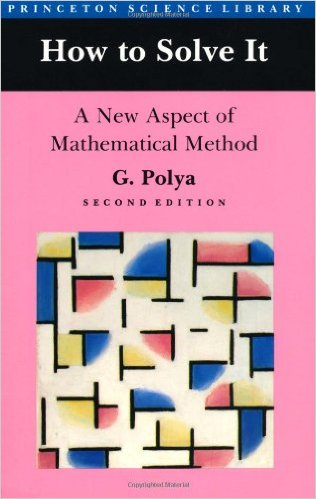
\includegraphics[width=1.6cm]{polya.jpg}
\end{center}

%\vspace{0.4cm}

\item<2-> We illustrate its problem-solving method with mathematical problems, but those
ideas can be applied to computer science and other domains as well.\\

%\vspace{0.4cm}

\item<3-> \emph{Microsoft} used to give Polya's book to all of its new programmers.

\end{itemize}

\end{frame}

\begin{frame}%[containsverbatim]
\frametitle{Three Examples}

We illustrate the method with several problems, the following three are recurring in this section:

\begin{enumerate}

\item<1-> How many zeroes are at the end of $1000!$.

\vspace{0.2cm}

\item<2-> Suppose that $X$ and $Y$ are two finite sets. Find a formula that relates
$|X|$, $|Y|$, $|X\cup Y|$ and $|X\cap Y|$.

\vspace{0.2cm}

\item<3-> Show that the equation $x^2 + y^2 = z^n$ has positive integer solutions for every $n = 1, 2, 3, \ldots$.

\end{enumerate}

\end{frame}

\subsection{Four Steps Plan}

\begin{frame}%[containsverbatim]
\frametitle{Polya's Four Steps Plan}

For solving any type
of problem, Polya gives a four-point plan:
\vspace{0.2cm}
\begin{enumerate}

\item<1-> Understand the problem.
\vspace{0.35cm}

\item<2-> Devise a plan.
\vspace{0.35cm}

\item<3-> Execute the plan.
\vspace{0.35cm}

\item<4-> Look back.

\end{enumerate}

\end{frame}

\subsection{Understand the Problem}

\begin{frame}%[containsverbatim]
\frametitle{Understand All the Words and Symbols in the Problem}

%The sooner you start coding your program the longer it is going to take.

%\scriptsize

%\vspace{0.5cm}

You have to cleary understand the problem description:\\
\vspace{0.1cm}
\begin{itemize}
\item<1-> The key to a solution may be to use the properties
of some particular definition.\\
\vspace{0.2cm}
%If you don't know that the definition provides that property,
%then you are unlikely to solve the problem.
\item<2-> So ensure you know and understand all the necessary \textbf{definitions and constraints} of the problem description.\\
\end{itemize}
%\vspace{0.5cm}

%\end{overprint}

%\textcolor{white}{Nothing in the problem description constrains you to stay within the bounds of the square. When you realize this, the problem is easy to solve.}
%\end{mdframed}
\end{frame}

\begin{frame}%[fragile]
\frametitle{Understand All the Words and Symbols in the Problem}

\begin{mdframed}[style=exampledefault]
Problem: You have to connect all nine points below with an unbroken path of four straight lines.
\end{mdframed}

\begin{overlayarea}{1\textwidth}{0.7\textheight}
\begin{center}
\includegraphics<1>[width=7cm]{nine_points.pdf}
\ifanswers
\includegraphics<2>[width=7cm]{nine_points_solution.pdf}
\fi
\end{center}
\end{overlayarea}


\end{frame}

\begin{frame}%[containsverbatim]
\frametitle{Draw a Picture}

\setbeamercovered{transparent=0}

The human mind is very good at working with images.
Pictures are excellent for
\begin{itemize}
\item<2-> Understanding the problem.

\item<2-> Developing intuition about a problem and subsequently suggesting a solution to it.
% In fact, a diagram
%is often essential in problems from geometry or physics.\\

\end{itemize}

\vspace{0.4cm}
\onslide<3->
For the second problem drawing a Venn diagram is very illuminating.
\vspace{-0.3cm}
\begin{overlayarea}{1\textwidth}{0.4\textheight}
\begin{center}
\includegraphics<3->[width=4.5cm]{venn_diagram.pdf}
\end{center}
\end{overlayarea}

\end{frame}

\begin{frame}%[containsverbatim]
\frametitle{Draw a Picture: Handshake Problem}

Mr. and Mrs Smith recently attended a party at which there were three other couples.
Various handshakes took place:
\begin{itemize}
\item<2-> No one shook hands with his/her own spouse.
\vspace{0.2cm}
\item<3-> No one shook hands with the same person twice.
\vspace{0.2cm}
\item<4-> No one shook his/her own hand.
\vspace{0.2cm}
\end{itemize}
\onslide<5->
After all the handshaking was finished, Mr. Smith asked each person, including his wife, how many hands he or she had shaken.
\onslide<6-> To his surprise, each gave a different answer.

\onslide<7->
\begin{mdframed}[style=exampledefault]
Problem: How many hands did Mrs. Smith shake?
\end{mdframed}

\end{frame}

\ifanswers
\begin{frame}%[containsverbatim]
\frametitle{Handshake Problem Solution}

First of all, the answers to Mr Smith's query must have been the numbers $0$, $1$, $2$, $3$, $4$, $5$ and $6$.

\begin{overlayarea}{1\textwidth}{0.7\textheight}
\begin{center}
\includegraphics<2>[width=7cm]{handshake.pdf}%
\includegraphics<3>[width=7cm]{handshake1.pdf}%
\includegraphics<4>[width=7cm]{handshake2.pdf}%
\includegraphics<5>[width=7cm]{handshake3.pdf}%
\includegraphics<6>[width=7cm]{handshake4.pdf}%
\includegraphics<7>[width=7cm]{handshake5.pdf}%
\includegraphics<8>[width=7cm]{handshake6.pdf}%
\includegraphics<9>[width=7cm]{handshake7.pdf}%
\includegraphics<10>[width=7cm]{handshake8.pdf}%
\includegraphics<11>[width=7cm]{handshake9.pdf}%
\includegraphics<12>[width=7cm]{handshake10.pdf}%
\includegraphics<13>[width=7cm]{handshake11.pdf}%
\end{center}
\end{overlayarea}

\end{frame}

\fi

\subsection{Devising a Plan}

\begin{frame}%[containsverbatim]
\frametitle{Devising a Plan}

\begin{itemize}

\item Once the problem is understood construct a plan to solve it.

\begin{center}
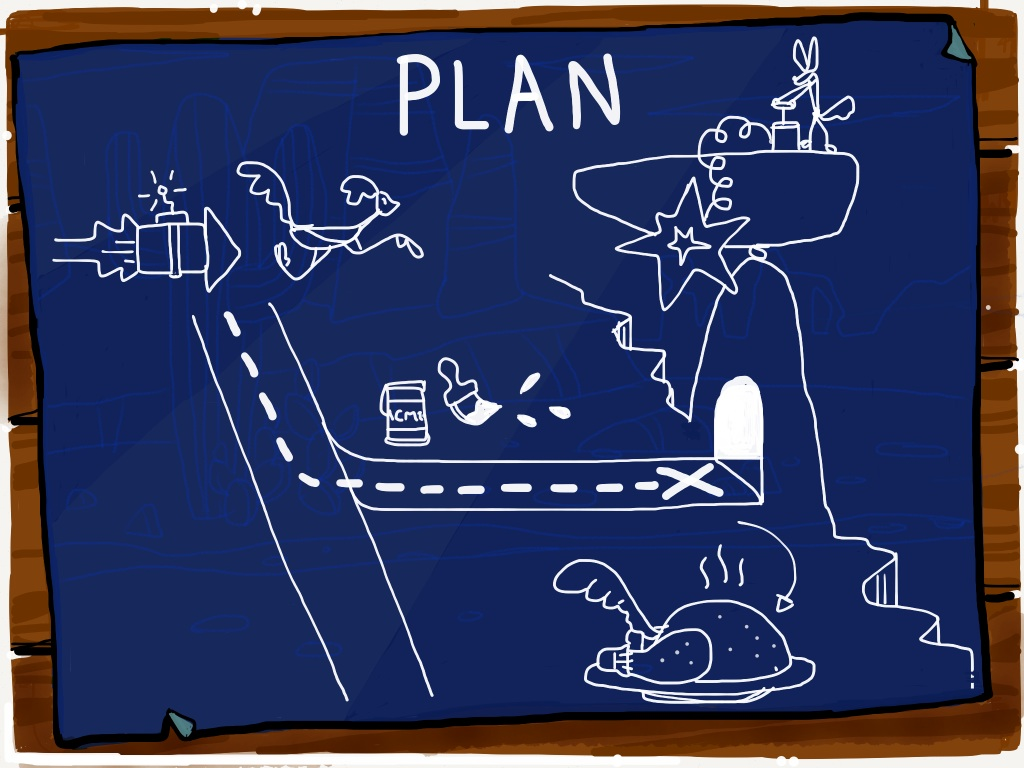
\includegraphics[width=6cm]{bipbip.jpg}
\end{center}

\vspace{0.5cm}

\item<2-> Polya gives some general ideas to devise a plan to tackle the problem (in the following slides).

\end{itemize}

\end{frame}

\begin{frame}%[containsverbatim]
\frametitle{Work with Initial and Special Cases}

\begin{itemize}
\item Many problems will have some form of \textbf{index}.\\
\begin{itemize}
\item<1-> In the third problem ($x^2 + y^2 = z^n$), we have to find integers $x$, $y$ and $z$ for every possible $n$: the index is $n$.
\end{itemize}

\vspace{0.5cm}

\item<2-> In these indexed problems you should try to solve the problem in the initial cases, e.g.
$n = 1$, $2$ and $3$.
\begin{itemize}
\item<2-> This will not necessarily give you the general answer but allows insight
and a ``feel'' for the problem.
\end{itemize}
\end{itemize}

%% \begin{itemize}
%% \item If $n = 1$ we have to find solutions to $x^2 + y^2 = z$. This is easy in this case.\\
%% \vspace{0.2cm}
%% \item For $n = 2$ we have to solve $x^2 + y^2 = z^2$. This is the famous Pythagoras equation, for
%% which we have many solutions.\\
%% \vspace{0.2cm}
%% \item For $n = 3$ we have to solve $x^2 + y^2 = z^3$. Because it seems to be less obvious, we can
%% try to use the $n = 2$ case to provide a solution.
%% \end{itemize}

\end{frame}

\begin{frame}%[containsverbatim]
\frametitle{Work with Initial and Special Cases}

\begin{center}
\includegraphics<1>[width=9cm]{polya_initial_special_cases.pdf}%
\includegraphics<2>[width=9cm]{polya_initial_special_cases1.pdf}%
\includegraphics<3>[width=9cm]{polya_initial_special_cases2.pdf}%
\end{center}

%% \begin{itemize}
%% \item If $n = 1$ we have to find solutions to $x^2 + y^2 = z$. This is easy in this case.\\
%% \vspace{0.2cm}
%% \item For $n = 2$ we have to solve $x^2 + y^2 = z^2$. This is the famous Pythagoras equation, for
%% which we have many solutions.\\
%% \vspace{0.2cm}
%% \item For $n = 3$ we have to solve $x^2 + y^2 = z^3$. Because it seems to be less obvious, we can
%% try to use the $n = 2$ case to provide a solution.
%% \end{itemize}

\end{frame}

\begin{frame}%[containsverbatim]
\frametitle{Work with a Concrete Case}


\begin{itemize}
\item Look at a concrete case.
%In a similar way to the idea on the previous slide, for an abstract problem look at a concrete case.\\
%\vspace{0.2cm}

\begin{itemize}
%In a problem concerned with sets take a specific set. So for the second problem take a set where
\item<1-> For the second problem, let's $X = \{a, b, c, d\}$ and $Y = \{b, d, e, f, g\}$. We have% In this case we see that

\begin{itemize}
\item<2-> $|X| = 4$, $|Y| = 5$.

\item<2-> $|X \cup Y| = |\{a, b, c, d, e, f, g\}| = 7$ and $|X \cap Y| = |\{b, d\}| = 2$.

\end{itemize}

\item<3-> So we need a formula that relates $4$, $5$, $2$ and $7$.

\item<3-> Play around with some other examples if you don't see a pattern.

\end{itemize}

%% So we need
%% a formula that relates $4$, $5$, $2$ and $7$. Play around with some other examples if you don't
%% see a pattern. Vary $X$ and $Y$ by an element or two and see how the cardinalities change.\\

\vspace{0.5cm}

\item<4-> The examination of specific cases is intended to provide insight and frequently unlocks the problem.

\end{itemize}

\end{frame}

\begin{frame}%[containsverbatim]
\frametitle{Example: Matches Game from Fort Boyard}

You have $\textbf{n}$ matches in front of you and you can take between $\textbf{1}$ and $\textbf{k}$ matches when it is your turn to play. The player
who cannot move loses.
\begin{mdframed}[style=exampledefault]
Problem: How to play optimaly?
\end{mdframed}

\begin{overlayarea}{1\textwidth}{0.5\textheight}
\begin{center}
\includegraphics<2>[width=8cm]{matches.pdf}%
\end{center}
\end{overlayarea}

\end{frame}

\begin{frame}%[containsverbatim]
\frametitle{Example: Matches game from Fort Boyard}

\begin{itemize}

\item To work with a concrete case, let's fix $k$ to $1$.

\vspace{0.5cm}

\item<2-> Now that we have a concrete game, let's try with more and more matches.

\end{itemize}

\end{frame}

\begin{frame}%[containsverbatim]
\frametitle{Example: Matches game from Fort Boyard}
\only<1>{
\begin{center}
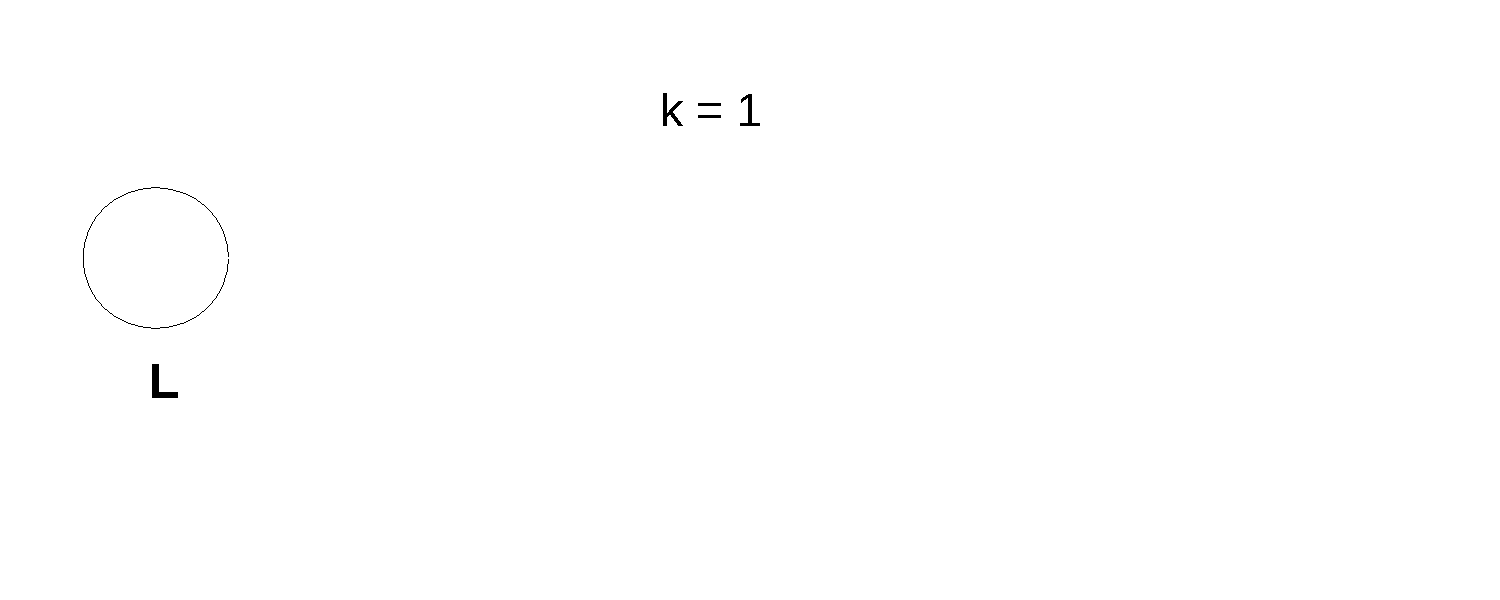
\includegraphics[width=11cm]{matches1.pdf}%
\end{center}
}
\only<2>{
\begin{center}
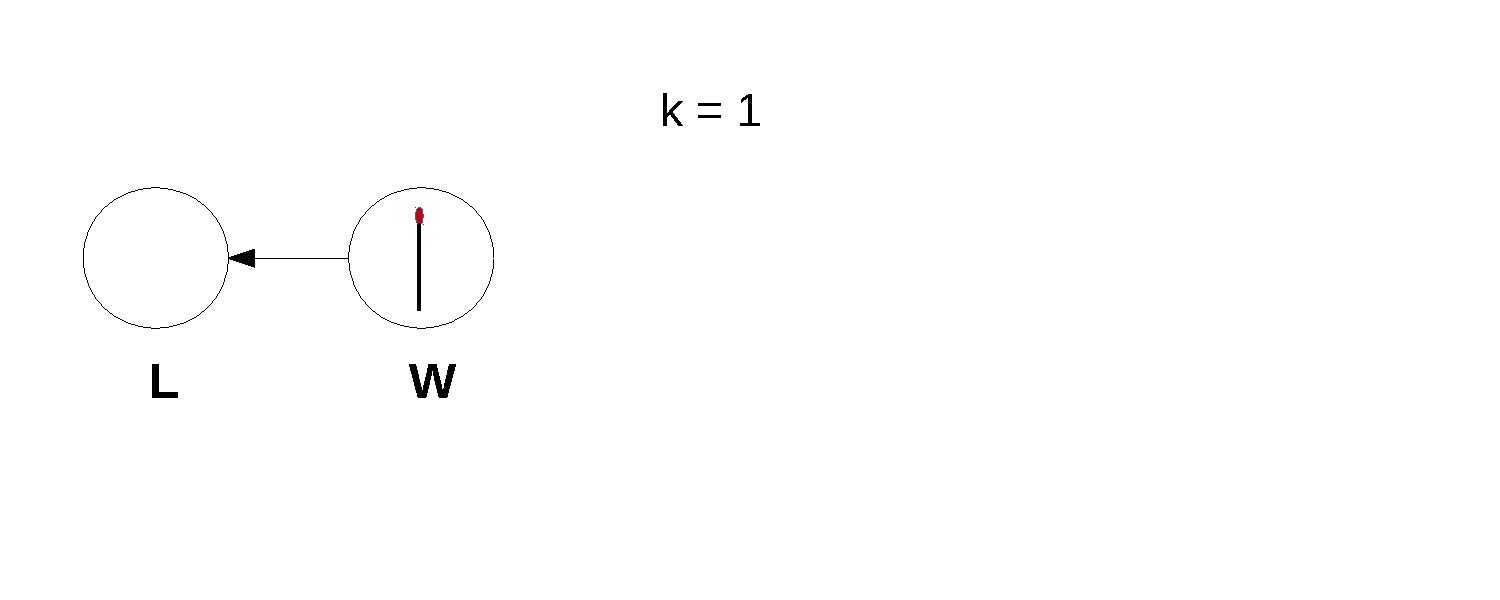
\includegraphics[width=11cm]{matches2.pdf}%
\end{center}
}
\only<3>{
\begin{center}
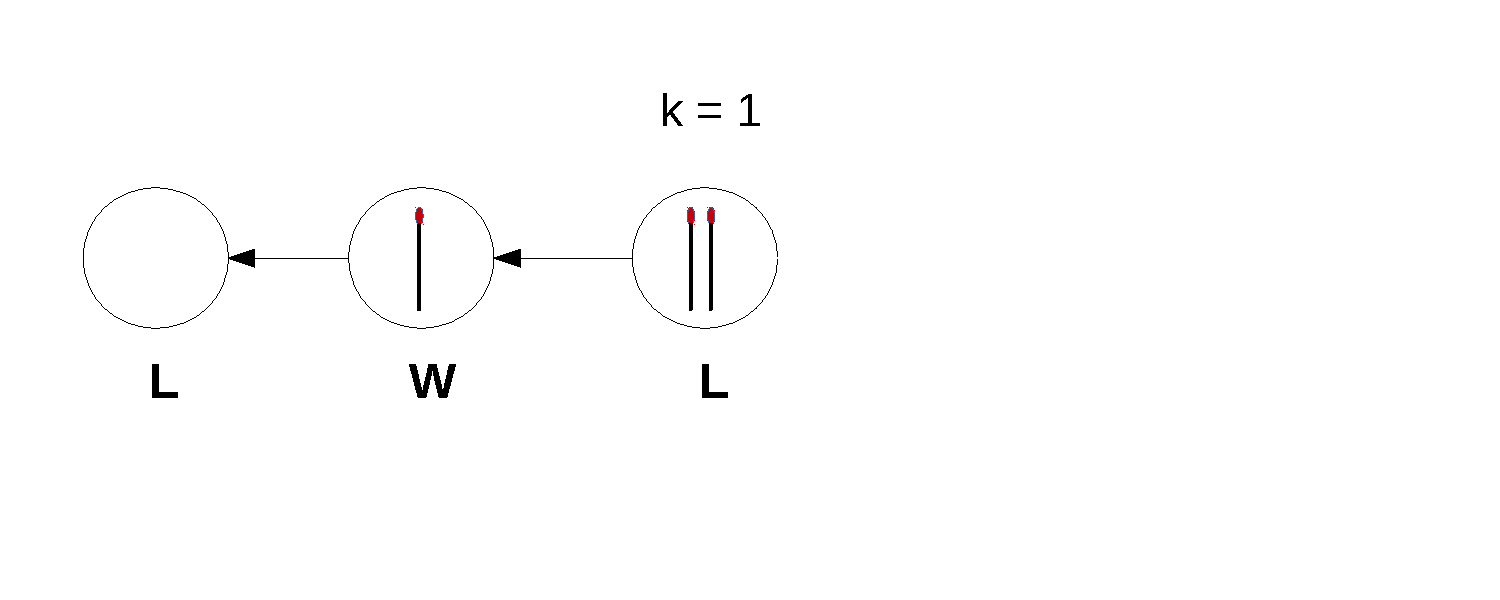
\includegraphics[width=11cm]{matches3.pdf}%
\end{center}
}
\only<4>{
\begin{center}
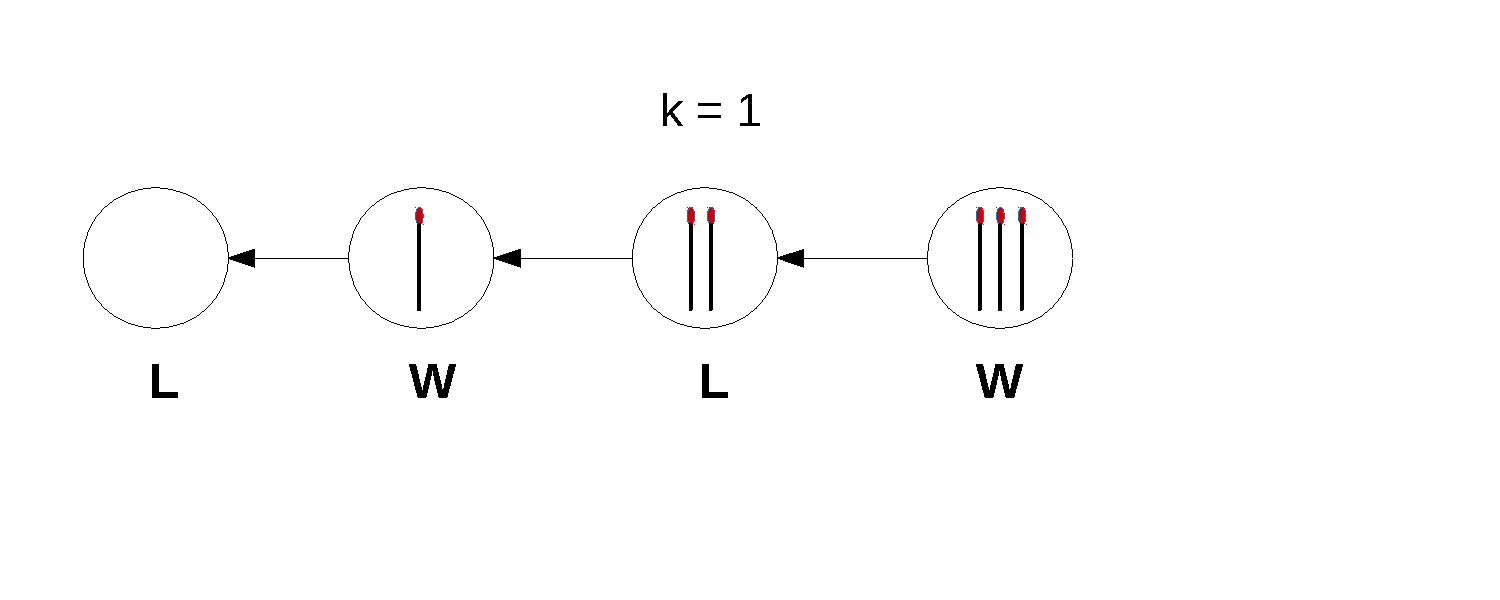
\includegraphics[width=11cm]{matches4.pdf}%
\end{center}
}
\only<5>{
\begin{center}
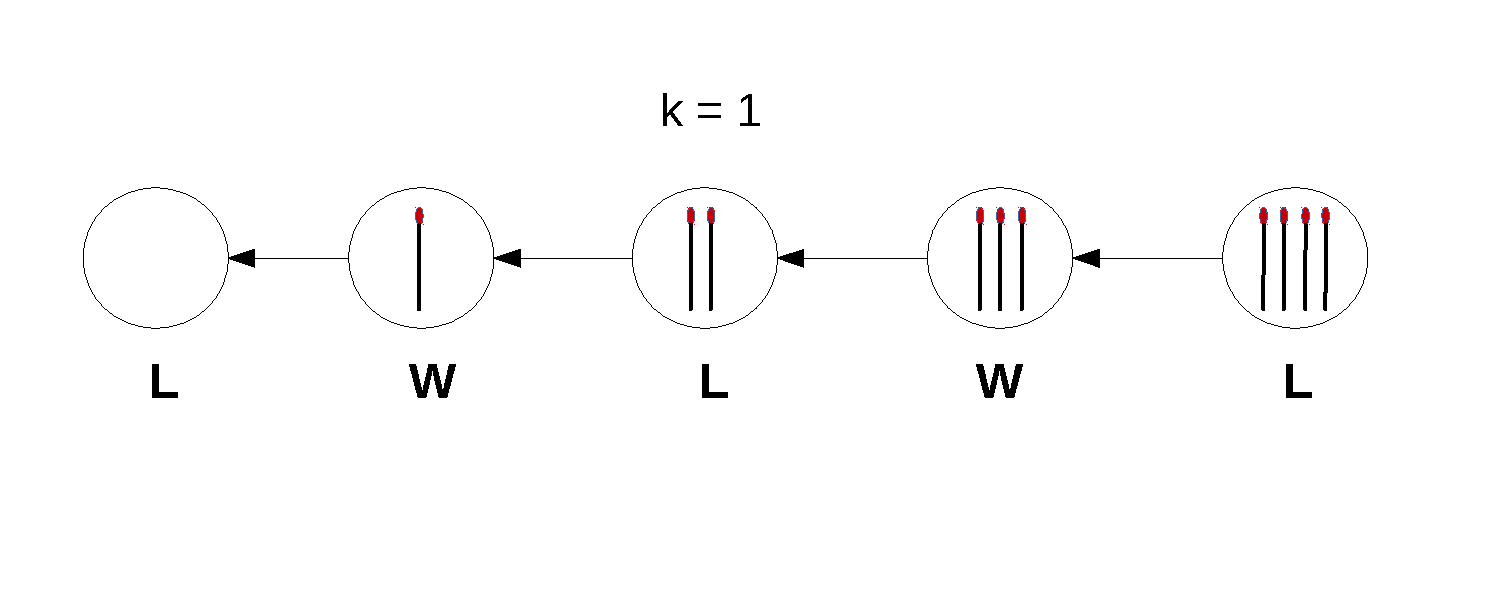
\includegraphics[width=11cm]{matches5.pdf}%
\end{center}
}

\end{frame}

\begin{frame}%[containsverbatim]
\frametitle{Example: Matches game from Fort Boyard}

\begin{center}
\includegraphics<1>[width=11cm]{matches21.pdf}%
\includegraphics<2>[width=11cm]{matches22.pdf}%
\includegraphics<3>[width=11cm]{matches23.pdf}%
\includegraphics<4>[width=11cm]{matches24.pdf}%
\includegraphics<5>[width=11cm]{matches25.pdf}%
\end{center}

\end{frame}

\begin{frame}%[containsverbatim]
\frametitle{\exo}

\vspace{1cm}
\begin{mdframed}[style=exampledefault]
Problem: How many ways can a $1 \times n$ rectangle be filled by nonoverlapping $1 \times 1$ and $1 \times 2$ rectangles?
\end{mdframed}
\vspace{1cm}

\begin{center}
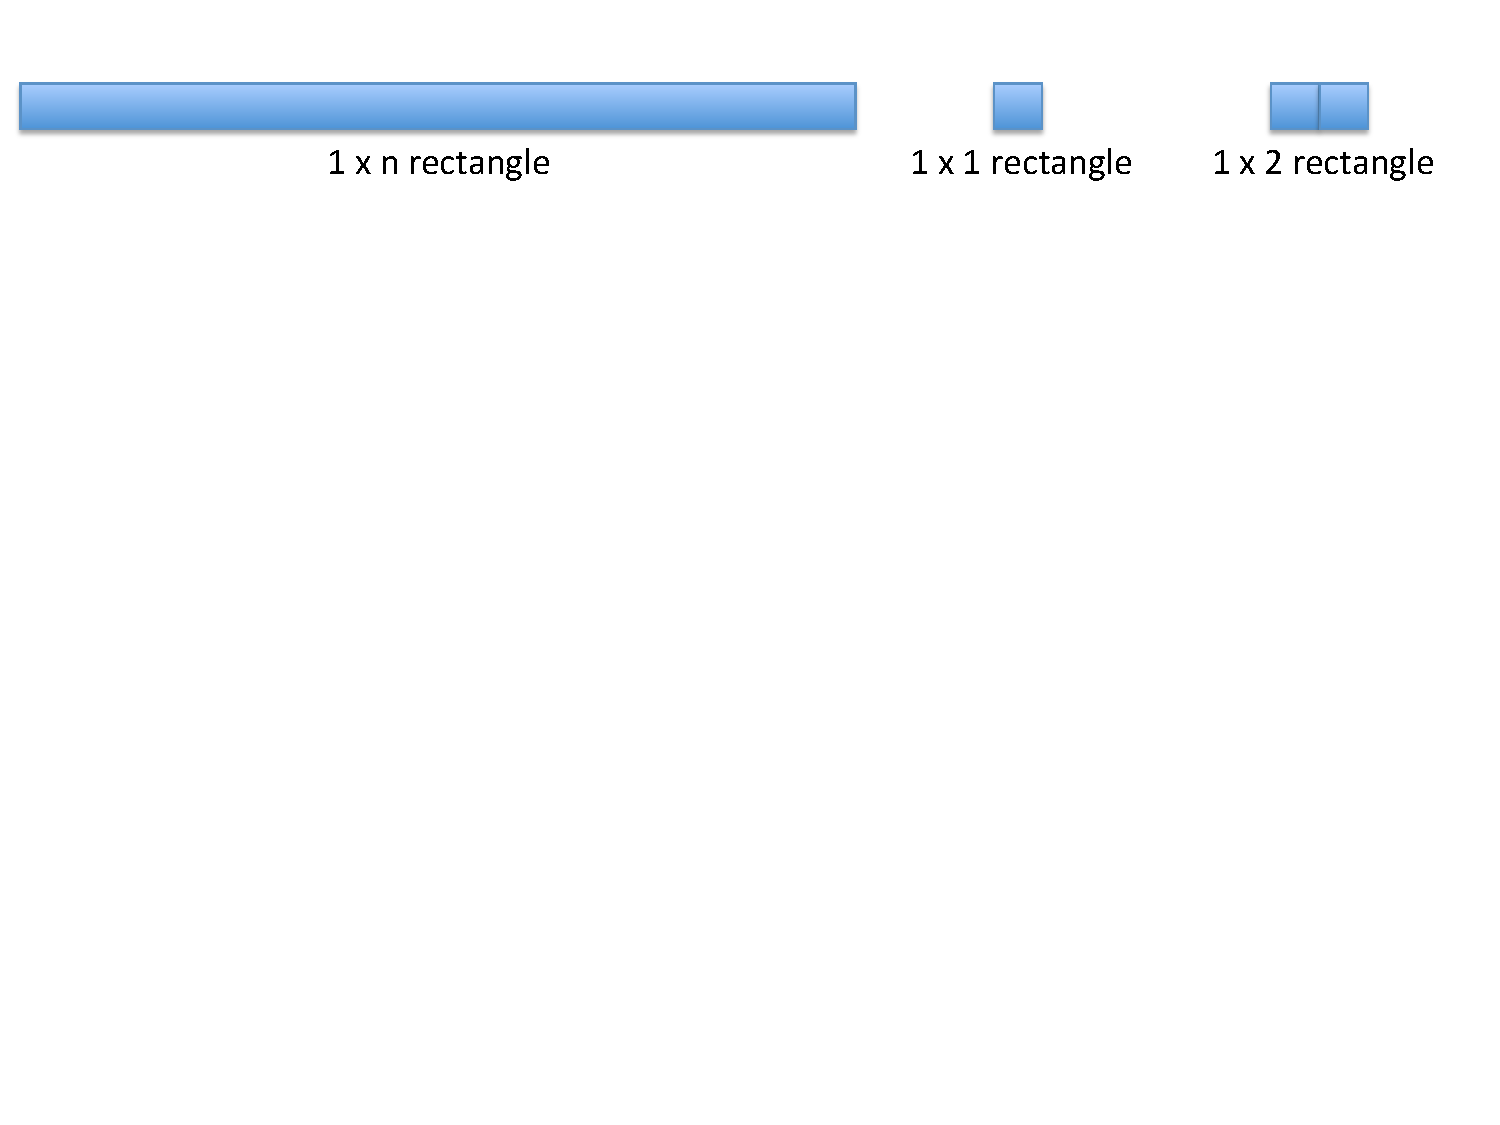
\includegraphics[width=12cm]{rectangle.pdf}%
\end{center}

\end{frame}

\ifanswers

\begin{frame}%[containsverbatim]
\frametitle{Solution}

%\vspace{1cm}
How many ways can a $1 \times n$ rectangle be filled by nonoverlapping $1 \times 1$ and $1 \times 2$ rectangles?

\begin{center}
\includegraphics<1>[width=8cm]{fibo_tilling.pdf}%
\includegraphics<2>[width=8cm]{fibo_tilling1.pdf}%
\includegraphics<3>[width=8cm]{fibo_tilling2.pdf}%
\includegraphics<4>[width=8cm]{fibo_tilling3.pdf}%
\includegraphics<5>[width=8cm]{fibo_tilling4.pdf}%
\end{center}

%% \begin{itemize}

%% \item \textbf{$n = 1$:}

%% \end{itemize}

\end{frame}

\begin{frame}%[containsverbatim]
\frametitle{Solution}

%\vspace{1cm}

When you fill an $1\times n$, with $n\ge 2$, rectangle
\begin{tabular}{|c:c:c:c:c}
\hline
& & & & $\cdots$ \\
\hline
\end{tabular}
, you only have two choices for the beginning of the rectangle:\\

\vspace{0.3cm}

\begin{itemize}

\item<2-> You put an $1\times 1$ rectangle \begin{tabular}{|c|c:c:c:c}
\hline
& & & & $\cdots$ \\
\hline
\end{tabular} and it remains to fill an $1\times (n-1)$ rectangle.\\

\vspace{0.5cm}

\item<3-> You put an $1\times2$ rectangle \begin{tabular}{|cc|c:c:c}
\hline
& & & & $\cdots$ \\
\hline
\end{tabular} and it remains to fill an $1\times (n-2)$ rectangle.\\

\end{itemize}
\onslide<3->
\vspace{0.5cm}

Therefore, if $n\ge 2$, we have $s_n = s_{n-1} + s_{n-2}$. You can check that $s_1 = 1$ and $s_0 = 1$.

\end{frame}

\fi

\begin{frame}%[containsverbatim]
\frametitle{Solve an Easier Problem}

%This is similar to working with a special case.
With the experience from solving an easier problem it might be possible to solve the general one.\\

%\vspace{0.4cm}

\begin{overlayarea}{1\textwidth}{0.7\textheight}
\begin{center}
\includegraphics<2>[width=8cm]{polya_easier.pdf}%
\includegraphics<3>[width=8cm]{polya_easier1.pdf}%
\end{center}
\end{overlayarea}

%% So for example, in the first problem it may be easier to work with $10!$ rather than $1000!$. Try it
%% and see what happens. It may suggest some ideas. In the third problem consider what happens
%% if $z$ is odd or even.

\end{frame}


\begin{frame}%[containsverbatim]
\frametitle{Work Backwards and Forwards}

\begin{center}
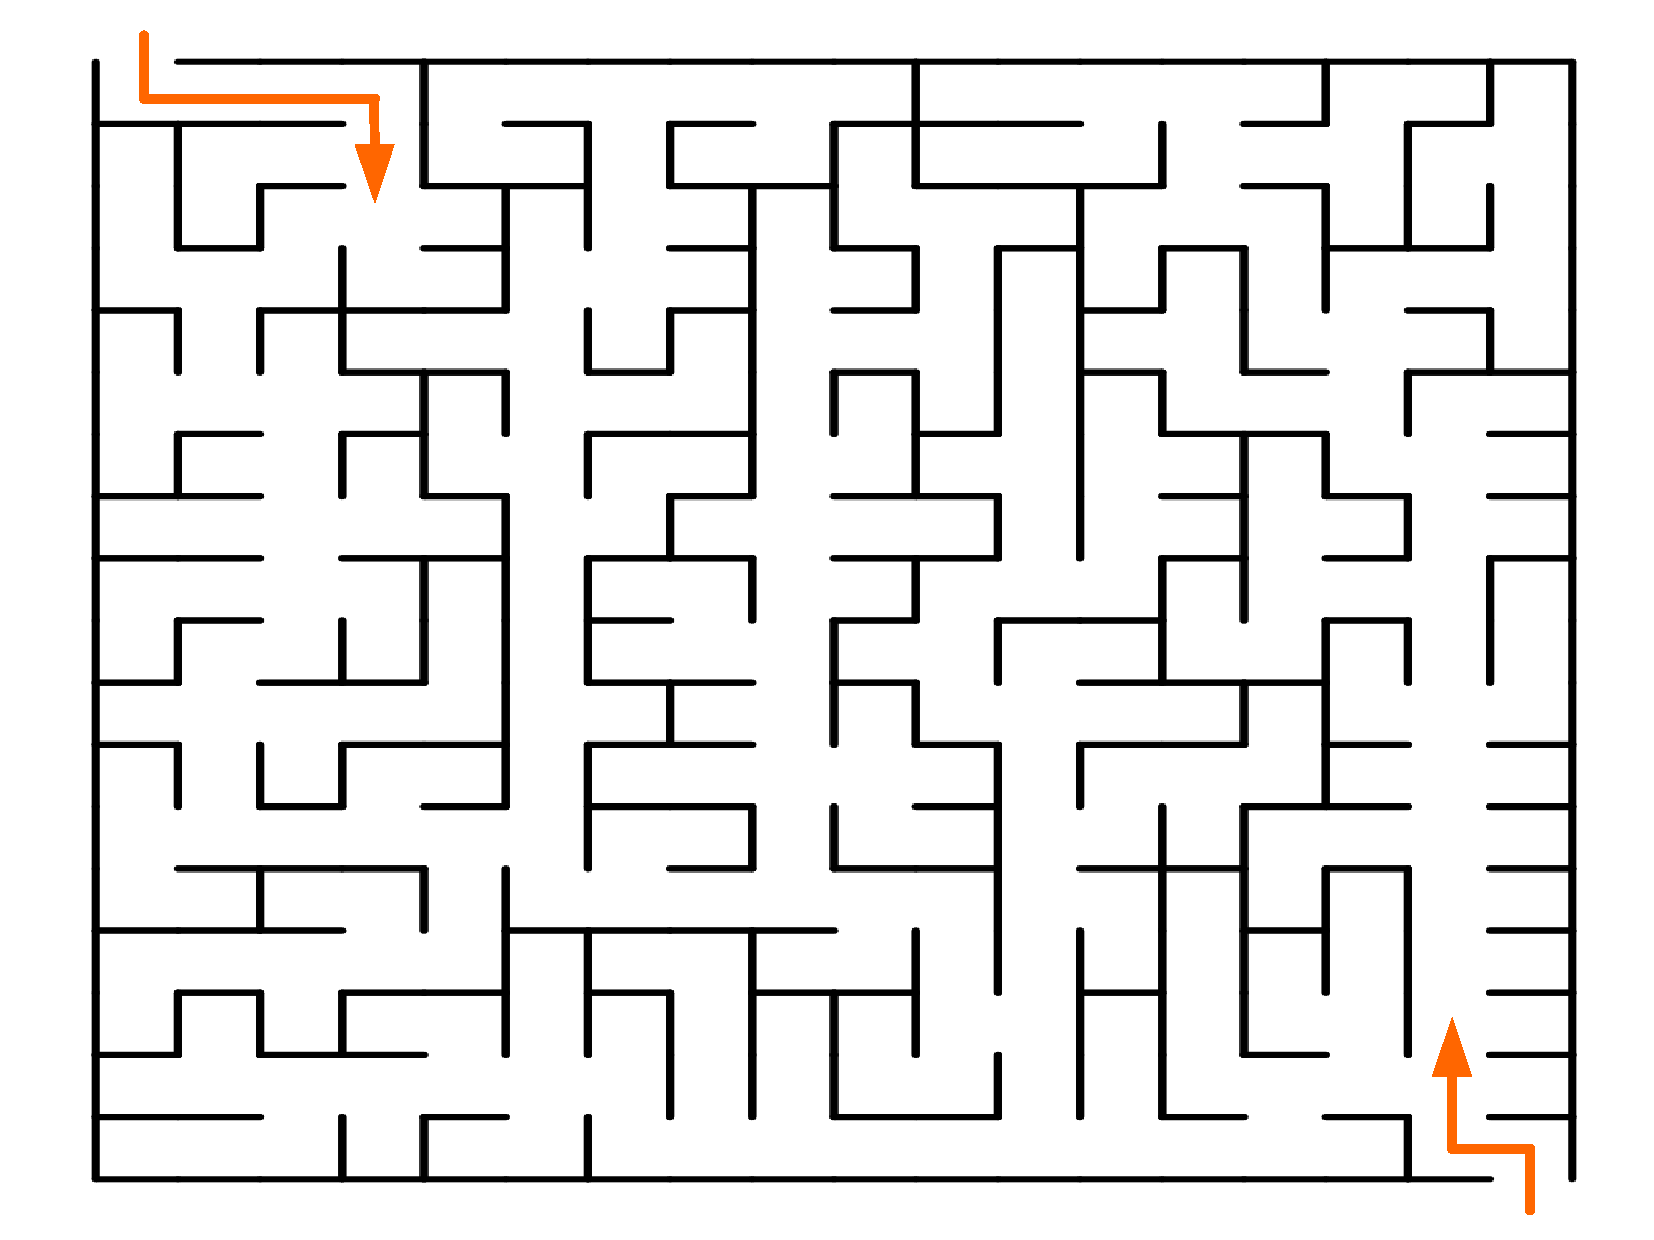
\includegraphics[width=4.5cm]{maze.pdf}%
\end{center}

\begin{itemize}

\item You can start with the conclusion and try to think what this would imply.

\vspace{0.15cm}

\item<2-> Once the solution becomes clearer rewrite with the assumptions going to the conclusion.

\end{itemize}


%% In finding the solution, you do not have to begin with the assumptions and work towards
%% the conclusion.You can start with the conclusion and try to think what this would imply.\\

%% \vspace{0.5cm}

%% In this way one can work towards the assumptions. Once the solution becomes clear rewrite
%% with the assumptions going to the conclusion.

\end{frame}

\begin{frame}%[containsverbatim]
\frametitle{Work Backwards and Forwards}

%% For example, if $1000!$ has exactly $n$ zeroes at the end what does that imply?\\
%% \vspace{0.3cm}
%% It means that $1000! = y \times 10^n$ for some $y$ where $y$ does
%% not end in a zero. Thus, from $1000!$ we need to take out factors of $10$.\\
%% \vspace{0.3cm}
%% Now we look at
%% $1000!$ and see from the definition how factors of $10$ might arise.\\
%% \vspace{0.3cm}

\begin{center}
\includegraphics<1>[width=7.5cm]{polya_backward_forward.pdf}%
\includegraphics<2->[width=7.5cm]{polya_backward_forward1.pdf}%
\end{center}

\onslide<3->
Proceeding in this way,
i.e. backwards and forwards, we can produce an argument that \textbf{``meets in the middle''}.

\end{frame}

\begin{frame}%[containsverbatim]
\frametitle{Working Backwards Example}

 In a round-robin tournament with $n$ players $P_1$, $P_2$, \ldots, $P_n$, where $n > 1$,
\begin{itemize}
\item<2-> Each player plays one game with each of the other players.
\item<3-> Rules are such that no ties can occur.
\item<4-> Let $W_r$ be the number of games won by player $P_r$.
\item<5-> Let $L_r$ be the number of games lost by player $P_r$.
\end{itemize}
\onslide<6->
\begin{mdframed}[style=exampledefault]
Problem: Show that
$$
\sum_{r = 1}^{n} W_r^2 = \sum_{r = 1}^{n} L_r^2.
$$
\end{mdframed}

\end{frame}

\begin{frame}%[containsverbatim]
\frametitle{Working Backwards Example}

\scriptsize

Suppose $\sum_{r = 1}^{n} W_r^2 = \sum_{r = 1}^{n} L_r^2$. Then,

\onslide<2->

$$
\sum_{r = 1}^{n} (W_r^2 - L_r^2) = 0,
$$

\onslide<3->

$$
\sum_{r = 1}^{n} (W_r - L_r)(W_r + L_r) = 0,
$$

\onslide<4->

But $W_r + L_r = n - 1$ for each $r$, so

\onslide<5->
$$
(n - 1)\sum_{r = 1}^{n} (W_r - L_r) = 0,
$$

\onslide<6->
$$
\sum_{r = 1}^{n} (W_r - L_r) = 0,
$$

\onslide<7->
$$
\sum_{r = 1}^{n} W_r = \sum_{r = 1}^{n} L_r
$$

which is true. We can now reverse this argument.

\end{frame}

\begin{frame}%[containsverbatim]
\frametitle{\exo}

\uvalink{10360}{https://uva.onlinejudge.org/index.php?option=com_onlinejudge&Itemid=8&category=15&page=show_problem&problem=1301}

\end{frame}

\ifanswers

\begin{frame}
\frametitle{10360 Solution}

\footnotesize

If we try to solve the problem in the forward direction,
due to the problem constraints, it can take up to $1025^2 \times 50^2 = 2,626,562,500$ iterations for one
test case!

\begin{overlayarea}{1\textwidth}{0.6\textheight}
\begin{center}
\includegraphics<1>[width=6cm]{rat_attacks.pdf}%
\includegraphics<2>[width=6cm]{rat_attacks1.pdf}%
\includegraphics<3>[width=6cm]{rat_attacks2.pdf}%
\includegraphics<4>[width=6cm]{rat_attacks3.pdf}%
\includegraphics<5>[width=6cm]{rat_attacks4.pdf}%
\includegraphics<6>[width=6cm]{rat_attacks5.pdf}%
\includegraphics<7>[width=6cm]{rat_attacks6.pdf}%
\end{center}
\end{overlayarea}


\end{frame}

\begin{frame}
\frametitle{10360 Solution}

\begin{itemize}
\item If we solve the problem in the backward direction, for each rat, we increment the location
where a bomb would kill this rat.

\vspace{0.2cm}

\item<2-> We can now scan each location and pick the one with the maximum value to place the bomb.

\vspace{0.2cm}

\item<3-> The maximum number of iterations we can get is $20000 \times 50^2 + 1025^2 = 51,050,625$. It is
more than $50$ times faster!

\end{itemize}

\end{frame}

\begin{frame}%[fragile]
\frametitle{10360 Solution}

\begin{center}
\includegraphics<1>[width=8cm]{rat_attacks7.pdf}%
\includegraphics<2>[width=8cm]{rat_attacks8.pdf}%
\includegraphics<3>[width=8cm]{rat_attacks9.pdf}%
\includegraphics<4>[width=8cm]{rat_attacks10.pdf}%
\includegraphics<5>[width=8cm]{rat_attacks11.pdf}%
\includegraphics<6>[width=8cm]{rat_attacks12.pdf}%
\includegraphics<7>[width=8cm]{rat_attacks13.pdf}%
\includegraphics<8>[width=8cm]{rat_attacks14.pdf}%
\includegraphics<9>[width=8cm]{rat_attacks15.pdf}%
\includegraphics<10>[width=8cm]{rat_attacks16.pdf}%
\includegraphics<11>[width=8cm]{rat_attacks17.pdf}%
\includegraphics<12>[width=8cm]{rat_attacks18.pdf}%
\includegraphics<13>[width=8cm]{rat_attacks19.pdf}%
\includegraphics<14>[width=8cm]{rat_attacks20.pdf}%
\includegraphics<15>[width=8cm]{rat_attacks21.pdf}%
\includegraphics<16>[width=8cm]{rat_attacks22.pdf}%
\includegraphics<17>[width=8cm]{rat_attacks23.pdf}%
\end{center}

\end{frame}


\begin{frame}[containsverbatim]
\frametitle{10360 Solution Implementation}
\scriptsize

\begin{lstlisting}
int main(int argc, char *argv[]) {
  int tc; cin >> tc;
  while (tc--)
  {
    int d, N;
    cin >> d >> N;
    int nb_rats_killed[1025][1025]{};
    for (int i = 0; i < N; ++i)
    {
      int x, y, nb_rats;
      cin >> x >> y >> nb_rats;
      for (int bx = max(0, x - d); bx <= min(1024, x + d); ++bx)
      {
        for (int by = max(0, y - d); by <= min(1024, y + d); ++by)
        {
          nb_rats_killed[bx][by] += nb_rats;
        }
      }
    }
    // ...
\end{lstlisting}

\end{frame}

\begin{frame}[containsverbatim]
\frametitle{10360 Solution Implementation}
\scriptsize

\begin{lstlisting}
    // ...
    int best_x = 0, best_y = 0;
    for (int x = 0; x < 1025; ++x)
    {
      for (int y = 0; y < 1025; ++y)
      {
        if (nb_rats_killed[x][y] > nb_rats_killed[best_x][best_y])
        {
          best_x = x;
          best_y = y;
        }
      }
    }
    cout << best_x << " " << best_y << " "
         << nb_rats_killed[best_x][best_y] << endl;
  }
  return 0;
}
\end{lstlisting}

\end{frame}

\fi

\begin{frame}%[containsverbatim]
\frametitle{Meet in the Middle Example}

\setbeamercovered{transparent=0}

\begin{mdframed}[style=exampledefault]
Problem: Given a set $\mathcal{S}$ of $n$ ($1 \le n \le 40$) integers each of them at most $10^{12}$, and given an integer $0 \le I \le 10^{18}$, determine
the largest subset sum of $\mathcal{S}$ less than or equal to $I$.
\end{mdframed}

\begin{overlayarea}{1\textwidth}{0.6\textheight}
%\begin{center}
\onslide<2->
\huge
$$
I = 91
$$
\Large
\only<2>{
$$
\mathcal{S} = \{ -8, 12, 1, 2, 3, -25, 32, 18, 30, -40 \}
$$
}
\only<3>{
$$
\mathcal{S} = \{ \textcolor{red}{-8}, \textcolor{red}{12}, \textcolor{red}{1}, \textcolor{red}{2}, \textcolor{red}{3}, -25, \textcolor{red}{32}, \textcolor{red}{18}, \textcolor{red}{30}, -40 \}
$$
$$
\textrm{best sum} = 90
$$
}
%\end{center}
\end{overlayarea}

\end{frame}

\begin{frame}%[containsverbatim]
\frametitle{Meet in the Middle Example}

\begin{itemize}

\item It is way too slow to brute-force the $2^{40}$ subset sums to get the right answer.

\vspace{0.2cm}

\item<2-> We can split $\mathcal{S}$ into two sets $A$ and $B$ with $|A| = \lfloor \frac{|\mathcal{S}|}{2} \rfloor$
and $|B| = \lceil \frac{|\mathcal{S}|}{2} \rceil$.

\vspace{0.2cm}

\item<3-> We can compute all subset sums for $A$ and $B$ and store the results in two arrays \texttt{X} and \texttt{Y}.

\vspace{0.2cm}

\item<4-> We can now iterate over the elements \texttt{x} of \texttt{X} and use binary search to find the largest element \texttt{y} of \texttt{Y} such that
$\texttt{x} + \texttt{y} \le I$.

\vspace{0.2cm}

\item<5-> The complexity is $O(2^{\frac{n}{2}} \times n)$.

\end{itemize}

\end{frame}

\begin{frame}[containsverbatim]
\frametitle{Meet in the Middle Example Implementation}

\scriptsize

\begin{lstlisting}
int main(int argc, char *argv[]) {
  int N;
  long long I;
  cin >> N >> I;
  vector<long long> S(N);
  long long best_sum = 0;
  for (int i = 0; i < N; ++i)
  {
    cin >> S[i];
  }
  vector<long long> X = all_subset_sums({S.begin(), S.begin() + N / 2});
  vector<long long> Y = all_subset_sums({S.begin() + N / 2, S.end()});
  for (long long v : X)
  {
    long long sum = v + binary_search(Y, I - v);
    if (sum > best_sum && sum <= I) best_sum = sum;
  }
  cout << best_sum << endl;
  return 0;
}
\end{lstlisting}

\end{frame}

\begin{frame}[containsverbatim]
\frametitle{Meet in the Middle Example Implementation}

\scriptsize

\begin{lstlisting}
vector<long long> all_subset_sums(const vector<long long>& numbers)
{
  set<long long> res;
  for (int subset = 0; subset < (1 << numbers.size()); ++subset)
  {
    long long sum = 0;
    for (unsigned int j = 0; j < numbers.size(); ++j)
    {
      if (subset & (1 << j)) sum += numbers[j];
    }
    res.insert(sum);
  }
  return {res.begin(), res.end()};
}
\end{lstlisting}

\end{frame}

\begin{frame}[containsverbatim]
\frametitle{Meet in the Middle Example Implementation}

\scriptsize

\begin{lstlisting}
long long binary_search(const vector<long long>& array, long long val)
{
  int start = 0;
  int end   = array.size() - 1;
  if (array[end] <= val) return array[end];
  if (array[start] >= val) return array[start];
  while (start <= end)
  {
    int middle = start + (end - start) / 2;
    if (array[middle] == val) return val;
    if (array[middle] < val) start = middle + 1;
    else end = middle - 1;
  }
  return array[end];
}
\end{lstlisting}

\end{frame}

\begin{frame}%[containsverbatim]
\frametitle{\exo}

\codeforceslink{Lizard Era: Beginning}{http://www.codeforces.com/problemset/problem/585/D}

\end{frame}

\ifanswers

\begin{frame}[fragile]
\frametitle{Lizard Era: Beginning Solution}

\setbeamercovered{transparent=0}

\footnotesize

\begin{itemize}

\item Each task (line) contains three integers $l_i$, $m_i$ and $w_i$. We have to choose two integers amongst those three, so we have ${{3}\choose{2}} = 3$ choices.

\item<2-> If $n$ is small, we can brute-force the solution. For the first example,
\begin{verbatim}
     3
     1 0 0
     0 1 0
     0 0 1
\end{verbatim}
we would get
\vspace{-0.2cm}
\begin{overlayarea}{1\textwidth}{0.25\textheight}
\begin{center}
\includegraphics<3>[width=4cm]{lizard_era.pdf}%
\includegraphics<4>[width=4cm]{lizard_era1.pdf}%
\includegraphics<5>[width=4cm]{lizard_era2.pdf}%
\includegraphics<6>[width=4cm]{lizard_era3.pdf}%
\includegraphics<7>[width=4cm]{lizard_era4.pdf}%
\includegraphics<8>[width=4cm]{lizard_era5.pdf}%
\includegraphics<9>[width=4cm]{lizard_era6.pdf}%
\includegraphics<10>[width=4cm]{lizard_era7.pdf}%
\includegraphics<11>[width=4cm]{lizard_era8.pdf}%
\includegraphics<12->[width=4cm]{lizard_era9.pdf}%
\end{center}
\end{overlayarea}
\onslide<13->
And so on.

\item<13-> But if $n = 25$, we have $3^{25} = 847,288,609,443$ combinations to test!

\end{itemize}

\end{frame}

\begin{frame}[fragile]
\frametitle{Lizard Era: Beginning Solution}

\footnotesize

\begin{itemize}

\item We use the \textbf{meet in the middle} strategy and split the tasks into two sets.

\vspace{0.2cm}

\item<2-> Now the maximum number of combinations for a set is $3^{13} = 1,594,323$
and we can brute-force each of the two sets of tasks.

\vspace{0.2cm}

\item<3-> We need to combine the results from the two sets of tasks.
\begin{itemize}
\footnotesize
\item<3-> Let $(a_1,b_1,c_1)$ be the sum of attitudes
for Lynn, Melina and Worrigan for one of the assignements of the first set of tasks.

\vspace{0.1cm}

\item<3-> Let $(a_2,b_2,c_2)$ be the sum of attitudes
for Lynn, Melina and Worrigan for one of the assignements of the second set of tasks.

\vspace{0.1cm}

\item<4-> To combine these two results, we must have
$$
a_1 + a_2 = b_1 + b_2 = c_1 + c_2.
$$

\item<5-> This is equivalent to: $a_1 - b_1 = b_2 - a_2$ and $b_1 - c_1 = c_2 - b_2$.

\end{itemize}

\end{itemize}

\end{frame}

\begin{frame}
\frametitle{Lizard Era: Beginning Solution}

\begin{center}
\includegraphics<1>[width=10cm]{lizard_era12.pdf}%
\includegraphics<2>[width=10cm]{lizard_era13.pdf}%
\includegraphics<3>[width=10cm]{lizard_era14.pdf}%
\includegraphics<4>[width=10cm]{lizard_era15.pdf}%
\includegraphics<5>[width=10cm]{lizard_era16.pdf}%
\includegraphics<6>[width=10cm]{lizard_era17.pdf}%
\includegraphics<7>[width=10cm]{lizard_era18.pdf}%
\includegraphics<8>[width=10cm]{lizard_era19.pdf}%
\includegraphics<9>[width=10cm]{lizard_era20.pdf}%
\includegraphics<10>[width=10cm]{lizard_era21.pdf}%
\includegraphics<11>[width=10cm]{lizard_era22.pdf}%
\includegraphics<12>[width=10cm]{lizard_era23.pdf}%
\includegraphics<13>[width=10cm]{lizard_era24.pdf}%
\includegraphics<14>[width=10cm]{lizard_era25.pdf}%
\includegraphics<15>[width=10cm]{lizard_era26.pdf}%
\includegraphics<16>[width=10cm]{lizard_era27.pdf}%
\includegraphics<17>[width=10cm]{lizard_era28.pdf}%
\includegraphics<18>[width=10cm]{lizard_era29.pdf}%
\includegraphics<19>[width=10cm]{lizard_era30.pdf}%
\includegraphics<20>[width=10cm]{lizard_era31.pdf}%
\includegraphics<21>[width=10cm]{lizard_era32.pdf}%
\includegraphics<22>[width=10cm]{lizard_era33.pdf}%
\includegraphics<23>[width=10cm]{lizard_era34.pdf}%
\includegraphics<24>[width=10cm]{lizard_era35.pdf}%
\includegraphics<25>[width=10cm]{lizard_era36.pdf}%
\includegraphics<26>[width=10cm]{lizard_era37.pdf}%
\includegraphics<27>[width=10cm]{lizard_era38.pdf}%
\includegraphics<28>[width=10cm]{lizard_era39.pdf}%
\includegraphics<29>[width=10cm]{lizard_era40.pdf}%
\includegraphics<30>[width=10cm]{lizard_era41.pdf}%
\includegraphics<31>[width=10cm]{lizard_era42.pdf}%
\includegraphics<32>[width=10cm]{lizard_era43.pdf}%
\includegraphics<33>[width=10cm]{lizard_era44.pdf}%
\includegraphics<34>[width=10cm]{lizard_era45.pdf}%
\includegraphics<35>[width=10cm]{lizard_era46.pdf}%
\includegraphics<36>[width=10cm]{lizard_era47.pdf}%
\includegraphics<37>[width=10cm]{lizard_era48.pdf}%
\end{center}

\end{frame}

\begin{frame}[containsverbatim]
\frametitle{Lizard Era: Beginning Implementation}
\scriptsize

\begin{lstlisting}
struct attitude {
  int lynn;
  int meliana;
  int worrigan;
};

struct delta_sum_pair {
  int delta1;
  int delta2;
  bool operator<(const delta_sum_pair& dsp) const
  {
    return tie(delta1, delta2) < tie(dsp.delta1, dsp.delta2);
  }
};

struct lynn_sum_and_index {
  int lynn_sum;
  int index;
};
\end{lstlisting}

\end{frame}

\begin{frame}[containsverbatim]
\frametitle{Lizard Era: Beginning Implementation}
\scriptsize

\begin{lstlisting}
int main(int argc, char *argv[]) {
  // Complexity: @$\textcolor{darkgreen}{O(3^{\frac{N}{2}} \times \log(3^{\frac{N}{2}})) = O(3^{\frac{N}{2}} \times N)}$@
  int N; cin >> N;
  vector<attitude> attitudes1 = get_attitudes(N / 2);
  vector<attitude> attitudes2 = get_attitudes(N - N / 2);

  map<delta_sum_pair, lynn_sum_and_index> m1 = create_map(attitudes1);
  map<delta_sum_pair, lynn_sum_and_index> m2 = create_map(attitudes2);

  pair<int, int> indices = find_best_attitude(m1, m2);

  if (indices.first == -1) cout << "Impossible" << endl;
  else
  {
    print_companions(indices.first, N / 2);
    print_companions(indices.second, N - N / 2);
  }
  return 0;
}
\end{lstlisting}

\end{frame}

\begin{frame}[containsverbatim]
\frametitle{Lizard Era: Beginning Implementation}
\scriptsize

\begin{lstlisting}
vector<attitude> get_attitudes(int size) {
  vector<attitude> res;
  for (int i = 0; i < size; ++i)
  {
    int lynn, meliana, worrigan;
    cin >> lynn >> meliana >> worrigan;
    res.emplace_back(lynn, meliana, worrigan);
  }
  return res;
}

void print_companions(int index, int N) {
  static string res[] = { "LM", "LW", "MW" };
  for (int i = 0; i < N; ++i)
  {
    cout << res[index % 3] << endl;
    index /= 3;
  }
}
\end{lstlisting}

\end{frame}

\begin{frame}[containsverbatim]
\frametitle{Lizard Era: Beginning Implementation}
\scriptsize

\begin{lstlisting}
map<delta_sum_pair, lynn_sum_and_index>
create_map(const vector<attitude>& attitudes) {
  map<delta_sum_pair, lynn_sum_and_index> res;
  int N = attitudes.size(), limit = pow(3, N);
  for (int index = 0; index < limit; ++index)
  {
    int lynn_sum = 0, meliana_sum = 0, worrigan_sum = 0;
    int selection = index;
    for (int j = 0; j < N; ++j)
    {
      int combo = selection % 3;
      selection /= 3;
      const attitude& a = attitudes[j];
      if (combo == 0) { lynn_sum += a.lynn; meliana_sum += a.meliana; }
      else if (combo == 1) { lynn_sum += a.lynn;
                             worrigan_sum += a.worrigan; }
      else if (combo == 2) { meliana_sum += a.meliana;
                             worrigan_sum += a.worrigan; }
    }
    // ...
\end{lstlisting}

\end{frame}

\begin{frame}[containsverbatim]
\frametitle{Lizard Era: Beginning Implementation}
\scriptsize

\begin{lstlisting}
    // ...
    lynn_sum_and_index lai{lynn_sum, index};
    delta_sum_pair ds{lynn_sum - meliana_sum,
                      meliana_sum - worrigan_sum};
    if (res.count(ds) == 0) res[ds] = lai;
    else
    {
      auto it = res.find(ds);
      if (it->second.lynn_sum < lynn_sum)
      {
        it->second = { lynn_sum, index };
      }
    }
  }
  return res;
}
\end{lstlisting}

\end{frame}

\begin{frame}[containsverbatim]
\frametitle{Lizard Era: Beginning Implementation}
\scriptsize

\begin{lstlisting}
pair<int, int>
find_best_attitude(const map<delta_sum_pair, lynn_sum_and_index>& m1,
                   const map<delta_sum_pair, lynn_sum_and_index>& m2)
{
  int best_lynn_sum = numeric_limits<int>::min();
  pair<int, int> res(-1, -1);
  for (const auto& p : m1)
  {
    auto it = m2.find({-p.first.delta1, -p.first.delta2});
    if (it == m2.end()) continue;
    int lynn_sum = p.second.lynn_sum + it->second.lynn_sum;
    if (lynn_sum > best_lynn_sum)
    {
      best_lynn_sum = lynn_sum;
      res.first = p.second.index;
      res.second = it->second.index;
    }
  }
  return res;
}
\end{lstlisting}

\end{frame}

\fi

\begin{frame}%[containsverbatim]
\frametitle{Think About a Similar Problem}

\begin{itemize}

\item The way to become good at solving problems is to solve problems. Similar
problems often have similar solutions.
%, so consider problems with similar assumptions or
%conclusions that you have solved before and see if the same method will work.\\

\vspace{0.4cm}

\item<2-> For the $n = 2$ case of the third problem, we used Pythagorean triples. Perhaps we can use
the same idea for higher values of $n$?

\end{itemize}
%% there is a way of constructing an infinite number of
%% solutions; these solutions are called Pythagorean triples. It may be worth investigating
%% these to see if the method of finding Pythagorean triples can be adapted to the solution of
%% our problem.

\end{frame}

\begin{frame}%[containsverbatim]
\frametitle{Find an Equivalent Problem}

\begin{itemize}

\item \textbf{Reformulating} the problem can be helpful.

\vspace{0.5cm}

\item<2-> For instance, suppose that the problem was to
show that two functions \textcolor{blue}{$f$} and \textcolor{blue}{$g$} were equal.
%Suppose that $f$ and $g$ are functions
%of a real variable.
\begin{itemize}
\item<2-> Define a new function \textcolor{blue}{$h$} by
$$
\textcolor{blue}{h}(x) = \textcolor{blue}{f}(x) - \textcolor{blue}{g}(x).
$$
%Then ``$f(x) = g(x)$ for all $x$'' is equivalent to ``$h(x) = 0$ for all $x$''.\\

%\vspace{0.4cm}

\item<2-> Now look for theorems with the conclusion that a function is the zero function, maybe
that will give the answer.

\end{itemize}

\end{itemize}

\end{frame}

\begin{frame}%[containsverbatim]
\frametitle{Find an Equivalent Problem Example}

The number $5$ can be expressed as a sum of $3$ natural numbers, taking order into account, in $6$ ways:
\begin{itemize}
\item<2-> $1 + 1 + 3$.

\item<3-> $1 + 3 + 1$.

\item<4-> $3 + 1 + 1$.

\item<5-> $1 + 2 + 2$.

\item<6-> $2 + 1 + 2$.

\item<7-> $2 + 2 + 1$.

\end{itemize}

\onslide<8->

\begin{mdframed}[style=exampledefault]
Problem: Let $m$ and $n$ be natural numbers such that $m \le n$. In how many ways can $n$ be written as a sum of $m$ natural numbers,
taking order into account?
\end{mdframed}

\end{frame}

\ifanswers

\begin{frame}%[containsverbatim]
\frametitle{Find an Equivalent Problem Example}

\setbeamercovered{transparent=0}

\begin{center}
\includegraphics<1>[width=7.5cm]{polya_numbers.pdf}%
\includegraphics<2>[width=7.5cm]{polya_numbers1.pdf}%
\includegraphics<3>[width=7.5cm]{polya_numbers2.pdf}%
\includegraphics<4>[width=7.5cm]{polya_numbers3.pdf}%
\includegraphics<5>[width=7.5cm]{polya_numbers4.pdf}%
\includegraphics<6>[width=7.5cm]{polya_numbers5.pdf}%
\includegraphics<7->[width=7.5cm]{polya_numbers6.pdf}%
\end{center}

\onslide<8->
The solution is
$$
{n-1}\choose{m-1}
$$

\end{frame}

\fi

\begin{frame}[containsverbatim]
\frametitle{\exo}

\begin{mdframed}[style=exampledefault]
Problem: There are four knights on the $3\times3$ chessboard: the two white knights
are at the two bottom corners, and the two black knights are at the two upper corners
of the board. The goal is to switch the knights in the minimum number of
moves so that the white knights are at the upper corners and the black knights are
at the bottom corners.
\end{mdframed}

\begin{center}
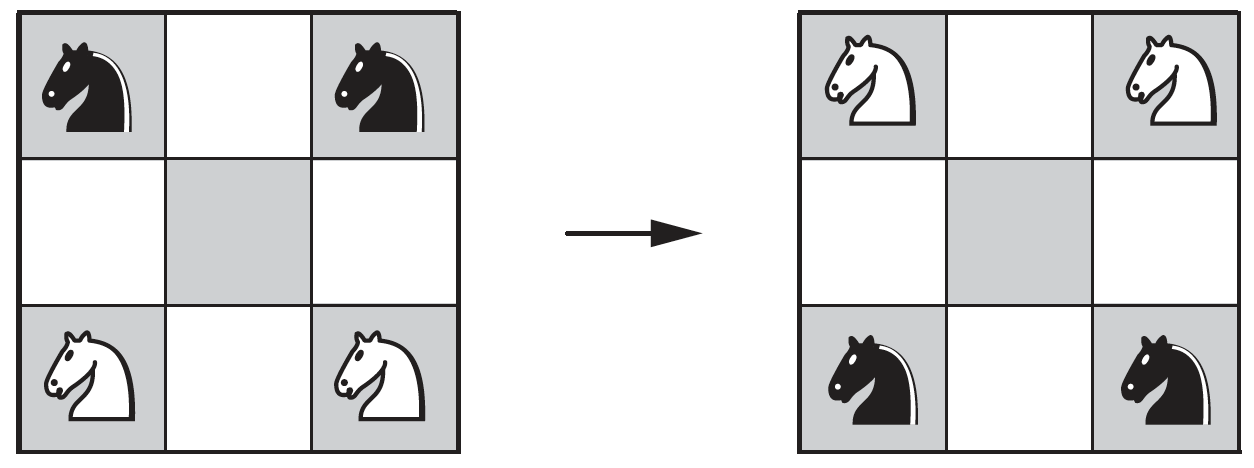
\includegraphics[width=8cm]{four_knights.png}%
\end{center}

\end{frame}

\ifanswers

\begin{frame}%[containsverbatim]
\frametitle{Solution}


%% There are four knights on the $3\times3$ chessboard: the two white knights
%% are at the two bottom corners, and the two black knights are at the two upper corners
%% of the board. The goal is to switch the knights in the minimum number of
%% moves so that the white knights are at the upper corners and the black knights are
%% at the bottom corners.

\vspace{-0.2cm}

\begin{center}
\includegraphics<1>[width=10.5cm]{four_knights_solution.pdf}%
\includegraphics<2>[width=10.5cm]{four_knights_solution_bis.pdf}%
\includegraphics<3>[width=10.5cm]{four_knights_solution1.pdf}%
\includegraphics<4>[width=10.5cm]{four_knights_solution2.pdf}%
\end{center}

\end{frame}

\fi

\begin{frame}%[containsverbatim]
\frametitle{Break the Problem Into Pieces}

Another approach is to break the problem into pieces.

\begin{itemize}

\vspace{0.2cm}

\item<1-> The hope is that each piece
is an easier problem, preferably a mere exercise.

\vspace{0.2cm}

\item<1-> Hence, divide the problem into as many
natural cases as is possible.

\end{itemize}

%\vspace{0.4cm}

%% Now consider the third problem; it involves natural numbers. The set of natural numbers
%% can be divided into two: even numbers and odd numbers. Let's look at the case of even
%% numbers, that is, $n = 2m$ for some natural number $m$. The equation becomes:\\
%% $$
%% x^2 + y^2 = z^{2m} = (z^m)^2
%% $$
%% Thus we have something of the form $x^2 + y^2 = w^2$ (where $w = z^m$). This looks like
%% the case where $n = 2$. Maybe we can use the solution we got in that case to help us.\\

\end{frame}

\begin{frame}%[containsverbatim]
\frametitle{Break the Problem Into Pieces}

\begin{center}
\includegraphics<1>[width=8cm]{polya_break.pdf}%
\includegraphics<2>[width=8cm]{polya_break1.pdf}%
\end{center}

%% Now consider the third problem; it involves natural numbers. The set of natural numbers
%% can be divided into two: even numbers and odd numbers. Let's look at the case of even
%% numbers, that is, $n = 2m$ for some natural number $m$. The equation becomes:\\
%% $$
%% x^2 + y^2 = z^{2m} = (z^m)^2
%% $$
%% Thus we have something of the form $x^2 + y^2 = w^2$ (where $w = z^m$). This looks like
%% the case where $n = 2$. Maybe we can use the solution we got in that case to help us.\\

\end{frame}

\subsection{Executing the Plan}

\begin{frame}%[containsverbatim]
\frametitle{Executing the Plan}

\begin{itemize}

\item Once the plan has been made, it needs to be carried out.
\begin{itemize}
\item<1-> By now you should have a good
idea of why a result is true, next work out precisely what convinced you and polish that.
\end{itemize}

\vspace{0.5cm}

\item<2-> Check each step carefully and ensure that it is justified.
\begin{itemize}
\item<2-> Any argument is only as strong as
its weakest link. If only one small step is incorrect, then the whole argument is false.
\end{itemize}
% Now
%is the time to avoid using intuition. If you think something is true, then prove it beyond
%doubt by using small steps of logic.

\end{itemize}

\end{frame}

\subsection{Looking Back}

\begin{frame}%[containsverbatim]
\frametitle{Looking Back}

Even though you have produced a solution, the problem-solving plan is not finished:
\vspace{0.3cm}
\begin{itemize}
\item<1-> Test your solution.
\vspace{0.5cm}
\item<1-> Reflect on what you have done.
\end{itemize}

\end{frame}

%% \begin{frame}[containsverbatim]
%% \frametitle{Check the Answer}

%% \textbf{Testing your answer is important}. First, does the answer make sense. Is it of the right
%% order? If you have calculated that your car is travelling at a million miles an hour, or that
%% the Sun is 299 km from the Earth, then it is unlikely that your answer is correct.\\

%% \vspace{0.4cm}

%% If you have at your disposal correct answers for a given set of data, test your solution on those data.\\

%% \vspace{0.4cm}

%% Simple tests are often available. For example:

%% \begin{itemize}

%% \item The angles in a triangle should add up to
%% 180 degrees.\\

%% \item Another simple test involves the idea of parity. This is easier to see in action
%% than give a good definition. The equation $51^2 = 34^2 + 46^2$ is false. This is easy to see
%% without any calculation: The left-hand side is odd and the right-hand side is even. That's
%% parity!

%% \end{itemize}

%% \end{frame}

%% \begin{frame}[containsverbatim]
%% \frametitle{Find Another Solution}

%% Even though a solution has been found there may be a better one, so attempt to \textbf{solve the
%% problem in a different way}.\\

%% \vspace{0.4cm}

%% \textbf{Compare yours with model solutions}, if they are available.

%% \end{frame}

\begin{frame}%[containsverbatim]
\frametitle{Reflect}

\setbeamercovered{transparent=0}

Reflection really pays in solving problems. Think about what solved the problem and ask
questions:
\begin{itemize}
\item<1-> How is the solution similar to others?\\
\item<1-> How is it different?\\
\item<1-> Was a certain theorem
or technique used and does it keep getting used?
\end{itemize}
\vspace{0.4cm}
\onslide<2->
As Descartes ($1596$-$1650$) said: ``Each problem that I solved became a rule, which served afterwards to solve other problems.''
%% Think about what keeps cropping up and
%% put it in your armoury, ready to attack future problems.

\end{frame}

\subsection{Exercices}

\begin{frame}%[containsverbatim]
\frametitle{Three Last Pieces of Advice}

\begin{itemize}

\item Do not give up too soon! Believe in yourself \dSmiley.

\vspace{0.5cm}

\item If you cannot solve a problem, remember that you solve a problem or you learn something new!

\vspace{0.5cm}

\item Solving problems should be fun, so do not put pressure on yourself or blame yourself
when you don't succeed.

\end{itemize}

\end{frame}

\begin{frame}%[containsverbatim]
\frametitle{\exo}

\footnotesize

\begin{mdframed}[style=exampledefault]
Problem: Consider the following diagram. Can you connect each small box on
the top with its same-letter mate on the bottom with paths that do not cross one another,
nor leave the boundaries of the large box?
\end{mdframed}

\begin{center}
\includegraphics<1>[width=6.1cm]{do_not_give_up.pdf}%
\end{center}

\end{frame}

\ifanswers

\begin{frame}%[containsverbatim]
\frametitle{Solution}

Solve an easier problem!

\begin{center}
\includegraphics<1>[width=7cm]{do_not_give_up_sol.pdf}%
\end{center}

\end{frame}

\begin{frame}%[containsverbatim]
\frametitle{Solution}

And work backward from there!

\begin{center}
\includegraphics<1>[width=7cm]{do_not_give_up_sol1.pdf}%
\includegraphics<2>[width=7cm]{do_not_give_up_sol2.pdf}%
\end{center}

\end{frame}


\fi

\begin{frame}[containsverbatim]
\frametitle{\exo}

%% Design a program to find the number of zeroes at the end of $n!$ where
%% $n$ can be as large as $10^9$.\\
%% \vspace{0.3cm}
%% If you solve this problem you can easily solve
\cheflink{Factorial}{https://www.codechef.com/problems/FCTRL}

\end{frame}

\ifanswers

\begin{frame}%[containsverbatim]
\frametitle{Solution}
\scriptsize

\begin{itemize}

\item<1-> Consider the factorial of $25$. We have
\begin{eqnarray*}
25! & = & 25\times24\times23\times22\times \cdots \times 10\times9\times8\times7\times6\times5\times4\times3\times2\times1\\
& = & (\textbf{5}\times\textbf{5}) \times 24 \times 23 \times 22 \times 21 \times (\textbf{5}\times4)\times19\times18\times17\times16 \times (\textbf{5}\times3) \times\\
&  & 14\times13\times12 \times 11 \times (\textbf{5}\times2)\times9\times8\times7\times6\times\textbf{5}\times4\times3\times2\times1\\
\end{eqnarray*}

\item<2-> So we have to count the multiple of $5$ in $25!$.
\vspace{0.2cm}

\item<2-> We see that each five numbers we have a multiple of $5$. But if we count only them, we forget the $5$ in $25$.
\vspace{0.2cm}

\item<2-> Therefore, there are $\lfloor\frac{25}{25}\rfloor + \lfloor\frac{25}{5}\rfloor = 6$ zeroes at the end of $25!$.
\vspace{0.2cm}

\item<3-> The same method applies for $1000!$:
\begin{itemize}
\scriptsize
\item There are $\lfloor\frac{1000}{625}\rfloor + \lfloor\frac{1000}{125}\rfloor + \lfloor\frac{1000}{25}\rfloor + \lfloor\frac{1000}{5}\rfloor = 249$ zeroes at the end of $1000!$.
\end{itemize}

\end{itemize}

\end{frame}

\begin{frame}[containsverbatim]
\frametitle{Solution Implementation}
\scriptsize

\begin{lstlisting}
int main(int argc, char *argv[])
{
  int N;
  cin >> N;
  for (int i = 0; i < N; ++i)
  {
    int v;
    cin >> v;
    int res = 0;
    int d = 5;
    while (v / d != 0)
    {
      res += v / d;
      d *= 5;
    }
    cout << res << endl;
  }
  return 0;
}
\end{lstlisting}

\end{frame}

\fi

\begin{frame}%[containsverbatim]
\frametitle{\exo}

Show that the equation $x^2 + y^2 = z^n$ has positive integer solutions for every $n = 1, 2, 3, \ldots$.

\end{frame}

\ifanswers

\begin{frame}%[containsverbatim]
\frametitle{Solution}
\scriptsize
\begin{itemize}

\item<1-> We already know how to solve it for $n = 1$ and $n = 2$:
\begin{itemize}
\scriptsize
\item<1-> $x^2 + y^2 = z$.
\item<1-> $x^2 + y^2 = z^2$ because of Pythagore.
\end{itemize}
%\vspace{0.35cm}
\item<2-> Let $n$ be odd, we must show that $x^2 + y^2 = z^{2k+1}$ (with $k \ge 0$).
\begin{itemize}
\scriptsize
\item<2-> We can work backward:
\begin{align*}
\onslide<2->{z^{2k+1}} & \onslide<2->{=} \onslide<2->{z^{2k}\times z\\}
\onslide<3->{z_1^{2k+1}} & \onslide<3->{=} \onslide<3->{z_1^{2k}\times (x_1^2 + y_1^2) \quad \textrm{($z_1 = x_1^2 + y_1^2$, basic case $n = 1$)}\\}
& \onslide<4->{=} \onslide<4->{z_1^{2k}\times x_1^2 + z_1^{2k}\times y_1^2\\}
& \onslide<5->{=} \onslide<5->{(z_1^k\times x_1)^2 + (z_1^k\times y_1)^2}
\end{align*}
\end{itemize}
\vspace{-0.2cm}
\item<6-> Let $n$ be even, we must show that $x^2 + y^2 = z^{2k}$ (with $k > 0$).
\begin{itemize}
\scriptsize
\item<6-> We can also work backward:
\begin{align*}
\onslide<6->{z^{2k}} & \onslide<6->{=} \onslide<6->{z^{2k-2}\times z^2\\}
\onslide<7->{z_2^{2k}} & \onslide<7->{=} \onslide<7->{z_2^{2k-2}\times (x_2^2 + y_2^2) \quad \textrm{($z_2^2 = x_2^2 + y_2^2$, basic case $n = 2$)}\\}
& \onslide<8->{=} \onslide<8->{z_2^{2k-2}\times x_2^2 + z_2^{2k-2}\times y_2^2\\}
& \onslide<9->{=} \onslide<9->{(z_2^{k-1}\times x_2)^2 + (z_2^{k-1}\times y_2)^2\\}
\end{align*}

\end{itemize}

\end{itemize}

\end{frame}

\fi

\begin{frame}%[containsverbatim]
\frametitle{\exo}

Prove that the product of four consecutive numbers in $\mathbb{N}^*$ cannot be
the square of an integer.

\end{frame}

\ifanswers

\begin{frame}%[containsverbatim]
\frametitle{Solution}

\scriptsize

\begin{itemize}

\item<1-> Let's write down a serie of four consecutive numbers:\\

\vspace{0.3cm}

\begin{tabular}{|c|c|c|c|c|}
\hline
$1\times2\times3\times4$ & $2\times3\times4\times5$ & $3\times4\times5\times6$ & $4\times5\times6\times7$ & $5\times6\times7\times8$\\
\hline
$24$ & $120$ & $360$ & $840$ & $1680$\\
\hline
\end{tabular}

\vspace{0.3cm}

\item<2-> Because the problem is related to squares, looking for a relation between the previous numbers
and squares, we find\\

\vspace{0.3cm}

\begin{tabular}{|c|c|c|c|c|}
\hline
$1\times2\times3\times4$ & $2\times3\times4\times5$ & $3\times4\times5\times6$ & $4\times5\times6\times7$ & $5\times6\times7\times8$\\
\hline
$5^2 - 1$ & $11^2 - 1$ & $19^2 - 1$ & $29^2 - 1$ & $41^2 - 1$\\
\hline
\end{tabular}
\vspace{0.3cm}

\item<3-> Now, if $n>0$, $n^2 - 1$ cannot be the square of an integer:
$$
(n+1)^2 = n^2 + 2n + 1 > n^2 + 1.
$$

\end{itemize}

\end{frame}

\begin{frame}%[containsverbatim]
\frametitle{Solution}

\setbeamercovered{transparent}

\scriptsize

\begin{itemize}

\item<cover> Because the problem is related to squares, looking for a relation between the previous numbers
and squares, we find\\

\vspace{0.3cm}

\begin{tabular}{|c|c|c|c|c|}
\hline
$1\times2\times3\times4$ & $2\times3\times4\times5$ & $3\times4\times5\times6$ & $4\times5\times6\times7$ & $5\times6\times7\times8$\\
\hline
$5^2 - 1$ & $11^2 - 1$ & $19^2 - 1$ & $29^2 - 1$ & $41^2 - 1$\\
\hline
\end{tabular}
\vspace{0.3cm}

\item<cover> Now, if $n>0$, $n^2 - 1$ cannot be the square of an integer: $(n+1)^2 = n^2 + 2n + 1 > n^2 + 1$.
\vspace{0.3cm}

\item<1-> To finish, we need to show that $n\times(n+1)\times(n+2)\times(n+3) = X^2 - 1$, for some integer $X$:

\begin{eqnarray*}
n\times(n+1)\times(n+2)\times(n+3) &=& n^4 + 6n^3 + 11n^2 + 6n\\
&=& (n^2 + an + b)^2 - 1 \quad \textrm{(we hope)}
\end{eqnarray*}

\onslide<2>
{\color<1>{white}
\begin{eqnarray*}
(n^2 + an + b)^2 - 1 &=& n^4 + 2an^3 + (a^2+2b)n^2 + 2abn + b^2 - 1\\
&=& (n^2 + 3n + 1)^2 -1 \quad \textrm{(by identification)}
\end{eqnarray*}
}
\end{itemize}

\end{frame}

\fi

\section{Proof Techniques}

\subsection{Proof by Induction}

\begin{frame}%[containsverbatim]
\frametitle{Proof by Induction}

We give in this part a review of mathematical induction because
\begin{itemize}

\item<1-> We will use a variation of this principle
to solve algorithmic problems (\emph{Design of Algorithms by Induction}).

\vspace{0.3cm}

\item<2-> For some problems, we have to guess a pattern for a given sequence, and we can prove
by induction that our guess is correct.

\end{itemize}

\end{frame}

%\subsection{Mathematical Induction}

\begin{frame}%[containsverbatim]
\frametitle{Mathematical Induction}

\begin{block}{Principle of Mathematical Induction}

Let \textcolor{blue}{$P(n)$} be a property that is defined for integers \textcolor{blue}{$n$}, and let \textcolor{blue}{$a$} be a fixed integer.
Suppose the following two statements are true:\\
\begin{enumerate}
\item<2-> $P(a)$ is true.\\

\item<2-> For all integers $k \ge a$, if $P(k)$ is true then $P(k+1)$ is true.
\end{enumerate}

\onslide<3->
Then the statement
\begin{center}
For all integers $n \ge a$, $P(n)$
\end{center}
is also true.
\end{block}

\end{frame}

\begin{frame}%[containsverbatim]
\frametitle{Method of Proof by Mathematical Induction}
\footnotesize

\begin{block}{Method of Proof by Mathematical Induction}
Consider a statement of the form:\\
\hspace{1cm} ``For all integers $n \ge a$, a property $P(n)$ is true.''\\
\vspace{0.1cm}
To prove such a statement, perform the following two steps:\\
\begin{itemize}

\item<1-> \textcolor{blue}{Step 1 (basic step):} Show that $P(a)$ is true.\\
\vspace{0.2cm}
\item<1-> \textcolor{blue}{Step 2 (inductive step):} Show that for all integers $k \ge a$, if $P(k)$ is true then
$P(k+1)$ is true. To perform this step,\\
\vspace{0.2cm}
\onslide<2->
\begin{center}
\textbf{Suppose} that $P(k)$ is true where $k$ is any arbitrarily chosen integer with $k \ge a$.\\
\scriptsize
$[$\emph{This supposition is called the} \textbf{inductive hypothesis}.$]$
\normalsize
\end{center}
\vspace{0.2cm}
%\onslide<3->
Then
\begin{center}
\textbf{Show} that $P(k + 1)$ is true.
\end{center}

\end{itemize}
\end{block}

\end{frame}


\begin{frame}%[containsverbatim]
\frametitle{Example}

\setbeamercovered{transparent=0}

\scriptsize

\begin{block}{}
For all integers $n \ge 8$, $n$ cents can be obtained using $3$ cents and $5$ cents coins.
\end{block}
\onslide<2->
\textcolor{blue}{Proof (by mathematical induction).}\\
\vspace{0.15cm}
Let the property $P(n)$ be the sentence\\
\begin{center}
\framebox{$n$ cents can be obtained using $3$ cents and $5$ cents coins.}
\end{center}
\begin{enumerate}
\item<3-> \textbf{Show that $P(8)$ is true.} $P(8)$ is true because $8$ cents can be obtained using one $3$ cents coin and one $5$ cents coin.\\

\vspace{0.2cm}

\item<4-> \textbf{Show that for all integers $k \ge 8$, if $P(k)$ is true then $P(k+1)$ is also true.}\\
%\onslide<5->
Suppose that $k$ is any integer with $k \ge 8$ such that\\
\begin{center}
$k$ cents can be obtained using $3$ cents and $5$ cents coins.
\end{center}
%\onslide<6->
We must show that\\
\begin{center}
$(k + 1)$ cents can be obtained using $3$ cents and $5$ cents coins.
\end{center}

\end{enumerate}

\end{frame}

\begin{frame}%[containsverbatim]
\frametitle{Example}

\setbeamercovered{transparent=0}

\scriptsize

\begin{block}{}
For all integers $n \ge 8$, $n$ cents can be obtained using $3$ cents and $5$ cents coins.
\end{block}

\begin{enumerate}
\setcounter{enumi}{1}
\item \textbf{Show that for all integers $k \ge 8$, if $P(k)$ is true then $P(k+1)$ is also true:}\\
\vspace{0.2cm}
\begin{itemize}
\scriptsize
\item<2-> \textbf{Case 1.} There is a $5$ cents coin among those used to make up the $k$ cents.
\begin{center}
\includegraphics<3>[width=7cm]{coins_induction.pdf}%
\includegraphics<4>[width=7cm]{coins_induction1.pdf}%
\end{center}


%%  In this
%% case, replace the $5$ cents coin by two $3$ cents coins; the result will be $(k+1)$ cents.\\
\item<5-> \textbf{Case 2.} There is not a $5$ cents coin among those used to make up the $k$ cents.
\begin{overlayarea}{1\textwidth}{0.5\textheight}
\begin{center}
\includegraphics<6>[width=7cm]{coins_induction2.pdf}%
\includegraphics<7>[width=7cm]{coins_induction3.pdf}%
\end{center}
\end{overlayarea}
%% In this
%% case, because $k \ge 8$, at least three $3$ cents coins must have been used. So remove three $3$ cents coins
%% and replace them by two $5$ cents coins; the result will be $(k+1)$ cents.

\end{itemize}

\end{enumerate}

\end{frame}

\begin{frame}%[containsverbatim]
\frametitle{Wrong Usage}

\setbeamercovered{transparent=0}

\footnotesize

We will \textbf{incorrectly} prove by induction that in any sequence of real numbers, all elements are equal!
\begin{block}{}
In any sequence of real numbers, all elements are equal.
\end{block}
\onslide<2->
\textcolor{blue}{Incorrect Proof (by mathematical induction).}\\
\vspace{0.15cm}
Let the property $P(n)$ be the sentence\\
\begin{center}
\framebox{For any real numbers $a_1$, $a_2$, \ldots, $a_n$, we have $a_1 = a_2 = \ldots = a_n$.}
\end{center}

\begin{itemize}

\item<3-> \textbf{Show that $P(1)$ is true.} Indeed the sequence contains only one real number.

\end{itemize}


\end{frame}

\begin{frame}%[containsverbatim]
\frametitle{Wrong Usage}

\setbeamercovered{transparent=0}

\scriptsize

\begin{itemize}

\item \textbf{Show that for all integers $k \ge 1$, if $P(k)$ is true then $P(k+1)$ is also true.}\\
\vspace{0.2cm}

\onslide<2->
Suppose that $k$ is any integer with $k \ge 1$ such that $P(k)$ is true (i.e., that any $k$ real numbers must be equal).\\
%% We seek
%% to show that $P(k+1)$ is true as well, i.e., any $k+1$ real numbers must also be equal.\\

\onslide<3->
\vspace{0.2cm}
Let $a_1$, $a_2$, \ldots, $a_{k+1}$ be given real numbers. Applying the induction hypothesis to the first $k$
of these numbers, $a_1$, $a_2$, \ldots, $a_k$, we obtain\\
\onslide<3->
$$
a_1 = a_2 = \ldots = a_k \qquad (1)
$$
\onslide<4->
Similarly, applying the induction hypothesis to the last $k$ of these numbers, $a_2$, $a_3$, \ldots, $a_k$, $a_{k+1}$, we get\\
$$
a_2 = a_3 = \ldots = a_k = a_{k+1} \qquad (2)
$$
\onslide<5->
Combining (1) and (2) gives\\
$$
a_1 = a_2 = \ldots = a_k = a_{k+1} \qquad (3)
$$

Thus we have proved $P(k+1)$.

\end{itemize}

\end{frame}

\begin{frame}%[containsverbatim]
\frametitle{\exo}

What is wrong with the preceding proof?

\end{frame}

\ifanswers

\begin{frame}%[containsverbatim]
\frametitle{Solution}

When $n = 2$, our line of reasoning breaks down. You cannot have $a_1 = a_2 = \ldots = a_k$ and $a_2 = a_3 = \ldots = a_{k+1}$.

\end{frame}

\fi

\begin{frame}%[containsverbatim]
\frametitle{\exo}
\scriptsize
Prove by induction that
\begin{block}{}
For all $n \ge 3$, if $n$ distinct points on a circle are connected in consecutive order by straight lines, then the
interior angles of the resulting polygon add up to: $(n-2)180$\textdegree.
\end{block}
\vspace{0.2cm}

For example, with $n = 4$

\begin{overlayarea}{1\textwidth}{0.6\textheight}
\begin{center}
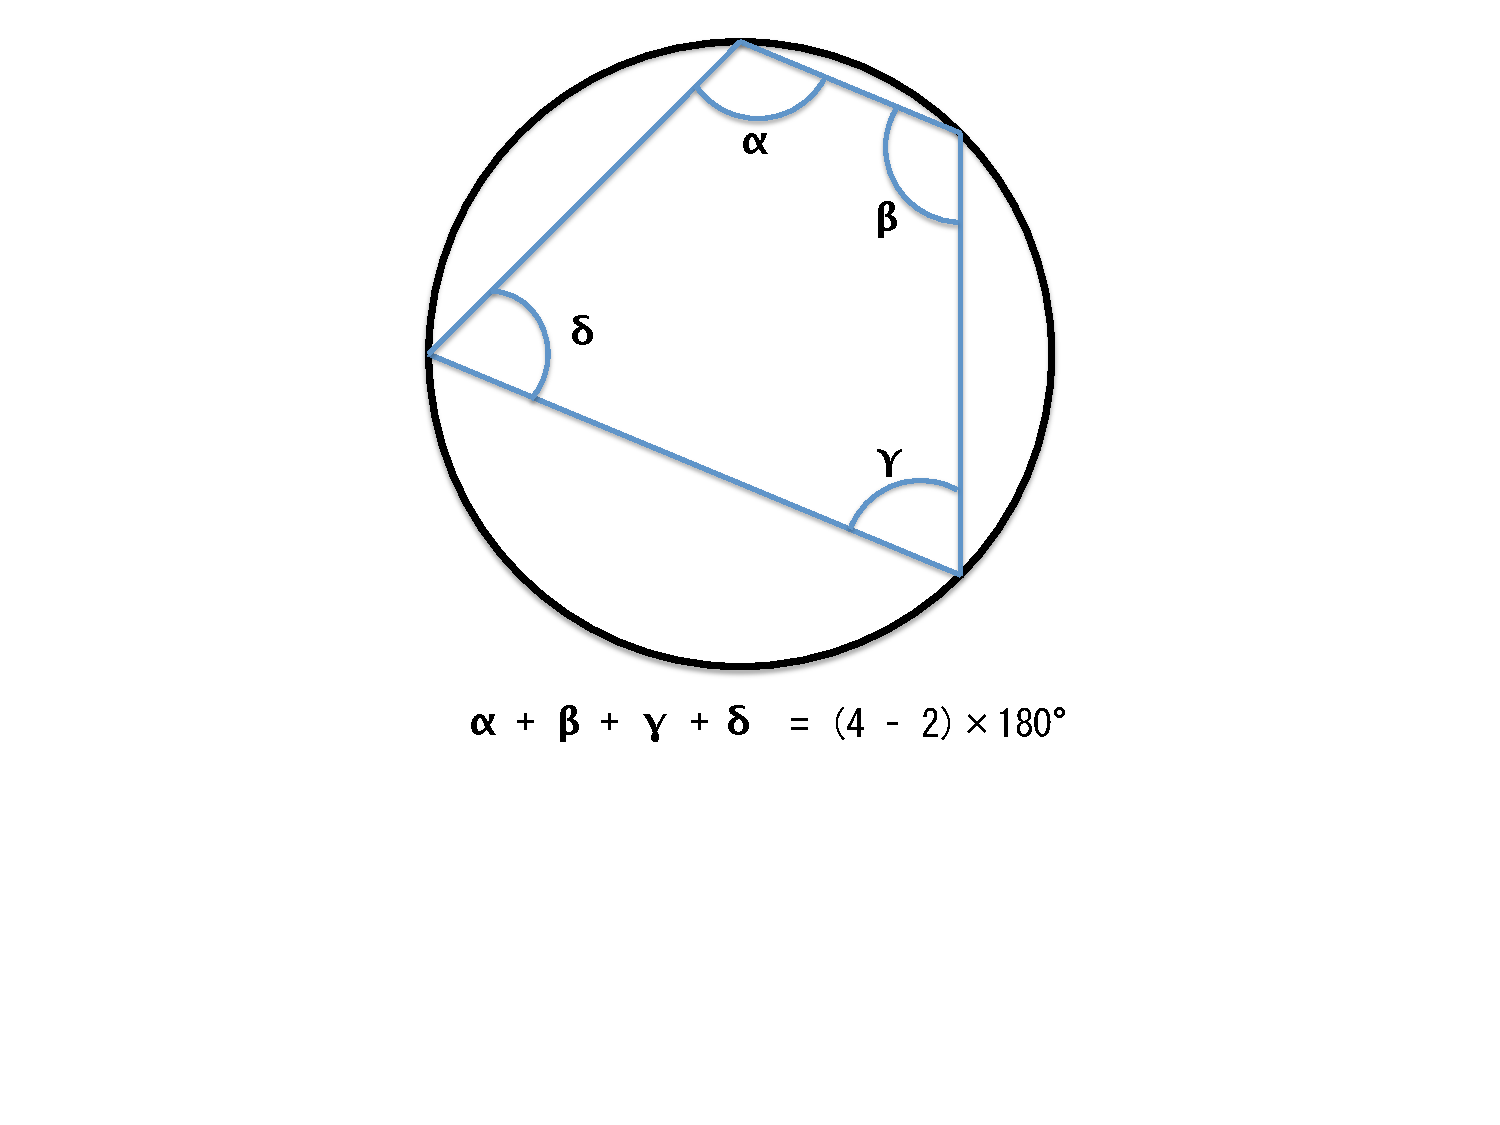
\includegraphics[width=9cm]{induction_circle.pdf}%
\end{center}
\end{overlayarea}

\end{frame}

\ifanswers

\begin{frame}%[containsverbatim]
\frametitle{Solution}

\scriptsize

\begin{itemize}

\item \textbf{Base case:} $n = 3$, so the shape is reduced to a triangle whose angles sum to $180$\textdegree.

\vspace{0.3cm}

\item<2-> \textbf{Inductive case:} We know how to prove it for $k$ points, how to prove it for $(k+1)$?

\begin{overlayarea}{1\textwidth}{0.6\textheight}
\begin{center}
\includegraphics<3>[width=6cm]{induction_circle1.pdf}%
\includegraphics<4>[width=6cm]{induction_circle2.pdf}%
%\includegraphics<5>[width=6cm]{induction_circle3.pdf}%
\includegraphics<5>[width=6cm]{induction_circle4.pdf}%
\includegraphics<6>[width=6cm]{induction_circle5.pdf}%
\includegraphics<7>[width=6cm]{induction_circle6.pdf}%
\includegraphics<8>[width=6cm]{induction_circle7.pdf}%
\end{center}
\end{overlayarea}

\end{itemize}

\end{frame}

\fi

\begin{frame}%[containsverbatim]
\frametitle{\exo}

\scriptsize

Prove by induction that
\begin{block}{}
For any integer $n \ge 0$, a $2^n \times 2^n$ square grid with any one square removed can be covered with L-shaped tiles that look like:
\begin{center}
$\boxplus$ with any one square removed.
\end{center}
\end{block}
\vspace{0.3cm}

For example, with $n = 3$, we could have the following grid:\\

\vspace{0.5cm}

\begin{overlayarea}{1\textwidth}{0.6\textheight}
\begin{center}
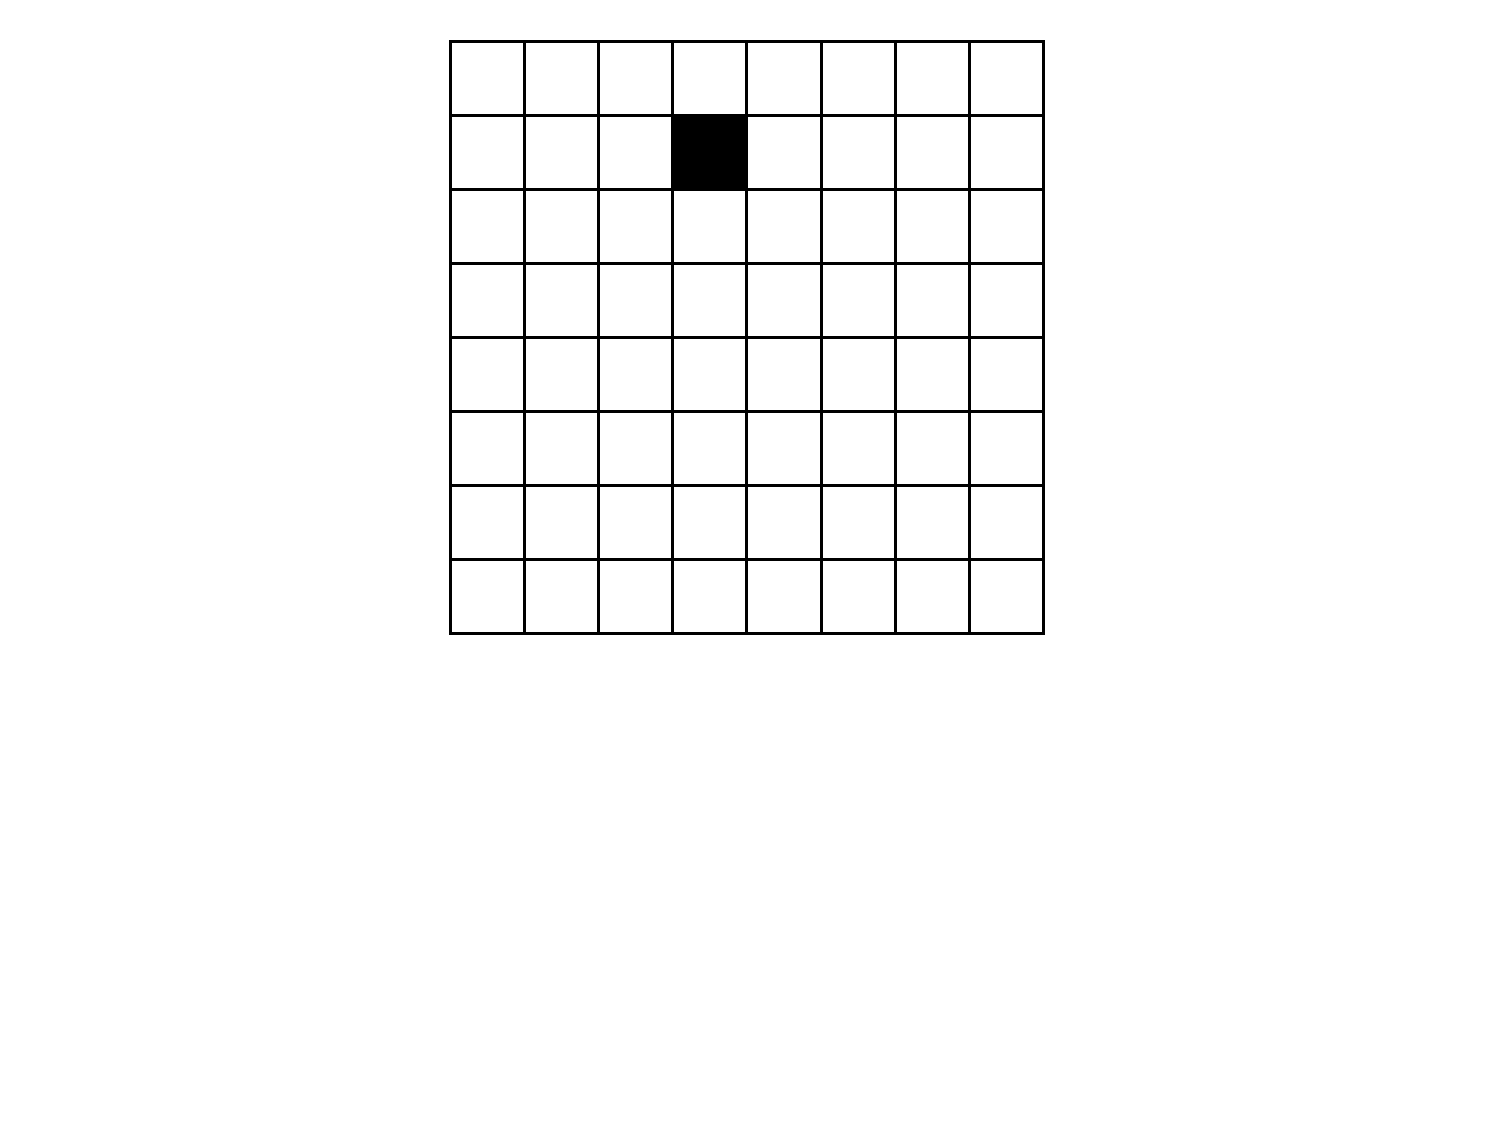
\includegraphics[width=7cm]{induction_Lshaped_tiles.pdf}%
\end{center}
\end{overlayarea}

\end{frame}

\ifanswers

\begin{frame}%[containsverbatim]
\frametitle{Solution}

\scriptsize

\begin{itemize}

\item \textbf{Base case:} $n = 0$, so we have a grid of dimension $1\times1$ with one filled square. There is nothing to do!

\vspace{0.3cm}

\item<2-> \textbf{Inductive case:} we know how to solve it for $k$ ($2^k\times2^k$ square), how to do it for $(k+1)$?

\begin{overlayarea}{1\textwidth}{0.7\textheight}
\vspace{-0.5cm}
\begin{center}
\includegraphics<3>[width=7cm]{induction_Lshaped_tiles1.pdf}%
\includegraphics<4>[width=7cm]{induction_Lshaped_tiles2.pdf}%
\includegraphics<5>[width=7cm]{induction_Lshaped_tiles3.pdf}%
\includegraphics<6>[width=7cm]{induction_Lshaped_tiles4.pdf}%
\includegraphics<7>[width=7cm]{induction_Lshaped_tiles5.pdf}%
\includegraphics<8>[width=7cm]{induction_Lshaped_tiles6.pdf}%
\includegraphics<9>[width=7cm]{induction_Lshaped_tiles7.pdf}%
\includegraphics<10>[width=7cm]{induction_Lshaped_tiles8.pdf}%
\includegraphics<11>[width=7cm]{induction_Lshaped_tiles9.pdf}%
\includegraphics<12>[width=7cm]{induction_Lshaped_tiles10.pdf}%
\end{center}
\end{overlayarea}


\end{itemize}


\end{frame}

\fi

%\subsection{Strong Mathematical Induction}

\begin{frame}%[containsverbatim]
\frametitle{Strong Mathematical Induction}

\footnotesize

\begin{block}{Principle of Strong Mathematical Induction}

Let \textcolor{blue}{$P(n)$} be a property that is defined for integers \textcolor{blue}{$n$}, and let \textcolor{blue}{$a$} and \textcolor{blue}{$b$}
be fixed integers with \textcolor{blue}{$a \le b$}.
Suppose the following two statements are true:\\
\begin{enumerate}
\item<2-> $P(a), P(a+1), \ldots, P(b)$ are all true.\\

\item<2-> For any integers $k \ge b$, if $P(i)$ is true for all $i$ from $a$ through $k$, then $P(k+1)$ is true.\\
\end{enumerate}
\onslide<3->
Then the statement:
\begin{center}
For all integers $n \ge a$, $P(n)$
\end{center}
is true.
\end{block}
\vspace{0.3cm}
\onslide<4->
\textbf{Note:} The principles of induction and strong induction are equivalent.

\end{frame}

\begin{frame}%[containsverbatim]
\frametitle{Example: Nim Game}

\begin{center}
\includegraphics<1>[width=7cm]{nim_game.pdf}%
\includegraphics<2>[width=7cm]{nim_game1.pdf}%
\includegraphics<3>[width=7cm]{nim_game2.pdf}%
\includegraphics<4>[width=7cm]{nim_game3.pdf}%
\includegraphics<5>[width=7cm]{nim_game4.pdf}%
\includegraphics<6>[width=7cm]{nim_game5.pdf}%
\includegraphics<7>[width=7cm]{nim_game6.pdf}%
\includegraphics<8>[width=7cm]{nim_game7.pdf}%
\includegraphics<9>[width=7cm]{nim_game7bis.pdf}%
\includegraphics<10>[width=7cm]{nim_game8.pdf}%
\includegraphics<11>[width=7cm]{nim_game9.pdf}%
\includegraphics<12>[width=7cm]{nim_game10.pdf}%
\includegraphics<13>[width=7cm]{nim_game11.pdf}%
\includegraphics<14>[width=7cm]{nim_game12.pdf}%
\includegraphics<15>[width=7cm]{nim_game13.pdf}%
\includegraphics<16>[width=7cm]{nim_game14.pdf}%
\includegraphics<17>[width=7cm]{nim_game15.pdf}%
\end{center}

\end{frame}

\begin{frame}%[containsverbatim]
\frametitle{Example: Nim Game}

\begin{block}{Definition}
Let $x = (x_m \ldots x_0)_2 \in \mathbb{N}$ and $y = (y_m \ldots y_0)_2 \in \mathbb{N}$. Then, $x \oplus y = (z_m \ldots z_0)_2$
with \begin{tabular}{|c|c||c|}
\hline
$x_k$ & $y_k$ & $z_k$\\
\hline
0 & 0 & 0\\
0 & 1 & 1\\
1 & 0 & 1\\
1 & 1 & 0\\
\hline
\end{tabular}
\end{block}

\vspace{0.4cm}

\onslide<2->

\begin{block}{Theorem} A \emph{nim} position $(x,y,z)$ is a winning position \emph{iff}
$x \oplus y \oplus z \ne 0$. A \emph{nim} position $(x,y,z)$ is a losing one \emph{iff}
$x \oplus y \oplus z = 0$.
\end{block}

\end{frame}

\begin{frame}%[containsverbatim]
\frametitle{Example: Nim Game}

\scriptsize

\begin{itemize}

\item $P(n)$: The positions $(n_1, n_2, n_3)$ with $n = n_1 + n_2 + n_3$ are
\begin{itemize}
\scriptsize
\item<1-> Losing positions \emph{iff} $n_1 \oplus n_2 \oplus n_3 = 0$.
\item<1-> Winning positions \emph{iff} $n_1 \oplus n_2 \oplus n_3 \ne 0$.
\end{itemize}

\vspace{0.2cm}

\item<2-> We prove by strong induction on $n$ that this property is true for all $n$.

\vspace{0.2cm}

\item<3-> \textbf{Base case:} $n = 0$, the only position is $(0, 0, 0)$. It is a losing position and we have $0 \oplus 0 \oplus 0 = 0$.

\vspace{0.2cm}

\item<4-> \textbf{Inductive case:} Let $n > 0$ and suppose that the property is true for all $k < n$. Let $n = n_1 + n_2 + n_3$.
\begin{itemize}
\scriptsize
\item<4-> \textbf{First case:} $n_1 \oplus n_2 \oplus n_3 = 0$.
\begin{itemize}
\item<5-> Any move in this position will change one of the $n_i > 0$, let's say $n_1$, into $n_1'$ with $n_1' < n_1$.
\item<6-> We have $n_1' \oplus n_2 \oplus n_3 \ne 0$. Otherwise, we would have $n_1' \oplus n_2 \oplus n_3 = 0 = n_1 \oplus n_2 \oplus n_3$ and
therefore $n_1 = n_1'$.
\item<7-> By the induction hypothesis, $(n_1', n_2, n_3)$ is a winning position.
\item<8-> Therefore $(n_1, n_2, n_3)$ is a losing position, because all legal moves lead to a winning position.

\end{itemize}

\end{itemize}

\end{itemize}

\end{frame}


\begin{frame}%[containsverbatim]
\frametitle{Example: Nim Game}

\scriptsize

\begin{itemize}

\item \textbf{Inductive case:} Let $n > 0$ and suppose that the property is true for all $k < n$. Let $n = n_1 + n_2 + n_3$.
\begin{itemize}
\scriptsize
\item \textbf{Second case:} $n_1 \oplus n_2 \oplus n_3 \ne 0$.
\begin{overlayarea}{0.5\textwidth}{0.55\textheight}
\begin{center}
\vspace{-0.28cm}
\includegraphics<2>[width=5cm]{nim_game16.pdf}%
\includegraphics<3>[width=5cm]{nim_game17.pdf}%
\includegraphics<4>[width=5cm]{nim_game18.pdf}%
\includegraphics<5>[width=5cm]{nim_game19.pdf}%
\includegraphics<6>[width=5cm]{nim_game20.pdf}%
\includegraphics<7>[width=5cm]{nim_game21.pdf}%
\includegraphics<8>[width=5cm]{nim_game22.pdf}%
\includegraphics<9->[width=5cm]{nim_game23.pdf}%
\end{center}
\end{overlayarea}
\vspace{-1cm}
\begin{itemize}
\scriptsize
\item<10-> Therefore, we can reach a position $(n_1', n_2', n_3')$ where $n_1' + n_2' + n_3' = k < n$ and
$n_1' \oplus n_2' \oplus n_3' = 0$.
\vspace{0.2cm}
\item<11> By the inductive hypothesis, $(n_1', n_2', n_3')$ is a losing position and so $(n_1, n_2, n_3)$ is a winning one because
we have a winning move in this position.
\end{itemize}

\end{itemize}

\end{itemize}

\end{frame}




\begin{frame}[containsverbatim]
\frametitle{\exo}

Consider the following sequence:

\[ s_n = \left\{
  \begin{array}{l l}
    0 & \quad \text{if $n = 0$}\\
    4 & \quad \text{if $n = 1$}\\
    6s_{n-1} - 5s_{n-2} & \quad \text{else}
  \end{array} \right.\]

\begin{enumerate}
\item Find the first five terms of this sequence.\\
\vspace{0.2cm}
\item Guess a closed-form solution for this sequence and prove by strong induction that your
guess is correct.
\end{enumerate}

\end{frame}

\ifanswers

\begin{frame}%[containsverbatim]
\frametitle{Solution}

\begin{itemize}
\item The first four terms are: $0$, $4$, $24$, $124$, $624$.
\vspace{0.2cm}
\item<2-> The Guessed closed-form is: $5^n - 1$.
\vspace{0.2cm}
\item<3-> \textbf{Base cases:} $5^0 - 1 = 0$ and $5^1 - 1 = 4$.
\vspace{0.2cm}
\item<4-> \textbf{Inductive case:} Suppose the closed form is true for all $k < n$.
\begin{align*}
\onslide<5->{s_n} & \onslide<5->{=} \onslide<5->{6s_{n-1} - 5s_{n-2}\\}
& \onslide<6->{=} \onslide<6->{6\times(5^{n-1} - 1) - 5\times(5^{n-2} - 1)\\}
& \onslide<7->{=} \onslide<7->{6\times5^{n-1} - 6 - 5^{n-1} + 5\\}
& \onslide<8->{=} \onslide<8->{5^{n-1}\times(6 - 1) - 1\\}
& \onslide<9->{=} \onslide<9->{5^n - 1}
\end{align*}
\end{itemize}

\end{frame}

\fi

\begin{frame}[containsverbatim]
\frametitle{\exo}

Unstacking game. TO DO

\end{frame}


\begin{frame}[containsverbatim]
\frametitle{\exo}

Solve \cheflink{Yet Another Number Game}{https://www.codechef.com/problems/NUMGAME/} Try to find a pattern and use induction to show that
this pattern is correct.\\
\vspace{0.2cm}
or\\
\vspace{0.2cm}
Solve \uvalink{12293}{https://uva.onlinejudge.org/index.php?option=com_onlinejudge&Itemid=8&category=24&page=show_problem&problem=3714}
Try to find a pattern and use induction to show that this pattern is correct.

\end{frame}

\ifanswers

\begin{frame}%[containsverbatim]
\frametitle{Yet Another Number Game Solution}
\scriptsize

\begin{itemize}

\item Let's follow Polya's advice and test the first few games. We get\\
\begin{center}
\begin{tabular}{|c|c|c|c|c|c|c|c|}
\hline
1 & 2 & 3 & 4 & 5 & 6 & 7 & 8\\
\hline
B & A & B & A & B & A & B & A\\
\hline
\end{tabular}
\end{center}

\item<2-> It seems that Alice wins when $N$ is even and Bob wins when $N$ is odd.

\vspace{0.2cm}

\item<3-> $P(n)$: The first player wins \emph{iff} $n$ is even.

\vspace{0.2cm}

\item<4-> \textbf{Base case:} It is true for $n = 1$.

\vspace{0.2cm}

\item<5-> \textbf{Inductive case:} Suppose that $P$ is true for all $k < n$:

\begin{itemize}
\scriptsize

\item<5-> If $n > 1$ is even, we just need to substract $1$ to get an odd number. Therefore we can reach
a losing position for the second player, and so the first player wins.

\vspace{0.1cm}

\item<6-> If $n > 1$ is odd. Every divisor of $n$ is odd.
\onslide<7->
Otherwise, if $d_1$ is an even divisor of $n$, we would have $n = d_1 \times d_2 = 2k \times d_2$. And $n$ would be even.\\
\onslide<8->
But odd minus odd is even ($2k + 1 - (2k' + 1) = 2(k - k')$), therefore we can only reach winning positions for the second player.
\end{itemize}

\end{itemize}

\end{frame}

\begin{frame}[containsverbatim]
\frametitle{Yet Another Number Game Implementation}
\scriptsize

\begin{lstlisting}
int main(int argc, char *argv[])
{
  int TC, N;
  cin >> TC;
  while (TC--)
  {
    cin >> N;
    if (N % 2) cout << "BOB";
    else cout << "ALICE";
    cout << endl;
  }
  return 0;
}
\end{lstlisting}

\end{frame}

\begin{frame}%[containsverbatim]
\frametitle{12293 Solution}

\begin{overlayarea}{1.2\textwidth}{1\textheight}
\begin{center}
\includegraphics<1>[width=7cm]{uva12293.pdf}%
\includegraphics<2>[width=7cm]{uva12293_1.pdf}%
\includegraphics<3>[width=7cm]{uva12293_2.pdf}%
\includegraphics<4>[width=7cm]{uva12293_3.pdf}%
\includegraphics<5>[width=7cm]{uva12293_4.pdf}%
\includegraphics<6>[width=7cm]{uva12293_5.pdf}%
\includegraphics<7>[width=7cm]{uva12293_6.pdf}%
\includegraphics<8>[width=7cm]{uva12293_7.pdf}%
\includegraphics<9>[width=7cm]{uva12293_8.pdf}%
\includegraphics<10>[width=7cm]{uva12293_9.pdf}%
\includegraphics<11>[width=7cm]{uva12293_10.pdf}%
\includegraphics<12>[width=7cm]{uva12293_11.pdf}%
\includegraphics<13>[width=7cm]{uva12293_12.pdf}%
\includegraphics<14>[width=7cm]{uva12293_13.pdf}%
\includegraphics<15>[width=7cm]{uva12293_14.pdf}%
\includegraphics<16>[width=7cm]{uva12293_15.pdf}%
\includegraphics<17>[width=7cm]{uva12293_16.pdf}%
\includegraphics<18>[width=7cm]{uva12293_17.pdf}%
\includegraphics<19>[width=7cm]{uva12293_18.pdf}%
\includegraphics<20>[width=7cm]{uva12293_19.pdf}%
\includegraphics<21>[width=7cm]{uva12293_20.pdf}%
\includegraphics<22>[width=7cm]{uva12293_21.pdf}%
\includegraphics<23>[width=7cm]{uva12293_22.pdf}%
\hspace{-2cm}\includegraphics<24>[width=10cm]{uva12293_23.pdf}%
\end{center}
\end{overlayarea}

\end{frame}

\begin{frame}%[containsverbatim]
\frametitle{12293 Solution}
\scriptsize

\begin{itemize}

\item It seems that the first player loses when $(n + 1)$ is a power of two.

\vspace{0.2cm}

\item<2-> $P(n)$: The first player loses \emph{iff} $(n + 1)$ is a power of two.

\vspace{0.2cm}

\item<3-> \textbf{Base case:} It is true for $n = 1$.

\vspace{0.2cm}

\item<4-> \textbf{Inductive case:} Suppose that $P$ is true for all $k < n$:

\begin{itemize}
\scriptsize

\item<4-> If $(n + 1)$ is a power of two, $n$ contains only ones in binary form (for example \texttt{11111}).
\onslide<5-> We cannot reach a number
with only ones in binary form (a losing state) from it.
\onslide<6->
Indeed, the biggest one we can get is \texttt{1111} because \texttt{11111 = 10000 + 1111} and \texttt{10000} is bigger than
\texttt{1111}.

\vspace{0.1cm}

\item<7-> If $(n + 1)$ is not a power of two, $n$ does not contain only ones in binary form (for example \texttt{10110}).
\onslide<8->
We can reach a number with only ones in binary form. Indeed, we can choose \texttt{1111}, and the other number will be strictly
less than \texttt{10000}.

\end{itemize}

\end{itemize}

\end{frame}

\begin{frame}[containsverbatim]
\frametitle{12293 Implementation}
\scriptsize

\begin{lstlisting}
int main(int argc, char *argv[])
{
  int n;
  string res[] = { "Alice", "Bob" };
  while (cin >> n, n)
  {
    ++n;
    cout << res[(n & (n - 1)) == 0] << endl;
  }
  return 0;
}
\end{lstlisting}

\end{frame}

\begin{frame}%[containsverbatim]
\frametitle{12293 Implementation}
\scriptsize

\begin{itemize}
\item $N =$ \texttt{10000}.\\
\begin{center}
\begin{tabular}{ll}
& \texttt{10000}\\
\texttt{\&} & \texttt{01111}\\
\hline
$=$ & \texttt{00000}\\
\end{tabular}
\end{center}

\vspace{0.2cm}

\item<2-> $N =$ \texttt{10100}.\\
\begin{center}
\begin{tabular}{ll}
& \texttt{10100}\\
\texttt{\&} & \texttt{10011}\\
\hline
$=$ & \texttt{10000}\\
\end{tabular}
\end{center}

\vspace{0.2cm}

\item<3-> $N =$ \texttt{10111}.\\
\begin{center}
\begin{tabular}{ll}
& \texttt{10111}\\
\texttt{\&} & \texttt{10110}\\
\hline
$=$ & \texttt{10110}\\
\end{tabular}
\end{center}

\end{itemize}

\end{frame}

\fi

\subsection{Inclusion-Exclusion Principle}

\begin{frame}%[containsverbatim]
\frametitle{Inclusion-Exclusion Principle}

\setbeamercovered{transparent=0}

The inclusion-exclusion principle  is a generalization of the rule
$$
|X\cup Y| = |X| + |Y| - |X\cap Y|,
$$
where $X$ and $Y$ are finite sets.

\begin{overlayarea}{1\textwidth}{0.6\textheight}
\begin{center}
\includegraphics<2>[width=7cm]{inclusion_exclusion_principle.pdf}%
\end{center}
\end{overlayarea}

\end{frame}

\begin{frame}%[containsverbatim]
\frametitle{Inclusion-Exclusion Principle}
\scriptsize
\begin{block}{Theorem (Inclusion-exclusion principle)}
Suppose that $A_1$, \ldots, $A_n$ are subsets of a finite set $S$. For $1 \le k \le n$, define
$$
I_{n,k} = \sum_{1 \le i_1 < \cdots < i_k \le n} |A_{i_1} \cap \cdots \cap A_{i_k}|.
$$
%\onslide<2->
Then
$$
|A_1 \cup \cdots \cup A_n| = \sum_{k = 1}^n (-1)^{k+1}I_{n,k}.
$$
\end{block}

%\onslide<3->

For example, with $A_1$, $A_2$ and $A_3$ we get
$$
I_{3,1} = |A_1| + |A_2| + |A_3|, \quad I_{3,2} = |A_1 \cap A_2| + |A_1 \cap A_3| + |A_2 \cap A_3|, \quad I_{3,3} = |A_1 \cap A_2 \cap A_3|.
$$

\onslide<2->
\vspace{0.2cm}
and finally,
$$
|A_1\cup A_2\cup A_3| = |A_1| + |A_2| + |A_3| - |A_1 \cap A_2| - |A_1 \cap A_3| - |A_2 \cap A_3| + |A_1 \cap A_2 \cap A_3|.
$$
\end{frame}

\begin{frame}%[containsverbatim]
\frametitle{Inclusion-Exclusion Principle}

\begin{center}
\includegraphics<1>[width=11cm]{inclusion_exclusion_principle1.pdf}%
\includegraphics<2>[width=11cm]{inclusion_exclusion_principle2.pdf}%
\includegraphics<3>[width=11cm]{inclusion_exclusion_principle3.pdf}%
\includegraphics<4>[width=11cm]{inclusion_exclusion_principle4.pdf}%
\includegraphics<5>[width=11cm]{inclusion_exclusion_principle5.pdf}%
\includegraphics<6>[width=11cm]{inclusion_exclusion_principle6.pdf}%
\includegraphics<7>[width=11cm]{inclusion_exclusion_principle7.pdf}%
\includegraphics<8>[width=11cm]{inclusion_exclusion_principle8.pdf}%
\includegraphics<9>[width=11cm]{inclusion_exclusion_principle9.pdf}%
\end{center}

\end{frame}

\begin{frame}%[containsverbatim]
\frametitle{Example}

\scriptsize

\begin{mdframed}[style=exampledefault]
Problem: How many positive integers less than or equal to $1000$ do not have $2$, $3$, or $5$ among their
prime factors?
\end{mdframed}

\begin{itemize}

\item<2-> Let $A_2$ be the number of multiples of $2$ less than $1000$. $A_2 = \lfloor\frac{1000}{2}\rfloor = 500$.

\item<3-> Let $A_3$ be the number of multiples of $3$ less than $1000$. $A_3 = \lfloor\frac{1000}{3}\rfloor = 333$.

\item<4-> Let $A_5$ be the number of multiples of $5$ less than $1000$. $A_5 = \lfloor\frac{1000}{5}\rfloor = 200$.

\item<5-> Let $A_{6}$ be the number of multiples of $6$ less than $1000$. $A_6 = \lfloor\frac{1000}{6}\rfloor = 166$.

\item<6-> Let $A_{10}$ be the number of multiples of $10$ less than $1000$. $A_{10} = \lfloor\frac{1000}{10}\rfloor = 100$.

\item<7-> Let $A_{15}$ be the number of multiples of $15$ less than $1000$. $A_{15} = \lfloor\frac{1000}{15}\rfloor = 66$.

\item<8-> Let $A_{30}$ be the number of multiples of $30$ less than $1000$. $A_{30} = \lfloor\frac{1000}{30}\rfloor = 33$.

\item<9-> Using the inclusion-exclusion principle, there are
$$
500 + 333 + 200 - 166 - 100 - 66 + 33 = 734
$$
integers less than or equal to $1000$ with $2$, $3$, or $5$ among their factors.

\item<10-> Therefore, there are $1000 - 734 = \textbf{266}$ integers less than or equal to $1000$ which are not multiples of $2$, $3$, or $5$.

\end{itemize}

\end{frame}

\begin{frame}%[containsverbatim]
\frametitle{Example}

\begin{mdframed}[style=exampledefault]
Problem: How many onto functions are there from the set $X = \{1, \ldots, m\}$ to the set
$Y = \{1, \ldots, n\}$?
\end{mdframed}

\vspace{0.2cm}

\begin{overlayarea}{1\textwidth}{0.6\textheight}
\begin{center}
\includegraphics<2>[width=7cm]{onto_function.pdf}%
\includegraphics<3>[width=7cm]{onto_function1.pdf}%
\end{center}
\end{overlayarea}

\end{frame}

\begin{frame}%[containsverbatim]
\frametitle{Solution}

\scriptsize

\begin{itemize}

\item The number of functions from $X$ to $Y$ is $n^m$.

\item<2-> For $1 \le i \le n$, let $A_i$ be the collection of functions whose ranges don't contain $i$.

\item<3-> The answer to the problem is
$$
n^m - |A_1 \cup \cdots \cup A_n|.
$$

\item<4-> The intersection of $k$ of the $A_i$, is the collection of functions from $X$ to $(n - k)$ elements of $Y$.

\item<5-> Therefore, the intersection of $k$ of the $A_i$ has cardinality $(n - k)^m$.

\item<6-> By the inclusion-exclusion principle,
\begin{flalign*}
n^m - |A_1 \cup \cdots \cup A_n| & = n^m - \sum_{k = 1}^n (-1)^{k+1}I_{n,k} &\\
& \onslide<7->{=}  \onslide<7->{n^m - \sum_{k = 1}^n (-1)^{k+1}{n \choose k} (n - k)^m}&\\
& \onslide<8->{=}  \onslide<8->{(-1)^{0}{n \choose 0} (n - 0)^m + \sum_{k = 1}^n (-1)^{k}{n \choose k} (n - k)^m}&\\
& \onslide<9->{=}  \onslide<9->{\sum_{k = 0}^n (-1)^{k}{n \choose k} (n - k)^m.}
\end{flalign*}

\end{itemize}

\end{frame}

\begin{frame}%[containsverbatim]
\frametitle{\exo}

\begin{mdframed}[style=exampledefault]
Problem (from Cornell University): In a survey on the chewing gum preferences of baseball players, it was found that
\begin{itemize}
\item $22$ like fruit.
\item $25$ like spearmint.
\item $39$ like grape.
\item $9$ like spearmint and fruit.
\item $17$ like fruit and grape.
\item $20$ like spearmint and grape.
\item $6$ like all flavors.
\item $4$ like none.
\end{itemize}
How many players were surveyed?
\end{mdframed}

\end{frame}

\ifanswers

\begin{frame}%[containsverbatim]
\frametitle{Solution}
\scriptsize

\begin{itemize}

\item Let $F$ be the set of players liking fruits.

\item<2-> Let $S$ be the set of players liking spearmint.

\item<3-> Let $G$ be the set of players liking grape.

\item<4-> We have
\begin{itemize}
\scriptsize
\item<4-> $|F| = 22$, $|S| = 25$ and $|G| = 39$.
\item<5-> $|S \cap F| = 9$, $|F \cap G| = 17$ and $|S \cap G| = 20$.
\item<6-> $|S \cap F \cap G| = 6$.
\item<7-> $|\overline{F \cup S \cup G}| = 4$.
\end{itemize}

\item<8-> Let $x$ be the number of people surveyed. We have
$$
x = |F \cup S \cup G| + |\overline{F \cup S \cup G}|.
$$

\item<9-> Using the inclusion-exclusion principle, we have
$$
|F \cup S \cup G| = 22 + 25 + 39 - 9 - 17 - 20 + 6 = 46.
$$

\item<10-> Therefore, $x = 46 + 4 = 50$.

\end{itemize}

\end{frame}

\fi

\begin{frame}%[containsverbatim]
\frametitle{\exo}

\begin{mdframed}[style=exampledefault]
Problem (from Cornell University): A \emph{derangement} of $(1, 2, \ldots, n)$ is a permutation that moves every number
away from its correct position. For example $(2, 5, 4, 1, 3)$ is a derangement, but $(2, 5, 3, 1, 4)$ is not. How many
derangements of $(1, 2, \ldots, n)$ are there?
\end{mdframed}

\end{frame}

\ifanswers

\begin{frame}%[containsverbatim]
\frametitle{Solution}

\scriptsize

\begin{itemize}

\item Let $A_i$ be the set of permutations where $i$ is in its correct position.

\item<2-> The number derangements of $(1, 2, \ldots, n)$ is: $n! - |A_1 \cup \cdots \cup A_n|$.

\item<3-> Using the inclusion-exclusion principle, we have
$$
n! - |A_1 \cup \cdots \cup A_n| = n! - \sum_{k = 1}^n (-1)^{k+1}I_{n,k}.
$$

\item<4-> $I_{n,k}$ is the number of permutations having $k$ elements in their correct position:
$$
I_{n,k} = {n \choose k} \times (n - k)! \onslide<5-> = \frac{n!}{k!(n - k)!} \times (n - k)! \onslide<6-> = \frac{n!}{k!}.
$$

\item<7-> Finally, the number derangements of $(1, 2, \ldots, n)$ is
\begin{align*}
n! - |A_1 \cup \cdots \cup A_n| & = n! - \sum_{k = 1}^n (-1)^{k+1} \frac{n!}{k!} &\\
& \onslide<8->{=}  \onslide<8->{\sum_{k = 0}^n (-1)^{k}\frac{n!}{k!}}&\\
& \onslide<9->{=}  \onslide<9->{n!\sum_{k = 0}^n \frac{(-1)^{k}}{k!}}&\\
\end{align*}

\end{itemize}

\end{frame}

\fi

\begin{frame}%[containsverbatim]
\frametitle{Methodology}
\footnotesize

\hint{

If you need to count the elements of a set $\textcolor{blue}{\mathcal{S'}} \subseteq \textcolor{blue}{\mathcal{S}}$ and it is not easy
to get it directly. Moreover, if

\begin{itemize}

\item<1-> You know how to count the elements of the set $\textcolor{blue}{\mathcal{S}}$.

\item<2-> You can decompose the set $\textcolor{blue}{\mathcal{S}} \setminus \textcolor{blue}{\mathcal{S'}} = \overline{\textcolor{blue}{\mathcal{S'}}}$
into subsets \textcolor{blue}{$A_1$}, \textcolor{blue}{$A_2$}, \ldots, \textcolor{blue}{$A_n$} (they can overlap), and you know how to count their elements.

\end{itemize}

\onslide<3->

Then,

\begin{itemize}

\item<3-> You apply the inclusion-exclusion principle to get the cardinality of $\overline{\textcolor{blue}{\mathcal{S'}}}$
$$
|\overline{\textcolor{blue}{\mathcal{S'}}}| = |\textcolor{blue}{A_1} \cup \cdots \cup \textcolor{blue}{A_n}|.
$$

\item<4-> And, finally, you get the cardinality of $\textcolor{blue}{\mathcal{S'}}$ with
$$
|\textcolor{blue}{\mathcal{S'}}| = |\textcolor{blue}{\mathcal{S}}| - |\overline{\textcolor{blue}{\mathcal{S'}}}|.
$$
\vspace{-0.3cm}
\end{itemize}
}
\end{frame}

\begin{frame}%[containsverbatim]
\frametitle{\exo}
\label{slides:uva_11481}

\uvalink{11481}{https://uva.onlinejudge.org/index.php?option=com_onlinejudge&Itemid=8&page=show_problem&problem=2476}

\end{frame}

\ifanswers

\begin{frame}%[containsverbatim]
\frametitle{Solution}

\setbeamercovered{transparent=0}

\scriptsize

\begin{itemize}

\item We have to fix $K$ positions amongst $M$, and keep in those positions the numbers in the initial sequence.
There are $M \choose K$ ways of doing this.

\item<2-> Now, in the $(M - K)$ remaining positions, we have to place numbers that are not in their initial positions. How can we do that?

\begin{overlayarea}{1\textwidth}{0.4\textheight}
\begin{center}
\includegraphics<3>[width=7cm]{uva_11481.pdf}%
\includegraphics<4>[width=7cm]{uva_11481_1.pdf}%
\includegraphics<5>[width=7cm]{uva_11481_2.pdf}%
\includegraphics<6>[width=7cm]{uva_11481_3.pdf}%
\includegraphics<7>[width=7cm]{uva_11481_4.pdf}%
\includegraphics<8>[width=7cm]{uva_11481_5.pdf}%
\includegraphics<9>[width=7cm]{uva_11481_6.pdf}%
\includegraphics<10->[width=7cm]{uva_11481_7.pdf}%
\end{center}
\end{overlayarea}

\item<11-> Let $A_i$ be the set of permutations of $A$ such that $A[i]$ is in its correct initial position.

\item<12-> For this configuration, the answer is
$$
7! - |A_1 \cup A_2 \cup A_3|.
$$

\end{itemize}

\end{frame}

\begin{frame}[containsverbatim]
\frametitle{Solution Implementation}
\scriptsize

\begin{lstlisting}
const int MOD = 1000000007;
const int MAX_N = 1010;

long long memo_combo[MAX_N][MAX_N];

long long combo(int n, int k)
{
  if (n == k || k == 0) return 1;
  if (memo_combo[n][k] == -1)
  {
    memo_combo[n][k] = (combo(n - 1, k) + combo(n - 1, k - 1)) % MOD;
  }
  return memo_combo[n][k];
}
\end{lstlisting}

\end{frame}

\begin{frame}[containsverbatim]
\frametitle{Solution Implementation}
\scriptsize

\begin{lstlisting}
long long memo_factorial[MAX_N];

long long factorial(int n)
{
  if (n <= 1) return 1;
  if (memo_factorial[n] == -1)
  {
    memo_factorial[n] = (n * factorial(n - 1)) % MOD;
  }
  return memo_factorial[n];
}
\end{lstlisting}

\end{frame}

\begin{frame}[containsverbatim]
\frametitle{Solution Implementation}
\scriptsize

\begin{lstlisting}
long long not_in_position(int n, int k)
{
  long long res = factorial(n);
  for (int i = 1; i <= k; ++i)
  {
    res += (i & 1 ? -1 : 1) * (combo(k, i) * factorial(n - i));
    res = (res + MOD) % MOD;
  }
  return res;
}
\end{lstlisting}

\end{frame}

\begin{frame}[containsverbatim]
\frametitle{Solution Implementation}
\scriptsize

\begin{lstlisting}
int main(int argc, char *argv[])
{
  memset(memo_combo, -1, sizeof memo_combo);
  memset(memo_factorial, -1, sizeof memo_factorial);
  int TC;
  cin >> TC;
  for (int tc = 1; tc <= TC; ++tc)
  {
    int N, M, K;
    cin >> N >> M >> K;
    cout << "Case " << tc << ": ";
    cout << (combo(M, K) * not_in_position(N - K, M - K)) % MOD << endl;
  }
  return 0;
}
\end{lstlisting}

\end{frame}

\fi

\begin{frame}%[containsverbatim]
\frametitle{Inclusion-Exclusion Principle Proof}

\scriptsize

\begin{itemize}

\item \textbf{Base case:} for $n = 1$, it is trivial, and for $n = 2$, using the Venn diagram, we have
$|A_1 \cup A_2| = |A_1| + |A_2| - |A_1 \cap A_2|$.

\vspace{0.3cm}

\item<2-> \textbf{Inductive case:}
\begin{align*}
|A_1 \cup \cdots \cup A_{n+1}| & = |(A_1 \cup \cdots \cup A_n) \cup A_{n+1}|&\\
& \onslide<3->{=}  \onslide<3->{|A_1 \cup \cdots \cup A_n| + |A_{n+1}| - |(A_1 \cup \cdots \cup A_n) \cap A_{n+1}|}&\\
& \onslide<4->{=}  \onslide<4->{|A_1 \cup \cdots \cup A_n| + |A_{n+1}| - |(A_1 \cap A_{n+1}) \cup \cdots \cup (A_n \cap A_{n+1})|}&\\
& \onslide<5->{=}  \onslide<5->{\sum_{k = 1}^n (-1)^{k+1} \sum_{1 \le i_1 < \cdots < i_k \le n} |A_{i_1} \cap \cdots \cap A_{i_k}| + |A_{n+1}| - }&\\
& \quad \onslide<6->{\sum_{k = 1}^n (-1)^{k+1} \sum_{1 \le i_1 < \cdots < i_k \le n} |A_{i_1} \cap \cdots \cap A_{i_k} \cap A_{n+1}|}&\\
& \onslide<7->{=} \onslide<7->{\sum_{k = 1}^{n+1} (-1)^{k+1} I_{n+1, k}}&
\end{align*}

\item<8-> Therefore, by induction, the inclusion-exclusion principle holds for all $n \ge 1$.

\end{itemize}

\end{frame}

\subsection{Pigeonhole Principle}

\begin{frame}%[containsverbatim]
\frametitle{Pigeonhole Principle}

TO DO

\end{frame}

\section{Complexity}

\subsection{Complexity Overview}

\begin{frame}%[containsverbatim]
\frametitle{Motivation}
%\scriptsize

\begin{itemize}
\item In a competitive programming setting, if it is possible to solve a problem with a simple algorithm, it is
better to use it because
\begin{itemize}
%\scriptsize
\vspace{0.05cm}
\item<1-> We do less bugs because the solution is simple.
\vspace{0.05cm}
\item<1-> We come up faster with a correct one.
\end{itemize}

\vspace{0.1cm}

\item<2-> One problem, is the possible time complexity of the simple algorithm.

\vspace{0.1cm}

\item<3-> A brute-force like algorithm
is often very simple to come up with, but usually, due to its complexity, it is limited to small inputs.\\

\vspace{0.1cm}

\item<4-> We will review complexity analysis in this part to be able to select a correct approach for a given problem.\\

\vspace{0.1cm}

\item<5-> We strive for a simple solution but our approach must be able to cope
with the input size constraints of the problem.

\end{itemize}

\end{frame}

\begin{frame}%[containsverbatim]
\frametitle{Complexity as a Function of the Input Size}
%\scriptsize

\begin{itemize}

\item We define \textbf{complexity as a function of the input size}.

\vspace{0.1cm}

\item<2-> We want to understand
the behavior of our program as the input size grows.

\vspace{0.1cm}

\item<3-> Moreover, we are
interested in the \textbf{worst case behavior} of our algorithm.

\vspace{0.1cm}

\item<4-> For example, if our input is an array of size $n$, we will consider for each input size, the worst time complexity of our
algorithm for the set of all arrays of size $n$. Why? Because
\begin{itemize}
%\scriptsize
\vspace{0.05cm}
\item<4-> Best case behavior is useless because our algorithm can be very fast for one entry and very slow for all others. So it does not give
us a garantee.

\vspace{0.05cm}

\item<4-> Average case behavior can be usefull (is used for example for randomized algorithms), but it gives us less garantees than worst case behavior
and is more difficult to analyze.

\end{itemize}

\end{itemize}

\end{frame}

\begin{frame}[containsverbatim]
\frametitle{Detailed Analysis}

\scriptsize

Detailed analysis is tedious and not very usefull.
Consider the following code for \emph{insertion sort}:

\begin{lstlisting}[mathescape]
void insertion_sort(vector<int>& v)
{
  int n = v.size();
                                     //cost times
  for (int i = 1; i < n; i++)        // $c_1$   $n$
  {
    int key = v[i];                  // $c_2$   $n-1$
    int j = i - 1;                   // $c_3$   $n-1$
    while (j >= 0 && v[j] > key)     // $c_4$   $\sum_{i=1}^{n-1}t_i$
    {
      v[j + 1] = v[j];               // $c_5$   $\sum_{i=1}^{n-1}(t_i-1)$
      j--;                           // $c_6$   $\sum_{i=1}^{n-1}(t_i-1)$
    }
    v[j + 1] = key;                  // $c_7$   $n-1$
  }
}
\end{lstlisting}

% InsertionSort.cpp

\end{frame}

\begin{frame}%[containsverbatim]
\frametitle{Detailed Analysis}

The running time $T(n)$ of insertion sort is then the sum of running times for
each statement. We obtain
%\onslide<1->
$$
T(n) = c_1n + c_2(n - 1) + c_3(n - 1) + c_4\sum_{i=1}^{n-1}t_i + c_5\sum_{i=1}^{n-1}(t_i - 1) + c_6\sum_{i=1}^{n-1}(t_i - 1)
$$
$$
 + c_7(n - 1)
$$

\onslide<2->
After simplification we get
$$
\textcolor{blue}{T(n) = an^2 + bn + c}
$$
for some constants \textcolor{blue}{$a$}, \textcolor{blue}{$b$} and \textcolor{blue}{$c$} that depend on the costs \textcolor{blue}{$c_i$}.

\end{frame}

\begin{frame}%[containsverbatim]
\frametitle{Simplification}

\begin{center}
\includegraphics<1>[width=10cm]{simplification.pdf}%
\includegraphics<2>[width=10cm]{simplification_bis.pdf}%
\includegraphics<3>[width=10cm]{simplification1.pdf}%
\includegraphics<4>[width=10cm]{simplification2.pdf}%
\includegraphics<5>[width=10cm]{simplification3.pdf}%
\end{center}

\end{frame}


\subsection{Asymptotic Equivalence}


\begin{frame}%[containsverbatim]
\frametitle{Asymptotic Equivalence}

\begin{block}{Definition}
We write $\sim f(N)$ to represent any function that, when divided by $f(N)$,
approaches $1$ as $N$ grows, and we write
$g(N) \sim f(N)$ to indicate that $\frac{g(N)}{f(N)}$
approaches $1$ as $N$ grows.
\end{block}

\onslide<2->

\vspace{0.5cm}

For example,
\begin{itemize}
\item<2-> $0.5n^2 + 1000n + 5500 \sim 0.5n^2$.
\item<2-> $n\log n + n \sim n \log n$.
\end{itemize}

\end{frame}

\subsection{Doubling Ratio Method}

\begin{frame}%[containsverbatim]
\frametitle{Doubling Ratio}
\scriptsize

\begin{itemize}

\item Let $T(n)$ be the complexity of a given algorithm.

\vspace{0.1cm}

\item<2-> Very often, asymptotically, $T(N)$ follows one of the following model:
\begin{itemize}
\scriptsize
\item<2-> $T(N) \sim aN^b$.
\item<2-> $T(N) \sim aN^b\log(N)$.
\end{itemize}

\vspace{0.1cm}

\item<3-> When $N$ is large, we then have
$$
\frac{T(2N)}{T(N)} \sim 2^b
$$

\vspace{0.1cm}

\item<4-> Solving for $b = \log(T(2N)/T(N))$, we can quickly estimate the complexity of an algorithm:
\begin{itemize}
\scriptsize
\item<4-> If $b = 0$, the complexiy is constant or logarithmic.
\item<5-> If $b = 1$, the complexity is linear or linearithmetic.
\item<6-> If $b = 2$, the complexity is quadratic (with/without a logarithmic factor).
\item<7-> If $b = 3$, the complexity is cubic (with/without a logarithmic factor).
\end{itemize}

\end{itemize}

\end{frame}

\begin{frame}%[containsverbatim]
\frametitle{Doubling Ratio}

\begin{block}{Proposition}
If $T(N) \sim a N^b$ then $\frac{T(2N)}{T(N)} \sim 2^b$.
\end{block}

%\onslide<2->
\begin{block}{Proposition}
If $T(N) \sim a N^b \log(N)$ then $\frac{T(2N)}{T(N)} \sim 2^b$.
\end{block}
\onslide<2->
\textbf{Proof.}
\begin{align*}
\onslide<2->{\frac{T(2N)}{T(N)}} & \onslide<2->{=} \onslide<3->{\frac{a (2N)^b \log(2N)}{a N^b \log(N)}\\}
& \onslide<3->{=} \onslide<3->{2^b \times \frac{1 + \log(N)}{\log(N)}\\}
& \onslide<4->{\sim} \onslide<4->{2^b}
\end{align*}

\end{frame}

\begin{frame}[containsverbatim]
\frametitle{Doubling Ratio Example}
\scriptsize
\begin{lstlisting}
vector<int> create_array(int size)
{
  vector<int> res(size, 0);
  for (int i = 0; i < size; ++i)
  {
    res[i] = i;
  }
  return res;
}

double timing(vector<int>& a, function<void(vector<int>&)> f)
{
  chrono::time_point<chrono::system_clock> start, end;
  start = chrono::system_clock::now();
  f(a);
  end = chrono::system_clock::now();
  chrono::duration<double> elapsed_seconds = end - start;
  return elapsed_seconds.count();
}
\end{lstlisting}

\end{frame}

\begin{frame}[containsverbatim]
\frametitle{Doubling Ratio Example}
\scriptsize
\begin{lstlisting}
int main(int argc, char *argv[]) {
  int N = 9;
  vector<double> timings(N, 0);
  vector<vector<int>> arrays;
  int size = 400;
  for (int i = 0; i < N; ++i) {
    arrays.push_back(create_array(size));
    size *= 2;
  }
  for (int i = 0; i < N; ++i) {
    timings[i] = timing(arrays[i], counting_inversion);
  }
  for (int i = 1; i < N; ++i) {
    cout << right << setw(9) << arrays[i].size() << "  "
         << left << setw(11) << timings[i]
         << "  doubling ratio  " << timings[i] / timings[i - 1] << endl;
  }
  cout << "b = " << log2(timings[N - 1] / timings[N - 2]) << endl;
  return 0;
}
\end{lstlisting}

\end{frame}

\begin{frame}[containsverbatim]
\frametitle{Doubling Ratio Example}
\scriptsize
\begin{lstlisting}
void counting_inversion(vector<int>& a) {
  int N = a.size();
  volatile int inversion_count = 0;
  for (int i = 0; i < N; ++i) {
    for (int j = i + 1; j < N; ++j) {
      if (a[i] > a[j]) ++inversion_count;
    }
  }
}
\end{lstlisting}

\begin{verbatim}
      800  0.000182587  doubling ratio  3.07163
     1600  0.000703054  doubling ratio  3.85052
     3200  0.00275303   doubling ratio  3.91582
     6400  0.0114055    doubling ratio  4.14289
    12800  0.0442568    doubling ratio  3.88029
    25600  0.175931     doubling ratio  3.97524
    51200  0.709178     doubling ratio  4.03099
   102400  2.85808      doubling ratio  4.03014
b = 2.01083
\end{verbatim}

\end{frame}

\begin{frame}[containsverbatim]
\frametitle{Doubling Ratio Example}
\scriptsize
\begin{lstlisting}
void three_sum(vector<int>& a) {
  int N = a.size();
  volatile int nb_zeroes = 0;
  for (int i = 0; i < N; ++i) {
    for (int j = i + 1; j < N; ++j) {
      for (int k = j + 1; k < N; ++k) {
        if (a[i] + a[j] + a[k]) ++nb_zeroes;
      }
    }
  }
}
\end{lstlisting}

\begin{verbatim}
       80  0.000130177  doubling ratio  8.2852
      160  0.0010608    doubling ratio  8.1489
      320  0.00878472   doubling ratio  8.28123
      640  0.0704767    doubling ratio  8.02265
     1280  0.558393     doubling ratio  7.92309
     2560  4.5024       doubling ratio  8.06314
     5120  36.1176      doubling ratio  8.02185
b = 3.00393
\end{verbatim}

\end{frame}

\begin{frame}[containsverbatim]
\frametitle{Doubling Ratio Example}
\scriptsize
\begin{lstlisting}
void quick_sort(vector<int>& a)
{
  sort(a.begin(), a.end());
}
\end{lstlisting}

\begin{verbatim}
   100000  0.000814008  doubling ratio  1.92229
   200000  0.00169069   doubling ratio  2.077
   400000  0.00362223   doubling ratio  2.14245
   800000  0.00748362   doubling ratio  2.06602
  1600000  0.0159596    doubling ratio  2.1326
  3200000  0.0342607    doubling ratio  2.14672
  6400000  0.069692     doubling ratio  2.03417
 12800000  0.145879     doubling ratio  2.09319
 25600000  0.306514     doubling ratio  2.10116
 51200000  0.638019     doubling ratio  2.08153
b = 1.05765
\end{verbatim}

\end{frame}

\begin{frame}[containsverbatim]
\frametitle{Doubling Ratio Prediction}

\begin{center}
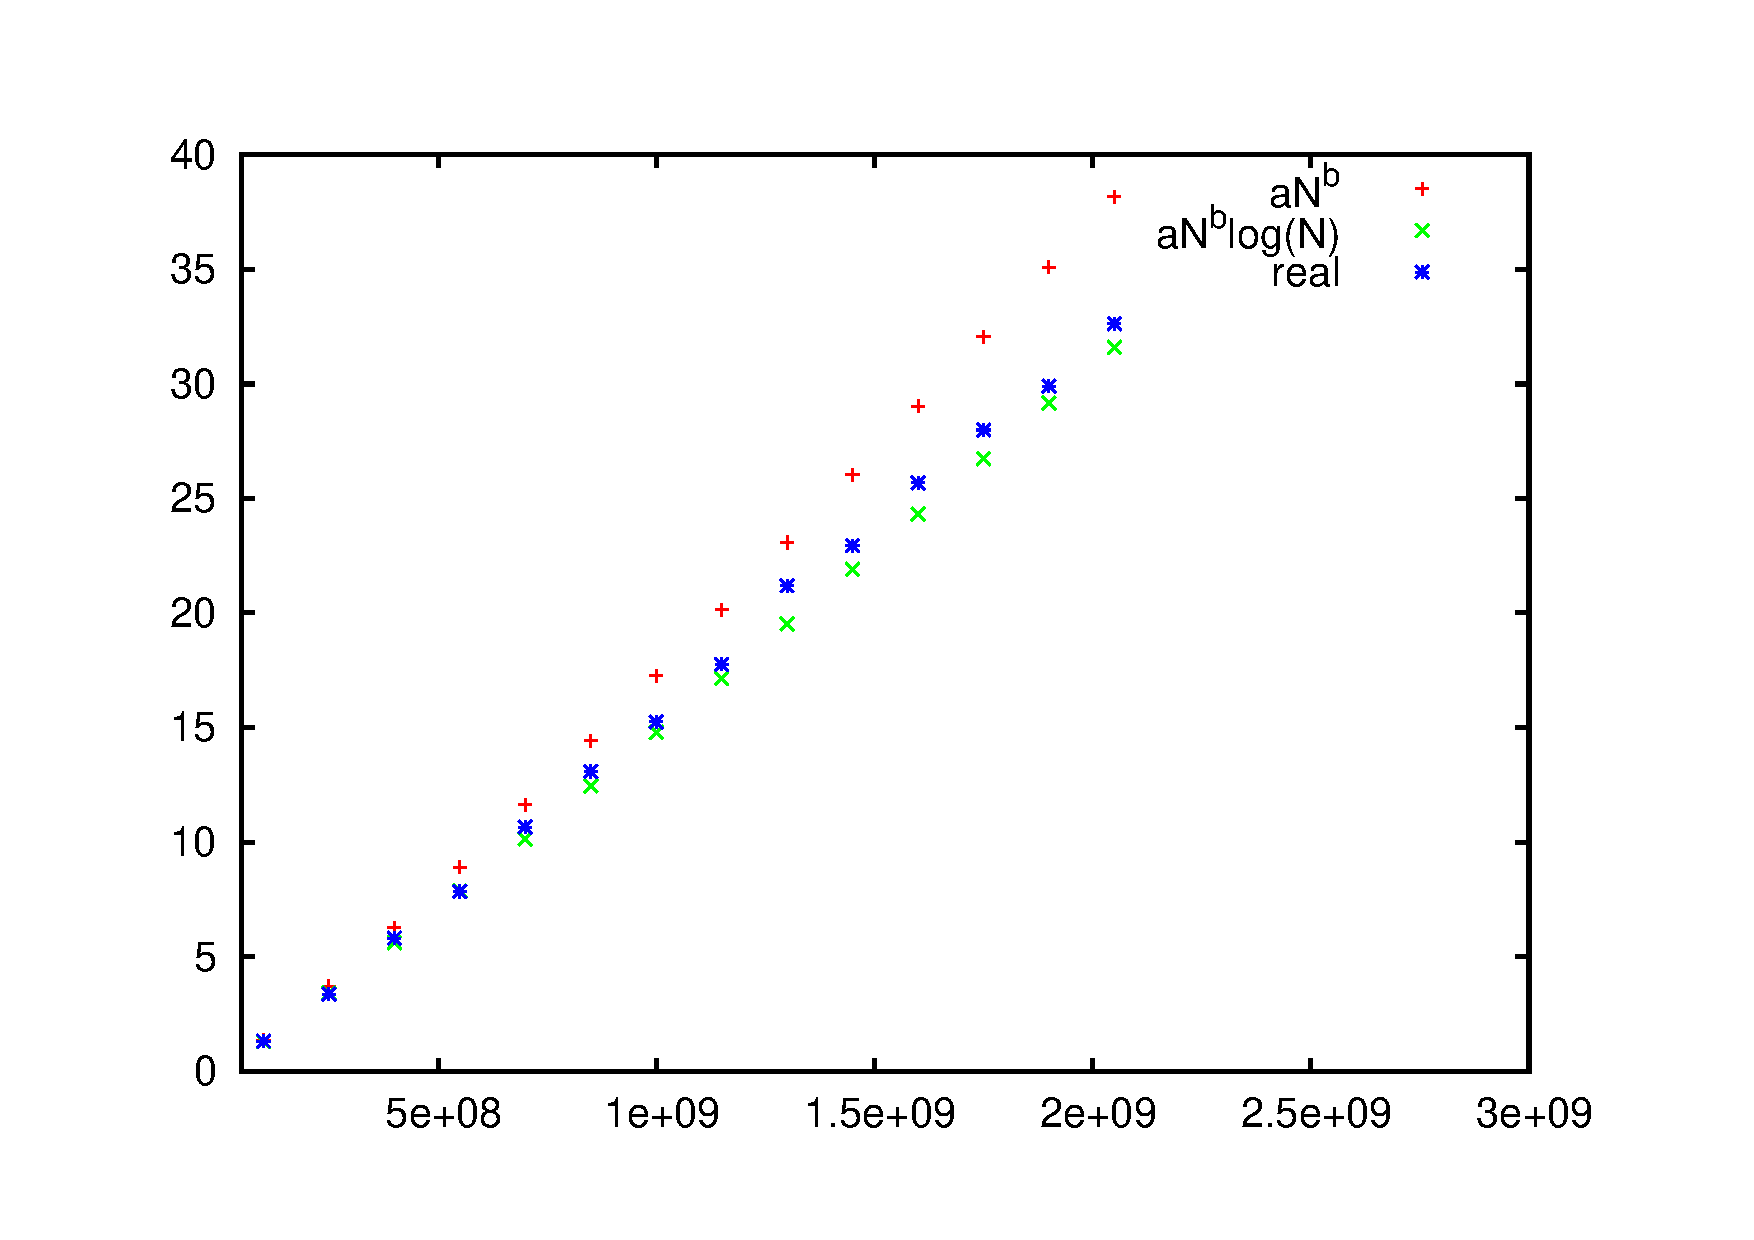
\includegraphics[width=10.5cm]{model.pdf}%
\end{center}

\end{frame}

\subsection{Order of Growth}

\begin{frame}%[containsverbatim]
\frametitle{Order of Growth}

\begin{itemize}
\item The constant \textcolor{blue}{$a$} in the two models \textcolor{blue}{$aN^b$} and \textcolor{blue}{$aN^b\log(N)$}, is dependant on a lot of factors:
\vspace{0.05cm}
\begin{itemize}
\item<1-> Processor, memory, compiler, and so on.
\end{itemize}

\vspace{0.25cm}

\item<2-> The order of growth does not take into account the constant \textcolor{blue}{$a$}.
\vspace{0.05cm}
\begin{itemize}
\item<2-> For example, the order of growth of $T(N) = 12N\log(N)$ is $N\log(N)$.
\end{itemize}

\vspace{0.25cm}

\item<3-> The order of growth allows our complexity analysis to be independant of the machine
on which we run our program.

\end{itemize}

\end{frame}

\begin{frame}%[containsverbatim]
\frametitle{Asymptotic Upper Bound}

\scriptsize

Let $g(n)$ be a positive function. We note $O(g(n))$ the following set:

\begin{block}{Asymptotic Upper Bound}
\begin{tabular}{lcl}
$O(g(n))$ & $=$ &  $\{ f(n)$ : there exist positive constants $c \in \mathbb{R}^+$ and $n_0 \in \mathbb{N}$ such\\
& & \ \ that $0 \le f(n) \le cg(n)$ for all $n \ge n_0 \}$\\
\end{tabular}
\end{block}

\onslide<2->
We use $O$ to give an upper bound on a function within a constant factor and we
note $f(n) = O(g(n))$ instead of $f(n) \in O(g(n))$.\\
\vspace{0.3cm}
\onslide<3->
For example,
\begin{itemize}
\item $23n^2 + 100n + 512 = O(n^2)$.
\item $23n^2 + 100n + 512 = O(n^4)$.
\item $0.5n = O(n)$.
\end{itemize}

\vspace{0.3cm}
\onslide<4->
Intuitively, $f = O(g)$ approximately means that $f \le g$.

\end{frame}

\begin{frame}[containsverbatim]
\frametitle{Asymptotic Upper Bound: Graphical Representation}

\begin{center}
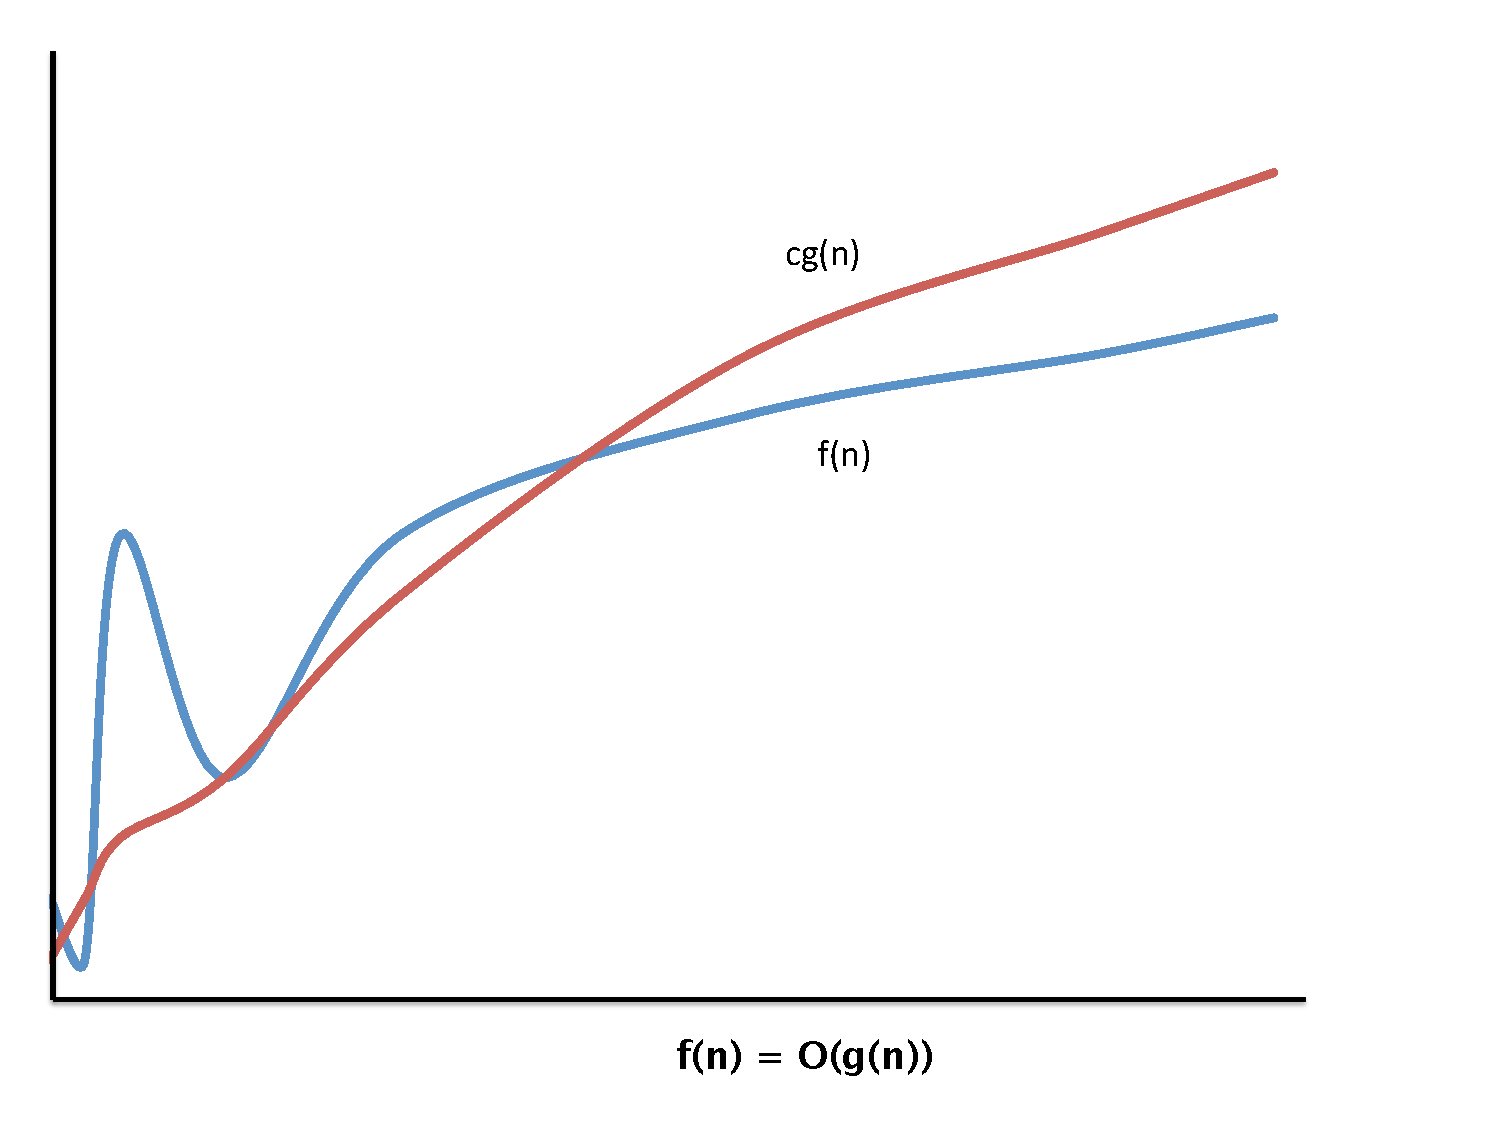
\includegraphics[width=9cm]{big_O.pdf}%
\end{center}

\end{frame}

\begin{frame}%[containsverbatim]
\frametitle{Asymptotic Lower Bound}

\scriptsize

Let $g(n)$ be a positive function. We note $\Omega(g(n))$ the following set:

\begin{block}{Asymptotic Lower Bound}
\begin{tabular}{lcl}
$\Omega(g(n))$ & $=$ & $\{ f(n)$ : there exist positive constants $c \in \mathbb{R}^*$ and $n_0 \in \mathbb{N}$ such\\
& & \ \ that $0 \le cg(n) \le f(n)$ for all $n \ge n_0 \}$\\
\end{tabular}
\end{block}
\onslide<2->
We use $\Omega$ to give an upper bound on a function within a constant factor and we
note $f(n) = \Omega(g(n))$ instead of $f(n) \in \Omega(g(n))$.\\
\vspace{0.3cm}
\onslide<3->
For example,
\begin{itemize}
\item $n^2 = \Omega(0.5n^2)$.
\item $23n^2 + 100n + 512 = \Omega(n^2)$.
\item $n = \Omega(\ln n)$.
\end{itemize}

\vspace{0.3cm}

\onslide<4->
Intuitively, $f = \Omega(g)$ approximately means that $f \ge g$.

\end{frame}

\begin{frame}[containsverbatim]
\frametitle{Asymptotic Lower Bound: Graphical Representation}

\begin{center}
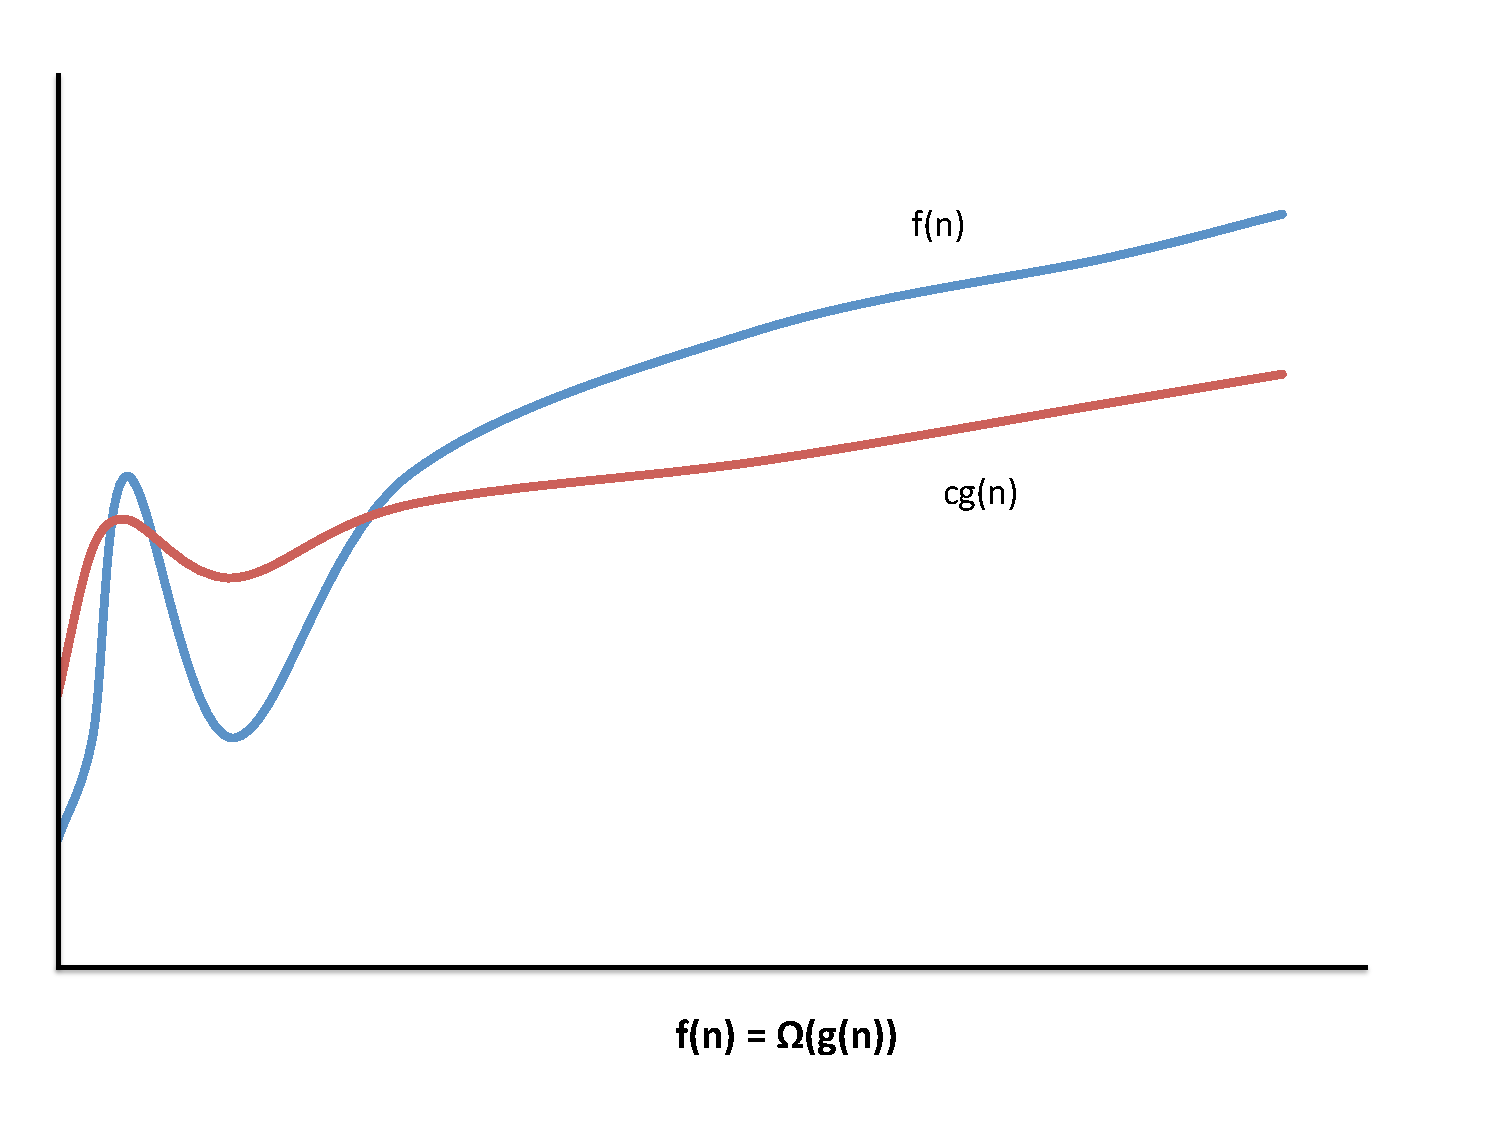
\includegraphics[width=9cm]{big_omega.pdf}%
\end{center}

\end{frame}

\begin{frame}%[containsverbatim]
\frametitle{Asymptotic Tight Bound}

\scriptsize

Let $g(n)$ be a positive function. We note $\Theta(g(n))$ the following set:

\begin{block}{Asymptotic Tight Bound}
\begin{tabular}{lcl}
$\Theta(g(n))$ & $=$ & $\{ f(n)$ : there exist positive constants $c_1 \in \mathbb{R}^*$, $c_2 \in \mathbb{R}^*$ and $n_0 \in \mathbb{N}$\\
& & \ \ such that $0 \le c_1g(n) \le f(n) \le c_2g(n)$ for all $n \ge n_0 \}$\\
\end{tabular}
\end{block}

\onslide<2->
We use $\Theta$ to give a tight bound on a function within a constant factor and we
note $f(n) = \Theta(g(n))$ instead of $f(n) \in \Theta(g(n))$.\\
\vspace{0.3cm}
\onslide<3->
For example,
\begin{itemize}
\item $n^2 = \Theta(0.5n^2)$.
\item $23n^2 + 100n + 512 = \Theta(n^2)$.
\item $n = \Theta(1000n)$.
\end{itemize}

\vspace{0.3cm}
\onslide<4->
Intuitively, $f = \Theta(g)$ approximately means that $f = g$.

\end{frame}

\begin{frame}[containsverbatim]
\frametitle{Asymptotic Tight Bound: Graphical Representation}

\begin{center}
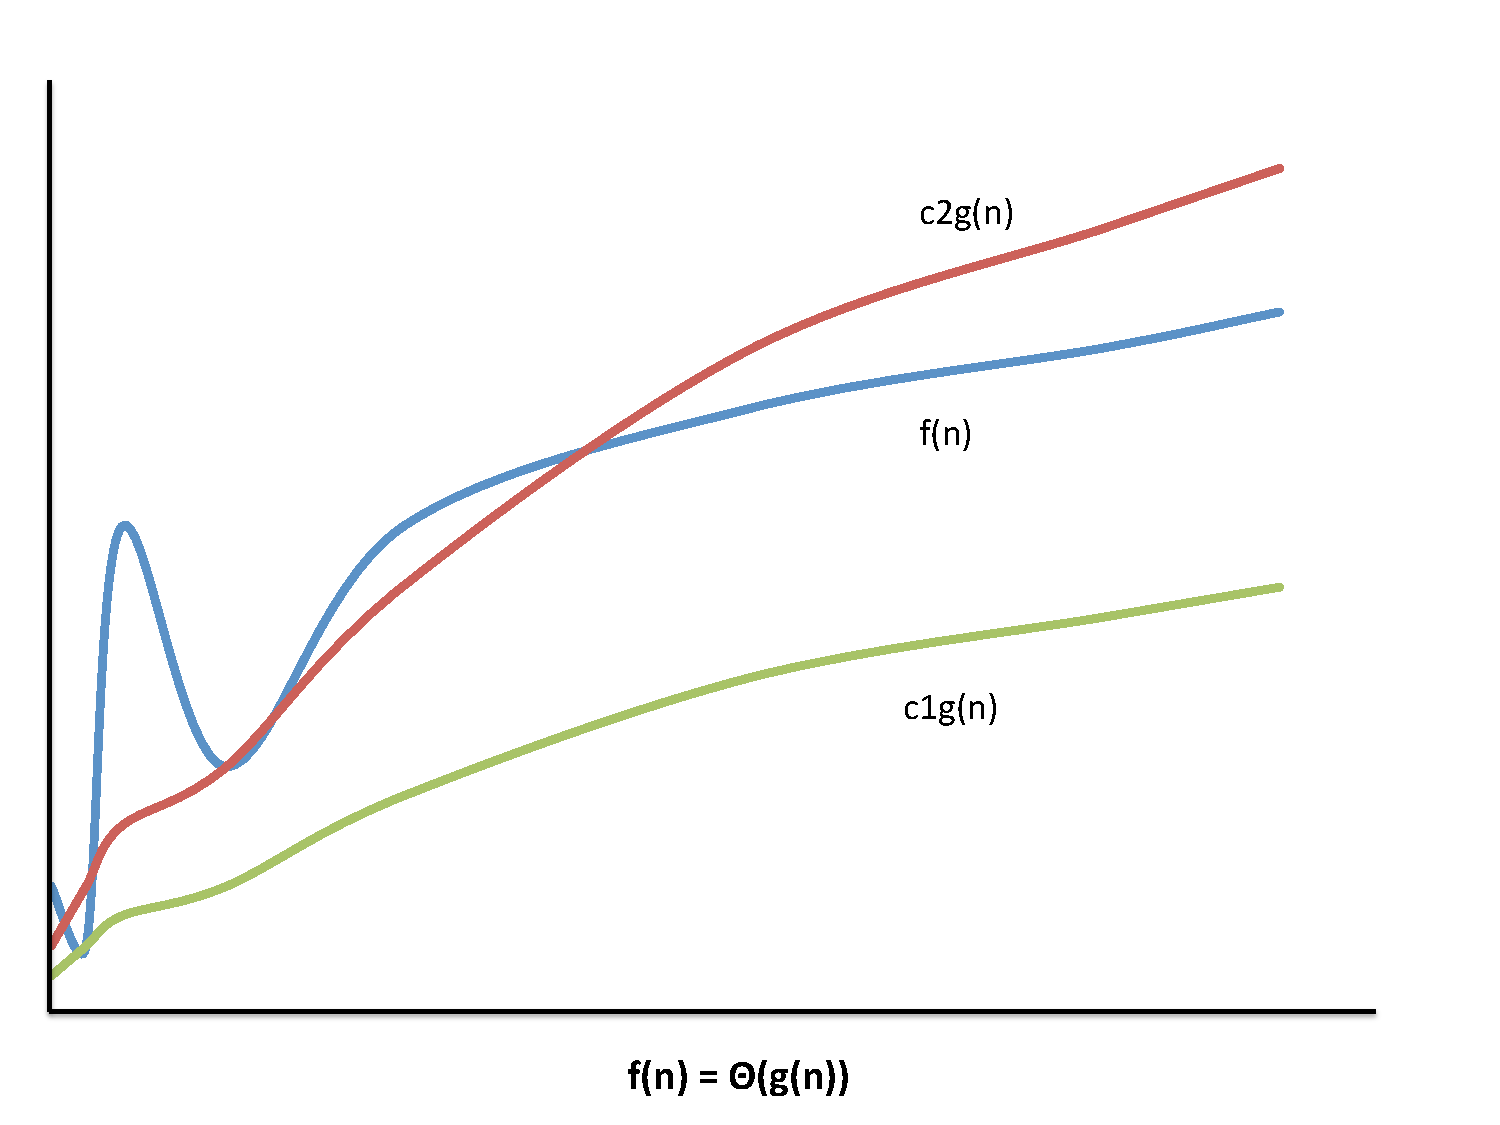
\includegraphics[width=9cm]{big_theta.pdf}%
\end{center}

\end{frame}

\subsection{Logarithmic Complexity}

\begin{frame}%[containsverbatim]
\frametitle{Logarithmic Complexity ($O(\log n)$)}

\begin{itemize}

\item If our algorithm does the following:
\vspace{0.1cm}
\begin{enumerate}

\item<1-> It successively reduce the size of the input by a given factor in each iteration.

\vspace{0.1cm}

\item<2-> In each iteration it does a constant amount of work.

\end{enumerate}

\vspace{0.5cm}

\item<3-> Then, the complexity of our algorithm is logarithmic.

\end{itemize}

\end{frame}

\begin{frame}%[containsverbatim]
\frametitle{Logarithmic Complexity}

\begin{center}
\includegraphics<1>[width=11cm]{logarithmic_complexity1.pdf}%
\includegraphics<2>[width=11cm]{logarithmic_complexity2.pdf}%
\includegraphics<3>[width=11cm]{logarithmic_complexity3.pdf}%
\includegraphics<4>[width=11cm]{logarithmic_complexity4.pdf}%
\includegraphics<5>[width=11cm]{logarithmic_complexity5.pdf}%
%% \includegraphics<6>[width=11cm]{logarithmic_complexity6.pdf}%
%% \includegraphics<7>[width=11cm]{logarithmic_complexity7.pdf}%
%% \includegraphics<8>[width=11cm]{logarithmic_complexity8.pdf}%
\includegraphics<6>[width=11cm]{logarithmic_complexity9.pdf}%
\end{center}

\end{frame}

\begin{frame}%[containsverbatim]
\frametitle{Logarithmic Complexity}

\begin{center}
\includegraphics<1>[width=11cm]{logarithmic_complexity10.pdf}%
\end{center}

\end{frame}

\begin{frame}%[containsverbatim]
\frametitle{Binary Search (Bisection)}

\scriptsize

\begin{mdframed}[style=exampledefault]
Problem: Let
\begin{itemize}
\item $f: ([a,b] \subset \mathbb{R}) \rightarrow \mathbb{R}$ be a monotonic function.
\item $y \in [f(a), f(b)]$.
\item $\epsilon$ an error threshold we can tolerate.
\end{itemize}
Find an $x \in [a,b]$ such that $y \in [f(x - \frac{\epsilon}{2}), f(x + \frac{\epsilon}{2})]$.
\end{mdframed}

\begin{overlayarea}{1\textwidth}{0.7\textheight}
\begin{center}
\includegraphics<2>[width=7cm]{bisection.pdf}%
\includegraphics<3>[width=7cm]{bisection1.pdf}%
\includegraphics<4>[width=7cm]{bisection2.pdf}%
\includegraphics<5>[width=7cm]{bisection2bis.pdf}%
\includegraphics<6>[width=7cm]{bisection3.pdf}%
\includegraphics<7>[width=7cm]{bisection3bis.pdf}%
\includegraphics<8>[width=7cm]{bisection4.pdf}%
\includegraphics<9>[width=7cm]{bisection4bis.pdf}%
\includegraphics<10->[width=7cm]{bisection5.pdf}%
\end{center}
\end{overlayarea}

\end{frame}

\begin{frame}%[containsverbatim]
\frametitle{Binary Search (Bisection)}

\begin{itemize}

\item The number of iterations needed to reach the answer within the given precision is $\lceil\log(\frac{(b - a)}{\epsilon})\rceil$.
\begin{itemize}
\item<1-> Suppose $a = 0$, $b = 1000$ and $\epsilon = 10^{-15}$. We only need
$$
\lceil\log(\frac{1000}{10^{-15}})\rceil = 60 \ \textrm{iterations}.
$$
\end{itemize}

%\vspace{0.2cm}

\item<2-> If the domain of $f$ is $\mathbb{N}$ we get the classical binary search method of a sorted array (see next slide).

\vspace{0.2cm}

\item<3-> We can use the binary search method to solve problems that seems, at first glance,
unrelated to it. We will see two such examples from slide \ref{slide:binary_search_example}.

\end{itemize}

\end{frame}

\begin{frame}%[containsverbatim]
\frametitle{Binary Search Implementation}

\footnotesize

\begin{mdframed}[style=exampledefault]
``I was shocked to learn that the binary search program that Bentley proved correct and subsequently
tested in Chapter 5 of Programming Pearls contains a bug.
Once I tell you what it is, you will understand why it escaped detection for two decades. Lest you think I'm picking on Bentley, let me
tell you how I discovered the bug: The version of binary search that I wrote for the
JDK contained the same bug. It was reported to Sun recently when it broke someone's program, after lying
in wait for nine years or so.'' -- Joshua Bloch (\url{https://research.googleblog.com/2006/06/extra-extra-read-all-about-it-nearly.html})
\end{mdframed}

\end{frame}

\begin{frame}[containsverbatim]
\frametitle{Recursive Implementation}
\scriptsize
\begin{lstlisting}
int binary_search(int key, const vector<int>& v, int lo, int hi)
{
  if (lo > hi) return -1;
  int mid = lo + (hi - lo) / 2;
  if      (key < v[mid]) return binary_search(key, v, lo, mid - 1);
  else if (key > v[mid]) return binary_search(key, v, mid + 1, hi);
  else return mid;
}

int binary_search(int key, const vector<int>& v)
{
  return binary_search(key, v, 0, v.size() - 1);
}
\end{lstlisting}

\end{frame}

\begin{frame}[containsverbatim]
\frametitle{Iterative Implementation}
\scriptsize
A non-recursive version of binary search is given below (the complexity is the same, but faster in practice):

\begin{lstlisting}[mathescape]
int binary_search(int key, const vector<int>& v)
{
  int lo = 0;
  int hi = v.size() - 1;
  while (lo <= hi)
  {
    int mid = lo + (hi - lo) / 2;
    if      (key < v[mid]) hi = mid - 1;
    else if (key > v[mid]) lo = mid + 1;
    else return mid;
  }
  return -1;
}
\end{lstlisting}

\end{frame}

\begin{frame}[containsverbatim]
\frametitle{\exo}

In the preceding \texttt{binary\_search} function, why did we use\\
\vspace{0.2cm}
\begin{lstlisting}[mathescape]
      int mid = lo + (hi - lo) / 2;
\end{lstlisting}
\vspace{0.2cm}
instead of\\
\vspace{0.2cm}
\begin{lstlisting}[mathescape]
      int mid = (lo + hi) / 2;
\end{lstlisting}

\end{frame}

\ifanswers

\begin{frame}[fragile]
\frametitle{Binary Search Bug Solution}

\footnotesize

\setbeamercovered{transparent=0}

Let's initialize \texttt{low} and \texttt{high} with
\begin{lstlisting}[frame=none]
      int lo = 1000000000;
      int hi = 1500000000;
\end{lstlisting}

\onslide<2->

Using

\begin{lstlisting}[frame=none]
      int mid = (lo + hi) / 2;
\end{lstlisting}

we get

\begin{lstlisting}[frame=none]
      mid == -897483648
\end{lstlisting}

\onslide<3->

But using

\begin{lstlisting}[frame=none]
      int mid = lo + (hi - lo) / 2;
\end{lstlisting}

we get

\begin{lstlisting}[frame=none]
      mid == 1250000000
\end{lstlisting}

\end{frame}

\fi

% TopCoder SRM 699 Last Digit
% Codeforces Exams


\begin{frame}%[containsverbatim]
\frametitle{Binary Search Example}
\label{slide:binary_search_example}

\uvalink{12390}{https://uva.onlinejudge.org/index.php?option=onlinejudge&page=show_problem&problem=3812}

\end{frame}

% UVa 12032

\ifanswers

\begin{frame}%[containsverbatim]
\frametitle{12390 Solution}

\begin{itemize}

\item We use the \textbf{work backward} strategy to solve this problem.

\vspace{0.2cm}

\item<2-> We choose a ballot size (maximum number of voters per ballot) and see if everybody
can vote with this ballot size.

\vspace{0.2cm}

\item<3-> To find the best ballot size quickly, we use binary search.

\vspace{0.2cm}

\item<4-> We can use binary search because
\vspace{0.08cm}
\begin{itemize}
\item<4-> If a ballot of size $S$ does not work, all ballots of size $< S$ cannot work either.
\vspace{0.08cm}
\item<5-> We can do a binary search on the interval
$$
[1, \textrm{max\_nb\_inhabitants}],
$$
where \textrm{max\_nb\_inhabitants} is the maximum size of the cities.
\end{itemize}

\end{itemize}

\end{frame}

\begin{frame}[containsverbatim]
\frametitle{12390 Solution}
\scriptsize

\begin{lstlisting}[mathescape]
int main(int argc, char *argv[]) {
  int N, B;
  while (cin >> N >> B && (N != -1 || B != -1))
  {
    vector<int> nb_inhabitants(N, 0);
    int max_nb_inhabitants = 0;
    for (int i = 0; i < N; ++i) {
      cin >> nb_inhabitants[i];
      max_nb_inhabitants = max(max_nb_inhabitants, nb_inhabitants[i]);
    }
    int lo = 1;
    int hi = max_nb_inhabitants;
    while (lo < hi) {
      int mid = lo + (hi - lo) / 2;
      if (possible(B, nb_inhabitants, mid)) hi = mid;
      else lo = mid + 1;
    }
    cout << lo << endl;
  }
}
\end{lstlisting}

\end{frame}

\begin{frame}[containsverbatim]
\frametitle{12390 Solution Implementation}
\scriptsize

\begin{lstlisting}[mathescape]
bool possible(int nb_ballots, const vector<int>& nb_inhabitants,
              int per_ballot)
{
  int remaining_ballots = nb_ballots;
  for (unsigned int i = 0; i < nb_inhabitants.size(); ++i)
  {
    if (nb_inhabitants[i] % per_ballot != 0) --remaining_ballots;
    remaining_ballots -= nb_inhabitants[i] / per_ballot;
    if (remaining_ballots < 0) return false;
  }
  return true;
}
\end{lstlisting}

\end{frame}

\fi

\begin{frame}%[containsverbatim]
\frametitle{\exo}

\codeforceslink{Exams}{http://codeforces.com/contest/732/problem/D}

\end{frame}

\ifanswers

\begin{frame}%[containsverbatim]
\frametitle{Exams Solution}

TO DO

\end{frame}

\begin{frame}[containsverbatim]
\frametitle{Exams Solution Implementation}
\scriptsize

\begin{lstlisting}[mathescape]
const int MAX_SIZE = 100010;
int exams[MAX_SIZE], preparations[MAX_SIZE], positions[MAX_SIZE];
bool possible(int nb_days);

int main(int argc, char *argv[]) {
  int n, m;
  cin >> n >> m;
  for (int i = 0; i < n; ++i) cin >> exams[i];
  for (int i = 1; i <= m; ++i) cin >> preparations[i];
  int lo = 1, hi = n;
  while (lo < hi)
  {
    int mid = lo + (hi - lo) / 2;
    if (possible(mid)) hi = mid;
    else lo = mid + 1;
  }
  if (possible(lo)) cout << lo << endl;
  else cout << -1 << endl;
  return 0;
}
\end{lstlisting}

\end{frame}

\begin{frame}[containsverbatim]
\frametitle{Exams Solution Implementation}
\scriptsize

\begin{lstlisting}[mathescape]
bool possible(int nb_days) {
  for (int i = 0; i < nb_days; ++i)
  {
    positions[exams[i]] = i;
  }
  positions[0] = -1;
  int prep = 0;
  int nb_exams = 0;
  for (int i = 0; i < nb_days; ++i)
  {
    if (positions[exams[i]] == i)
    {
      ++nb_exams;
      if (prep < preparations[exams[i]]) return false;
      prep -= preparations[exams[i]];
    }
    else ++prep;
  }
  return nb_exams == m;
}
\end{lstlisting}

\end{frame}


\fi


\begin{frame}%[containsverbatim]
\frametitle{\exo}

\spojlink{Glasnici}{http://www.spoj.com/problems/GLASNICI/}

\end{frame}

\ifanswers

\begin{frame}%[containsverbatim]
\frametitle{Glasnici Solution}

\scriptsize

\begin{itemize}

\item We use the same methodology than the one used for the last problem, but this time, on real numbers.

\vspace{0.15cm}

\item<2-> We do a binary search on the interval $[0, \textrm{max\_distance}]$ to find the best time.
\begin{itemize}
\scriptsize
\vspace{0.07cm}
\item<2-> \textrm{max\_distance} is the maximum distance from the first village.
\end{itemize}

\vspace{0.15cm}

\item<3-> We can do a binary search, because if a given time \texttt{t} is too short for all messengers
to learn the news, any time \texttt{t'} $<$ \texttt{t} is also too short.

\vspace{0.15cm}

\item<4-> Beware when manipulating floating point numbers, it can be pretty tricky.
\begin{itemize}
\scriptsize
\vspace{0.07cm}
\item<4-> For example,
\begin{itemize}
\scriptsize
\item<4-> \texttt{3.14 + (1e42 - 1e42) = 3.14}, but \texttt{(3.14 + 1e42) - 1e42 = 0}.
\item<5-> \texttt{(1 + (1 + 1e-11)) / 2 = 1 + 5e-12}, but \\\texttt{(1000 + (1000 + 1e-11)) / 2 = 1000 + 1e-11}.
\end{itemize}
\vspace{0.08cm}
\item<6-> To avoid testing the length of the interval for terminating the loop, we reduce
the interval for a fixed number of iterations.
\vspace{0.08cm}
\item<7-> For example, if we halve $100$ times the interval, we get a precision of $\frac{1}{2^{100}}$ (or the maximum
precision we can get with \lstinline{float} or \lstinline{double}).

\end{itemize}

\end{itemize}

\end{frame}

\begin{frame}%[containsverbatim]
\frametitle{Glasnici Solution}

\begin{center}
\includegraphics<1>[width=12cm]{glasnici.pdf}%
\includegraphics<2>[width=12cm]{glasnici1.pdf}%
\includegraphics<3>[width=12cm]{glasnici2.pdf}%
\includegraphics<4>[width=12cm]{glasnici3.pdf}%
\includegraphics<5>[width=12cm]{glasnici4.pdf}%
\includegraphics<6>[width=12cm]{glasnici5.pdf}%
\includegraphics<7>[width=12cm]{glasnici6.pdf}%
\includegraphics<8>[width=12cm]{glasnici7.pdf}%
\includegraphics<9>[width=12cm]{glasnici7_1.pdf}%
\includegraphics<10>[width=12cm]{glasnici7_2.pdf}%
\includegraphics<11>[width=12cm]{glasnici8.pdf}%
\includegraphics<12>[width=12cm]{glasnici9.pdf}%
\end{center}

\end{frame}

\begin{frame}[containsverbatim]
\frametitle{Glasnici Solution Implementation}
\scriptsize

\begin{lstlisting}[mathescape]
int main(int argc, char *argv[]) {
  int tc; cin >> tc;
  while (tc--)
  {
    double K;
    int N; cin >> K >> N;
    vector<double> distances(N, 0);
    for (int i = 0; i < N; ++i) cin >> distances[i];
    double lo = 0;
    double hi = distances[N - 1];
    double mid;
    for (int i = 0; i < 100; ++i) {
      mid = lo + (hi - lo) / 2;
      if (possible(K, mid, distances)) hi = mid;
      else lo = mid;
    }
    cout << fixed << setprecision(2) << mid << endl;
    // printf("%.2lf\n", mid);
  }
}
\end{lstlisting}

\end{frame}

\begin{frame}[containsverbatim]
\frametitle{Glasnici Solution Implementation}
\scriptsize

\begin{lstlisting}[mathescape]
bool possible(double K, double time,
              const vector<double>& distances)
{
  double current_position = distances[0] + time;
  for (unsigned int i = 1; i < distances.size(); ++i)
  {
    if (current_position + K < distances[i] - time) return false;
    current_position = min(current_position + K, distances[i] + time);
  }
  return true;
}
\end{lstlisting}

\end{frame}

\fi


\begin{frame}%[containsverbatim]
\frametitle{\exo}

\codeforceslink{Road to Cinema}{http://codeforces.com/contest/729/problem/C}

\end{frame}

\ifanswers

\begin{frame}%[containsverbatim]
\frametitle{Road to Cinema Solution}

TO DO

\end{frame}

\begin{frame}[containsverbatim]
\frametitle{Road to Cinema Solution Implementation}
\scriptsize

\begin{lstlisting}[mathescape]
vector<int> stations;
int nb_stations, starting_time;

bool possible(int capacity)
{
  long long time = 0;
  for (int i = 1; i <= nb_stations + 1; ++i)
  {
    int d = stations[i] - stations[i - 1];
    int full_speed = min(capacity - d, d);
    if (full_speed < 0) return false;
    int min_speed = d - full_speed;
    time += full_speed + 2 * min_speed;
    if (time > starting_time) return false;
  }
  return true;
}
\end{lstlisting}

\end{frame}

\begin{frame}[containsverbatim]
\frametitle{Road to Cinema Solution Implementation}
\scriptsize

\begin{lstlisting}[mathescape]
int main(int argc, char *argv[]) {
  int N, road_length;
  ios::sync_with_stdio(false);
  cin >> N >> nb_stations >> road_length >> starting_time;
  vector<pair<int, int>> cars(N);
  for (int i = 0; i < N; ++i)
    cin >> cars[i].first >> cars[i].second;
  stations.assign(nb_stations + 2, 0);
  for (int i = 1; i <= nb_stations; ++i)
    cin >> stations[i];
  stations[nb_stations + 1] = road_length;
  sort(stations.begin(), stations.end());

  int lo = 0, hi = starting_time;
  while (lo < hi) {
    int mid = lo + (hi - lo) / 2;
    if (possible(mid)) hi = mid;
    else lo = mid + 1;
  }
  // ...
\end{lstlisting}

\end{frame}

\begin{frame}[containsverbatim]
\frametitle{Road to Cinema Solution Implementation}
\scriptsize

\begin{lstlisting}[mathescape]
  // ...
  int price = 2e9;
  if (possible(lo))
    {
      for (int i = 0; i < N; ++i)
        {
          if (cars[i].second >= lo) price = min(price, cars[i].first);
        }
    }
  if (price == 2e9) cout << -1 << endl;
  else cout << price << endl;
  return 0;
}
\end{lstlisting}

\end{frame}

\fi

\begin{frame}%[containsverbatim]
\frametitle{\exo}

TO DO
%\kattislink{}{}

%cutting cheese

\end{frame}

\ifanswers

\begin{frame}%[containsverbatim]
\frametitle{}

TO DO

\end{frame}

\begin{frame}[containsverbatim]
\frametitle{}
\scriptsize

\begin{lstlisting}[mathescape]
\end{lstlisting}

\end{frame}

\begin{frame}[containsverbatim]
\frametitle{}
\scriptsize

\begin{lstlisting}[mathescape]
\end{lstlisting}

\end{frame}

\begin{frame}[containsverbatim]
\frametitle{}
\scriptsize

\begin{lstlisting}[mathescape]
\end{lstlisting}

\end{frame}

\fi

\begin{frame}%[containsverbatim]
\frametitle{\exo}

\codeforceslink{New Year and Rating}{http://codeforces.com/contest/750/problem/C}

\end{frame}

\ifanswers

\begin{frame}%[containsverbatim]
\frametitle{New Year and Rating Solution}

TO DO

\end{frame}

\begin{frame}[containsverbatim]
\frametitle{New Year and Rating Solution Implementation}
\scriptsize

\begin{lstlisting}[mathescape]
\end{lstlisting}

\end{frame}

\begin{frame}[containsverbatim]
\frametitle{New Year and Rating Solution Implementation}
\scriptsize

\begin{lstlisting}[mathescape]
\end{lstlisting}

\end{frame}

\begin{frame}[containsverbatim]
\frametitle{New Year and Rating Solution Implementation}
\scriptsize

\begin{lstlisting}[mathescape]
\end{lstlisting}

\end{frame}

\fi

% BRII SPOJ

\begin{frame}%[containsverbatim]
\frametitle{Ternary Search}

\setbeamercovered{transparent=0}

\footnotesize

\begin{block}{Definition}
A function $f$ is \textbf{unimodal} on $[a, b]$ if it is
\begin{itemize}
\item[a)] Strictly increasing.
\item[b)] Strictly decreasing.
\item[c)] Strictly increasing and then strictly decreasing.
%\item[d)] Strictly decreasing and then strictly increasing.
\end{itemize}
\end{block}

\begin{overlayarea}{1\textwidth}{0.5\textheight}
\begin{center}
\includegraphics<2>[width=5cm]{unimodal2.pdf}%
\includegraphics<3>[width=5cm]{unimodal3.pdf}%
\includegraphics<4>[width=5cm]{unimodal.pdf}%
%\includegraphics<5->[width=5cm]{unimodal1.pdf}%
\end{center}
\end{overlayarea}

\end{frame}

\begin{frame}%[containsverbatim]
\frametitle{Ternary Search}

\setbeamercovered{transparent=0}

\footnotesize

\begin{mdframed}[style=exampledefault]
Problem: Let
\begin{itemize}
\item $f: ([a,b] \subset \mathbb{R}) \rightarrow \mathbb{R}$ be a unimodal function of type a), b) or c).
\item $f^* = \max_{x \in [a,b]} f(x)$.
\item $\epsilon$ an error threshold we can tolerate.
\end{itemize}
Find an $x \in [a,b]$ such that
$f^* \in [f(x - \frac{\epsilon}{2}), f(x + \frac{\epsilon}{2})]$.
\end{mdframed}

\begin{overlayarea}{1\textwidth}{0.6\textheight}
\begin{center}
\includegraphics<2>[width=6cm]{ternary_search.pdf}%
\includegraphics<3>[width=6cm]{ternary_search1.pdf}%
\includegraphics<4>[width=6cm]{ternary_search2.pdf}%
\includegraphics<5>[width=6cm]{ternary_search3.pdf}%
\includegraphics<6>[width=6cm]{ternary_search4.pdf}%
\includegraphics<7>[width=6cm]{ternary_search5.pdf}%
\includegraphics<8>[width=6cm]{ternary_search6.pdf}%
\end{center}
\end{overlayarea}

\end{frame}

\begin{frame}[containsverbatim]
\frametitle{Discrete Ternary Search Iterative Implementation}
\scriptsize

\begin{lstlisting}[mathescape]
// v is unimodal of type a), b) or c) or v is constant
int ternary_search(const vector<int>& v)
{
  int lo = 0;
  int hi = v.size() - 1;
  while (lo < hi)
  {
    int left_third = lo + (hi - lo) / 3;
    int right_third = hi - (hi - lo) / 3;
    if (v[left_third] < v[right_third]) lo = left_third + 1;
    else hi = right_third - 1;
  }
  return lo;
}
\end{lstlisting}

\end{frame}

\begin{frame}%[containsverbatim]
\frametitle{Ternary Search Example}

\lightojlink{1146}{http://www.lightoj.com/volume_showproblem.php?problem=1146}

\end{frame}

\ifanswers

\begin{frame}%[containsverbatim]
\frametitle{1146 Solution}

\scriptsize

\setbeamercovered{transparent=0}

\begin{itemize}

\item The distance between the two men is constant or a unimodal function of type a), b) or d).

\begin{overlayarea}{1\textwidth}{0.45\textheight}
\begin{center}
\includegraphics<2>[width=4.5cm]{closest_distance.pdf}%
\includegraphics<3>[width=4.5cm]{closest_distance1.pdf}%
\includegraphics<4>[width=4.5cm]{closest_distance2.pdf}%
\includegraphics<5>[width=4.5cm]{closest_distance3.pdf}%
\includegraphics<6>[width=4.5cm]{closest_distance4.pdf}%
\includegraphics<7>[width=4.5cm]{closest_distance5.pdf}%
\includegraphics<8>[width=4.5cm]{closest_distance6.pdf}%
\includegraphics<9>[width=4.5cm]{closest_distance9.pdf}%
\includegraphics<10>[width=4.5cm]{closest_distance10.pdf}%
\includegraphics<11>[width=4.5cm]{closest_distance11.pdf}%
\includegraphics<12>[width=4.5cm]{closest_distance12.pdf}%
\includegraphics<13>[width=4.5cm]{closest_distance13.pdf}%
\includegraphics<14>[width=4.5cm]{closest_distance14.pdf}%
\includegraphics<15>[width=4.5cm]{closest_distance15.pdf}%
\includegraphics<16>[width=4.5cm]{closest_distance7.pdf}%
\includegraphics<17>[width=4.5cm]{closest_distance16.pdf}%
\includegraphics<18->[width=4.5cm]{closest_distance8.pdf}%
\end{center}
\end{overlayarea}

%\vspace{0.2cm}

\item<19-> Because the two men maintain constant velocities and reach their destinations
at the same time, we can use ternary search on the segment $[0,1]$.
\begin{itemize}
\scriptsize
%\vspace{0.2cm}
\vspace{0.08cm}
\item<20-> An element of $r \in [0, 1]$ represents the ratio of the distance covered to the total distance.
\vspace{0.1cm}
\item<21-> The first man is located at $(A_x + r \times (B_x - A_x), A_y + r \times (B_y - A_y))$.
\vspace{0.1cm}
\item<22-> The second man is located at $(C_x + r \times (D_x - C_x), C_y + r \times (D_y - C_y))$.

\end{itemize}

\end{itemize}

\end{frame}

\begin{frame}[containsverbatim]
\frametitle{1146 Solution Implementation}
\scriptsize

\begin{lstlisting}[mathescape]
int ax, ay, bx, by, cx, cy, dx, dy;

double distance(double ratio)
{
  double first_man_x = ax + ratio * (bx - ax);
  double first_man_y = ay + ratio * (by - ay);
  double second_man_x = cx + ratio * (dx - cx);
  double second_man_y = cy + ratio * (dy - cy);
  double delta_x = first_man_x - second_man_x;
  double delta_y = first_man_y - second_man_y;
  return sqrt(delta_x * delta_x + delta_y * delta_y);
}
\end{lstlisting}

\end{frame}

\begin{frame}[containsverbatim]
\frametitle{1146 Solution Implementation}
\scriptsize

\begin{lstlisting}[mathescape]
int main(int argc, char *argv[]) {
  int TC;
  cin >> TC;
  for (int tc = 1; tc <= TC; ++tc)
  {
    cin >> ax >> ay >> bx >> by >> cx >> cy >> dx >> dy;
    double lo = 0;
    double hi = 1;
    for (int i = 0; i < 100; ++i)
    {
      double left_third = lo + (hi - lo) / 3;
      double right_third = hi - (hi - lo) / 3;
      if (distance(left_third)<distance(right_third)) hi = right_third;
      else lo = left_third;
    }
    cout << "Case " << tc << ": " << setprecision(8)
         << distance(lo) << endl;
  }
  return 0;
}
\end{lstlisting}

\end{frame}

\fi

\begin{frame}%[containsverbatim]
\frametitle{\exo}

\uvalink{13010}{https://uva.onlinejudge.org/index.php?option=com_onlinejudge&Itemid=8&category=24&page=show_problem&problem=4898}
\vspace{0.4cm}
\hint{
Have a look at \hyperlink{slide:dijkstra_algorithm}{Dijkstra's algorithm} in the \hyperlink{slide:graphs}{Graphs part} of this volume.
}

\end{frame}

\ifanswers

\begin{frame}%[containsverbatim]
\frametitle{13010 Solution}

\footnotesize

\begin{itemize}

\item<1-> The minimum cost between the source \emph{ACM} office (office $1$) and the destination
\emph{ACM} office (office $N$) is a function of the time $t$, let's call it \textcolor{blue}{\texttt{min\_cost}}.

\vspace{0.15cm}

\item<2-> If the \textcolor{blue}{\texttt{min\_cost}} function is constant or a unimodal function of type a), b) or c), we can apply
ternary search on the interval $[0, 24\times60]$ to find the maximum cost.

\vspace{0.15cm}

\item<3-> Let's see now why \textcolor{blue}{\texttt{min\_cost}} is constant or a unimodal function of type a), b) or c).
\begin{itemize}
\footnotesize
\item<3-> The cost of each possible paths between office $1$ and office $N$ is a linear function of $t$. Indeed, the sum
of some linear functions is a linear function:
$$
(A_1\times t + B_1) + (A_2\times t + B_2) = (A_1 + A_2) \times t + (B_1 + B_2).
$$
\item<4-> The minimum of a set of linear functions on $[a,b]$ is constant or a unimodal function of type a), b) or c) on $[a,b]$ with one exception:
The resulting function can have a plateau at its maximum, but ternary search still works in this case.

\end{itemize}

\end{itemize}

\end{frame}

\begin{frame}%[containsverbatim]
\frametitle{13010 Solution}

\begin{center}
\includegraphics<1>[width=9cm]{min_linear.pdf}%
\includegraphics<2>[width=9cm]{min_linear1.pdf}%
\includegraphics<3>[width=9cm]{min_linear2.pdf}%
\includegraphics<4>[width=9cm]{min_linear3.pdf}%
\end{center}

\end{frame}

\begin{frame}[containsverbatim]
\frametitle{13010 Solution Implementation}
\scriptsize

\begin{lstlisting}[mathescape]
int main(int argc, char *argv[])
{
  int N, M;
  while (cin >> N >> M)
  {
    graph g(N + 1);
    for (int i = 0; i < M; ++i)
    {
      int I, J;
      int A, B;
      cin >> I >> J >> A >> B;
      g.add_edge(I, J, {A, B});
    }
    // ...
\end{lstlisting}

\end{frame}

\begin{frame}[containsverbatim]
\frametitle{13010 Solution Implementation}
\scriptsize

\begin{lstlisting}[mathescape]
    // ...
    double lo = 0;
    double hi = 24 * 60;
    for (int i = 0; i < 100; ++i)
    {
      double left_third = lo + (hi - lo) / 3;
      double right_third = hi - (hi - lo) / 3;
      dijkstra dj_lo(g, 1, left_third);
      dijkstra dj_hi(g, 1, right_third);
      if (dj_lo.total_tax(N) < dj_hi.total_tax(N)) lo = left_third;
      else hi = right_third;
    }
    cout << fixed << setprecision(5)
         << dijkstra(g, 1, lo).total_tax(N) << endl;
  }
  return 0;
}
\end{lstlisting}

\end{frame}

\begin{frame}[containsverbatim]
\frametitle{13010 Solution Implementation}
\scriptsize

\begin{lstlisting}[mathescape]
struct tax {
  int A;
  int B;
};

class graph {
public:
  typedef vector<pair<int, tax>> NEIGHBORS;
  typedef vector<NEIGHBORS> ADJ_LIST;
  // ...
public:
  // ...
  void add_edge(int i, int j, const tax& t)
  {
    nb_edges++;
    adj[i].push_back(make_pair(j, t));
    if (!directed) adj[j].push_back(make_pair(i, t));
  }
  // ...
\end{lstlisting}

\end{frame}

\begin{frame}[containsverbatim]
\frametitle{13010 Solution Implementation}
\scriptsize

\begin{lstlisting}[mathescape]
class dijkstra {
  const double INF = numeric_limits<double>::max();
  struct node
  {
    double taxes;
    int vertex;
    node(double taxes, int v) : taxes(taxes), vertex(v) {}
    bool operator<(const node& n) const
    {
      return taxes > n.taxes;
    }
  };
  vector<double> dist;
  vector<bool> visited;
public:
  double total_tax(int v) const
  {
    return dist[v];
  }
  // ...
\end{lstlisting}

\end{frame}

\begin{frame}[containsverbatim]
\frametitle{13010 Solution Implementation}
\scriptsize

\begin{lstlisting}[mathescape]
  dijkstra(const graph& g, int s, double t):dist(g.number_of_vertices(),INF), visited(g.number_of_vertices(), false)
  {
    priority_queue<node> pq; pq.push(node(0, s)); dist[s] = 0;
    while (!pq.empty())
    {
      node front = pq.top(); pq.pop();
      if (visited[front.vertex]) continue;
      visited[front.vertex] = true;
      for (const auto& neighbor : g.neighbors(front.vertex))
      {
        double cost = front.taxes + neighbor.second.A * t
                                  + neighbor.second.B;
        if (cost < dist[neighbor.first]) {
          dist[neighbor.first] = cost;
          pq.push(node(cost, neighbor.first));
        }
      }
    }
  }};
\end{lstlisting}

\end{frame}

\fi

\subsection{Linearithmetic Complexity}

\begin{frame}%[containsverbatim]
\frametitle{Linearithmetic Complexity ($O(n \log n)$)}

\begin{itemize}

\item This is the complexity of the best sorting by comparison algorithms.

\vspace{0.4cm}

\item<2-> If your algorithm do the following, it will give rise to a linearithmetic complexity:
\vspace{0.2cm}
\begin{itemize}
\item<3-> Divides the problem size $n$ into $k$ subproblems of size $\frac{n}{k}$ in \textbf{linear time}.
\vspace{0.2cm}
\item<4-> Solves the $k$ subproblems recursively.
\vspace{0.2cm}
\item<5-> Combines the $k$ solutions into overall solution in \textbf{linear time}.
\end{itemize}

\end{itemize}

\end{frame}

\begin{frame}%[containsverbatim]
\frametitle{Linearithmetic vs Linear Complexity}

%\begin{overlayarea}{1\textwidth}{1\textheight}
\begin{center}
\includegraphics<1>[width=10cm]{nlogn_vs_n.pdf}%
\includegraphics<2>[width=10cm]{nlogn_vs_n_1.pdf}%
\includegraphics<3>[width=10cm]{nlogn_vs_n_2.pdf}%
\end{center}
%\end{overlayarea}

\end{frame}

\begin{frame}%[containsverbatim]
\frametitle{Linearithmetic vs Quadratic Complexity}

%\begin{overlayarea}{1\textwidth}{1\textheight}
\begin{center}
\includegraphics<1>[width=10cm]{nlogn_vs_nn.pdf}%
\includegraphics<2>[width=10cm]{nlogn_vs_nn_1.pdf}%
\includegraphics<3>[width=10cm]{nlogn_vs_nn_2.pdf}%
\end{center}
%\end{overlayarea}

\end{frame}

\begin{frame}%[containsverbatim]
\frametitle{Linearithmetic vs Linear vs Quadratic Complexity}

%\begin{overlayarea}{1\textwidth}{1\textheight}
\begin{center}
\includegraphics<1>[width=10cm]{nlogn_vs_n_vs_nn.pdf}%
\includegraphics<2>[width=10cm]{nlogn_vs_n_vs_nn_1.pdf}%
\includegraphics<3>[width=10cm]{nlogn_vs_n_vs_nn_2.pdf}%
\end{center}
%\end{overlayarea}

\end{frame}

\begin{frame}%[containsverbatim]
\frametitle{Merge Sort}

\setbeamercovered{transparent=0}

\begin{mdframed}[style=exampledefault]
Problem: Given an array of $n$ elements, where each elements can be compared, rearrange the elements in ascending order.
\end{mdframed}

\vspace{0.5cm}

\begin{itemize}

\item<2-> One possible solution to this problem consists of the following three steps:
\vspace{0.3cm}
\begin{enumerate}
\item<2-> Recursively sort left half part of the array.

\vspace{0.4cm}

\item<3-> Recursively sort right half part of the array.

\vspace{0.4cm}

\item<4-> Merge the two halves to make the whole array sorted.

\end{enumerate}

\end{itemize}

\end{frame}

\begin{frame}%[containsverbatim]
\frametitle{Merge Sort}

\begin{center}
\includegraphics<1>[width=12cm]{merge_sort.pdf}%
\includegraphics<2>[width=12cm]{merge_sort1.pdf}%
\includegraphics<3>[width=12cm]{merge_sort2.pdf}%
\includegraphics<4>[width=12cm]{merge_sort3.pdf}%
\includegraphics<5>[width=12cm]{merge_sort4.pdf}%
\includegraphics<6>[width=12cm]{merge_sort5.pdf}%
\includegraphics<7>[width=12cm]{merge_sort6.pdf}%
\includegraphics<8>[width=12cm]{merge_sort7.pdf}%
\includegraphics<9>[width=12cm]{merge_sort8.pdf}%
\includegraphics<10>[width=12cm]{merge_sort9.pdf}%
\includegraphics<11>[width=12cm]{merge_sort10.pdf}%
\includegraphics<12>[width=12cm]{merge_sort11.pdf}%
\includegraphics<13>[width=12cm]{merge_sort12.pdf}%
\includegraphics<14>[width=12cm]{merge_sort13.pdf}%
\includegraphics<15>[width=12cm]{merge_sort14.pdf}%
\includegraphics<16>[width=12cm]{merge_sort15.pdf}%
\includegraphics<17>[width=12cm]{merge_sort16.pdf}%
\includegraphics<18>[width=12cm]{merge_sort17.pdf}%
\includegraphics<19>[width=12cm]{merge_sort18.pdf}%
\includegraphics<20>[width=12cm]{merge_sort19.pdf}%
\includegraphics<21>[width=12cm]{merge_sort20bis.pdf}%
\includegraphics<22>[width=12cm]{merge_sort20.pdf}%
\includegraphics<23>[width=12cm]{merge_sort21.pdf}%
\includegraphics<24>[width=12cm]{merge_sort22.pdf}%
\includegraphics<25>[width=12cm]{merge_sort23.pdf}%
\includegraphics<26>[width=12cm]{merge_sort24.pdf}%
\includegraphics<27>[width=12cm]{merge_sort25.pdf}%
\includegraphics<28>[width=12cm]{merge_sort26.pdf}%
\includegraphics<29>[width=12cm]{merge_sort27.pdf}%
\includegraphics<30>[width=12cm]{merge_sort28.pdf}%
\includegraphics<31>[width=12cm]{merge_sort29.pdf}%
\includegraphics<32>[width=12cm]{merge_sort30.pdf}%
\includegraphics<33>[width=12cm]{merge_sort31.pdf}%
\includegraphics<34>[width=12cm]{merge_sort32.pdf}%
\includegraphics<35>[width=12cm]{merge_sort33.pdf}%
\includegraphics<36>[width=12cm]{merge_sort34.pdf}%
\includegraphics<37>[width=12cm]{merge_sort35.pdf}%
\includegraphics<38>[width=12cm]{merge_sort36.pdf}%
\includegraphics<39>[width=12cm]{merge_sort37.pdf}%
\includegraphics<40>[width=12cm]{merge_sort38.pdf}%
\includegraphics<41>[width=12cm]{merge_sort39.pdf}%
\includegraphics<42>[width=12cm]{merge_sort40.pdf}%
\includegraphics<43>[width=12cm]{merge_sort41.pdf}%
\includegraphics<44>[width=12cm]{merge_sort42.pdf}%
\includegraphics<45>[width=12cm]{merge_sort43.pdf}%
\includegraphics<46>[width=12cm]{merge_sort44.pdf}%
\includegraphics<47>[width=12cm]{merge_sort45.pdf}%
\includegraphics<48>[width=12cm]{merge_sort46.pdf}%
\includegraphics<49>[width=12cm]{merge_sort47.pdf}%
\includegraphics<50>[width=12cm]{merge_sort48.pdf}%
\includegraphics<51>[width=12cm]{merge_sort49.pdf}%
\includegraphics<52>[width=12cm]{merge_sort50.pdf}%
\includegraphics<53>[width=12cm]{merge_sort51.pdf}%
\includegraphics<54>[width=12cm]{merge_sort52.pdf}%
\includegraphics<55>[width=12cm]{merge_sort53.pdf}%
\includegraphics<56>[width=12cm]{merge_sort54.pdf}%
\includegraphics<57>[width=12cm]{merge_sort55.pdf}%
\includegraphics<58>[width=12cm]{merge_sort56.pdf}%
\includegraphics<59>[width=12cm]{merge_sort57.pdf}%
\includegraphics<60>[width=12cm]{merge_sort58.pdf}%
\includegraphics<61>[width=12cm]{merge_sort59.pdf}%
\includegraphics<62>[width=12cm]{merge_sort60.pdf}%
\includegraphics<63>[width=12cm]{merge_sort61.pdf}%
\includegraphics<64>[width=12cm]{merge_sort62.pdf}%
\includegraphics<65>[width=12cm]{merge_sort63.pdf}%
\includegraphics<66>[width=12cm]{merge_sort64.pdf}%
\includegraphics<67>[width=12cm]{merge_sort65.pdf}%
\includegraphics<68>[width=12cm]{merge_sort66.pdf}%
\includegraphics<69>[width=12cm]{merge_sort67.pdf}%
\end{center}

\end{frame}

\begin{frame}%[containsverbatim]
\frametitle{Merge Sort Analysis}

\begin{center}
\includegraphics<1>[width=12cm]{merge_sort68.pdf}%
\includegraphics<2>[width=12cm]{merge_sort69.pdf}%
\includegraphics<3>[width=12cm]{merge_sort70.pdf}%
\includegraphics<4>[width=12cm]{merge_sort71.pdf}%
\includegraphics<5>[width=12cm]{merge_sort72.pdf}%
\end{center}

\end{frame}

\begin{frame}[containsverbatim]
\frametitle{Merge Sort Implementation}

\scriptsize

\begin{lstlisting}
void sort(vector<int>& v, vector<int>& aux, int lo, int hi)
{
  if (hi <= lo) return;
  int mid = lo + (hi - lo) / 2;
  sort(v, aux, lo, mid);
  sort(v, aux, mid + 1, hi);
  merge(v, aux, lo, mid, hi);
}

void sort(vector<int>& v)
{
  vector<int> aux(v.size(), 0);
  sort(v, aux, 0, v.size() - 1);
}
\end{lstlisting}

\end{frame}

\begin{frame}[containsverbatim]
\frametitle{Merge Sort Implementation}

\scriptsize

\begin{lstlisting}
void merge(vector<int>& v, vector<int>& aux, int lo, int mid, int hi)
{
  for (int k = lo; k <= hi; k++)
  {
    aux[k] = v[k];
  }

  int i = lo, j = mid+1;
  for (int k = lo; k <= hi; k++)
  {
    if      (i > mid)         v[k] = aux[j++];
    else if (j > hi)          v[k] = aux[i++];
    else if (aux[j] < aux[i]) v[k] = aux[j++];
    else                      v[k] = aux[i++];
  }
}
\end{lstlisting}

\end{frame}

\begin{frame}%[containsverbatim]
\frametitle{\exo}

\uvalink{10810}{https://uva.onlinejudge.org/index.php?option=com_onlinejudge&Itemid=8&category=24&page=show_problem&problem=1751}

\vspace{0.3cm}

\hint{Counting swaps is equivalent to counting inversions.

\begin{overlayarea}{1\textwidth}{0.5\textheight}
\begin{center}
\includegraphics<1>[width=8cm]{swaps_and_inversions.pdf}%
\includegraphics<2>[width=8cm]{swaps_and_inversions1.pdf}%
\includegraphics<3>[width=8cm]{swaps_and_inversions2.pdf}%
\includegraphics<4>[width=8cm]{swaps_and_inversions3.pdf}%
\includegraphics<5>[width=8cm]{swaps_and_inversions4.pdf}%
\includegraphics<6>[width=8cm]{swaps_and_inversions5.pdf}%
\includegraphics<7>[width=8cm]{swaps_and_inversions6.pdf}%
\includegraphics<8>[width=8cm]{swaps_and_inversions7.pdf}%
\includegraphics<9>[width=8cm]{swaps_and_inversions8.pdf}%
\includegraphics<10>[width=8cm]{swaps_and_inversions9.pdf}%
\includegraphics<11>[width=8cm]{swaps_and_inversions10.pdf}%
\includegraphics<12>[width=8cm]{swaps_and_inversions11.pdf}%
\includegraphics<13>[width=8cm]{swaps_and_inversions12.pdf}%
\end{center}
\end{overlayarea}
}

\end{frame}

\ifanswers

%% \begin{frame}%[containsverbatim]
%% \frametitle{Swaps and Inversions}

%% \hint{Counting swaps is equivalent to counting inversions.

%% \begin{overlayarea}{1\textwidth}{0.6\textheight}
%% \begin{center}
%% \includegraphics<1>[width=8cm]{swaps_and_inversions.pdf}%
%% \includegraphics<2>[width=8cm]{swaps_and_inversions1.pdf}%
%% \includegraphics<3>[width=8cm]{swaps_and_inversions2.pdf}%
%% \includegraphics<4>[width=8cm]{swaps_and_inversions3.pdf}%
%% \includegraphics<5>[width=8cm]{swaps_and_inversions4.pdf}%
%% \includegraphics<6>[width=8cm]{swaps_and_inversions5.pdf}%
%% \includegraphics<7>[width=8cm]{swaps_and_inversions6.pdf}%
%% \includegraphics<8>[width=8cm]{swaps_and_inversions7.pdf}%
%% \includegraphics<9>[width=8cm]{swaps_and_inversions8.pdf}%
%% \includegraphics<10>[width=8cm]{swaps_and_inversions9.pdf}%
%% \includegraphics<11>[width=8cm]{swaps_and_inversions10.pdf}%
%% \includegraphics<12>[width=8cm]{swaps_and_inversions11.pdf}%
%% \includegraphics<13>[width=8cm]{swaps_and_inversions12.pdf}%
%% \end{center}
%% \end{overlayarea}
%% }

%% \end{frame}

\begin{frame}%[containsverbatim]
\frametitle{10810 Solution}

\begin{itemize}

\item We can slightly modify merge sort to solve this problem!

\vspace{0.2cm}

\item<2-> All the hard work is done in the modified merge function.

\end{itemize}

\begin{overlayarea}{1\textwidth}{0.6\textheight}
\begin{center}
\includegraphics<3>[width=9cm]{counting_inversions.pdf}%
\includegraphics<4>[width=9cm]{counting_inversions1.pdf}%
\includegraphics<5>[width=9cm]{counting_inversions2.pdf}%
\includegraphics<6>[width=9cm]{counting_inversions3.pdf}%
\includegraphics<7>[width=9cm]{counting_inversions4.pdf}%
\includegraphics<8>[width=9cm]{counting_inversions5.pdf}%
\includegraphics<9>[width=9cm]{counting_inversions6.pdf}%
\includegraphics<10>[width=9cm]{counting_inversions7.pdf}%
\includegraphics<11>[width=9cm]{counting_inversions8.pdf}%
\includegraphics<12>[width=9cm]{counting_inversions9.pdf}%
\includegraphics<13>[width=9cm]{counting_inversions10.pdf}%
\includegraphics<14>[width=9cm]{counting_inversions11.pdf}%
\includegraphics<15>[width=9cm]{counting_inversions12.pdf}%
\includegraphics<16>[width=9cm]{counting_inversions13.pdf}%
\end{center}
\end{overlayarea}

\end{frame}

\begin{frame}[containsverbatim]
\frametitle{10810 Solution Implementation}

\scriptsize

\begin{lstlisting}
long long sort_and_count(vector<int>& v, vector<int>& aux,
                         int lo, int hi)
{
  if (hi <= lo) return 0;
  int mid = lo + (hi - lo) / 2;
  long long n1 = sort_and_count(v, aux, lo, mid);
  long long n2 = sort_and_count(v, aux, mid + 1, hi);
  long long n3 = merge_and_count(v, aux, lo, mid, hi);
  return n1 + n2 + n3;
}

long long count_swap_operations(vector<int>& v)
{
  // Complexity: @$\textcolor{darkgreen}{O(\texttt{v.size()} \times \log(\texttt{v.size()}))}$@
  vector<int> aux(v.size(), 0);
  return sort_and_count(v, aux, 0, v.size() - 1);
}
\end{lstlisting}

\end{frame}

\begin{frame}[containsverbatim]
\frametitle{10810 Solution Implementation}

\scriptsize

\begin{lstlisting}
long long merge_and_count(vector<int>& v, vector<int>& aux,
                          int lo, int mid, int hi)
{
  for (int k = lo; k <= hi; k++)
  {
    aux[k] = v[k];
  }

  int i = lo, j = mid+1;
  @\textcolor{red}{long long nb\_swaps = 0;}@
  for (int k = lo; k <= hi; k++)
  {
    if      (i > mid)         v[k] = aux[j++];
    else if (j > hi)          v[k] = aux[i++];
    else if (aux[j] < aux[i]) v[k] = aux[j++]@\textcolor{red}{, nb\_swaps += mid - i + 1;}@
    else                      v[k] = aux[i++];
  }
  @\textcolor{red}{return nb\_swaps;}@
}
\end{lstlisting}

\end{frame}

\begin{frame}[containsverbatim]
\frametitle{10810 Solution Implementation}

\scriptsize

\begin{lstlisting}
int main(int argc, char *argv[])
{
  int N;
  while (cin >> N && N)
  {
    vector<int> array(N, 0);
    for (int i = 0; i < N; ++i)
    {
      cin >> array[i];
    }
    cout << count_swap_operations(array) << endl;
  }
  return 0;
}
\end{lstlisting}

\end{frame}

\fi

\section{Design by Induction}

\subsection{Principle}

\begin{frame}[containsverbatim]
\frametitle{Design of Algorithms by Induction}

This is a method developed by Udi Manber. The principle is the following:

\begin{mdframed}[style=exampledefault]
It is not necessary to design the steps required to solve the problem from scratch;
it is sufficient to garantee that
\begin{enumerate}
\item It is possible to solve a small instance of the problem (the base case).

\item A solution to every problem can be constructed from solutions of smaller
problems (the inductive step).
\end{enumerate}

\end{mdframed}
\vspace{0.4cm}
We show in the next slides examples of design using this principle.

\end{frame}

\subsection{Tower of Hanoi}

\begin{frame}%[containsverbatim]
\frametitle{Tower of Hanoi}

\only<1>{
\begin{center}

\includegraphics[width=11cm]{hanoi.pdf}%
\end{center}
}

\only<2>{
\begin{center}
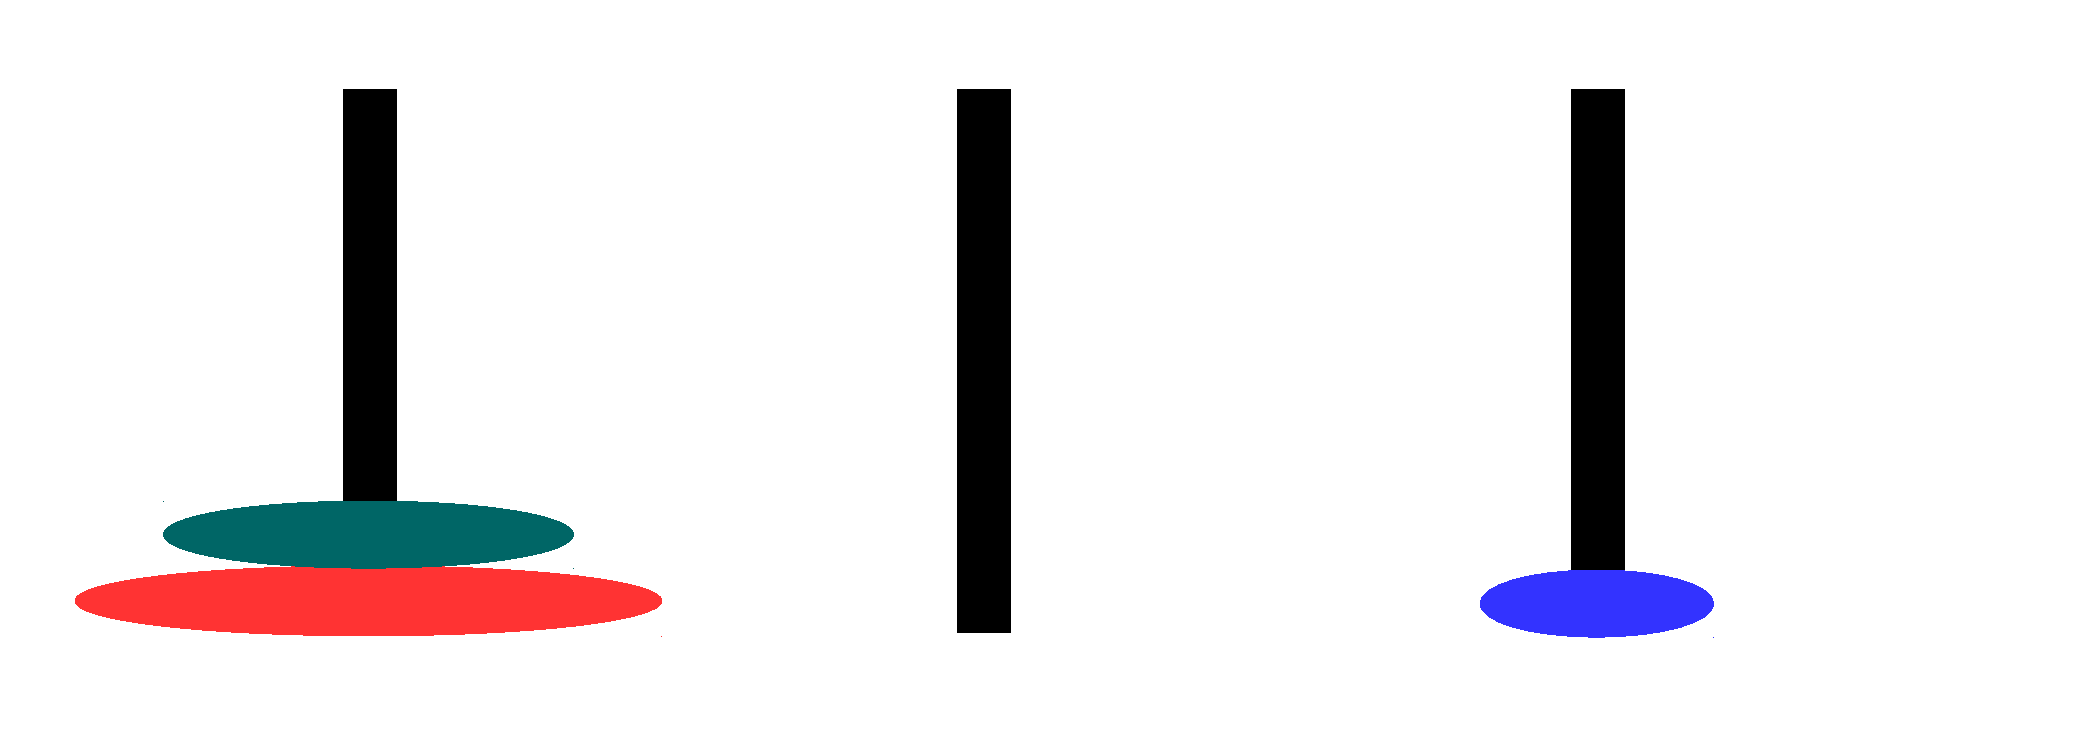
\includegraphics[width=11cm]{hanoi_solution1.pdf}%
\end{center}
}

\only<3>{
\begin{center}
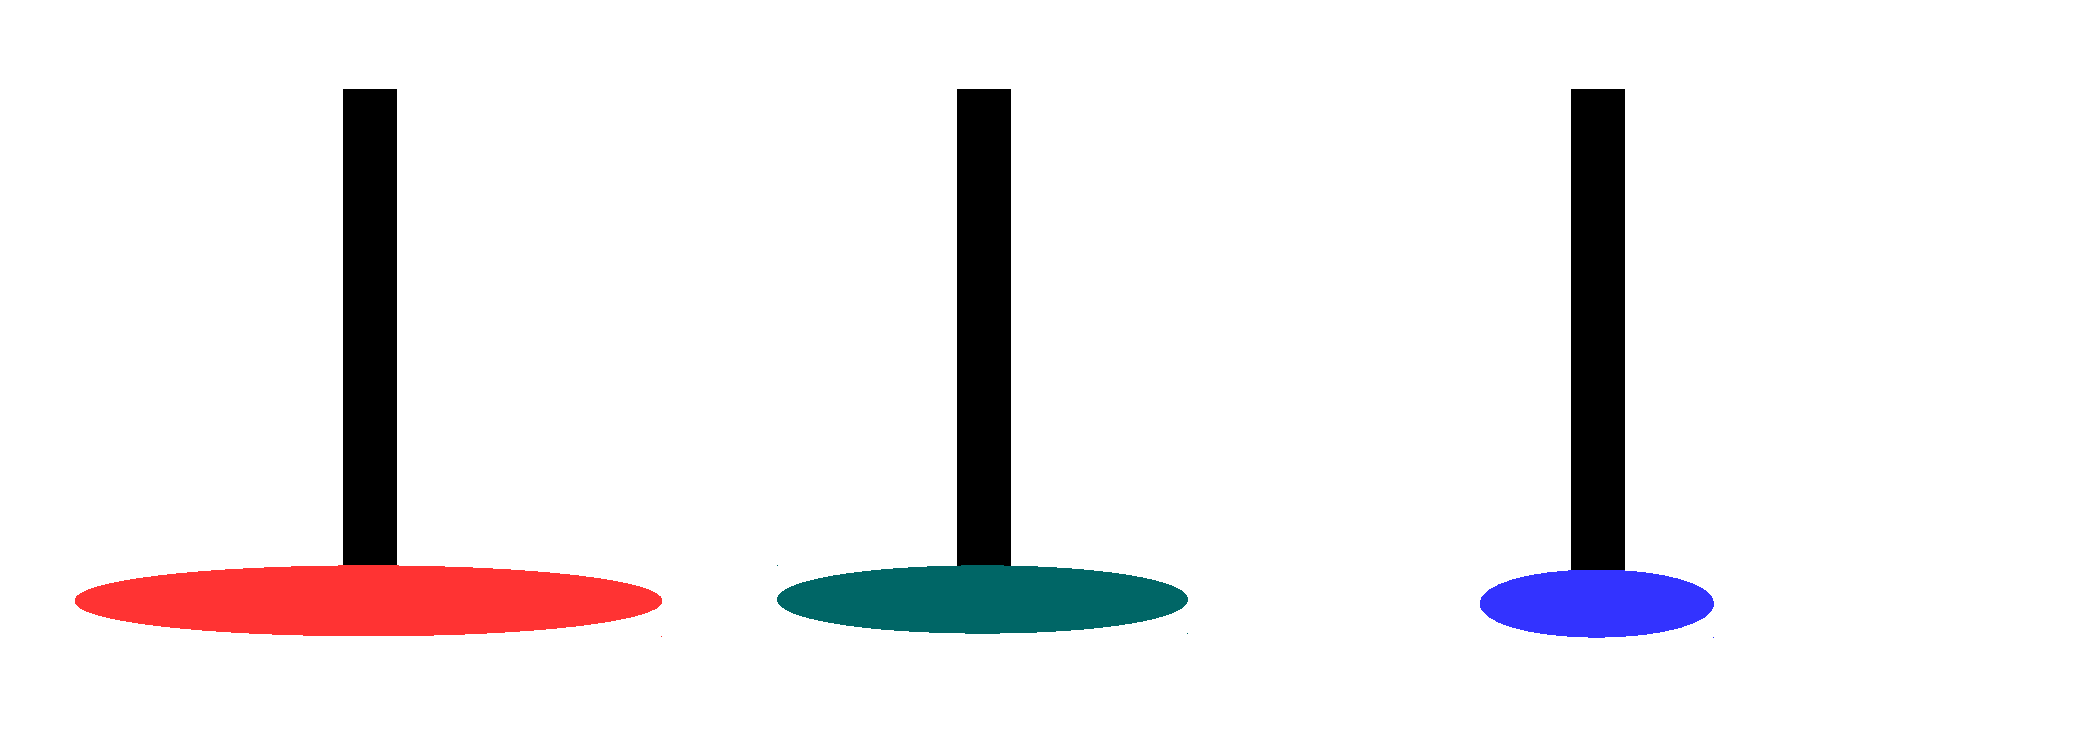
\includegraphics[width=11cm]{hanoi_solution2.pdf}%
\end{center}
}

\only<4>{
\begin{center}

\includegraphics[width=11cm]{hanoi_solution3.pdf}%
\end{center}
}

\only<5>{
\begin{center}

\includegraphics[width=11cm]{hanoi_solution4.pdf}%
\end{center}
}

\only<6>{
\begin{center}

\includegraphics[width=11cm]{hanoi_solution5.pdf}%
\end{center}
}

\only<7>{
\begin{center}
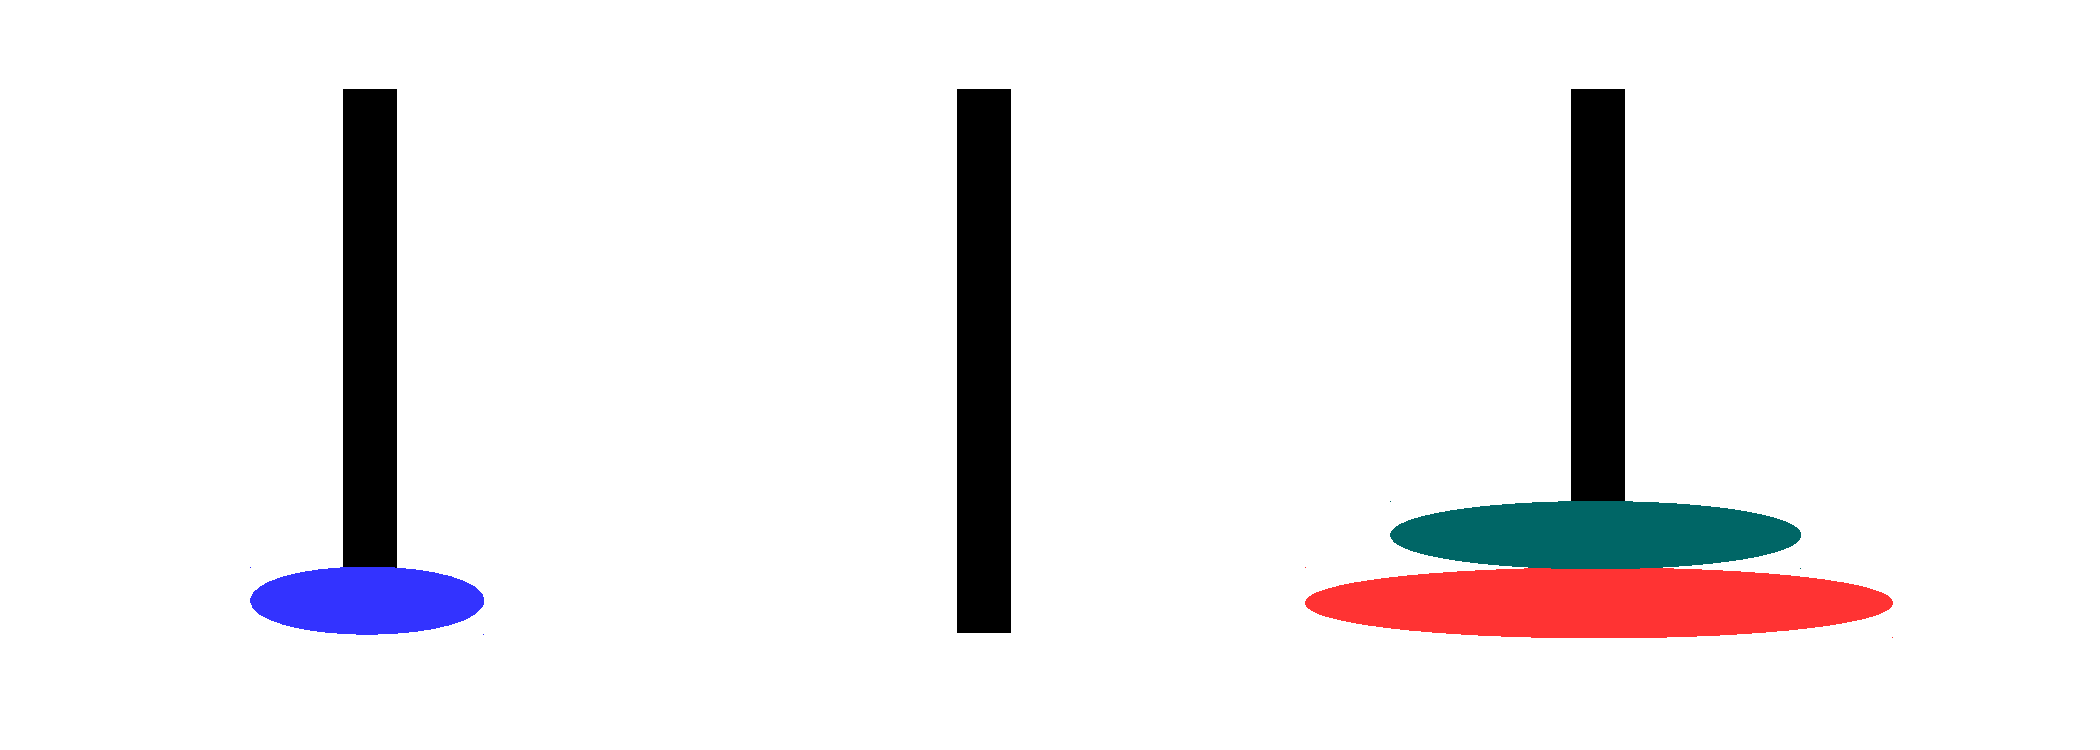
\includegraphics[width=11cm]{hanoi_solution6.pdf}%
\end{center}
}

\only<8>{
\begin{center}
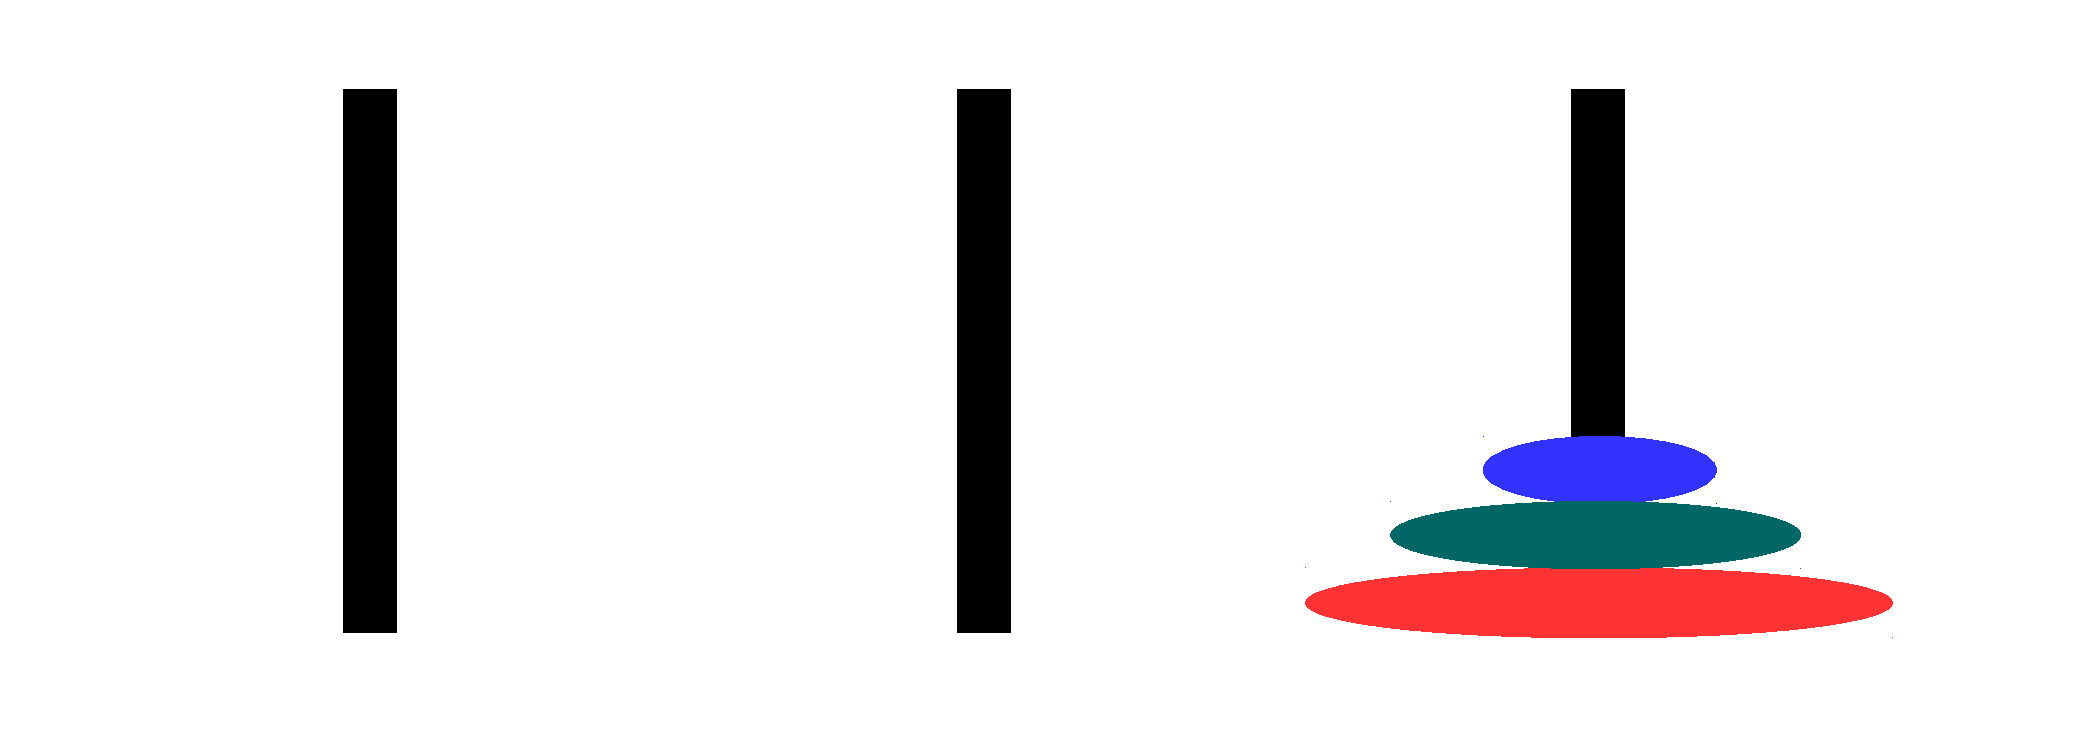
\includegraphics[width=11cm]{hanoi_solution7.pdf}%
\end{center}
}

\end{frame}

\begin{frame}[containsverbatim]
\frametitle{Solution: Base Case}

The \textbf{base case} is easy: Do nothing!

\begin{center}

\includegraphics[width=11cm]{hanoi_base_case.pdf}%
\end{center}

\end{frame}

\begin{frame}%[containsverbatim]
\frametitle{Solution: Inductive Case}

\textbf{Inductive case:} How to solve the problem for $n$ when you know how to solve it for $(n - 1)$?

\begin{center}
\includegraphics<1>[width=11cm]{hanoi_inductive_case.pdf}%
\includegraphics<2>[width=11cm]{hanoi_inductive_case1.pdf}%
\includegraphics<3>[width=11cm]{hanoi_inductive_case2.pdf}%
\includegraphics<4>[width=11cm]{hanoi_inductive_case3.pdf}%
\includegraphics<5>[width=11cm]{hanoi_inductive_case4.pdf}%
\end{center}

\end{frame}

\begin{frame}[containsverbatim]
\frametitle{Implementation}
\scriptsize
\begin{lstlisting}
void hanoi(int n,                      // Complexity: @$\textcolor{darkgreen}{O(2^n)}$@
           const string& start,
           const string& intermediate,
           const string& destination)
{
  if (n != 0)
  {
    hanoi(n - 1, start, destination, intermediate);
    cout << start << " --> " << destination << endl;
    hanoi(n - 1, intermediate, start, destination);
  }
}

int main(int argc, char *argv[]) { // A --> C
  hanoi(3, "A", "B", "C");         // A --> B
  return 0;                        // C --> B
                                   // A --> C
                                   // B --> A
                                   // B --> C
}                                  // A --> C
\end{lstlisting}

\end{frame}

\subsection{One-to-One Mappings}

\begin{frame}%[containsverbatim]
\frametitle{One-to-One Mappings}

\vspace{-0.7cm}
\begin{figure}
\centering
\begin{minipage}{0.6\textwidth}
\vspace{-1cm}
\begin{mdframed}[style=exampledefault, backgroundcolor=white]
\begin{itemize}
\item Let $f$ be a function that maps a finite set $A$ into itself.
\item In the diagram on the left
\begin{itemize}
\item $A = [0..6]$.
\item $f$ is represented by the edges.
\end{itemize}
\item The Problem: Find a subset $S\subseteq  A$ with the maximum number of elements, such that
\begin{itemize}
\item $f$ maps $S$ into itself.
\item $f$ is one-to-one when restricted to $S$.
\end{itemize}
\end{itemize}
\end{mdframed}
\end{minipage}~\begin{minipage}{0.4\textwidth}
\centering
\includegraphics<1>[width=4.7cm]{one_to_one_mappings.pdf}%
\includegraphics<2>[width=4.7cm]{one_to_one_mappings1.pdf}%
\includegraphics<3>[width=4.7cm]{one_to_one_mappings.pdf}%
\includegraphics<4>[width=4.7cm]{one_to_one_mappings2.pdf}%
\includegraphics<5>[width=4.7cm]{one_to_one_mappings3.pdf}%
\includegraphics<6>[width=4.7cm]{one_to_one_mappings4.pdf}%
\includegraphics<7>[width=4.7cm]{one_to_one_mappings5.pdf}%
\end{minipage}
\end{figure}

\end{frame}

\begin{frame}
\frametitle{Solution}

\begin{itemize}

\item The idea of a solution by induction is to concentrate on reducing the size of the problem.
\begin{itemize}
\item We can reduce the size by finding an element that belongs to $S$ or an element that does not belong to $S$.
\vspace{0.2cm}
\item We will reduce by finding an element that does not belong to $S$.
\end{itemize}
\vspace{0.5cm}
\item<2> We use the following \textbf{induction hypothesis:} We know how to solve the problem for sets of $(n - 1)$ elements.

\end{itemize}

\end{frame}

\begin{frame}[containsverbatim]
\frametitle{Solution: Base Case}

\textbf{Base case:} The set $A$ has only one element, so the function $f$ must map this element to itself.

\begin{center}
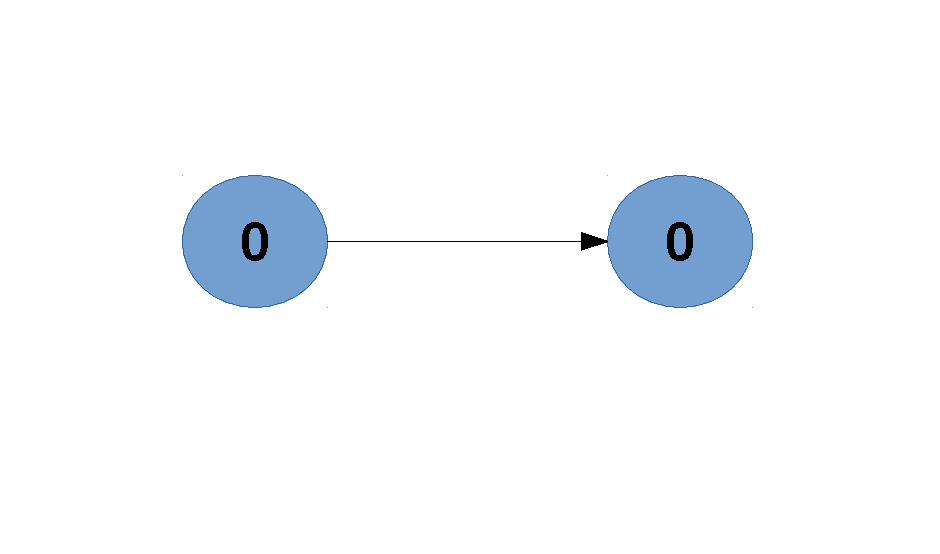
\includegraphics[width=8cm]{mappings_base_case.pdf}%
\end{center}

\end{frame}

\begin{frame}%[containsverbatim]
\frametitle{Solution: Inductive Case}

\begin{itemize}

\item<1-> \textbf{Inductive case:} If we can find an element $e \in A$ that does not belong to $S$, we can
\begin{itemize}

\item Set $A' = A - \{e\}$, and restrict $f$ to $A'$ to get $f' = f|_{A'}$.

\item Use the induction hypothesis on $A'$ and $f'$ to solve the problem.

\end{itemize}

\vspace{0.4cm}

\item<2-> We claim that any element $e$ that has no other element mapped to it cannot belong to $S$.
%% \begin{itemize}
%% \item If $e$ was in $S$, and $S$ has, say, $k$ elements, then
%% \begin{itemize}
%% \item Those $k$ elements are mapped into at most $k-1$ elements.
%% \item Therefore the mapping cannot be one-to-one.
%% \end{itemize}

\end{itemize}

\begin{center}
\begin{overlayarea}{0.4\textwidth}{0.6\textheight}
%\includegraphics<1>[width=3cm]{bijective_mappings_shadow.pdf}%
\includegraphics<2>[width=3cm]{bijective_mappings.pdf}%
\includegraphics<3>[width=3cm]{non_bijective_mappings.pdf}%
\end{overlayarea}
\end{center}

\end{frame}

\begin{frame}%[containsverbatim]
\frametitle{Solution: Example}

\vspace{-0.3cm}
\begin{center}
\includegraphics<1>[width=4.7cm]{one_to_one_mappings.pdf}%
\includegraphics<2>[width=4.7cm]{one_to_one_mappings_sol1.pdf}%
\includegraphics<3>[width=4.7cm]{one_to_one_mappings_sol2.pdf}%
\includegraphics<4>[width=4.7cm]{one_to_one_mappings_sol3.pdf}%
\includegraphics<5>[width=4.7cm]{one_to_one_mappings_sol4.pdf}%
\end{center}

\end{frame}


\begin{frame}[containsverbatim]
\frametitle{Solution: Implementation}

\scriptsize
\begin{lstlisting}
set<int> mapping(const vector<int>& f) { // Complexity: @$\textcolor{darkgreen}{O(\texttt{f.size()})}$@
  int initial_set_size = f.size();
  set<int> S;
  for (int i = 0; i < initial_set_size; ++i) { S.insert(i); }

  vector<int> counter(initial_set_size, 0);
  for (int i = 0; i < initial_set_size; ++i) { ++counter[f[i]]; }

  queue<int> q;
  for (int i = 0; i < initial_set_size; ++i) {
    if (counter[i] == 0) q.push(i);
  }
  while (!q.empty()) {
    int i = q.front(); q.pop();
    S.erase(i);
    --counter[f[i]];
    if (counter[f[i]] == 0) q.push(f[i]);
  }
  return S;
}
\end{lstlisting}

\end{frame}

\begin{frame}[containsverbatim]
\frametitle{Solution: Implementation}

\scriptsize
\begin{lstlisting}
int main(int argc, char *argv[])
{
  vector<int> f{2, 0, 0, 4, 4, 3, 5};
  auto res = mapping(f);
  for_each(res.begin(), res.end(),
          [&](int i) { cout << i << "->" << f[i] << endl; });
  return 0;
}
\end{lstlisting}

\begin{verbatim}
0->2
2->0
4->4
\end{verbatim}

\end{frame}

\subsection{Checking Containment}

\begin{frame}
\frametitle{Checking Intervals for Containment}
%\vspace{-0.7cm}
\begin{itemize}
\item The input is a set of intervals $I_1$, $I_2$, \ldots, $I_n$ on a line.

\item Each interval $I_j$ is given by its two end-points $L_j$ (left) and $R_j$ (right).

\item Problem: We want to mark all intervals that are contained in other intervals.

\end{itemize}

\begin{center}
\includegraphics<1>[width=9cm]{intervals_containment.pdf}%
\includegraphics<2>[width=9cm]{intervals_containment1.pdf}%
\end{center}

\end{frame}

\begin{frame}
\frametitle{Solution: First attempt}

\begin{itemize}

\item \textbf{Induction hypothesis:} We know how to solve the problem for $I_1$, $I_2$, \ldots, $I_{n-1}$.
\vspace{0.2cm}
\item We need to check $I_n$ against $(n-1)$ intervals.
\vspace{0.2cm}
\item Complexity: $(n-1) + (n-2) + \cdots + 1 = O(n^2)$.
\vspace{0.2cm}
\item<2> How to improve this?
\begin{itemize}
\item Choose a special interval to remove.
\item Gather more information from the solution of the smaller problem.
\end{itemize}

\end{itemize}

\end{frame}

\begin{frame}
\frametitle{Solution: Second attempt}

\begin{itemize}

\item Let $I$ be the interval with the largest (rightmost) left endpoint.
\begin{center}
\includegraphics<1>[width=9cm]{intervals_containment2.pdf}%
\includegraphics<2>[width=9cm]{intervals_containment3.pdf}%
\includegraphics<3>[width=9cm]{intervals_containment4.pdf}%
\includegraphics<4>[width=9cm]{intervals_containment5.pdf}%
\end{center}
\item<2-> There is no need to check left endpoint any further since all other intervals have smaller one.
\vspace{0.3cm}
\item<3-> We only need to check whether any other interval has a right endpoint larger than $I$'s right endpoint.

%\item<3> We sort the intervals according to their left endpoints.
%% \begin{itemize}
%% \item If for two intervals $I_j$, $I_k$ we have $L_j = L_k$, $I_j < I_k$ iff $R_j > R_k$.
%% \end{itemize}

%\item<2> Complexity: $O(n\log(n))$.

\end{itemize}

\end{frame}

\begin{frame}
\frametitle{Solution: Second attempt}

\vspace{-0.4cm}

\begin{center}
\includegraphics<1>[width=9cm]{intervals_containment.pdf}%
\includegraphics<2,3,4>[width=9cm]{intervals_containment6.pdf}%
\includegraphics<5>[width=9cm]{intervals_containment7.pdf}%
\includegraphics<6->[width=9cm]{intervals_containment8.pdf}%
\end{center}

\vspace{-0.8cm}
\begin{itemize}

\item<1-> We sort the intervals according to their left endpoints.
\begin{itemize}
\item<3-> Special case: If for two intervals $I_j$, $I_k$ we have $L_j = L_k$ then $I_j < I_k$ iff $R_j > R_k$.
\end{itemize}

\vspace{0.2cm}

\item<4-> \textbf{Stronger induction hypothesis:} We know how to solve the problem for $I_1$, $I_2$, \ldots, $I_{n-1}$ and
find the largest right endpoint (MaxR) among them.
\begin{itemize}

\item<5-> If MaxR $\ge R_n$ then $I_n$ should be marked, and MaxR doesn't change.

\item<6-> Otherwise (MaxR $< R_n$), $R_n$ becomes the new MaxR.

\end{itemize}
%\item<7> Complexity: $O(n\log(n))$.

\end{itemize}

\end{frame}

\begin{frame}[containsverbatim]
\frametitle{Solution: Implementation}

\scriptsize
\begin{lstlisting}
struct interval
{
  int index;
  int left;
  int right;
  bool operator<(const interval& i) const
  {
    return left < i.left || (left == i.left && right > i.right);
  }
};

ostream& operator<<(ostream& os, const interval& i)
{
  os << "[" << i.left << "," << i.right << "]";
  return os;
}
\end{lstlisting}

\end{frame}

\begin{frame}[containsverbatim]
\frametitle{Solution: Implementation}

\scriptsize
\begin{lstlisting}
// Let @$\textcolor{darkgreen}{n = \texttt{intervals.size()}}$@
// Complexity: @$\textcolor{darkgreen}{O(n\log(n))}$@
void interval_containment(vector<interval> intervals,
                          vector<bool>& marked)
{
  sort(intervals.begin(), intervals.end());
  int max_right = intervals[0].right;
  for (unsigned int i = 1; i < intervals.size(); ++i)
  {
    if (intervals[i].right <= max_right)
    {
      marked[intervals[i].index] = true;
    }
    else
    {
      max_right = intervals[i].right;
    }
  }
}
\end{lstlisting}

\end{frame}

\begin{frame}[containsverbatim]
\frametitle{Solution: Implementation}

\scriptsize
\begin{lstlisting}
int main(int argc, char *argv[])
{
  vector<interval> intervals{ {0,1,3}, {1,1,2}, {2,5,6}, {3,4,9},
                              {4,8,12} };
  vector<bool> marked(intervals.size(), false);
  interval_containment(intervals, marked);
  for (unsigned int i = 0; i < marked.size(); ++i)
  {
    if (marked[i]) cout << intervals[i] << endl;
  }
  return 0;
}
\end{lstlisting}

\begin{verbatim}
[1,2]
[5,6]
\end{verbatim}

\end{frame}

\subsection{Celebrity Problem}

\begin{frame}%[containsverbatim]
\frametitle{The Celebrity Problem}

\begin{figure}
\centering
\begin{minipage}{0.5\textwidth}
\begin{mdframed}[style=exampledefault, backgroundcolor=white]
Given an $n\times n$ adjacency matrix, determine if there exists an $i$ such that
\begin{itemize}
\item All the entries in the $i$th column are $1$.

\item All the entries in the $i$th row (except for the $ii$th entry) are $0$.

\end{itemize}
\end{mdframed}
\end{minipage}~\begin{minipage}{0.5\textwidth}
\centering
\begin{overlayarea}{0.8\textwidth}{0.6\textheight}
\only<1>{
\[
\begin{blockarray}{ccccccc}
& 0 & 1 & 2 & 3 & 4 \\
\begin{block}{c(cccccc)}
0 & 1 & 1 & 1 & 1 & 1 \\
1 & 0 & 1 & 1 & 0 & 1 \\
2 & 0 & 0 & 1 & 0 & 0 \\
3 & 0 & 0 & 1 & 1 & 1 \\
4 & 0 & 0 & 1 & 0 & 1 \\
\end{block}
\end{blockarray}
\]
}
\only<2>{
\[
\begin{blockarray}{ccccccc}
& 0 & 1 & \textcolor{orange}{2} & 3 & 4 \\
\begin{block}{c(cccccc)}
0 & 1 & 1 & \textcolor{orange}{1} & 1 & 1 \\
1 & 0 & 1 & \textcolor{orange}{1} & 0 & 1 \\
\textcolor{orange}{2} & \textcolor{orange}{0} & \textcolor{orange}{0} & \textcolor{orange}{1} & \textcolor{orange}{0} & \textcolor{orange}{0} \\
3 & 0 & 0 & \textcolor{orange}{1} & 1 & 1 \\
4 & 0 & 0 & \textcolor{orange}{1} & 0 & 1 \\
\end{block}
\end{blockarray}
\]
}
\end{overlayarea}
\end{minipage}
\end{figure}

\end{frame}

\begin{frame}%[containsverbatim]
\frametitle{\exo}

Design an algorithm to solve the celebrity problem. Using a clever reduction, you can obtain
an $O(n)$ complexity.

\end{frame}

\ifanswers

\begin{frame}
\frametitle{Solution}

\begin{itemize}

\item \textbf{Induction hypothesis:} We know how to solve the problem for $(n-1)$ persons.
\vspace{0.2cm}

\item<2-> \textbf{Base:} There is only two persons, we need to ask two questions.

\item<3-> \textbf{Reduction:} It is easy to indentify a noncelebrity. We ask a person $A$ if she knows $B$:
\begin{itemize}
\item<4-> If $A$ knows $B$ we can eliminate $A$.

\item<4-> Otherwise we eliminate $B$.
\end{itemize}

\vspace{0.2cm}

\item<5-> If there is a celebrity among the $(n-1)$ persons, it takes two more questions to check if this is a celebrity. Otherwise
there is no celebrity.

\item<6-> Complexity: $O(n)$.

\end{itemize}

\end{frame}

\begin{frame}[containsverbatim]
\frametitle{Solution: Implementation}

\scriptsize
\begin{lstlisting}
typedef vector<vector<int>> matrix;

int celebrity(const matrix& know) // Complexity: @$\textcolor{darkgreen}{O(\texttt{know.size()})}$@
{
  int n = know.size();
  int i = 0, j = 1;
  // In the first phase we eliminate all but one candidate
  for (int next = 2; next <= n; ++next)
  {
    if (know[i][j]) i = next;
    else j = next;
    // One of either i or j is eliminated
  }
  int candidate = i;
  if (i == n) candidate = j;
\end{lstlisting}

\end{frame}

\begin{frame}[containsverbatim]
\frametitle{Solution: Implementation}

\scriptsize
\begin{lstlisting}
  // Now we check that the candidate is indeed the celebrity
  for (int k = 0; k < n; ++k)
  {
    if (k != candidate && know[candidate][k])
    {
      return -1;
    }
    if (!know[k][candidate])
    {
      return -1;
    }
  }
  return candidate;
}
\end{lstlisting}

\end{frame}

\begin{frame}[containsverbatim]
\frametitle{Solution: Implementation}

\scriptsize
\begin{lstlisting}
int main(int argc, char *argv[])
{
  matrix know{ {1,1,1,1,1},
               {0,1,1,0,1},
               {0,0,1,0,0},
               {0,0,1,1,1},
               {0,0,1,0,1} };
  cout << celebrity(know) << endl;
  return 0;
}
\end{lstlisting}

\begin{verbatim}
2
\end{verbatim}

\end{frame}

\fi

\subsection{The Skyline Problem}

\begin{frame}%[containsverbatim]
\frametitle{The Skyline Problem}

\begin{mdframed}[style=exampledefault]
Problem: Given the exact locations and shapes of several rectangular buildings in a city,
draw the skyline (in 2D) of these buildings, eliminating hidden lines.
\end{mdframed}

\begin{center}
\includegraphics<1>[width=9.5cm]{skyline.pdf}%
\includegraphics<2>[width=9.5cm]{skyline1.pdf}%
\end{center}

\end{frame}

\begin{frame}
\frametitle{Solution: First Attempt}

\begin{itemize}

\item \textbf{Induction hypothesis:} We know how to solve the problem for $(n-1)$ buildings.
\vspace{0.2cm}
\item We need to add the $n^{\textrm{th}}$ building to the skyline.

\begin{center}
\begin{overlayarea}{0.8\textwidth}{0.6\textheight}
\includegraphics<2>[width=9.5cm]{skyline2.pdf}%
\includegraphics<3>[width=9.5cm]{skyline3.pdf}%
\includegraphics<4->[width=9.5cm]{skyline4.pdf}%
\end{overlayarea}
\end{center}

\visible<5>{
\vspace{-0.5cm}
\item Complexity: $O(n^2)$.}

\end{itemize}

\end{frame}

\begin{frame}
\frametitle{Solution: Second Attempt}

\begin{itemize}

\item \textbf{Stronger induction hypothesis:} We know how to solve the problem for $k$ buildings where $k < n$.
\vspace{0.2cm}
\item<2-> We split the buildings in two sets of $\frac{n}{2}$ elements which we can solve inductively.
\vspace{0.2cm}
\item<3-> We get two skylines. It remains to merge them efficiently.

\end{itemize}

\begin{overlayarea}{0.95\textwidth}{0.6\textheight}
\begin{center}
\includegraphics<4>[width=5.5cm]{skyline.pdf}%
\includegraphics<5>[width=5.5cm]{skyline5.pdf}%
\includegraphics<6>[width=5.5cm]{skyline6.pdf}%
\includegraphics<7>[width=10cm]{skyline7.pdf}%
\includegraphics<8>[width=10cm]{skyline8.pdf}%
\includegraphics<9>[width=10cm]{skyline9.pdf}%
\includegraphics<10>[width=10cm]{skyline10.pdf}%
\includegraphics<11>[width=10cm]{skyline11.pdf}%
\includegraphics<12>[width=10cm]{skyline12.pdf}%
\includegraphics<13>[width=10cm]{skyline13.pdf}%
\includegraphics<14>[width=10cm]{skyline14.pdf}%
\includegraphics<15>[width=10cm]{skyline15.pdf}%
\includegraphics<16>[width=10cm]{skyline16.pdf}%
\includegraphics<17>[width=10cm]{skyline17.pdf}%
\includegraphics<18>[width=10cm]{skyline18.pdf}%
\includegraphics<19>[width=10cm]{skyline19.pdf}%
\includegraphics<20>[width=10cm]{skyline20.pdf}%
\includegraphics<21>[width=10cm]{skyline21.pdf}%
\includegraphics<22>[width=10cm]{skyline22.pdf}%
\includegraphics<23>[width=10cm]{skyline23.pdf}%
\includegraphics<24>[width=10cm]{skyline24.pdf}%
\includegraphics<25>[width=10cm]{skyline25.pdf}%
\end{center}
%\includegraphics<4->[width=9.5cm]{skyline7.pdf}%
\end{overlayarea}

\end{frame}

\begin{frame}[containsverbatim]
\frametitle{Solution: Implementation}

\scriptsize
\begin{lstlisting}
struct building
{
  int left;
  int right;
  int height;
};

struct strip
{
  int left;
  int height;
};

ostream& operator<<(ostream& os, const strip& s)
{
  os << "(left: " << s.left << ", height: " << s.height << ")";
  return os;
}
\end{lstlisting}

\end{frame}

\begin{frame}[containsverbatim]
\frametitle{Solution: Implementation}

\scriptsize
\begin{lstlisting}
// Let @$\textcolor{darkgreen}{n = \texttt{buildings.size()}}$@
// Complexity: @$\textcolor{darkgreen}{O(n\log(n))}$@
vector<strip> skyline(const vector<building>& buildings,
                      int low, int high)
{
  if (low == high)
  {
    building b = buildings[low];
    return { {b.left, b.height}, {b.right, 0} };
  }

  int middle = low + (high - low) / 2;

  vector<strip> first  = skyline(buildings, low, middle);
  vector<strip> second = skyline(buildings, middle + 1, high);

  return merge(first, second);
}
\end{lstlisting}
\end{frame}

\begin{frame}[containsverbatim]
\frametitle{Solution: Implementation}

\scriptsize
\begin{lstlisting}
vector<strip> merge(const vector<strip>& first,
                    const vector<strip>& second)
 {
  vector<strip> res;
  unsigned int i = 0, j = 0;
  int h1 = 0, h2 = 0;
  while (i < first.size() && j < second.size())
  {
    if (first[i].left < second[j].left) {
      h1 = first[i].height;
      append(res, {first[i].left, max(h1, h2)});
      ++i;
    } else {
      h2 = second[j].height;
      append(res, {second[j].left, max(h1, h2)});
      ++j;
    }
  }
  // ...
\end{lstlisting}
\end{frame}

\begin{frame}[containsverbatim]
\frametitle{Solution: Implementation}

\scriptsize
\begin{lstlisting}
  // ...
  while (i < first.size())
  {
    append(res, first[i]);
    ++i;
  }
  while (j < second.size())
  {
    append(res, second[j]);
    ++j;
  }
  return res;
}
\end{lstlisting}
\end{frame}

\begin{frame}[containsverbatim]
\frametitle{Solution: Implementation}

\scriptsize
\begin{lstlisting}
void append(vector<strip>& skyline, const strip& s)
{
  if (skyline.size() == 0)
  {
    skyline.push_back(s);
    return;
  }
  int last_index = skyline.size() - 1;
  strip last = skyline[last_index];
  if (last.left == s.left || last.height == s.height)
  {
    skyline[last_index] = {last.left, max(last.height, s.height)};
  }
  else
  {
    skyline.push_back(s);
  }
}
\end{lstlisting}
\end{frame}

\begin{frame}[containsverbatim]
\frametitle{Solution: Implementation}

\scriptsize
\begin{lstlisting}
vector<strip> skyline(const vector<building>& buildings)
{
  vector<strip> res = skyline(buildings, 0, buildings.size() - 1);
  res.back().height = 0;
  return res;
}
\end{lstlisting}

\end{frame}

\begin{frame}[containsverbatim]
\frametitle{Solution: Implementation}

\scriptsize
\begin{lstlisting}
int main(int argc, char *argv[])
{
  vector<building> buildings {
    {3,9,13}, {12,16,7}, {14,25,3}, {1,5,11}, {2,7,6}, {19,22,18},
    {23,29,13}, {24,28,4}
  };
  vector<strip> res = skyline(buildings);
  copy(res.begin(), res.end(), ostream_iterator<strip>(cout, "\n"));
  return 0;
}
\end{lstlisting}

\begin{verbatim}
(left: 1, height: 11)
(left: 3, height: 13)
(left: 9, height: 0)
(left: 12, height: 7)
(left: 16, height: 3)
(left: 19, height: 18)
(left: 22, height: 3)
(left: 23, height: 13)
(left: 29, height: 0)
\end{verbatim}

\end{frame}

\subsection{Maximum Subsequence}

\begin{frame}%[containsverbatim]
\frametitle{The Maximum Consecutive Subsequence}

\begin{mdframed}[style=exampledefault]
Problem: Given a sequence $x_1, x_2, \ldots, x_n$ of real numbers, find a
subsequence $x_i, x_{i+1}, \ldots, x_j$ (of consecutive elements) such that the sum of the numbers in it is
maximum over all subsequences of consecutive elements.
\end{mdframed}

\begin{center}
\includegraphics<1>[width=12cm]{maximum_consecutive_subsequence.pdf}%
\includegraphics<2>[width=12cm]{maximum_consecutive_subsequence1.pdf}%
\end{center}

\end{frame}

\begin{frame}%[containsverbatim]
\frametitle{\exo}

Design an algorithm, with a linear time complexity, to solve the maximum consecutive subsequence problem.

\end{frame}

\ifanswers

\begin{frame}
\frametitle{Solution: First Attempt}

\begin{itemize}

\item \textbf{Induction hypothesis:} We know how to solve the problem for any array of $(n-1)$ elements.
\vspace{0.2cm}
\item If we have the maximum consecutive subsequence for the array of $(n-1)$ elements, how to extend it with the
$n^{\textrm{th}}$ element?

\begin{center}
\begin{overlayarea}{1\textwidth}{0.2\textheight}
\includegraphics<2>[width=12cm]{maximum_consecutive_subsequence2.pdf}%
\includegraphics<3>[width=12cm]{maximum_consecutive_subsequence3.pdf}%
\includegraphics<4>[width=12cm]{maximum_consecutive_subsequence4.pdf}%
\includegraphics<5>[width=12cm]{maximum_consecutive_subsequence5.pdf}%
\end{overlayarea}
\end{center}

\end{itemize}

\end{frame}

\begin{frame}
\frametitle{Solution: Second Attempt}

\begin{itemize}

\item \textbf{Stronger induction hypothesis:} We know how to solve the problem for any array of $(n-1)$ elements and get
the maximum subsequence that is a suffix.
\vspace{0.2cm}

\item<2-> \textbf{Base case:} The array is empty:
\begin{itemize}
\item The maximum subsequence is $0$.
\item The maximum suffix is $0$.
\end{itemize}

\item<3-> If we have the maximum consecutive subsequence and suffix for the array of $(n-1)$ elements, how to extend it with the
$n^{\textrm{th}}$ element?

\begin{center}
\begin{overlayarea}{1\textwidth}{0.2\textheight}
\includegraphics<3>[width=12cm]{maximum_consecutive_subsequence6.pdf}%
\includegraphics<4>[width=12cm]{maximum_consecutive_subsequence7.pdf}%
\includegraphics<5>[width=12cm]{maximum_consecutive_subsequence8.pdf}%
\includegraphics<6>[width=12cm]{maximum_consecutive_subsequence9.pdf}%
\end{overlayarea}
\end{center}

\end{itemize}

\end{frame}

\begin{frame}[containsverbatim]
\frametitle{Solution: Implementation}

\scriptsize
\begin{lstlisting}
// Complexity: @$\textcolor{darkgreen}{O(\texttt{sequence.size()})}$@
// If @\textcolor{darkgreen}{\texttt{sequence}}@ contains only negative values, returns @$\textcolor{darkgreen}{0}$@
double maximum_consecutive_subsequence(vector<double> sequence) {
  double global_max = 0;
  double suffix_max = 0;
  for (unsigned int i = 0; i < sequence.size(); ++i)
  {
    if (sequence[i] + suffix_max > global_max)
    {
      suffix_max += sequence[i];
      global_max = suffix_max;
    }
    else
    {
      if (sequence[i] + suffix_max > 0) suffix_max += sequence[i];
      else suffix_max = 0;
    }
  }
  return global_max;
}
\end{lstlisting}
\end{frame}

\begin{frame}[containsverbatim]
\frametitle{Solution: Implementation}

\scriptsize
\begin{lstlisting}
int main(int argc, char *argv[])
{
  vector<double> sequence{2,0,-4,1,3,-1,-2,2,5,0,1,-20,8,-8,2};
  cout << maximum_consecutive_subsequence(sequence) << endl;
  return 0;
}
\end{lstlisting}

\begin{verbatim}
9
\end{verbatim}

\end{frame}

\begin{frame}[containsverbatim]
\frametitle{Solution: Implementation}

\scriptsize
\begin{lstlisting}
// Complexity: @$\textcolor{darkgreen}{O(\texttt{sequence.size()})}$@
// If @\textcolor{darkgreen}{\texttt{sequence}}@ contains only negative values, returns the max of them
double maximum_consecutive_subsequence(vector<double> sequence)
{
  double global_max = sequence[0];
  double suffix_max = max(global_max, 0.);
  for (unsigned int i = 1; i < sequence.size(); ++i)
    {
      double v = sequence[i];
      suffix_max += v;
      global_max = max(global_max, suffix_max);
      if (suffix_max < 0) suffix_max = 0;
    }
  return global_max;
}
\end{lstlisting}
\end{frame}

\fi

\subsection{Tiling}

\begin{frame}%[containsverbatim]
\frametitle{Tiling Problem}

\begin{mdframed}[style=exampledefault]
Problem: In how many ways can you tile a $3\times n$ rectangle with $2\times 1$ dominoes? (\spojlink{M3tile}{http://www.spoj.com/problems/M3TILE/})
\end{mdframed}

\begin{overlayarea}{1\textwidth}{0.7\textheight}
\begin{center}
\includegraphics<2>[width=8cm]{tiling_3xn.pdf}%
\includegraphics<3>[width=8cm]{tiling_3xn_1.pdf}%
\end{center}
\end{overlayarea}

\end{frame}

\begin{frame}%[containsverbatim]
\frametitle{\exo}

How to reduce a $3\times n$ rectangle to other shapes to solve the problem by induction?

\end{frame}


\tikzset{
    invisible/.style={opacity=0,text opacity=0},
    visible on/.style={alt={#1{}{invisible}}},
    alt/.code args={<#1>#2#3}{%
      \alt<#1>{\pgfkeysalso{#2}}{\pgfkeysalso{#3}} % \pgfkeysalso doesn't change the path
    },
  }

\newenvironment{mytikz}[1][]{\begin{tikzpicture}[#1]}{\end{tikzpicture}}

\ifanswers

\begin{frame}%[containsverbatim]
\frametitle{Subproblems}

\footnotesize

\setbeamercovered{transparent=0}

We fill the last column of the rectangle, and see what the remaining shape is. We can obtain the following shapes:

\vspace{0.75cm}

\begin{center}
\begin{tikzpicture}[x=0.5cm, y=0.5cm]
\draw (2.5,3) node[above]{$\text{Flat}_n$};
\draw (0,0) rectangle (4,3);
\draw[fill=blue!40!white, dashed] (4,2) rectangle (6,3);
\draw[fill=blue!40!white, dashed] (4,1) rectangle (6,2);
\draw[fill=blue!40!white, dashed] (4,0) rectangle (6,1);
\end{tikzpicture}
%\vspace{0.5cm}
\begin{tikzpicture}[x=0.5cm, y=0.5cm]
\draw (2.5,3) node[above]{$\text{W/oTop}_n$};
\draw (0,0) -- (5,0) -- (5,2) -- (4,2) -- (4,3) -- (0,3) -- cycle;
\draw[fill=blue!40!white, dashed] (4,2) rectangle (6,3);
\draw[fill=blue!40!white, dashed] (5,0) rectangle (6,2);
\end{tikzpicture}
%\vspace{0.5cm}
\begin{tikzpicture}[x=0.5cm, y=0.5cm]
\draw (2.5,3) node[above]{$\text{W/oBottom}_n$};
\draw (0,0) -- (4,0) -- (4,1) -- (5,1) -- (5,3) -- (0,3) -- cycle;
\draw[fill=blue!40!white, dashed] (5,1) rectangle (6,3);
\draw[fill=blue!40!white, dashed] (4,0) rectangle (6,1);
\end{tikzpicture}
\end{center}

\end{frame}

\begin{frame}%[containsverbatim]
\frametitle{Subproblems}

\footnotesize

\setbeamercovered{transparent=0}

Now, from

\vspace{0.5cm}

\begin{center}
\begin{tikzpicture}[x=0.5cm, y=0.5cm]
\draw (2.5,3) node[above]{$\text{W/oTop}_n$};
\draw (0,0) -- (5,0) -- (5,2) -- (4,2) -- (4,3) -- (0,3) -- cycle;
\end{tikzpicture}~\hspace{2cm}~\begin{tikzpicture}[x=0.5cm, y=0.5cm]
\draw (2.5,3) node[above]{$\text{W/oBottom}_n$};
\draw (0,0) -- (4,0) -- (4,1) -- (5,1) -- (5,3) -- (0,3) -- cycle;
\end{tikzpicture}
\end{center}

\onslide<2->
\vspace{0.5cm}
We fill again the last column to get,
\vspace{0.5cm}

\begin{overlayarea}{1\textwidth}{0.5\textheight}
\begin{center}

\begin{tikzpicture}[x=0.4cm, y=0.4cm]
\draw (2.5,3) node[above]{$\text{Flat}_n$};
\draw (0,0) -- (5,0) -- (5,2) -- (4,2) -- (4,3) -- (0,3) -- cycle;
\draw[fill=blue!40!white, dashed] (4,0) rectangle (5,2);
\end{tikzpicture}~\hspace{0.1cm}~\begin{tikzpicture}[x=0.4cm, y=0.4cm]
\draw (2.5,3) node[above]{$\text{W/oMiddle\&Bottom}_n$};
\draw (0,0) -- (5,0) -- (5,2) -- (4,2) -- (4,3) -- (0,3) -- cycle;
\draw[fill=blue!40!white, dashed] (3,0) rectangle (5,1);
\draw[fill=blue!40!white, dashed] (3,1) rectangle (5,2);
\end{tikzpicture}~\hspace{0.1cm}~\begin{tikzpicture}[x=0.4cm, y=0.4cm]
\draw (2.5,3) node[above]{$\text{Flat}_n$};
\draw (0,0) -- (4,0) -- (4,1) -- (5,1) -- (5,3) -- (0,3) -- cycle;
\draw[fill=blue!40!white, dashed] (4,1) rectangle (5,3);
\end{tikzpicture}~\hspace{0.1cm}~\begin{tikzpicture}[x=0.4cm, y=0.4cm]
\draw (2.5,3) node[above]{$\text{W/oTop\&Middle}_n$};
\draw (0,0) -- (4,0) -- (4,1) -- (5,1) -- (5,3) -- (0,3) -- cycle;
\draw[fill=blue!40!white, dashed] (3,1) rectangle (5,2);
\draw[fill=blue!40!white, dashed] (3,2) rectangle (5,3);
\end{tikzpicture}
\end{center}

\end{overlayarea}


\end{frame}

\begin{frame}%[containsverbatim]
\frametitle{Subproblems}

\footnotesize

\setbeamercovered{transparent=0}

And finally, from

\vspace{0.5cm}

\begin{center}
\begin{tikzpicture}[x=0.5cm, y=0.5cm]
\draw (2.5,3) node[above]{$\text{W/oMiddle\&Bottom}_n$};
\draw (0,0) -- (4,0) -- (4,2) -- (5,2) -- (5,3) -- (0,3) -- cycle;
\end{tikzpicture}~\hspace{2cm}~\begin{tikzpicture}[x=0.5cm, y=0.5cm]
\draw (2.5,3) node[above]{$\text{W/oTop\&Middle}_n$};
\draw (0,0) -- (5,0) -- (5,1) -- (4,1) -- (4,3) -- (0,3) -- cycle;
\end{tikzpicture}
\end{center}

\onslide<2->
\vspace{0.5cm}
We fill again the last column to get some shapes we have already seen:
\vspace{0.5cm}

\begin{overlayarea}{1\textwidth}{0.5\textheight}
\begin{center}
\begin{tikzpicture}[x=0.5cm, y=0.5cm]
\draw (2.5,3) node[above]{$\text{W/oTop}_n$};
\draw (0,0) -- (4,0) -- (4,2) -- (5,2) -- (5,3) -- (0,3) -- cycle;
\draw[fill=blue!40!white, dashed] (3,2) rectangle (5,3);
\end{tikzpicture}~\hspace{1cm}~\begin{tikzpicture}[x=0.5cm, y=0.5cm]
\draw (2.5,3) node[above]{$\text{W/oBottom}_n$};
\draw (0,0) -- (5,0) -- (5,1) -- (4,1) -- (4,3) -- (0,3) -- cycle;
\draw[fill=blue!40!white, dashed] (3,0) rectangle (5,1);
\end{tikzpicture}
\end{center}

\end{overlayarea}

\end{frame}

\begin{frame}%[containsverbatim]
\frametitle{Equations}

\setbeamercovered{transparent=0}

\begin{itemize}

\item If $n = 0$, there is only one possible tiling.

\vspace{0.4cm}

\item<2-> If $n = 1$, there is one possible tiling iff we are in the configurations $\text{W/oTop}_1$ or $\text{W/oBottom}_1$.

\vspace{0.4cm}

\item<3-> $\text{Flat}_n = \text{Flat}_{n-2} + \text{W/oTop}_{n-1} + \text{W/oBottom}_{n-1}$.

\vspace{0.4cm}

\item<4-> $\text{W/oTop}_{n} = \text{Flat}_{n-1} + \text{W/oMiddle\&Bottom}_{n-1}$.

\vspace{0.4cm}

\item<5-> $\text{W/oBottom}_{n} = \text{Flat}_{n-1} + \text{W/oTop\&Middle}_{n-1}$.

\vspace{0.4cm}

\item<6-> $\text{W/oMiddle\&Bottom}_{n} = \text{W/oTop}_{n-1}$.

\vspace{0.4cm}

\item<7-> $\text{W/oTop\&Middle}_{n} = \text{W/oBottom}_{n-1}$.

\end{itemize}

\end{frame}

\begin{frame}[containsverbatim]
\frametitle{Solution Implementation}

\scriptsize
\begin{lstlisting}
enum { FLAT = 0, WITHOUT_TOP = 1,
       WITHOUT_MIDDLE = 2, WITHOUT_BOTTOM = 4 };

long long memo[32][8];

long long tile(int n, int configuration);

int main(int argc, char *argv[])
{
  int N;
  memset(memo, -1, sizeof memo);
  while (cin >> N && N != -1)
  {
    cout << tile(N, FLAT) << endl;
  }
  return 0;
}
\end{lstlisting}

\end{frame}

\begin{frame}[containsverbatim]
\frametitle{Solution Implementation}

\scriptsize
\begin{lstlisting}
long long tile(int n, int configuration) {
  if (n == 0) return 1;
  if (n == 1) return configuration == WITHOUT_TOP ||
                     configuration == WITHOUT_BOTTOM;
  long long& res = memo[n][configuration];
  if (res != -1) return res;
  res = 0;
  if (configuration == FLAT) {
    res = tile(n - 2, FLAT) + 2 * tile(n - 1, WITHOUT_TOP);
  }
  else if (configuration == WITHOUT_TOP) {
    res = tile(n - 1, FLAT) +
          tile(n - 1, WITHOUT_MIDDLE | WITHOUT_BOTTOM);
  }
  else if (configuration == (WITHOUT_MIDDLE | WITHOUT_BOTTOM)) {
    res = tile(n - 1, WITHOUT_TOP);
  }
  return res;
}
\end{lstlisting}

\end{frame}

\fi

\subsection{Common Errors}

\begin{frame}%[containsverbatim]
\frametitle{Common Errors}

\begin{itemize}

\item Forgetting the base case.

\vspace{0.5cm}

\item<2-> Extend a solution for $(n-1)$ to a solution of a special instance
of the problem for $n$.

\vspace{0.5cm}

\item<3-> Changing the hypothesis unintentionally.

\end{itemize}

\end{frame}

\begin{frame}%[containsverbatim]
\frametitle{Common Error: Changing the Hypothesis}

\scriptsize

\begin{block}{Definition}
A graph $G = (V, E)$ is called \textbf{bipartite} if its set of vertices can be partitioned into two subsets
such that there is no edge connecting two vertices from the same subset.
\end{block}

\begin{overlayarea}{1\textwidth}{0.5\textheight}
\begin{center}
\includegraphics<1>[width=5cm]{bipartite.pdf}%
\includegraphics<2->[width=5cm]{bipartite1.pdf}%
\end{center}
\end{overlayarea}

\onslide<3>
\begin{block}{Property}
If a graph is connected and bipartite, then the partition is unique.
\end{block}

\end{frame}


\begin{frame}%[containsverbatim]
\frametitle{Common Error: Changing the Hypothesis}

\begin{mdframed}[style=exampledefault]
Problem: Given a connected undirected graph $G = (V, E)$, determine whether it is bipartite and, if it is, partition
the vertices accordingly.
\end{mdframed}

\vspace{0.5cm}
\onslide<2->
\textbf{A Wrong solution.}

\begin{itemize}

\item Remove a vertex $v$ and partition the rest of the graph, if possible, by induction.
\begin{itemize}
\item We call the first subset \textcolor{red}{red} and the second \textcolor{blue}{blue}.
\end{itemize}

\item<3-> If $v$ is connected to only blue vertices, add it to the \textcolor{red}{red} subset.

\item<4-> If $v$ is connected to only red vertices, add it to the \textcolor{blue}{blue} subset.

\item<5-> Otherwise, the graph is not bipartite (since the partition is unique).

\end{itemize}

\end{frame}

\begin{frame}%[containsverbatim]
\frametitle{\exo}

What is wrong with the previous solution?

\end{frame}

\ifanswers

\begin{frame}%[containsverbatim]
\frametitle{Solution}

When we remove the vertex $v$, the subgraph can become disconnected.

\begin{center}
\begin{figure}
\includegraphics<1>[width=6cm]{bipartite.pdf}%
\includegraphics<2>[width=6cm]{bipartite2.pdf}%
\includegraphics<3>[width=6cm]{bipartite3.pdf}%
\includegraphics<4>[width=6cm]{bipartite4.pdf}%
\end{figure}
\end{center}

\end{frame}

\fi

\subsection{Exercices}

\begin{frame}%[containsverbatim]
\frametitle{\exo}

This exercice is a variation of the towers of Hanoi problem. We no longer
assume that all the disks are initially on one peg. They may be distributed among the three pegs, as long as they are ordered
in decreasing sizes on each peg.

\begin{figure}
\centering
\begin{minipage}{0.5\textwidth}
\centering
\vspace{1cm}
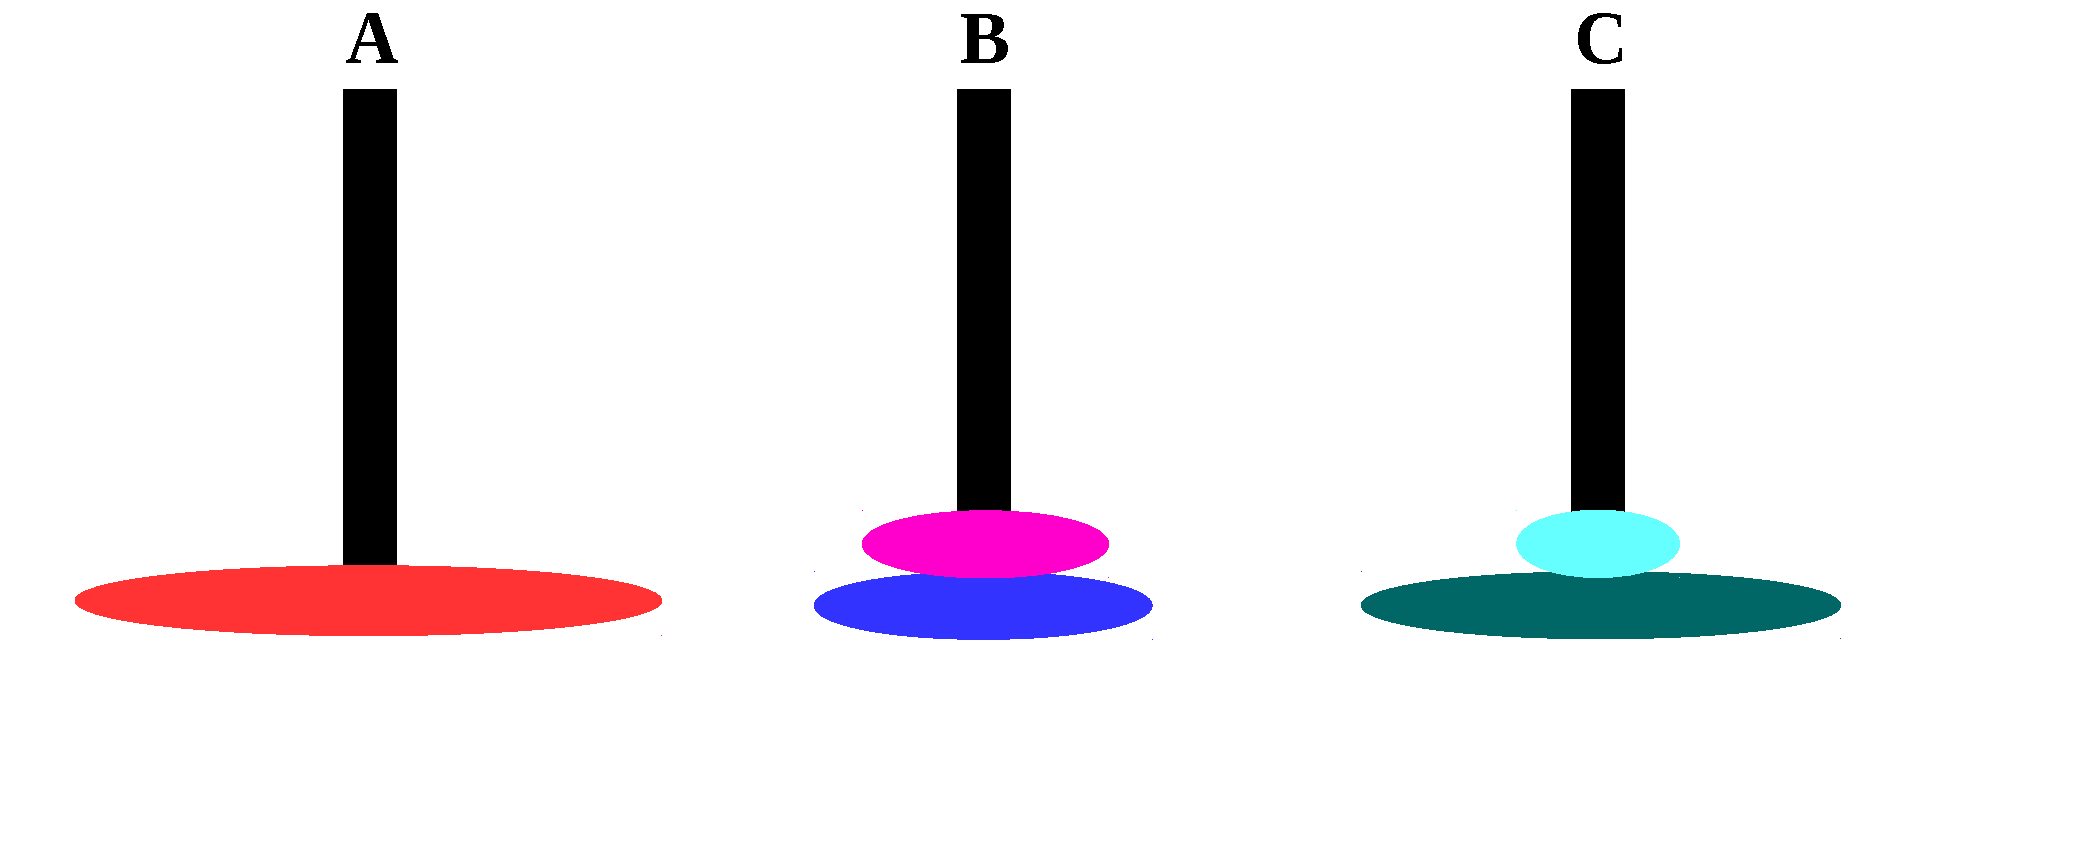
\includegraphics[width=6cm]{hanoi_exo.pdf}%
\end{minipage}~\begin{minipage}{0.5\textwidth}
\centering
\begin{overlayarea}{0.7\textwidth}{0.4\textheight}
{\fontsize{8}{8}\selectfont
\texttt{C$\rightarrow$A}
\texttt{B$\rightarrow$C}
\texttt{A$\rightarrow$C}
\texttt{B$\rightarrow$A}
\texttt{C$\rightarrow$B}\\
\vspace{0.3cm}
\texttt{C$\rightarrow$A}
\texttt{B$\rightarrow$A}
\texttt{C$\rightarrow$B}
\texttt{A$\rightarrow$B}
\texttt{A$\rightarrow$C}\\
\vspace{0.3cm}
\texttt{B$\rightarrow$C}
\texttt{A$\rightarrow$B}
\texttt{C$\rightarrow$A}
\texttt{C$\rightarrow$B}
\texttt{A$\rightarrow$B}\\
\vspace{0.3cm}
\texttt{A$\rightarrow$C}
\texttt{B$\rightarrow$A}
\texttt{B$\rightarrow$C}
\texttt{A$\rightarrow$C}
\texttt{B$\rightarrow$A}\\
\vspace{0.3cm}
\texttt{C$\rightarrow$B}
\texttt{C$\rightarrow$A}
\texttt{B$\rightarrow$A}
\texttt{B$\rightarrow$C}
\texttt{A$\rightarrow$C}\\
\vspace{0.3cm}
\texttt{A$\rightarrow$B}
\texttt{C$\rightarrow$B}
\texttt{A$\rightarrow$C}
\texttt{B$\rightarrow$A}
\texttt{B$\rightarrow$C}\\
\vspace{0.1cm}
\texttt{A$\rightarrow$C} ($31$ moves).}
\end{overlayarea}
\end{minipage}
\end{figure}

\begin{center}

\end{center}

\end{frame}

\ifanswers

\begin{frame}[containsverbatim]
\frametitle{Solution: Implementation}

\scriptsize
\begin{lstlisting}
class peg {
  static const int BIGGEST_DISK = 63;
  string name;
  bitset<BIGGEST_DISK + 1> disks;

public:
  peg(const string& name) : name(name), disks() {}
  string get_name() const { return name; }
  void add(int d)         { disks[d] = true; }
  void remove(int d)      { disks[d] = false; }
  bool empty() const      { return disks.none(); }

  int biggest_disk() const {
    // return 63 - __builtin_clzll(disks.to_ullong());
    for (int i = BIGGEST_DISK; i > 0; --i) {
      if (disks[i]) return i;
    }
    return -1;
  }
};
\end{lstlisting}

\end{frame}

\begin{frame}[containsverbatim]
\frametitle{Solution: Implementation}

\scriptsize
\begin{lstlisting}
// Let @$\textcolor{darkgreen}{n}$@ be the number of disks
// Complexity: @$\textcolor{darkgreen}{O(2^n)}$@
void hanoi(peg& peg1, peg& peg2, peg& peg3) {
  if (peg1.empty() && peg2.empty() && peg3.empty()) return;

  int d1 = peg1.biggest_disk();
  int d2 = peg2.biggest_disk();
  int d3 = peg3.biggest_disk();

  int biggest = max(d1, max(d2, d3));

  if (d3 == biggest)
  {
    peg3.remove(d3);
    hanoi(peg1, peg2, peg3);
    peg3.add(d3);
  }
  else
  {
    // ...
\end{lstlisting}

\end{frame}

\begin{frame}[containsverbatim]
\frametitle{Solution: Implementation}

\scriptsize
\begin{lstlisting}
    // ...
    // @$\textcolor{darkgreen}{\texttt{d3} \ne \texttt{biggest}}$@
    if (d1 == biggest)
    {
      peg1.remove(d1);
      hanoi(peg1, peg3, peg2);
      cout << peg1.get_name() << " --> " << peg3.get_name() << endl;
      peg3.add(d1);
    }
    else
    { // @$\textcolor{darkgreen}{\texttt{d2} = \texttt{biggest}}$@
      peg2.remove(d2);
      hanoi(peg2, peg3, peg1);
      cout << peg2.get_name() << " --> " << peg3.get_name() << endl;
      peg3.add(d2);
    }
    hanoi(peg1, peg2, peg3);
  }
}
\end{lstlisting}

\end{frame}

\begin{frame}[containsverbatim]
\frametitle{Solution: Implementation}

\scriptsize
\begin{lstlisting}
int main(int argc, char *argv[])
{
  peg peg1("A"), peg2("B"), peg3("C"); // A --> B
  peg1.add(1);                         // C --> A
  peg2.add(2);                         // B --> C
  peg2.add(4);                         // B --> A
  peg3.add(3);                         // C --> A
  hanoi(peg1, peg2, peg3);             // B --> C
  return 0;                            // A --> C
}                                      // A --> B
                                       // C --> B
                                       // A --> C
                                       // B --> A
                                       // B --> C
                                       // A --> C

\end{lstlisting}

\end{frame}

\fi

\begin{frame}%[containsverbatim]
\frametitle{\exo}

\uvalink{11093}{https://uva.onlinejudge.org/index.php?option=com_onlinejudge&Itemid=8&category=24&page=show_problem&problem=2034}

\end{frame}

\ifanswers

\begin{frame}%[containsverbatim]
\frametitle{Solution}

%\footnotesize

\begin{itemize}

\item \textbf{Base case:} There is only one gas station. This is solvable iff $p_0 \ge q_0$.

\vspace{0.3cm}

\item<2-> Let's follow \emph{Polya}'s advice and \textbf{solve an easier problem}: If a solution is possible, any starting station (where
we can complete the loop) is ok.

\vspace{0.3cm}

\item<3-> \textbf{Inductive hypothesis:} We know how to solve it for $(n-1)$ gas stations. How to reduce
the problem from $n$ to $(n-1)$?

\end{itemize}

\end{frame}

\begin{frame}%[containsverbatim]
\frametitle{Solution}

\begin{center}
\includegraphics<1>[width=7.5cm]{gas_stations.pdf}%
\includegraphics<2>[width=7.5cm]{gas_stations1.pdf}%
\includegraphics<3>[width=7.5cm]{gas_stations2.pdf}%
\includegraphics<4>[width=7.5cm]{gas_stations20.pdf}%
\includegraphics<5>[width=7.5cm]{gas_stations21.pdf}%
\includegraphics<6>[width=7.5cm]{gas_stations22.pdf}%
\includegraphics<7>[width=7.5cm]{gas_stations23.pdf}%
\includegraphics<8>[width=7.5cm]{gas_stations24.pdf}%
\includegraphics<9>[width=7.5cm]{gas_stations25.pdf}%
\includegraphics<10>[width=7.5cm]{gas_stations26.pdf}%
\includegraphics<11>[width=7.5cm]{gas_stations27.pdf}%
\includegraphics<12>[width=7.5cm]{gas_stations28.pdf}%
\includegraphics<13>[width=7.5cm]{gas_stations29.pdf}%
\includegraphics<14>[width=7.5cm]{gas_stations30.pdf}%
\includegraphics<15>[width=7.5cm]{gas_stations31.pdf}%
\includegraphics<16>[width=7.5cm]{gas_stations32.pdf}%
\includegraphics<17>[width=7.5cm]{gas_stations33.pdf}%
\includegraphics<18>[width=7.5cm]{gas_stations34.pdf}%
\includegraphics<19>[width=7.5cm]{gas_stations35.pdf}%
\includegraphics<20>[width=7.5cm]{gas_stations36.pdf}%
\includegraphics<21>[width=7.5cm]{gas_stations37.pdf}%
\includegraphics<22>[width=7.5cm]{gas_stations38.pdf}%
\includegraphics<23>[width=7.5cm]{gas_stations39.pdf}%
\includegraphics<24>[width=7.5cm]{gas_stations40.pdf}%
\includegraphics<25>[width=7.5cm]{gas_stations41.pdf}%
\end{center}

\end{frame}


\begin{frame}%[containsverbatim]
\frametitle{Solution}

%\setbeamercovered{transparent=0}

%\footnotesize

\begin{itemize}

\item We know how to solve the problem when we can start from any station.

\vspace{0.2cm}

\item<2-> Note that in the last slide example, there was only one possible starting station.
\vspace{0.1cm}
\begin{itemize}
\footnotesize
\item<2-> This illustrate the fact that, even if it is crucial to draw schemata, you need to check the generality of your reasoning
on one schema.
\vspace{0.1cm}
\item<3-> For example, in the following figure, our method won't find the correct order if we start the reduction from \texttt{b}:
\begin{overlayarea}{0.7\textwidth}{0.4\textheight}
\begin{center}
\includegraphics<3>[width=3.5cm]{gas_stations42.pdf}%
\end{center}
\end{overlayarea}
\end{itemize}

\end{itemize}

\end{frame}

\begin{frame}%[containsverbatim]
\frametitle{Solution}

%\setbeamercovered{transparent=0}

%\footnotesize

Now, we need to find the first possible station where it is possible to complete the lap.
\vspace{0.2cm}
\begin{itemize}
%\footnotesize
\item<1-> To solve the problem, we can consider the reduction starting from the smallest available station.
\vspace{0.2cm}
\item<2-> Suppose that it works for $(n-1)$ stations and the current reduction used station $i$.
\vspace{0.1cm}
\begin{itemize}
%\footnotesize
\item<2-> If the first possible station for $(n-1)$ is $(i+1)$, the first possible station for $n$ is $i$.
\vspace{0.1cm}
\item<3-> Otherwise, the first possible station for $n$ is the same station as for $(n-1)$.
\end{itemize}
\end{itemize}

\end{frame}

\begin{frame}%[containsverbatim]
\frametitle{Solution}

%\footnotesize

\begin{itemize}

\item Our solution can be implemented in a very simple way.

\vspace{0.2cm}

\item<2-> With our solution, we see that we won't be able to reduce the problem iff
$$
\sum_i p_i < \sum_i q_i.
$$

\vspace{0.1cm}

\item<3-> If a solution exists, we can start from the first station, and find a station where we can complete the tour in linear time:

\begin{overlayarea}{1\textwidth}{0.5\textheight}
\begin{center}
\includegraphics<3>[width=11cm]{gas_stations3.pdf}%
\includegraphics<4>[width=11cm]{gas_stations3bis.pdf}%
\includegraphics<5>[width=11cm]{gas_stations4.pdf}%
\includegraphics<6>[width=11cm]{gas_stations5.pdf}%
\includegraphics<7>[width=11cm]{gas_stations6.pdf}%
\includegraphics<8>[width=11cm]{gas_stations7.pdf}%
\includegraphics<9>[width=11cm]{gas_stations8.pdf}%
\includegraphics<10>[width=11cm]{gas_stations9.pdf}%
\includegraphics<11>[width=11cm]{gas_stations10.pdf}%
\includegraphics<12>[width=11cm]{gas_stations11.pdf}%
\end{center}
\end{overlayarea}

\end{itemize}

\end{frame}


\begin{frame}[containsverbatim]
\frametitle{Solution: Implementation}

\scriptsize
\begin{lstlisting}
int main(int argc, char *argv[])
{
  int TC;
  cin >> TC;
  for (int tc = 1; tc <= TC; ++tc)
  {
    // Complexity of one iteration of the for loop: @$\textcolor{darkgreen}{O(N)}$@
    int N;
    cin >> N;
    vector<int> petrols(N + 1, 0);
    for (int i = 1; i <= N; ++i)
    {
      cin >> petrols[i];
    }
    // ...
\end{lstlisting}

\end{frame}

\begin{frame}[containsverbatim]
\frametitle{Solution: Implementation}

\scriptsize
\begin{lstlisting}
    // ...
    int sum = 0;
    for (int i = 1; i <= N; ++i)
    {
      int d;
      cin >> d;
      petrols[i] -= d;
      sum += petrols[i];
    }
    cout << "Case " << tc << ": ";
    if (sum < 0)
    {
      cout << "Not possible" << endl;
      continue;
    }
    // ...
\end{lstlisting}

\end{frame}

\begin{frame}[containsverbatim]
\frametitle{Solution: Implementation}

\scriptsize
\begin{lstlisting}
    // ...
    sum = 0;
    int res = 1;
    for (int i = 1; i <= N; ++i)
    {
      sum += petrols[i];
      if (sum < 0)
      {
        sum = 0;
        res = i + 1;
      }
    }
    cout << "Possible from station " << res << endl;
  }
  return 0;
}
\end{lstlisting}

\end{frame}

\fi

\begin{frame}%[containsverbatim]
\frametitle{\exo}

\uvalink{10755}{https://uva.onlinejudge.org/index.php?option=com_onlinejudge&Itemid=8&category=24&page=show_problem&problem=1696}

\end{frame}

\ifanswers

\begin{frame}%[containsverbatim]
\frametitle{Solution}

\footnotesize

\begin{itemize}

\item If we consider the 1D version of this problem we get the maximum subsequence problem.

\item<2-> First, to consider an easier problem, can we extend the 1D version to the 2D one?

\begin{overlayarea}{1\textwidth}{0.5\textheight}
\begin{center}
\includegraphics<3>[width=10cm]{kadane2D.pdf}%
\includegraphics<4>[width=10cm]{kadane2D_1.pdf}%
\includegraphics<5>[width=10cm]{kadane2D_2.pdf}%
\includegraphics<6>[width=10cm]{kadane2D_3.pdf}%
\includegraphics<7>[width=10cm]{kadane2D_4.pdf}%
\includegraphics<8>[width=6cm]{kadane2D_5.pdf}%
\includegraphics<9>[width=6cm]{kadane2D_6.pdf}%
\includegraphics<10>[width=6cm]{kadane2D_7.pdf}%
\includegraphics<11>[width=6cm]{kadane2D_8.pdf}%
\includegraphics<12>[width=6cm]{kadane2D_9.pdf}%
\includegraphics<13>[width=6cm]{kadane2D_10.pdf}%
\includegraphics<14>[width=6cm]{kadane2D_11.pdf}%
\includegraphics<15>[width=6cm]{kadane2D_12.pdf}%
\end{center}
\end{overlayarea}

\end{itemize}

\end{frame}

\begin{frame}%[containsverbatim]
\frametitle{Solution: Precomputing the Sum of any Rectangle}

%% \begin{itemize}

%% \item
\footnotesize

Computing the sum of a rectangle inside an $m\times n$ one is in $O(nm)$.
We can reduce this to $O(1)$ by doing some precomputation!

\begin{overlayarea}{1\textwidth}{0.5\textheight}
\begin{center}
\includegraphics<2>[width=10cm]{kadane2D_pre.pdf}%
\includegraphics<3>[width=10cm]{kadane2D_pre1.pdf}%
\includegraphics<4>[width=10cm]{kadane2D_pre2.pdf}%
\includegraphics<5>[width=10cm]{kadane2D_pre3.pdf}%
\includegraphics<6>[width=10cm]{kadane2D_pre4.pdf}%
\includegraphics<7>[width=10cm]{kadane2D_pre5.pdf}%
\includegraphics<8>[width=10cm]{kadane2D_pre6.pdf}%
\includegraphics<9>[width=10cm]{kadane2D_pre7.pdf}%
\includegraphics<10>[width=10cm]{kadane2D_pre19.pdf}%
\includegraphics<11>[width=10cm]{kadane2D_pre20.pdf}%
\includegraphics<12>[width=10cm]{kadane2D_pre21.pdf}%
\includegraphics<13>[width=10cm]{kadane2D_pre22.pdf}%
\includegraphics<14>[width=10cm]{kadane2D_pre23.pdf}%
\includegraphics<15>[width=10cm]{kadane2D_pre24.pdf}%
%\includegraphics<16>[width=10cm]{kadane2D_pre25.pdf}%
\includegraphics<16>[width=10cm]{kadane2D_pre26.pdf}%
\includegraphics<17>[width=10cm]{kadane2D_pre27.pdf}%
\includegraphics<18>[width=10cm]{kadane2D_pre28.pdf}%
\includegraphics<19>[width=10cm]{kadane2D_pre29.pdf}%
\includegraphics<20>[width=10cm]{kadane2D_pre30.pdf}%
\includegraphics<21>[width=10cm]{kadane2D_pre31.pdf}%
\includegraphics<22>[width=10cm]{kadane2D_pre12.pdf}%
\includegraphics<23>[width=10cm]{kadane2D_pre14.pdf}%
\includegraphics<24>[width=10cm]{kadane2D_pre15.pdf}%
\includegraphics<25>[width=10cm]{kadane2D_pre16.pdf}%
\includegraphics<26>[width=10cm]{kadane2D_pre17.pdf}%
\includegraphics<27>[width=10cm]{kadane2D_pre18.pdf}%
\end{center}
\end{overlayarea}

\end{frame}

\begin{frame}%[containsverbatim]
\frametitle{Solution: Solving the Original Problem}

\footnotesize

\begin{itemize}

\item We can reduce the original problem to the maximum subsequence problem by
considering the $C$ rectangles of size $A \times B$ of the rectangular parallelepiped.

\item<2-> We can do the same precomputation as we did in the previous slide for each of the $C$ rectangles.

\begin{overlayarea}{1\textwidth}{0.8\textheight}
\begin{center}
\includegraphics<3>[width=4.5cm]{kadane3D.pdf}%
\includegraphics<4>[width=4.5cm]{kadane3D_1.pdf}%
\includegraphics<5>[width=4.5cm]{kadane3D_2.pdf}%
\includegraphics<6>[width=4.5cm]{kadane3D_3.pdf}%
\includegraphics<7>[width=4.5cm]{kadane3D_4.pdf}%
\includegraphics<8>[width=4.5cm]{kadane3D_5.pdf}%
\includegraphics<9>[width=4.5cm]{kadane3D_6.pdf}%
\includegraphics<10>[width=4.5cm]{kadane3D_7.pdf}%
\includegraphics<11>[width=4.5cm]{kadane3D_8.pdf}%
\includegraphics<12>[width=4.5cm]{kadane3D_9.pdf}%
\includegraphics<13>[width=4.5cm]{kadane3D_10.pdf}%
\includegraphics<14>[width=4.5cm]{kadane3D_11.pdf}%
\includegraphics<15>[width=4.5cm]{kadane3D_12.pdf}%
\includegraphics<16>[width=4.5cm]{kadane3D_13.pdf}%
\includegraphics<17>[width=4cm]{kadane3D_14.pdf}%
\end{center}
\end{overlayarea}

\end{itemize}

\end{frame}

\begin{frame}[containsverbatim]
\frametitle{Solution: Implementation}

\scriptsize
\begin{lstlisting}
long garbage[30][30][30];
long A, B, C;

long sub_rectangle(int i1, int j1, int i2, int j2, int k)
{
  long res = garbage[i2][j2][k];
  if (i1 > 0) res -= garbage[i1 - 1][j2][k];
  if (j1 > 0) res -= garbage[i2][j1 - 1][k];
  if (i1 > 0 && j1 > 0) res += garbage[i1 - 1][j1 - 1][k];
  return res;
}
\end{lstlisting}

\end{frame}

\begin{frame}[containsverbatim]
\frametitle{Solution: Implementation}

\scriptsize
\begin{lstlisting}
// Complexity: @$\textcolor{darkgreen}{O(A^2B^2C)}$@
long find_value_best_garbage_heap() {
  long res = numeric_limits<long>::min();
  for (int i1 = 0; i1 < A; ++i1)
    for (int j1 = 0; j1 < B; ++j1)
      for (int i2 = i1; i2 < A; ++i2)
        for (int j2 = j1; j2 < B; ++j2)
        {
          long global_max = sub_rectangle(i1, j1, i2, j2, 0);
          long prefix_max = max(global_max, 0L);
          for (int k = 1; k < C; ++k) {
            long v = sub_rectangle(i1, j1, i2, j2, k);
            prefix_max += v;
            global_max = max(global_max, prefix_max);
            if (prefix_max < 0) prefix_max = 0;
          }
          res = max(res, global_max);
        }
  return res;
}
\end{lstlisting}

\end{frame}

\begin{frame}[containsverbatim]
\frametitle{Solution: Implementation}

\scriptsize
\begin{lstlisting}
int main(int argc, char *argv[]) {
  int TC;
  cin >> TC;
  while (TC--)
  {
    cin >> A >> B >> C;
    for (int i = 0; i < A; ++i)
      for (int j = 0; j < B; ++j)
        for (int k = 0; k < C; ++k)
        {
          cin >> garbage[i][j][k];
          if (i > 0) garbage[i][j][k] += garbage[i - 1][j][k];
          if (j > 0) garbage[i][j][k] += garbage[i][j - 1][k];
          if (i>0 && j>0) garbage[i][j][k] -= garbage[i - 1][j - 1][k];
        }
    cout << find_value_best_garbage_heap() << endl;
    if (TC) cout << endl;
  }
  return 0;
}
\end{lstlisting}

\end{frame}

\fi

%\section{Randomized Algorithms}

\section{Data Structures}

\subsection{Union Find}

\begin{frame}%[containsverbatim]
\frametitle{Union Find}

\begin{itemize}

\item The \textbf{Union Find Disjoint Sets} is a data structure to model a collection of \emph{disjoint sets}.
\vspace{0.3cm}
\item<2-> It has the ability to very efficiently ($\approx O(1)$)
\begin{itemize}
\item<2-> Determine which set an item belongs to.
\item<2-> Test whether two items belong to the same set.
\item<2-> Unite two disjoint set into a larger set.
\end{itemize}
\vspace{0.3cm}
\item<3-> For example, such data structure can be used to
\begin{itemize}
\item<3-> Solve the problem of finding connected components in an undirected graph.
\item<3-> Test if an item has already been treated.
\end{itemize}

\end{itemize}

\end{frame}

\begin{frame}%[containsverbatim]
\frametitle{Dynamic Connectivity Problem}

\scriptsize

\begin{mdframed}[style=exampledefault]
Dynamic Connectivity:  We have a set of $N$ objects. We want to connect some of them, and to find if two given objects
are in the same component.
\begin{itemize}

\item \textbf{Union command}: Connect two objects.

\item \textbf{Find/connected command}: Is there a path connecting the two objects?

\end{itemize}

\end{mdframed}

\begin{overlayarea}{1\textwidth}{0.5\textheight}
\begin{center}
\includegraphics<2>[width=10cm]{dynamic_connectivity.pdf}%
\includegraphics<3>[width=10cm]{dynamic_connectivity1.pdf}%
\includegraphics<4>[width=10cm]{dynamic_connectivity2.pdf}%
\includegraphics<5>[width=10cm]{dynamic_connectivity3.pdf}%
\includegraphics<6>[width=10cm]{dynamic_connectivity4.pdf}%
\includegraphics<7>[width=10cm]{dynamic_connectivity5.pdf}%
\includegraphics<8>[width=10cm]{dynamic_connectivity6.pdf}%
\includegraphics<9>[width=10cm]{dynamic_connectivity7.pdf}%
\end{center}
\end{overlayarea}


\end{frame}

\begin{frame}%[containsverbatim]
\frametitle{Percolation Problem}

\scriptsize

\begin{mdframed}[style=exampledefault]
Percolation:
\begin{itemize}
\item We have an $N$-by-$N$ grid.

\item Each site is open with probability $p$ (or blocked with probability $(1-p)$).

\item System \textbf{percolates} iff top and bottom are connected by open sites.

\end{itemize}

\end{mdframed}

\begin{overlayarea}{1\textwidth}{0.6\textheight}
\begin{center}
\includegraphics<1>[width=5.5cm]{percolation.pdf}%
\includegraphics<2>[width=5.5cm]{percolation1.pdf}%
\includegraphics<3>[width=5.5cm]{percolation2.pdf}%
\end{center}
\end{overlayarea}

\end{frame}

\begin{frame}%[containsverbatim]
\frametitle{Percolation Threshold}

\setbeamercovered{transparent=0}

When $N$ is large, theory guarantees a sharp threshold $p^*$:
\begin{itemize}
\item If $p > p^*$, it almost certainly percolates.

\item If $p < p^*$, it almost certainly does not percolate.
\end{itemize}
%\onslide<2->

\vspace{0.3cm}

What is the value of $p^*$?

\begin{overlayarea}{1\textwidth}{0.6\textheight}
\begin{center}
\includegraphics<2>[width=6cm]{percolation_threshold.png}%
\end{center}
\end{overlayarea}

\end{frame}

\begin{frame}%[containsverbatim]
\frametitle{Percolation Threshold}

How to estimate $p^*$ for a given $N$?

\vspace{0.2cm}

\begin{itemize}

\item<2-> Initialize an $N$-by-$N$ whole grid to be blocked.

\vspace{0.2cm}

\item<3-> Open random sites until top connected to bottom.

\vspace{0.2cm}

\item<4-> Vacancy percentage estimates $p^*$.

\end{itemize}

\end{frame}

\begin{frame}%[containsverbatim]
\frametitle{Percolation Threshold}
How to check whether an $N$-by-$N$ system percolates?
\begin{overlayarea}{1\textwidth}{0.6\textheight}
\begin{center}
\includegraphics<2>[width=12cm]{percolation3.pdf}%
\includegraphics<3>[width=12cm]{percolation4.pdf}%
\includegraphics<4>[width=12cm]{percolation5.pdf}%
\ifanswers
\includegraphics<5>[width=12cm]{percolation6.pdf}%
\includegraphics<6>[width=12cm]{percolation7.pdf}%
\includegraphics<7>[width=12cm]{percolation8.pdf}%
\includegraphics<8>[width=12cm]{percolation9.pdf}%
\fi
\end{center}
\end{overlayarea}

\end{frame}

\begin{frame}%[containsverbatim]
\frametitle{Union Find Principle}

\begin{center}
\includegraphics<1>[width=10cm]{union_find12.pdf}%
\includegraphics<2>[width=10cm]{union_find13.pdf}%
\includegraphics<3>[width=10cm]{union_find14.pdf}%
\includegraphics<4>[width=10cm]{union_find15.pdf}%
\includegraphics<5>[width=10cm]{union_find16.pdf}%
\includegraphics<6>[width=10cm]{union_find17.pdf}%
\includegraphics<7>[width=10cm]{union_find18.pdf}%
\includegraphics<8>[width=10cm]{union_find19.pdf}%
\includegraphics<9>[width=10cm]{union_find20.pdf}%
\includegraphics<10>[width=10cm]{union_find21.pdf}%
\includegraphics<11>[width=10cm]{union_find22.pdf}%
\includegraphics<12>[width=10cm]{union_find23.pdf}%
\includegraphics<13>[width=10cm]{union_find24.pdf}%
\includegraphics<14>[width=10cm]{union_find25.pdf}%
\includegraphics<15>[width=10cm]{union_find26.pdf}%
\end{center}

%% \begin{center}
%% 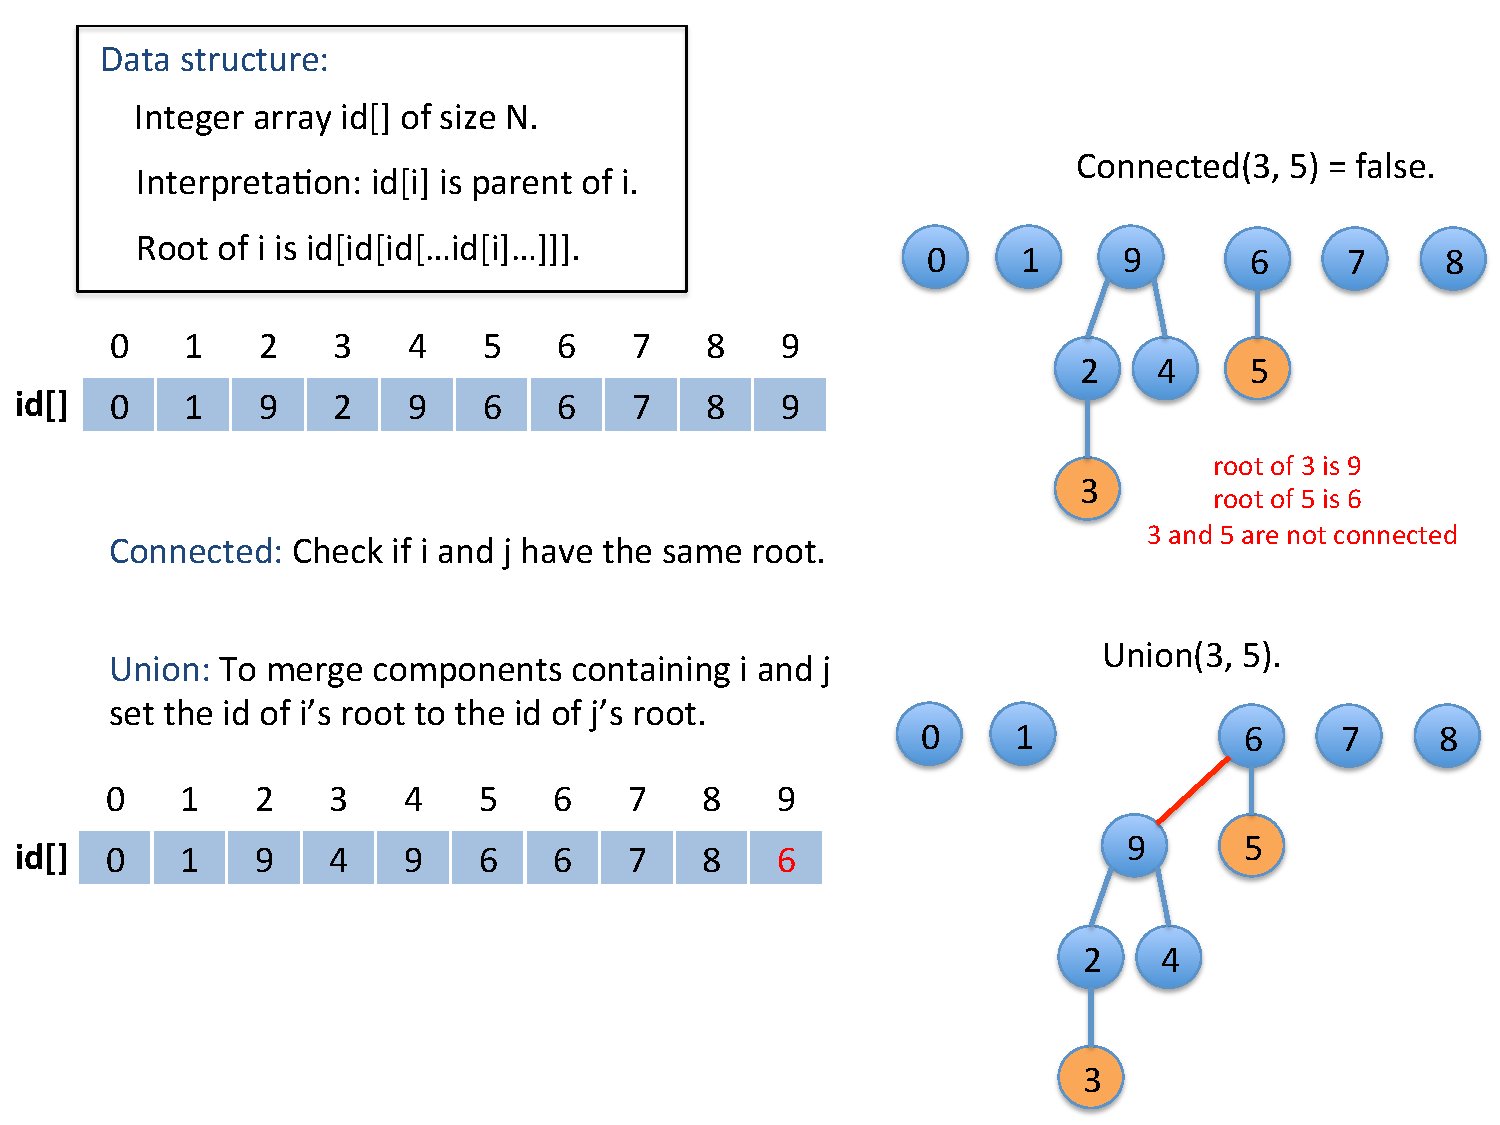
\includegraphics[width=9.5cm]{union_find1.pdf}%
%% \end{center}

\end{frame}

\begin{frame}%[containsverbatim]
\frametitle{Weighted Union Find}

\begin{itemize}
\item Modify \emph{union find} to avoid tall trees.
\item<1-> Keep track of size of each tree (number of nodes).
\item<1-> Balance by linking root of smaller tree to root of larger tree.
\end{itemize}

\begin{overlayarea}{1\textwidth}{0.6\textheight}
\begin{center}
\includegraphics<2>[width=8cm]{union_find27.pdf}%
\includegraphics<3>[width=8cm]{union_find28.pdf}%
\includegraphics<4>[width=8cm]{union_find29.pdf}%
\end{center}
\end{overlayarea}

%% For example:
%% \vspace{-0.5cm}
%% \begin{center}
%% 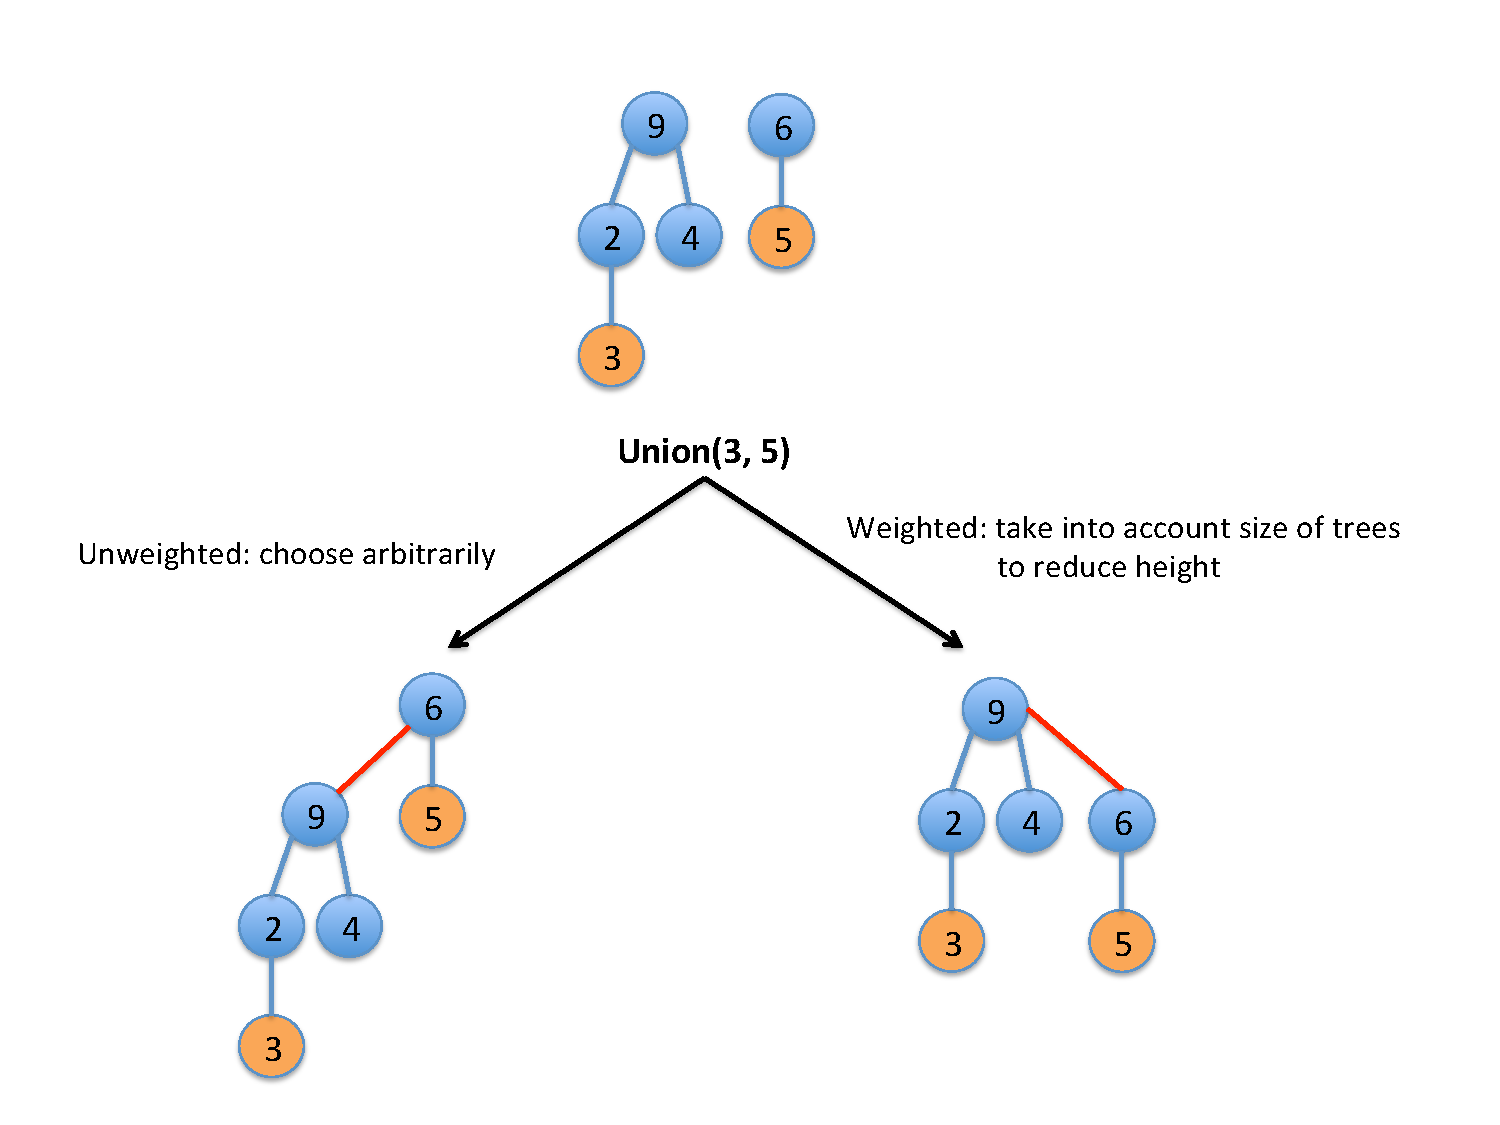
\includegraphics[width=8cm]{union_find2.pdf}%
%% \end{center}

\end{frame}

\begin{frame}%[containsverbatim]
\frametitle{Weighted Union Find Complexity}

\scriptsize

\begin{itemize}
\item \textbf{Find:} takes time proportional to depth of $i$.\\

\vspace{0.1cm}

\item \textbf{Connected:} takes constant time, given roots (uses find to get roots).\\

\vspace{0.1cm}

\item \textbf{Union:} takes constant time, given roots (uses find to get roots).\\

\vspace{0.2cm}
\end{itemize}

\begin{block}<2->{Proposition}
For an array of size $N$, the depth of any node $i$ is at most $\log N$.
\end{block}
\onslide<2->{
\textbf{Proof.} When does depth of $i$ increase?\\
Increases by $1$ when tree $T_1$ containing $i$ is merged into another tree $T_2$. And we have,\\
}
\begin{itemize}
\item<3-> The size of the tree containing $i$ at least doubles since $|T_2| \ge |T_1|$.
\item<4-> The size of tree containing $i$ can double at most $\log N$ times.
\end{itemize}

\begin{overlayarea}{1\textwidth}{0.4\textheight}
\begin{center}
\includegraphics<3->[width=6.5cm]{union_find3.pdf}%
\end{center}
\end{overlayarea}

\end{frame}

\begin{frame}%[containsverbatim]
\frametitle{Weighted Union Find with Path Compression}

\textbf{Quick union with path compression:} just after computing the root of $i$,
set the id of each examined node to point to that root.\\

\begin{center}
\includegraphics<1>[width=10cm]{union_find4.pdf}%
\includegraphics<2>[width=10cm]{union_find5.pdf}%
\includegraphics<3>[width=10cm]{union_find6.pdf}%
\includegraphics<4>[width=10cm]{union_find7.pdf}%
\includegraphics<5>[width=10cm]{union_find8.pdf}%
\includegraphics<6>[width=10cm]{union_find9.pdf}%
\end{center}

\end{frame}

\begin{frame}%[containsverbatim]
\frametitle{Weighted Union Find with Path Compression Complexity}

\scriptsize

\begin{block}<1->{Proposition. [Hopcroft-Ulman, Tarjan]}
Starting from an empty data structure, any sequence of M union-find operations
on $N$ objects makes $\le c ( N + M \log^* N )$ array accesses.
\end{block}
\onslide<2->
Where $\log^*$ is the iterate logarithm function defined by
\[ \log^* x = \left\{
  \begin{array}{l l}
    0 & \quad \text{if $x \le 1$}\\
    1 + \log^*(\log x) & \quad \text{if $x > 1$}
  \end{array} \right.\]
\onslide<3->
\begin{center}
\begin{tabular}{|c|c|}
\hline
$N$ & $\log^* N$\\
\hline
$1$ & $0$\\
$2$ & $1$\\
$4$ & $2$\\
$16$ & $3$\\
$65536$ & $4$\\
$2^{65536}$ & $5$\\
\hline
\end{tabular}
\end{center}

\end{frame}

\begin{frame}[containsverbatim]
\frametitle{Union Find Implementation}

\scriptsize

\begin{lstlisting}[mathescape]
class union_find
{
  vector<int> id; // id[i] = parent of i
  vector<int> sz; // sz[i] = number of objects in subtree rooted at i
  int count;      // number of components
public:
  union_find(int N) : id(N, 0), sz(N, 1)
  {
    count = N;
    for (int i = 0; i < N; i++)
    {
      id[i] = i;
    }
  }
  // ...
\end{lstlisting}

\end{frame}

\begin{frame}[containsverbatim]
\frametitle{Union Find Implementation}

\scriptsize

\begin{lstlisting}[mathescape]
  // ...
  int nb_components()
  {
    return count;
  }

  int size_set(int i)
  {
    return sz[find_set(i)];
  }

  int find_set(int i)
  {
    return (id[i] == i) ? i : (id[i] = find_set(id[i]));
  }
  // ...
\end{lstlisting}

\end{frame}

\begin{frame}[containsverbatim]
\frametitle{Union Find Implementation}

\scriptsize

\begin{lstlisting}[mathescape]
  // ...
  bool connected(int i, int j)
  {
    return find_set(i) == find_set(j);
  }

  void union_set(int p, int q)
  {
    int i = find_set(p);
    int j = find_set(q);
    if (i == j) return;
    // make smaller root point to larger one
    if (sz[i] < sz[j]) { id[i] = j; sz[j] += sz[i]; }
    else               { id[j] = i; sz[i] += sz[j]; }
    --count;
  }
};
\end{lstlisting}

\end{frame}

\begin{frame}[containsverbatim]
\frametitle{\exo}

\footnotesize

\uvalink{11690}{https://uva.onlinejudge.org/index.php?option=com_onlinejudge&Itemid=8&category=24&page=show_problem&problem=2737}\\
\vspace{0.1cm}
or\\
\vspace{0.1cm}
\spojlink{Strange Food Chain}{http://www.spoj.com/problems/CHAIN/}\\
\vspace{0.1cm}
or\\
\vspace{0.1cm}
\uvalink{11987}{https://uva.onlinejudge.org/index.php?option=com_onlinejudge&Itemid=8&category=24&page=show_problem&problem=3138}\\
\vspace{0.4cm}
\hint{
For UVa 11987, you can use the fundamental theorem of software engineering \dSmiley:
\begin{mdframed}[style=exampledefault]
``We can solve any problem by introducing an extra level of indirection.''
\end{mdframed}
}
\end{frame}

\ifanswers

\begin{frame}[containsverbatim]
\frametitle{11690 Solution Implementation}

\scriptsize

\begin{lstlisting}[mathescape]
int main(int argc, char *argv[]) {
  int tc, n, m;
  cin >> tc;
  while (tc--)
  {
    cin >> n >> m;
    int debts[n]{};
    int balance[n]{};
    union_find uf(n);
    for (int i = 0; i < n; ++i)
    {
      cin >> debts[i];
    }
    while (m--)
    {
      int x, y;
      cin >> x >> y;
      uf.union_set(x, y);
    }
    // ...
\end{lstlisting}

\end{frame}

\begin{frame}[containsverbatim]
\frametitle{11690 Solution Implementation}

\scriptsize

\begin{lstlisting}[mathescape]
      // ...
      for (int i = 0; i < n; ++i)
      {
        balance[uf.find_set(i)] += debts[i];
      }

      if (all_of(balance, balance + n, [](int v){ return v == 0; }))
      {
        cout << "POSSIBLE" << endl;
      }
      else cout << "IMPOSSIBLE" << endl;
    }
  return 0;
}
\end{lstlisting}

\end{frame}

\begin{frame}%[containsverbatim]
\frametitle{Strange Food Chain Solution}

\begin{center}
\includegraphics<1>[width=10cm]{strange_food_chain.pdf}%
\includegraphics<2>[width=10cm]{strange_food_chain1.pdf}%
\includegraphics<3>[width=10cm]{strange_food_chain2.pdf}%
\includegraphics<4>[width=10cm]{strange_food_chain3.pdf}%
\includegraphics<5>[width=10cm]{strange_food_chain4.pdf}%
\includegraphics<6>[width=10cm]{strange_food_chain5.pdf}%
\includegraphics<7>[width=10cm]{strange_food_chain6.pdf}%
\end{center}

\end{frame}

\begin{frame}%[containsverbatim]
\frametitle{Strange Food Chain Solution}

\begin{center}
\includegraphics<1>[width=10cm]{strange_food_chain8.pdf}%
\includegraphics<2>[width=10cm]{strange_food_chain9.pdf}%
\includegraphics<3>[width=10cm]{strange_food_chain9bis.pdf}%
\includegraphics<4>[width=10cm]{strange_food_chain10.pdf}%
\includegraphics<5>[width=10cm]{strange_food_chain11.pdf}%
\includegraphics<6>[width=10cm]{strange_food_chain12.pdf}%
\includegraphics<7>[width=10cm]{strange_food_chain13.pdf}%
\includegraphics<8>[width=10cm]{strange_food_chain13_1.pdf}%
\includegraphics<9>[width=10cm]{strange_food_chain13_2.pdf}%
\includegraphics<10>[width=10cm]{strange_food_chain13_3.pdf}%
\includegraphics<11>[width=10cm]{strange_food_chain14.pdf}%
\includegraphics<12>[width=10cm]{strange_food_chain15.pdf}%
\includegraphics<13>[width=10cm]{strange_food_chain16.pdf}%
\includegraphics<14>[width=10cm]{strange_food_chain17.pdf}%
\includegraphics<15>[width=10cm]{strange_food_chain18.pdf}%
%% \includegraphics<16>[width=10cm]{strange_food_chain18_1.pdf}%
%% \includegraphics<17>[width=10cm]{strange_food_chain18_2.pdf}%
%% \includegraphics<18>[width=10cm]{strange_food_chain18_3.pdf}%
%% \includegraphics<19>[width=10cm]{strange_food_chain18_4.pdf}%
\includegraphics<16>[width=10cm]{strange_food_chain19.pdf}%
\includegraphics<17>[width=10cm]{strange_food_chain20.pdf}%
\includegraphics<18>[width=10cm]{strange_food_chain20_1.pdf}%
\includegraphics<19>[width=10cm]{strange_food_chain20_2.pdf}%
\includegraphics<20>[width=10cm]{strange_food_chain20_3.pdf}%
\includegraphics<21>[width=10cm]{strange_food_chain21.pdf}%
\includegraphics<22>[width=10cm]{strange_food_chain22.pdf}%
\includegraphics<23>[width=10cm]{strange_food_chain23.pdf}%
\includegraphics<24>[width=10cm]{strange_food_chain24.pdf}%
\includegraphics<25>[width=10cm]{strange_food_chain25.pdf}%
\includegraphics<26>[width=10cm]{strange_food_chain26.pdf}%
\includegraphics<27>[width=10cm]{strange_food_chain27.pdf}%
\includegraphics<28>[width=10cm]{strange_food_chain28.pdf}%
\includegraphics<29>[width=10cm]{strange_food_chain29.pdf}%
\end{center}

\end{frame}

\begin{frame}[containsverbatim]
\frametitle{Strange Food Chain Solution Implementation}

\scriptsize

\begin{lstlisting}[mathescape]
class union_find
{
  vector<int> id; // id[i] = parent of i
  vector<int> sz; // sz[i] = number of objects in subtree rooted at i
  vector<int> R;  // R(i, id[i])

public:
  union_find(int N) : id(N, 0), sz(N, 1), R(N, 0)
  {
    for (int i = 0; i < N; i++)
    {
      id[i] = i;
    }
  }
  // ...
\end{lstlisting}

\end{frame}

\begin{frame}[containsverbatim]
\frametitle{Strange Food Chain Solution Implementation}

\scriptsize

\begin{lstlisting}[mathescape]
  // ...
  int find_set(int i)
  {
    if (id[i] == i) return i;
    int parent = id[i];
    id[i] = find_set(id[i]);
    R[i] = (R[i] + R[parent] + 3) % 3;
    return id[i];
  }
  bool union_set(int p, int q, int relation)
  {
    int i = find_set(p);
    int j = find_set(q);
    if (i == j) return R[p] == (R[q] + relation) % 3;
    int r = (relation + R[q] - R[p] + 9) % 3;
    if (sz[i] < sz[j]) { id[i] = j; sz[j] += sz[i]; R[i] = r; }
    else               { id[j] = i; sz[i] += sz[j]; R[j] = - r; }
    return true;
  }
};
\end{lstlisting}

\end{frame}

\begin{frame}[containsverbatim]
\frametitle{Strange Food Chain Solution Implementation}

\scriptsize

\begin{lstlisting}[mathescape]
int main(int argc, char *argv[]) {
  int tc;
  cin >> tc;
  while (tc--)
  {
    int N, K;
    cin >> N >> K;
    union_find uf(N + 1);
    int res = 0;
    for (int i = 0; i < K; ++i)
    {
      int D, X, Y;
      cin >> D >> X >> Y;
      if (X > N || Y > N) ++res;
      else if (!uf.union_set(X, Y, D - 1)) ++res;
    }
    cout << res << endl;
  }
  return 0;
}
\end{lstlisting}

\end{frame}

\begin{frame}%[containsverbatim]
\frametitle{11987 Solution}

\begin{center}
\includegraphics<1>[width=10cm]{union_find11987.pdf}%
\includegraphics<2>[width=10cm]{union_find11987_1.pdf}%
\includegraphics<3>[width=10cm]{union_find11987_2.pdf}%
\includegraphics<4>[width=10cm]{union_find11987_2bis.pdf}%
\includegraphics<5>[width=10cm]{union_find11987_3.pdf}%
\includegraphics<6>[width=10cm]{union_find11987_4.pdf}%
\includegraphics<7>[width=10cm]{union_find11987_5.pdf}%
\includegraphics<8>[width=10cm]{union_find11987_6.pdf}%
\includegraphics<9>[width=10cm]{union_find11987_7.pdf}%
\end{center}

\end{frame}


\begin{frame}[containsverbatim]
\frametitle{11987 Solution Implementation}

\scriptsize

\begin{lstlisting}[mathescape]
class union_find {
  vector<int> id;   // id[i]= parent of i
  vector<int> sz;   // sz[i]= number of objects in subtree rooted at i
  vector<long> sum; // sum[i]= sum of elements in subtree rooted at i
  int count;        // number of components
  int N;

public:
  union_find(int N) : id(2 * N + 1, 0), sz(N + 1, 1), sum(N + 1, 0)
  {
    this->N = N;
    count = N;
    for (int i = 1; i <= N; i++)
    {
      id[i] = id[N + i] = N + i;
      sum[i] = i;
    }
  }
  // ...
\end{lstlisting}

\end{frame}

\begin{frame}[containsverbatim]
\frametitle{11987 Solution Implementation}

\scriptsize

\begin{lstlisting}[mathescape]
  // ...
  int find_set(int i)
  {
    return (id[i] == i) ? i : (id[i] = find_set(id[i]));
  }

  int size_set(int i)
  {
    return sz[find_set(i) - N];
  }

  int sum_set(int i)
  {
    return sum[find_set(i) - N];
  }
  // ...
\end{lstlisting}

\end{frame}

\begin{frame}[containsverbatim]
\frametitle{11987 Solution Implementation}

\scriptsize

\begin{lstlisting}[mathescape]
  // ...
  void union_set(int p, int q)
  {
    int i = find_set(p);
    int j = find_set(q);
    if (i == j) return;
    // make smaller root point to larger one
    if (sz[i - N] < sz[j - N])
    {
      id[i] = j; sz[j - N] += sz[i - N];
      sum[j - N] += sum[i - N];
    }
    else
    {
      id[j] = i; sz[i - N] += sz[j - N];
      sum[i - N] += sum[j - N];
    }
    count--;
  }
  // ...
\end{lstlisting}

\end{frame}

\begin{frame}[containsverbatim]
\frametitle{11987 Solution Implementation}

\scriptsize

\begin{lstlisting}[mathescape]
  // ...
  void move(int p, int q)
  {
    int i = find_set(p);
    int j = find_set(q);

    if (i == j) return;

    id[p] = j;

    sum[j - N] += p;
    sz[j - N]++;

    sum[i - N] -= p;
    sz[i - N]--;
  }
};
\end{lstlisting}

\end{frame}

\begin{frame}[containsverbatim]
\frametitle{11987 Solution Implementation}

\scriptsize

\begin{lstlisting}[mathescape]
int main(int argc, char *argv[]) {
  int N, M;
  while (cin >> N >> M)
  {
    union_find uf(N);
    while (M--)
    {
      int command, p, q;
      cin >> command;
      if (command == 1) { cin >> p >> q; uf.union_set(p, q); }
      else if (command == 2) { cin >> p >> q; uf.move(p, q); }
      else
      {
        cin >> p;
        cout << uf.size_set(p) << " " << uf.sum_set(p) << endl;
      }
    }
  }
  return 0;
}
\end{lstlisting}

\end{frame}

\fi

% StSpanningTree Codeforces

\subsection{Heap}

\begin{frame}%[containsverbatim]
\frametitle{Heap}

A \textbf{heap} is a tree-based data structure, that contains \textbf{keys}
(each \texttt{key} can be associated with a \textbf{value}),
based on the heap order property:
\vspace{0.4cm}
\begin{block}<1->{Heap order}
For every node $i$,  \texttt{key}$(i) \ge$ \texttt{key}$($\texttt{parent}$(i))$.
\end{block}
\vspace{0.3cm}

\end{frame}

\begin{frame}[containsverbatim]
\frametitle{Heap Example}

\begin{center}
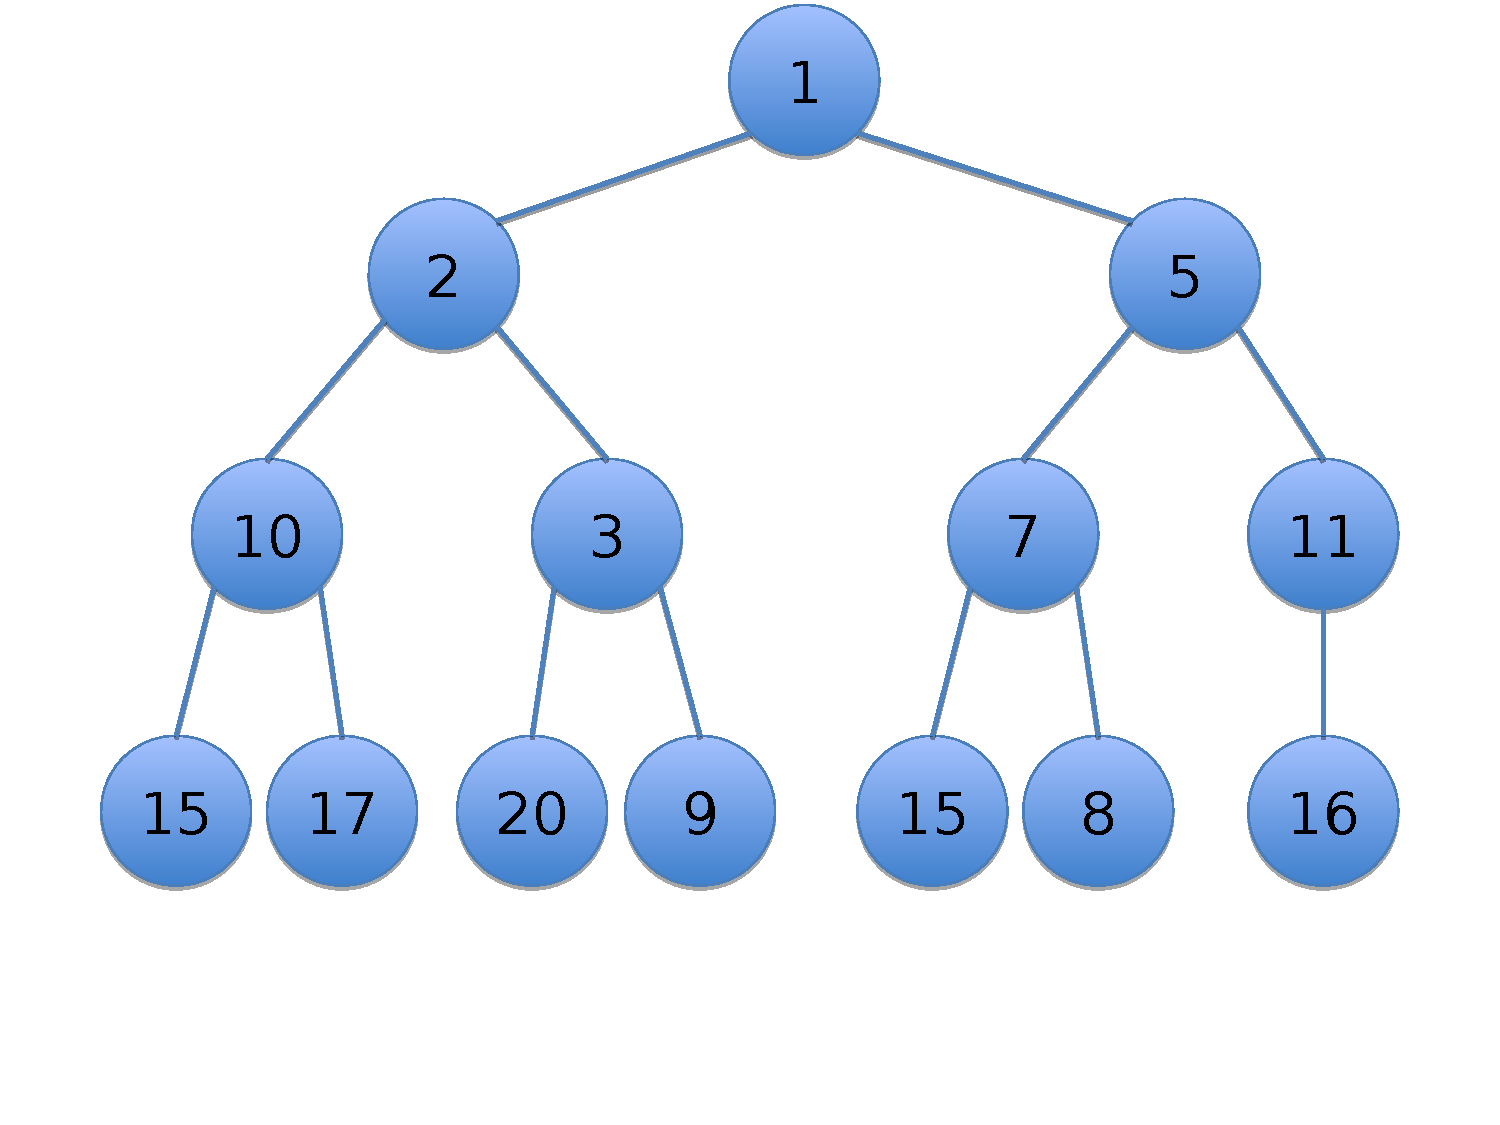
\includegraphics[width=10cm]{heap.pdf}%
\end{center}

\end{frame}

\begin{frame}%[containsverbatim]
\frametitle{Heap Implementation}

\begin{itemize}
\item We suppose that there will be no more than $N$ elements in the heap.
\vspace{0.1cm}
\item<2-> We can use an array $H$ of size $(N+1)$ to represent the heap.
\vspace{0.1cm}
\item<3-> The heap nodes correspond to the positions in this array.
\vspace{0.1cm}
\item<4-> $H[1]$ is the root.
\vspace{0.1cm}
\item<5-> If there is $n$ elements in the heap, they are in position $1$ to $n$.
\vspace{0.1cm}
\item<6-> For any node at position $i$, the children are the nodes at positions
\begin{itemize}
\item \texttt{leftChild(i) = 2i}.
\item \texttt{rightChild(i) = 2i + 1}.
\end{itemize}
\vspace{0.1cm}
\item<7-> The parent is at position
\begin{itemize}
\item \texttt{parent(i) = } $\lfloor i/2 \rfloor$.
\end{itemize}

\end{itemize}

\end{frame}

\begin{frame}[containsverbatim]
\frametitle{Heap Implementation Example}

\begin{center}
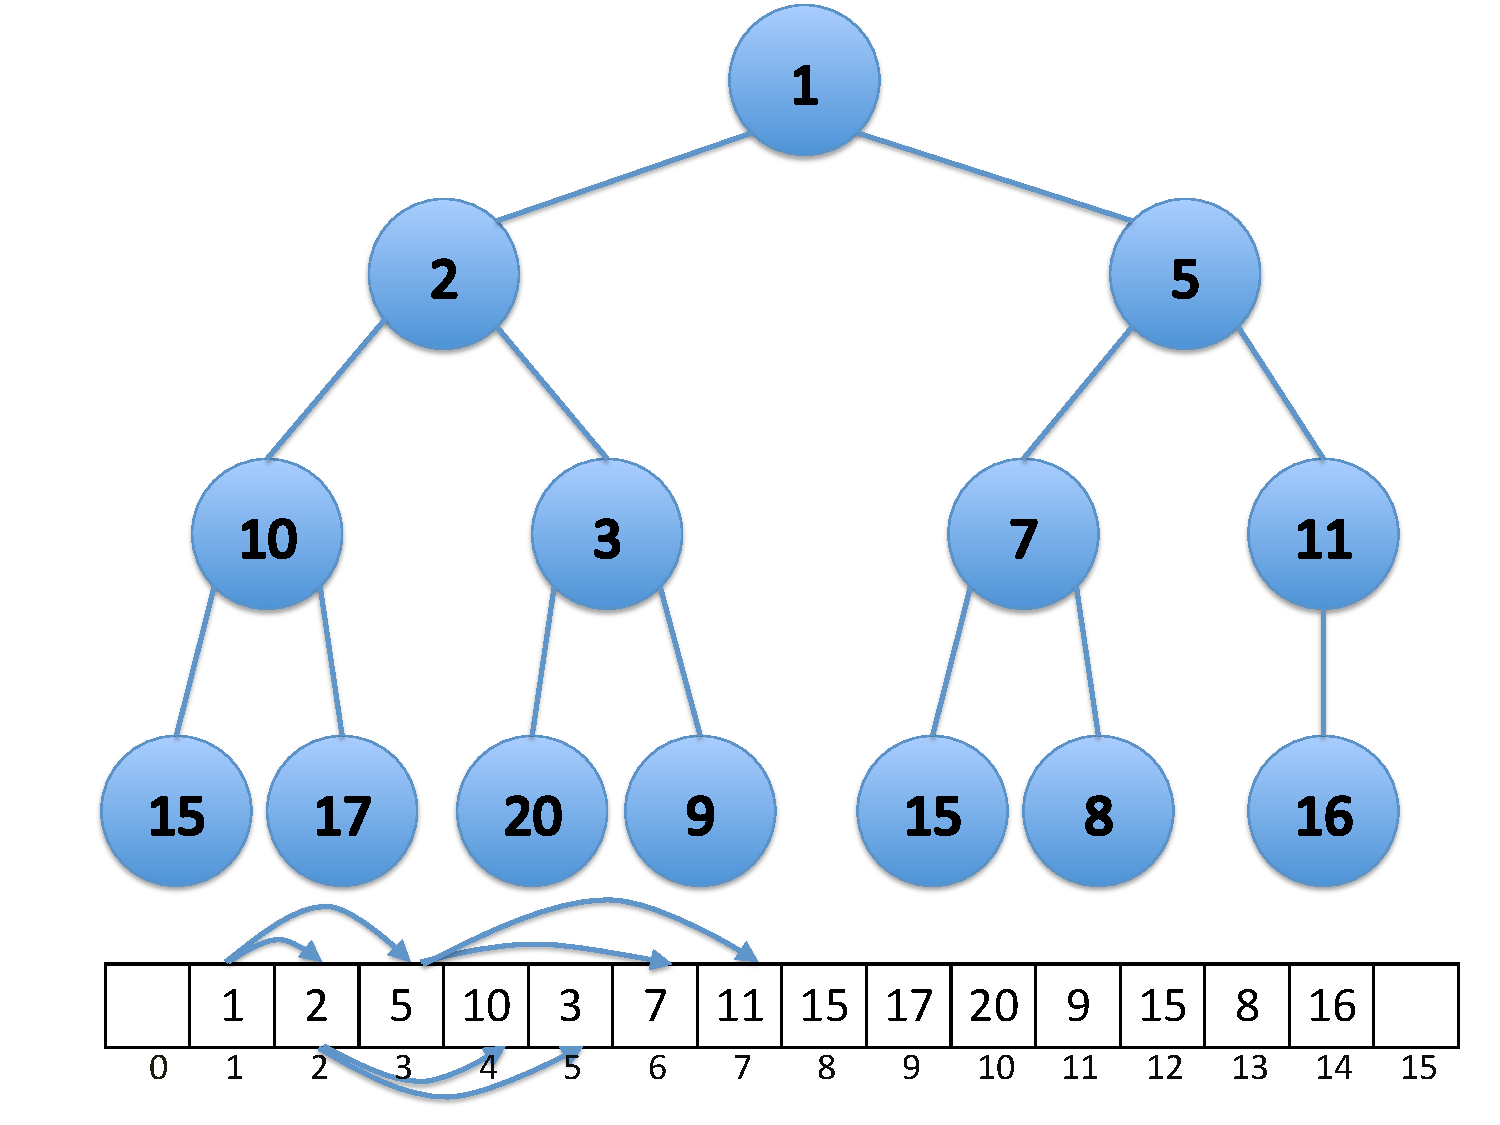
\includegraphics[width=9cm]{heap_implementation.pdf}%
\end{center}

\end{frame}

\begin{frame}%[containsverbatim]
\frametitle{Heap Operations}

An heap has, at least, the following operations:
\vspace{0.3cm}
\begin{itemize}

\item<1-> \textbf{insert(H, v)}: Insert item \texttt{v} (a key or key/value pair) into the heap \texttt{H}.

\vspace{0.3cm}

\item<2-> \textbf{findMin(H)}: Return the minimum item of the heap \texttt{H} but does not remove it.

\vspace{0.3cm}

\item<3-> \textbf{deleteMin(H)}: Remove the minimum item of the heap \texttt{H}.
\end{itemize}

\end{frame}

\begin{frame}[containsverbatim]
\frametitle{Heap Operation: Insert}

\begin{center}
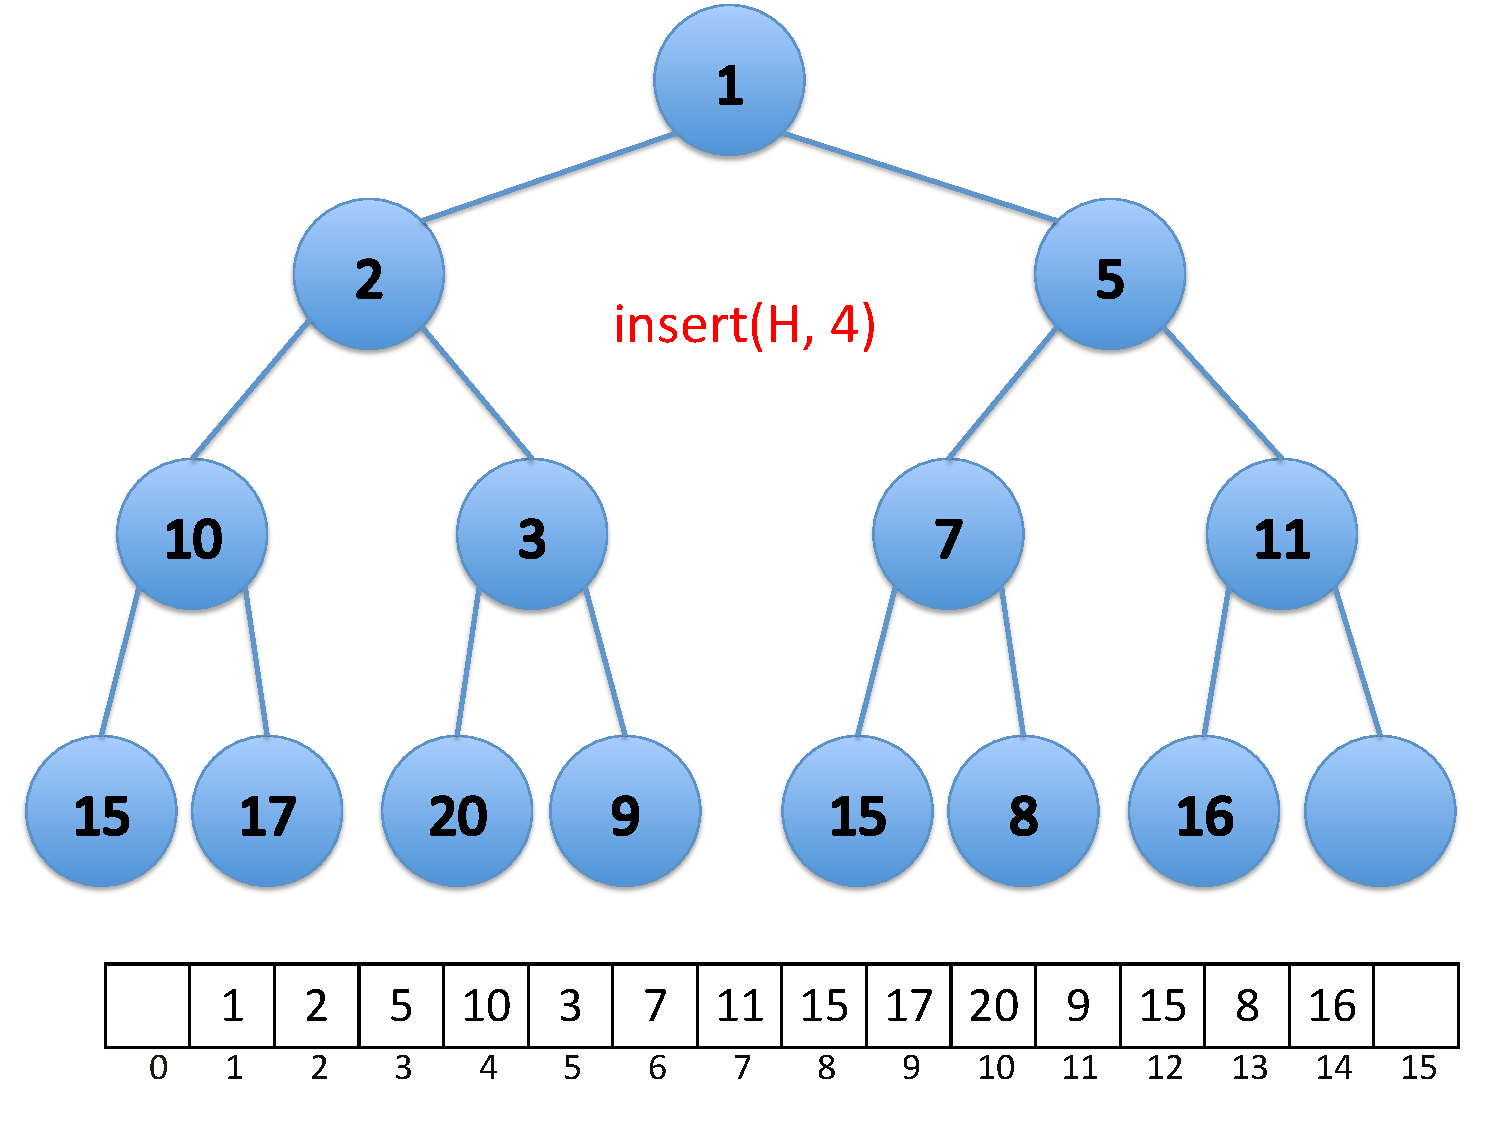
\includegraphics[width=9cm]{heap_insert1.pdf}%
\end{center}

\end{frame}

\begin{frame}[containsverbatim]
\frametitle{Heap Operation: Insert}

\begin{center}
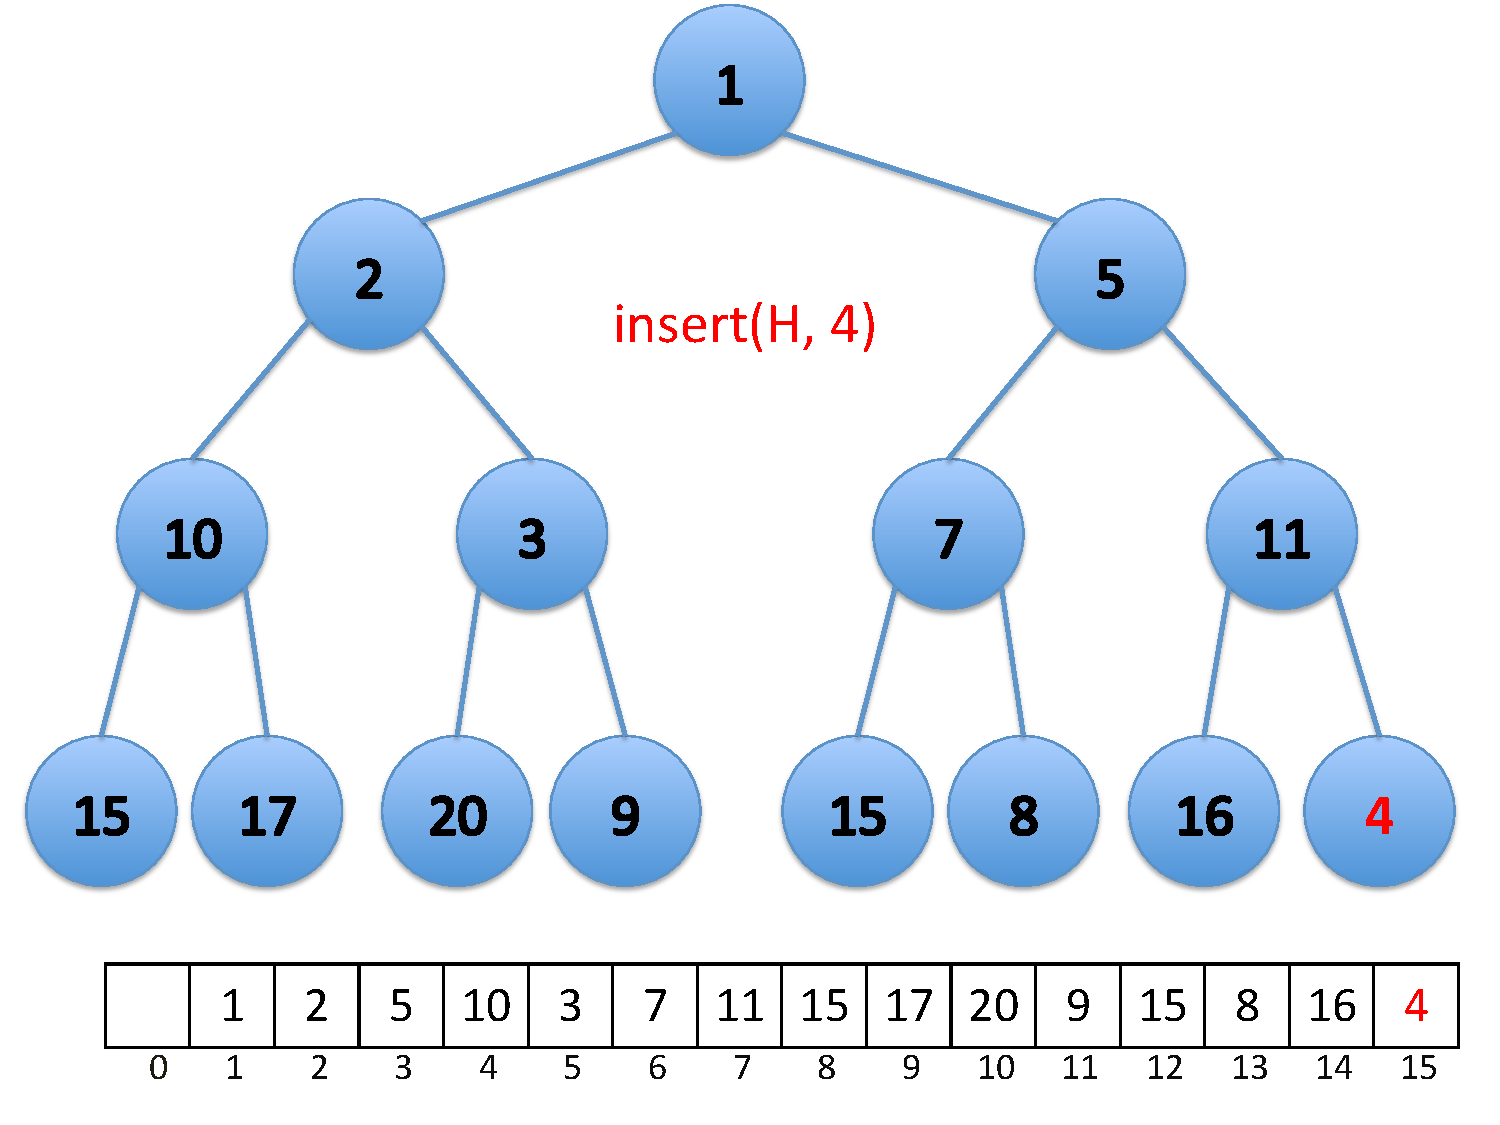
\includegraphics[width=9cm]{heap_insert2.pdf}%
\end{center}

\end{frame}

\begin{frame}[containsverbatim]
\frametitle{Heap Operation: Insert}

\begin{center}
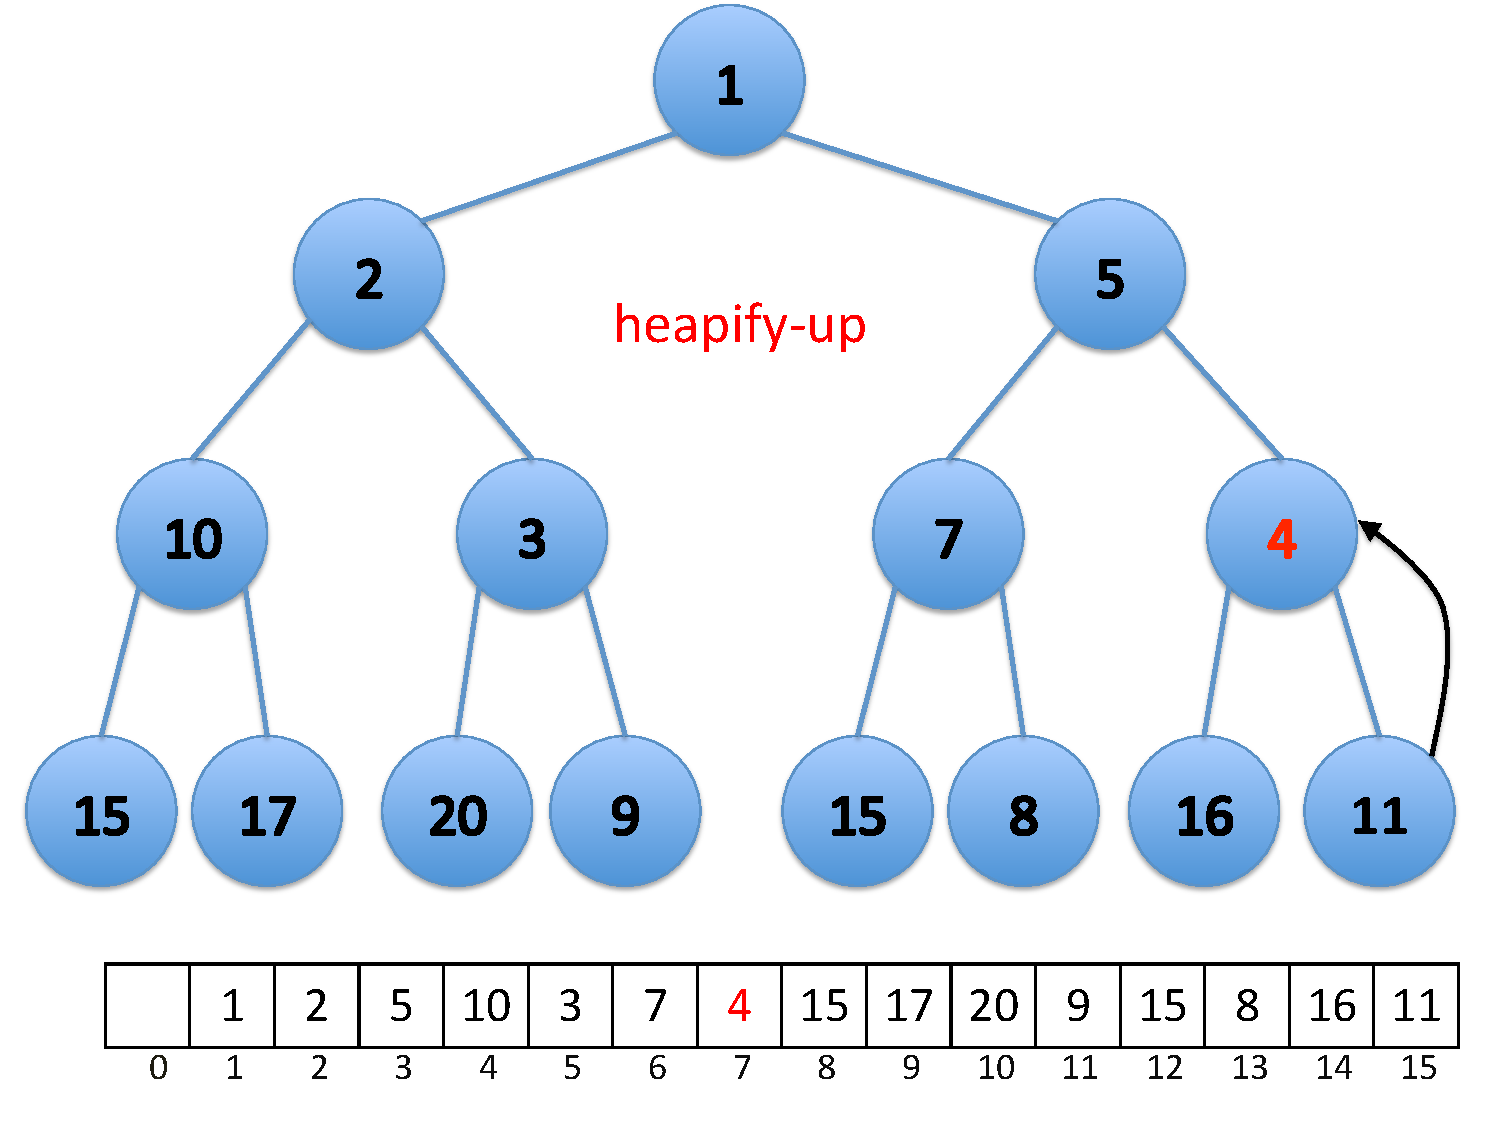
\includegraphics[width=9cm]{heap_insert3.pdf}%
\end{center}

\end{frame}

\begin{frame}[containsverbatim]
\frametitle{Heap Operation: Insert}

\begin{center}
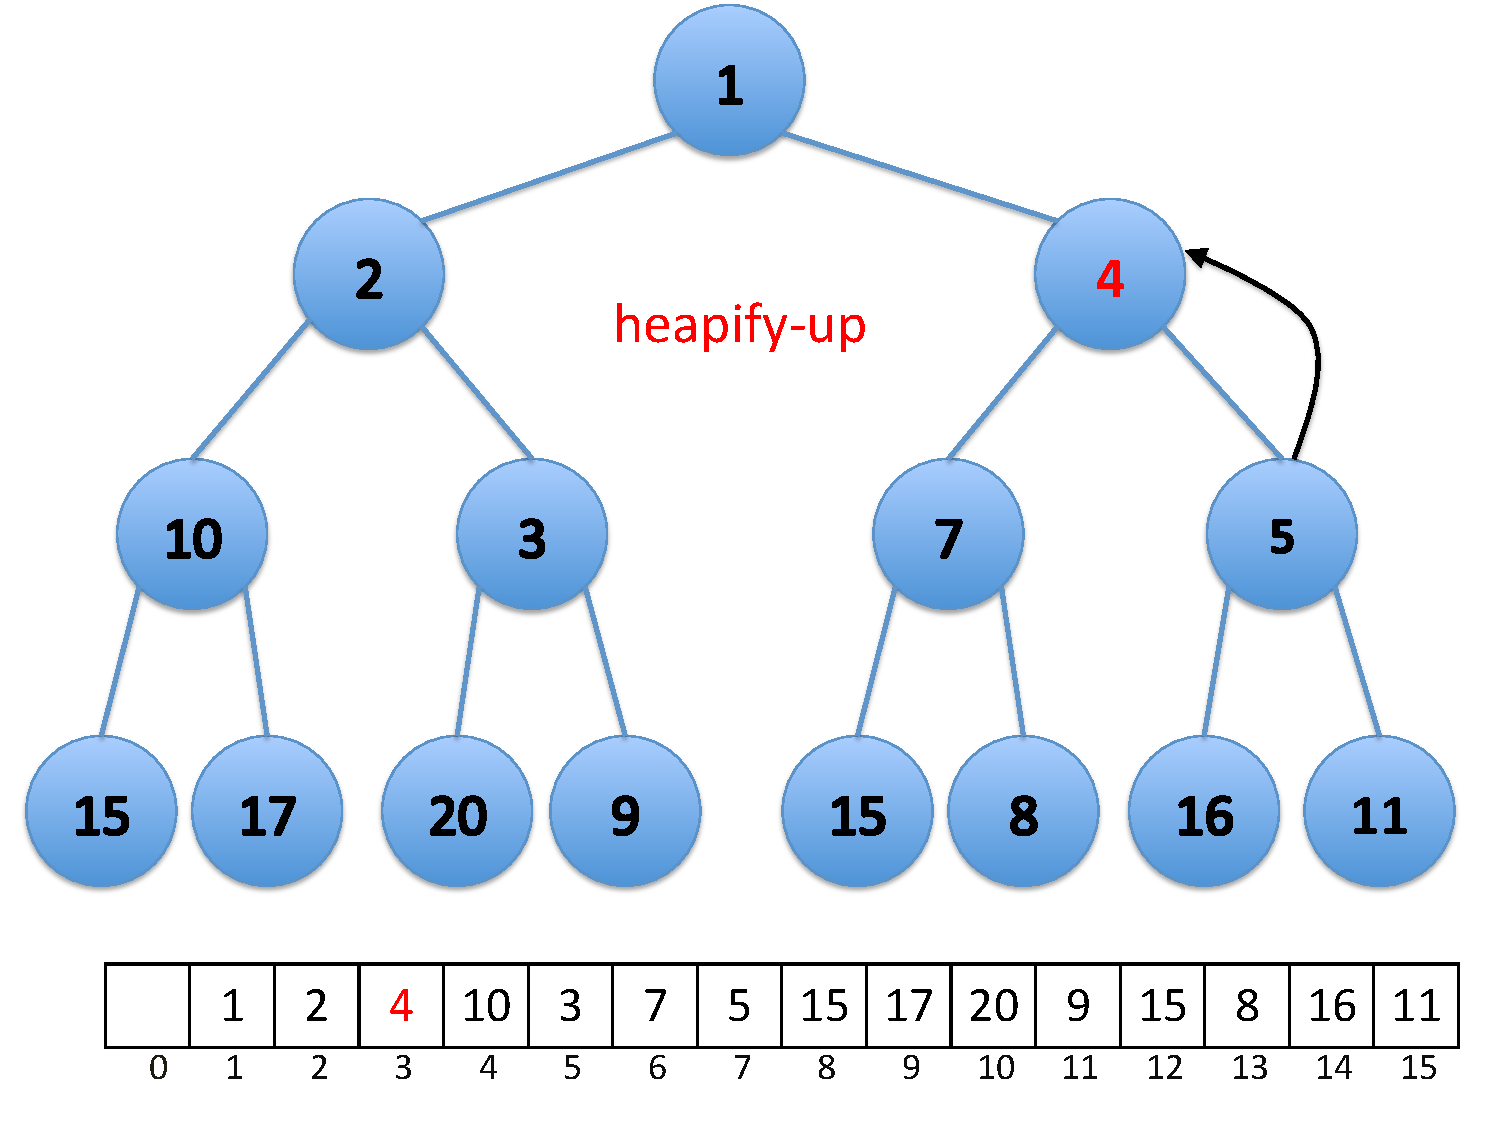
\includegraphics[width=9cm]{heap_insert4.pdf}%
\end{center}

\end{frame}

\begin{frame}[containsverbatim]
\frametitle{Heap Operation: FindMin}

\begin{center}
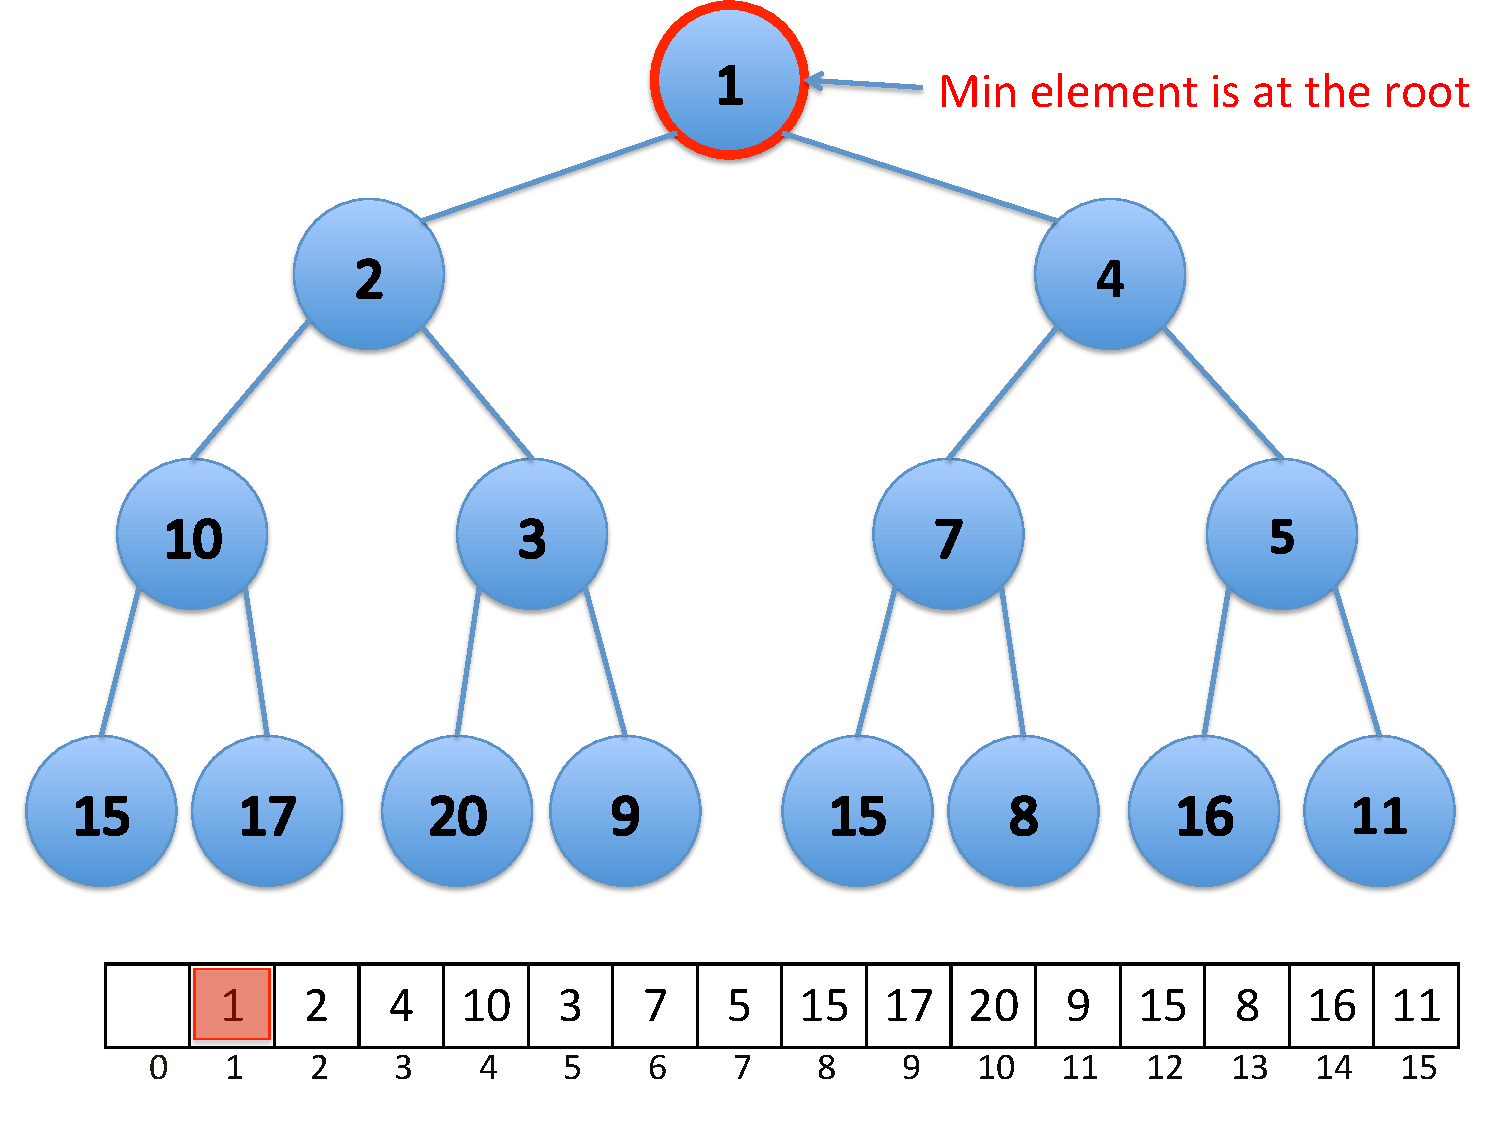
\includegraphics[width=9cm]{heap_find_min.pdf}%
\end{center}

\end{frame}

\begin{frame}[containsverbatim]
\frametitle{Heap Operation: DeleteMin}

\begin{center}
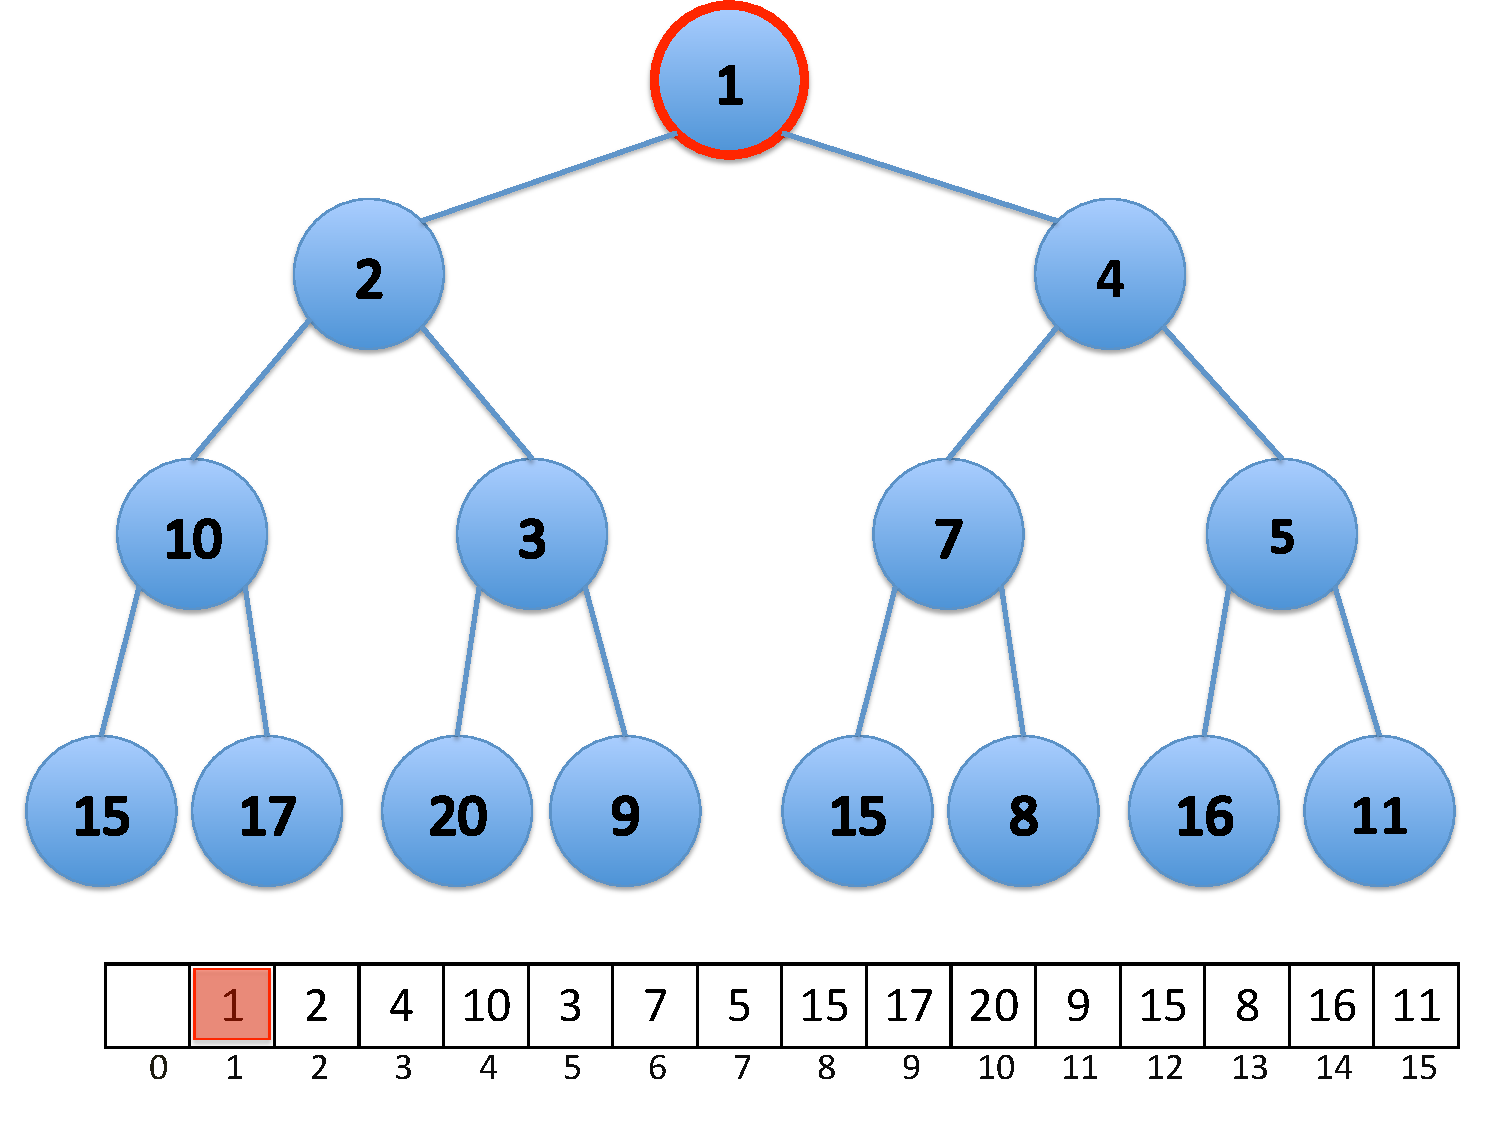
\includegraphics[width=9cm]{heap_delete_min1.pdf}%
\end{center}

\end{frame}

\begin{frame}[containsverbatim]
\frametitle{Heap Operation: DeleteMin}

\begin{center}
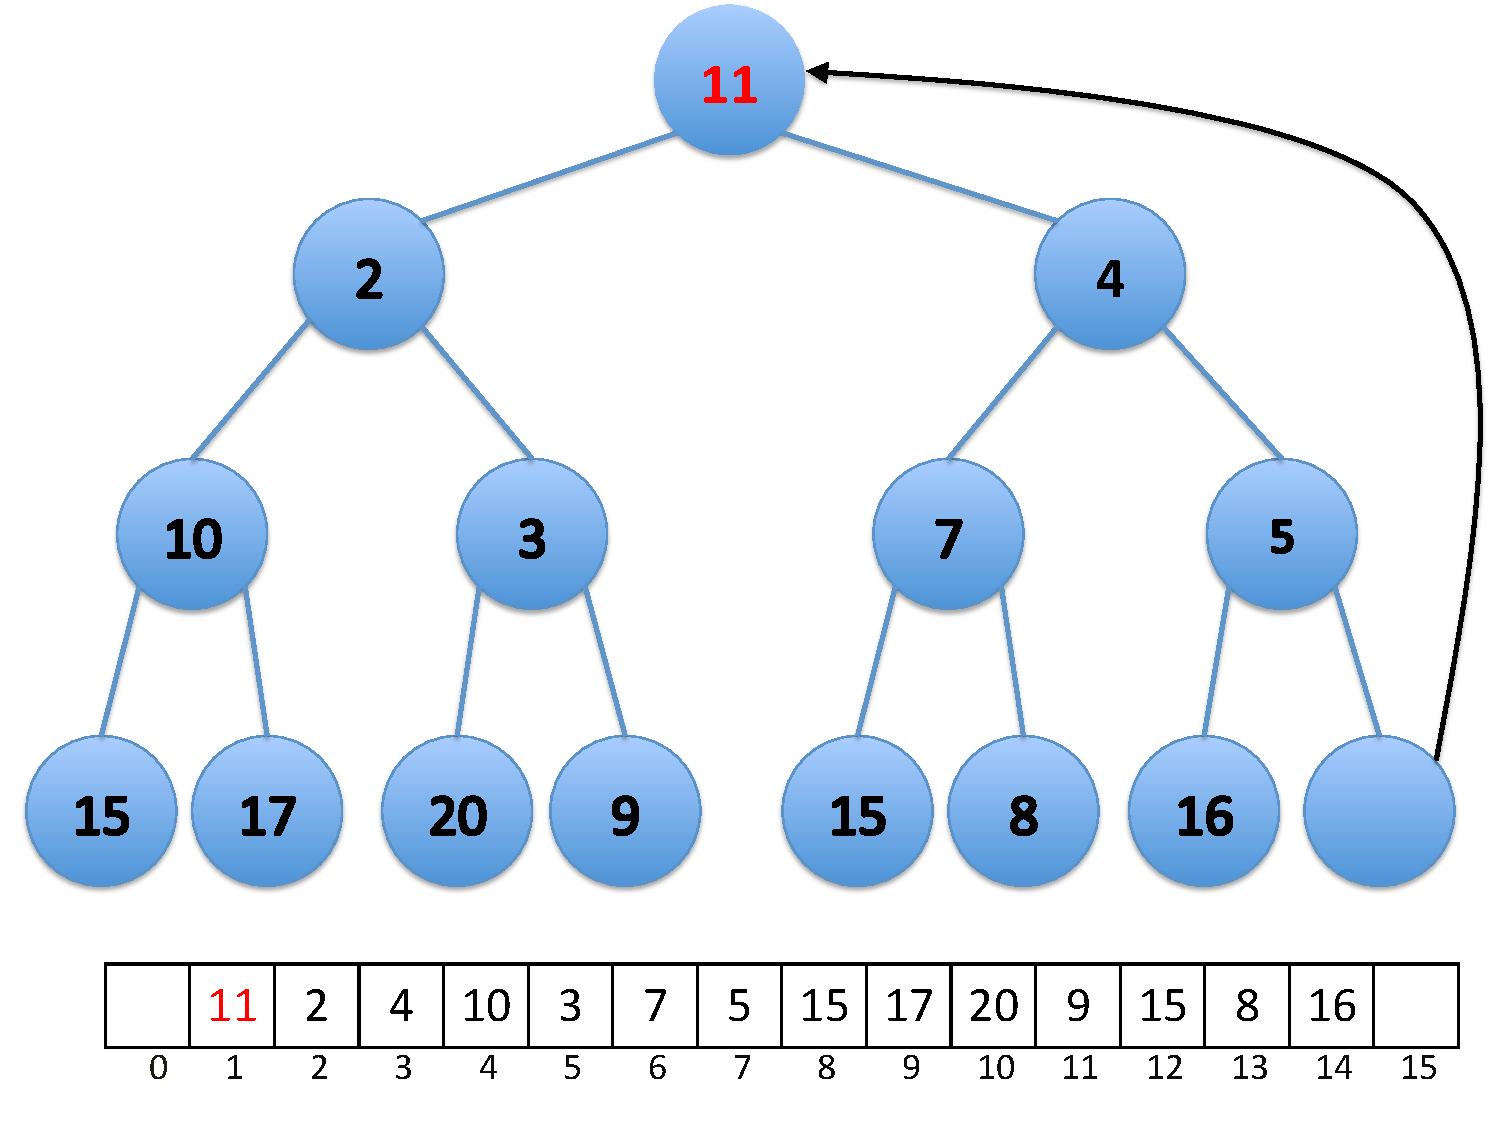
\includegraphics[width=9cm]{heap_delete_min2.pdf}%
\end{center}

\end{frame}

\begin{frame}[containsverbatim]
\frametitle{Heap Operation: DeleteMin}

\begin{center}
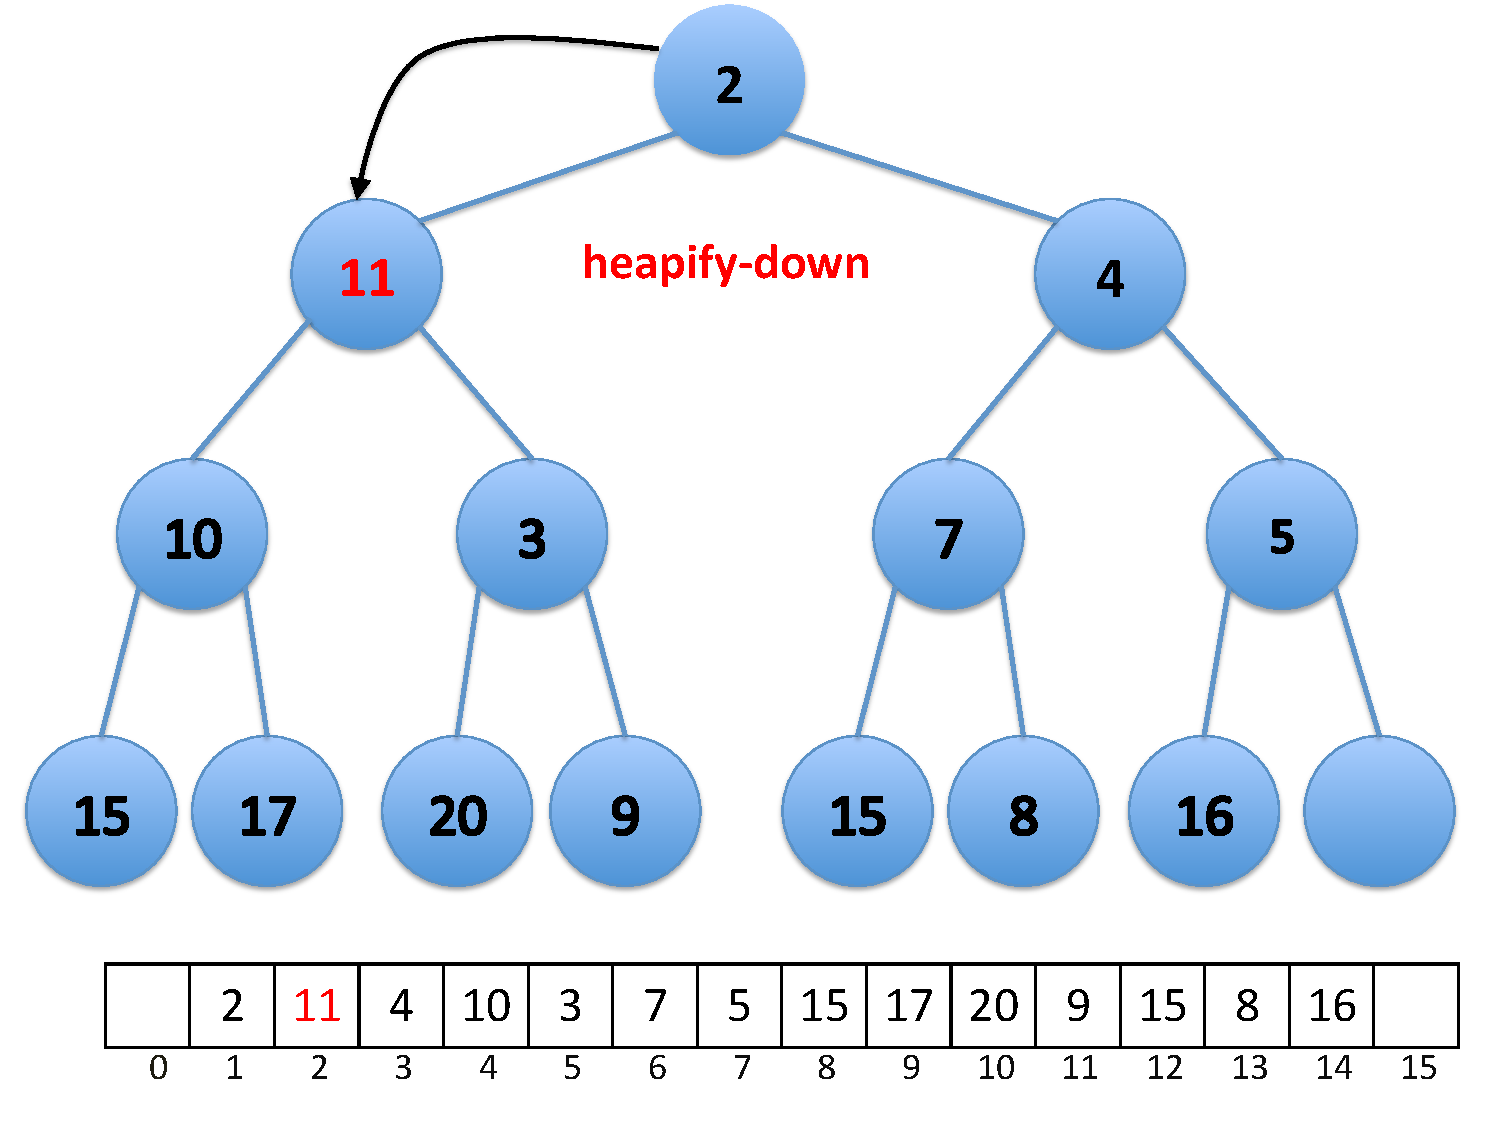
\includegraphics[width=9cm]{heap_delete_min3.pdf}%
\end{center}

\end{frame}

\begin{frame}[containsverbatim]
\frametitle{Heap Operation: DeleteMin}

\begin{center}
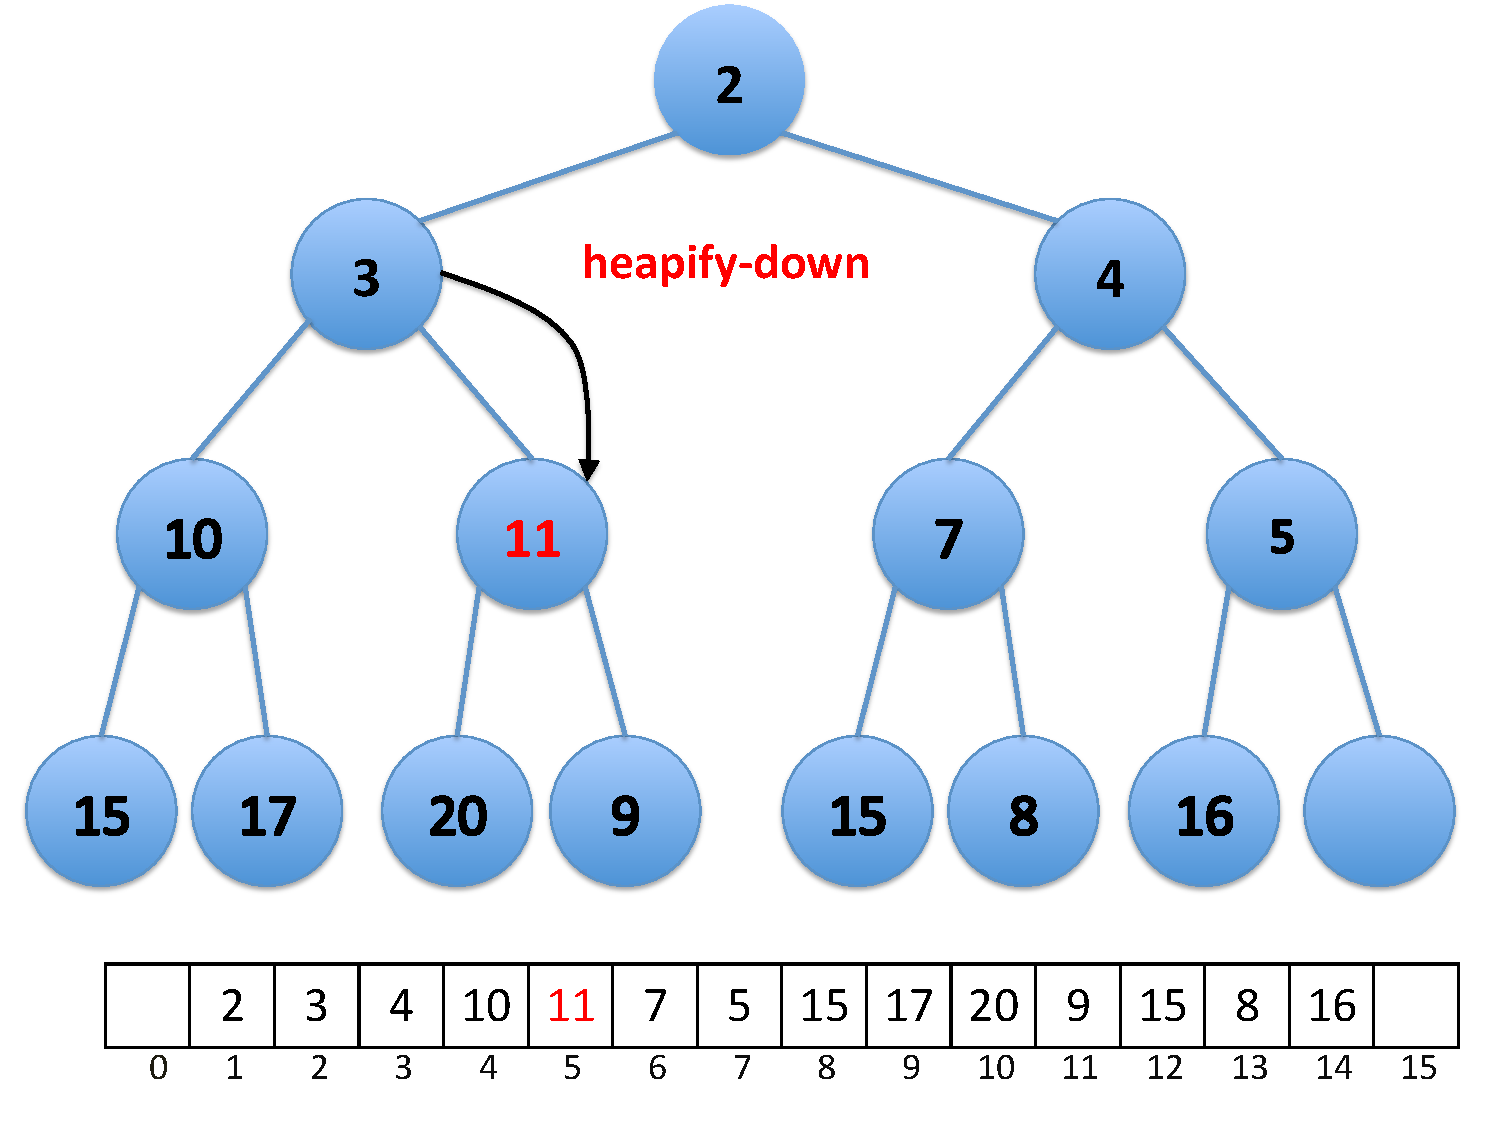
\includegraphics[width=9cm]{heap_delete_min4.pdf}%
\end{center}

\end{frame}

\begin{frame}[containsverbatim]
\frametitle{Heap Operation: DeleteMin}

\begin{center}
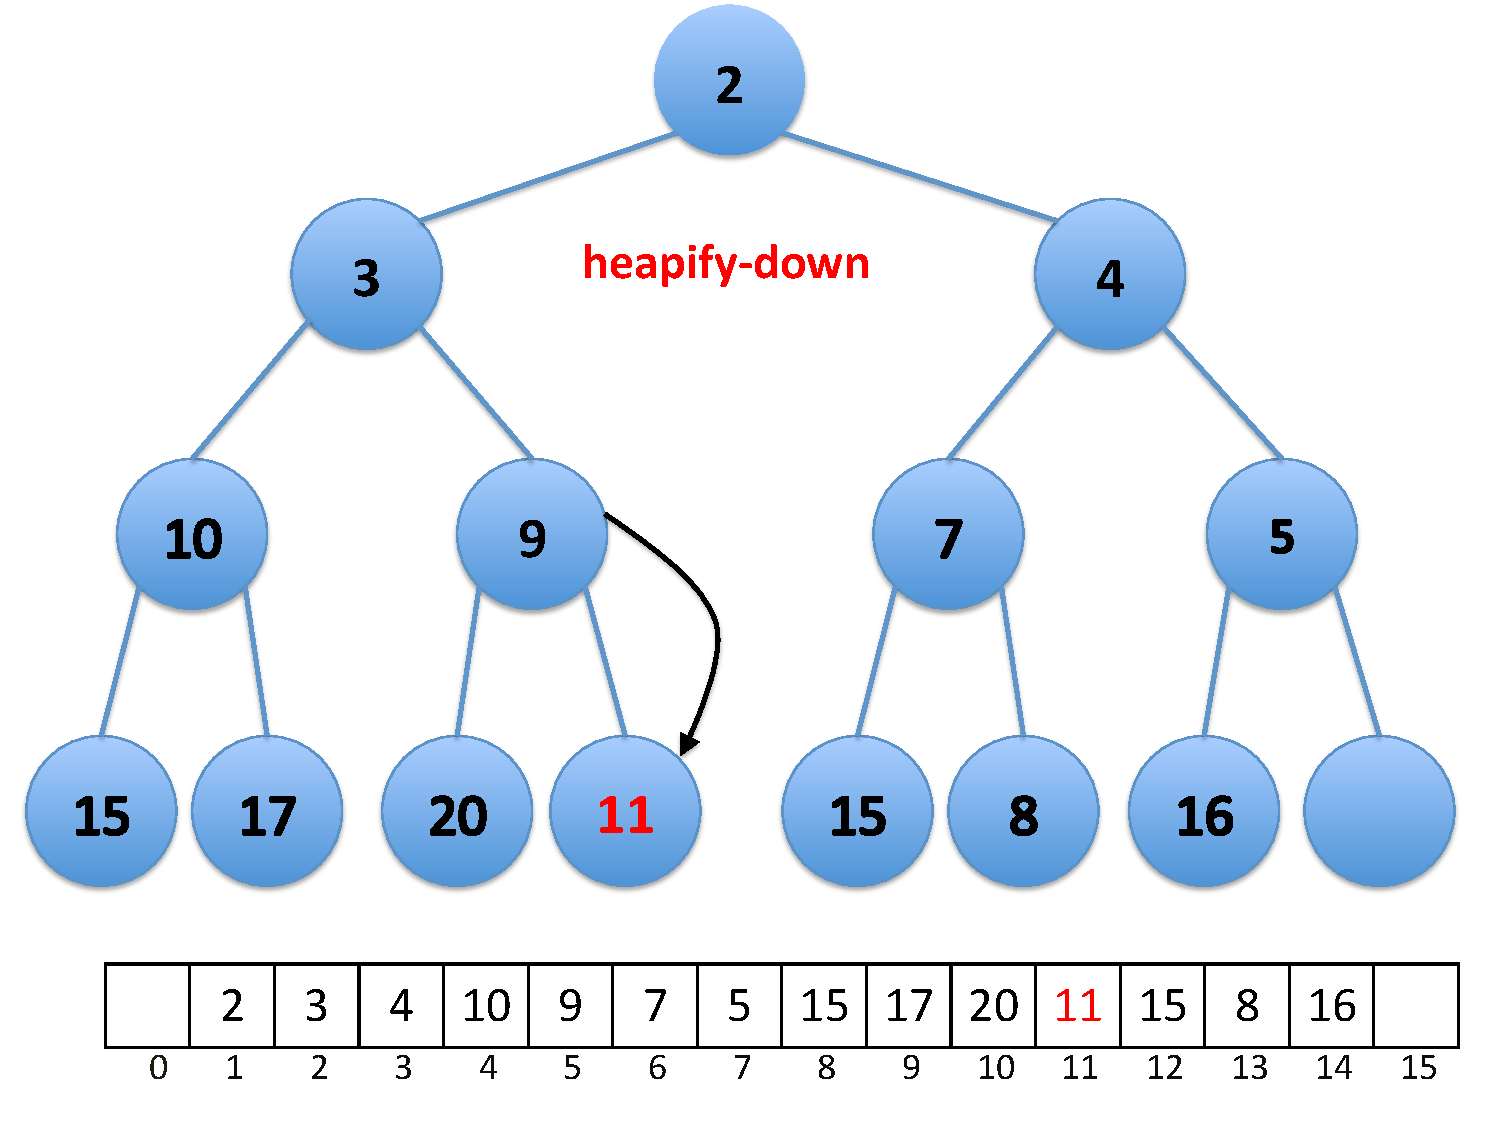
\includegraphics[width=9cm]{heap_delete_min5.pdf}%
\end{center}

\end{frame}

\begin{frame}%[containsverbatim]
\frametitle{Heap Operations Complexity}

\begin{itemize}

\item \textbf{insert(H, v)}: $O(\log n)$.
\vspace{0.6cm}

\item \textbf{findMin(H)}: $O(1)$.
\vspace{0.6cm}

\item \textbf{deleteMin(H)}: $O(\log n)$.

\end{itemize}

\end{frame}

\begin{frame}%[containsverbatim]
\frametitle{Priority Queue}

%\footnotesize

\begin{itemize}
\item The \textbf{heap} previously defined can be used to create a \textbf{priority queue}.\\

\vspace{0.2cm}

\item<2-> The class \textbf{priority\_queue} implements a queue from which elements are read according to their
priority.

%\vspace{0.1cm}

\begin{itemize}
%\footnotesize
\item<2-> \textbf{push()} inserts an element into the queue.

\vspace{0.18cm}

\item<2-> \textbf{top()} and \textbf{pop()} access and remove the next element.

\vspace{0.18cm}

\item<2-> The next element is the element that has the highest priority.

\vspace{0.18cm}

\item<2-> By default, the highest priority is determined using \lstinline{operator <}.

%% \begin{itemize}
%% \footnotesize

%% \vspace{0.1cm}

%% \item<6-> Elements are partially sorted according to their value. By default, the elements are sorted by using \texttt{operator <} in \textbf{descending order}.

%% \vspace{0.2cm}

%% \item<7-> The next element is always the``highest'' element. If more than
%% one ``highest'' element exists, which element comes next is undefined.

%% \end{itemize}

\end{itemize}

\end{itemize}

\end{frame}

\begin{frame}[containsverbatim]
\frametitle{Priority Queue Example}

\scriptsize

\begin{lstlisting}[mathescape]
int main(int argc, char *argv[]) {
  priority_queue<int> q1;
  q1.push(5);
  q1.push(2);
  q1.push(42);
  cout << q1.top() << ' ';
  q1.pop();
  cout << q1.top() << endl;
  priority_queue<int, vector<int>, greater<int>> q2;
  q2.push(5);
  q2.push(2);
  q2.push(42);
  cout << q2.top() << ' ';
  q2.pop();
  cout << q2.top() << endl;
  return 0;
}
\end{lstlisting}

\begin{verbatim}
42 5
2 5
\end{verbatim}

\end{frame}

\begin{frame}[containsverbatim]
\frametitle{\exo}

\uvalink{10107}{https://uva.onlinejudge.org/index.php?option=com_onlinejudge&Itemid=8&category=24&page=show_problem&problem=1048}\\
\vspace{0.2cm}
or\\
\vspace{0.2cm}
\uvalink{11134}{https://uva.onlinejudge.org/index.php?option=com_onlinejudge&Itemid=8&category=24&page=show_problem&problem=2075}

\end{frame}

\ifanswers

\begin{frame}%[containsverbatim]
\frametitle{10107 Solution}

\begin{center}
\includegraphics<1>[width=10cm]{uva10107.pdf}%
\includegraphics<2>[width=10cm]{uva10107_1.pdf}%
\includegraphics<3>[width=10cm]{uva10107_3.pdf}%
\includegraphics<4>[width=10cm]{uva10107_2_2.pdf}%
\includegraphics<5>[width=10cm]{uva10107_4.pdf}%
\includegraphics<6>[width=10cm]{uva10107_5.pdf}%
\includegraphics<7>[width=10cm]{uva10107_6.pdf}%
\includegraphics<8>[width=10cm]{uva10107_7.pdf}%
\includegraphics<9>[width=10cm]{uva10107_8.pdf}%
\includegraphics<10>[width=10cm]{uva10107_9.pdf}%
\includegraphics<11>[width=10cm]{uva10107_10.pdf}%
\includegraphics<12>[width=10cm]{uva10107_11.pdf}%
\includegraphics<13>[width=10cm]{uva10107_12.pdf}%
\includegraphics<14>[width=10cm]{uva10107_13.pdf}%
\includegraphics<15>[width=10cm]{uva10107_14.pdf}%
\includegraphics<16>[width=10cm]{uva10107_15.pdf}%
\includegraphics<17>[width=10cm]{uva10107_16.pdf}%
\includegraphics<18>[width=10cm]{uva10107_17.pdf}%
\includegraphics<19>[width=10cm]{uva10107_18.pdf}%
\includegraphics<20>[width=10cm]{uva10107_19.pdf}%
\includegraphics<21>[width=10cm]{uva10107_20.pdf}%
\includegraphics<22>[width=10cm]{uva10107_21.pdf}%
\includegraphics<23>[width=10cm]{uva10107_22.pdf}%
\end{center}

\end{frame}

\begin{frame}[containsverbatim]
\frametitle{10107 Implementation}
\scriptsize
\begin{lstlisting}
int main(int argc, char *argv[]) {
  priority_queue<long> left_max_pq;
  priority_queue<long, vector<long>, greater<long>> right_min_pq;
  int X;
  left_max_pq.push(numeric_limits<long>::min());
  right_min_pq.push(numeric_limits<long>::max());
  while (cin >> X)
  {
    long left = left_max_pq.top(), right = right_min_pq.top();
    if (left_max_pq.size() <= right_min_pq.size())
    {
      if (X <= right) left_max_pq.push(X);
      else
      {
        left_max_pq.push(right_min_pq.top());
        right_min_pq.pop();
        right_min_pq.push(X);
      }
    }
    // ...
\end{lstlisting}

\end{frame}

\begin{frame}[containsverbatim]
\frametitle{10107 Implementation}
\scriptsize
\begin{lstlisting}
     // ...
     else // left_max_pq.size() > right_min_pq.size()
     {
       if (X >= left) right_min_pq.push(X);
       else {
         right_min_pq.push(left_max_pq.top());
         left_max_pq.pop();
         left_max_pq.push(X);
       }
     }
     if (right_min_pq.size() == left_max_pq.size())
       cout << (right_min_pq.top() + left_max_pq.top()) / 2 << endl;
     else
     {
       if (right_min_pq.size() < left_max_pq.size())
         cout << left_max_pq.top() << endl;
       else cout << right_min_pq.top() << endl;
     }
  }
}
\end{lstlisting}

\end{frame}

\begin{frame}%[containsverbatim]
\frametitle{11134 Solution}

\begin{center}
\includegraphics<1>[width=7cm]{uva11134.pdf}%
\includegraphics<2>[width=7cm]{uva11134_1.pdf}%
\includegraphics<3>[width=7cm]{uva11134_2.pdf}%
\includegraphics<4>[width=7cm]{uva11134_3.pdf}%
\includegraphics<5>[width=7cm]{uva11134_4.pdf}%
\includegraphics<6>[width=7cm]{uva11134_5.pdf}%
\includegraphics<7>[width=7cm]{uva11134_6.pdf}%
\includegraphics<8>[width=7cm]{uva11134_7.pdf}%
\includegraphics<9>[width=7cm]{uva11134_8.pdf}%
\includegraphics<10>[width=7cm]{uva11134_9.pdf}%
\includegraphics<11>[width=7cm]{uva11134_10.pdf}%
\includegraphics<12>[width=7cm]{uva11134_11.pdf}%
\includegraphics<13>[width=7cm]{uva11134_12.pdf}%
\includegraphics<14>[width=7cm]{uva11134_13.pdf}%
\includegraphics<15>[width=7cm]{uva11134_14.pdf}%
\includegraphics<16>[width=7cm]{uva11134_15.pdf}%
\includegraphics<17>[width=7cm]{uva11134_16.pdf}%
\includegraphics<18>[width=7cm]{uva11134_17.pdf}%
\includegraphics<19>[width=7cm]{uva11134_18.pdf}%
\includegraphics<20>[width=7cm]{uva11134_19.pdf}%
%\includegraphics<21>[width=7cm]{uva11134_20.pdf}%
\includegraphics<21>[width=7cm]{uva11134_21.pdf}%
\includegraphics<22>[width=7cm]{uva11134_22.pdf}%
\includegraphics<23>[width=7cm]{uva11134_23.pdf}%
\includegraphics<24>[width=7cm]{uva11134_24.pdf}%
\includegraphics<25>[width=7cm]{uva11134_25.pdf}%
\includegraphics<26>[width=7cm]{uva11134_26.pdf}%
\includegraphics<27>[width=7cm]{uva11134_27.pdf}%
\includegraphics<28>[width=7cm]{uva11134_28.pdf}%
\end{center}

\end{frame}

\begin{frame}[containsverbatim]
\frametitle{11134 Implementation}
\scriptsize
\begin{lstlisting}
struct range {
  int left, right, id;
  bool operator<(const range& range) const {
    return right > range.right;
  }
};
bool solve(const vector<vector<range>>& ranges, vector<int>& coord) {
  int N = ranges.size();
  priority_queue<range> pq;
  for (int i = 1; i < N; ++i) {
    for_each(ranges[i].begin(), ranges[i].end(),
            [&pq](const range& r){ pq.push(r); });
    if (pq.size() == 0) return false;
    range r = pq.top();
    pq.pop();
    if (r.right < i) return false;
    coord[r.id] = i;
  }
  return true;
}
\end{lstlisting}

\end{frame}

\begin{frame}[containsverbatim]
\frametitle{11134 Implementation}
\scriptsize
\begin{lstlisting}
int main(int argc, char *argv[])
{
  int N;
  while (cin >> N && N)
  {
    range x;
    range y;
    vector<vector<range>> xrange(N + 1, vector<range>());
    vector<vector<range>> yrange(N + 1, vector<range>());
    for (int i = 0; i < N; ++i)
    {
      cin >> x.left >> y.left >> x.right >> y.right;
      x.id = i;
      y.id = i;
      xrange[x.left].push_back(x);
      yrange[y.left].push_back(y);
    }
    // ...
\end{lstlisting}

\end{frame}

\begin{frame}[containsverbatim]
\frametitle{11134 Implementation}
\scriptsize
\begin{lstlisting}
    // ...
    vector<int> rook_x(N + 1, 0);
    vector<int> rook_y(N + 1, 0);
    bool possible = solve(xrange, rook_x) && solve(yrange, rook_y);
    if (possible)
    {
      for (int i = 0; i < N; ++i)
      {
        cout << rook_x[i] << " " << rook_y[i] << endl;
      }
    }
    else cout << "IMPOSSIBLE" << endl;
  }
  return 0;
}
\end{lstlisting}

\end{frame}

\fi

%% \subsection{Binary Search Tree}

%% % Dynamic Inversion UVA

%% \begin{frame}%[containsverbatim]
%% \frametitle{Binary Search Tree}

%% \scriptsize

%% \begin{block}{Binary Search Tree}
%% A Binary Search Tree is a binary tree in symmetric order.
%% \end{block}

%% \onslide<2->
%% \begin{block}{Binary Tree}
%% A binary tree is either
%% \begin{itemize}
%% \item Empty.
%% \item A node with a left and a right tree.
%% \end{itemize}
%% \end{block}

%% \onslide<3->
%% \begin{block}{Symmetric order}
%% Each node has a key, and every node's key is
%% \begin{itemize}
%% \item Larger than all keys in its left subtree.
%% \item Smaller than all keys in its right subtree.
%% \end{itemize}
%% \end{block}

%% \end{frame}

%% \begin{frame}[containsverbatim]
%% \frametitle{Binary Search Tree Example}

%% \begin{center}
%% 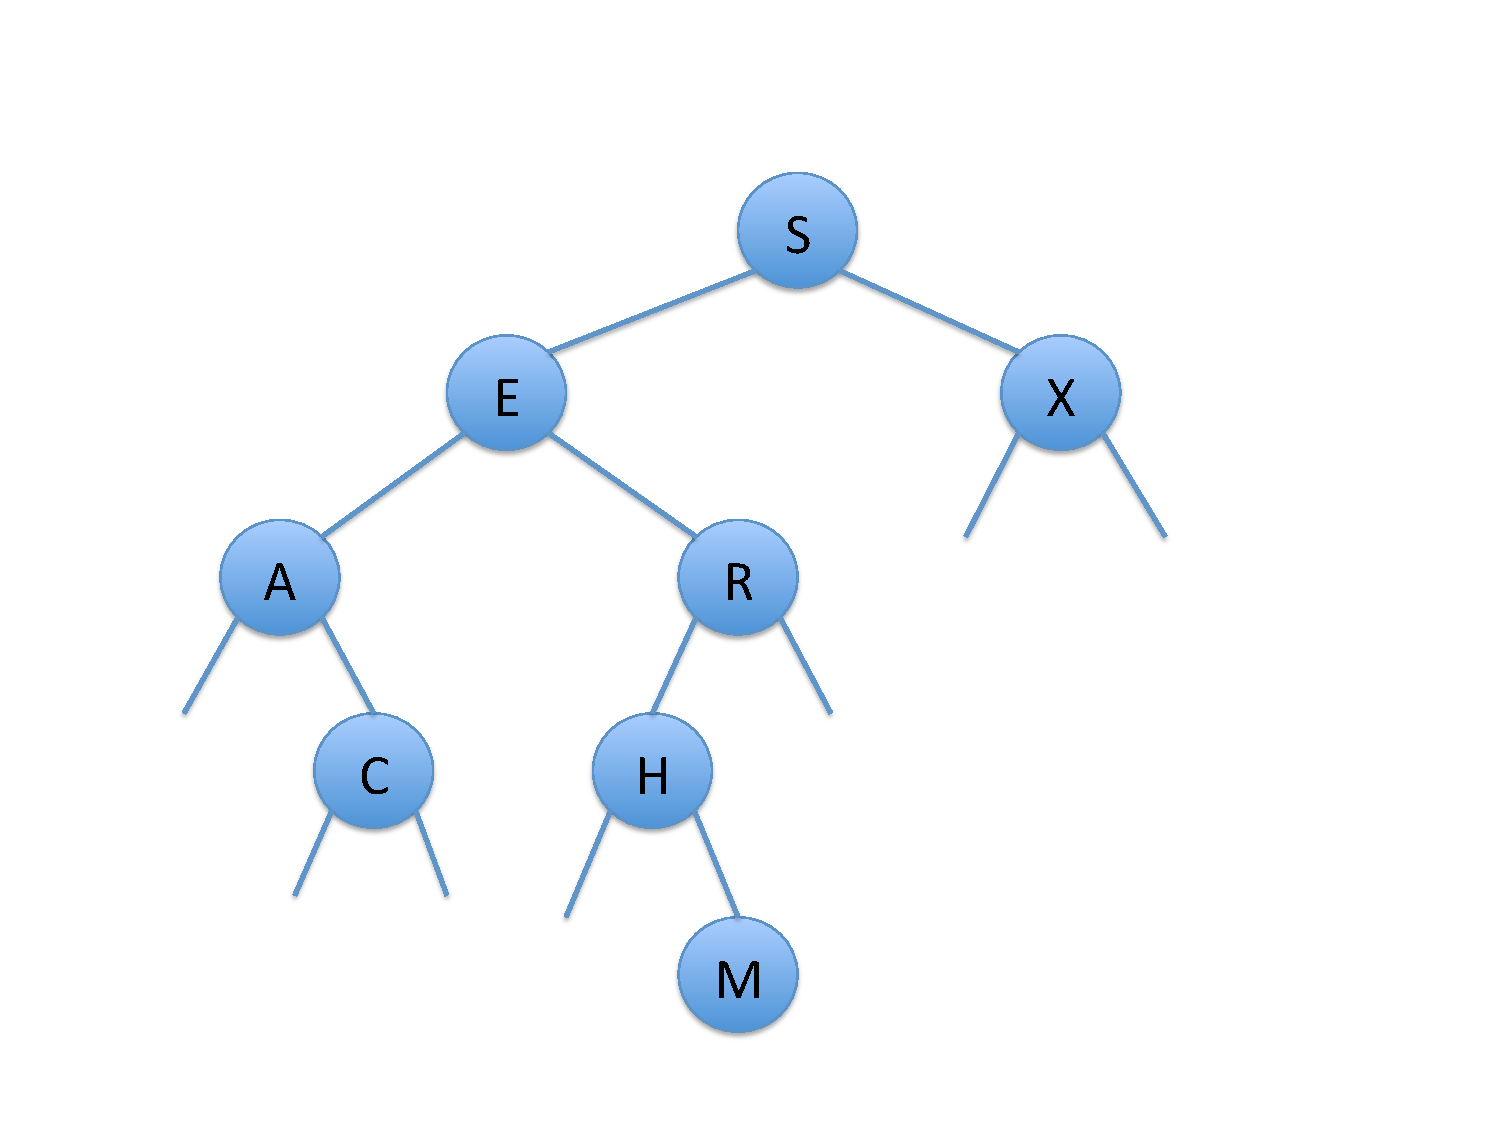
\includegraphics[width=10cm]{binary_search_tree.pdf}%
%% \end{center}

%% \end{frame}

%% \begin{frame}[containsverbatim]
%% \frametitle{Binary Search Tree: Find}

%% \begin{center}
%% 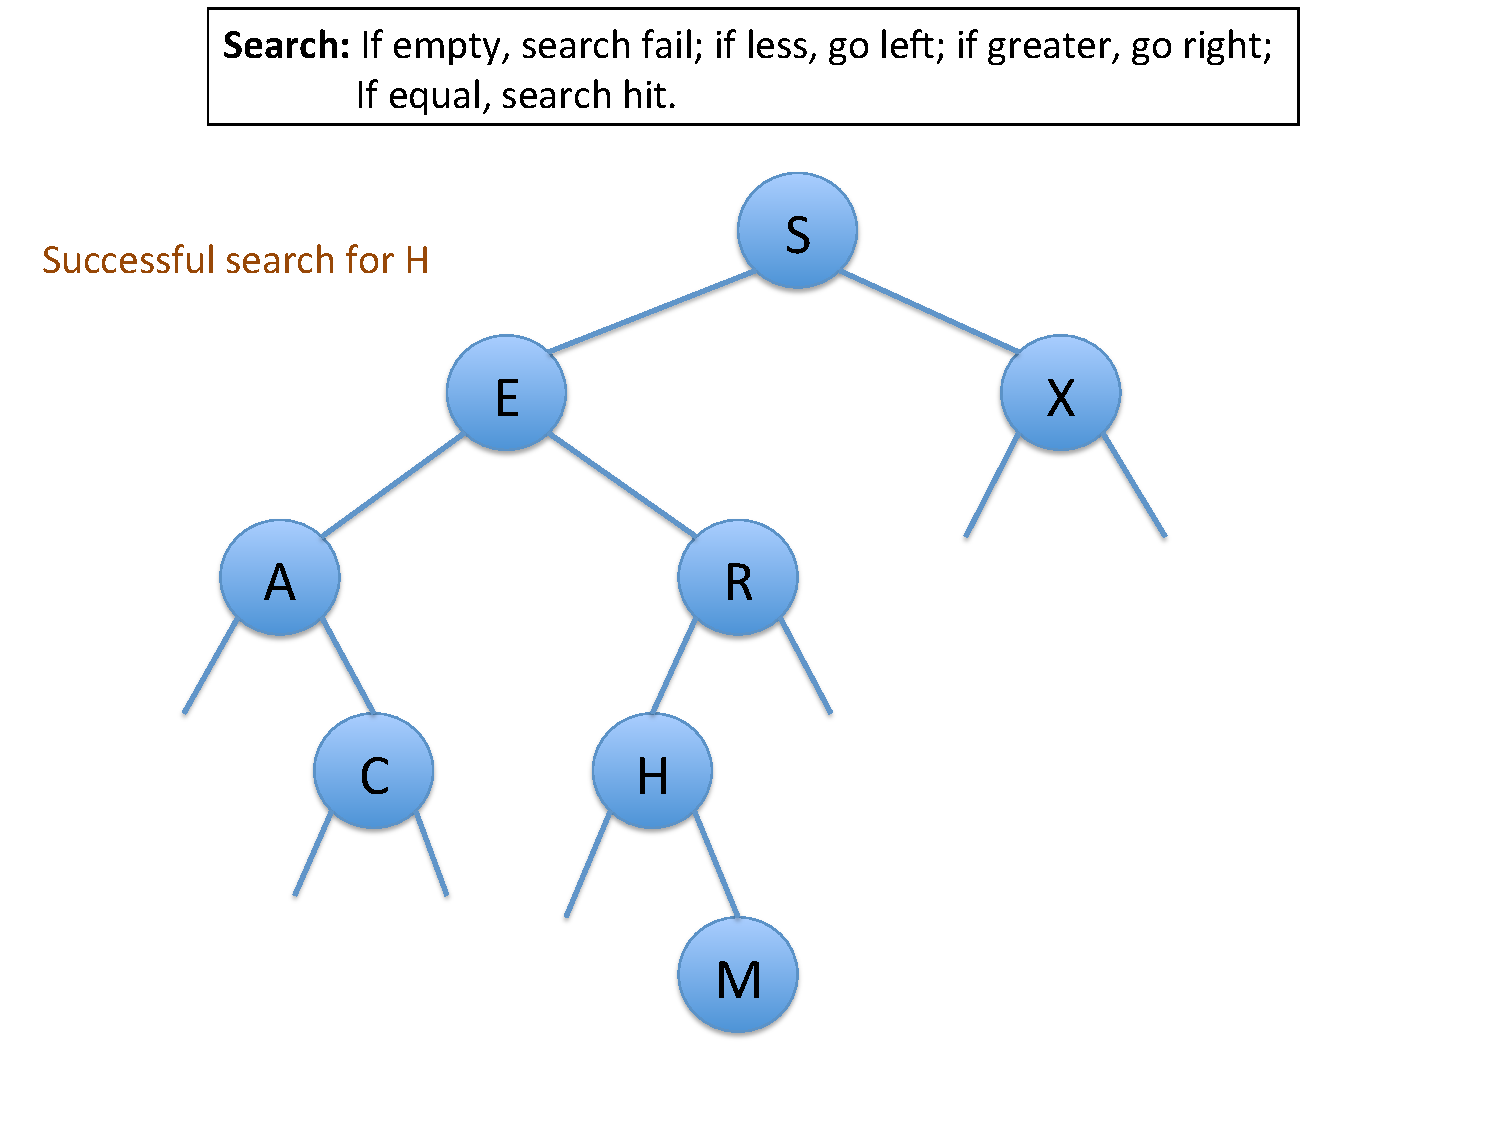
\includegraphics[width=10cm]{binary_search_tree_find1.pdf}%
%% \end{center}

%% \end{frame}

%% \begin{frame}[containsverbatim]
%% \frametitle{Binary Search Tree: Find}

%% \begin{center}
%% 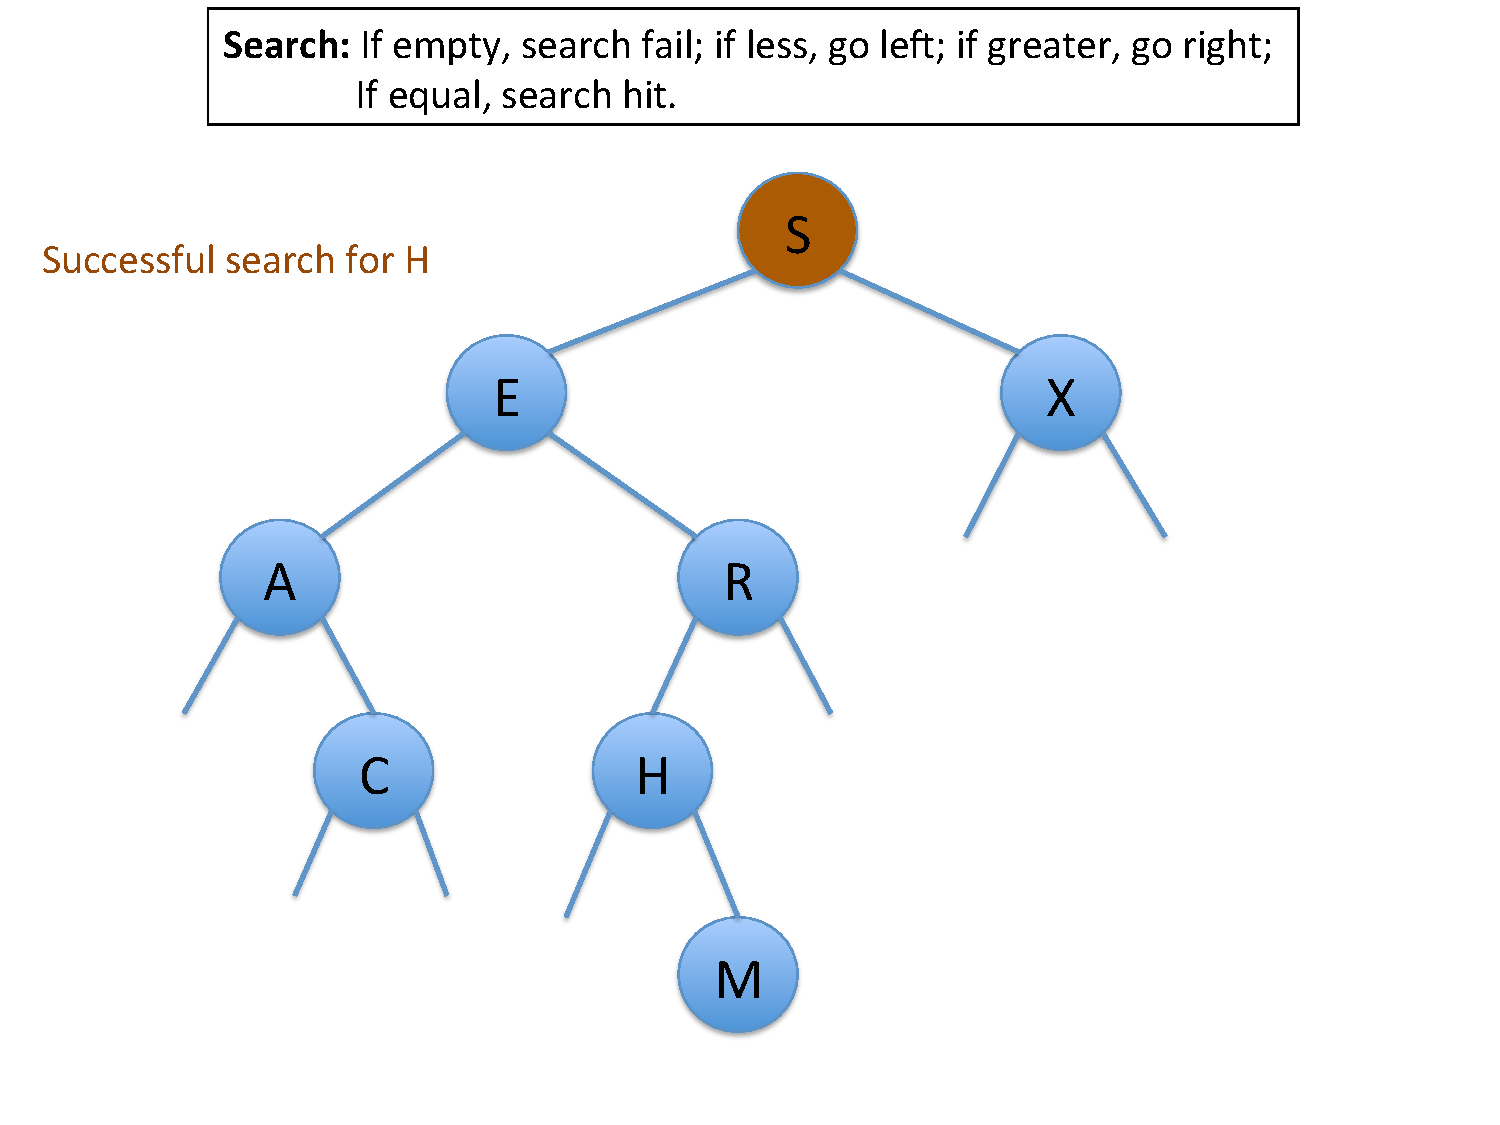
\includegraphics[width=10cm]{binary_search_tree_find2.pdf}%
%% \end{center}

%% \end{frame}

%% \begin{frame}[containsverbatim]
%% \frametitle{Binary Search Tree: Find}

%% \begin{center}
%% 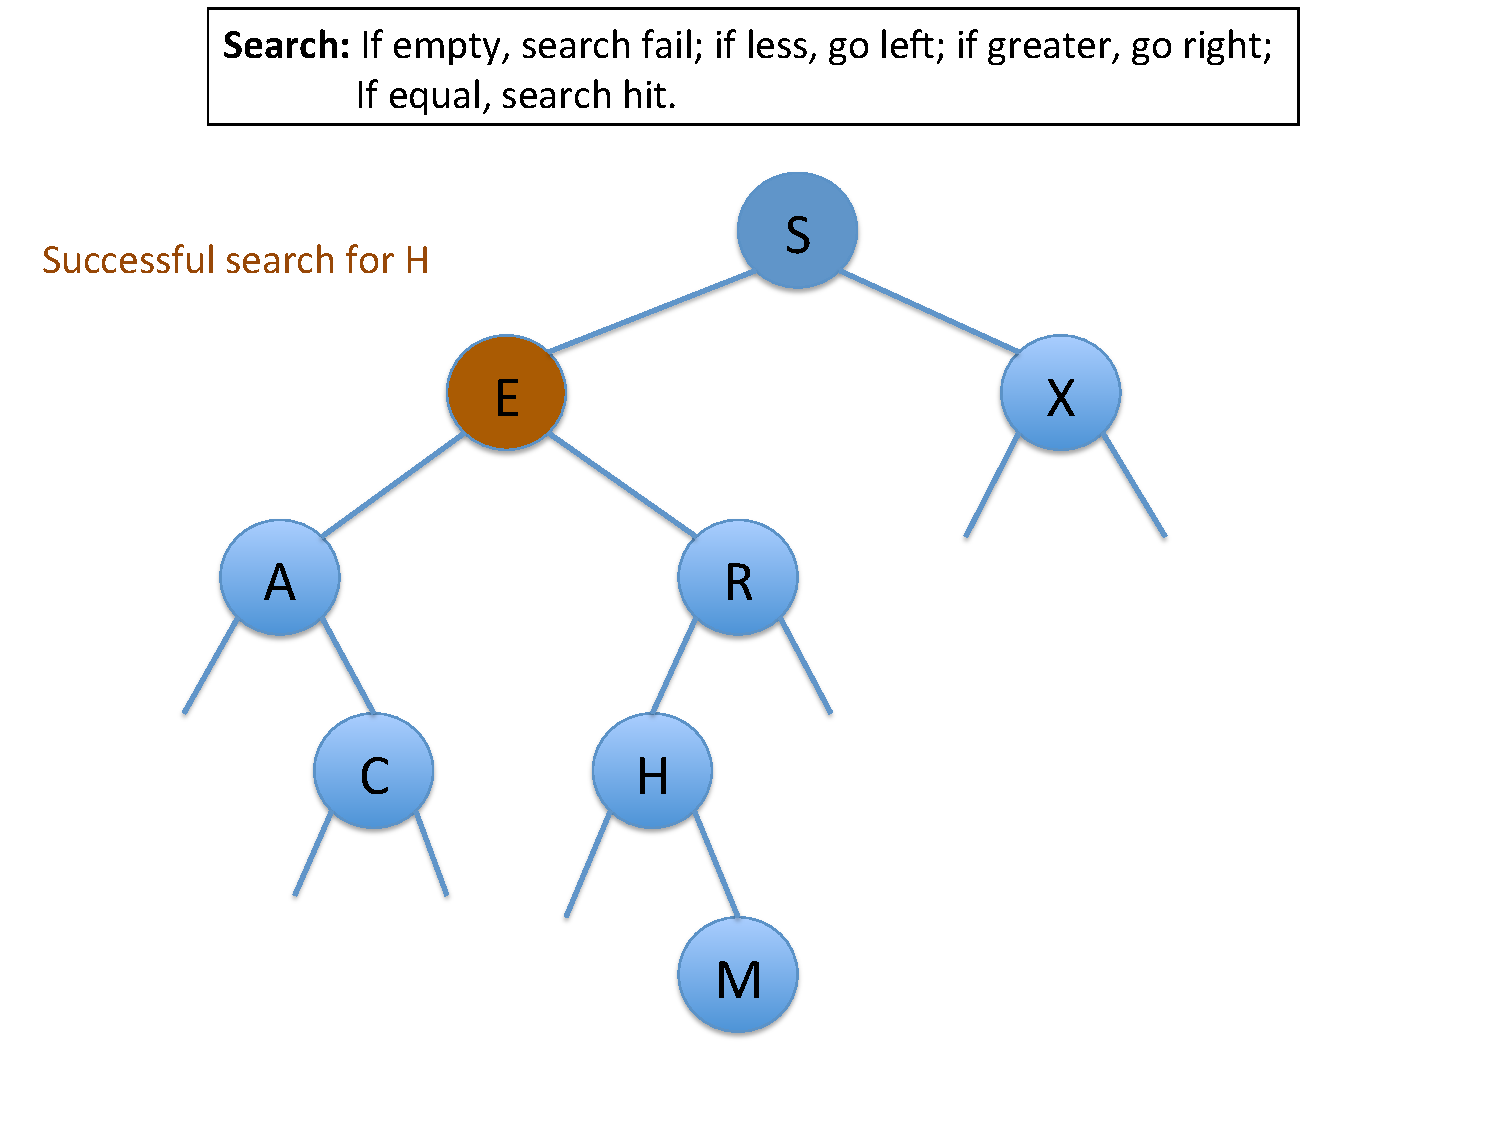
\includegraphics[width=10cm]{binary_search_tree_find3.pdf}%
%% \end{center}

%% \end{frame}

%% \begin{frame}[containsverbatim]
%% \frametitle{Binary Search Tree: Find}

%% \begin{center}
%% 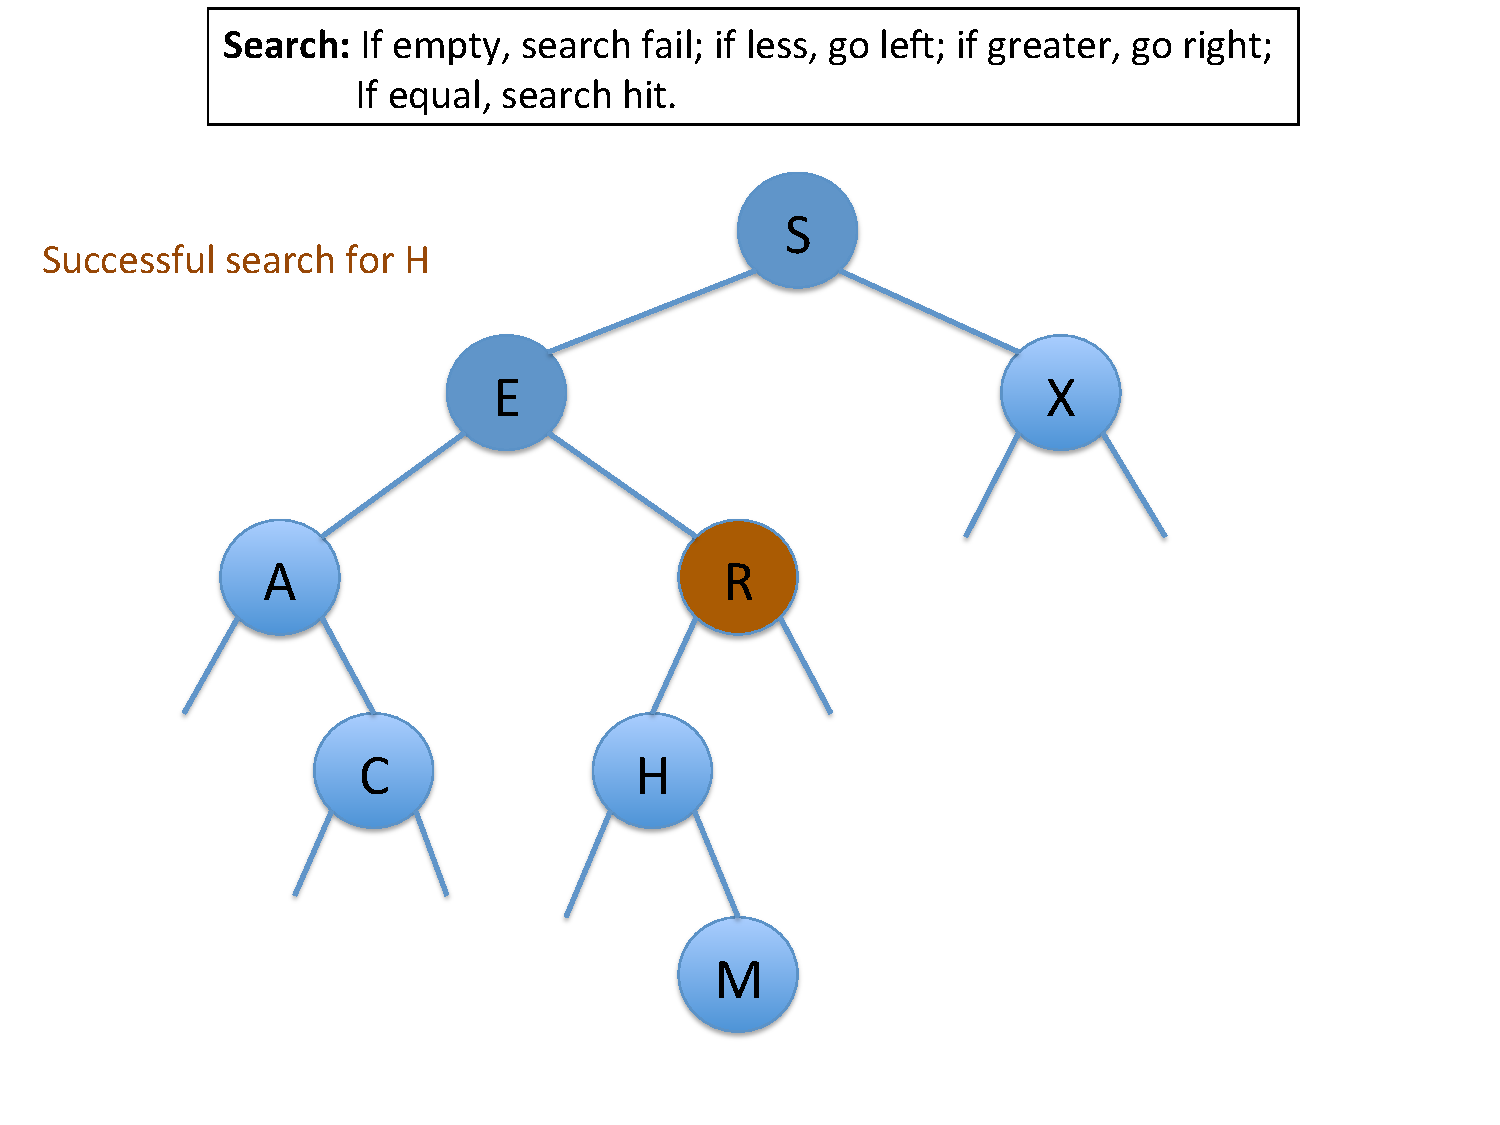
\includegraphics[width=10cm]{binary_search_tree_find4.pdf}%
%% \end{center}

%% \end{frame}

%% \begin{frame}[containsverbatim]
%% \frametitle{Binary Search Tree: Find}

%% \begin{center}
%% 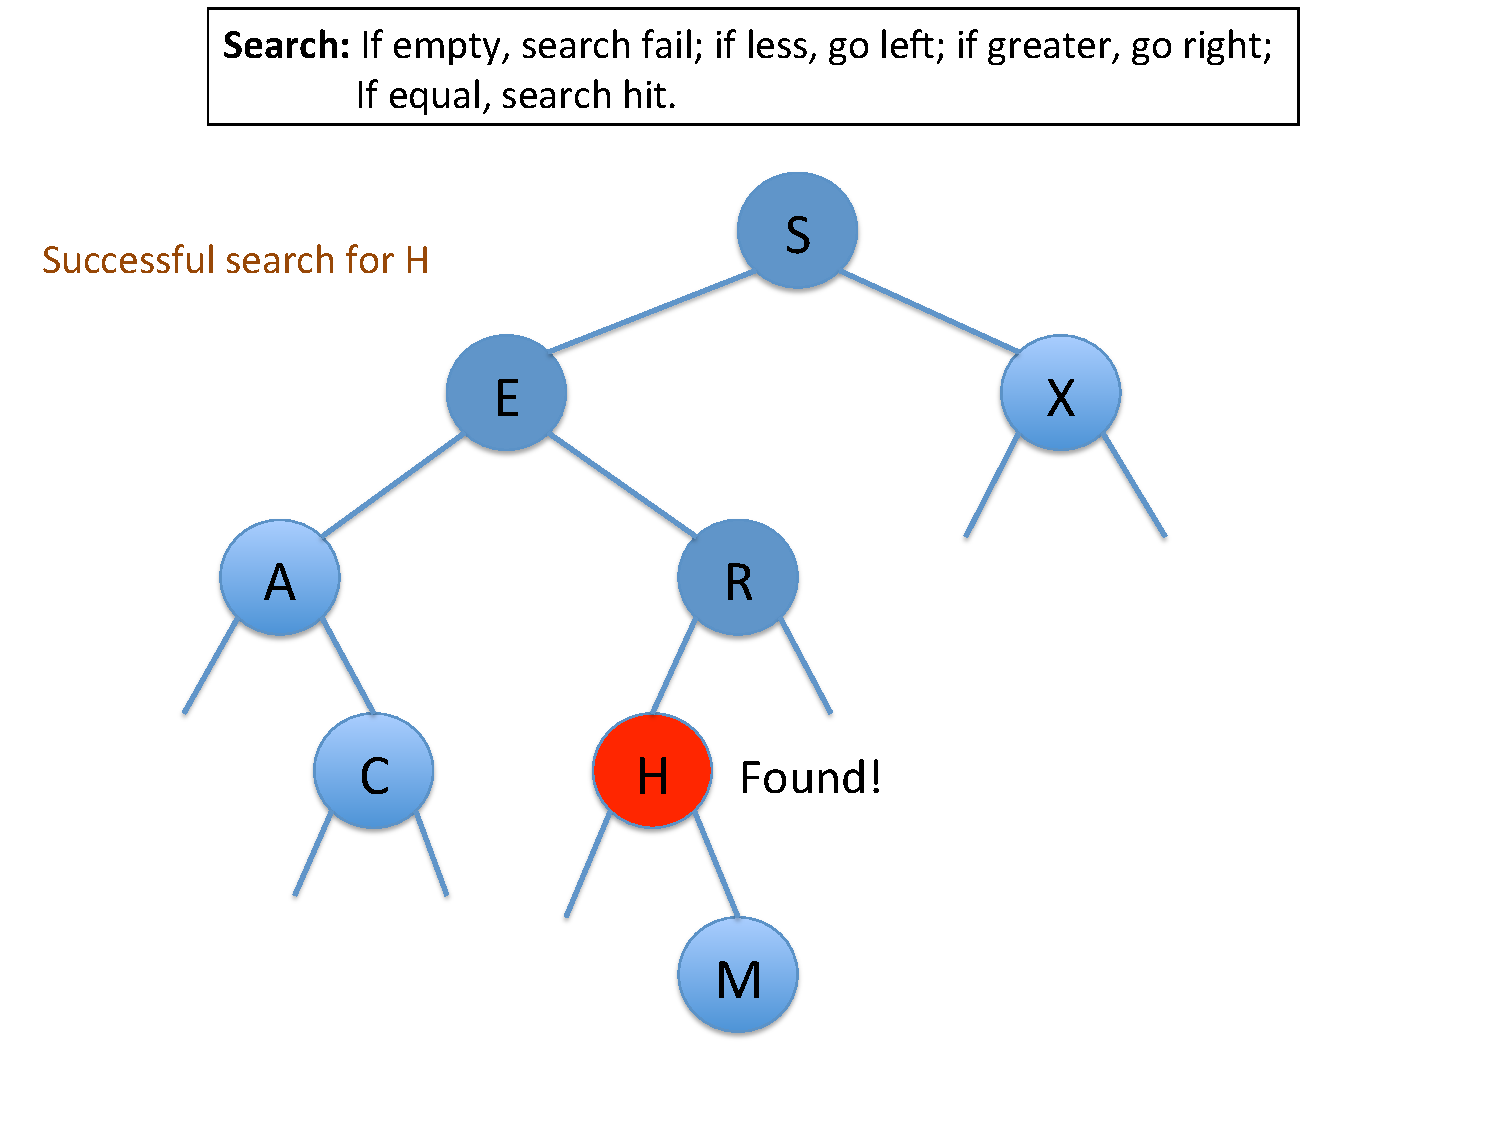
\includegraphics[width=10cm]{binary_search_tree_find5.pdf}%
%% \end{center}

%% \end{frame}

%% \begin{frame}[containsverbatim]
%% \frametitle{Binary Search Tree: Insert}

%% \begin{center}
%% 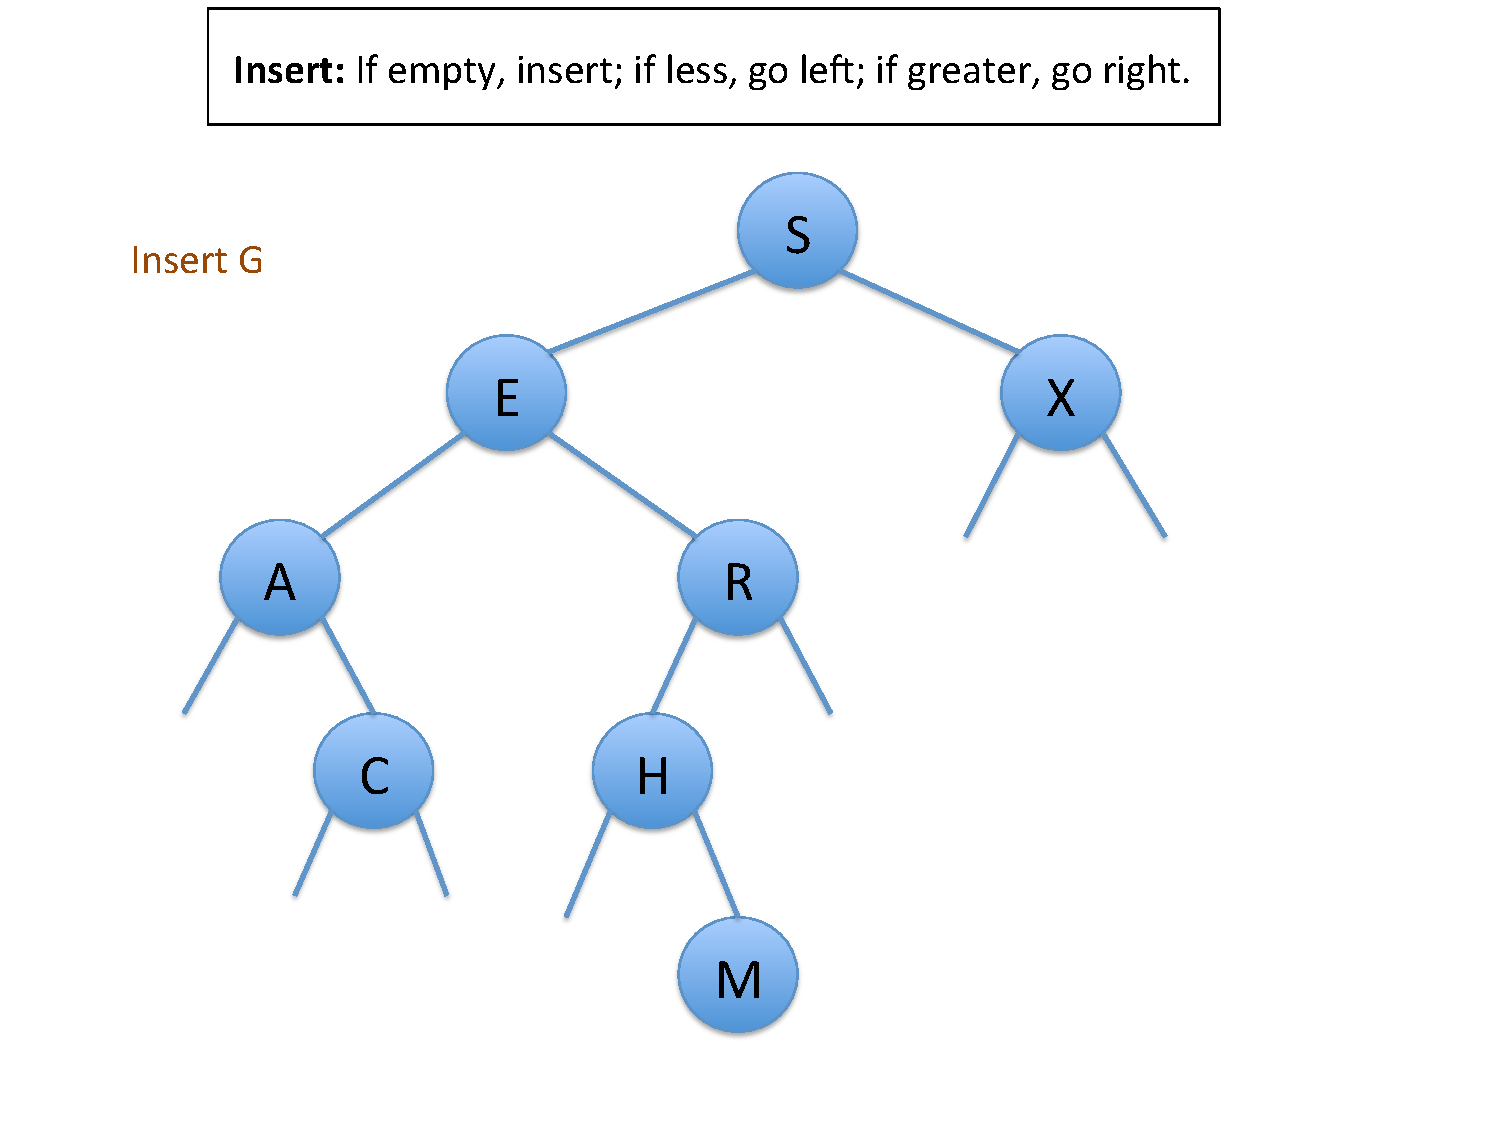
\includegraphics[width=10cm]{binary_search_tree_insert1.pdf}%
%% \end{center}

%% \end{frame}

%% \begin{frame}[containsverbatim]
%% \frametitle{Binary Search Tree: Insert}

%% \begin{center}
%% 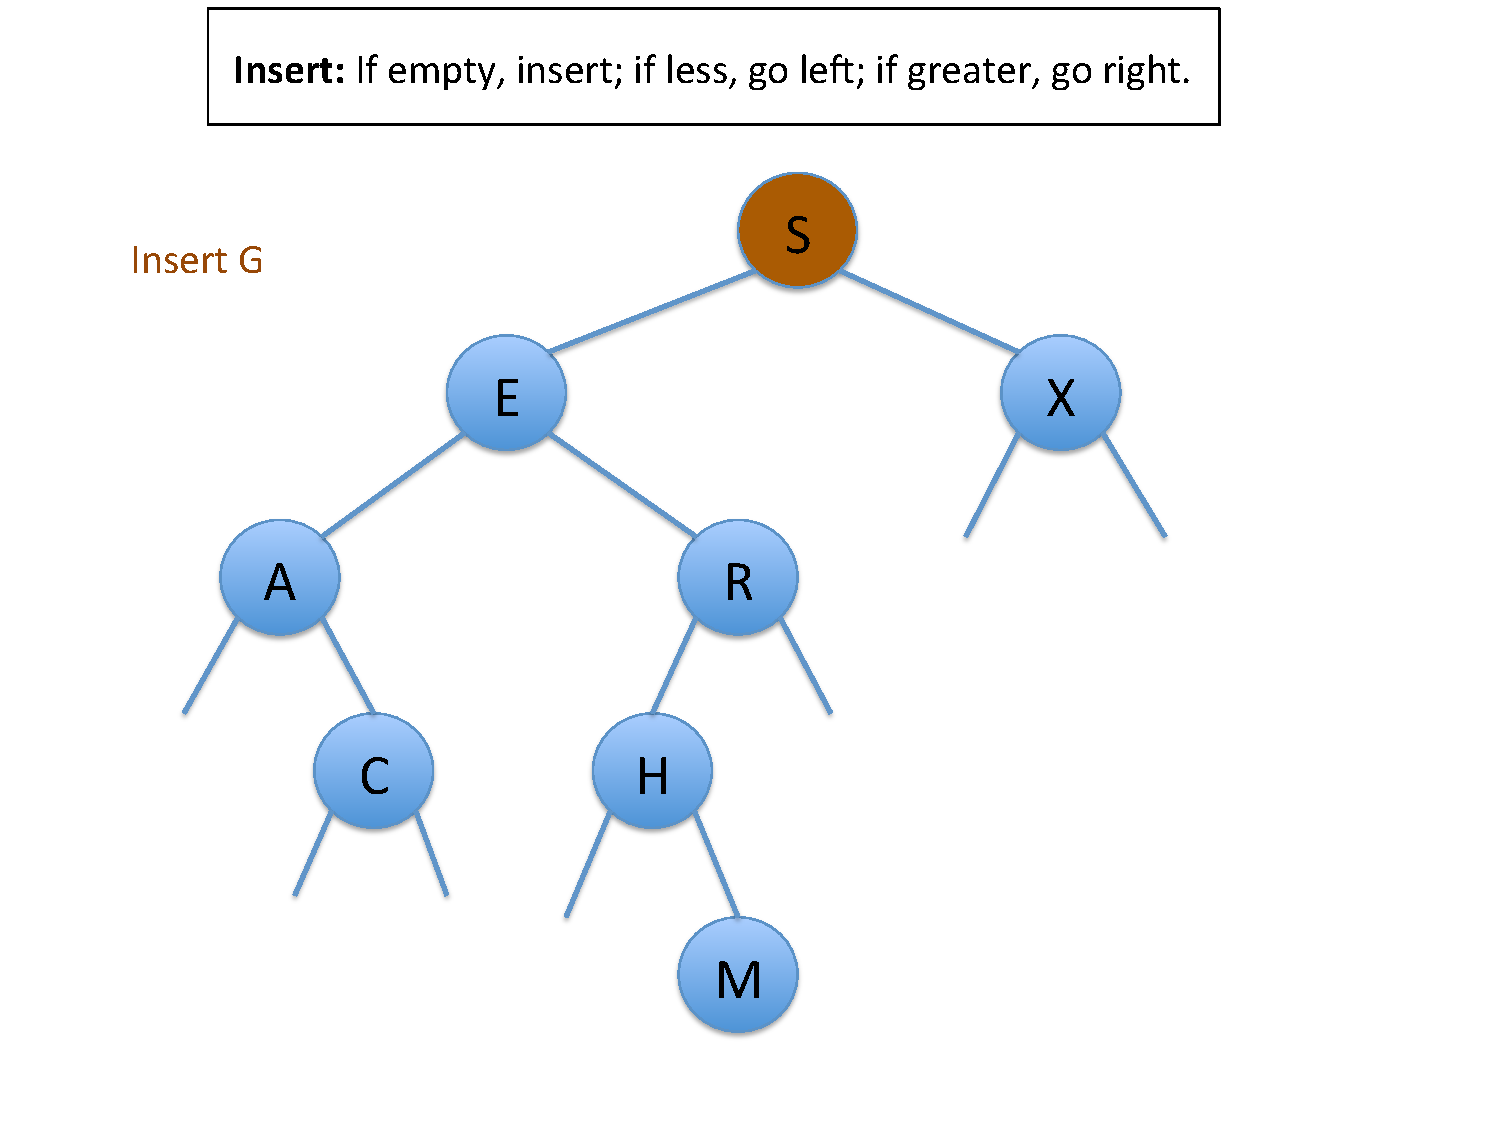
\includegraphics[width=10cm]{binary_search_tree_insert2.pdf}%
%% \end{center}

%% \end{frame}

%% \begin{frame}[containsverbatim]
%% \frametitle{Binary Search Tree: Insert}

%% \begin{center}
%% 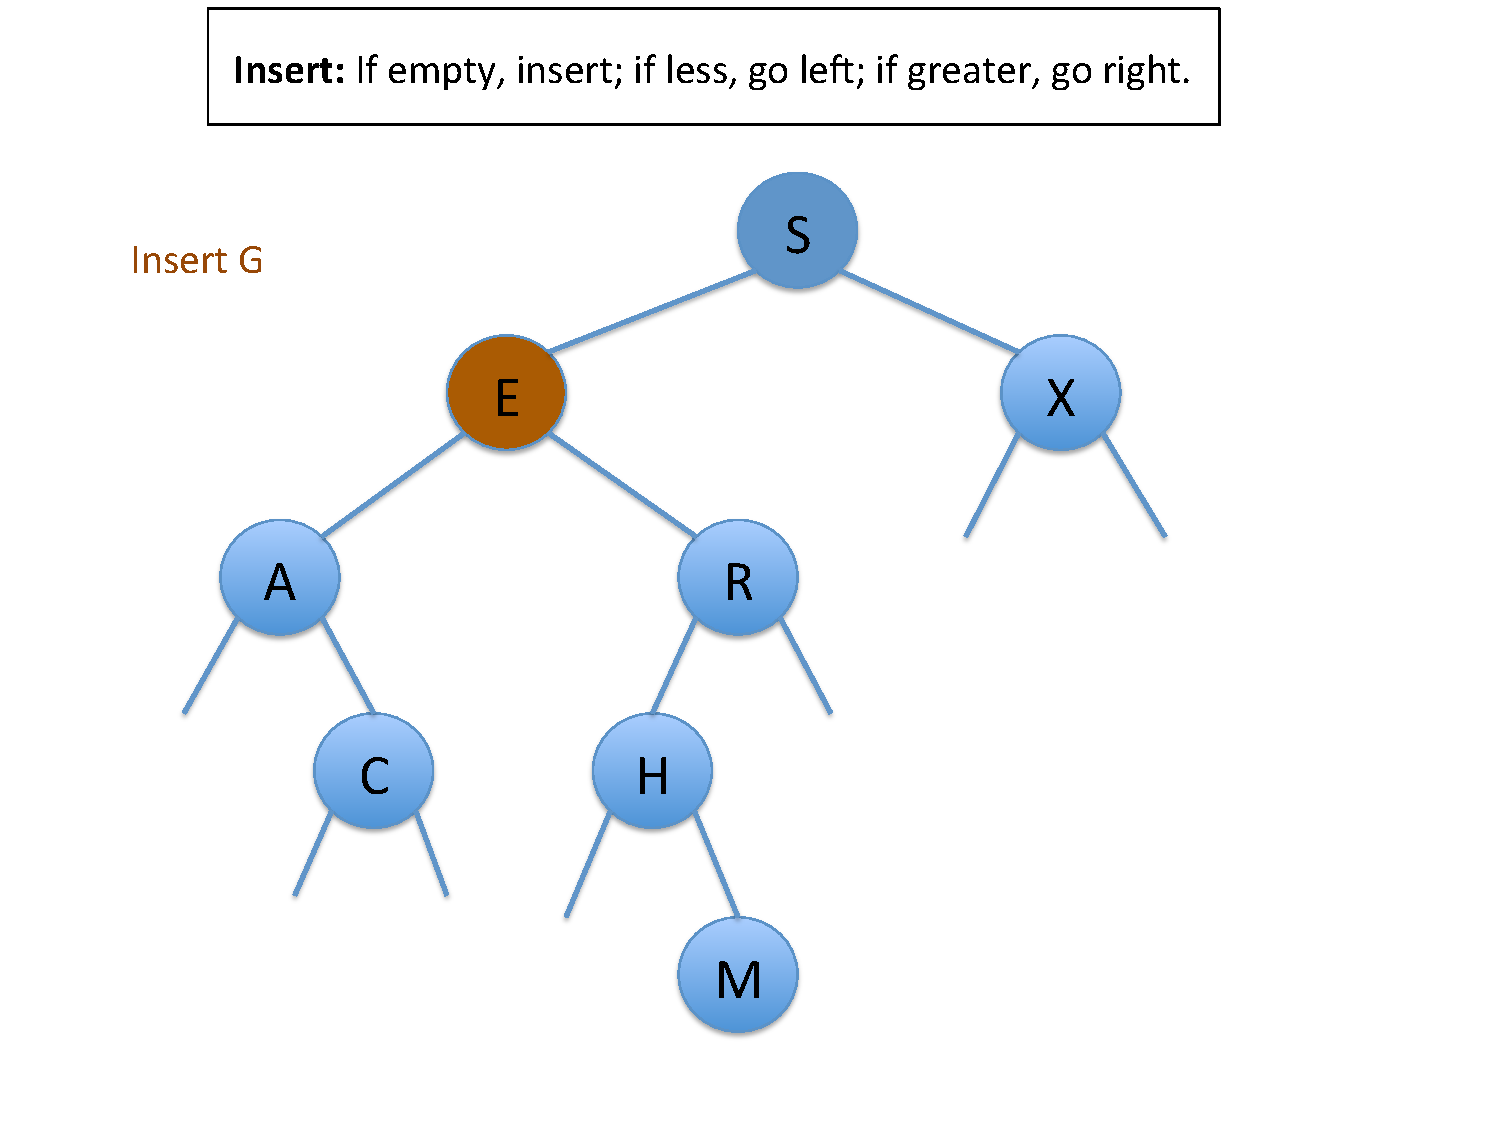
\includegraphics[width=10cm]{binary_search_tree_insert3.pdf}%
%% \end{center}

%% \end{frame}

%% \begin{frame}[containsverbatim]
%% \frametitle{Binary Search Tree: Insert}

%% \begin{center}
%% \includegraphics[width=10cm]{binary_search_tree_insert4.pdf}%
%% \end{center}

%% \end{frame}

%% \begin{frame}[containsverbatim]
%% \frametitle{Binary Search Tree: Insert}

%% \begin{center}
%% \includegraphics[width=10cm]{binary_search_tree_insert5.pdf}%
%% \end{center}

%% \end{frame}

%% \begin{frame}[containsverbatim]
%% \frametitle{Binary Search Tree: Insert}

%% \begin{center}
%% \includegraphics[width=10cm]{binary_search_tree_insert6.pdf}%
%% \end{center}

%% \end{frame}


\subsection{Fenwick Tree}

\begin{frame}%[containsverbatim]
\frametitle{Fenwick Tree}

\begin{itemize}

\item A \textbf{Fenwick Tree} is a data structure able to
\begin{itemize}
\item<1-> Compute the sum of any range of consecutive elements of an array
in $O(\log n)$.
\item<1-> Change the value of any single element in $O(\log n)$.
\end{itemize}

\vspace{0.2cm}
\item<2-> We already saw how to cache some information to compute the sum of any range
of consecutive elements of an array in $O(1)$:

\begin{overlayarea}{1\textwidth}{0.25\textheight}
\begin{center}
\includegraphics<2>[width=7.5cm]{fenwick_tree.pdf}%
\includegraphics<3>[width=7.5cm]{fenwick_tree1.pdf}%
\includegraphics<4>[width=7.5cm]{fenwick_tree2.pdf}%
\includegraphics<5>[width=7.5cm]{fenwick_tree3.pdf}%
\includegraphics<6->[width=7.5cm]{fenwick_tree4.pdf}%
\end{center}
\end{overlayarea}

\item<7-> But with our last technique, we cannot update efficiently some values in the array.

\end{itemize}

\end{frame}

\begin{frame}%[containsverbatim]
\frametitle{Representation}

%\scriptsize
%% Parts of this explanation are based on a post from \href{http://cs.stackexchange.com/questions/10538/bit-what-is-the-intuition-behind-a-binary-indexed-tree-and-how-was-it-thought-a}{\color{blue}{http://cs.stackexchange.com}}.\\

\begin{itemize}

\item With heaps and binary trees, we have seen that a tree-like data structure
can give us $O(\log(n))$ query time.

\vspace{0.3cm}

\item<2-> We can try to represent an array of size $n$ like a tree, with a range sum in each of its $n$ nodes.

\begin{overlayarea}{1\textwidth}{0.4\textheight}
\begin{center}
\includegraphics<2>[width=5cm]{fenwick_tree5.pdf}%
\includegraphics<3>[width=5cm]{fenwick_tree6.pdf}%
\end{center}
\end{overlayarea}

\end{itemize}

\end{frame}

\begin{frame}%[containsverbatim]
\frametitle{Representation}

\setbeamercovered{transparent=0}

%\scriptsize

\begin{itemize}

\item The indices on the nodes follow an in-order traversal of the tree.
\begin{center}
\includegraphics<2>[width=4cm]{fenwick_tree7.pdf}%
\includegraphics<3>[width=4cm]{fenwick_tree8.pdf}%
\includegraphics<4>[width=4cm]{fenwick_tree9.pdf}%
\includegraphics<5>[width=4cm]{fenwick_tree10.pdf}%
\includegraphics<6>[width=4cm]{fenwick_tree11.pdf}%
\includegraphics<7>[width=4cm]{fenwick_tree12.pdf}%
\includegraphics<8>[width=4cm]{fenwick_tree13.pdf}%
\includegraphics<9>[width=4cm]{fenwick_tree14.pdf}%
\end{center}

\item<10-> We define $lleaf(k)$ as the index of the left most leaf of the node of index $k$.
\begin{center}
\includegraphics<11>[width=4cm]{fenwick_tree6.pdf}%
\includegraphics<12>[width=4cm]{fenwick_tree15.pdf}%
\includegraphics<13>[width=4cm]{fenwick_tree16.pdf}%
\end{center}

\item<14-> The value of a given node of index $k$ is $\sum_{i=lleaf(k)}^k \texttt{array[i]}$.
\begin{center}
\includegraphics<15>[width=4cm]{fenwick_tree6.pdf}%
\includegraphics<16>[width=4cm]{fenwick_tree15.pdf}%
\includegraphics<17>[width=4cm]{fenwick_tree17.pdf}%
\includegraphics<18>[width=4cm]{fenwick_tree6.pdf}%
\includegraphics<19>[width=4cm]{fenwick_tree18.pdf}%
\includegraphics<20>[width=4cm]{fenwick_tree19.pdf}%
\includegraphics<21>[width=4cm]{fenwick_tree6.pdf}%
\includegraphics<22>[width=4cm]{fenwick_tree20.pdf}%
\includegraphics<23>[width=4cm]{fenwick_tree21.pdf}%
\end{center}

\end{itemize}

\end{frame}


\begin{frame}%[containsverbatim]
\frametitle{Range Value}

To compute the sum of the range $[0..k]$ we do the following:

\vspace{0.2cm}

\begin{enumerate}
\item<1-> Set a \texttt{sum} variable to $0$.

\vspace{0.2cm}

\item<2-> Go to the node of index $k$ and add its value to \texttt{sum}.

\vspace{0.2cm}

\item<3-> If the current node is the root stop. Otherwise, go to the parent node and,
\begin{itemize}
\item<4-> If we get to the parent from its left branch, add nothing to \texttt{sum}.
\item<5-> If we get to the parent from its right branch, add the value of the parent to \texttt{sum}.
\end{itemize}

\vspace{0.2cm}

\item<6-> Goto 3.
\end{enumerate}

\end{frame}

\begin{frame}%[containsverbatim]
\frametitle{Range Value}

\begin{center}
\includegraphics<1>[width=9cm]{fenwick_tree22.pdf}%
\includegraphics<2>[width=9cm]{fenwick_tree23.pdf}%
\includegraphics<3>[width=9cm]{fenwick_tree24.pdf}%
\includegraphics<4>[width=9cm]{fenwick_tree25.pdf}%
\includegraphics<5>[width=9cm]{fenwick_tree26.pdf}%
\includegraphics<6>[width=9cm]{fenwick_tree27.pdf}%
\includegraphics<7>[width=9cm]{fenwick_tree28.pdf}%
\includegraphics<8>[width=9cm]{fenwick_tree29.pdf}%
\includegraphics<9>[width=9cm]{fenwick_tree22.pdf}%
\includegraphics<10>[width=9cm]{fenwick_tree30.pdf}%
\includegraphics<11>[width=9cm]{fenwick_tree31.pdf}%
\includegraphics<12>[width=9cm]{fenwick_tree32.pdf}%
\includegraphics<13>[width=9cm]{fenwick_tree33.pdf}%
\includegraphics<14>[width=9cm]{fenwick_tree34.pdf}%
\includegraphics<15>[width=9cm]{fenwick_tree35.pdf}%
\includegraphics<16>[width=9cm]{fenwick_tree36.pdf}%
\includegraphics<17>[width=9cm]{fenwick_tree37.pdf}%
\end{center}

\end{frame}

\begin{frame}%[containsverbatim]
\frametitle{Update Value}

To increase the value at index $k$ of the array by $\Delta$, we do the following:

\vspace{0.2cm}

\begin{enumerate}
\item<2-> Go to the node of index $k$.

\vspace{0.2cm}

\item<3-> Add $\Delta$ to the current node and
\begin{itemize}
\item<4-> If we can reach the parent by its left branch, go to the parent node and goto 2.
\vspace{0.1cm}
\item<5-> Otherwise stop.
\end{itemize}

\end{enumerate}

\end{frame}

\begin{frame}%[containsverbatim]
\frametitle{Update Value}

\begin{center}
\includegraphics<1>[width=9cm]{fenwick_tree22.pdf}%
\includegraphics<2>[width=9cm]{fenwick_tree38.pdf}%
\includegraphics<3>[width=9cm]{fenwick_tree39.pdf}%
\includegraphics<4>[width=9cm]{fenwick_tree40.pdf}%
\includegraphics<5>[width=9cm]{fenwick_tree41.pdf}%
\includegraphics<6>[width=9cm]{fenwick_tree42.pdf}%
\includegraphics<7>[width=9cm]{fenwick_tree43.pdf}%
\includegraphics<8>[width=9cm]{fenwick_tree44.pdf}%
\includegraphics<9>[width=9cm]{fenwick_tree45.pdf}%
\includegraphics<10>[width=9cm]{fenwick_tree46.pdf}%
\includegraphics<11>[width=9cm]{fenwick_tree47.pdf}%
\includegraphics<12>[width=9cm]{fenwick_tree48.pdf}%
\includegraphics<13>[width=9cm]{fenwick_tree49.pdf}%
\includegraphics<14>[width=9cm]{fenwick_tree50.pdf}%
\includegraphics<15>[width=9cm]{fenwick_tree51.pdf}%
\includegraphics<16>[width=9cm]{fenwick_tree52.pdf}%
\includegraphics<17>[width=9cm]{fenwick_tree53.pdf}%
\includegraphics<18>[width=9cm]{fenwick_tree54.pdf}%
\includegraphics<19>[width=9cm]{fenwick_tree55.pdf}%
\includegraphics<20>[width=9cm]{fenwick_tree55_1.pdf}%
\end{center}

\end{frame}

\begin{frame}%[containsverbatim]
\frametitle{Traversing the Tree Efficiently}
\footnotesize
\textbf{Range value:} To compute the sum of the range $[0..k]$, starting from a node $k$ we can get the
indices of the nodes involved in the sum using
\begin{itemize}
\footnotesize
\item<1-> \texttt{k = (k \& (k + 1)) - 1}.
%\vspace{0.06cm}
\item<1-> Or, \texttt{k = k - (k \& -k)}.
\end{itemize}

\vspace{-0.15cm}

\begin{overlayarea}{1\textwidth}{0.85\textheight}
\begin{center}
\includegraphics<2>[width=8cm]{fenwick_tree22.pdf}%
\includegraphics<3>[width=8cm]{fenwick_tree56.pdf}%
\includegraphics<4>[width=8cm]{fenwick_tree57.pdf}%
\includegraphics<5>[width=8cm]{fenwick_tree58.pdf}%
\includegraphics<6>[width=8cm]{fenwick_tree59.pdf}%
\includegraphics<7>[width=8cm]{fenwick_tree60.pdf}%
\includegraphics<8>[width=8cm]{fenwick_tree61.pdf}%
\includegraphics<9>[width=8cm]{fenwick_tree62.pdf}%
\includegraphics<10>[width=8cm]{fenwick_tree63.pdf}%
\includegraphics<11>[width=8cm]{fenwick_tree64.pdf}%
\includegraphics<12>[width=8cm]{fenwick_tree65.pdf}%
\includegraphics<13>[width=8cm]{fenwick_tree66.pdf}%
\end{center}
\end{overlayarea}

\end{frame}

\begin{frame}%[containsverbatim]
\frametitle{Traversing the Tree Efficiently}

\footnotesize
%\begin{itemize}

\textbf{Update value:} To update the value at index $k$, starting from a node $k$ we can get the
indices of the nodes involved using
\begin{itemize}
\footnotesize
%\vspace{0.1cm}
\item<1-> \texttt{k = k | (k + 1)}.
%\vspace{0.06cm}
\item<1-> Or, \texttt{k = k + (k \& -k)}.
\end{itemize}

%\end{itemize}

\vspace{-0.1cm}

\begin{overlayarea}{1\textwidth}{0.88\textheight}
\begin{center}
\includegraphics<2>[width=8cm]{fenwick_tree22.pdf}%
\includegraphics<3>[width=8cm]{fenwick_tree56.pdf}%
\includegraphics<4>[width=8cm]{fenwick_tree67.pdf}%
\includegraphics<5>[width=8cm]{fenwick_tree68.pdf}%
\includegraphics<6>[width=8cm]{fenwick_tree68bis.pdf}%
\includegraphics<7>[width=8cm]{fenwick_tree69.pdf}%
\includegraphics<8>[width=8cm]{fenwick_tree70.pdf}%
\includegraphics<9>[width=8cm]{fenwick_tree71.pdf}%
\includegraphics<10>[width=8cm]{fenwick_tree72.pdf}%
\includegraphics<11>[width=8cm]{fenwick_tree73.pdf}%
\includegraphics<12>[width=8cm]{fenwick_tree74.pdf}%
\includegraphics<13>[width=8cm]{fenwick_tree75.pdf}%
\end{center}
\end{overlayarea}

\end{frame}

\begin{frame}[containsverbatim]
\frametitle{Fenwick Tree Implementation}

\scriptsize

\begin{lstlisting}[mathescape]
class fenwick_tree {
  vector<int> tree;
public:
  fenwick_tree(const vector<int>& array) : tree(array.size(), 0)
  {
    for (unsigned int i = 0; i < tree.size(); ++i)
    {
      increase(i, array[i]);
    }
  }

  void increase(int i, int delta)
  {
    for (; i < (int)tree.size(); i |= i + 1)
    {
      tree[i] += delta;
    }
  }
  // ...
\end{lstlisting}

\end{frame}

\begin{frame}[containsverbatim]
\frametitle{Fenwick Tree Implementation}

\scriptsize

\begin{lstlisting}[mathescape]
  // ...
  int get_sum(int left, int right)
  {
    return sum(right) - sum(left - 1);
  }

  int sum(int ind)
  {
    int sum = 0;
    while (ind >= 0)
    {
      sum += tree[ind];
      ind &= ind + 1;
      --ind;
    }
    return sum;
  }
};
\end{lstlisting}

\end{frame}

\begin{frame}%[containsverbatim]
\frametitle{\exo}

\spojlink{It's a Murder!}{http://www.spoj.com/problems/DCEPC206/}

\end{frame}

\ifanswers

\begin{frame}%[containsverbatim]
\frametitle{Solution}

\setbeamercovered{transparent=0}

\begin{itemize}

\item If the constraints were small, the problem would be very easy: Just simulate the process.

\begin{overlayarea}{1\textwidth}{0.3\textheight}
\begin{center}
\includegraphics<2>[width=8cm]{its_a_murder.pdf}%
\includegraphics<3>[width=8cm]{its_a_murder1.pdf}%
\includegraphics<4>[width=8cm]{its_a_murder2.pdf}%
\includegraphics<5>[width=8cm]{its_a_murder3.pdf}%
\includegraphics<6>[width=8cm]{its_a_murder4.pdf}%
\includegraphics<7>[width=8cm]{its_a_murder5.pdf}%
\includegraphics<8>[width=8cm]{its_a_murder6.pdf}%
\includegraphics<9>[width=8cm]{its_a_murder7.pdf}%
\includegraphics<10>[width=8cm]{its_a_murder8.pdf}%
\includegraphics<11>[width=8cm]{its_a_murder9.pdf}%
\includegraphics<12>[width=8cm]{its_a_murder10.pdf}%
\includegraphics<13>[width=8cm]{its_a_murder11.pdf}%
\includegraphics<14>[width=8cm]{its_a_murder12.pdf}%
\includegraphics<15>[width=8cm]{its_a_murder13.pdf}%
\includegraphics<16>[width=8cm]{its_a_murder14.pdf}%
\includegraphics<17->[width=8cm]{its_a_murder15.pdf}%
\end{center}
\end{overlayarea}

\item<18-> But this gives rise to a quadratic complexity.

\vspace{0.2cm}

\item<19-> Can we get a complexity of $O(n\log n)$ to pass the constraints?

\end{itemize}

\end{frame}

\begin{frame}%[containsverbatim]
\frametitle{Solution}

\footnotesize

Going from left to right, we can use a fenwick tree to store the sum of elements less than a given number.

\begin{overlayarea}{1\textwidth}{0.85\textheight}
\begin{center}
\includegraphics<2>[width=8cm]{its_a_murder16.pdf}%
\includegraphics<3>[width=8cm]{its_a_murder17.pdf}%
\includegraphics<4>[width=8cm]{its_a_murder18.pdf}%
\includegraphics<5>[width=8cm]{its_a_murder19.pdf}%
\includegraphics<6>[width=8cm]{its_a_murder20.pdf}%
\includegraphics<7>[width=8cm]{its_a_murder21.pdf}%
\includegraphics<8>[width=8cm]{its_a_murder22.pdf}%
\includegraphics<9>[width=8cm]{its_a_murder23.pdf}%
\includegraphics<10>[width=8cm]{its_a_murder24.pdf}%
\includegraphics<11>[width=8cm]{its_a_murder25.pdf}%
\includegraphics<12>[width=8cm]{its_a_murder26.pdf}%
\includegraphics<13>[width=8cm]{its_a_murder27.pdf}%
\includegraphics<14>[width=8cm]{its_a_murder28.pdf}%
\includegraphics<15>[width=8cm]{its_a_murder29.pdf}%
\includegraphics<16>[width=8cm]{its_a_murder30.pdf}%
\includegraphics<17>[width=8cm]{its_a_murder31.pdf}%
\includegraphics<18>[width=8cm]{its_a_murder32.pdf}%
\includegraphics<19>[width=8cm]{its_a_murder33.pdf}%
\includegraphics<20>[width=8cm]{its_a_murder34.pdf}%
\includegraphics<21>[width=8cm]{its_a_murder35.pdf}%
\includegraphics<22>[width=8cm]{its_a_murder36.pdf}%
\includegraphics<23>[width=8cm]{its_a_murder37.pdf}%
%\includegraphics<24>[width=8cm]{its_a_murder38.pdf}%
\includegraphics<24>[width=8cm]{its_a_murder39.pdf}%
\includegraphics<25>[width=8cm]{its_a_murder40.pdf}%
\includegraphics<26>[width=8cm]{its_a_murder41.pdf}%
\includegraphics<27>[width=8cm]{its_a_murder42.pdf}%
\includegraphics<28>[width=8cm]{its_a_murder43.pdf}%
\includegraphics<29>[width=8cm]{its_a_murder44.pdf}%
\end{center}
\end{overlayarea}

\end{frame}

\begin{frame}[containsverbatim]
\frametitle{Solution Implementation}

\scriptsize

\begin{lstlisting}[mathescape]
int main(int argc, char *argv[]) {
  int tc;
  cin >> tc;
  while (tc--)
  {
    int N;
    cin >> N;
    fenwick_tree ft(1e6 + 1);
    long long res = 0;
    for (int i = 0; i < N; ++i)
    {
      int v;
      cin >> v;
      res += ft.get_sum(0, v - 1);
      ft.increase(v, v);
    }
    cout << res << endl;
  }
  return 0;
}
\end{lstlisting}

\end{frame}

\begin{frame}[containsverbatim]
\frametitle{Solution Implementation}

\scriptsize

\begin{lstlisting}[mathescape]
class fenwick_tree {
  vector<long long> tree;

public:
  // ...
  long long get_sum(int left, int right) {
    return sum(right) - sum(left - 1);
  }

  long long sum(int ind) {
    long long sum = 0;
    while (ind >= 0)
    {
      sum += tree[ind];
      ind &= ind + 1;
      ind--;
    }
    return sum;
  }
};
\end{lstlisting}

\end{frame}

\fi

\begin{frame}%[containsverbatim]
\frametitle{\exo}
\label{slides:lightOJ_1085}
\lightojlink{1085}{http://www.lightoj.com/volume_showproblem.php?problem=1085}

\vspace{1cm}

\hint{Have a look at the \hyperlink{slide:LIS}{\emph{LIS}} part of the dynamic programming section.}

\end{frame}

\ifanswers

\begin{frame}%[containsverbatim]
\frametitle{Solution}

\setbeamercovered{transparent=0}

\begin{itemize}

\item We can modify the \emph{LIS} algorithm we developped (in the dynamic programming part),
to count the number of increasing subsequences.

\begin{overlayarea}{1\textwidth}{0.45\textheight}
\begin{center}
\includegraphics<2>[width=8cm]{lis_number.pdf}%
\includegraphics<3>[width=8cm]{lis_number1.pdf}%
\includegraphics<4>[width=8cm]{lis_number2.pdf}%
\includegraphics<5>[width=8cm]{lis_number3.pdf}%
\includegraphics<6>[width=8cm]{lis_number4.pdf}%
\includegraphics<7>[width=8cm]{lis_number5.pdf}%
\includegraphics<8>[width=8cm]{lis_number6.pdf}%
\includegraphics<9>[width=8cm]{lis_number7.pdf}%
\includegraphics<10>[width=8cm]{lis_number8.pdf}%
\includegraphics<11>[width=8cm]{lis_number9.pdf}%
\includegraphics<12>[width=8cm]{lis_number10.pdf}%
\includegraphics<13>[width=8cm]{lis_number11.pdf}%
\includegraphics<14>[width=8cm]{lis_number12.pdf}%
\includegraphics<15>[width=8cm]{lis_number13.pdf}%
\includegraphics<16>[width=8cm]{lis_number14.pdf}%
\includegraphics<17>[width=8cm]{lis_number15.pdf}%
\includegraphics<18>[width=8cm]{lis_number16.pdf}%
\includegraphics<19>[width=8cm]{lis_number17.pdf}%
\includegraphics<20>[width=8cm]{lis_number18.pdf}%
\includegraphics<21>[width=8cm]{lis_number19.pdf}%
\includegraphics<22>[width=8cm]{lis_number20.pdf}%
\includegraphics<23>[width=8cm]{lis_number21.pdf}%
\includegraphics<24>[width=8cm]{lis_number22.pdf}%
\includegraphics<25>[width=8cm]{lis_number23.pdf}%
\includegraphics<26>[width=8cm]{lis_number24.pdf}%
\includegraphics<27>[width=8cm]{lis_number25.pdf}%
\includegraphics<28>[width=8cm]{lis_number26.pdf}%
\includegraphics<29>[width=8cm]{lis_number27.pdf}%
\includegraphics<30>[width=8cm]{lis_number28.pdf}%
%\includegraphics<31>[width=8cm]{lis_number29.pdf}%
\includegraphics<31>[width=8cm]{lis_number30.pdf}%
\includegraphics<32>[width=8cm]{lis_number31.pdf}%
\includegraphics<33>[width=8cm]{lis_number32.pdf}%
\includegraphics<34>[width=8cm]{lis_number33.pdf}%
\includegraphics<35>[width=8cm]{lis_number34.pdf}%
\includegraphics<36>[width=8cm]{lis_number35.pdf}%
\includegraphics<37>[width=8cm]{lis_number36.pdf}%
\includegraphics<38>[width=8cm]{lis_number37.pdf}%
\includegraphics<39->[width=8cm]{lis_number38.pdf}%
\end{center}
\end{overlayarea}

\item<40-> But we get a quadratic complexity, not fast enough for the current constraints.


\end{itemize}

\end{frame}

\begin{frame}%[containsverbatim]
\frametitle{Solution}

\setbeamercovered{transparent=0}

\begin{itemize}

\item Simpler problem: If the elements of the array were sorted in increasing order, the problem would be easy.

\begin{overlayarea}{1\textwidth}{0.45\textheight}
\begin{center}
\includegraphics<2>[width=8.5cm]{lis_number39.pdf}%
\includegraphics<3->[width=8.5cm]{lis_number40.pdf}%
\end{center}
\end{overlayarea}

\item<4-> We can nearly transform the original problem in this simpler setting using pair of values and indices.

\end{itemize}

\end{frame}

\begin{frame}%[containsverbatim]
\frametitle{Solution}

\begin{center}
\includegraphics<1>[width=10.3cm]{lis_number41.pdf}%
\includegraphics<2>[width=10.3cm]{lis_number42.pdf}%
\includegraphics<3>[width=10.3cm]{lis_number43.pdf}%
\includegraphics<4>[width=10.3cm]{lis_number44.pdf}%
%\includegraphics<5>[width=10.3cm]{lis_number45.pdf}%
\includegraphics<5>[width=10.3cm]{lis_number46.pdf}%
\includegraphics<6>[width=10.3cm]{lis_number47.pdf}%
\includegraphics<7>[width=10.3cm]{lis_number48.pdf}%
\includegraphics<8>[width=10.3cm]{lis_number49.pdf}%
\includegraphics<9>[width=10.3cm]{lis_number50.pdf}%
\includegraphics<10>[width=10.3cm]{lis_number51.pdf}%
\includegraphics<11>[width=10.3cm]{lis_number52.pdf}%
\includegraphics<12>[width=10.3cm]{lis_number53.pdf}%
\includegraphics<13>[width=10.3cm]{lis_number54.pdf}%
\includegraphics<14>[width=10.3cm]{lis_number55.pdf}%
\includegraphics<15>[width=10.3cm]{lis_number56.pdf}%
\includegraphics<16>[width=10.3cm]{lis_number57.pdf}%
\includegraphics<17>[width=10.3cm]{lis_number58.pdf}%
\includegraphics<18>[width=10.3cm]{lis_number59.pdf}%
\includegraphics<19>[width=10.3cm]{lis_number60.pdf}%
\includegraphics<20>[width=10.3cm]{lis_number61.pdf}%
\includegraphics<21>[width=10.3cm]{lis_number61bis.pdf}%
\includegraphics<22>[width=10.3cm]{lis_number62.pdf}%
\includegraphics<23>[width=10.3cm]{lis_number63.pdf}%
\includegraphics<24>[width=10.3cm]{lis_number64.pdf}%
\end{center}

\end{frame}

\begin{frame}[containsverbatim]
\frametitle{Solution Implementation}

\scriptsize

\begin{lstlisting}[mathescape]
const int MOD = 1000000007;

int main(int argc, char *argv[])
{
  int TC;
  cin >> TC;
  for (int tc = 1; tc <= TC; ++tc)
  {
    int N;
    cin >> N;
    vector<pair<int, int>> value_index(N);
    for (int i = 0; i < N; ++i)
    {
      cin >> value_index[i].first;
      value_index[i].second = i;
    }
    // ...
\end{lstlisting}

\end{frame}

\begin{frame}[containsverbatim]
\frametitle{Solution Implementation}

\scriptsize

\begin{lstlisting}[mathescape]
    // ...
    auto comp = [](const pair<int, int>& p1, const pair<int, int>& p2) {
      return p1.first < p2.first ||
            (p1.first == p2.first && p1.second > p2.second);
    };
    sort(value_index.begin(), value_index.end(), comp);
    fenwick_tree ft(N);
    int res = 0;
    for (int i = 0; i < N; ++i)
    {
      int index = value_index[i].second;
      int v = ft.get_sum(0, index - 1) + 1;
      res = (res + v) % MOD;
      ft.increase(index, v);
    }
    cout << "Case " << tc << ": " << res << endl;
  }
  return 0;
}
\end{lstlisting}

\end{frame}

\begin{frame}[containsverbatim]
\frametitle{Solution Implementation}

\scriptsize

\begin{lstlisting}[mathescape]
class fenwick_tree {
  // ...
  void increase(int i, int delta)
  {
    for (; i < (int)tree.size(); i |= i + 1)
      tree[i] = (tree[i] + delta) % MOD;
  }

  int sum(int ind)
  {
    int sum = 0;
    while (ind >= 0)
    {
      sum = (sum + tree[ind]) % MOD;
      ind &= ind + 1;
      ind--;
    }
    return sum;
  }
};
\end{lstlisting}

\end{frame}

\fi

\begin{frame}%[containsverbatim]
\frametitle{\exo}

\uvalink{12365}{https://uva.onlinejudge.org/index.php?option=com_onlinejudge&Itemid=8&category=24&page=show_problem&problem=3787}

\vspace{1cm}

\hint{Have a look at modular arithmetic in the mathematics section of volume \Rmnum{2}.}

\end{frame}

\ifanswers

\begin{frame}%[containsverbatim]
\frametitle{Solution}

\footnotesize

\begin{itemize}

\item From the mathematics section, we need to remember that if \texttt{P} is prime, for any given integer $\texttt{B} \ne 0$,
we have
$$
\texttt{B}^{-1} \equiv \texttt{B}^{\texttt{P} - 2} \pmod{\texttt{P}}.
$$

\vspace{0.1cm}

\item<2-> We use a Fenwick tree \textcolor{blue}{\texttt{ft}} of size \texttt{L + 1}, to store the values.

\vspace{0.2cm}

\item<3-> To update the byte $f_{\texttt{I}}$ at position \texttt{I} with value \texttt{V}, we store, at position \texttt{I} of \textcolor{blue}{\texttt{ft}},
a value \texttt{V'} such that
$$
\texttt{V'} \equiv \texttt{V} \times \texttt{B}^{\texttt{L} - \texttt{I}} \pmod{\texttt{P}}.
$$

\vspace{-0.2cm}

\begin{overlayarea}{1\textwidth}{0.6\textheight}
\begin{center}
\includegraphics<3>[width=11cm]{uva_12365.pdf}%
\end{center}
\end{overlayarea}

\end{itemize}


\end{frame}

\begin{frame}%[containsverbatim]
\frametitle{Solution}

\footnotesize

\begin{itemize}

\item To get the hash value $H(f_{\texttt{I}}, \ldots, f_{\texttt{J}})$ from position \texttt{I} and position \texttt{J}, we compute a value \texttt{res}
such that
$$
\texttt{res} \equiv \texttt{ft.get\_sum(I, J)} \times (\texttt{B}^{\texttt{L} - \texttt{J}})^{\texttt{P} - 2} \pmod{\texttt{P}}.
$$

\begin{overlayarea}{1\textwidth}{0.6\textheight}
\begin{center}
\includegraphics<1>[width=11cm]{uva_12365_1.pdf}%
\includegraphics<2>[width=11cm]{uva_12365_2.pdf}%
\includegraphics<3>[width=11cm]{uva_12365_3.pdf}%
\includegraphics<4>[width=11cm]{uva_12365_4.pdf}%
\end{center}
\end{overlayarea}

\end{itemize}

\end{frame}

\begin{frame}[containsverbatim]
\frametitle{Solution Implementation}

\scriptsize

\begin{lstlisting}[mathescape]
int P;

int modulo(long long x) { return ((x % P) + P) % P; }

long long pow_mod(long long x, int n) {
  long long res = 1;
  while (n != 0)
  {
    if (n & 1) {
      n--;
      res = modulo(res * x);
    }
    else {
      n = n / 2;
      x = modulo(x * x);
    }
  }
  return res;
}
\end{lstlisting}

\end{frame}

\begin{frame}[containsverbatim]
\frametitle{Solution Implementation}

\scriptsize

\begin{lstlisting}[mathescape]
int main(int argc, char *argv[]) {
  int B, L, N;
  while (cin >> B >> P >> L >> N && (B | P | L | N)) {
    fenwick_tree ft(L + 1);
    for (int i = 0; i < N; ++i) {
      char command; cin >> command;
      if (command == 'E') {
        int I, V; cin >> I >> V;
        ft.increase(I, -ft.get_sum(I, I));
        ft.increase(I, pow_mod(B, L - I) * V);
      } else {
        int I, J; cin >> I >> J;
        int res = ft.get_sum(I, J);
        res = modulo(res * pow_mod(pow_mod(B, L - J), P - 2));
        cout << res << endl;
      }
    }
    cout << "-" << endl;
  }
}
\end{lstlisting}

\end{frame}

\begin{frame}[containsverbatim]
\frametitle{Solution Implementation}

\scriptsize

\begin{lstlisting}[mathescape]
class fenwick_tree {
  // ...
  void increase(int i, long long delta) {
    for (; i < (int)tree.size(); i |= i + 1)
      tree[i] = modulo(tree[i] + delta);
  }
  long long get_sum(int left, int right) {
    return modulo(sum(right) - sum(left - 1));
  }
  long long sum(int ind) {
    long long sum = 0;
    while (ind >= 0)
    {
      sum = sum + tree[ind];
      ind &= ind + 1;
      ind--;
    }
    return modulo(sum);
  }
};
\end{lstlisting}

\end{frame}

\fi

% Census 11297

\subsection{Segment Tree}

\begin{frame}%[containsverbatim]
\frametitle{Segment Tree}

\begin{itemize}

\item A \textbf{Segment Tree} is as data structure which can efficiently ($O(\log n)$) answer dynamic range queries.

\vspace{0.2cm}

\item<2-> With Fenwick trees, we were able to answer dynamic range sum queries with few lines of code and very efficient bit operations.

\vspace{0.2cm}

\item<3-> With segment trees, we can implement different dynamic range queries:
\begin{itemize}
\item<3-> Cumulative sum in a range (as we did for Fenwick trees).

\item<3-> Minimum or maximum element in a given range.

\item<3-> Index of the minimum or maximum element in a given range.

\item<3-> \ldots

\end{itemize}

\vspace{0.2cm}

\item<4-> With segment trees, we can also implement \textbf{lazy} range updates.

\end{itemize}

\end{frame}

\begin{frame}%[containsverbatim]
\frametitle{Principle}

\begin{center}
\includegraphics<1>[width=10.5cm]{segment_tree1.pdf}%
\includegraphics<2>[width=10.5cm]{segment_tree2.pdf}%
\includegraphics<3>[width=10.5cm]{segment_tree3.pdf}%
\includegraphics<4>[width=10.5cm]{segment_tree2.pdf}%
\includegraphics<5>[width=10.5cm]{segment_tree4.pdf}%
\includegraphics<6>[width=10.5cm]{segment_tree5.pdf}%
\includegraphics<7>[width=10.5cm]{segment_tree6.pdf}%
\includegraphics<8>[width=10.5cm]{segment_tree4.pdf}%
\includegraphics<9>[width=10.5cm]{segment_tree7.pdf}%
\includegraphics<10>[width=10.5cm]{segment_tree8.pdf}%
\includegraphics<11>[width=10.5cm]{segment_tree9.pdf}%
\includegraphics<12>[width=10.5cm]{segment_tree7.pdf}%
\includegraphics<13>[width=10.5cm]{segment_tree10.pdf}%
\includegraphics<14>[width=10.5cm]{segment_tree11.pdf}%
\includegraphics<15>[width=10.5cm]{segment_tree12.pdf}%
\includegraphics<16>[width=10.5cm]{segment_tree10.pdf}%
\includegraphics<17>[width=10.5cm]{segment_tree13.pdf}%
\includegraphics<18>[width=10.5cm]{segment_tree14.pdf}%
\includegraphics<19>[width=10.5cm]{segment_tree15.pdf}%
\includegraphics<20>[width=10.5cm]{segment_tree13.pdf}%
\includegraphics<21>[width=10.5cm]{segment_tree16.pdf}%
\includegraphics<22>[width=10.5cm]{segment_tree17.pdf}%
\includegraphics<23>[width=10.5cm]{segment_tree18.pdf}%
\includegraphics<24>[width=10.5cm]{segment_tree16.pdf}%
\includegraphics<25>[width=10.5cm]{segment_tree19.pdf}%
\includegraphics<26>[width=10.5cm]{segment_tree20.pdf}%
\includegraphics<27>[width=10.5cm]{segment_tree21.pdf}%
\includegraphics<28>[width=10.5cm]{segment_tree19.pdf}%
\includegraphics<29>[width=10.5cm]{segment_tree22.pdf}%
\includegraphics<30>[width=10.5cm]{segment_tree23.pdf}%
\includegraphics<31>[width=10.5cm]{segment_tree24.pdf}%
\includegraphics<32>[width=10.5cm]{segment_tree22.pdf}%
\includegraphics<33>[width=10.5cm]{segment_tree25.pdf}%
\includegraphics<34>[width=10.5cm]{segment_tree26.pdf}%
\includegraphics<35>[width=10.5cm]{segment_tree27.pdf}%
\includegraphics<36>[width=10.5cm]{segment_tree25.pdf}%
\includegraphics<37>[width=10.5cm]{segment_tree28.pdf}%
\includegraphics<38>[width=10.5cm]{segment_tree29.pdf}%
\includegraphics<39>[width=10.5cm]{segment_tree30.pdf}%
\includegraphics<40>[width=10.5cm]{segment_tree28.pdf}%
\end{center}


\end{frame}

\begin{frame}%[containsverbatim]
\frametitle{Heap-Like Structure}

\begin{center}
\includegraphics<1>[width=10.5cm]{segment_tree28.pdf}%
\includegraphics<2>[width=10.5cm]{segment_tree31.pdf}%
\includegraphics<3>[width=9.5cm]{segment_tree32.pdf}%
\end{center}

\end{frame}

\begin{frame}%[containsverbatim]
\frametitle{Heap-Like Structure}

\footnotesize

\begin{itemize}

\item The segment tree is composed of different ranges:
\begin{itemize}
\footnotesize
\item<1-> At the root, the range spans the entire array.

\item<2-> At depth one, each of the two intervals spans approximately half of the array.

\item<3-> At depth two, each of the four intervals spans approximately one fourth of the array.

\item<3-> And so on.

\end{itemize}

%\vspace{0.2cm}

\item<4-> The tree is stored in an array as we did for a heap.

%\vspace{0.1cm}

\item<5-> The number of leaves in the tree must be greater or equal to the size of the input array.
\begin{itemize}
\footnotesize
\item<6-> If $n$ is the size of the input array, we must have $2^d \ge n$, where $d$ is the depth of the tree.
\vspace{0.1cm}
\item<7-> Therefore, $d = \lceil \log(n) \rceil$, and the number of nodes in the tree is bounded by: $2^{\lceil \log(n) \rceil} + 2^{\lceil \log(n) \rceil} - 1$.
\vspace{0.1cm}
\item<8-> We need $O(n)$ space to store the tree (the maximum space needed is $(4\times n)$).

\end{itemize}

\end{itemize}

\end{frame}

\begin{frame}%[containsverbatim]
\frametitle{Initialization}

\begin{center}
\includegraphics<1>[width=9.5cm]{segment_tree33.pdf}%
\includegraphics<2>[width=9.5cm]{segment_tree34.pdf}%
\includegraphics<3>[width=9.5cm]{segment_tree35.pdf}%
\includegraphics<4>[width=9.5cm]{segment_tree36.pdf}%
\includegraphics<5>[width=9.5cm]{segment_tree37.pdf}%
\includegraphics<6>[width=9.5cm]{segment_tree38.pdf}%
\includegraphics<7>[width=9.5cm]{segment_tree39.pdf}%
\includegraphics<8>[width=9.5cm]{segment_tree40.pdf}%
\includegraphics<9>[width=9.5cm]{segment_tree41.pdf}%
\includegraphics<10>[width=9.5cm]{segment_tree42.pdf}%
%\includegraphics<11>[width=9.5cm]{segment_tree43.pdf}%
\includegraphics<11>[width=9.5cm]{segment_tree44.pdf}%
\includegraphics<12>[width=9.5cm]{segment_tree45.pdf}%
\includegraphics<13>[width=9.5cm]{segment_tree46.pdf}%
\includegraphics<14>[width=9.5cm]{segment_tree47.pdf}%
\includegraphics<15>[width=9.5cm]{segment_tree48.pdf}%
\includegraphics<16>[width=9.5cm]{segment_tree49.pdf}%
\includegraphics<17>[width=9.5cm]{segment_tree50.pdf}%
\includegraphics<18>[width=9.5cm]{segment_tree51.pdf}%
\includegraphics<19>[width=9.5cm]{segment_tree52.pdf}%
\includegraphics<20>[width=9.5cm]{segment_tree53.pdf}%
\includegraphics<21>[width=9.5cm]{segment_tree54.pdf}%
\includegraphics<22>[width=9.5cm]{segment_tree55.pdf}%
\includegraphics<23>[width=9.5cm]{segment_tree56.pdf}%
\includegraphics<24>[width=9.5cm]{segment_tree57.pdf}%
\includegraphics<25>[width=9.5cm]{segment_tree58.pdf}%
\includegraphics<26>[width=9.5cm]{segment_tree59.pdf}%
\includegraphics<27>[width=9.5cm]{segment_tree60.pdf}%
\includegraphics<28>[width=9.5cm]{segment_tree61.pdf}%
\includegraphics<29>[width=9.5cm]{segment_tree62.pdf}%
\end{center}

\end{frame}

\begin{frame}%[containsverbatim]
\frametitle{Initialization}

Because we need to scan all the nodes of the segment tree, the initialization is in $O(n)$, where $n$ is the size of the array.

\end{frame}


\begin{frame}%[containsverbatim]
\frametitle{Query}

\begin{center}
\includegraphics<1>[width=9.5cm]{segment_tree63.pdf}%
\includegraphics<2>[width=9.5cm]{segment_tree64.pdf}%
\includegraphics<3>[width=9.5cm]{segment_tree65.pdf}%
\includegraphics<4>[width=9.5cm]{segment_tree66.pdf}%
\includegraphics<5>[width=9.5cm]{segment_tree67.pdf}%
\includegraphics<6>[width=9.5cm]{segment_tree68.pdf}%
\includegraphics<7>[width=9.5cm]{segment_tree69.pdf}%
\includegraphics<8>[width=9.5cm]{segment_tree70.pdf}%
\includegraphics<9>[width=9.5cm]{segment_tree71.pdf}%
\includegraphics<10>[width=9.5cm]{segment_tree72.pdf}%
\includegraphics<11>[width=9.5cm]{segment_tree73.pdf}%
\includegraphics<12>[width=9.5cm]{segment_tree74.pdf}%
\includegraphics<13>[width=9.5cm]{segment_tree75.pdf}%
\includegraphics<14>[width=9.5cm]{segment_tree76.pdf}%
\includegraphics<15>[width=9.5cm]{segment_tree77.pdf}%
\includegraphics<16>[width=9.5cm]{segment_tree77bis.pdf}%
\includegraphics<17>[width=9.5cm]{segment_tree78.pdf}%
\includegraphics<18>[width=9.5cm]{segment_tree79.pdf}%
\includegraphics<19>[width=9.5cm]{segment_tree80.pdf}%
\includegraphics<20>[width=9.5cm]{segment_tree81.pdf}%
\end{center}

\end{frame}

\begin{frame}%[containsverbatim]
\frametitle{Query}

\begin{itemize}

\item If the two children of a node have a non-empty intersection
with the requested range, further down the tree, for any node \texttt{x}, one of the children of \texttt{x}

\begin{itemize}

\item<1-> Has an empty intersection with the requested range.
\vspace{0.08cm}
\item<1-> Or, is totally included in the requested range.

\end{itemize}

\vspace{0.2cm}

\item<2-> Therefore, the complexity of a range query is in $O(\log n)$ ($n$ is the size of the array).

\end{itemize}

\end{frame}


\begin{frame}%[containsverbatim]
\frametitle{Single Point Update}

\begin{center}
\includegraphics<1>[width=9.5cm]{segment_tree116.pdf}%
\includegraphics<2>[width=9.5cm]{segment_tree117.pdf}%
\includegraphics<3>[width=9.5cm]{segment_tree118.pdf}%
\includegraphics<4>[width=9.5cm]{segment_tree119.pdf}%
\includegraphics<5>[width=9.5cm]{segment_tree120.pdf}%
\includegraphics<6>[width=9.5cm]{segment_tree121.pdf}%
\includegraphics<7>[width=9.5cm]{segment_tree122.pdf}%
\includegraphics<8>[width=9.5cm]{segment_tree123.pdf}%
\includegraphics<9>[width=9.5cm]{segment_tree124.pdf}%
\includegraphics<10>[width=9.5cm]{segment_tree125.pdf}%
\includegraphics<11>[width=9.5cm]{segment_tree126.pdf}%
\includegraphics<12>[width=9.5cm]{segment_tree127.pdf}%
\includegraphics<13>[width=9.5cm]{segment_tree128.pdf}%
\includegraphics<14>[width=9.5cm]{segment_tree129.pdf}%
\includegraphics<15>[width=9.5cm]{segment_tree130.pdf}%
\includegraphics<16>[width=9.5cm]{segment_tree131.pdf}%
\includegraphics<17>[width=9.5cm]{segment_tree132.pdf}%
\includegraphics<18>[width=9.5cm]{segment_tree133.pdf}%
\includegraphics<19>[width=9.5cm]{segment_tree134.pdf}%

\end{center}

\end{frame}


\begin{frame}%[containsverbatim]
\frametitle{Single Point Update}

\begin{itemize}

\item A given point can only be within the range of one of the children of a given node. Therefore,
the single point update has a complexity in $O(\log n)$.

\vspace{0.2cm}

\item<2-> If we want to set an entire range to the same value, it is not efficient to do multiple single point updates.

\vspace{0.2cm}

\item<3-> For example, setting the entire array to the same value has a complexity of $O(n)$ (it is like initializing the segment tree). If we use
single point updates multiple times, we would get an $O(n \log n)$ complexity.

\end{itemize}

\end{frame}


\begin{frame}%[containsverbatim]
\frametitle{Range Update}

\begin{center}
\includegraphics<1>[width=9.5cm]{segment_tree82.pdf}%
%\includegraphics<2>[width=9.5cm]{segment_tree83.pdf}%
%\includegraphics<3>[width=9.5cm]{segment_tree84.pdf}%
\includegraphics<2>[width=9.5cm]{segment_tree85.pdf}%
\includegraphics<3>[width=9.5cm]{segment_tree86.pdf}%
\includegraphics<4>[width=9.5cm]{segment_tree87.pdf}%
\includegraphics<5>[width=9.5cm]{segment_tree88.pdf}%
\includegraphics<6>[width=9.5cm]{segment_tree89.pdf}%
\includegraphics<7>[width=9.5cm]{segment_tree90.pdf}%
\includegraphics<8>[width=9.5cm]{segment_tree91.pdf}%
\includegraphics<9>[width=9.5cm]{segment_tree92.pdf}%
\includegraphics<10>[width=9.5cm]{segment_tree93.pdf}%
\includegraphics<11>[width=9.5cm]{segment_tree94.pdf}%
\includegraphics<12>[width=9.5cm]{segment_tree95.pdf}%
\includegraphics<13>[width=9.5cm]{segment_tree96.pdf}%
\includegraphics<14>[width=9.5cm]{segment_tree97.pdf}%
\includegraphics<15>[width=9.5cm]{segment_tree98.pdf}%
\includegraphics<16>[width=9.5cm]{segment_tree99.pdf}%
\includegraphics<17>[width=9.5cm]{segment_tree100.pdf}%
\includegraphics<18>[width=9.5cm]{segment_tree101.pdf}%
\includegraphics<19>[width=9.5cm]{segment_tree102.pdf}%
\includegraphics<20>[width=9.5cm]{segment_tree103.pdf}%
\includegraphics<21>[width=9.5cm]{segment_tree104.pdf}%
\includegraphics<22>[width=9.5cm]{segment_tree105.pdf}%
\includegraphics<23>[width=9.5cm]{segment_tree106.pdf}%
\includegraphics<24>[width=9.5cm]{segment_tree107.pdf}%
\includegraphics<25>[width=9.5cm]{segment_tree108.pdf}%
\includegraphics<26>[width=9.5cm]{segment_tree109.pdf}%
\includegraphics<27>[width=9.5cm]{segment_tree110.pdf}%
\includegraphics<28>[width=9.5cm]{segment_tree111.pdf}%
\includegraphics<29>[width=9.5cm]{segment_tree112.pdf}%
\includegraphics<30>[width=9.5cm]{segment_tree113.pdf}%
\includegraphics<31>[width=9.5cm]{segment_tree114.pdf}%
\includegraphics<32>[width=9.5cm]{segment_tree115.pdf}%
\end{center}

\end{frame}

\begin{frame}%[containsverbatim]
\frametitle{Lazy Range Update}

\begin{itemize}

\item When we do multiple updates, some of the past updates can be undone by the new ones.

\vspace{0.2cm}

\item<2-> For example, if we do the following updates:

\begin{itemize}

\item<2-> Update range $[2,9]$ to the value $5$.

\vspace{0.08cm}

\item<2-> Update range $[4,9]$ to the value $0$.

\end{itemize}

\vspace{0.2cm}

\item<3-> Only the range $[2,3]$ of the first update is usefull.

\end{itemize}

\end{frame}

\begin{frame}%[containsverbatim]
\frametitle{Lazy Range Update}

\begin{itemize}

\item Let \textcolor{blue}{$[a,b]$} be the range we want to update with the value \textcolor{blue}{$v$}.

\vspace{0.2cm}

\item<2-> Let $[a_1,b_1]$ be the range of the current node \texttt{x}.

\vspace{0.2cm}

\item<3-> The idea behind lazy range update is the following:
\begin{itemize}

\item<3-> If $\textcolor{blue}{[a_1,b_1]} \subseteq [a,b]$ we update the current node using the value \textcolor{blue}{$v$}.

\vspace{0.08cm}

\item<4-> We don't propagate the update below this
node, but we mark this node to remember that the value need to be propagated to its children.

\vspace{0.08cm}

\item<5-> Later, we will propagate this update from node \texttt{x} to its children, if we have a query or an update's range $[a_2,b_2]$ such that
$[a_1, b_1] \cap [a_2, b_2] \ne \emptyset$ and $[a_1, b_1] \not\subseteq [a_2, b_2]$.

\end{itemize}

\end{itemize}

\end{frame}

\begin{frame}%[containsverbatim]
\frametitle{Lazy Range Update}

\begin{center}
\includegraphics<1>[width=9.5cm]{segment_tree135.pdf}%
\includegraphics<2>[width=9.5cm]{segment_tree136.pdf}%
\includegraphics<3>[width=9.5cm]{segment_tree137.pdf}%
\includegraphics<4>[width=9.5cm]{segment_tree138.pdf}%
\includegraphics<5>[width=9.5cm]{segment_tree139.pdf}%
\includegraphics<6>[width=9.5cm]{segment_tree140.pdf}%
\includegraphics<7>[width=9.5cm]{segment_tree141.pdf}%
\includegraphics<8>[width=9.5cm]{segment_tree142.pdf}%
\includegraphics<9>[width=9.5cm]{segment_tree143.pdf}%
\includegraphics<10>[width=9.5cm]{segment_tree144.pdf}%
\includegraphics<11>[width=9.5cm]{segment_tree145.pdf}%
\includegraphics<12>[width=9.5cm]{segment_tree146.pdf}%
\includegraphics<13>[width=9.5cm]{segment_tree147.pdf}%
\includegraphics<14>[width=9.5cm]{segment_tree148.pdf}%
\includegraphics<15>[width=9.5cm]{segment_tree149.pdf}%
\includegraphics<16>[width=9.5cm]{segment_tree150.pdf}%
\includegraphics<17>[width=9.5cm]{segment_tree151.pdf}%
\includegraphics<18>[width=9.5cm]{segment_tree152.pdf}%
\includegraphics<19>[width=9.5cm]{segment_tree153.pdf}%
\includegraphics<20>[width=9.5cm]{segment_tree154.pdf}%
\includegraphics<21>[width=9.5cm]{segment_tree155.pdf}%
\end{center}

\end{frame}

\begin{frame}%[containsverbatim]
\frametitle{Lazy Range Update}

\begin{center}
\includegraphics<1>[width=9.5cm]{segment_tree156.pdf}%
%\includegraphics<2>[width=9.5cm]{segment_tree157.pdf}%
\includegraphics<2>[width=9.5cm]{segment_tree158.pdf}%
\includegraphics<3>[width=9.5cm]{segment_tree159.pdf}%
\includegraphics<4>[width=9.5cm]{segment_tree160.pdf}%
\includegraphics<5>[width=9.5cm]{segment_tree161.pdf}%
\includegraphics<6>[width=9.5cm]{segment_tree162.pdf}%
\includegraphics<7>[width=9.5cm]{segment_tree163.pdf}%
\includegraphics<8>[width=9.5cm]{segment_tree164.pdf}%
\includegraphics<9>[width=9.5cm]{segment_tree165.pdf}%
\includegraphics<10>[width=9.5cm]{segment_tree166.pdf}%
%\includegraphics<11>[width=9.5cm]{segment_tree167.pdf}%
\includegraphics<11>[width=9.5cm]{segment_tree168.pdf}%
\includegraphics<12>[width=9.5cm]{segment_tree169.pdf}%
\includegraphics<13>[width=9.5cm]{segment_tree170.pdf}%
\includegraphics<14>[width=9.5cm]{segment_tree171.pdf}%
\includegraphics<15>[width=9.5cm]{segment_tree172.pdf}%
\includegraphics<16>[width=9.5cm]{segment_tree173.pdf}%
\includegraphics<17>[width=9.5cm]{segment_tree174.pdf}%
\includegraphics<18>[width=9.5cm]{segment_tree175.pdf}%
\includegraphics<19>[width=9.5cm]{segment_tree176.pdf}%
\includegraphics<20>[width=9.5cm]{segment_tree177.pdf}%
\includegraphics<21>[width=9.5cm]{segment_tree178.pdf}%
\includegraphics<22>[width=9.5cm]{segment_tree179.pdf}%
\includegraphics<23>[width=9.5cm]{segment_tree180.pdf}%
\includegraphics<24>[width=9.5cm]{segment_tree181.pdf}%
\includegraphics<25>[width=9.5cm]{segment_tree182.pdf}%
\includegraphics<26>[width=9.5cm]{segment_tree183.pdf}%
\includegraphics<27>[width=9.5cm]{segment_tree184.pdf}%
\end{center}

\end{frame}

\begin{frame}%[containsverbatim]
\frametitle{Query with Lazy Segment Tree}

\begin{center}
\includegraphics<1>[width=9.5cm]{segment_tree185.pdf}%
\includegraphics<2>[width=9.5cm]{segment_tree186.pdf}%
\includegraphics<3>[width=9.5cm]{segment_tree187.pdf}%
\includegraphics<4>[width=9.5cm]{segment_tree188.pdf}%
\includegraphics<5>[width=9.5cm]{segment_tree189.pdf}%
\includegraphics<6>[width=9.5cm]{segment_tree190.pdf}%
\includegraphics<7>[width=9.5cm]{segment_tree191.pdf}%
\includegraphics<8>[width=9.5cm]{segment_tree192.pdf}%
\end{center}

\end{frame}

\begin{frame}%[containsverbatim]
\frametitle{Query with Lazy Segment Tree}

\begin{center}
\includegraphics<1>[width=9.5cm]{segment_tree201.pdf}%
\includegraphics<2>[width=9.5cm]{segment_tree202.pdf}%
\includegraphics<3>[width=9.5cm]{segment_tree203.pdf}%
\includegraphics<4>[width=9.5cm]{segment_tree204.pdf}%
\includegraphics<5>[width=9.5cm]{segment_tree205.pdf}%
\includegraphics<6>[width=9.5cm]{segment_tree206.pdf}%
\includegraphics<7>[width=9.5cm]{segment_tree207.pdf}%
\includegraphics<8>[width=9.5cm]{segment_tree208.pdf}%
\includegraphics<9>[width=9.5cm]{segment_tree209.pdf}%
\includegraphics<10>[width=9.5cm]{segment_tree210.pdf}%
\includegraphics<11>[width=9.5cm]{segment_tree211.pdf}%
\includegraphics<12>[width=9.5cm]{segment_tree212.pdf}%
\includegraphics<13>[width=9.5cm]{segment_tree213.pdf}%
\includegraphics<14>[width=9.5cm]{segment_tree214.pdf}%
\includegraphics<15>[width=9.5cm]{segment_tree215.pdf}%
\includegraphics<16>[width=9.5cm]{segment_tree216.pdf}%
\includegraphics<17>[width=9.5cm]{segment_tree217.pdf}%
\includegraphics<18>[width=9.5cm]{segment_tree218.pdf}%
\includegraphics<19>[width=9.5cm]{segment_tree219.pdf}%
\includegraphics<20>[width=9.5cm]{segment_tree220.pdf}%
\includegraphics<21>[width=9.5cm]{segment_tree221.pdf}%
\includegraphics<22>[width=9.5cm]{segment_tree222.pdf}%
\includegraphics<23>[width=9.5cm]{segment_tree223.pdf}%
\includegraphics<24>[width=9.5cm]{segment_tree224.pdf}%
\includegraphics<25>[width=9.5cm]{segment_tree225.pdf}%
\includegraphics<26>[width=9.5cm]{segment_tree226.pdf}%
\includegraphics<27>[width=9.5cm]{segment_tree227.pdf}%
\includegraphics<28>[width=9.5cm]{segment_tree228.pdf}%
\includegraphics<29>[width=9.5cm]{segment_tree229.pdf}%
\includegraphics<30>[width=9.5cm]{segment_tree230.pdf}%
\includegraphics<31>[width=9.5cm]{segment_tree231.pdf}%
\includegraphics<32>[width=9.5cm]{segment_tree232.pdf}%
\includegraphics<33>[width=9.5cm]{segment_tree233.pdf}%
\includegraphics<34>[width=9.5cm]{segment_tree234.pdf}%
\end{center}

\end{frame}

\begin{frame}[containsverbatim]
\frametitle{Lazy Segment Tree Implementation}

\scriptsize

\begin{lstlisting}[mathescape]
class segment_tree
{
  struct node
  {
    int sum = 0;
    int min = numeric_limits<int>::max();
    int from = 0;
    int to = -1;
    bool pending = false;
    int pending_val;
    int size() const
    {
      return to - from + 1;
    }
  };
  vector<node> heap;
  vector<int>  array;
  // ...
\end{lstlisting}

\end{frame}

\begin{frame}[containsverbatim]
\frametitle{Lazy Segment Tree Implementation}

\scriptsize

\begin{lstlisting}[mathescape]
  // ...
  inline int left (int p) { return p << 1; }
  inline int right(int p) { return (p << 1) + 1; }
  inline bool contains(int from1, int to1, int from2, int to2) {
    return from1 <= from2 && to2 <= to1;
  }
  inline bool intersects(int from1, int to1, int from2, int to2) {
    return (from1 <= from2 && to1 >= from2) ||
      (from1 >= from2 && from1 <= to2);
  }

public:
  segment_tree(const std::vector<int>& array) {
    this->array = array;
    int heap_size = 2 * (1 << ((int)log2(array.size()) + 1));
    heap.resize(heap_size);
    build(1, 0, array.size() - 1);
  }
  // ...
\end{lstlisting}

\end{frame}

\begin{frame}[containsverbatim]
\frametitle{Lazy Segment Tree Implementation}

\scriptsize

\begin{lstlisting}[mathescape]
  // ...
private:
  void build(int heap_index, int from, int to) {
    node& n = heap[heap_index];
    n.from = from;
    n.to = to;
    if (from == to) {
      n.sum = array[from];
      n.min = array[from];
    }
    else {
      int middle = from + (to - from) / 2;
      build(left(heap_index), from, middle);
      build(right(heap_index), middle + 1, to);
      n.sum = heap[left(heap_index)].sum + heap[right(heap_index)].sum;
      n.min = std::min(heap[left(heap_index)].min,
                       heap[right(heap_index)].min);
    }
  }
  // ...
\end{lstlisting}

\end{frame}

\begin{frame}[containsverbatim]
\frametitle{Lazy Segment Tree Implementation}

\scriptsize

\begin{lstlisting}[mathescape]
  // ...
public:
  int get_sum(int from, int to) { return get_sum(1, from, to); }
private:
  int get_sum(int heap_index, int from, int to) {
    node& n = heap[heap_index];
    if (n.pending && contains(n.from, n.to, from, to))
      return (to - from + 1) * n.pending_val;

    if (contains(from, to, n.from, n.to))
      return n.sum;

    if (intersects(from, to, n.from, n.to)) {
      propagate(heap_index);
      return get_sum(left(heap_index), from, to) +
             get_sum(right(heap_index), from, to);
    }
    return 0;
  }
  // ...
\end{lstlisting}

\end{frame}

\begin{frame}[containsverbatim]
\frametitle{Lazy Segment Tree Implementation}

\scriptsize

\begin{lstlisting}[mathescape]
  // ...
public:
  int get_min(int from, int to) { return get_min(1, from, to); }
private:
  int get_min(int heap_index, int from, int to) {
    node& n = heap[heap_index];
    if (n.pending && contains(n.from, n.to, from, to))
      return n.pending_val;

    if (contains(from, to, n.from, n.to))
      return n.min;

    if (intersects(from, to, n.from, n.to)) {
      propagate(heap_index);
      return std::min(get_min(left(heap_index), from, to),
                      get_min(right(heap_index), from, to));
    }
    return numeric_limits<int>::max();
  }
  // ...
\end{lstlisting}

\end{frame}

\begin{frame}[containsverbatim]
\frametitle{Lazy Segment Tree Implementation}

\scriptsize

\begin{lstlisting}[mathescape]
  // ...
public:
  void update(int from, int to, int value) {
    update(1, from, to, value);
  }
private:
  void update(int heap_index, int from, int to, int value) {
    node& n = heap[heap_index];
    if (contains(from, to, n.from, n.to)) change(n, value);
    else if (intersects(from, to, n.from, n.to))
    {
      propagate(heap_index);
      update(left(heap_index), from, to, value);
      update(right(heap_index), from, to, value);
      n.sum = heap[left(heap_index)].sum + heap[right(heap_index)].sum;
      n.min = std::min(heap[left(heap_index)].min,
                       heap[right(heap_index)].min);
    }
  }
  // ...
\end{lstlisting}

\end{frame}

\begin{frame}[containsverbatim]
\frametitle{Lazy Segment Tree Implementation}

\scriptsize

\begin{lstlisting}[mathescape]
  // ...
  void propagate(int heap_index) {
    node& n = heap[heap_index];
    if (n.pending)
    {
      change(heap[left(heap_index)], n.pending_val);
      change(heap[right(heap_index)], n.pending_val);
      n.pending = false;
    }
  }

  void change(node& n, int value) {
    n.pending = true;
    n.pending_val = value;
    n.sum = n.size() * value;
    n.min = value;
    array[n.from] = value;
  }
};
\end{lstlisting}

\end{frame}

\begin{frame}%[containsverbatim]
\frametitle{\exo}

\cheflink{Flipping Coins}{https://www.codechef.com/problems/FLIPCOIN}\\
\vspace{0.2cm}
or\\
\vspace{0.2cm}
\uvalink{11402}{https://uva.onlinejudge.org/index.php?option=com_onlinejudge&Itemid=8&page=show_problem&problem=2397}
\end{frame}

\ifanswers

\begin{frame}%[containsverbatim]
\frametitle{Flipping Coins Solution}

\begin{itemize}

\item We represent a \textcolor{blue}{head} by $0$ and a \textcolor{blue}{tail} by $1$.

\vspace{0.2cm}

\item<2-> Doing a flip is equivalent to change the zeroes into ones and vice versa.

\vspace{0.2cm}

\item<3-> If $S$ is the sum of the interval $[a, b]$, after a flip, its sum becomes $(b - a + 1 - S)$.

\vspace{0.2cm}

\item<4-> If a node \textcolor{blue}{\texttt{x}} needs to propagate a flip and if we do another flip on \textcolor{blue}{\texttt{x}}, the pending flip is cancelled.

\end{itemize}

\end{frame}


\begin{frame}[containsverbatim]
\frametitle{Flipping Coins Implementation}

\scriptsize

\begin{lstlisting}[mathescape]
class segment_tree
{
  struct node
  {
    int sum = 0;
    int from = 0;
    int to = -1;
    bool pending = false;
    int size() const
    {
      return to - from + 1;
    }
  };
  vector<node> heap;
  // ...
\end{lstlisting}

\end{frame}

\begin{frame}[containsverbatim]
\frametitle{Flipping Coins Implementation}

\scriptsize

\begin{lstlisting}[mathescape]
  inline int left (int p) { return p << 1; }
  inline int right(int p) { return (p << 1) + 1; }
  inline bool contains(int from1, int to1, int from2, int to2) {
    return from1 <= from2 && to2 <= to1;
  }
  inline bool intersects(int from1, int to1, int from2, int to2) {
    return (from1 <= from2 && to1 >= from2) ||
           (from1 >= from2 && from1 <= to2);
  }

public:
  segment_tree(int N) {
    int heap_size = 2 * (1 << ((int)log2(N) + 1));
    heap.resize(heap_size);
    build(1, 0, N - 1);
  }
  // ...
\end{lstlisting}

\end{frame}

\begin{frame}[containsverbatim]
\frametitle{Flipping Coins Implementation}

\scriptsize

\begin{lstlisting}[mathescape]
  // ...
private:
  void build(int heap_index, int from, int to)
  {
    node& n = heap[heap_index];
    n.from = from;
    n.to = to;
    if (from != to)
    {
      int middle = from + (to - from) / 2;
      build(left(heap_index), from, middle);
      build(right(heap_index), middle + 1, to);
    }
  }
  // ...
\end{lstlisting}

\end{frame}

\begin{frame}[containsverbatim]
\frametitle{Flipping Coins Implementation}

\scriptsize

\begin{lstlisting}[mathescape]
  // ...
public:
  int get_sum(int from, int to) { return get_sum(1, from, to); }

private:
  int get_sum(int heap_index, int from, int to) {
    node& n = heap[heap_index];

    if (!intersects(from, to, n.from, n.to)) return 0;

    if (contains(from, to, n.from, n.to)) return n.sum;

    propagate(heap_index);

    return get_sum(left(heap_index), from, to) +
           get_sum(right(heap_index), from, to);
  }
  // ...
\end{lstlisting}

\end{frame}

\begin{frame}[containsverbatim]
\frametitle{Flipping Coins Implementation}

\scriptsize

\begin{lstlisting}[mathescape]
  // ...
public:
  void flip(int from, int to) {
    flip(1, from, to);
  }

private:
  void flip(int heap_index, int from, int to) {
    node& n = heap[heap_index];
    if (contains(from, to, n.from, n.to)) change(n);
    else if (intersects(from, to, n.from, n.to))
    {
      propagate(heap_index);
      flip(left(heap_index), from, to);
      flip(right(heap_index), from, to);
      n.sum = heap[left(heap_index)].sum + heap[right(heap_index)].sum;
    }
  }
  // ...
\end{lstlisting}

\end{frame}

\begin{frame}[containsverbatim]
\frametitle{Flipping Coins Implementation}

\scriptsize

\begin{lstlisting}[mathescape]
  // ...
  void propagate(int heap_index) {
    node& n = heap[heap_index];
    if (n.pending)
    {
      n.pending = false;
      change(heap[left(heap_index)]);
      change(heap[right(heap_index)]);
    }
  }

  void change(node& n) {
    n.pending = !n.pending;
    n.sum = n.size() - n.sum;
  }
};
\end{lstlisting}

\end{frame}

\begin{frame}[containsverbatim]
\frametitle{Flipping Coins Implementation}

\scriptsize

\begin{lstlisting}[mathescape]
int main(int argc, char *argv[]) {
  int N, Q;
  cin >> N >> Q;
  segment_tree st(N);
  for (int i = 0; i < Q; ++i)
  {
    int op, A, B;
    cin >> op >> A >> B;
    if (op == 0)
    {
      st.flip(A, B);
    }
    else
    {
      cout << st.get_sum(A, B) << endl;
    }
  }
  return 0;
}
\end{lstlisting}

\end{frame}

\begin{frame}%[containsverbatim]
\frametitle{11402 Solution}

\begin{itemize}

\item The solution is similar to the solution to the Flipping Coins problem, but there are two more
operations to implement.

\vspace{0.2cm}

\item<2-> We represent a \textcolor{blue}{Barbary} pirate by $0$ and a \textcolor{blue}{Buccaneer} pirate by $1$.

\vspace{0.2cm}

\item<3-> Let \texttt{x} be a node with a range $[a,b]$ and sum $S$.
\begin{itemize}

\item<4-> Applying the operation \texttt{F} (we call it \textcolor{blue}{\texttt{SET}}) to \texttt{x} set the sum of \texttt{x} to $(b - a + 1)$.

\vspace{0.08cm}

\item<5-> Applying the operation \texttt{E} (we call it \textcolor{blue}{\texttt{CLEAR}}) to \texttt{x} set the sum of \texttt{x} to $0$.

\vspace{0.08cm}

\item<6-> Applying the operation \texttt{I} (we call it \textcolor{blue}{\texttt{FLIP}}) to \texttt{x} set the sum of \texttt{x} to $(b - a + 1 - S)$.

\end{itemize}

\end{itemize}

\end{frame}

\begin{frame}%[containsverbatim]
\frametitle{11402 Solution}

If a node \textcolor{blue}{\texttt{x}} has a pending operation \textcolor{blue}{\texttt{pending\_op}}, and if a new operation, \textcolor{blue}{\texttt{new\_op}},
covers the range of \textcolor{blue}{\texttt{x}}, we do the following:

\begin{itemize}

\item<2-> If \texttt{new\_op} $\in \{$ \texttt{SET}$,$ \texttt{CLEAR} $\}$ then $\texttt{pending\_op} \leftarrow \texttt{new\_op}$.

\vspace{0.1cm}

\item<3-> If \texttt{new\_op} $=$ \texttt{FLIP} we have to consider four cases:

\begin{itemize}

\item<4-> If \texttt{pending\_op} $=$ \texttt{FLIP} then $\texttt{pending\_op} \leftarrow \texttt{NONE}$ (nothing to propagate).

\vspace{0.11cm}

\item<5-> If \texttt{pending\_op} $=$ \texttt{SET} then $\texttt{pending\_op} \leftarrow \texttt{CLEAR}$.

\vspace{0.11cm}

\item<6-> If \texttt{pending\_op} $=$ \texttt{CLEAR} then $\texttt{pending\_op} \leftarrow \texttt{SET}$.

\vspace{0.11cm}

\item<7-> If \texttt{pending\_op} $=$ \texttt{NONE} then $\texttt{pending\_op} \leftarrow \texttt{FLIP}$.

\end{itemize}

\end{itemize}

\end{frame}

\begin{frame}[containsverbatim]
\frametitle{11402 Implementation}

\scriptsize

\begin{lstlisting}[mathescape]
int main(int argc, char *argv[]) {
  int TC;
  cin >> TC;
  for (int tc = 1; tc <= TC; ++tc)
  {
    int M;
    cin >> M;
    vector<int> pirates;
    while (M--)
    {
      int T;
      string s;
      cin >> T >> s;
      while (T--)
      {
        for (char c : s) pirates.push_back(c - '0');
      }
    }
    segment_tree st(pirates);
    // ...
\end{lstlisting}

\end{frame}

\begin{frame}[containsverbatim]
\frametitle{11402 Implementation}

\scriptsize

\begin{lstlisting}[mathescape]
    // ...
    cout << "Case " << tc << ":" << endl;
    int Q; cin >> Q;
    int nb_queries = 0;
    while (Q--)
    {
      char query;
      int a, b;
      cin >> query >> a >> b;
      if (query == 'F') st.set(a, b);
      else if (query == 'E') st.clear(a, b);
      else if (query == 'I') st.flip(a, b);
      else
      {
        cout << "Q" << ++nb_queries << ": " << st.get_sum(a, b) << endl;
      }
    }
  }
  return 0;
}
\end{lstlisting}

\end{frame}

\begin{frame}[containsverbatim]
\frametitle{11402 Implementation}

\scriptsize

\begin{lstlisting}[mathescape]
class segment_tree
{
  enum operation { FLIP, CLEAR, SET, NONE };
  struct node
  {
    int sum = 0;
    int from = 0;
    int to = -1;
    operation pending = NONE;
    int size() const
    {
      return to - from + 1;
    }
  };
  vector<int>  array;
  vector<node> heap;
  int heap_size;
  int array_size;
  // ...
\end{lstlisting}

\end{frame}

\begin{frame}[containsverbatim]
\frametitle{11402 Implementation}

\scriptsize

\begin{lstlisting}[mathescape]
  // ...
  inline int left (int p) { return p << 1; }
  inline int right(int p) { return (p << 1) + 1; }
  inline bool contains(int from1, int to1, int from2, int to2) {
    return from1 <= from2 && to2 <= to1;
  }
  inline bool intersects(int from1, int to1, int from2, int to2) {
    return (from1 <= from2 && to1 >= from2) ||
      (from1 >= from2 && from1 <= to2);
  }
public:
  segment_tree(const vector<int>& pirates) {
    array = pirates;
    array_size = pirates.size();
    heap_size = 2 * (1 << ((int)log2(array_size) + 1));
    heap.resize(heap_size);
    build(1, 0, array_size - 1);
  }
  // ...
\end{lstlisting}

\end{frame}

\begin{frame}[containsverbatim]
\frametitle{11402 Implementation}

\scriptsize

\begin{lstlisting}[mathescape]
  // ...
private:
  void build(int heap_index, int from, int to)
  {
    node& n = heap[heap_index];
    n.from = from;
    n.to = to;
    if (from == to)
    {
      n.sum = array[from];
    }
    else
    {
      int middle = from + (to - from) / 2;
      build(left(heap_index), from, middle);
      build(right(heap_index), middle + 1, to);
      n.sum = heap[left(heap_index)].sum + heap[right(heap_index)].sum;
    }
  }
  // ...
\end{lstlisting}

\end{frame}

\begin{frame}[containsverbatim]
\frametitle{11402 Implementation}

\scriptsize

\begin{lstlisting}[mathescape]
  // ...
public:
  int get_sum(int from, int to) {
    return get_sum(1, from, to);
  }

private:
  int get_sum(int heap_index, int from, int to) {
    node& n = heap[heap_index];

    if (!intersects(from, to, n.from, n.to)) return 0;

    if (contains(from, to, n.from, n.to)) return n.sum;

    propagate(heap_index);

    return get_sum(left(heap_index), from, to) +
           get_sum(right(heap_index), from, to);
  }
  // ...
\end{lstlisting}

\end{frame}

\begin{frame}[containsverbatim]
\frametitle{11402 Implementation}

\scriptsize

\begin{lstlisting}[mathescape]
  // ...
public:
  void flip(int from, int to)
  {
    update(1, from, to, FLIP);
  }

  void set(int from, int to)
  {
    update(1, from, to, SET);
  }

  void clear(int from, int to)
  {
    update(1, from, to, CLEAR);
  }
  // ...
\end{lstlisting}

\end{frame}

\begin{frame}[containsverbatim]
\frametitle{11402 Implementation}

\scriptsize

\begin{lstlisting}[mathescape]
  // ...
private:

  void update(int heap_index, int from, int to, operation op)
  {
    node& n = heap[heap_index];
    if (contains(from, to, n.from, n.to)) change(n, op);
    else if (intersects(from, to, n.from, n.to))
    {
      propagate(heap_index);
      update(left(heap_index), from, to, op);
      update(right(heap_index), from, to, op);
      n.sum = heap[left(heap_index)].sum + heap[right(heap_index)].sum;
    }
  }
  // ...
\end{lstlisting}

\end{frame}

\begin{frame}[containsverbatim]
\frametitle{11402 Implementation}

\scriptsize

\begin{lstlisting}[mathescape]
  // ...

  void propagate(int heap_index)
  {
    node& n = heap[heap_index];
    if (n.pending == NONE) return;
    if (n.size() != 1)
    {
      change(heap[left(heap_index)], n.pending);
      change(heap[right(heap_index)], n.pending);
    }
    n.pending = NONE;
  }

  // ...
\end{lstlisting}

\end{frame}

\begin{frame}[containsverbatim]
\frametitle{11402 Implementation}

\scriptsize

\begin{lstlisting}[mathescape]
  // ...
  void change(node& n, operation op) {
    if (op == FLIP) {
      if (n.pending == FLIP) n.pending = NONE;
      else if (n.pending == SET) n.pending = CLEAR;
      else if (n.pending == CLEAR) n.pending = SET;
      else n.pending = FLIP;
      n.sum = n.size() - n.sum;
    }
    else if (op == SET) {
      n.pending = op;
      n.sum = n.size();
    }
    else if (op == CLEAR) {
      n.pending = op;
      n.sum = 0;
    }
  }
};
\end{lstlisting}

\end{frame}

\fi

%% \begin{frame}%[containsverbatim]
%% \frametitle{\exo}

%% \uvalink{12669}{https://uva.onlinejudge.org/index.php?option=com_onlinejudge&Itemid=8&category=24&page=show_problem&problem=4407}

%% \end{frame}

\begin{frame}%[containsverbatim]
\frametitle{\exo}

\codeforceslink{80-th Level Archeology}{http://codeforces.com/contest/731/problem/D}

\end{frame}

\ifanswers

\begin{frame}[containsverbatim]
\frametitle{80-th Level Archeology Solution}

TO DO

\end{frame}


\begin{frame}[containsverbatim]
\frametitle{80-th Level Archeology Implementation}

\scriptsize

\begin{lstlisting}[mathescape]
class segment_tree
{
  struct node
  {
    int sum = 0;
    int from = 0;
    int to = -1;
    bool pending = false;
    int pending_val = 0;
    int size() const { return to - from + 1; }
  };
  std::vector<node> heap;
  int heap_size;
public:
  segment_tree(int N) {
    heap_size = 2 * (1 << ((int)log2(N) + 1));
    heap.resize(heap_size);
    build(1, 0, N - 1);
  }
  // ...
\end{lstlisting}

\end{frame}

\begin{frame}[containsverbatim]
\frametitle{80-th Level Archeology Implementation}

\scriptsize

\begin{lstlisting}[mathescape]
  // ...
private:
  void build(int heap_index, int from, int to)
  {
    node& n = heap[heap_index];
    n.from = from;
    n.to = to;
    if (from == to) return;
    int middle = from + (to - from) / 2;
    build(left(heap_index), from, middle);
    build(right(heap_index), middle + 1, to);
    n.sum = heap[left(heap_index)].sum + heap[right(heap_index)].sum;
  }
  // ...
\end{lstlisting}

\end{frame}

\begin{frame}[containsverbatim]
\frametitle{80-th Level Archeology Implementation}

\scriptsize

\begin{lstlisting}[mathescape]
  // ...
public:
  int get_sum(int i) { return get_sum(1, i, i); }

private:
  int get_sum(int heap_index, int from, int to) {
    node& n = heap[heap_index];
    if (contains(from, to, n.from, n.to))
      return n.sum;

    if (intersects(from, to, n.from, n.to))
    {
      propagate(heap_index);
      return get_sum(left(heap_index), from, to) +
             get_sum(right(heap_index), from, to);
    }
    return 0;
  }
  // ...
\end{lstlisting}

\end{frame}

\begin{frame}[containsverbatim]
\frametitle{80-th Level Archeology Implementation}

\scriptsize

\begin{lstlisting}[mathescape]
  // ...
public:
  void increase(int from, int to) { increase(1, from, to); }

private:
  void increase(int heap_index, int from, int to)
  {
    node& n = heap[heap_index];
    if (contains(from, to, n.from, n.to)) change(n, 1);
    else if (intersects(from, to, n.from, n.to))
    {
      propagate(heap_index);
      increase(left(heap_index), from, to);
      increase(right(heap_index), from, to);
      n.sum = heap[left(heap_index)].sum + heap[right(heap_index)].sum;
    }
  }
  // ...
\end{lstlisting}

\end{frame}

\begin{frame}[containsverbatim]
\frametitle{80-th Level Archeology Implementation}

\scriptsize

\begin{lstlisting}[mathescape]
  // ...
  void propagate(int heap_index) {
    node& n = heap[heap_index];
    if (n.pending)
    {
      if (n.size() != 1) {
        change(heap[left(heap_index)], n.pending_val);
        change(heap[right(heap_index)], n.pending_val);
      }
      n.pending = false; n.pending_val = 0;
    }
  }

  void change(node& n, int value) {
    n.pending = true;
    n.pending_val += value;
    n.sum += n.size() * value;
  }
};
// ...
\end{lstlisting}

\end{frame}

\begin{frame}[containsverbatim]
\frametitle{80-th Level Archeology Implementation}

\scriptsize

\begin{lstlisting}[mathescape]
// ...
int n, c;
bool update_ranges(segment_tree& st, const vector<vector<int>>& words) {
  for (int i = 0; i < n - 1; ++i) {
    auto& w1 = words[i]; auto& w2 = words[i + 1];
    int mn = min(w1.size(), w2.size());
    bool same = true;
    for (int j = 0; j < mn; ++j) {
      if (w1[j] == w2[j]) continue;
      if (w1[j] < w2[j]) {
        st.increase(0, c - w2[j] - 1);
        st.increase(c - w1[j], c - 1);
      } else st.increase(c - w1[j], c - w2[j] - 1);
      same = false; break;
    }
    if (same && w1.size() > w2.size()) return false;
    if (same) st.increase(0, c - 1);
  }
  return true;
}
\end{lstlisting}

\end{frame}

\begin{frame}[containsverbatim]
\frametitle{80-th Level Archeology Implementation}

\scriptsize

\begin{lstlisting}[mathescape]
// ...
int main(int argc, char *argv[]) {
  ios_base::sync_with_stdio(false);
  cin >> n >> c;
  vector<vector<int>> words(n);
  for (int i = 0; i < n; ++i) {
    int nb; cin >> nb;
    words[i].resize(nb);
    for (int j = 0; j < nb; ++j) {
      cin >> words[i][j]; --words[i][j];
    }
  }
  segment_tree st(c);
  if (update_ranges(st, words)) {
    for (int i = 0; i < c; ++i) {
      if (st.get_sum(i) == n - 1) cout << i << endl; return 0;
    }
  }
  cout << -1 << endl;
}
\end{lstlisting}

\end{frame}

\fi

% http://arc063.contest.atcoder.jp/tasks/arc063_d Snuke's Coloring 2

\subsection{Binary Search Tree}

\begin{frame}%[containsverbatim]
\frametitle{Binary Search Tree}

TO DO

\end{frame}

\subsection{Bitmask}

\hypertarget{sec:datastructure_bitmask}{}

\begin{frame}%[containsverbatim]
\frametitle{Bitmask}

\begin{itemize}

\item We can use integers to represent a small set of boolean values or a small array of constants.

\vspace{0.2cm}

\item<2-> All set operations, or array manipulations, then involve only bitwise operations.

\vspace{0.2cm}

\item<3-> We use the bitmask representation mainly because it is fast!

\vspace{0.2cm}

\item<4-> For example, we can represent the set of number $\{29, 1, 5, 12\}$ with the following $32$ bits integer:
\vspace{0.1cm}
\begin{center}
\texttt{0b00100000000000000001000000100010}
\end{center}

\end{itemize}

\end{frame}

\begin{frame}%[containsverbatim]
\frametitle{Bitmask Example: 15-Puzzle}

\begin{center}
\includegraphics<1>[width=9cm]{15-puzzle.pdf}%
\includegraphics<2>[width=9cm]{15-puzzle1.pdf}%
%\includegraphics<3>[width=9cm]{15-puzzle2.pdf}%
\includegraphics<3>[width=9cm]{15-puzzle3.pdf}%
\includegraphics<4>[width=9cm]{15-puzzle4.pdf}%
\includegraphics<5>[width=9cm]{15-puzzle5.pdf}%
\includegraphics<6>[width=9cm]{15-puzzle6.pdf}%
\includegraphics<7>[width=9cm]{15-puzzle7.pdf}%
\includegraphics<8>[width=9cm]{15-puzzle8.pdf}%
\end{center}

\end{frame}

\begin{frame}%[containsverbatim]
\frametitle{Bitmask Example: Connect4}

\begin{center}
\includegraphics<1>[width=8cm]{connect4.pdf}%
\includegraphics<2>[width=8cm]{connect4_1.pdf}%
\includegraphics<3>[width=8cm]{connect4_2.pdf}%
\includegraphics<4>[width=8cm]{connect4_3.pdf}%
\includegraphics<5>[width=8cm]{connect4_4.pdf}%
\includegraphics<6>[width=8cm]{connect4_5.pdf}%
\includegraphics<7>[width=8cm]{connect4_5bis.pdf}%
\includegraphics<8>[width=8cm]{connect4_6.pdf}%
\includegraphics<9>[width=8cm]{connect4_7.pdf}%
\includegraphics<10>[width=8cm]{connect4_8.pdf}%
\includegraphics<11>[width=8cm]{connect4_9.pdf}%
\includegraphics<12>[width=8cm]{connect4_10.pdf}%
\includegraphics<13>[width=8cm]{connect4_11.pdf}%
\end{center}

\end{frame}

\begin{frame}[fragile]
\frametitle{Bitmask: Common Operations}

\begin{itemize}

\item We can check if the $\mathbf{j}$-th bit of an integer \verb+S+ is on with\\
\begin{center}
\textcolor{blue}{\texttt{S \& (1 << j) != 0}}.
\end{center}

\vspace{0.3cm}

\item<2-> For example, if \verb+S+ $= 50$ and \verb+j+ $= 3$,
\vspace{0.1cm}

\begin{center}
\begin{Verbatim}[commandchars=@\[\]]
                         bit number
                        5|4|3|2|1|0
     50            =    1 1 @fvtextcolor[blue][0] 0 1 0
     (1 << 3)      =    0 0 @fvtextcolor[blue][1] 0 0 0
                       -------------
     50 & (1 << 3) =    0 0 @fvtextcolor[blue][0] 0 0 0
\end{Verbatim}
\end{center}

\end{itemize}

\end{frame}

\begin{frame}[fragile]
\frametitle{Bitmask: Common Operations}

\scriptsize

\begin{itemize}

\item To turn on the $\mathbf{j}$-th bit of \verb+S+ we do: \textcolor{blue}{\texttt{S |= (1 << j)}}.

\vspace{0.1cm}

\item<2-> For example, if \verb+S+ $= 50$ and \verb+j+ $= 3$,

\begin{center}
\begin{Verbatim}[commandchars=@\[\]]
                         bit number
                        5|4|3|2|1|0
     S             =    1 1 @fvtextcolor[blue][0] 0 1 0
     (1 << 3)      =    0 0 @fvtextcolor[blue][1] 0 0 0
                       -------------
     S |= (1 << 3) =    1 1 @fvtextcolor[blue][1] 0 1 0
\end{Verbatim}
\end{center}

\vspace{0.3cm}

\item<3-> To turn off the $\mathbf{j}$-th bit of \verb+S+ we do: \textcolor{blue}{\texttt{S \&= \textasciitilde(1 << j)}}.

\vspace{0.1cm}

\item<4-> For example, if \verb+S+ $= 58$ and \verb+j+ $= 3$,

\begin{center}
\begin{Verbatim}[commandchars=@\[\]]
                          bit number
                         5|4|3|2|1|0
     S              =    1 1 @fvtextcolor[blue][1] 0 1 0
     ~(1 << 3)      =    1 1 @fvtextcolor[blue][0] 1 1 1
                        -------------
     S &= ~(1 << 3) =    1 1 @fvtextcolor[blue][0] 0 1 0
\end{Verbatim}
\end{center}

\end{itemize}

\end{frame}


\begin{frame}[fragile]
\frametitle{Bitmask: Common Operations}

\scriptsize

\begin{itemize}

\item To toggle the $\mathbf{j}$-th bit of \verb+S+ we do: \textcolor{blue}{\texttt{S \textasciicircum= (1 << j)}}.

\vspace{0.1cm}

\item<2-> For example, if \verb+S+ $= 50$ and \verb+j+ $= 3$,

\begin{center}
\begin{Verbatim}[commandchars=@\[\]]
                         bit number
                        5|4|3|2|1|0
     S             =    1 1 @fvtextcolor[blue][0] 0 1 0
     (1 << 3)      =    0 0 @fvtextcolor[blue][1] 0 0 0
                       -------------
     S ^= (1 << 3) =    1 1 @fvtextcolor[blue][1] 0 1 0
\end{Verbatim}
\end{center}

\vspace{0.1cm}

\item<3-> For example, if \verb+S+ $= 58$ and \verb+j+ $= 3$,

\begin{center}
\begin{Verbatim}[commandchars=@\[\]]
                         bit number
                        5|4|3|2|1|0
     50            =    1 1 @fvtextcolor[blue][1] 0 1 0
     (1 << 3)      =    0 0 @fvtextcolor[blue][1] 0 0 0
                       -------------
     S ^= (1 << 3) =    1 1 @fvtextcolor[blue][0] 0 1 0
\end{Verbatim}
\end{center}

\end{itemize}

\end{frame}

\begin{frame}[fragile]
\frametitle{Bitmask: Common Operations}

\begin{itemize}

\item To turn on all bits in a set of size $\mathbf{n}$ we do
\begin{center}
\textcolor{blue}{\texttt{(1 << n) - 1}}.
\end{center}

\vspace{0.3cm}

\item<2-> For example, if \verb+n+ $= 5$,
\vspace{0.1cm}

\begin{center}
\begin{Verbatim}[commandchars=@\[\]]
                         bit number
                        5|4|3|2|1|0
     (1 << 5)      =    1 0 0 0 0 0
            1      =    0 0 0 0 0 1
                       -------------
     (1 << 5) - 1  =    0 1 1 1 1 1
\end{Verbatim}
\end{center}

\end{itemize}

\end{frame}

\begin{frame}[fragile]
\frametitle{\exo}

\footnotesize

Write the function\\

\begin{lstlisting}
void print_subsets(const string& set)
\end{lstlisting}

which print all the subsets
of the string \lstinline{set}. Your function must be non-recursive. We suppose that \lstinline{set.size()} $\le 30$.\\

\vspace{0.3cm}

For example, \lstinline{print_subsets("abc")} gives (any order is good)

\begin{center}
\begin{verbatim}
   { }
   { a }
   { b }
   { a b }
   { c }
   { a c }
   { b c }
   { a b c }
\end{verbatim}
\end{center}

\end{frame}

\ifanswers

\begin{frame}[containsverbatim]
\frametitle{Solution Implementation}

\scriptsize

\begin{lstlisting}[mathescape]
void print_subsets(const string& set)
{
  for (unsigned int subset = 0; subset < (1U << set.size()); ++subset)
  {
    cout << "{";
    for (unsigned int j = 0; j < set.size(); ++j)
    {
      if (subset & (1 << j)) cout << " " << set[j];
    }
    cout << " }" << endl;
  }
}

int main(int argc, char *argv[])
{
  print_subsets("abc");
  return 0;
}
\end{lstlisting}

\end{frame}

\fi

\begin{frame}[fragile]
\frametitle{Bitmask: Common Operations}
\label{slide:bitmask_power_of_two}
\scriptsize

\begin{itemize}

\item To determine if \verb+S+ is a power of $2$ we do
\begin{center}
\textcolor{blue}{\texttt{(S \& (S - 1)) == 0}}.
\end{center}

\vspace{0.1cm}

\item<2-> For example, if \verb+n+ $= 32$,

\begin{center}
\begin{Verbatim}[commandchars=@\[\]]
                         bit number
                        5|4|3|2|1|0
     S             =    1 0 0 0 0 0
     (S - 1)       =    0 1 1 1 1 1
                       -------------
     S & (S - 1)   =    0 0 0 0 0 0
\end{Verbatim}
\end{center}

\vspace{0.1cm}

\item<3-> For example, if \verb+n+ $= 23$,

\begin{center}
\begin{Verbatim}[commandchars=@\[\]]
                         bit number
                        5|4|3|2|1|0
     S             =    0 1 0 1 1 1
     (S - 1)       =    0 1 0 1 1 0
                       -------------
     S & (S - 1)   =    0 1 0 1 1 0
\end{Verbatim}
\end{center}

\end{itemize}

\end{frame}

\begin{frame}[fragile]
\frametitle{Bitmask: Common Operations}
\label{slide:bitmask_last_bit}

\scriptsize

\begin{itemize}

\item To get the position of the least significant bit that is on in \verb+S+ we do: \textcolor{blue}{\texttt{S \& (-S)}}.

\vspace{0.1cm}

\item<2-> For example, if \verb+S+ $= 40$,

\begin{center}
\begin{Verbatim}[commandchars=@\[\]]
                         bit number
                        5|4|3|2|1|0
     S             =    1 0 1 0 0 0
     -S            =    0 1 1 0 0 0
                       -------------
     S & (-S)      =    0 0 1 0 0 0
\end{Verbatim}
\end{center}

\vspace{0.1cm}

\item<3-> To turn off the last bit set to $\mathbf{1}$ in \verb+S+ we do: \textcolor{blue}{\texttt{S \& (S - 1)}}.

\vspace{0.1cm}

\item<4-> For example, if \verb+S = 101100+,

\begin{center}
\begin{Verbatim}[commandchars=@\[\]]
                        bit number
                       5|4|3|2|1|0
     S             =   1 0 1 1 0 0
     (S - 1)       =   1 0 1 0 1 1
                      -------------
     S & (S - 1)   =   1 0 1 0 0 0
\end{Verbatim}
\end{center}

\end{itemize}

\end{frame}

\begin{frame}
\frametitle{\exo}

\setbeamercovered{transparent=0}

How to turn on the last bit set to $0$ in a given number \texttt{S}?
\ifanswers
\vspace{0.5cm}

\onslide<2->
Solution: \textcolor{blue}{\texttt{S | (S + 1)}}.
\fi
\end{frame}

\begin{frame}[fragile]
\frametitle{\exo}

\footnotesize

We want to count down to zero from a given number $\textcolor{blue}{\texttt{x}}$, say $\textcolor{blue}{\texttt{x}} = \texttt{0b1011}$, such
that the bits set to \textbf{1}, for each number of the sequence, are at a position where there is a bit set to \textbf{1} in $\textcolor{blue}{\texttt{x}}$. For example,
for $\textcolor{blue}{\texttt{x}}$, we get\\
\begin{center}
\begin{BVerbatim}
1011
1010
1001
1000
0011
0010
0001
0000
\end{BVerbatim}
\end{center}

\onslide<2->

We can use this to list all the subsets of a given subset efficiently.

\end{frame}

\ifanswers

\begin{frame}[fragile]
\frametitle{Solution}

\footnotesize

\begin{itemize}

\item Let $\textcolor{blue}{\texttt{x}}$ be the starting number. Let $\textcolor{blue}{\texttt{k}}$ the current number in the countdown sequence.
How to find the next number?

\vspace{0.2cm}

\item<2-> If $\textcolor{blue}{\texttt{k}} = 0$, there is nothing more to do, $\textcolor{blue}{\texttt{k}}$ is the last number in the sequence.

\vspace{0.2cm}

\item<3-> If $\textcolor{blue}{\texttt{k'}} < \textcolor{blue}{\texttt{k}}$, $\textcolor{blue}{\texttt{k' \& x}}$ is a possible candidate for the next number, because
\begin{itemize}
\footnotesize
%\vspace{0.2cm}
\item<3-> $\textcolor{blue}{\texttt{k'}}$ is strictly less than $\textcolor{blue}{\texttt{k}}$,
and doing a bitwise \emph{and} with $\textcolor{blue}{\texttt{x}}$ can only make it smaller.
\vspace{0.1cm}

\item<4-> $\textcolor{blue}{\texttt{k' \& x}}$ has only bits set to \textbf{1} in positions where $\textcolor{blue}{\texttt{x}}$ has bits set to \textbf{1}.
%\vspace{0.2cm}
\end{itemize}

\vspace{0.2cm}

\item<5-> Which is the biggest one? If we look at the sample sequence, it seems that $\textcolor{blue}{\texttt{(k - 1) \& x}}$ is the correct answer.

\end{itemize}

\end{frame}

\begin{frame}[fragile]
\frametitle{Solution}

\footnotesize

\begin{itemize}

\item To understand why $\textcolor{blue}{\texttt{(k - 1) \& x}}$ is the next number in the sequence, let's look at a given $\textcolor{blue}{\texttt{x}}$ and
$\textcolor{blue}{\texttt{k}}$.
\begin{itemize}
\footnotesize
\item<1-> Let $\textcolor{blue}{\texttt{x}} = \texttt{0b101110011101}$ and\\
\ \ \ \ \ $\textcolor{blue}{\texttt{k}} = \texttt{0b101110011000}$.

\vspace{0.15cm}

\item<2-> Doing the operation $\textcolor{blue}{\texttt{k - 1}}$ clears the rightmost bit set to \textbf{1} in $k$, call it $b_r$,
sets all bits to the right of $b_r$ to \textbf{1} and
keeps the bits to the left of $b_r$ unchanged:
\temporal<3>{$\texttt{0b101110011000} = \textcolor{blue}{\texttt{k}}$}{$\texttt{0b10111001\textcolor{red}{1000}} = \textcolor{blue}{\texttt{k}}$}
{$\texttt{0b10111001\textcolor{red}{0111}} = \textcolor{blue}{\texttt{k - 1}}$}.

\vspace{0.15cm}

\item<5-> Doing the operation $\textcolor{blue}{\texttt{(k - 1) \& x}}$ will set the bits to the right of $b_r$ in $\textcolor{blue}{\texttt{(k - 1)}}$
to the value of the corresponding bits of $\textcolor{blue}{\texttt{x}}$:\\
\vspace{0.05cm}
\begin{center}
\begin{BVerbatim}[commandchars=@\[\]]
  101110011@fvtextcolor[red][101] (@fvtextcolor[blue][x])
& 101110010@fvtextcolor[red][111] (@fvtextcolor[blue][k - 1])
 --------------
  101110010@fvtextcolor[red][101] (@fvtextcolor[blue][x & (k - 1)])
\end{BVerbatim}
\end{center}

\vspace{0.15cm}

\item<6-> The smallest number in the sequence greater than
$\textcolor{blue}{\texttt{(k - 1) \& x}}$ would need to have the bit $b_r$ in $\textcolor{blue}{\texttt{(k - 1) \& x}}$
set to \textbf{1}, and all bits of $\textcolor{blue}{\texttt{(k - 1) \& x}}$ to the right of $b_r$ set to \textbf{0}. But this number is $\textcolor{blue}{\texttt{k}}$.
\end{itemize}

\end{itemize}

\end{frame}

\begin{frame}[containsverbatim]
\frametitle{Solution Implementation}
\label{slide:bitmask_countdown}

\scriptsize

\begin{lstlisting}[mathescape]
int main(int argc, char *argv[])
{
  unsigned int v = 0b10100110;
  for (unsigned int i = v; i != 0; i = (i - 1) & v)
  {
    cout << bitset<8>(i) << endl;
  }
  cout << bitset<8>(0) << endl;
  return 0;
}
\end{lstlisting}

\begin{verbatim}
10100110      00100110
10100100      00100100
10100010      00100010
10100000      00100000
10000110      00000110
10000100      00000100
10000010      00000010
10000000      00000000
\end{verbatim}

\end{frame}

\fi

\begin{frame}[containsverbatim]
\frametitle{\exo}

\uvalink{11173}{https://uva.onlinejudge.org/index.php?option=com_onlinejudge&Itemid=8&category=24&page=show_problem&problem=2114}

\end{frame}

\ifanswers

\begin{frame}
\frametitle{11173 Solution}

\begin{itemize}

\item We will solve this problem using the design by induction principle.

\vspace{0.4cm}

\item<2-> \textbf{Induction hypothesis:} We know how to find the Gray code for $(n-1)$ bits with $0 \le k < 2^{n - 1}$,
we call it\\
\begin{center}
\textcolor{blue}{\texttt{gray\_code(n - 1, k)}}.
\end{center}

\vspace{0.4cm}

\item<3-> \textbf{Base case:} If $n = 1$, we have $k \le 1$, and the solution is $k$.

\end{itemize}

\end{frame}

\begin{frame}
\frametitle{11173 Solution}

\setbeamercovered{transparent=0}

\footnotesize

\begin{itemize}

\item For the \textbf{inductive case}, let's consider $0 \le k < 2^n$. We can do the following observations:
\vspace{0.1cm}
\begin{itemize}
\footnotesize
\item<2-> If the bit $(n - 1)$ of $k$ is on, we are in the top half part of the sequence, otherwise
we are in the bottom half part.
%\begin{overlayarea}{1\textwidth}{0.4\textheight}
\begin{center}
\includegraphics<3>[width=3cm]{gray_code.pdf}%
\includegraphics<4>[width=3cm]{gray_code1.pdf}%
\includegraphics<5>[width=3cm]{gray_code2.pdf}%
\end{center}
%\end{overlayarea}
\item<6-> If the bit $(n - 1)$ of $k$ is off, we are in the bottom half, and due to the sequence construction process,
the Gray code for $k$ is\\
\begin{center}
\textcolor{blue}{\texttt{gray\_code(n - 1, k)}},
\end{center}
which we know how to solve by induction.
%\begin{overlayarea}{1\textwidth}{0.4\textheight}
\begin{center}
\includegraphics<7>[width=3cm]{gray_code2.pdf}%
\includegraphics<8>[width=3cm]{gray_code3.pdf}%
\end{center}
%\end{overlayarea}

\end{itemize}

\end{itemize}

\end{frame}

\begin{frame}
\frametitle{11173 Solution}

\setbeamercovered{transparent=0}

\footnotesize

\begin{itemize}

\item If the bit $(n - 1)$ of $k$ is on,
\vspace{0.2cm}
\begin{itemize}
\footnotesize
\item<2-> We are in the top half, so the bit $(n - 1)$ of the corresponding Gray code is on.
\vspace{0.4cm}
\item<3-> Because the top half is the mirror image of the bottom half when we do not consider the most significant bit,
the gray code of $k$ without its most significant bit is: \textcolor{blue}{\texttt{gray\_code(n - 1, (1 << n) - 1 - k)}}.
%\begin{overlayarea}{1\textwidth}{0.4\textheight}
\begin{center}
\includegraphics<4>[width=3cm]{gray_code4.pdf}%
\includegraphics<5>[width=3cm]{gray_code5.pdf}%
\includegraphics<6>[width=3cm]{gray_code5bis.pdf}%
\includegraphics<7>[width=3cm]{gray_code6.pdf}%
\includegraphics<8>[width=3cm]{gray_code7.pdf}%
\includegraphics<9>[width=3cm]{gray_code8.pdf}%
\includegraphics<10>[width=3cm]{gray_code9.pdf}%
\end{center}
%\end{overlayarea}
\item<11-> Finally, the Gray code of $k$ is\\
\begin{center}
\textcolor{blue}{\texttt{(1 << (n - 1)) + gray\_code(n - 1, (1 << n) - 1 - k)}}.
\end{center}
Or,

\begin{center}
\textcolor{blue}{\texttt{(1 << (n - 1)) | gray\_code(n - 1, (1 << n) - 1 - k)}}.
\end{center}

\end{itemize}

\end{itemize}

\end{frame}

\begin{frame}[containsverbatim]
\frametitle{11173 Solution Implementation}

\scriptsize

\begin{lstlisting}[mathescape]
int gray_code(int n, int k) {
  if (k <= 1) return k;
  if (k & (1 << (n - 1)))
  {
    return (1 << (n - 1)) + gray_code(n - 1, (1 << n) - k - 1);
  }
  return gray_code(n - 1, k);
}

int main(int argc, char *argv[]) {
  int tc;
  cin >> tc;
  while (tc--) {
    unsigned int n, k;
    cin >> n >> k;
    cout << gray_code(n, k) << endl;
    // cout << k ^ (k >> 1) << endl;
  }
  return 0;
}
\end{lstlisting}

\end{frame}

\begin{frame}[fragile]
\frametitle{11173 Alternative Solution}

\footnotesize

\begin{lstlisting}
cout << k ^ (k >> 1) << endl;
\end{lstlisting}

is a one-liner solution to the problem. Why is this correct?

\begin{itemize}

\item<2-> Let's prove it by induction on $n$ (the number of bits).

\item<3-> \textbf{Base case:} It is true for $n = 1$.

\item<4-> \textbf{Inductive case:} Suppose that the property is true for $n$ and let's prove it for $(n + 1)$. There is two cases to consider:
\begin{itemize}
\footnotesize
\item<5-> \texttt{k} begins with a $0$.
\begin{itemize}
\footnotesize
\item<6-> \texttt{k} has the form: \texttt{0k'} with $|\texttt{k'}| = n - 1$.

\vspace{0.15cm}

\item<7-> By induction, the Gray code of $\texttt{k'}$ is equal to: \texttt{k' \textasciicircum\ (k' >> 1)}. But $\texttt{0k'} = \texttt{k'}$, therefore
the property holds for \texttt{k}.

\end{itemize}

\end{itemize}

\end{itemize}

\end{frame}

\begin{frame}[fragile]
\frametitle{11173 Alternative Solution}

\footnotesize

\begin{itemize}

\item \textbf{Inductive case:} Suppose that the property is true for $n$ and let's prove it for $(n + 1)$. There is two cases to consider:
\begin{itemize}
\footnotesize
\item \texttt{k} begins with a $0$.

\vspace{0.15cm}

\item \texttt{k} begins with a $1$.
\begin{itemize}
\footnotesize
\vspace{0.15cm}

\item<1-> $\texttt{k}$ has the form: $\texttt{1k'}$ with $|\texttt{k'}| = n - 1$.

\vspace{0.15cm}

\item<3-> The Gray code of $\texttt{1k'}$ is $\texttt{(1 << n)}$ added to the Gray code of
$$
\texttt{k''} = \overline{\texttt{k}^{'}_{n-2}}\ \overline{\texttt{k}^{'}_{n-3}} \cdots \overline{\texttt{k}^{'}_{0}}.
$$

\vspace{0.15cm}

\item<4-> By induction, the Gray code of $\texttt{k''}$ is equal to
$$
\texttt{k''}\ \texttt{\textasciicircum\ (}\texttt{k''}\ \texttt{>> 1)}.
$$

\vspace{0.15cm}

\item<5-> It remains to show that
$$
\texttt{(1 << n) + \texttt{(k''}\ \texttt{\textasciicircum\ (}\texttt{k''}\ \texttt{>> 1))}} = \texttt{1k'}\ \texttt{\textasciicircum\ (}\texttt{1k'}\ \texttt{>> 1)}.
$$

%\item<5-> Now, $\texttt{1k' \textasciicircum\ (1k' >> 1)} = \texttt{1k'} \textasciicircum\ (1\overline{k_{n-1}}\overline{k'_{n-2}}\cdots\overline{k'_{1}})}$.

%\onslide<5->

%$= \texttt{1\texttt{k}^{'} \textasciicircum\ (1\overline{\texttt{k}^{'}_{n-1}}\overline{\texttt{k}^{'}_{n-2}}\cdots\overline{\texttt{k}^{'}_{1}})}$
\end{itemize}

\end{itemize}

\end{itemize}

\end{frame}

\begin{frame}
\frametitle{11173 Alternative Solution}

\begin{center}
\includegraphics<1>[width=4.5cm]{gray_code10.pdf}%
\includegraphics<2>[width=4.5cm]{gray_code11.pdf}%
\includegraphics<3>[width=4.5cm]{gray_code12.pdf}%
\includegraphics<4>[width=4.5cm]{gray_code13.pdf}%
%\includegraphics<5>[width=4.5cm]{gray_code14.pdf}%
\includegraphics<5>[width=4.5cm]{gray_code15.pdf}%
\end{center}

\end{frame}

\begin{frame}[fragile]
\frametitle{Bitmask Example: 15-Puzzle}

\begin{figure}
\centering
\begin{minipage}{0.4\textwidth}
\includegraphics<1>[width=5cm]{15-puzzle9.pdf}%
\includegraphics<2>[width=5cm]{15-puzzle10.pdf}%
\includegraphics<3>[width=5cm]{15-puzzle11.pdf}%
\includegraphics<4>[width=5cm]{15-puzzle12.pdf}%
\includegraphics<5>[width=5cm]{15-puzzle13.pdf}%
\end{minipage}~\begin{minipage}{0.6\textwidth}
\tiny
\begin{lstlisting}
int get(int row, int col, unsigned long long bitmask)
{
  return (bitmask >> ((row * 4 + col) * 4)) & 0xFULL;
}
\end{lstlisting}
\end{minipage}
\end{figure}

\end{frame}

\fi

\begin{frame}[fragile]
\frametitle{Bitmask Example: 15-Puzzle}

\begin{figure}
\centering
\begin{minipage}{0.4\textwidth}
\includegraphics<1>[width=5cm]{15-puzzle14.pdf}%
\includegraphics<2>[width=5cm]{15-puzzle15.pdf}%
\includegraphics<3>[width=5cm]{15-puzzle16.pdf}%
\includegraphics<4>[width=5cm]{15-puzzle17.pdf}%
\end{minipage}~\begin{minipage}{0.65\textwidth}
\tiny
\begin{lstlisting}
typedef unsigned long long ull;

ull set(int row, int col, ull val, ull bitmask)
{
  int shift = (row * 4 + col) * 4;
  return (bitmask & ~((ull)0xF << shift)) | (val << shift);
}
\end{lstlisting}
\end{minipage}
\end{figure}

\end{frame}

\begin{frame}[fragile]
\frametitle{Bitmask Example: 15-Puzzle}

\begin{figure}
\vspace{-0.6cm}
\centering
\begin{minipage}{0.4\textwidth}
\includegraphics<1>[width=5cm]{15-puzzle18.pdf}%
\end{minipage}~\begin{minipage}{0.6\textwidth}
\scriptsize
\begin{lstlisting}
bool is_goal(unsigned long long bitmask)
{
  return bitmask == 0x0FEDCBA987654321;
}
\end{lstlisting}
\end{minipage}
\end{figure}

\end{frame}


\begin{frame}[fragile]
\frametitle{Bitmask Example: Connect4}

\begin{figure}
\centering
\begin{minipage}{0.5\textwidth}
\includegraphics<1>[width=5cm]{connect4_12.pdf}%
\includegraphics<2>[width=5cm]{connect4_13.pdf}%
\includegraphics<3>[width=5cm]{connect4_14.pdf}%
\includegraphics<4>[width=5cm]{connect4_15.pdf}%
\includegraphics<5>[width=5cm]{connect4_16.pdf}%
\end{minipage}~\begin{minipage}{0.5\textwidth}
\tiny
\begin{onlyenv}<1>
\begin{lstlisting}
bool connect4::has_won(uint64_t @\textcolor{red}{bitboard}@)
{
  int64_t y = bitboard & (bitboard >> 5);
  if (y & (y >> 10)) // check \ diagonal
    return true;

  y = bitboard & (bitboard >> 6);
  if (y & (y >> 12)) // check horizontal -
    return true;

  y = bitboard & (bitboard >> 7);
  if (y & (y >> 14)) // check / diagonal
    return true;

  y = bitboard & (bitboard >> 1);
  if (y & (y >> 2))  // check vertical |
    return true;

  return false;
}
\end{lstlisting}
\end{onlyenv}
\begin{onlyenv}<2>
\begin{lstlisting}
bool connect4::has_won(uint64_t bitboard)
{
  int64_t y = bitboard & @\textcolor{red}{(bitboard >> 5)}@;
  if (y & (y >> 10)) // check \ diagonal
    return true;

  y = bitboard & (bitboard >> 6);
  if (y & (y >> 12)) // check horizontal -
    return true;

  y = bitboard & (bitboard >> 7);
  if (y & (y >> 14)) // check / diagonal
    return true;

  y = bitboard & (bitboard >> 1);
  if (y & (y >> 2))  // check vertical |
    return true;

  return false;
}
\end{lstlisting}
\end{onlyenv}
\begin{onlyenv}<3>
\begin{lstlisting}
bool connect4::has_won(uint64_t bitboard)
{
  int64_t y = @\textcolor{red}{bitboard \& (bitboard >> 5)}@;
  if (y & (y >> 10)) // check \ diagonal
    return true;

  y = bitboard & (bitboard >> 6);
  if (y & (y >> 12)) // check horizontal -
    return true;

  y = bitboard & (bitboard >> 7);
  if (y & (y >> 14)) // check / diagonal
    return true;

  y = bitboard & (bitboard >> 1);
  if (y & (y >> 2))  // check vertical |
    return true;

  return false;
}
\end{lstlisting}
\end{onlyenv}
\begin{onlyenv}<4>
\begin{lstlisting}
bool connect4::has_won(uint64_t bitboard)
{
  int64_t y = bitboard & (bitboard >> 5);
  if (y & @\textcolor{red}{(y >> 10)}@) // check \ diagonal
    return true;

  y = bitboard & (bitboard >> 6);
  if (y & (y >> 12)) // check horizontal -
    return true;

  y = bitboard & (bitboard >> 7);
  if (y & (y >> 14)) // check / diagonal
    return true;

  y = bitboard & (bitboard >> 1);
  if (y & (y >> 2))  // check vertical |
    return true;

  return false;
}
\end{lstlisting}
\end{onlyenv}
\begin{onlyenv}<5>
\begin{lstlisting}
bool connect4::has_won(uint64_t bitboard)
{
  int64_t y = bitboard & (bitboard >> 5);
  if (@\textcolor{red}{y \& (y >> 10)}@) // check \ diagonal
    return true;

  y = bitboard & (bitboard >> 6);
  if (y & (y >> 12)) // check horizontal -
    return true;

  y = bitboard & (bitboard >> 7);
  if (y & (y >> 14)) // check / diagonal
    return true;

  y = bitboard & (bitboard >> 1);
  if (y & (y >> 2))  // check vertical |
    return true;

  return false;
}
\end{lstlisting}
\end{onlyenv}

\end{minipage}
\end{figure}

\end{frame}

\begin{frame}[containsverbatim]
\frametitle{$N$-Queens Problem}

\scriptsize
\begin{lstlisting}
int queens(int rows, int diag1, int diag2) {
  int res = 1;
  if (rows)
  {
    int r, possible = rows & ~diag1 & ~diag2;
    res = 0;
    while ((r = possible & -possible))
    {
      res += queens(rows - r, (diag1 + r) << 1, (diag2 + r) >> 1);
      possible -= r;
    }
  }
  return res;
}

int main() {
  int nb_queens; cin >> nb_queens;
  cout << queens((1 << nb_queens) - 1, 0, 0) << endl;
  return 0;
}
\end{lstlisting}

\end{frame}

\subsection{Square Root Decomposition}

\begin{frame}%[containsverbatim]
\frametitle{Square Root Decomposition}

TO DO

\end{frame}

%% \subsection{Lowest Common Ancestor}

%% \begin{frame}%[containsverbatim]
%% \frametitle{Lowest Common Ancestor (LCA)}

%% \end{frame}

\section{Dynamic Programming}

\subsection{Principle}
\begin{frame}%[containsverbatim]
\frametitle{Principle}

\begin{itemize}

\item Powerful algorithmic design technique.
\begin{itemize}
\item Related to the Design by Induction technique.
\end{itemize}

\vspace{0.3cm}

\item<2-> Large class of seemingly exponential problem have a polynomial solution.

\vspace{0.3cm}

\item<3-> Typically applied to optimization problems.

\vspace{0.3cm}

\item<4-> Dynamic Programming can be described as
\begin{itemize}
\item Controlled brute force.
\item Recursion + re-use.
\end{itemize}

\end{itemize}

\end{frame}

\begin{frame}%[containsverbatim]
\frametitle{Steps to Design a Dynamic Programming Solution}

\begin{itemize}

\item Define subproblems (the states of the search space or DP states).
\begin{itemize}
\item Some subproblems will overlap (otherwise this is a divide and conquer approach).
\end{itemize}

\vspace{0.2cm}

\item<2-> Relate subproblems solutions.

\vspace{0.2cm}

\item<3-> Solve base cases.

\vspace{0.2cm}

\item<4-> Use recursion + memoization or build DP table bottom-up.

\vspace{0.2cm}

\item<5-> Solve original problem from computed information.

\vspace{0.2cm}

\item<6-> Compute complexity: (number of subproblems) $\times$ (time by subproblem).

\end{itemize}

\end{frame}

\begin{frame}%[containsverbatim]
\frametitle{Example: The World Series}

%\setbeamercovered{transparent=0}

\begin{itemize}

\item Team A and B compete in a serie of games.

\item<2-> The winner is the first team to win $n$ games.

\item<3-> The series ends as soon as the winner is decided. At most $(2n - 1)$ games are played.

\item<4-> We assume that there are no tied games and the results of each match are independent.

\item<5-> The probability that team A wins a match is $p$.

\item<6-> The probability that team B wins a match is $q = 1 - p$.

\end{itemize}

\onslide<7->

\begin{mdframed}[style=exampledefault]
Problem: What is the probability that team A wins the serie?
\end{mdframed}

\begin{overlayarea}{1\textwidth}{0.5\textheight}
\begin{center}
\includegraphics<7>[width=8cm]{word_series.pdf}%
\end{center}
\end{overlayarea}

\end{frame}

\begin{frame}%[containsverbatim]
\frametitle{Solution}

\begin{itemize}

\item Define subproblems.
\begin{itemize}
\item $P(i, j)$: Probability that team A will win the series given that they still
need $i$ more victories to achieve this, whereas team B still need $j$ victories.
\end{itemize}

\vspace{0.3cm}

\item<2-> Relate subproblems solutions.
\begin{itemize}
\item $P(i, j) = p\times P(i-1, j) + q\times P(i, j-1)$.
\end{itemize}
\vspace{0.3cm}

\item<3-> Solve base cases.
\begin{itemize}
\item $P(0, j) = 1,\quad 1 \le j \le n$.
\item $P(i, 0) = 0,\quad 1 \le i \le n$.
\end{itemize}

\vspace{0.3cm}

\item<4-> Use recursion + memoization or build DP table bottom-up (next slides).

\vspace{0.3cm}

\item<5-> Solve original problem from computed information.
\begin{itemize}
\item $P(n, n)$.
\end{itemize}

\end{itemize}

\end{frame}

\begin{frame}[containsverbatim]
\frametitle{Solution: Naive Implementation}

\scriptsize
\begin{lstlisting}
double P(int i, int j, double p)
{
  if (i == 0) return 1;
  if (j == 0) return 0;
  return p * P(i - 1, j, p) + (1 - p) * P(i, j - 1, p);
}

int main(int argc, char *argv[])
{
  cout << P(50, 50, 0.6) << endl;
  return 0;
}
\end{lstlisting}

\begin{verbatim}
It takes forever!
\end{verbatim}

\end{frame}

\begin{frame}%[containsverbatim]
\frametitle{Problem of the Naive Implementation}

\begin{center}
\includegraphics<1>[width=10cm]{word_series1.pdf}%
\includegraphics<2>[width=10cm]{word_series2.pdf}%
\includegraphics<3>[width=10cm]{word_series3.pdf}%
\includegraphics<4>[width=10cm]{word_series4.pdf}%
\includegraphics<5>[width=10cm]{word_series5.pdf}%
\includegraphics<6>[width=10cm]{word_series6.pdf}%
\includegraphics<7>[width=10cm]{word_series7.pdf}%
\end{center}

\end{frame}

\begin{frame}[containsverbatim]
\frametitle{Solution: Recursion + Memoization}

\scriptsize
\begin{lstlisting}
typedef vector<vector<double>> matrix;

// Complexity: @$\textcolor{darkgreen}{O(\texttt{i}\times \texttt{j})}$@
double P(int i, int j, double p, matrix& memo) {
  if (i == 0) return 1;
  if (j == 0) return 0;
  double& res = memo[i][j];
  if (res != -1) return res;
  res = p * P(i - 1, j, p, memo) + (1 - p) * P(i, j - 1, p, memo);
  return res;
}

int main(int argc, char *argv[]) {
  const int MAX_GAMES = 310;
  matrix memo(MAX_GAMES + 1, vector<double>(MAX_GAMES + 1, -1));
  for (int i = 10; i <= MAX_GAMES; i += 20) {
    cout << setw(3) << i << ": " << P(i, i, 0.52, memo) << endl;
  }
  return 0;
}
\end{lstlisting}

\end{frame}

\begin{frame}[containsverbatim]
\frametitle{Solution: Recursion + Memoization}

\scriptsize

\begin{verbatim}
 10: 0.570142
 30: 0.621215
 50: 0.655113
 70: 0.681762
 90: 0.704064
110: 0.723362
130: 0.740413
150: 0.755695
170: 0.769535
190: 0.78217
210: 0.793777
230: 0.804493
250: 0.814429
270: 0.823674
290: 0.832301
310: 0.840372
\end{verbatim}

\end{frame}

\begin{frame}[containsverbatim]
\frametitle{Solution: Build DP Table Bottom-Up}

\scriptsize
\begin{lstlisting}
typedef vector<vector<double>> matrix;
int main(int argc, char *argv[]) {
  // Complexity: @$\textcolor{darkgreen}{O(\texttt{MAX\_GAMES}\times \texttt{MAX\_GAMES})}$@
  const int MAX_GAMES = 310;
  matrix P(MAX_GAMES + 1, vector<double>(MAX_GAMES + 1, 0));
  double p = 0.52;
  for (int j = 1; j <= MAX_GAMES; ++j) P[0][j] = 1;
  for (int i = 1; i <= MAX_GAMES; ++i) P[i][0] = 0;
  for (int i = 1; i <= MAX_GAMES; ++i)
  {
    for (int j = 1; j <= MAX_GAMES; ++j)
    {
      P[i][j] = p * P[i - 1][j] + (1 - p) * P[i][j - 1];
    }
  }
  for (int i = 10; i <= MAX_GAMES; i += 20)
  {
    cout << setw(3) << i << ": " << P[i][i] << endl;
  }
}
\end{lstlisting}

\end{frame}

\begin{frame}
\frametitle{Solution: Build DP Table Bottom-Up}

\begin{center}
\includegraphics<1>[width=7cm]{word_series8.pdf}%
\includegraphics<2>[width=7cm]{word_series9.pdf}%
\includegraphics<3>[width=7cm]{word_series10.pdf}%
\includegraphics<4>[width=7cm]{word_series11.pdf}%
\includegraphics<5>[width=7cm]{word_series12.pdf}%
\includegraphics<6>[width=7cm]{word_series13.pdf}%
\end{center}

\end{frame}

\begin{frame}%[containsverbatim]
\frametitle{Example: Sokoban}

\begin{mdframed}[style=exampledefault]
Problem: Get the maximum sum of rewards from a Sokoban game,
where the agent can only move for $k$ time steps. The more
goals are fulfilled, the more rewards the agent gets.
\end{mdframed}

\begin{overlayarea}{1\textwidth}{0.6\textheight}
\begin{center}
\includegraphics<1>[width=8cm]{sokoban.pdf}%
\includegraphics<2>[width=8cm]{sokoban1.pdf}%
\includegraphics<3>[width=8cm]{sokoban2.pdf}%
\includegraphics<4>[width=8cm]{sokoban3.pdf}%
\includegraphics<5>[width=8cm]{sokoban4.pdf}%
\end{center}
\end{overlayarea}

\end{frame}

\ifanswers

\begin{frame}%[containsverbatim]
\frametitle{Solution}

\scriptsize
\setbeamercovered{transparent=0}
\begin{itemize}

\item Define subproblems.
\begin{itemize}
\scriptsize
\item<2-> $V(t, s)$: Maximal value we can get, starting from $s$ with $t$ time steps left.
\end{itemize}

\vspace{0.1cm}

\item<3-> Relate subproblems solutions.
\begin{itemize}
\scriptsize
\item<4-> $V(t, s) = \max_{a \in \{\textrm{N}, \textrm{S}, \textrm{E}, \textrm{W}\}} \{\textrm{reward} + V(t - 1, T(s, a))\}$.
\item<5-> $T(s, a)$ is the state resulting from applying the action $a$ in state $s$.
\item<5-> \texttt{reward} is the reward resulting from transitioning to state $T(s, a)$.
\end{itemize}

\vspace{0.1cm}

\item<6-> Solve base cases.
\begin{itemize}
\scriptsize
\item<7-> $V(0, s) = 0,\ \forall s\in \mathcal{S}$, where $\mathcal{S}$ is the state space of the sokoban game.
\end{itemize}

\vspace{0.1cm}

\item<8-> Use recursion + memoization.

\vspace{0.1cm}

\item<9-> Solve original problem from computed information.
\begin{itemize}
\scriptsize
\item<10-> Use $V$ to select the best action for each time step.
\item<10-> At time step $t$ and state $s$, choose $a = \argmax_{a \in \{\textrm{N}, \textrm{S}, \textrm{E}, \textrm{W}\}}\{\textrm{reward} + V(t - 1, T(s, a))\}$
\end{itemize}

\vspace{0.1cm}

\item<11-> Compute complexity.
\begin{itemize}
\scriptsize
\item<12-> $O(\textrm{time}\times |\mathcal{S}|)$.
\end{itemize}

\end{itemize}

\end{frame}

\fi

\begin{frame}[containsverbatim]
\frametitle{Solution: Recursion + Memoization}

\scriptsize
\begin{lstlisting}
class sokoban {
  // ...
public:
  enum action { N, S, E, W };
  sokoban();
  sokoban(const string& filename);
  pair<int, sokoban> move(action a) const;
  bool operator<(const sokoban& sok) const;
  friend ostream& operator<<(ostream& os, const sokoban& sok);
};

class state_value
{
  map<sokoban, int> value;
public:
  bool already_seen(const sokoban& sok) const;
  int get(const sokoban& sok) const;
  void set(const sokoban& sok, int v);
};
\end{lstlisting}

\end{frame}

\begin{frame}[containsverbatim]
\frametitle{Solution: Recursion + Memoization}

\scriptsize
\begin{lstlisting}
// Complexity: @$\textcolor{darkgreen}{O(\texttt{times}\times \texttt{(sokoban state space size)})}$@
int solve(int time, const sokoban& sok, vector<state_value>& memo)
{
  if (time == 0) return 0;
  if (memo[time].already_seen(sok)) return memo[time].get(sok);
  static sokoban::action actions[] = { sokoban::N, sokoban::S,
                                       sokoban::E, sokoban::W };
  int res = -1;
  for (int i = 0; i < 4; ++i)
  {
    int reward;
    sokoban new_state;
    tie(reward, new_state) = sok.move(actions[i]);
    res = max(res, reward + solve(time - 1, new_state, memo));
  }
  memo[time].set(sok, res);
  return res;
}
\end{lstlisting}

\end{frame}

\begin{frame}[containsverbatim]
\frametitle{Solution: Recursion + Memoization}

\scriptsize
\begin{lstlisting}
int main(int argc, char *argv[])
{
  string filename;
  int time;
  cin >> filename >> time;
  sokoban sok(filename);
  vector<state_value> memo(time + 1, state_value());
  cout << "Max sum of rewards: " << solve(time, sok, memo) << endl;
  display_solution(time, sok, memo);
  return 0;
}
\end{lstlisting}

\begin{verbatim}
#########    #########
#####   #    #####   #
####  # #    ####  # #
####    # => ####    #
# AOOOO##    #   A  ##
# XXXX ##    # OOOO ##
#########    #########
time = 78    Max sum of rewards: 67128
\end{verbatim}

\end{frame}

\begin{frame}[containsverbatim]
\frametitle{Solution: Recursion + Memoization}

\scriptsize
\begin{lstlisting}
void display_solution(int time, const sokoban& sok,
                      const vector<state_value>& memo) {
  cout << sok << endl;
  if (time == 0) return;
  static sokoban::action actions[] = { sokoban::N, sokoban::S,
                                       sokoban::E, sokoban::W };
  int best_value  = -1;
  sokoban::action best_action = sokoban::N;
  for (int i = 0; i < 4; ++i) {
    int reward;
    sokoban new_state;
    tie(reward, new_state) = sok.move(actions[i]);
    int res = reward + memo[time - 1].get(new_state);
    if (res > best_value) {
      best_value = res;
      best_action = actions[i];
    }
  }
  display_solution(time - 1, sok.move(best_action).second, memo);
}
\end{lstlisting}

\end{frame}

\begin{frame}%[containsverbatim]
\frametitle{\exo}

\spojlink{Pruball}{http://www.spoj.com/problems/PRUBALL/}

\end{frame}

\ifanswers

\begin{frame}%[containsverbatim]
\frametitle{Pruball Solution}

\scriptsize
%\setbeamercovered{transparent=0}
\begin{itemize}

\item Define subproblems.
\begin{itemize}
\scriptsize
\item $D(b, f)$: Number of drops used to determine the lowest floor from which the ball will break, when
we have $b$ balls and $f$ floors.
\end{itemize}

\vspace{0.1cm}

\item<2-> Relate subproblems solutions.
\begin{itemize}
\scriptsize
\item<2-> $D(b, f) = \min_{1 \le i \le f}\left\{ 1 + \max(D(b - 1, i - 1), D(b, f - i)) \right\}$.
\end{itemize}

\vspace{0.1cm}

\item<3-> Solve base cases.
\begin{itemize}
\scriptsize
\item<3-> $D(b, 0) = 0$.
\item<3-> $D(1, f) = f$.
\end{itemize}

\vspace{0.1cm}

\item<4-> Solve original problem from computed information.
\begin{itemize}
\scriptsize
\item<4-> Given \texttt{nb\_balls} and \texttt{nb\_floors}, the answer is $D(\texttt{nb\_balls}, \texttt{nb\_floors})$.
\end{itemize}

\vspace{0.1cm}

\item<5-> Compute complexity.
\begin{itemize}
\scriptsize
\item<5-> $O(\texttt{nb\_balls} \times \texttt{nb\_floors}^2)$.
\end{itemize}

\end{itemize}

\end{frame}

\begin{frame}[containsverbatim]
\frametitle{Solution Implementation}

\scriptsize
\begin{lstlisting}
int memo[55][1010];

int balls_dropping(int nb_balls, int nb_floors)
{
  if (nb_floors == 0) return 0;
  if (nb_balls == 1) return nb_floors;
  int& res = memo[nb_balls][nb_floors];
  if (res != -1) return res;
  res = INT_MAX;
  for (int floor = 1; floor <= nb_floors; ++floor)
  {
    res = min(res, 1 + max(balls_dropping(nb_balls - 1, floor - 1),
                          balls_dropping(nb_balls, nb_floors - floor)));
  }
  return res;
}
\end{lstlisting}

\end{frame}

\begin{frame}[containsverbatim]
\frametitle{Solution Implementation}

\scriptsize
\begin{lstlisting}
int main(int argc, char *argv[])
{
  int tc;
  cin >> tc;
  memset(memo, -1, sizeof memo);
  while (tc--)
  {
    int nb, B, M;
    cin >> nb >> B >> M;
    cout << nb << " " << balls_dropping(B, M) << endl;
  }
  return 0;
}
\end{lstlisting}

\end{frame}

\begin{frame}[containsverbatim]
\frametitle{Solution Example}

\footnotesize

For $10$ balls and $18$ floors we have,

\scriptsize

\begin{center}
\begin{BVerbatim}
                                   # floors

             0  1  2  3  4  5  6  7  8  9 10 11 12 13 14 15 16 17 18
           +---------------------------------------------------------+
         1 | 0  1  2  3  4  5  6  7  8  9 10 11 12 13 14 15 16 17 18 |
         2 | 0  1  2  2  3  3  3  4  4  4  4  5  5  5  5  5  6  6  6 |
         3 | 0  1  2  2  3  3  3  3  4  4  4  4  4  4  4  5  5  5  5 |
         4 | 0  1  2  2  3  3  3  3  4  4  4  4  4  4  4  4  5  5  5 |
# balls  5 | 0  1  2  2  3  3  3  3  4  4  4  4  4  4  4  4  5  5  5 |
         6 | 0  1  2  2  3  3  3  3  4  4  4  4  4  4  4  4  5  5  5 |
         7 | 0  1  2  2  3  3  3  3  4  4  4  4  4  4  4  4  5  5  5 |
         8 | 0  1  2  2  3  3  3  3  4  4  4  4  4  4  4  4  5  5  5 |
         9 | 0  1  2  2  3  3  3  3  4  4  4  4  4  4  4  4  5  5  5 |
        10 | 0  1  2  2  3  3  3  3  4  4  4  4  4  4  4  4  5  5  5 |
           +---------------------------------------------------------+
\end{BVerbatim}
\end{center}

\end{frame}

\fi

\begin{frame}%[containsverbatim]
\frametitle{\exo}

\uvalink{882}{https://uva.onlinejudge.org/index.php?option=com_onlinejudge&Itemid=8&page=show_problem&problem=823}

\end{frame}

\ifanswers

\begin{frame}%[containsverbatim]
\frametitle{882 Solution}

TO DO

\scriptsize
%\setbeamercovered{transparent=0}
%%\begin{itemize}

%% \item Define subproblems.
%% \begin{itemize}
%% \scriptsize
%% \item $D(b, f)$: Number of drops used to determine the lowest floor from which the ball will break, when
%% we have $b$ balls and $f$ floors.
%% \end{itemize}

%% \vspace{0.1cm}

%% \item<2-> Relate subproblems solutions.
%% \begin{itemize}
%% \scriptsize
%% \item<2-> $D(b, f) = \min_{1 \le i \le f}\left\{ \max(D(b - 1, i - 1), D(b, f - i)) \right\}$.
%% \end{itemize}

%% \vspace{0.1cm}

%% \item<3-> Solve base cases.
%% \begin{itemize}
%% \scriptsize
%% \item<3-> $D(b, 0) = 0$.
%% \item<3-> $D(1, f) = f$.
%% \end{itemize}

%% \vspace{0.1cm}

%% \item<4-> Solve original problem from computed information.
%% \begin{itemize}
%% \scriptsize
%% \item<4-> Given \texttt{nb\_balls} and \texttt{nb\_floors}, the answer is $D(\texttt{nb\_balls}, \texttt{nb\_floors})$.
%% \end{itemize}

%% \vspace{0.1cm}

%% \item<5-> Compute complexity.
%% \begin{itemize}
%% \scriptsize
%% \item<5-> $O(\texttt{nb\_balls} \times \texttt{nb\_floors}^2)$.
%% \end{itemize}

%% \end{itemize}

\end{frame}

\begin{frame}[containsverbatim]
\frametitle{882 Solution Implementation}

\scriptsize
\begin{lstlisting}
const int MAX_MAILBOX = 20;
const int MAX_CRACKERS = 110;

int memo[MAX_MAILBOX][MAX_CRACKERS][MAX_CRACKERS];

inline int sum(int a, int b)
{
  return ((b - a + 1) * (a + b)) / 2;
}
\end{lstlisting}

\end{frame}

\begin{frame}[containsverbatim]
\frametitle{882 Solution Implementation}

\scriptsize
\begin{lstlisting}
int min_crackers_needed(int nb_boxes,
                        int min_crackers, int max_crackers)
{
  if (min_crackers > max_crackers) return 0;
  if (min_crackers == max_crackers) return min_crackers;
  if (nb_boxes == 1) return sum(min_crackers, max_crackers);
  if (memo[nb_boxes][min_crackers][max_crackers] != -1)
  {
    return memo[nb_boxes][min_crackers][max_crackers];
  }
  int best = 1 << 24;
  for (int k = min_crackers; k <= max_crackers; ++k)
  {
    best = min(best,
            k + max(min_crackers_needed(nb_boxes-1, min_crackers, k-1),
                    min_crackers_needed(nb_boxes, k+1, max_crackers)));
  }
  return memo[nb_boxes][min_crackers][max_crackers] = best;
}
\end{lstlisting}

\end{frame}

\begin{frame}[containsverbatim]
\frametitle{882 Solution Implementation}

\scriptsize
\begin{lstlisting}
int main(int argc, char *argv[])
{
  int TC;
  cin >> TC;
  memset(memo, -1, sizeof memo);
  while (TC--)
  {
    int k, m;
    cin >> k >> m;
    cout << min_crackers_needed(k, 1, m) << endl;
  }
  return 0;
}
\end{lstlisting}

\end{frame}

\fi

\begin{frame}%[containsverbatim]
\frametitle{\exo}

\uvalink{10721}{https://uva.onlinejudge.org/index.php?option=com_onlinejudge&Itemid=8&category=24&page=show_problem&problem=1662}

\end{frame}

\ifanswers

\begin{frame}%[containsverbatim]
\frametitle{Solution}

\begin{itemize}

\item Define subproblems.
\begin{itemize}
\item $T(n, k, m)$: Total number of symbols in $\textrm{BC}(n, k, m)$.
\end{itemize}

\vspace{0.2cm}

\item<2-> Relate subproblems solutions.

\begin{center}
\includegraphics<2>[width=5.5cm]{bar_codes.pdf}%
\includegraphics<3>[width=5.5cm]{bar_codes1.pdf}%
\includegraphics<4>[width=5.5cm]{bar_codes2.pdf}%
\includegraphics<5>[width=5.5cm]{bar_codes3.pdf}%
\includegraphics<6->[width=1.5cm]{bar_codes3.pdf}%
\end{center}

\begin{itemize}
\item<7-> $T(n, k, m) = \sum_{i=1}^{\min(m,n)} T(n - i, k - 1, m)$ ($k > 0$).
\end{itemize}

\vspace{0.2cm}

\item<8-> Solve base cases.
\begin{itemize}
\item<8-> $T(0, 0, m) = 1$.
\item<9-> $T(0, k, m) = 0$ when $k > 0$.
\end{itemize}

\vspace{0.2cm}

\item<10-> Compute the complexity.
\begin{itemize}
\item<10> $O(n\times k\times m)$.
\end{itemize}

\end{itemize}

\end{frame}

\begin{frame}[containsverbatim]
\frametitle{Solution: Recursion + Memoization}

\scriptsize
\begin{lstlisting}
const int MAX_DIM = 60;
long memo[MAX_DIM][MAX_DIM];

long nb_bar_codes(int n, int k, int m)
{
  if (n < 0) return 0;
  if (n == 0)
  {
    if (k == 0) return 1;
    return 0;
  }
  if (k <= 0) return 0;
  if (memo[n][k] != -1) return memo[n][k];
  long res = 0;
  for (int i = 1; i <= m; ++i)
  {
    res += nb_bar_codes(n - i, k - 1, m);
  }
  return memo[n][k] = res;
}
\end{lstlisting}

\end{frame}

\begin{frame}[containsverbatim]
\frametitle{Solution: Recursion + Memoization}

\scriptsize
\begin{lstlisting}
int main(int argc, char *argv[])
{
  int N, K, M;
  while (cin >> N >> K >> M)
  {
    memset(memo, -1, sizeof(memo));
    cout << nb_bar_codes(N, K, M) << endl;
  }
  return 0;
}
\end{lstlisting}

\end{frame}

\fi

\subsection{Coin Change}

\begin{frame}%[containsverbatim]
\frametitle{Coin Change}

\begin{mdframed}[style=exampledefault]
Problem: You have to pay a given amount to a customer using the smallest possible number of coins.
\end{mdframed}

\vspace{0.3cm}

\begin{overlayarea}{1\textwidth}{0.5\textheight}
\begin{center}
\includegraphics<1>[width=10cm]{coin_change.pdf}%
\includegraphics<2>[width=10cm]{coin_change1.pdf}%
\includegraphics<3>[width=10cm]{coin_change2.pdf}%
\includegraphics<4>[width=10cm]{coin_change3.pdf}%
\end{center}
\end{overlayarea}

\end{frame}

\begin{frame}%[containsverbatim]
\frametitle{Coin Change}

\begin{itemize}

\item Define subproblems.
\begin{itemize}
\item $M(k)$: minimum number of coins required to make change for amount of money $k$.
\end{itemize}

\vspace{0.4cm}

\item<2-> Relate subproblems solutions.
\begin{itemize}
\item<2-> $M(k) = \min_i \{ M(k - v_i) \} + 1$, where $v_i$ is the value for coin $i$.
\end{itemize}

\vspace{0.4cm}

\item<3-> Solve base cases.
\begin{itemize}
\item<3-> $M(0) = 0$. No coin needed to pay nothing.
\end{itemize}

\vspace{0.4cm}

\item<4-> Compute the complexity.
\begin{itemize}
\item<4> $O(nV)$ where $n$ is the number of coins, and $V$ is the amount of money.
\end{itemize}

\end{itemize}

\end{frame}

\begin{frame}%[containsverbatim]
\frametitle{Coin Change}

\begin{overlayarea}{1\textwidth}{1\textheight}
\begin{center}
\includegraphics<1>[width=8cm]{coin_change4.pdf}%
\includegraphics<2>[width=8cm]{coin_change5.pdf}%
\includegraphics<3>[width=8cm]{coin_change6.pdf}%
\end{center}
\end{overlayarea}

\end{frame}

\begin{frame}[containsverbatim]
\frametitle{Solution: Top Down Implementation}

\scriptsize
\begin{lstlisting}
const int INF = 1 << 27;

// Complexity: @$\textcolor{darkgreen}{O(\texttt{value}\times \texttt{coins.size()})}$@
int number_of_coins(int value, const vector<int>& coins,
                    vector<int>& memo)
{
  if (value == 0) return 0;
  if (value < 0)  return INF;
  int& res = memo[value];
  if (res != -1) return res;
  res = INF;
  for (unsigned int i = 0; i < coins.size(); ++i)
  {
    res = min(res,
              number_of_coins(value - coins[i], coins, memo) + 1);
  }
  return res;
}
\end{lstlisting}

\end{frame}

\begin{frame}[containsverbatim]
\frametitle{Solution: Top Down Implementation}

\scriptsize
\begin{lstlisting}
int main(int argc, char *argv[])
{
  int V, N;
  cin >> V >> N;
  vector<int> memo(V + 1, -1);
  vector<int> coins(N, 0);
  for (int i = 0; i < N; ++i)
  {
    cin >> coins[i];
  }
  int res = number_of_coins(V, coins, memo);
  if (res == INF) cout << "No solution" << endl;
  else cout << res << endl;
  return 0;
}
\end{lstlisting}

\end{frame}

\begin{frame}%[containsverbatim]
\frametitle{Solution: Bottom Up Implementation}

\begin{center}
\includegraphics<1>[width=11cm]{coin_change7.pdf}%
\includegraphics<2>[width=11cm]{coin_change8.pdf}%
\includegraphics<3>[width=11cm]{coin_change9.pdf}%
\includegraphics<4>[width=11cm]{coin_change10.pdf}%
\includegraphics<5>[width=11cm]{coin_change11.pdf}%
\includegraphics<6>[width=11cm]{coin_change12.pdf}%
\includegraphics<7>[width=11cm]{coin_change13.pdf}%
\includegraphics<8>[width=11cm]{coin_change14.pdf}%
\includegraphics<9>[width=11cm]{coin_change15.pdf}%
\end{center}

\end{frame}

\begin{frame}[containsverbatim]
\frametitle{Solution: Bottom Up Implementation}

\scriptsize
\begin{lstlisting}
int main(int argc, char *argv[]) { // Complexity: @$\textcolor{darkgreen}{O(\texttt{V}\times \texttt{N})}$@
  int V, N;
  cin >> V >> N;
  const int INF = 1 << 27;
  vector<int> res(V + 1, INF);
  res[0] = 0;
  for (int i = 0; i < N; ++i)
  {
    int value;
    cin >> value;
    for (int j = value; j <= V; ++j)
    {
      res[j] = min(res[j], res[j - value] + 1);
    }
  }
  if (res[V] == INF) cout << "No solution" << endl;
  else cout << res[V] << endl;
  return 0;
}
\end{lstlisting}

\end{frame}


\begin{frame}%[containsverbatim]
\frametitle{\exo}

\spojlink{No Change}{http://www.spoj.com/problems/NOCHANGE/}

\end{frame}

\ifanswers

\begin{frame}%[containsverbatim]
\frametitle{Solution: Find a Simpler Equivalent Problem}

\begin{itemize}

\item We must spend at least as many coins of value $v_1$ as coins of value $v_2$,
at least as many coins of value $v_2$ as those of value $v_3$, and so on.

\vspace{0.2cm}

\item<2-> This is equivalent to saying that
\begin{itemize}
\item<2-> Each time we pick a coin of value $v_2$ we need to pick one
of value $v_1$.
\item<3-> Each time we pick a coin of value $v_3$ we need to pick one
of value $v_2$ and one of value $v_1$.
\end{itemize}

\vspace{0.2cm}

\item<4-> This is equivalent to transforming the value of the coins.
\begin{itemize}
\item<5-> The coin of value $v_1$ keeps the same value.
\item<6-> The coin of value $v_2$ gets the value $v_1 + v_2$.
\item<7-> The coin of value $v_3$ gets the value $v_1 + v_2 + v_3$, and so on.
\end{itemize}


\end{itemize}

\end{frame}

\begin{frame}[containsverbatim]
\frametitle{Solution: Bottom Up Implementation}

\scriptsize
\begin{lstlisting}
int main(int argc, char *argv[]) { // Complexity: @$\textcolor{darkgreen}{O(\texttt{x}\times \texttt{k})}$@
  int x, k;
  cin >> x >> k;
  vector<int> coin_value(k, 0);
  cin >> coin_value[0];
  for (int i = 1; i < k; ++i) {
    cin >> coin_value[i];
    coin_value[i] += coin_value[i-1];
  }
  vector<bool> res(x+1, false);
  res[0] = true;
  for(int i = 0; i < k; ++i) {
    int value = coin_value[i];
    for(int j = value; j <= x; ++j) {
      res[j] = res[j] || res[j - value];
    }
  }
  if (res[x]) cout << "YES" << endl;
  else cout << "NO" << endl;
}
\end{lstlisting}

\end{frame}

\fi

\begin{frame}%[containsverbatim]
\frametitle{\exo}

\uvalink{674}{https://uva.onlinejudge.org/index.php?option=com_onlinejudge&Itemid=8&page=show_problem&problem=615}

\end{frame}

\ifanswers

\begin{frame}%[containsverbatim]
\frametitle{Solution}

\footnotesize

\begin{itemize}

\item Define subproblems.
\begin{itemize}
\footnotesize
\item<1-> Let $n$ be the number of coins and $c_i$ the value of coin $i$ for $0 \le i < n$.
\item<2-> $W(i, k)$: number of ways to make change for amount of money $k$, when
we can only use coins $c_i$ to $c_{n-1}$.
\end{itemize}

\vspace{0.2cm}

\item<3-> Relate subproblems solutions.
\onslide<3->{
\[
    W(i, k)=\left\{
                \begin{array}{ll}
                  W(i, k - c_i) + W(i + 1, k) & \textrm{if}\ k \ge c_i,\\
                  W(i + 1, k) & \textrm{otherwise}.\\
                \end{array}
              \right.
\]
}

\vspace{0.2cm}

\item<4-> Solve base cases.
\begin{itemize}
\footnotesize
\item<4-> $W(i, 0) = 1$. You have one way to make change for nothing.
\item<5-> $W(n, k) = 0$ with $k\ne 0$. You have used all of your coins.
\end{itemize}

\vspace{0.2cm}

\item<6-> Compute the complexity.
\begin{itemize}
\footnotesize
\item<6> $O(nV)$ where $n$ is the number of coins, and $V$ is the amount of money.
\end{itemize}

\end{itemize}

\end{frame}

\begin{frame}[containsverbatim]
\frametitle{674 Solution: Top Down Implementation}

\scriptsize
\begin{lstlisting}
const int N = 5;
const int MAX_VALUE = 7500;
int coin_value[N] = {1, 5, 10, 25, 50};
long long memo[N][MAX_VALUE];

// Complexity: @$\textcolor{darkgreen}{O(\texttt{type}\times \texttt{value})}$@
long long ways(int type, int value)
{
  if (value == 0)              return 1;
  if (value < 0 || type == N)  return 0;
  if (memo[type][value] != -1) return memo[type][value];
  memo[type][value] = ways(type + 1, value) +
                      ways(type, value - coin_value[type]);
  return memo[type][value];
}
\end{lstlisting}

\end{frame}

\begin{frame}[containsverbatim]
\frametitle{674 Solution: Top Down Implementation}

\scriptsize
\begin{lstlisting}
int main(int argc, char *argv[])
{
  memset(memo, -1, sizeof(memo));
  int value;
  while (cin >> value)
  {
    cout << ways(0, value) << endl;
  }
  return 0;
}
\end{lstlisting}

\end{frame}

\begin{frame}[containsverbatim]
\frametitle{674 Solution: Bottom Up Implementation}

\scriptsize
\begin{lstlisting}
int main(int argc, char *argv[]) { // Complexity: @$\textcolor{darkgreen}{O(\texttt{N}\times \texttt{MAX\_VALUE})}$@
  const int N = 5, MAX_VALUE = 7500;
  int coin_value[N] = {1, 5, 10, 25, 50};
  long long ways[MAX_VALUE];
  ways[0] = 1;
  for (int i = 0; i < N; ++i)
  {
    int value = coin_value[i];
    for (int j = value; j < MAX_VALUE; ++j)
    {
      ways[j] += ways[j - value];
    }
  }
  int value;
  while (cin >> value)
  {
    cout << ways[value] << endl;
  }
  return 0;
}
\end{lstlisting}

\end{frame}

\fi

% exo: uva 11259

\subsection{LIS}

\hypertarget{slide:LIS}{}

\label{slides:LIS}

\begin{frame}%[containsverbatim]
\frametitle{Longest Increasing Subsequence}

\begin{mdframed}[style=exampledefault]
Problem: Given a sequence $A_0, \ldots, A_{n-1}$, find a longest strictly increasing subsequence (not necessarily contiguous).
\end{mdframed}

\vspace{0.5cm}

\begin{overlayarea}{1\textwidth}{0.5\textheight}
\begin{center}
\includegraphics<2>[width=11cm]{lis.pdf}%
\includegraphics<3>[width=11cm]{lis1.pdf}%
\end{center}
\end{overlayarea}

\end{frame}

\begin{frame}%[containsverbatim]
\frametitle{Solution}

\setbeamercovered{transparent=0}

\begin{itemize}

\item Define subproblems.
\begin{itemize}
\item<1-> $L(j)$: Longest strictly increasing subsequence ending at position $j$.
\end{itemize}

\vspace{0.2cm}

\item<2-> Relate subproblems solutions.
\begin{itemize}
\item<2-> $L(j) = \max \{ L(i)\ |\ i < j\ \wedge\ A_i < A_j \} + 1$.
\end{itemize}

\vspace{0.2cm}

\item<3-> Solve base cases.
\begin{itemize}
\item<3-> $L(0) = 1$.
\end{itemize}

\vspace{0.2cm}

\item<4-> Solve original problem from computed information.
\begin{itemize}
\item<4-> $\displaystyle\max_{0\le j < n} L(j)$.
\end{itemize}

\vspace{0.2cm}

\item<5-> Compute the complexity.
\begin{itemize}
\item<5> $O(n^2)$ where $n$ is the number of elements in the sequence.
\end{itemize}

\end{itemize}

\end{frame}

\begin{frame}%[containsverbatim]
\frametitle{Solution}

\begin{center}
\includegraphics<1>[width=11cm]{lis2.pdf}%
\includegraphics<2>[width=11cm]{lis3.pdf}%
\includegraphics<3>[width=11cm]{lis4.pdf}%
\includegraphics<4>[width=11cm]{lis5.pdf}%
\includegraphics<5>[width=11cm]{lis6.pdf}%
\includegraphics<6>[width=11cm]{lis7.pdf}%
\includegraphics<7>[width=11cm]{lis8.pdf}%
\includegraphics<8>[width=11cm]{lis9.pdf}%
\includegraphics<9>[width=11cm]{lis10.pdf}%
\includegraphics<10>[width=11cm]{lis11.pdf}%
\includegraphics<11>[width=11cm]{lis12.pdf}%
\includegraphics<12>[width=11cm]{lis13.pdf}%
\includegraphics<13>[width=11cm]{lis14.pdf}%
\includegraphics<14>[width=11cm]{lis15.pdf}%
\includegraphics<15>[width=11cm]{lis16.pdf}%
\includegraphics<16>[width=11cm]{lis17.pdf}%
\includegraphics<17>[width=11cm]{lis18.pdf}%
\includegraphics<18>[width=11cm]{lis19.pdf}%
\includegraphics<19>[width=11cm]{lis20.pdf}%
\end{center}

\end{frame}

\begin{frame}[containsverbatim]
\frametitle{Solution: Bottom Up Implementation}

\scriptsize
\begin{lstlisting}
int main(int argc, char *argv[]) {
  vector<int> sequence{12,-2,-1,0,32,8,31,120,10,-7,0,14,
                       11,-42,15,17,100,110,19,19,23,24};
  int N = sequence.size();
  vector<int> lis(N, 1);
  int best = 1;
  for (int i = 1; i < N; ++i)
  {
    for (int j = 0; j < i; ++j)
    {
      if (sequence[j] < sequence[i])
      {
        lis[i] = max(lis[i], lis[j] + 1);
      }
    }
    best = max(best, lis[i]);
  }
  cout << best << endl;
  return 0;
}
\end{lstlisting}

\end{frame}

\begin{frame}%[containsverbatim]
\frametitle{\exo}

\cheflink{Spiderman and Jumping}{https://www.codechef.com/problems/SPIDY2}

\end{frame}

\ifanswers

\begin{frame}[containsverbatim]
\frametitle{Solution: Bottom Up Implementation}

\scriptsize
\begin{lstlisting}
int main(int argc, char *argv[]) {
  int N;
  cin >> N;
  vector<int> height(N, 0);
  for (int i = 0; i < N; ++i) cin >> height[i];
  const long long INF = 1LL << 60;
  vector<long long> energy(N, INF);
  energy[0] = 0;
  for (int i = 1; i < N; ++i)
  {
    int power_of_two = 1;
    while (i - power_of_two >= 0)
    {
      energy[i] = min(energy[i], energy[i - power_of_two] +
                           abs(height[i] - height[i - power_of_two]));
      power_of_two <<= 1;
    }
  }
  cout << energy[N - 1] << endl;
}
\end{lstlisting}

\end{frame}

\fi

\begin{frame}%[containsverbatim]
\frametitle{Longest Increasing Subsequence in $O(n\log(n))$}

\setbeamercovered{transparent=0}

\begin{itemize}

\item Observation: To have the most flexibility in extending a length-$i$ longest increasing subsequence, we want
the last element to be as small as possible.

\vspace{0.2cm}

\item<2-> Let $L(i)$ represents the smallest ending value of all length-$i$ LISs found so far.

\begin{overlayarea}{1\textwidth}{0.3\textheight}
\begin{center}
\includegraphics<3>[width=10cm]{fast_lis.pdf}%
\includegraphics<4>[width=10cm]{fast_lis1.pdf}%
\includegraphics<5>[width=10cm]{fast_lis2.pdf}%
\includegraphics<6>[width=10cm]{fast_lis3.pdf}%
\includegraphics<7>[width=10cm]{fast_lis4.pdf}%
\includegraphics<8>[width=10cm]{fast_lis5.pdf}%
\includegraphics<9>[width=10cm]{fast_lis6.pdf}%
\includegraphics<10>[width=10cm]{fast_lis7.pdf}%
\includegraphics<11>[width=10cm]{fast_lis8.pdf}%
\includegraphics<12>[width=10cm]{fast_lis9.pdf}%
\includegraphics<13>[width=10cm]{fast_lis10.pdf}%
\includegraphics<14>[width=10cm]{fast_lis11.pdf}%
\includegraphics<15>[width=10cm]{fast_lis12.pdf}%
\includegraphics<16>[width=10cm]{fast_lis13.pdf}%
\includegraphics<17>[width=10cm]{fast_lis14.pdf}%
\includegraphics<18>[width=10cm]{fast_lis15.pdf}%
\includegraphics<19>[width=10cm]{fast_lis16.pdf}%
\includegraphics<20>[width=10cm]{fast_lis17.pdf}%
\includegraphics<21>[width=10cm]{fast_lis18.pdf}%
\includegraphics<22>[width=10cm]{fast_lis19.pdf}%
\includegraphics<23>[width=10cm]{fast_lis20.pdf}%
\includegraphics<24>[width=10cm]{fast_lis21.pdf}%
\includegraphics<25>[width=10cm]{fast_lis22.pdf}%
\includegraphics<26>[width=10cm]{fast_lis23.pdf}%
\includegraphics<27>[width=10cm]{fast_lis24.pdf}%
\includegraphics<28>[width=10cm]{fast_lis25.pdf}%
\includegraphics<29>[width=10cm]{fast_lis26.pdf}%
\includegraphics<30>[width=10cm]{fast_lis27.pdf}%
\includegraphics<31->[width=10cm]{fast_lis28.pdf}%
\end{center}
\end{overlayarea}

\item<32-> We can binary search the position to insert the new element.

\end{itemize}

\end{frame}

\begin{frame}[containsverbatim]
\frametitle{First Implementation}

\scriptsize
\begin{lstlisting}
int binary_search(const vector<int>& lis, int start, int end, int val)
{
  while (start <= end)
  {
    int middle = start + (end - start) / 2;
    if (lis[middle] == val) return middle;
    if (lis[middle] < val) start = middle + 1;
    else end = middle - 1;
  }
  return start;
}
\end{lstlisting}

\end{frame}

\begin{frame}[containsverbatim]
\frametitle{First Implementation}

\scriptsize
\begin{lstlisting}
int main(int argc, char *argv[])
{
  vector<int> sequence{12,-2,-1,0,32,8,31,120,10,-7,0,14,
                       11,-42,15,17,100,110,19,19,23,24};
  int N = sequence.size();
  vector<int> lis(N, 0);
  int best = 0;
  for (int i = 0; i < N; ++i)
  {
    int pos = binary_search(lis, 0, best - 1, sequence[i]);
    lis[pos] = sequence[i];
    best = max(best, pos + 1);
  }
  cout << best << endl;
  return 0;
}
\end{lstlisting}

\end{frame}

\begin{frame}[containsverbatim]
\frametitle{Second Implementation}

\scriptsize
\begin{lstlisting}
// from www.cplusplus.com
// lower_bound/upper_bound example
#include <iostream>     // std::cout
#include <algorithm>    // std::lower_bound, std::upper_bound, std::sort
#include <vector>       // std::vector
using namespace std;
int main () {
  int myints[] = {10,20,30,30,20,10,10,20};
  vector<int> v(myints, myints+8);          // 10 20 30 30 20 10 10 20

  sort(v.begin(), v.end());                 // 10 10 10 20 20 20 30 30

  vector<int>::iterator low,up;
  low=lower_bound(v.begin(), v.end(), 20);  //          ^
  up= upper_bound(v.begin(), v.end(), 20);  //                   ^

  cout << "lower_bound at position " << (low- v.begin()) << '\n';
  cout << "upper_bound at position " << (up - v.begin()) << '\n';
  return 0;
}
\end{lstlisting}

\end{frame}

\begin{frame}[containsverbatim]
\frametitle{Second Implementation}

\scriptsize
\begin{lstlisting}
int main(int argc, char *argv[])
{
  vector<int> sequence{12,-2,-1,0,32,8,31,120,10,-7,0,14,
                       11,-42,15,17,100,110,19,19,23,24};
  int N = sequence.size();
  vector<int> lis(N, 0);
  int best = 0;
  for (int i = 0; i < N; ++i)
  {
    int pos = lower_bound(lis.begin(), lis.begin() + best, sequence[i])
                 - lis.begin();
    lis[pos] = sequence[i];
    best = max(best, pos + 1);
  }
  cout << best << endl;
  return 0;
}
\end{lstlisting}

\end{frame}


\begin{frame}%[containsverbatim]
\frametitle{\exo}

\uvalink{1196}{https://uva.onlinejudge.org/index.php?option=com_onlinejudge&Itemid=8&category=24&page=show_problem&problem=3637}\\
\vspace{0.2cm}
or\\
\vspace{0.2cm}
\uvalink{10131}{https://uva.onlinejudge.org/index.php?option=com_onlinejudge&Itemid=8&category=24&page=show_problem&problem=1072}

\end{frame}

\ifanswers

\begin{frame}%[containsverbatim]
\frametitle{1196 Solution}

\begin{center}
\includegraphics<1>[width=12cm]{tiling_up_blocks.pdf}%
\includegraphics<2>[width=12cm]{tiling_up_blocks1.pdf}%
\includegraphics<3>[width=12cm]{tiling_up_blocks2.pdf}%
\includegraphics<4>[width=12cm]{tiling_up_blocks3.pdf}%
\includegraphics<5>[width=12cm]{tiling_up_blocks4.pdf}%
\includegraphics<6>[width=12cm]{tiling_up_blocks5.pdf}%
\includegraphics<7>[width=12cm]{tiling_up_blocks6.pdf}%
\end{center}

\end{frame}

\begin{frame}[containsverbatim]
\frametitle{1196 Solution: Bottom Up Implementation}

\scriptsize
\begin{lstlisting}
struct block
{
  int l, m;
  block() {}
  bool operator<(const block& b) const
  {
    return l < b.l || (l == b.l && m < b.m);
  }
  bool operator()(const block& b1, const block& b2) const
  {
    return b1.m <= b2.m;
  }
};
\end{lstlisting}

\end{frame}

\begin{frame}[containsverbatim]
\frametitle{1196 Solution: Bottom Up Implementation}

\scriptsize
\begin{lstlisting}
int main(int argc, char *argv[]) {
  int N;
  while (cin >> N, N)
  {
    vector<block> blocks(N, block());
    for (int i = 0; i < N; ++i) cin >> blocks[i].l >> blocks[i].m;

    sort(blocks.begin(), blocks.end());
    int tallest = 0;
    vector<block> lis(N, block());
    for (int i = 0; i < N; ++i) {
      int pos = lower_bound(lis.begin(), lis.begin() + tallest,
                            blocks[i], block()) - lis.begin();
      lis[pos] = blocks[i];
      tallest = max(tallest, pos + 1);
    }
    cout << tallest << endl;
  }
  cout << "*" << endl;
}
\end{lstlisting}

\end{frame}

\begin{frame}%[containsverbatim]
\frametitle{10131 Solution}

\begin{center}
\includegraphics<1>[width=11cm]{is_bigger_smarter_solution.pdf}%
\includegraphics<2>[width=11cm]{is_bigger_smarter_solution1.pdf}%
\includegraphics<3>[width=11cm]{is_bigger_smarter_solution2.pdf}%
\includegraphics<4>[width=11cm]{is_bigger_smarter_solution3.pdf}%
\includegraphics<5>[width=11cm]{is_bigger_smarter_solution4.pdf}%
\includegraphics<6>[width=11cm]{is_bigger_smarter_solution5.pdf}%
\includegraphics<7>[width=11cm]{is_bigger_smarter_solution6.pdf}%
\includegraphics<8>[width=11cm]{is_bigger_smarter_solution7.pdf}%
\includegraphics<9>[width=11cm]{is_bigger_smarter_solution8.pdf}%
\includegraphics<10>[width=11cm]{is_bigger_smarter_solution9.pdf}%
\includegraphics<11>[width=11cm]{is_bigger_smarter_solution10.pdf}%
\includegraphics<12>[width=11cm]{is_bigger_smarter_solution10_1.pdf}%
\includegraphics<13>[width=11cm]{is_bigger_smarter_solution10_2.pdf}%
\includegraphics<14>[width=11cm]{is_bigger_smarter_solution11.pdf}%
\includegraphics<15>[width=11cm]{is_bigger_smarter_solution12.pdf}%
\includegraphics<16>[width=11cm]{is_bigger_smarter_solution13.pdf}%
\includegraphics<17>[width=11cm]{is_bigger_smarter_solution14.pdf}%
\includegraphics<18>[width=11cm]{is_bigger_smarter_solution15.pdf}%
\includegraphics<19>[width=11cm]{is_bigger_smarter_solution16.pdf}%
\includegraphics<20>[width=11cm]{is_bigger_smarter_solution17.pdf}%
\includegraphics<21>[width=11cm]{is_bigger_smarter_solution18.pdf}%
\includegraphics<22>[width=11cm]{is_bigger_smarter_solution19.pdf}%
\includegraphics<23>[width=11cm]{is_bigger_smarter_solution20.pdf}%
\includegraphics<24>[width=11cm]{is_bigger_smarter_solution21.pdf}%
\includegraphics<25>[width=11cm]{is_bigger_smarter_solution22.pdf}%
\includegraphics<26>[width=11cm]{is_bigger_smarter_solution23.pdf}%
\includegraphics<27>[width=11cm]{is_bigger_smarter_solution24.pdf}%
\includegraphics<28>[width=11cm]{is_bigger_smarter_solution25.pdf}%
\includegraphics<29>[width=11cm]{is_bigger_smarter_solution26.pdf}%
\includegraphics<30>[width=11cm]{is_bigger_smarter_solution27.pdf}%
\includegraphics<31>[width=11cm]{is_bigger_smarter_solution28.pdf}%
\includegraphics<32>[width=11cm]{is_bigger_smarter_solution30.pdf}%
\includegraphics<33>[width=11cm]{is_bigger_smarter_solution31.pdf}%
\includegraphics<34>[width=11cm]{is_bigger_smarter_solution32.pdf}%
\end{center}

\end{frame}


\begin{frame}[containsverbatim]
\frametitle{10131 Solution: Bottom Up Implementation}
\scriptsize

\begin{lstlisting}
struct elephant
{
  int weight;
  int IQ;
  int input_index;

  bool operator<(const elephant& e) const
  {
    return weight < e.weight;
  }
};
\end{lstlisting}

\end{frame}

\begin{frame}[containsverbatim]
\frametitle{10131 Solution: Bottom Up Implementation}
\scriptsize

\begin{lstlisting}
int main(int argc, char *argv[])
{
  vector<elephant> elephants;
  vector<int> lis(1001, 1);
  vector<int> prev(1001, -1);
  int W, IQ;
  int cpt = 0;
  while (cin >> W >> IQ)
  {
    elephants.push_back({W, IQ, ++cpt});
  }
  sort(elephants.begin(), elephants.end());
  // ...
\end{lstlisting}

\end{frame}

\begin{frame}[containsverbatim]
\frametitle{10131 Solution: Bottom Up Implementation}
\scriptsize

\begin{lstlisting}
  // ...
  int ans = 1, index = 0;
  for (unsigned int i = 1; i < elephants.size(); ++i)
  {
    int best_index = -1;
    for (unsigned int j = 0; j < i; ++j) {
      if (elephants[j].weight != elephants[i].weight &&
          elephants[j].IQ > elephants[i].IQ && 1 + lis[j] > lis[i])
      {
        lis[i] = 1 + lis[j];
        best_index = j;
      }
    }
    prev[i] = best_index;
    if (lis[i] > ans) {
      ans = lis[i];
      index = i;
    }
  }
  // ...
\end{lstlisting}

\end{frame}

\begin{frame}[containsverbatim]
\frametitle{10131 Solution: Bottom Up Implementation}
\scriptsize

\begin{lstlisting}
  // ...
  stack<int> s;
  s.push(elephants[index].input_index);
  while (prev[index] != -1)
  {
    index = prev[index];
    s.push(elephants[index].input_index);
  }
  cout << ans << endl;
  while (!s.empty())
  {
    cout << s.top() << endl;
    s.pop();
  }
  return 0;
}
\end{lstlisting}

\end{frame}

\fi

\begin{frame}%[containsverbatim]
\frametitle{\exo}

\hackerranklink{Candles Counting}{https://www.hackerrank.com/challenges/candles-2}

\vspace{1cm}

\hint{Have a look at the two problems on slide \ref{slides:lightOJ_1085} and \ref{slides:uva_11481}.}

\end{frame}

\ifanswers

\begin{frame}%[containsverbatim]
\frametitle{Candles Counting Solution}

\begin{itemize}

\item To solve this problem, we need to combine the ideas used to solve
the two problems: LightOJ 1085 (slide \ref{slides:lightOJ_1085}) and UVa 11481 (slide \ref{slides:uva_11481}).
\begin{itemize}
\item<2-> As we did for LightOJ 1085, we will use a Fenwick tree to compute the number of increasing subsequences.
\vspace{0.08cm}
\item<3-> Similarly to UVa 11481, we will use the inclusion-exclusion principle to take into account the colors.
\end{itemize}

\vspace{0.2cm}

\item<4-> Let $I$ the set of all increasing subsequences.

\vspace{0.2cm}

\item<5-> Let $A_i$ be the set of all increasing subsequences that \textbf{do not} contain the color $i$.

\vspace{0.2cm}

\item<6-> The number of colorful increasing subsequences is
$$
I - |A_1 \cup \cdots \cup A_K|.
$$

\end{itemize}

%\begin{center}
%\includegraphics<1>[width=11cm]{is_bigger_smarter_solution.pdf}%
%\end{center}

\end{frame}

\begin{frame}%[containsverbatim]
\frametitle{Candles Counting Solution}

\setbeamercovered{transparent=0}

\scriptsize

\begin{itemize}

\item To count the number of increasing subsequences we do not have to sort as in LightOJ 1085,
because the heights are bounded by $10^5$.

\vspace{0.1cm}

\item<2-> Each index $i$ of the fenwick tree gives the number of subsequences with the last element equal to $i$.

\begin{overlayarea}{1\textwidth}{0.6\textheight}
\begin{center}
\includegraphics<3>[width=8cm]{candles_counting.pdf}%
\includegraphics<4>[width=8cm]{candles_counting1.pdf}%
\includegraphics<5>[width=8cm]{candles_counting2.pdf}%
\includegraphics<6>[width=8cm]{candles_counting3.pdf}%
\includegraphics<7>[width=8cm]{candles_counting4.pdf}%
\includegraphics<8>[width=8cm]{candles_counting5.pdf}%
\includegraphics<9>[width=8cm]{candles_counting5bis.pdf}%
\includegraphics<10>[width=8cm]{candles_counting6.pdf}%
\includegraphics<11>[width=8cm]{candles_counting7.pdf}%
%\includegraphics<12>[width=8cm]{candles_counting7bis.pdf}%
\includegraphics<12>[width=8cm]{candles_counting8.pdf}%
\includegraphics<13>[width=8cm]{candles_counting9.pdf}%
\includegraphics<14>[width=8cm]{candles_counting10.pdf}%
\includegraphics<15>[width=8cm]{candles_counting11.pdf}%
\includegraphics<16>[width=8cm]{candles_counting12.pdf}%
\includegraphics<17>[width=8cm]{candles_counting13.pdf}%
\includegraphics<18>[width=8cm]{candles_counting14.pdf}%
\includegraphics<19>[width=8cm]{candles_counting15.pdf}%
\includegraphics<20>[width=8cm]{candles_counting16.pdf}%
\includegraphics<21>[width=8cm]{candles_counting17.pdf}%
\includegraphics<22>[width=8cm]{candles_counting18.pdf}%
\includegraphics<23>[width=8cm]{candles_counting19.pdf}%
\includegraphics<24>[width=8cm]{candles_counting20.pdf}%
\includegraphics<25>[width=8cm]{candles_counting21.pdf}%
\includegraphics<26->[width=8cm]{candles_counting22.pdf}%
%% \includegraphics<27>[width=8cm]{candles_counting23.pdf}%
%% \includegraphics<28->[width=8cm]{candles_counting24.pdf}%
\end{center}
\end{overlayarea}

\item<27-> To exclude a color \texttt{c}, we do not process a candle of color \texttt{c} when we loop over the candles sequence.

\end{itemize}


\end{frame}

\begin{frame}[containsverbatim]
\frametitle{Candle Counting Solution Implementation}
\scriptsize

\begin{lstlisting}
const int MOD = 1e9 + 7;

class fenwick_tree {
  vector<int> tree;

public:
  fenwick_tree(int N) { tree.resize(N, 0); }

  void increase(int i, int delta) {
    for (; i < (int)tree.size(); i |= i + 1)
      tree[i] = (tree[i] + delta) % MOD;
  }
  // ...
\end{lstlisting}

\end{frame}

\begin{frame}[containsverbatim]
\frametitle{Candle Counting Solution Implementation}
\scriptsize

\begin{lstlisting}
  // ...
  int get_sum(int left, int right) {
    return (sum(right) - sum(left - 1) + MOD) % MOD;
  }

  int sum(int ind) {
    int sum = 0;
    while (ind >= 0)
    {
      sum = (sum + tree[ind]) % MOD;
      ind &= ind + 1;
      ind--;
    }
    return sum;
  }
};
\end{lstlisting}

\end{frame}

\begin{frame}[containsverbatim]
\frametitle{Candle Counting Solution Implementation}
\scriptsize

\begin{lstlisting}
struct candle
{
  int height;
  int color;
};

int main(int argc, char *argv[]) {
  int N, K;
  cin >> N >> K;
  vector<candle> candles;
  for (int i = 0; i < N; ++i)
  {
    int h, c;
    cin >> h >> c;
    --c;
    candles.push_back({h, c});
  }
  // ...
\end{lstlisting}

\end{frame}

\begin{frame}[containsverbatim]
\frametitle{Candle Counting Solution Implementation}
\scriptsize

\begin{lstlisting}
  // ...
  int res = 0;
  for (int colors = 0; colors < (1 << K); ++colors)
  {
    int number_of_excluded_colors = __builtin_popcount(colors);
    bool nb_of_excluded_colors_is_odd = number_of_excluded_colors & 1;
    if (nb_of_excluded_colors_is_odd)
    {
      res = (res - exclude_colors(colors, candles) + MOD) % MOD;
    }
    else
    {
      res = (res + exclude_colors(colors, candles)) % MOD;
    }
  }
  cout << res << endl;
  return 0;
}
\end{lstlisting}

\end{frame}

\begin{frame}[containsverbatim]
\frametitle{Candle Counting Solution Implementation}
\scriptsize

\begin{lstlisting}
int exclude_colors(int colors, const vector<candle>& candles)
{
  fenwick_tree ft(1e5 + 1);
  int res = 0;
  for (unsigned int i = 0; i < candles.size(); ++i)
  {
    if ((colors & (1 << candles[i].color)) == 0)
    {
      int v = ft.get_sum(0, candles[i].height - 1) + 1;
      res = (res + v) % MOD;
      ft.increase(candles[i].height, v);
    }
  }
  return res;
}
\end{lstlisting}

\end{frame}

\fi

\subsection{All-Pairs Shortest Paths}

\begin{frame}%[containsverbatim]
\frametitle{All-Pairs Shortest Paths}

\begin{mdframed}[style=exampledefault]
Problem: Given a directed weighted graph $G$ without negative cycle, output a matrix where $d_{ij}$ is the shortest
distance from node $i$ to node $j$.
\end{mdframed}

\begin{overlayarea}{1\textwidth}{0.6\textheight}
\begin{center}
\includegraphics<2>[width=6.575cm]{apsp.pdf}%
\includegraphics<3>[width=6.575cm]{apsp1.pdf}%
\end{center}
\end{overlayarea}

\end{frame}

\begin{frame}%[containsverbatim]
\frametitle{Solution}
\begin{itemize}

\item Define subproblems.
\begin{itemize}
\item<1-> $S(i, j, k)$: Shortest distance from $i$ to $j$, using nodes $1, \ldots, k$ as intermediate nodes.
\end{itemize}

\vspace{0.2cm}

\item<2-> Relate subproblems solutions.
\begin{itemize}
\item<2-> The optimal path for $S(i, j, k)$ may or may not have $k$ as an intermediate node.
\item<3-> If it does, $S(i, j, k) = S(i, k, k - 1) + S(k, j, k - 1)$.
\item<4-> Otherwise, $S(i, j, k) = S(i, j, k - 1)$.
\end{itemize}

\vspace{0.2cm}

\item<5-> Solve base cases.
\begin{itemize}
\item<5-> $S(i, j, 0) = \textrm{cost}(i, j)$.
\end{itemize}

\vspace{0.2cm}

\item<6-> Solve original problem from computed information.
\begin{itemize}
\item<6-> For all nodes $i$ and $j$: $S(i, j, n)$, where $n$ is the number of nodes in the graph.
\end{itemize}

\vspace{0.2cm}

\item<7-> Compute the complexity: $O(n^3)$.

\end{itemize}

\end{frame}

\begin{frame}[containsverbatim]
\frametitle{Implementation}

\scriptsize
\begin{lstlisting}
typedef vector<vector<int>> matrix;

void floyd_warshall(matrix& adjacency_matrix)
{
  int N = adjacency_matrix.size();
  for (int k = 0; k < N; ++k)
  {
    for (int i = 0; i < N; ++i)
    {
      for (int j = 0; j < N; ++j)
      {
        adjacency_matrix[i][j] = std::min(adjacency_matrix[i][j],
                   adjacency_matrix[i][k] + adjacency_matrix[k][j]);
      }
    }
  }
}
\end{lstlisting}

\end{frame}

\begin{frame}[containsverbatim]
\frametitle{Implementation}

\scriptsize
\begin{lstlisting}
int main(int argc, char *argv[])
{
  const int INF = 1 << 27;
  matrix graph{ { INF, INF, INF, INF, 1,   INF },
                { 1,   INF, 1,   1,   INF, INF },
                { INF, INF, INF, INF, INF, 1 },
                { INF, INF, INF, INF, INF, 1 },
                { INF, 1,   INF, 1,   INF, INF },
                { INF, 1,   INF, INF, INF, INF } };
  floyd_warshall(graph);
  display_graph(graph);
  return 0;
}
\end{lstlisting}

\begin{verbatim}
3 2 3 2 1 3
1 3 1 1 2 2
3 2 3 3 4 1
3 2 3 3 4 1
2 1 2 1 3 2
2 1 2 2 3 3
\end{verbatim}

\end{frame}

\begin{frame}%[containsverbatim]
\frametitle{\exo}

How to print the shortest path between any two nodes?

\end{frame}

\ifanswers

\begin{frame}%[containsverbatim]
\frametitle{Solution}

\begin{itemize}

\item Define subproblems.
\begin{itemize}
\item<1-> $S(i, j, k)$: Shortest distance from $i$ to $j$, using nodes $1, \ldots, k$ as intermediate nodes.
\item<1-> \textcolor{red}{$P(i, j, k)$: Predecessor of $j$ in a shortest path from $i$ to $j$, using nodes $1, \ldots, k$ as intermediate nodes.}
\end{itemize}

\vspace{0.2cm}

\item<2-> Relate subproblems solutions.
\begin{itemize}
\item<2-> The optimal path for $S(i, j, k)$ may or may not have $k$ as an intermediate node.
\item<2-> If it does, $S(i, j, k) = S(i, k, k - 1) + S(k, j, k - 1)$ \textcolor{red}{and $P(i, j, k) = P(k, j, k - 1)$}.
\item<2-> Otherwise, $S(i, j, k) = S(i, j, k - 1)$ \textcolor{red}{and $P(i, j, k) = P(i, j, k - 1)$}.
\end{itemize}

\vspace{0.2cm}

\item<3-> Solve base cases.
\begin{itemize}
\item<3-> $S(i, j, 0) = \textrm{cost}(i, j)$.
\item<3-> \textcolor{red}{$P(i, j, 0) = j$ if $\textrm{cost}(i, j) \ne \infty$.}
\end{itemize}

\end{itemize}

\end{frame}

\begin{frame}[containsverbatim]
\frametitle{Implementation}

\scriptsize
\begin{lstlisting}
int main(int argc, char *argv[]) {
  const int INF = 1 << 27;
  matrix graph = // ...
  int N = graph.size();
  matrix pred(N, vector<int>(N, 0));
  for (int i = 0; i < N; ++i)
  {
    for (int j = 0; j < N; ++j)
    {
      if (graph[i][j] != INF) pred[i][j] = i;
    }
  }
  floyd_warshall(graph, pred);
  display_graph(graph);
  cout << endl;
  int start = 3, end = 4;
  if (graph[start][end] != INF) print_path(pred, start, end);
  return 0;
}
\end{lstlisting}

\end{frame}

\begin{frame}[containsverbatim]
\frametitle{Implementation}

\scriptsize
\begin{lstlisting}
void floyd_warshall(matrix& adjacency_matrix, matrix& pred) {
  int N = adjacency_matrix.size();
  for (int k = 0; k < N; ++k)
  {
    for (int i = 0; i < N; ++i)
    {
      for (int j = 0; j < N; ++j)
      {
        if (adjacency_matrix[i][k] + adjacency_matrix[k][j] <
            adjacency_matrix[i][j])
        {
          adjacency_matrix[i][j] = adjacency_matrix[i][k] +
                                   adjacency_matrix[k][j];
          pred[i][j] = pred[k][j];
        }
      }
    }
  }
}
\end{lstlisting}

\end{frame}

\begin{frame}[containsverbatim]
\frametitle{Implementation}

\scriptsize
\begin{lstlisting}
void print_path_aux(const matrix& pred, int start, int end)
{
  if (start != end)
  {
    print_path_aux(pred, start, pred[start][end]);
  }
  cout << end << endl;
}

void print_path(const matrix& pred, int start, int end)
{
  print_path_aux(pred, start, pred[start][end]);
  cout << end << endl;
}
\end{lstlisting}

\end{frame}

\fi

\begin{frame}%[containsverbatim]
\frametitle{Optimality Principle}

In designing algorithm by induction, or by dynamic programming, we have used the optimality principle:

\vspace{0.2cm}

%\onslide<2->

\begin{mdframed}[style=exampledefault]
The optimal solution to any nonbasic instance of a problem is a combination of optimal
solution to some of its subinstances.
\end{mdframed}

\end{frame}

\begin{frame}%[containsverbatim]
\frametitle{Optimality Principle Example}

The optimality principle holds for the shortest path problem:
\begin{itemize}
\item<1-> If the shortest path between A and B is $v_1$ units.

\item<2-> If the shortest path between B and C is $v_2$ units.

\item<3-> Then the shortest path between A and C going through B is $v_1 + v_2$ units.
\end{itemize}

\vspace{-0.12cm}

\begin{overlayarea}{1\textwidth}{0.7\textheight}
\begin{center}
\includegraphics<4>[width=5.4cm]{optimality_principle.pdf}%
\includegraphics<5>[width=5.4cm]{optimality_principle1.pdf}%
\includegraphics<6>[width=5.4cm]{optimality_principle2.pdf}%
\includegraphics<7>[width=5.4cm]{optimality_principle.pdf}%
\includegraphics<8>[width=5.4cm]{optimality_principle3.pdf}%
\includegraphics<9>[width=5.4cm]{optimality_principle4.pdf}%
\includegraphics<10>[width=5.4cm]{optimality_principle.pdf}%
\includegraphics<11>[width=5.4cm]{optimality_principle5.pdf}%
\includegraphics<12>[width=5.4cm]{optimality_principle6.pdf}%
\includegraphics<13>[width=5.4cm]{optimality_principle7.pdf}%
\end{center}
\end{overlayarea}

\end{frame}

\begin{frame}%[containsverbatim]
\frametitle{Optimality Principle Counterexample}

\setbeamercovered{transparent=0}

\begin{mdframed}[style=exampledefault]
Problem: Find the longest path between two nodes. You are allowed to go through a given node at most two times.
\end{mdframed}
\vspace{0.2cm}
\onslide<2->
The optimality principle does not hold for this problem:
\begin{itemize}
\item<2-> If the longest path between A and B is $v_1$ units.

\item<3-> If the longest path between B and C is $v_2$ units.

\item<4-> Then the longest path between A and C going through B can be different from $v_1 + v_2$ units.
\end{itemize}

\begin{overlayarea}{1\textwidth}{0.6\textheight}
\begin{center}
\includegraphics<5>[width=10cm]{optimality_principle_counterexample.pdf}%
\includegraphics<6>[width=10cm]{optimality_principle_counterexample1.pdf}%
\includegraphics<7>[width=10cm]{optimality_principle_counterexample2.pdf}%
\includegraphics<8>[width=10cm]{optimality_principle_counterexample.pdf}%
\includegraphics<9>[width=10cm]{optimality_principle_counterexample3.pdf}%
\includegraphics<10>[width=10cm]{optimality_principle_counterexample4.pdf}%
\includegraphics<11>[width=10cm]{optimality_principle_counterexample.pdf}%
\includegraphics<12>[width=10cm]{optimality_principle_counterexample5.pdf}%
\includegraphics<13>[width=10cm]{optimality_principle_counterexample6.pdf}%
\end{center}
\end{overlayarea}

\end{frame}

\begin{frame}%[containsverbatim]
\frametitle{Optimality Principle Counterexample}
\label{slide:optimality_principle_counterexample2}
Consider \uvalink{10246}{https://uva.onlinejudge.org/index.php?option=com_onlinejudge&Itemid=8&page=show_problem&problem=1187}\\
In this problem, the optimality principle does not hold (but you can manage to make it works).

\begin{overlayarea}{1\textwidth}{0.6\textheight}
\begin{center}
\includegraphics<2>[width=10cm]{optimality_principle_counterexample7.pdf}%
\includegraphics<3>[width=10cm]{optimality_principle_counterexample8.pdf}%
\includegraphics<4>[width=10cm]{optimality_principle_counterexample9.pdf}%
\includegraphics<5>[width=10cm]{optimality_principle_counterexample7.pdf}%
\includegraphics<6>[width=10cm]{optimality_principle_counterexample10.pdf}%
\includegraphics<7>[width=10cm]{optimality_principle_counterexample11.pdf}%
\includegraphics<8>[width=10cm]{optimality_principle_counterexample7.pdf}%
\includegraphics<9>[width=10cm]{optimality_principle_counterexample12.pdf}%
\includegraphics<10>[width=10cm]{optimality_principle_counterexample13.pdf}%
\end{center}
\end{overlayarea}


\end{frame}

\begin{frame}%[containsverbatim]
\frametitle{Minimax Path in a Graph}

\begin{mdframed}[style=exampledefault]
Problem: In a Graph $G$, find the path with the minimum max-edge weight between two vertices $i$ and $j$.
\end{mdframed}

\begin{overlayarea}{1\textwidth}{0.6\textheight}
\begin{center}
\includegraphics<2>[width=8cm]{minimax_path.pdf}%
\includegraphics<3>[width=8cm]{minimax_path1.pdf}%
\includegraphics<4>[width=8cm]{minimax_path2.pdf}%
\end{center}
\end{overlayarea}

\end{frame}

\begin{frame}[containsverbatim]
\frametitle{Implementation}

\scriptsize
\begin{lstlisting}
typedef vector<vector<int>> matrix;

void floyd_warshall(matrix& adjacency_matrix)
{
  int N = adjacency_matrix.size();
  for (int k = 0; k < N; ++k)
  {
    for (int i = 0; i < N; ++i)
    {
      for (int j = 0; j < N; ++j)
      {
        adjacency_matrix[i][j] = min(adjacency_matrix[i][j],
              max(adjacency_matrix[i][k], adjacency_matrix[k][j]));
      }
    }
  }
}
\end{lstlisting}

\end{frame}

\begin{frame}[containsverbatim]
\frametitle{Implementation}

\tiny
\begin{lstlisting}
int main(int argc, char *argv[]) {
  const int INF = 1 << 27;
  matrix graph{ { INF,   4, INF, INF,   1,   1, INF, INF },
                {   4, INF, 100,  10, INF, INF, INF, INF },
                { INF, 100, INF,   5, INF,   3, INF,  17 },
                { INF,  10,   5, INF, INF, INF, INF,   0 },
                {   1, INF, INF, INF, INF, INF,   0, INF },
                {   1, INF,   3, INF, INF, INF,   1, INF },
                { INF, INF, INF, INF,   0,   1, INF,   7 },
                { INF, INF,  17,   0, INF, INF,   7, INF } };
  floyd_warshall(graph);
  cout << display_graph(graph) << endl;
  return 0;
}
\end{lstlisting}

\scriptsize

\begin{verbatim}
 1 4 3 5 1 1 1 5
 4 4 4 5 4 4 4 5
 3 4 3 5 3 3 3 5
 5 5 5 0 5 5 5 0
 1 4 3 5 0 1 0 5
 1 4 3 5 1 1 1 5
 1 4 3 5 0 1 0 5
 5 5 5 0 5 5 5 0
\end{verbatim}

\end{frame}

\begin{frame}%[containsverbatim]
\frametitle{Finding a Negative Cycle}

\begin{mdframed}[style=exampledefault]
Problem: In a Graph $G$, find a negative cycle.
\end{mdframed}

\begin{overlayarea}{1\textwidth}{0.6\textheight}
\begin{center}
\includegraphics<2>[width=8cm]{negative_cycle.pdf}%
\includegraphics<3>[width=8cm]{negative_cycle1.pdf}%
\end{center}
\end{overlayarea}

\end{frame}

\ifanswers

\begin{frame}[containsverbatim]
\frametitle{Implementation}

\scriptsize
\begin{lstlisting}
int main(int argc, char *argv[]) {
  matrix graph{ { INF,   4, INF, INF,   1, INF, INF, INF },
                { INF, INF, 100, INF, INF, INF, INF, INF },
                { INF, INF, INF,   5, INF,   3, INF, INF },
                { INF,  10, INF, INF, INF, INF, INF,   0 },
                { INF, INF, INF, INF, INF, INF,   0, INF },
                {   1, INF, INF, INF, INF, INF, INF, INF },
                { INF, INF, INF, INF, INF,   1, INF,   7 },
                { INF, INF, -17, INF, INF, INF, INF, INF } };
  floyd_warshall(graph);
  display_graph(graph);
  for (unsigned int i = 0; i < graph.size(); ++i) {
    if (graph[i][i] < 0)
    {
      cout << "There is a negative cycle" << endl;
      break;
    }
  }
  return 0;
}
\end{lstlisting}

\end{frame}

\begin{frame}[containsverbatim]
\frametitle{Implementation}

\scriptsize
\begin{verbatim}
  -5   -1   -9   -4   -4   -6   -4   -4
  92   96   88   93   93   91   93   93
  -8   -4  -12   -7   -7   -9   -7   -7
 -13   -9  -17  -12  -12  -14  -12  -12
  -6   -2  -10   -5   -5   -7   -5   -5
  -4    0   -8   -3   -3   -5   -3   -3
  -6   -2  -10   -5   -5   -7   -5   -5
 -25  -21  -29  -24  -24  -26  -24  -24

There is a negative cycle
\end{verbatim}

\end{frame}

\fi

\begin{frame}%[containsverbatim]
\frametitle{\exo}

\uvalink{10793}{https://uva.onlinejudge.org/index.php?option=com_onlinejudge&Itemid=8&category=24&page=show_problem&problem=1734}\\
\vspace{0.2cm}
or\\
\vspace{0.2cm}
\spojlink{Arbitrage}{http://www.spoj.com/problems/ARBITRAG/}\\
\vspace{0.2cm}
or\\
\vspace{0.2cm}
\uvalink{11463}{https://uva.onlinejudge.org/index.php?option=com_onlinejudge&Itemid=8&category=24&page=show_problem&problem=2458}\\
\vspace{0.2cm}
or\\
\vspace{0.2cm}
\uvalink{10246}{https://uva.onlinejudge.org/index.php?option=com_onlinejudge&Itemid=8&category=24&page=show_problem&problem=1187}

\end{frame}

\ifanswers

\begin{frame}%[containsverbatim]
\frametitle{10793 Solution}

\begin{enumerate}

\item We compute the shortest paths distances between all pairs of locations on the map using Floyd Warshall.

\item<2-> Let \texttt{res} $\leftarrow \infty$.

\item<3-> For each location $l$,

\begin{itemize}

\item<3-> We check if $l$ is at equidistance from the five unit producing buildings.

\item<4-> If this is the case, we compute the maximum distance \texttt{max\_distance} between $l$ and all other locations on the map.

\item<5-> If \texttt{max\_distance} is less than \texttt{res}, we set \texttt{res} to \texttt{max\_distance}.

\end{itemize}

\item<6-> If \texttt{res} $= \infty$ we output \texttt{-1}, otherwise we output \texttt{res}.

\end{enumerate}


\end{frame}


\begin{frame}[containsverbatim]
\frametitle{10793 Solution: Implementation}

\scriptsize
\begin{lstlisting}
int main(int argc, char *argv[])
{
  int TC;
  cin >> TC;
  for (int tc = 1; tc <= TC; ++tc)
  {
    int L, D;
    cin >> L >> D;
    const int INF = 1 << 27;
    matrix distances(L + 1, vector<int>(L + 1, INF));
    for (int i = 1; i <= L; ++i) distances[i][i] = 0;
    for (int i = 0; i < D; ++i)
    {
      int U, V, C;
      cin >> U >> V >> C;
      distances[V][U] = distances[U][V] = min(distances[U][V], C);
    }
    floyd_warshall(distances);
    // ...
\end{lstlisting}

\end{frame}

\begin{frame}[containsverbatim]
\frametitle{10793 Solution: Implementation}

\scriptsize
\begin{lstlisting}
    // ...
    int res = INF;
    for (int i = 1; i <= L; ++i)
    {
      int d = distances[i][1];
      if (distances[i][2] == d && distances[i][3] == d &&
          distances[i][4] == d && distances[i][5] == d)
      {
        int max_distance = 0;
        for (int j = 1; j <= L; ++j) {
          max_distance = max(max_distance, distances[i][j]);
        }
        res = min(res, max_distance);
      }
    }
    cout << "Map " << tc << ": ";
    if (res == INF) cout << -1 << endl;
    else cout << res << endl;
  }
}
\end{lstlisting}

\end{frame}

\begin{frame}%[containsverbatim]
\frametitle{Arbitrage Solution}

We can work on the original formulation of this problem, but we can also transform this problem into the negative cycle problem.

\begin{overlayarea}{1\textwidth}{0.6\textheight}
\begin{center}
\includegraphics<2>[width=8cm]{arbitrage_solution.pdf}%
\includegraphics<3>[width=8cm]{arbitrage_solution1.pdf}%
\includegraphics<4>[width=8cm]{arbitrage_solution.pdf}%
\includegraphics<5>[width=8cm]{arbitrage_solution2.pdf}%
\includegraphics<6>[width=8cm]{arbitrage_solution3.pdf}%
\includegraphics<7>[width=8cm]{arbitrage_solution4.pdf}%
\includegraphics<8>[width=8cm]{arbitrage_solution5.pdf}%
\end{center}
\end{overlayarea}

\end{frame}

\begin{frame}%[containsverbatim]
\frametitle{Arbitrage Solution}
\setbeamercovered{transparent=0}

If we work on the original formulation of this problem, we just need to transform the innermost for loop body of Floyd Warshall with:

\vspace{0.1cm}

%\onslide<2->
\scriptsize

\begin{mdframed}[style=exampledefault]
\texttt{matrix[i][j] = max(matrix[i][j], matrix[i][k] * matrix[k][j])}.
\end{mdframed}

\normalsize

\vspace{0.5cm}

\onslide<2->

Note that the optimality principle does not hold for this problem:
\begin{itemize}

\item<2-> If there is a cycle that lead to a gain, the value of this cycle should be $\infty$.

\item<3-> However, because the cycle will have a value $> 1$ we can detect it.

\end{itemize}

\end{frame}


\begin{frame}[containsverbatim]
\frametitle{Arbitrage Solution: Implementation}

\scriptsize
\begin{lstlisting}
typedef vector<vector<double>> matrix;

bool floyd_warshall(matrix& adjacency_matrix)
{
  int N = adjacency_matrix.size();
  for (int k = 0; k < N; ++k)
  {
    for (int i = 0; i < N; ++i)
    {
      for (int j = 0; j < N; ++j)
      {
        adjacency_matrix[i][j] = std::max(adjacency_matrix[i][j],
                     adjacency_matrix[i][k] * adjacency_matrix[k][j]);
      }
      if (adjacency_matrix[i][i] > 1) return true;
    }
  }
  return false;
}
\end{lstlisting}

\end{frame}

\begin{frame}[containsverbatim]
\frametitle{Arbitrage Solution: Implementation}

\scriptsize
\begin{lstlisting}
int main(int argc, char *argv[])
{
  int N, tc = 1;
  while (cin >> N, N)
  {
    map<string, int> string2index;
    matrix arbitrage(N, vector<double>(N, 0));
    for (int i = 0; i < N; ++i)
    {
      string currency;
      cin >> currency;
      string2index[currency] = i;
      arbitrage[i][i] = 1;
    }
    // ...
\end{lstlisting}

\end{frame}

\begin{frame}[containsverbatim]
\frametitle{Arbitrage Solution: Implementation}

\scriptsize
\begin{lstlisting}
    // ...
    int M;
    cin >> M;
    for (int i = 0; i < M; ++i)
    {
      string currency1, currency2;
      double conversion;
      cin >> currency1 >> conversion >> currency2;
      arbitrage[string2index[currency1]][string2index[currency2]] =
        conversion;
    }
    cout << "Case " << tc++ << ": ";
    if (floyd_warshall(arbitrage)) cout << "Yes";
    else cout << "No";
    cout << endl;
  }
  return 0;
}
\end{lstlisting}

\end{frame}

\begin{frame}%[containsverbatim]
\frametitle{11463 Solution}

\begin{enumerate}

\item Compute the distance between each building using Floyd Warshall. Do not forget to
set the distance between a building and itself to $0$ (Floyd Warshall computes the minimum distance to reach a building from itself
by using some edges).

\vspace{0.3cm}

\item<2-> For each building \textcolor{blue}{\texttt{b}}, compute the time needed, \textcolor{blue}{$t_b$},
to go from the starting building \textcolor{blue}{\texttt{s}} to the rally point \textcolor{blue}{\texttt{d}} via \textcolor{blue}{\texttt{b}}.

\vspace{0.3cm}

\item<3-> The answer is the maximum of all \textcolor{blue}{$t_b$} (because the commandos did their missions in parallel).

\end{enumerate}

\end{frame}


\begin{frame}[containsverbatim]
\frametitle{11463 Solution: Implementation}

\scriptsize
\begin{lstlisting}
const int INF = 1 << 24;
int main(int argc, char *argv[]) {
  int TC; cin >> TC;
  for (int tc = 1; tc <= TC; ++tc) {
    int N, R; cin >> N >> R;
    matrix head_quarter(N, vector<int>(N, INF));
    for (int i = 0; i < R; ++i) {
      int a, b; cin >> a >> b;
      head_quarter[a][b] = head_quarter[b][a] = 1;
    }
    floyd_warshall(head_quarter, N);
    int s, d; cin >> s >> d;
    int time = 0;
    for (int i = 0; i < N; ++i) {
      head_quarter[i][i] = 0;
      time = max(time, head_quarter[s][i] + head_quarter[i][d]);
    }
    cout << "Case " << tc << ": " << time << endl;
  }
}
\end{lstlisting}

\end{frame}

\begin{frame}[containsverbatim]
\frametitle{11463 Solution: Implementation}

\scriptsize
\begin{lstlisting}
typedef vector<vector<int>> matrix;

void floyd_warshall(matrix& adjacency_matrix, int N)
{
  for (int k = 0; k < N; ++k)
  {
    for (int i = 0; i < N; ++i)
    {
      for (int j = 0; j < N; ++j)
      {
        adjacency_matrix[i][j] = std::min(adjacency_matrix[i][j],
                     adjacency_matrix[i][k] + adjacency_matrix[k][j]);
      }
    }
  }
}
\end{lstlisting}

\end{frame}

\begin{frame}%[containsverbatim]
\frametitle{10246 Solution}

We saw on slide \ref{slide:optimality_principle_counterexample2} that the optimality principle does not hold for this problem:

\vspace{0.2cm}

\begin{overlayarea}{1\textwidth}{0.6\textheight}
\begin{center}
\includegraphics<1>[width=9cm]{asterix_solution.pdf}%
\includegraphics<2>[width=9cm]{asterix_solution1.pdf}%
\includegraphics<3>[width=9cm]{asterix_solution2.pdf}%
\includegraphics<4>[width=9cm]{asterix_solution3.pdf}%
\includegraphics<5>[width=9cm]{asterix_solution4.pdf}%
\end{center}
\end{overlayarea}

\end{frame}

\begin{frame}%[containsverbatim]
\frametitle{10246 Solution}

If we use Floyd-Warshall using the intermediate nodes in any order, we can get a wrong result:

\vspace{0.2cm}

\begin{overlayarea}{1\textwidth}{0.6\textheight}
\begin{center}
\includegraphics<1>[width=11cm]{asterix_solution5.pdf}%
\includegraphics<2>[width=11cm]{asterix_solution6.pdf}%
\includegraphics<3>[width=11cm]{asterix_solution7.pdf}%
\includegraphics<4>[width=11cm]{asterix_solution8.pdf}%
\includegraphics<5>[width=11cm]{asterix_solution9.pdf}%
\includegraphics<6>[width=11cm]{asterix_solution10.pdf}%
\includegraphics<7>[width=11cm]{asterix_solution10bis.pdf}%
\includegraphics<8>[width=11cm]{asterix_solution11.pdf}%
\includegraphics<9>[width=11cm]{asterix_solution12.pdf}%
\includegraphics<10>[width=11cm]{asterix_solution13.pdf}%
\includegraphics<11>[width=11cm]{asterix_solution14.pdf}%
\end{center}
\end{overlayarea}

\end{frame}

\begin{frame}%[containsverbatim]
\frametitle{10246 Solution}

After some trials, it seems that considering the intermediate nodes in ascending order of their feast cost solves the problem:

\vspace{0.2cm}

\begin{overlayarea}{1\textwidth}{0.6\textheight}
\begin{center}
\includegraphics<1>[width=11cm]{asterix_solution15.pdf}%
\includegraphics<2>[width=11cm]{asterix_solution16.pdf}%
\includegraphics<3>[width=11cm]{asterix_solution17.pdf}%
\includegraphics<4>[width=11cm]{asterix_solution18.pdf}%
\includegraphics<5>[width=11cm]{asterix_solution19.pdf}%
\includegraphics<6>[width=11cm]{asterix_solution20.pdf}%
\includegraphics<7>[width=11cm]{asterix_solution21.pdf}%
\includegraphics<8>[width=11cm]{asterix_solution22.pdf}%
\includegraphics<9>[width=11cm]{asterix_solution23.pdf}%
\includegraphics<10>[width=11cm]{asterix_solution24.pdf}%
\includegraphics<11>[width=11cm]{asterix_solution25.pdf}%
\end{center}
\end{overlayarea}

\end{frame}

\begin{frame}%[containsverbatim]
\frametitle{10246 Solution}

\scriptsize

\begin{itemize}

\item We sort the nodes in ascending order of their feast cost. We have
\texttt{feast\_cost}$(1) \le$ \texttt{feast\_cost}$(2) \le$ \ldots $\le$ \texttt{feast\_cost}$(n)$.

\vspace{0.1cm}

\item<2-> Suppose that we know all optimal paths using intermediate nodes $1$, \ldots, $(k - 1)$. Now, we update the distances using node $k$.
Can we be wrong? Do we have to modify an optimal path we found without $k$?

\begin{overlayarea}{1\textwidth}{0.7\textheight}
\begin{center}
\includegraphics<3>[width=7.5cm]{asterix_solution33.pdf}%
\includegraphics<4>[width=7.5cm]{asterix_solution34.pdf}%
\includegraphics<5>[width=7.5cm]{asterix_solution35.pdf}%
\includegraphics<6>[width=7.5cm]{asterix_solution36.pdf}%
\includegraphics<7>[width=7.5cm]{asterix_solution37.pdf}%
\includegraphics<8>[width=7.5cm]{asterix_solution38.pdf}%
\includegraphics<9>[width=7.5cm]{asterix_solution39.pdf}%
\includegraphics<10>[width=7.5cm]{asterix_solution40.pdf}%
\end{center}
\end{overlayarea}

\end{itemize}

\end{frame}

\begin{frame}[containsverbatim]
\frametitle{10246 Solution: Implementation}

\scriptsize
\begin{lstlisting}
const int INF = 1 << 24;

struct cost
{
  int distance = INF;
  int feast_cost = 0;
  int total_cost() const
  {
    return distance + feast_cost;
  }
};
\end{lstlisting}

\end{frame}

\begin{frame}[containsverbatim]
\frametitle{10246 Solution: Implementation}

\scriptsize
\begin{lstlisting}
int main(int argc, char *argv[]) {
  int C, R, Q, tc = 0;
  while (cin >> C >> R >> Q, C || R || Q) {
    if (tc) cout << endl;
    matrix min_cost(C, vector<cost>(C));
    vector<pair<int, int>> feast_cost_with_index(C);
    for (int i = 0; i < C; ++i) {
      cin >> feast_cost_with_index[i].first;
      feast_cost_with_index[i].second = i;
      min_cost[i][i].feast_cost = feast_cost_with_index[i].first;
      min_cost[i][i].distance = 0;
    }
    for (int i = 0; i < R; ++i) {
      int c1, c2, d; cin >> c1 >> c2 >> d; --c1; --c2;
      min_cost[c1][c2].distance = min_cost[c2][c1].distance = d;
      min_cost[c1][c2].feast_cost = max(feast_cost_with_index[c1].first,
                                      feast_cost_with_index[c2].first);
      min_cost[c2][c1].feast_cost = min_cost[c1][c2].feast_cost;
    }
    // ...
\end{lstlisting}

\end{frame}

\begin{frame}[containsverbatim]
\frametitle{10246 Solution: Implementation}

\scriptsize
\begin{lstlisting}
    // ...
    sort(feast_cost_with_index.begin(), feast_cost_with_index.end());
    vector<int> indices;
    for (const auto& p : feast_cost_with_index)
    {
      indices.push_back(p.second);
    }
    floyd_warshall(indices, min_cost, C);
    cout << "Case #" << ++tc << endl;
    for (int i = 0; i < Q; ++i)
    {
      int c1, c2;
      cin >> c1 >> c2;
      --c1; --c2;
      if (min_cost[c1][c2].distance == INF) cout << -1 << endl;
      else cout << min_cost[c1][c2].total_cost() << endl;
    }
  }
  return 0;
}
\end{lstlisting}

\end{frame}

\begin{frame}[containsverbatim]
\frametitle{10246 Solution: Implementation}

\scriptsize
\begin{lstlisting}
typedef vector<vector<cost>> matrix;

void floyd_warshall(const vector<int>& indices, matrix& min_cost, int N)
{
  for (int k : indices)
    for (int i = 0; i < N; ++i)
      for (int j = 0; j < N; ++j)
      {
        int new_feast_cost = max(min_cost[i][k].feast_cost,
                                 min_cost[k][j].feast_cost);
        int new_distance = min_cost[i][k].distance +
                           min_cost[k][j].distance;
        if (new_feast_cost + new_distance < min_cost[i][j].total_cost())
        {
          min_cost[i][j].distance = new_distance;
          min_cost[i][j].feast_cost = new_feast_cost;
        }
      }
}
\end{lstlisting}

\end{frame}

\fi

\subsection{Subset Sum (0/1 Knapsack)}

\begin{frame}%[containsverbatim]
\frametitle{Subset Sum}

\setbeamercovered{transparent=0}

\begin{mdframed}[style=exampledefault]
Problem: Given a set (or multiset) $\mathcal{S}$ of integers, and a value $k$, determine if there is a subset of $\mathcal{S}$
whose elements sum to $k$.
\end{mdframed}

\begin{overlayarea}{1\textwidth}{0.6\textheight}
%\begin{center}
\onslide<2->
\huge
$$
k = 34
$$
\Large
\only<2>{
$$
\{ -5, 2, 15, -1, -5, 7, -5, 3, 8, -6 \}
$$
}
\only<3>{
$$
\{ -5, \textcolor{red}{2}, \textcolor{red}{15}, \textcolor{red}{-1}, -5, \textcolor{red}{7}, -5, \textcolor{red}{3}, \textcolor{red}{8}, -6 \}
$$
}
%\end{center}
\end{overlayarea}

\end{frame}

\begin{frame}%[containsverbatim]
\frametitle{Subset Sum}

\footnotesize

\begin{itemize}

\item Define subproblems.
\begin{itemize}
\footnotesize
\item<1-> Let $|\mathcal{S}| = n$ be the size of $\mathcal{S}$.
\vspace{0.08cm}
\item<2-> Let $v_i$, with $1 \le i \le n$, be the $i^{\textrm{th}}$ element of the set.
\vspace{0.08cm}
\item<3-> $H(i, \textrm{sum})$: True iff there is a subset whose elements sum to $\textrm{sum}$, using some $v_j$ with $1 \le j \le i$.
\end{itemize}

\vspace{0.15cm}

\item<4-> Relate subproblems solutions.
\begin{itemize}
\footnotesize
\item<4-> $H(i, \textrm{sum}) = H(i - 1, \textrm{sum} - v_i) \vee H(i - 1, \textrm{sum})$.
\end{itemize}

\vspace{0.15cm}

\item<5-> Solve base cases.
\begin{itemize}
\footnotesize
\item<5-> $H(0, 0) = true$.
\vspace{0.08cm}
\item<5-> $H(0, \textrm{sum}) = false$ for $\textrm{sum} \ne 0$.
\end{itemize}

\vspace{0.2cm}

\item<6-> Solve original problem from computed information: $H(n, k)$.

\vspace{0.15cm}

\item<7-> Compute the complexity.
\begin{itemize}
\footnotesize
\item<7> $O(n\times(\textrm{Pos} - \textrm{Neg}))$, with $\textrm{Pos}$ the sum of the positive elements in $\mathcal{S}$,
and $\textrm{Neg}$ the sum of the negative elements in $\mathcal{S}$.
\end{itemize}

\end{itemize}

\end{frame}

\begin{frame}%[containsverbatim]
\frametitle{Subset Sum}

\begin{bclogo}[arrondi=0.1, logo=\bcattention]{}
Up to slide \ref{slide:subset_sum_with_negative_integers} we suppose that the elements of the set (or multiset) $\mathcal{S}$ and $k$ are nonnegative integers.
\end{bclogo}

\end{frame}

\begin{frame}%[containsverbatim]
\frametitle{Example}

\begin{center}
\large
$$
k = 11
$$
\large
$$
\{ 1, 5, 4, 3, 8, 10 \}
$$
\normalsize
\end{center}

\begin{overlayarea}{1\textwidth}{0.6\textheight}
\begin{center}
\includegraphics<2>[width=8cm]{subset_sum.pdf}%
\includegraphics<3>[width=8cm]{subset_sum_bis.pdf}%
\includegraphics<4>[width=8cm]{subset_sum_ter.pdf}%
\includegraphics<5>[width=8cm]{subset_sum1.pdf}%
\includegraphics<6>[width=8cm]{subset_sum2.pdf}%
\includegraphics<7>[width=8cm]{subset_sum3.pdf}%
\includegraphics<8>[width=8cm]{subset_sum4.pdf}%
\includegraphics<9>[width=8cm]{subset_sum5.pdf}%
\includegraphics<10>[width=8cm]{subset_sum6.pdf}%
\includegraphics<11>[width=8cm]{subset_sum7.pdf}%
\includegraphics<12>[width=8cm]{subset_sum8.pdf}%
\includegraphics<13>[width=8cm]{subset_sum9.pdf}%
\includegraphics<14>[width=8cm]{subset_sum10.pdf}%
\includegraphics<15>[width=8cm]{subset_sum11.pdf}%
\includegraphics<16>[width=8cm]{subset_sum12.pdf}%
\includegraphics<17>[width=8cm]{subset_sum13.pdf}%
\includegraphics<18>[width=8cm]{subset_sum14.pdf}%
\includegraphics<19>[width=8cm]{subset_sum15.pdf}%
\includegraphics<20>[width=8cm]{subset_sum16.pdf}%
\includegraphics<21>[width=8cm]{subset_sum17.pdf}%
\includegraphics<22>[width=8cm]{subset_sum18.pdf}%
\includegraphics<23>[width=8cm]{subset_sum19.pdf}%
\includegraphics<24>[width=8cm]{subset_sum20.pdf}%
\includegraphics<25>[width=8cm]{subset_sum21.pdf}%
\includegraphics<26>[width=8cm]{subset_sum22.pdf}%
\includegraphics<27>[width=8cm]{subset_sum23.pdf}%
\includegraphics<28>[width=8cm]{subset_sum24.pdf}%
\includegraphics<29>[width=8cm]{subset_sum25.pdf}%
\includegraphics<30>[width=8cm]{subset_sum26.pdf}%
\includegraphics<31>[width=8cm]{subset_sum27.pdf}%
\includegraphics<32>[width=8cm]{subset_sum28.pdf}%
\includegraphics<33>[width=8cm]{subset_sum29.pdf}%
\includegraphics<34>[width=8cm]{subset_sum30.pdf}%
\includegraphics<35>[width=8cm]{subset_sum31.pdf}%
\includegraphics<36>[width=8cm]{subset_sum32.pdf}%
\includegraphics<37>[width=8cm]{subset_sum33.pdf}%
\includegraphics<38>[width=8cm]{subset_sum34.pdf}%
\includegraphics<39>[width=8cm]{subset_sum35.pdf}%
\includegraphics<40>[width=8cm]{subset_sum36.pdf}%
\includegraphics<41>[width=8cm]{subset_sum37.pdf}%
\includegraphics<42>[width=8cm]{subset_sum38.pdf}%
\includegraphics<43>[width=8cm]{subset_sum39.pdf}%
\includegraphics<44>[width=8cm]{subset_sum40.pdf}%
\end{center}
\end{overlayarea}

\end{frame}

\begin{frame}[containsverbatim]
\frametitle{Subset Sum: Top-Down Implementation}

\scriptsize
\begin{lstlisting}
const int MAX_NB_VALUES = 63, MAX_SUM = 1023;
int values[MAX_NB_VALUES + 1];
int memo[MAX_NB_VALUES][MAX_SUM + 1];

bool hit(int index, int sum)
{
  if (sum == 0) return true;
  if (index == -1 || sum < 0) return false;
  int& res = memo[index][sum];
  if (res == -1)
  {
    res = hit(index - 1, sum) || hit(index - 1, sum - values[index]);
  }
  return res;
}
\end{lstlisting}

\end{frame}

\begin{frame}[containsverbatim]
\frametitle{Subset Sum: Top-Down Implementation}

\scriptsize
\begin{lstlisting}
int main(int argc, char *argv[])
{
  int S, N;
  cin >> S >> N;
  for (int i = 0; i < N; ++i)
  {
    cin >> values[i];
  }
  memset(memo, -1, sizeof memo);
  if (hit(N - 1, S))
  {
    cout << "Possible" << endl;
  }
  else
  {
    cout << "Impossible" << endl;
  }
  return 0;
}
\end{lstlisting}

\end{frame}

\begin{frame}
\frametitle{Bottom-Up Solution}

In the bottom-up implementation, we can use a one dimensional array (instead of a two dimensional one) to compute
the solution thanks to a nice trick \dSmiley.

\vspace{0.8cm}

\begin{overlayarea}{1\textwidth}{0.6\textheight}
\begin{center}
\includegraphics<2>[width=10cm]{subset_sum_trick.pdf}%
\includegraphics<3>[width=10cm]{subset_sum_trick1.pdf}%
\includegraphics<4>[width=10cm]{subset_sum_trick2.pdf}%
\includegraphics<5>[width=10cm]{subset_sum_trick3.pdf}%
\includegraphics<6>[width=10cm]{subset_sum_trick4.pdf}%
\includegraphics<7>[width=10cm]{subset_sum_trick5.pdf}%
\includegraphics<8>[width=10cm]{subset_sum_trick6.pdf}%
\includegraphics<9>[width=10cm]{subset_sum_trick7.pdf}%
\includegraphics<10>[width=10cm]{subset_sum_trick8.pdf}%
\includegraphics<11>[width=10cm]{subset_sum_trick9.pdf}%
\includegraphics<12>[width=10cm]{subset_sum_trick10.pdf}%
\includegraphics<13>[width=10cm]{subset_sum_trick11.pdf}%
\includegraphics<14>[width=10cm]{subset_sum_trick12.pdf}%
\includegraphics<15>[width=10cm]{subset_sum_trick13.pdf}%
\includegraphics<16>[width=10cm]{subset_sum_trick14.pdf}%
\includegraphics<17>[width=10cm]{subset_sum_trick15.pdf}%
\includegraphics<18>[width=10cm]{subset_sum_trick16.pdf}%
\includegraphics<19>[width=10cm]{subset_sum_trick17.pdf}%
\includegraphics<20>[width=10cm]{subset_sum_trick18.pdf}%
\includegraphics<21>[width=10cm]{subset_sum_trick19.pdf}%
\includegraphics<22>[width=10cm]{subset_sum_trick20.pdf}%
\includegraphics<23>[width=10cm]{subset_sum_trick21.pdf}%
\includegraphics<24>[width=10cm]{subset_sum_trick22.pdf}%
\includegraphics<25>[width=10cm]{subset_sum_trick23.pdf}%
\includegraphics<26>[width=10cm]{subset_sum_trick24.pdf}%
\includegraphics<27>[width=10cm]{subset_sum_trick25.pdf}%
\includegraphics<28>[width=10cm]{subset_sum_trick26.pdf}%
\includegraphics<29>[width=10cm]{subset_sum_trick27.pdf}%
\includegraphics<30>[width=10cm]{subset_sum_trick28.pdf}%
\includegraphics<31>[width=10cm]{subset_sum_trick29.pdf}%
\includegraphics<32>[width=10cm]{subset_sum_trick30.pdf}%
\includegraphics<33>[width=10cm]{subset_sum_trick31.pdf}%
\includegraphics<34>[width=10cm]{subset_sum_trick32.pdf}%
\includegraphics<35>[width=10cm]{subset_sum_trick33.pdf}%
\includegraphics<36>[width=10cm]{subset_sum_trick34.pdf}%
\includegraphics<37>[width=10cm]{subset_sum_trick35.pdf}%
\includegraphics<38>[width=10cm]{subset_sum_trick36.pdf}%
\includegraphics<39>[width=10cm]{subset_sum_trick37.pdf}%
\includegraphics<40>[width=10cm]{subset_sum_trick38.pdf}%
\includegraphics<41>[width=10cm]{subset_sum_trick39.pdf}%
\includegraphics<42>[width=10cm]{subset_sum_trick40.pdf}%
\includegraphics<43>[width=10cm]{subset_sum_trick41.pdf}%
\end{center}
\end{overlayarea}

\end{frame}


\begin{frame}[containsverbatim]
\frametitle{Subset Sum: Bottom-Up Implementation}

\scriptsize
\begin{lstlisting}
int main(int argc, char *argv[]) {
  int S, N;
  cin >> S >> N;
  vector<int> values(N, 0);
  for (int i = 0; i < N; ++i) {
    cin >> values[i];
  }
  vector<bool> hit(S + 1, false);
  hit[0] = true;
  for (int i = 0; i < N; ++i)
  {
    for (int j = S; j >= values[i]; --j)
    {
      hit[j] = hit[j] || hit[j - values[i]];
    }
  }
  if (hit[S]) cout << "Possible" << endl;
  else cout << "Impossible" << endl;
  return 0;
}
\end{lstlisting}

\end{frame}

\begin{frame}%[containsverbatim]
\frametitle{\exo}
\label{slide:subset_sum_with_negative_integers}

\begin{mdframed}[style=exampledefault]
Problem: How to adapt our programs to take into account negative integers?
\end{mdframed}

\end{frame}

\ifanswers

\begin{frame}%[containsverbatim]
\frametitle{Solution}

\begin{itemize}

\item We can use a \texttt{map} instead of an array to deal with negative indices.

\vspace{0.2cm}

\item<2-> Or, we can compute the sum of negative values
in $\mathcal{S} \cup \{k\}$ to get a \texttt{shift} value.
\begin{itemize}
\vspace{0.05cm}
\item<2-> When we use the \texttt{memo} array, we add the \texttt{shift} value to the \texttt{sum} index to obtain a positive index.

\end{itemize}

\vspace{0.2cm}

\item<3-> For the bottom-up approach, we need to find the negative (${\textrm Neg}$) and positive (${\textrm Pos}$) bounds of all subset sums.
\begin{itemize}
\vspace{0.05cm}
\item<3-> ${\textrm Neg}$ is the sum of all negative values in $\mathcal{S}$.
\vspace{0.1cm}
\item<3-> ${\textrm Pos}$ is the sum of all positive values in $\mathcal{S}$.
\vspace{0.1cm}
\item<3-> No value outside of $[{\textrm Neg}, {\textrm Pos}]$ is reachable.
\end{itemize}

\end{itemize}

\end{frame}

\begin{frame}[containsverbatim]
\frametitle{Top-Down Solution Implementation}

\scriptsize
\begin{lstlisting}
const int MAX_NB_VALUES = 63, MAX_SUM = 2047;
int values[MAX_NB_VALUES + 1];
int memo[MAX_NB_VALUES][MAX_SUM + 1];
int shift = 0;

bool hit(int index, int sum)
{
  if (sum == 0) return true;
  if (index == -1) return false;
  int& res = memo[index][sum + shift];
  if (res == -1)
  {
    res = hit(index - 1, sum) || hit(index - 1, sum - values[index]);
  }
  return res;
}
\end{lstlisting}

\end{frame}

\begin{frame}[containsverbatim]
\frametitle{Top-Down Solution Implementation}

\scriptsize
\begin{lstlisting}
int main(int argc, char *argv[])
{
  int S, N;
  cin >> S >> N;
  if (S < 0) shift = -S;
  for (int i = 0; i < N; ++i)
  {
    cin >> values[i];
    if (values[i] < 0) shift -= values[i];
  }
  memset(memo, -1, sizeof memo);
  if (hit(N - 1, S)) cout << "Possible" << endl;
  else cout << "Impossible" << endl;
  return 0;
}
\end{lstlisting}

\end{frame}

\begin{frame}[containsverbatim]
\frametitle{Top-Down Solution Second Implementation}
\scriptsize

\begin{lstlisting}
struct index_sum
{
  int index;
  int sum;
  bool operator<(const index_sum& other) const
  {
    return tie(index, sum) < tie(other.index, other.sum);
  }
};

vector<int> values;
map<index_sum, bool> memo;
\end{lstlisting}

\end{frame}

\begin{frame}[containsverbatim]
\frametitle{Top-Down Solution Second Implementation}
\scriptsize

\begin{lstlisting}
bool hit(int index, int sum)
{
  if (sum == 0) return true;
  if (index == -1) return false;
  if (memo.count({index, sum}) != 0)
  {
    return memo[{index, sum}];
  }
  memo[{index, sum}] = hit(index - 1, sum) ||
                       hit(index - 1, sum - values[index]);
  return memo[{index, sum}];
}
\end{lstlisting}

\end{frame}

\begin{frame}[containsverbatim]
\frametitle{Top-Down Solution Second Implementation}
\scriptsize

\begin{lstlisting}
int main(int argc, char *argv[])
{
  int S, N;
  cin >> S >> N;
  values.assign(N, 0);
  for (int i = 0; i < N; ++i)
  {
    cin >> values[i];
  }
  if (hit(N - 1, S)) cout << "Possible" << endl;
  else cout << "Impossible" << endl;
  return 0;
}
\end{lstlisting}

\end{frame}

\begin{frame}[containsverbatim]
\frametitle{Bottom-Up Solution Implementation}
\scriptsize

\begin{lstlisting}
bool get(map<int, bool>& hit, int sum)
{
  if (hit.count(sum) == 0) hit[sum] = false;
  return hit[sum];
}

int main(int argc, char *argv[]) {
  int S, N;
  cin >> S >> N;
  vector<int> values(N, 0);
  int Neg = 0;
  int Pos = 0;
  for (int i = 0; i < N; ++i)
  {
    cin >> values[i];
    if (values[i] < 0) Neg += values[i];
    else Pos += values[i];
  }
  // ...
\end{lstlisting}

\end{frame}

\begin{frame}[containsverbatim]
\frametitle{Bottom-Up Solution Implementation}
\scriptsize

\begin{lstlisting}
  // ...
  map<int, bool> hit;
  hit[0] = true;
  for (int i = 0; i < N; ++i)
  {
    if (values[i] >= 0) {
      for (int j = Pos; j - values[i] >= Neg; --j)
      {
        hit[j] = get(hit, j) || get(hit, j - values[i]);
      }
    } else {
      for (int j = Neg; j - values[i] <= Pos; ++j)
      {
        hit[j] = get(hit, j) || get(hit, j - values[i]);
      }
    }
  }
  cout << (hit[S] ? "Possible" : "Impossible" << endl;
  return 0;
}
\end{lstlisting}

\end{frame}

\fi

\begin{frame}%[containsverbatim]
\frametitle{0/1 Knapsack}

\setbeamercovered{transparent=0}

\begin{mdframed}[style=exampledefault]
Problem: Given a set of $n$ items, each with its own value $v_i$ and weight $w_i$, and a maximum weight \texttt{Max} we can carry,
find the maximum values of the items that we can carry, if we can either ignore or take a particular item.
\end{mdframed}

\begin{overlayarea}{1\textwidth}{0.6\textheight}
\onslide<2->
\Large
$$
\texttt{Max} = 10
$$

\Large
\only<2>{
\begin{center}
\begin{tabular}{|c||c|c|c|c|c|c|}
\hline
item & 1 & 2 & 3 & 4 & 5 & 6\\
\hline
weight & 1 & 3 & 4 & 5 & 5 & 6\\
\hline
value & 1 & 1 & 2 & 9 & 10 & 15\\
\hline
\end{tabular}
\end{center}
}
\only<3>{
\begin{center}
\begin{tabular}{|c||c|c|c|c|c|c|}
\hline
item & 1 & 2 & 3 & \textcolor{red}{4} & \textcolor{red}{5} & 6\\
\hline
weight & 1 & 3 & 4 & \textcolor{red}{5} & \textcolor{red}{5} & 6\\
\hline
value & 1 & 1 & 2 & \textcolor{red}{9} & \textcolor{red}{10} & 15\\
\hline
\end{tabular}
\end{center}
}
\end{overlayarea}

\end{frame}

\begin{frame}%[containsverbatim]
\frametitle{0/1 Knapsack}

\footnotesize

\begin{itemize}

\item Define subproblems.
\begin{itemize}
\footnotesize
\item<1-> For $1 \le i \le n$, let $v_i$ be the value of the $i^{\textrm{th}}$ item.
%\vspace{0.08cm}
\item<1-> For $1 \le i \le n$, let $w_i$ be the weight of the $i^{\textrm{th}}$ item.
%\vspace{0.08cm}
\item<2-> $K(i, w)$: The maximum value of the knapsack content, when the remaining weight is $w$ and
using some items $j$ with $1 \le j \le i$.
\end{itemize}

\vspace{0.1cm}

\item<3-> Relate subproblems solutions.
\begin{itemize}
\footnotesize
\item<3-> If $w_i > w$, $K(i, w) = K(i - 1, w)$.
%\vspace{0.08cm}
\item<4-> If $w_i \le w$, $K(i, w) = \max(K(i - 1, w - w_i) + v_i, K(i - 1, w))$.
\end{itemize}

\vspace{0.1cm}

\item<5-> Solve base cases.
\begin{itemize}
\footnotesize
\item<5-> $K(i, 0) = 0$.
%\vspace{0.08cm}
\item<5-> $K(0, w) = 0$.% for $w \ne 0$.
\end{itemize}

\vspace{0.1cm}

\item<6-> Solve original problem from computed information: $K(n, \texttt{Max})$.

\vspace{0.1cm}

\item<7-> Compute the complexity.
\begin{itemize}
\footnotesize
\item<7> $O(n\times \texttt{Max})$, where \texttt{Max} is the capacity of the knapsack.
\end{itemize}

\end{itemize}

\end{frame}

\begin{frame}[containsverbatim]
\frametitle{Top-Down Solution Implementation}

\scriptsize
\begin{lstlisting}
const int MAX_NB_VALUES = 63, MAX_WEIGHT = 1023;
int values[MAX_NB_VALUES + 1];
int weights[MAX_NB_VALUES + 1];
int memo[MAX_NB_VALUES][MAX_WEIGHT + 1];

int knapsack(int index, int weight) {
  if (weight == 0) return 0;
  if (index == -1) return 0;
  int& res = memo[index][weight];
  if (res == -1)
  {
    if (weight < weights[index]) res = knapsack(index - 1, weight);
    else {
      int take = knapsack(index-1, weight-weights[index])+values[index];
      res = max(knapsack(index - 1, weight), take);
    }
  }
  return res;
}
\end{lstlisting}

\end{frame}

\begin{frame}[containsverbatim]
\frametitle{Top-Down Solution Implementation}

\scriptsize
\begin{lstlisting}
int main(int argc, char *argv[])
{
  int Max, N;
  cin >> Max >> N;
  for (int i = 0; i < N; ++i)
  {
    cin >> weights[i] >> values[i];
  }
  memset(memo, -1, sizeof memo);
  int res = knapsack(N - 1, Max);
  cout << "Best value: " << res << endl;
  return 0;
}
\end{lstlisting}

\end{frame}

\begin{frame}[containsverbatim]
\frametitle{Bottom-Up Solution Implementation}

\scriptsize
\begin{lstlisting}
int main(int argc, char *argv[]) {
  int Max, N;
  cin >> Max >> N;
  vector<int> weights(N, 0), values(N, 0);
  for (int i = 0; i < N; ++i) {
    cin >> weights[i] >> values[i];
  }
  vector<int> knapsack(Max + 1, -1);
  knapsack[0] = 0;
  for (int i = 0; i < N; ++i)
  {
    for (int j = Max; j >= weights[i]; --j)
    {
      knapsack[j] = max(knapsack[j],
                        knapsack[j - weights[i]] + values[i]);
    }
  }
  cout << "Best value: " << knapsack[Max] << endl;
  return 0;
}
\end{lstlisting}

\end{frame}

\begin{frame}%[containsverbatim]
\frametitle{\exo}

\uvalink{990}{https://uva.onlinejudge.org/index.php?option=com_onlinejudge&Itemid=8&category=24&page=show_problem&problem=931}\\
\vspace{0.2cm}
or\\
\vspace{0.2cm}
\uvalink{562}{https://uva.onlinejudge.org/index.php?option=com_onlinejudge&Itemid=8&category=24&page=show_problem&problem=503}\\
\vspace{0.2cm}
or\\
\vspace{0.2cm}
\uvalink{11003}{https://uva.onlinejudge.org/index.php?option=com_onlinejudge&Itemid=8&category=24&page=show_problem&problem=1944}

\end{frame}

\ifanswers

\begin{frame}%[containsverbatim]
\frametitle{990 Solution}

\footnotesize

This is a 0/1 knapsack where, for a given treasure, the cost is given by the time needed to get it, and the
value is the gold it contains.

\begin{overlayarea}{1\textwidth}{0.7\textheight}
\begin{center}
\includegraphics<1>[width=6cm]{uva990.pdf}%
\includegraphics<2>[width=6cm]{uva990_1.pdf}%
\includegraphics<3>[width=6cm]{uva990_2.pdf}%
\includegraphics<4>[width=6cm]{uva990_3.pdf}%
\end{center}
\end{overlayarea}

\end{frame}

\begin{frame}[containsverbatim]
\frametitle{990 Solution Implementation}
\scriptsize

\begin{lstlisting}
const int MAX_TREASURES = 40;
const int MAX_AIR = 1010;
int memo[MAX_TREASURES][MAX_AIR];
int treasures[MAX_TREASURES][2];
int N, W;

int nb_gold_coins(int treasure, int left)
{
  if (left < 0) return numeric_limits<int>::min();
  if (treasure == N) return 0;
  if (memo[treasure][left] != -1) return memo[treasure][left];
  int d = treasures[treasure][0];
  int ans = treasures[treasure][1] +
            nb_gold_coins(treasure + 1, left - 3 * d * W);
  ans = max(ans, nb_gold_coins(treasure + 1, left));
  return memo[treasure][left] = ans;
}
\end{lstlisting}

\end{frame}

\begin{frame}[containsverbatim]
\frametitle{990 Solution Implementation}
\scriptsize

\begin{lstlisting}
int get_result(stringstream& s, int treasure, int left)
{
  if (treasure == N) return 0;
  int d = treasures[treasure][0];
  int ans = treasures[treasure][1] +
            nb_gold_coins(treasure + 1, left - 3 * d * W);
  if (ans == memo[treasure][left])
  {
    s << treasures[treasure][0] << " " << treasures[treasure][1]<< endl;
    return 1 + get_result(s, treasure + 1, left - 3 * d * W);
  }
  return get_result(s, treasure + 1, left);
}
\end{lstlisting}

\end{frame}

\begin{frame}[containsverbatim]
\frametitle{990 Solution Implementation}
\scriptsize

\begin{lstlisting}
int main(int argc, char *argv[]) {
  int air;
  bool first = true;
  while (cin >> air >> W)
  {
    if (!first) cout << endl;
    first = false;
    cin >> N;
    for (int i = 0; i < N; ++i)
    {
      cin >> treasures[i][0] >> treasures[i][1];
    }
    memset(memo, -1, sizeof memo);
    cout << max(0, nb_gold_coins(0, air)) << endl;
    stringstream s;
    cout << get_result(s, 0, air) << endl;
    cout << s.str();
  }
  return 0;
}
\end{lstlisting}

\end{frame}

\begin{frame}%[containsverbatim]
\frametitle{562 Solution}

\begin{itemize}

\item Let \textcolor{blue}{\texttt{total}} be the total amount of money in the bag.

\item<2-> We need to find all the subset sums we can do with the different coins.

\item<3-> Then, for each subset sum value \textcolor{blue}{$v_i$}, we compute the absolute difference
$$
|v_i - (\texttt{total} - v_i)| = |2v_i - \texttt{total}|.
$$

\item<4-> The minimum of all these absolute differences is the answer to this problem.

\end{itemize}

\end{frame}

\begin{frame}[containsverbatim]
\frametitle{562 Solution Implementation}
\scriptsize

\begin{lstlisting}
int main(int argc, char *argv[])
{
  int tc;
  cin >> tc;
  while (tc--)
  {
    int M;
    cin >> M;
    int total = 0;
    vector<int> coins(M, 0);
    for (int i = 0; i < M; ++i)
    {
      cin >> coins[i];
      total += coins[i];
    }
    // ...
\end{lstlisting}

\end{frame}

\begin{frame}[containsverbatim]
\frametitle{562 Solution Implementation}
\scriptsize

\begin{lstlisting}
    // ...
    vector<bool> sum(total / 2 + 1, false);
    sum[0] = true;
    for (int i = 0; i < M; ++i)
    {
      for (int j = total / 2; j >= coins[i]; --j)
      {
        sum[j] = sum[j] || sum[j - coins[i]];
      }
    }
    // ...
\end{lstlisting}

\end{frame}

\begin{frame}[containsverbatim]
\frametitle{562 Solution Implementation}
\scriptsize

\begin{lstlisting}
    // ...
    int minimum = numeric_limits<int>::max();
    for (int i = 0; i <= total / 2; ++i)
    {
      if (sum[i])
      {
        minimum = min(minimum, abs(total - 2 * i));
      }
    }
    cout << minimum << endl;
  }
  return 0;
}
\end{lstlisting}

\end{frame}

\begin{frame}%[containsverbatim]
\frametitle{11003 Solution}

\begin{itemize}

\item The the boxes order is fixed given the second constraint.

\vspace{0.25cm}

\item<2-> This problem is a 0/1 knapsack problem with a twist:

\begin{itemize}
\item<2-> The cost is represented by the weight of a box.
\vspace{0.15cm}
\item<3-> The value by the height, which is $1$ for each box.
\vspace{0.15cm}
\item<4-> The capacity is based on the \textcolor{blue}{\texttt{load}} and is not fixed from the beginning.
\end{itemize}
\end{itemize}

\end{frame}

\begin{frame}%[containsverbatim]
\frametitle{11003 Solution}

\footnotesize

\begin{itemize}

\item Define subproblems.
\begin{itemize}
\footnotesize
\item<1-> Let $n$ be the number of boxes.
\vspace{0.1cm}
\item<2-> Let $b_i$, with $1 \le i \le n$, be the $i^{\rm th}$ box with $w_i$ its weight and $l_i$ its maximum load.
\vspace{0.1cm}
\item<3-> $H(i, l)$: height of the best stack of boxes which can support at least a load of $l$, using some boxes $b_j$ with $1 \le j \le i$.
\end{itemize}

\vspace{0.2cm}

\item<4-> Relate subproblems solutions.
\begin{itemize}
\footnotesize
\item<4-> $H(i, l) = H(i - 1, l)$ if $l_i < l$.
\vspace{0.1cm}
\item<5-> $H(i, l) = \max(H(i - 1, l), 1 + H(i - 1, l + w_i))$ if $l_i \ge l$.
\end{itemize}

\vspace{0.2cm}

\item<6-> Solve base case: $H(0, l) = 0$.

\vspace{0.2cm}

\item<7-> Solve original problem: $H(n, 0)$.

\vspace{0.2cm}

\item<8-> Complexity: $O(n\times(\textrm{maximum possible load for a box}))$

%Our implementation is in $O(n^2)$ (this is possible because the height of each box is $1$).

\end{itemize}

\end{frame}

\begin{frame}[containsverbatim]
\frametitle{11003 Solution Implementation}
\scriptsize

\begin{lstlisting}
const int MAX_N = 1010;
const int MAX_LOAD = 3010;
int memo[MAX_N][MAX_LOAD];
int weights[MAX_N], loads[MAX_N];

int H(int i, int l)
{
  if (i == 0 || l >= MAX_LOAD) return 0;
  int& res = memo[i][l];
  if (res != -1) return res;
  res = H(i - 1, l);
  if (loads[i] >= l)
  {
    res = max(res, 1 + H(i - 1, l + weights[i]));
  }
  return res;
}
\end{lstlisting}

\end{frame}

\begin{frame}[containsverbatim]
\frametitle{11003 Solution Implementation}
\scriptsize

\begin{lstlisting}
int main(int argc, char *argv[])
{
  int N;
  while (cin >> N && N)
  {
    memset(memo, -1, sizeof memo);
    for (int i = 1; i <= N; ++i)
    {
      cin >> weights[i] >> loads[i];
    }
    cout << H(N, 0) << endl;
  }
  return 0;
}
\end{lstlisting}

\end{frame}

\begin{frame}%[containsverbatim]
\frametitle{11003 Solution}

\scriptsize

\begin{itemize}

\item If we define the subproblems differently, we can obtain a bottom-up implementation which is independant
of the maximum possible load and weight.

\item<2-> Define subproblems.
\begin{itemize}
\scriptsize
\item <2-> $L(i, h)$: The maximum load capacity of a stack of size $h$ using some boxes $b_j$ with $1 \le j \le i$.
\end{itemize}

\item<3-> Relate subproblems solutions.
\begin{itemize}
\scriptsize
\item <3-> If $L(i - 1, h - 1) < w_i$,
$$
L(i, h) = L(i - 1, h).
$$
\item <4-> If $L(i - 1, h - 1) \ge w_i$,
$$
L(i, h) = \max(L(i - 1, h), \min(L(i - 1, h - 1) - w_i, l_i)).
$$
\end{itemize}

\item<5-> Solve base case.
\begin{itemize}
\scriptsize
\item <5-> $L(i, 0) = \infty$.
\item <5-> $L(0, h) = -\infty$ with $h \ne 0$.
\end{itemize}

\vspace{0.1cm}

\item<6-> Solve original problem: $\max \{ h\ |\ 1 \le h \le n \wedge L(n, h) \ne -\infty\}$.

\vspace{0.1cm}

\item<7-> Complexity: $O(n^2)$.

\end{itemize}

\end{frame}


\begin{frame}[containsverbatim]
\frametitle{11003 Solution Implementation}
\scriptsize

\begin{lstlisting}
int main(int argc, char *argv[]) {
  int N;
  while (cin >> N && N)
  {
    vector<int> loads(N + 1, -1);
    loads[0] = numeric_limits<int>::max();
    int weight, load;
    for (int i = 0; i < N; ++i)
    {
      cin >> weight >> load;
      for (int j = N; j > 0; --j)
      {
        if (loads[j - 1] >= weight)
        {
          loads[j] = max(loads[j], min(loads[j - 1] - weight, load));
        }
      }
    }
    // ...
\end{lstlisting}

\end{frame}

\begin{frame}[containsverbatim]
\frametitle{11003 Solution Implementation}
\scriptsize

\begin{lstlisting}
    // ...
    for (int j = N; j > 0; --j)
    {
      if (loads[j] != -1)
      {
        cout << j << endl;
        break;
      }
    }
  }
  return 0;
}
\end{lstlisting}

\end{frame}

\fi

\ifanswers

\begin{frame}%[containsverbatim]
\frametitle{\exo}

\spoj{Main72}\\
\vspace{0.2cm}
or\\
\vspace{0.2cm}
\spoj{BadXor}\\
\vspace{0.2cm}
or\\
\vspace{0.2cm}
\codeforces{Checkout Assistant}\\
\vspace{0.4cm}
\hint{
\begin{itemize}
\item When you pay for one item, you remove one or more items from your list.
\item You have to remove all the $N$ items of your list for the minimum cost.
\end{itemize}
}
%\codejam{2014 Round 3B Last Hit}\\
\end{frame}

\begin{frame}%[containsverbatim]
\frametitle{Main72 Solution}

\end{frame}

\begin{frame}[containsverbatim]
\frametitle{Main72 Solution Implementation}
\scriptsize

\begin{lstlisting}
int main(int argc, char *argv[])
{
  int tc;
  cin >> tc;
  while (tc--)
  {
    int N;
    cin >> N;
    int max_size = N * 1000 + 1;
    vector<bool> expressed_as_sum(max_size, false);
    expressed_as_sum[0] = true;
    // ...
\end{lstlisting}

\end{frame}

\begin{frame}[containsverbatim]
\frametitle{Main72 Solution Implementation}
\scriptsize

\begin{lstlisting}
    // ...
    for (int i = 0; i < N; ++i)
    {
      int v;
      cin >> v;
      for (int j = max_size; j >= v; --j)
      {
        expressed_as_sum[j] = expressed_as_sum[j] ||
                              expressed_as_sum[j - v];
      }
    }
    int res = 0;
    for (int i = 1; i < max_size; ++i)
    {
      if (expressed_as_sum[i]) res += i;
    }
    cout << res << endl;
  }
  return 0;
}
\end{lstlisting}

\end{frame}

\begin{frame}%[containsverbatim]
\frametitle{BadXor Solution}

\end{frame}

\begin{frame}[containsverbatim]
\frametitle{BadXor Solution Implementation}
\scriptsize

\begin{lstlisting}
int main(int argc, char *argv[]) {
  const int MOD = 100000007;
  int TC; cin >> TC;
  for (int tc = 1; tc <= TC; ++tc)
  {
    int N, M;
    cin >> N >> M;
    vector<int> xors(1024, 0), tmp(1024, 0);
    xors[0] = 1;
    for (int i = 0; i < N; ++i)
    {
      int a; cin >> a;
      copy(xors.begin(), xors.end(), tmp.begin());
      for (int j = 0; j < 1024; ++j)
      {
        xors[j ^ a] += tmp[j];
        xors[j ^ a] %= MOD;
      }
    }
    // ...
\end{lstlisting}

\end{frame}

\begin{frame}[containsverbatim]
\frametitle{BadXor Solution Implementation}
\scriptsize

\begin{lstlisting}
    // ...
    for (int i = 0; i < M; ++i)
    {
      int b;
      cin >> b;
      xors[b] = 0;
    }
    int res = 0;
    for (int i = 0; i < 1024; ++i)
    {
      res += xors[i];
      res %= MOD;
    }
    cout << "Case " << tc << ": " << res << endl;
  }
  return 0;
}
\end{lstlisting}

\end{frame}

\begin{frame}%[containsverbatim]
\frametitle{Checkout Assistant Solution}

\end{frame}

\begin{frame}[containsverbatim]
\frametitle{Checkout Assistant Implementation}
\scriptsize

\begin{lstlisting}
struct item {
  int time;
  int cost;
};

const long long INF = 1e15;

long long memo[2001][2001];

long long min_cost(int index, int nb_items, const vector<item>& items) {
  if (nb_items <= 0) return 0;
  if (index == -1) return INF;
  long long& res = memo[index][nb_items];
  if (res != -1) return res;
  res = min(min_cost(index - 1, nb_items, items),
            min_cost(index - 1, nb_items - items[index].time, items)
                 + items[index].cost);
  return res;
}
\end{lstlisting}

\end{frame}

\begin{frame}[containsverbatim]
\frametitle{Checkout Assistant Implementation}
\scriptsize

\begin{lstlisting}
int main(int argc, char *argv[])
{
  int N;
  cin >> N;
  vector<item> items;
  memset(memo, -1, sizeof memo);
  for (int i = 0; i < N; ++i)
  {
    int t, c;
    cin >> t >> c;
    items.push_back({t + 1, c});
  }
  cout << min_cost(N - 1, N, items) << endl;
  return 0;
}
\end{lstlisting}

\end{frame}

\fi

\subsection{Bitmask}

\begin{frame}%[containsverbatim]
\frametitle{Bitmask}

\begin{itemize}

\item Some dynamic programming problems require a small set of values as one of the parameters of the state representation.

\vspace{0.5cm}

\item<2-> We can use an integer to represent efficiently this small set of values, as we have seen in the \hyperlink{sec:datastructure_bitmask}{\emph{Bitmask}} section of
the Data Structure part.

\vspace{0.5cm}

\item<3-> We illustrate the usage of bitmask on dynamic programming  with the classical traveling salesman problem.

\end{itemize}

\end{frame}

\begin{frame}%[containsverbatim]
\frametitle{Traveling Salesman Problem}

\begin{mdframed}[style=exampledefault]
Problem: Given a list of cities and the distances between each pair of cities,
find the shortest possible route that visits each city exactly once and returns to the origin city.
\end{mdframed}

\vspace{0.3cm}

\begin{overlayarea}{1\textwidth}{0.6\textheight}
\begin{center}
\includegraphics<2>[width=8cm]{tsp.pdf}%
\ifanswers
\includegraphics<3>[width=8cm]{tsp1.pdf}%
\fi
\end{center}
\end{overlayarea}

\end{frame}

\begin{frame}%[containsverbatim]
\frametitle{TSP Brute Force Solution}

\footnotesize

For $n$ cities, the brute force solution consists in enumerating the $(n - 1)!$ cities
permutations, and choosing the cheapest one. Therefore, its complexity is $O(n!)$.

%\vspace{0.2cm}

\begin{overlayarea}{1\textwidth}{0.6\textheight}
\begin{center}
\includegraphics<2>[width=8cm]{tsp2.pdf}%
\includegraphics<3>[width=8cm]{tsp3.pdf}%
\includegraphics<4>[width=8cm]{tsp4.pdf}%
\includegraphics<5>[width=8cm]{tsp5.pdf}%
\end{center}
\end{overlayarea}

\end{frame}

\begin{frame}%[containsverbatim]
\frametitle{TSP Dynamic Programming Solution}

\footnotesize

\begin{itemize}

\item This solution is known as the \emph{Held-Karp} algorithm.

\vspace{0.1cm}

\item<2-> Define subproblems.
\begin{itemize}
\footnotesize
\item<2-> We suppose that there are $n$ cities numbered from $0$ to $(n-1)$ and that city $0$ is our starting point.
\vspace{0.05cm}
\item<2-> Let $d_{c_ic_j}$ be the distance between city $c_i$ and $c_j$.
\vspace{0.05cm}
\item<3-> $L(c, \{c_{i_1}, c_{i_2}, \ldots, c_{i_k}\})$: The cheapest path length from city $c$ to city $0$ using all and only
cities from $\{c_{i_1}, c_{i_2}, \ldots, c_{i_k}\}$, with $c \in \{c_{i_1}, c_{i_2}, \ldots, c_{i_k}\}$.
\end{itemize}

\vspace{0.1cm}

\item<4-> Relate subproblems solutions.
\begin{itemize}
\footnotesize
\item<4-> $L(c, \mathcal{S}) = \min_{c' \in \mathcal{S}} (d_{cc'} + L(c', S \setminus \{c\}))$.
\end{itemize}

\vspace{0.1cm}

\item<5-> Solve base case.
\begin{itemize}
\footnotesize
\item<5-> $L(0, \{0\}) = 0$.
\end{itemize}

\vspace{0.1cm}

%\item<6-> Solve original problem: $\min_{c \in \{0, 1, 2, \ldots, (n - 1)\}} \left(L(c, \{0, 1, 2, \ldots, (n - 1)\}) + d_{c0}\right)$.

\item<6-> Solve original problem: $L(0, \{0, 1, 2, \ldots, (n - 1)\})$.

\vspace{0.1cm}

\item<7-> Complexity: $O(2^n\times n^2)$.
\end{itemize}

\end{frame}

\begin{frame}%[containsverbatim]
\frametitle{TSP Dynamic Programming Solution}

\begin{center}
\includegraphics<1>[width=9cm]{tsp8.pdf}%
\includegraphics<2>[width=9cm]{tsp9.pdf}%
\includegraphics<3>[width=9cm]{tsp6.pdf}%
\includegraphics<4>[width=9cm]{tsp7.pdf}%
\end{center}

\end{frame}

\begin{frame}[containsverbatim]
\frametitle{TSP Solution Implementation}

\scriptsize
\begin{lstlisting}
typedef vector<vector<int>> matrix;
const int INF = 1 << 28;

int tsp(const matrix& dist, int pos, int bitmask, matrix& memo)
{
  int nb_cities = dist.size();
  int& res = memo[pos][bitmask];
  if (bitmask == 1) return res = dist[pos][0];
  if (res != -1) return res;
  res = INF;
  for (int next = 1; next < nb_cities; ++next) {
      if (bitmask & (1 << next)) {
      	  res = min(res, dist[pos][next] +
                         tsp(dist, next, bitmask & ~(1 << next), memo));
      }
  }
  return res;
}
\end{lstlisting}

%% int tsp(const matrix& dist, int pos, int bitmask, matrix& memo)
%% {
%%   int nb_cities = dist.size();
%%   int& res = memo[pos][bitmask];
%%   if (bitmask == (1 << nb_cities) - 1) return res = dist[pos][0];
%%   if (res != -1) return res;
%%   res = INF;
%%   for (int next = 0; next < nb_cities; ++next)
%%   {
%%     if (!(bitmask & (1 << next)))
%%     {
%%       res = min(res, dist[pos][next] +
%%                      tsp(dist, next, bitmask | (1 << next), memo));
%%     }
%%   }
%%   return res;
%% }

\end{frame}

\begin{frame}[containsverbatim]
\frametitle{TSP Solution Implementation}

\scriptsize
\begin{lstlisting}
int main(int argc, char *argv[])
{
  matrix dist {
    {0, 2, 4, INF, 1, INF, INF, 2},
    {2, 0, INF, 8, 3, INF, INF, INF},
    {4, INF, 0, 9, INF, INF, 6, 4},
    {INF, 8, 9, 0, 1, 2, INF, INF},
    {1, 3, INF, 1, 0, 3, INF, INF},
    {INF, INF, INF, 2, 3, 0, 5, 2},
    {INF, INF, 6, INF, INF, 5, 0, 1},
    {2, INF, 4, INF, INF, 2, 1, 0}
  };
  int nb_subsets = 1 << dist.size();
  matrix memo(dist.size(), vector<int>(nb_subsets, -1));
  int mask = (1 << dist.size()) - 1;
  cout << tsp(dist, 0, mask, memo) << endl;
}
\end{lstlisting}

\end{frame}

\begin{frame}[containsverbatim]
\frametitle{\exo}

Write a function to print the shortest tour.

\end{frame}

\ifanswers

\begin{frame}[containsverbatim]
\frametitle{Print the Shortest Tour Solution Implementation}

\scriptsize

\begin{lstlisting}
void display_tour(const matrix& dist, const matrix& memo)
{
  int nb_cities = dist.size();
  int pos = 0;
  int bitmask = (1 << nb_cities) - 1;
  cout << 0 << endl;
  for (int i = 1; i < nb_cities; ++i) {
      for (int next = 1; next < nb_cities; ++next) {
          if ((bitmask & (1 << next)) &&
              memo[pos][bitmask] == dist[pos][next] + memo[next][bitmask & ~(1 << next)]) {
              pos = next;
              bitmask &= ~(1 << next);
              cout << pos << endl;
              break;
          }
      }
  }
  cout << 0 << endl;
}
\end{lstlisting}

%% \begin{lstlisting}
%% void display_tour(const matrix& dist, const matrix& memo) {
%%   int nb_cities = dist.size(), pos = 0, bitmask = 1;
%%   cout << 0 << endl;
%%   for (int i = 1; i < nb_cities; ++i)
%%   {
%%     for (int next = 0; next < nb_cities; ++next)
%%     {
%%       if (!(bitmask & (1 << next)) &&
%%           memo[pos][bitmask] == dist[pos][next] +
%%                                 memo[next][bitmask | (1 << next)])
%%       {
%%         pos = next;
%%         bitmask |= (1 << next);
%%         cout << pos << endl;
%%         break;
%%       }
%%     }
%%   }
%%   cout << 0 << endl;
%% }
%% \end{lstlisting}

\end{frame}

\fi

\begin{frame}[containsverbatim]
\frametitle{\exo}

\cheflink{Fetching Cooking Tools}{https://www.codechef.com/problems/TOOLS}

\end{frame}

\ifanswers

\begin{frame}%[containsverbatim]
\frametitle{Fetching Cooking Tools Solution}

\begin{itemize}

\item This is a variant of the TSP problem.

\vspace{0.4cm}

\item We keep track of our position: a tool location or a cook location.

\vspace{0.4cm}

\item<2-> We keep track of the tools we have currently in our hands.
\begin{itemize}
\item<2-> Remark: In the solution implementation, we use a bitmask for the tools, even if at most two tools
can be set in this bitmask. We do this in order to simplify the code.
\end{itemize}

\vspace{0.4cm}

\item<3-> We keep track of the cooks we have served.

\vspace{0.4cm}

\item<4-> We go to a cook location if we have the tool for him.

\end{itemize}

\end{frame}

\begin{frame}%[containsverbatim]
\frametitle{Fetching Cooking Tools Solution}

\begin{center}
\includegraphics<1>[width=11cm]{fetching_cooking.pdf}%
\includegraphics<2>[width=11cm]{fetching_cooking1.pdf}%
\includegraphics<3>[width=11cm]{fetching_cooking2.pdf}%
\includegraphics<4>[width=11cm]{fetching_cooking3.pdf}%
\includegraphics<5>[width=11cm]{fetching_cooking4.pdf}%
\includegraphics<6>[width=11cm]{fetching_cooking5.pdf}%
\includegraphics<7>[width=11cm]{fetching_cooking6.pdf}%
\end{center}

\end{frame}

\begin{frame}[containsverbatim]
\frametitle{Fetching Cooking Tools Solution Implementation}

\scriptsize
\begin{lstlisting}
const int COOK = 0;
const int TOOL = 1;

struct cook_and_tool {
  int cx, cy;
  int tx, ty;
  pair<int, int> operator[](int cook_or_tool) const {
    if (cook_or_tool == COOK) return {cx, cy};
    return {tx, ty};
  }
};

int distance(const vector<cook_and_tool>& positions,
             int i1, int cook_or_tool1, int i2, int cook_or_tool2)
{
  pair<int, int> coord1 = positions[i1][cook_or_tool1];
  pair<int, int> coord2 = positions[i2][cook_or_tool2];
  return abs(coord1.first - coord2.first) +
         abs(coord1.second - coord2.second);
}
\end{lstlisting}

\end{frame}

\begin{frame}[containsverbatim]
\frametitle{Fetching Cooking Tools Solution Implementation}

\scriptsize
\begin{lstlisting}
const int MAX_N = 9, INF = 1 << 28;
int memo[MAX_N][2][1 << MAX_N][1 << MAX_N];

int tsp(const vector<cook_and_tool>& positions, int pos,
        int cook_or_tool, int bitmask_tools, int bitmask_cooks)
{
  int N = positions.size();
  int& res = memo[pos][cook_or_tool][bitmask_tools][bitmask_cooks];
  if (bitmask_cooks == (1 << N) - 1)
    return res = distance(positions, pos, COOK, 0, COOK);

  if (res != -1) return res;

  res = INF;

  for (int next = 1; next < N; ++next)
  {
    if (bitmask_cooks & (1 << next)) continue;
    // ...
\end{lstlisting}

\end{frame}

\begin{frame}[containsverbatim]
\frametitle{Fetching Cooking Tools Solution Implementation}

\scriptsize
\begin{lstlisting}
    // ...
    if (bitmask_tools & (1 << next))
    {
      int v = distance(positions, pos, cook_or_tool, next, COOK);
      v += tsp(positions, next, COOK, bitmask_tools & ~(1 << next),
               bitmask_cooks | (1 << next));
      res = min(res, v);
    }
    int nb_tools = __builtin_popcount(bitmask_tools);
    if (nb_tools < 2 && !(bitmask_tools & (1 << next)))
    {
      int v = distance(positions, pos, cook_or_tool, next, TOOL);
      v += tsp(positions, next, TOOL, bitmask_tools | (1 << next),
               bitmask_cooks);
      res = min(res, v);
    }
  }
  return res;
}
\end{lstlisting}

\end{frame}

\begin{frame}[containsverbatim]
\frametitle{Fetching Cooking Tools Solution Implementation}

\scriptsize
\begin{lstlisting}
int main(int argc, char *argv[]) {
  int tc;
  cin >> tc;
  while (tc--)
  {
    int N;
    cin >> N;
    vector<cook_and_tool> positions;
    positions.push_back({0, 0, 0, 0});
    for (int i = 0; i < N; ++i)
    {
      int cx, cy, tx, ty;
      cin >> cx >> cy >> tx >> ty;
      positions.push_back({cx, cy, tx, ty});
    }
    memset(memo, -1, sizeof memo);
    cout << tsp(positions, 0, COOK, 0, 1) << endl;
  }
  return 0;
}
\end{lstlisting}

\end{frame}

\fi

\begin{frame}[containsverbatim]
\frametitle{\exo}

\uvalink{1252}{https://uva.onlinejudge.org/index.php?option=com_onlinejudge&Itemid=8&category=24&page=show_problem&problem=3693}

\end{frame}

\ifanswers

\begin{frame}%[containsverbatim]
\frametitle{1252 Solution}

\end{frame}

\begin{frame}[fragile]
\frametitle{1252 Solution Implementation}

\scriptsize
\begin{lstlisting}
const int MAX_NB_FEATURES = 11;
int number[1 << MAX_NB_FEATURES][1 << MAX_NB_FEATURES];
int memo[1 << MAX_NB_FEATURES][1 << MAX_NB_FEATURES];
int M;

int main(int argc, char *argv[]) {
  int N;
  while (cin >> M >> N && M + N) {
    memset(number, 0, sizeof number);
    memset(memo, -1, sizeof memo);
    for (int i = 0; i < N; ++i) {
      string s;	cin >> s;
      int object_features = stoi(s, 0, 2);
      for (int questions = 0; questions < (1 << M); ++questions) {
        ++number[questions][questions & object_features];
      }
    }
    cout << number_of_questions(0, 0) << endl;
  }
}
\end{lstlisting}

\end{frame}

\begin{frame}[fragile]
\frametitle{1252 Solution Implementation}

\scriptsize
\begin{lstlisting}
int number_of_questions(int questions, int answers)
{
  if (number[questions][questions & answers] <= 1) return 0;
  int& res = memo[questions][answers];
  if (res != -1) return res;
  res = numeric_limits<int>::max();
  for (int i = 0; i < M; ++i)
  {
    if ((questions & (1 << i)) == 0)
    {
      int q = questions | (1 << i);
      res = min(res,
                1 + max(number_of_questions(q, answers | (1 << i)),
                        number_of_questions(q, answers)));
    }
  }
  return res;
}
\end{lstlisting}

\end{frame}

\fi

\begin{frame}[containsverbatim]
\frametitle{\exo}

\uvalink{10536}{https://uva.onlinejudge.org/index.php?option=com_onlinejudge&Itemid=8&category=24&page=show_problem&problem=1477}

\end{frame}

\ifanswers

\begin{frame}%[containsverbatim]
\frametitle{10536 Solution}

\end{frame}

\begin{frame}[fragile]
\frametitle{10536 Solution Implementation}

\scriptsize
\begin{lstlisting}
unsigned short board = 0;
//[15][14][13][12]
//[11][10][ 9][ 8]
//[ 7][ 6][ 5][ 4]
//[ 3][ 2][ 1][ 0]

unsigned short moves[] = {
  0x8000, 0x4000, 0x2000, 0x1000, 0x0800, 0x0400, 0x0200,
  0x0100, 0x0080, 0x0040, 0x0020, 0x0010, 0x0008, 0x0004,
  0x0002, 0x0001, 0xC000, 0x3000, 0x0C00, 0x0300, 0x00C0,
  0x0030, 0x000C, 0x0003, 0x8800, 0x4400, 0x2200, 0x1100,
  0x0088, 0x0044, 0x0022, 0x0011, 0xE000, 0x7000, 0x0E00,
  0x0700, 0x00E0, 0x0070, 0x000E, 0x0007, 0x8880, 0x4440,
  0x2220, 0x1110, 0x0888, 0x0444, 0x0222, 0x0111
};

const int NB_MOVES = 48;
int memo[1 << 16][2];
// ...
\end{lstlisting}

\end{frame}

\begin{frame}[fragile]
\frametitle{10536 Solution Implementation}

\scriptsize
\begin{lstlisting}
// ...
bool is_terminal(unsigned short board)
{
  return board == 0xFFFF;
}

bool move_possible(int move, unsigned short board)
{
  return !(board & moves[move]);
}
// ...
\end{lstlisting}

\end{frame}

\begin{frame}[fragile]
\frametitle{10536 Solution Implementation}

\scriptsize
\begin{lstlisting}
// ...
bool winning(unsigned short board, int player)
{
  if (is_terminal(board)) return true;
  int& res = memo[board][player];
  if (res != -1) return res;
  res = false;
  for (int i = 0; i < NB_MOVES; ++i)
  {
    if (move_possible(i, board) &&
        !winning(board | moves[i], 1 - player))
    {
      res = true;
      break;
    }
  }
  return res;
}
// ...
\end{lstlisting}

\end{frame}

\begin{frame}[fragile]
\frametitle{10536 Solution Implementation}

\scriptsize
\begin{lstlisting}
int main(int argc, char *argv[])
{
  int tc;
  cin >> tc;
  memset(memo, -1, sizeof memo);
  while (tc--)
  {
    board = 0;
    for (int i = 15; i >= 0; --i)
    {
      char c;
      cin >> ws >> c;
      board |= (c == 'X') << i;
    }
    if (winning(board, 0)) cout << "WINNING" << endl;
    else cout << "LOSING" << endl;
  }
  return 0;
}
\end{lstlisting}

\end{frame}

\fi

\begin{frame}[containsverbatim]
\frametitle{\exo}

\uvalink{1099}{https://uva.onlinejudge.org/index.php?option=com_onlinejudge&Itemid=8&category=24&page=show_problem&problem=3540}
\vspace{0.5cm}
\hint{
\begin{itemize}
\item The most obvious DP state description will be too large. Try to recover some parameters from others.

\vspace{0.3cm}

\item You can use lots of bitmask operations for this problem. Among others, slides \ref{slide:bitmask_power_of_two}, \ref{slide:bitmask_last_bit} and \ref{slide:bitmask_countdown} can be very usefull.
\end{itemize}
\vspace{0.075cm}
}
\end{frame}

\ifanswers

\begin{frame}%[containsverbatim]
\frametitle{1099 Solution}

\end{frame}

\begin{frame}[fragile]
\frametitle{1099 Solution Implementation}

\scriptsize
\begin{lstlisting}
const int MAX_NB_FRIENDS = 15, MAX_DIM = 101;
int sum[1 << MAX_NB_FRIENDS];
int memo[MAX_DIM][1 << MAX_NB_FRIENDS];
int N;

bool can_share(int h, int bitmask);

int main(int argc, char *argv[]) {
  int tc = 1;
  while (cin >> N && N) {
    int H, W, total = 0; cin >> H >> W;
    memset(sum, 0, sizeof sum);
    for (int i = 0; i < N; ++i)
    {
      cin >> sum[1 << i];
      total += sum[1 << i];
    }
    cout << "Case " << tc++ << ": ";
    // ...
\end{lstlisting}

\end{frame}

\begin{frame}[fragile]
\frametitle{1099 Solution Implementation}

\scriptsize
\begin{lstlisting}
    // ...
    if (total == H * W)
    {
      for (int i = 1; i < (1 << N); ++i)
      {
        int last = i & -i;
        sum[i] = sum[last] + sum[i ^ last];
      }
      memset(memo, -1, sizeof memo);
      if (can_share(min(H, W), 0))
      {
        cout << "Yes" << endl;
        continue;
      }
    }
    cout << "No" << endl;
 }
 return 0;
}
\end{lstlisting}

\end{frame}

\begin{frame}[fragile]
\frametitle{1099 Solution Implementation}

\scriptsize
\begin{lstlisting}
bool can_share(int h, int already_served) {
  int next = ((1 << N) - 1) ^ already_served;
  if ((next & (next - 1)) == 0) return true;
  int& res = memo[h][already_served];
  if (res != -1) return res;
  res = false;
  int w = sum[next] / h;

  for (int i=(next-1)&next; res==false && i > (next ^ i); i=(i-1)&next)
  {
    if (sum[i] % h == 0 && sum[i ^ next] % h == 0)
      res |= can_share(h, already_served | (i ^ next)) &&
             can_share(h, already_served | i);

    if (res == false && sum[i] % w == 0 && sum[i ^ next] % w == 0)
      res |= can_share(sum[i] / w, already_served | (i ^ next)) &&
             can_share(sum[i ^ next] / w, already_served | i);
  }
  return res;
}
\end{lstlisting}

\end{frame}

\fi


% Codeforces Little Pony and Harmony Chest
% Codeforces Another Sith Tournament

\subsection{Tree}

\begin{frame}%[containsverbatim]
\frametitle{Tree}

\end{frame}

\begin{frame}%[containsverbatim]
\frametitle{\exo}

\uvalink{12452}{https://uva.onlinejudge.org/index.php?option=onlinejudge&page=show_problem&problem=3883}

\end{frame}

\ifanswers

\begin{frame}%[containsverbatim]
\frametitle{12452 Solution}

\end{frame}

\begin{frame}[fragile]
\frametitle{12452 Solution Implementation}

\scriptsize
\begin{lstlisting}
const long long INF = 1LL << 60;
const int MAX_N = 10010;
long long memo[MAX_N][2];

long long peashooter(const graph& tree, int vertex);
long long split_pea(const graph& tree, int vertex);
long long star_fruit(const graph& tree, int vertex);

long long cost(const graph& tree, int vertex,
               bool parent_edge_protected)
{
  if (tree.neighbors(vertex).size() == 0)
    return parent_edge_protected ? 0 : 100;

  long long& res = memo[vertex][parent_edge_protected];
  if (res != -1) return res;
  res = INF;
  // ...
\end{lstlisting}

\end{frame}

\begin{frame}[fragile]
\frametitle{12452 Solution Implementation}

\scriptsize
\begin{lstlisting}
  // ...
  if (parent_edge_protected)
  {
    long long sum = 0;
    for (const auto& n : tree.neighbors(vertex))
      sum += cost(tree, n.first, false);
    res = min(sum, 100 + peashooter(tree, vertex));
    res = min(res, 175 + split_pea(tree, vertex));
  }
  else
  {
    long long sum = 100;
    for (const auto& n : tree.neighbors(vertex))
      sum += cost(tree, n.first, false);
    res = min(sum, 175 + peashooter(tree, vertex));
  }
  res = min(res, 500 + star_fruit(tree, vertex));
  return res;
}
\end{lstlisting}

\end{frame}

\begin{frame}[fragile]
\frametitle{12452 Solution Implementation}

\scriptsize
\begin{lstlisting}
long long peashooter(const graph& tree, int vertex)
{
  long long sum = 0;
  long long min_delta = INF;
  for (const auto& n : tree.neighbors(vertex))
  {
    long long c = cost(tree, n.first, false);
    sum += c;
    long long delta = cost(tree, n.first, true) - c;
    min_delta = min(min_delta, delta);
  }
  return sum + min_delta;
}
\end{lstlisting}

\end{frame}

\begin{frame}[fragile]
\frametitle{12452 Solution Implementation}

\scriptsize
\begin{lstlisting}
long long split_pea(const graph& tree, int vertex)
{
  long long sum = 0;
  long long min_delta = INF, second_min_delta = INF;
  for (const auto& n : tree.neighbors(vertex))
  {
    long long c = cost(tree, n.first, false);
    sum += c;
    long long delta = cost(tree, n.first, true) - c;
    if (delta < min_delta)
    {
      second_min_delta = min_delta;
      min_delta = delta;
    }
    else if (delta < second_min_delta) second_min_delta = delta;
  }
  return sum + min_delta + second_min_delta;
}
\end{lstlisting}

\end{frame}

\begin{frame}[fragile]
\frametitle{12452 Solution Implementation}

\scriptsize
\begin{lstlisting}
long long star_fruit(const graph& tree, int vertex)
{
  long long res = 0;
  for (const auto& n : tree.neighbors(vertex))
  {
    res += cost(tree, n.first, true);
  }
  return res;
}
\end{lstlisting}

\end{frame}

\begin{frame}[fragile]
\frametitle{12452 Solution Implementation}

\scriptsize
\begin{lstlisting}
int main(int argc, char *argv[]) {
  int tc;
  cin >> tc;
  while (tc--)
  {
    int N;
    cin >> N;
    graph g(N);
    for (int i = 1; i < N; ++i)
    {
      int u, v;
      cin >> u >> v;
      g.add_edge(u, v);
    }
    memset(memo, -1, sizeof memo);
    cout << "$"
         << cost(make_oriented_tree(g, 0).get_tree(), 0, true)
         << endl;
  }
}
\end{lstlisting}

\end{frame}

\fi

\subsection{Strings}

\begin{frame}%[containsverbatim]
\frametitle{Strings}

\end{frame}

\subsection{Digits}

\begin{frame}%[containsverbatim]
\frametitle{Digits}

\end{frame}

\subsection{Exercices}

\begin{frame}%[containsverbatim]
\frametitle{Exercices}

\scriptsize

\hint{
For some of the next problems, the natural state representation can generate a search space that is too big.
In this case, you can try two approaches:
\begin{itemize}

\item If the state space is too big to be stored into an array, you can use a top-down approach and store the states in a \textcolor{blue}{map} or an
\textcolor{blue}{unorder\_map}.
\vspace{0.1cm}
\begin{itemize}
\scriptsize
\item<2-> If all the states are not visited, only the ones needed will be stored into the map.
\vspace{0.1cm}
\item<2-> You will potentially save a lot of memory, but you will use more time
due to the overhead of the data structure compared to an array.
\end{itemize}

\item<3-> You need to find a way to reduce the search space:
\begin{itemize}
\scriptsize
\item<3-> You can ignore one or more parameters.
\vspace{0.1cm}
\item<4-> You can recover some parameters from others.
\vspace{0.1cm}
\item<5-> You can search the state space in a particular order. This might reduce the number of information
needed in the state representation.
\vspace{0.1cm}

\end{itemize}

\end{itemize}
}

\end{frame}

\begin{frame}%[containsverbatim]
\frametitle{\exo}

\uvalink{10626}{https://uva.onlinejudge.org/index.php?option=com_onlinejudge&Itemid=8&category=24&page=show_problem&problem=1567}

\end{frame}

\ifanswers

\begin{frame}%[containsverbatim]
\frametitle{10626 Solution}

\end{frame}

\begin{frame}[fragile]
\frametitle{10626 Solution Implementation}

\scriptsize
\begin{lstlisting}
const int MAX_NB_COKES = 151, MAX_NB_FIVES = 101, MAX_NB_TENS  = 51;
int memo[MAX_NB_COKES][MAX_NB_FIVES][MAX_NB_TENS];
int total, C;

int min_number_of_coins(int nb_cokes, int n5, int n10);

int main(int argc, char *argv[]) {
  int tc;
  cin >> tc;
  while (tc--)
  {
    int n1, n5, n10;
    cin >> C >> n1 >> n5 >> n10;
    total = n1 + 5 * n5 + 10 * n10;
    memset(memo, -1, sizeof memo);
    cout << min_number_of_coins(0, n5, n10) << endl;
  }
  return 0;
}
\end{lstlisting}

\end{frame}

\begin{frame}[fragile]
\frametitle{10626 Solution Implementation}

\scriptsize
\begin{lstlisting}
int min_number_of_coins(int nb_cokes, int n5, int n10)
{
  if (nb_cokes == C) return 0;
  int& res = memo[nb_cokes][n5][n10];
  if (res != -1) return res;
  res = 1 << 27;
  int n1 = total - nb_cokes * 8 - 5 * n5 - 10 * n10;
  if (n10 >= 1)
    res = min(res, 1 + min_number_of_coins(nb_cokes+1, n5, n10-1));
  if (n10 >= 1 && n1 >= 3)
    res = min(res, 4 + min_number_of_coins(nb_cokes+1, n5+1, n10-1));
  if (n5 >= 2)
    res = min(res, 2 + min_number_of_coins(nb_cokes+1, n5-2, n10));
  if (n5 >= 1 && n1 >= 3)
    res = min(res, 4 + min_number_of_coins(nb_cokes+1, n5-1, n10));
  if (n1 >= 8)
    res = min(res, 8 + min_number_of_coins(nb_cokes+1, n5, n10));
  return res;
}
\end{lstlisting}

\end{frame}

\fi

\begin{frame}%[containsverbatim]
\frametitle{\exo}

\uvalink{11432}{https://uva.onlinejudge.org/index.php?option=onlinejudge&page=show_problem&problem=2427}

\end{frame}

\ifanswers

\begin{frame}%[containsverbatim]
\frametitle{11432 Solution}

\end{frame}

\begin{frame}[fragile]
\frametitle{11432 Solution Implementation}

\scriptsize
\begin{lstlisting}
const int MAX = 34;
long long memo[2*MAX][MAX][MAX][2];
int D, G;

long long solve(int day, int nb_micro, int consecutive, int cur)
{
  if (consecutive > G) return 0;
  if (nb_micro == D) return 1;
  if (day - nb_micro == D) return 0;
  if (day == 2*D) return 0;
  long long& res = memo[day][nb_micro][consecutive][cur];
  if (res != -1) return res;
  res = solve(day+1, nb_micro+1, (cur == 1 ? 1 : consecutive+1), 0) +
        solve(day+1, nb_micro, (cur == 0 ? 1 : consecutive+1), 1);
  return res;
}
\end{lstlisting}

\end{frame}

\begin{frame}[fragile]
\frametitle{11432 Solution Implementation}

\scriptsize
\begin{lstlisting}
int main(int argc, char *argv[])
{
  int tc = 1;
  while (cin >> D >> G && (D != -1 && G != -1))
  {
    memset(memo, -1, sizeof memo);
    cout << "Case " << tc++ << ": " << 2 * solve(1, 1, 1, 0) << endl;
  }
  return 0;
}
\end{lstlisting}

\end{frame}

\fi

\begin{frame}%[containsverbatim]
\frametitle{\exo}

\uvalink{11125}{https://uva.onlinejudge.org/index.php?option=com_onlinejudge&Itemid=8&category=24&page=show_problem&problem=2066}

\end{frame}

\ifanswers

\begin{frame}%[containsverbatim]
\frametitle{11125 Solution}

\end{frame}

\begin{frame}[fragile]
\frametitle{11125 Solution Implementation}

\scriptsize
\begin{lstlisting}
long long memo[5][9][5][9][1 << 12];
const int FAKE_COLOR = 4, FAKE_NB_MARBLES = 8;
int nb_colors;

long long arrange(int first_color, int first_nb,
                  int previous_color, int previous_nb,
                  int nb_marbles_by_color)
{
  if (nb_marbles_by_color == 0)
  {
    if (nb_colors == 1 || (first_color != previous_color &&
                           first_nb != previous_nb)) return 1;
    return 0;
  }
  long long& res = memo[first_color][first_nb]
                       [previous_color][previous_nb]
                       [nb_marbles_by_color];
  if (res != -1) return res;
  res = 0;
  // ...
\end{lstlisting}

\end{frame}

\begin{frame}[fragile]
\frametitle{11125 Solution Implementation}

\scriptsize
\begin{lstlisting}
  // ...
  for (int color = 0; color < nb_colors; ++color)
  {
    if (color == previous_color) continue;
    int nb = ( nb_marbles_by_color >> (color * 3) ) & 7;
    for (int j = 1; j <= min(3, nb); ++j)
    {
      if (j == previous_nb) continue;
      int new_nb_marbles_by_color =
        ( nb_marbles_by_color & ~(7 << (color * 3)) ) |
        ( (nb - j) << (color * 3) );
      res += arrange(first_color == FAKE_COLOR ? color : first_color,
                     first_nb == FAKE_NB_MARBLES ? j : first_nb,
                     color, j,
                     new_nb_marbles_by_color);
    }
  }
  return res;
}
\end{lstlisting}

\end{frame}

\begin{frame}[fragile]
\frametitle{11125 Solution Implementation}

\scriptsize
\begin{lstlisting}
int main(int argc, char *argv[]) {
  int tc; cin >> tc;
  memset(memo, -1, sizeof memo);
  while (tc--)
  {
    cin >> nb_colors;
    int nb_marbles_by_color = 0;
    for (int color = 0; color < nb_colors; ++color) {
      int nb_marbles; cin >> nb_marbles;
      nb_marbles_by_color |= nb_marbles << (color * 3);
    }
    if (nb_marbles_by_color == 0) cout << 1 << endl;
    else {
      cout << arrange(FAKE_COLOR, FAKE_NB_MARBLES,
                      FAKE_COLOR, FAKE_NB_MARBLES,
                      nb_marbles_by_color) << endl;
    }
  }
}
\end{lstlisting}

\end{frame}

\fi

\begin{frame}%[containsverbatim]
\frametitle{\exo}

\uvalink{11545}{https://uva.onlinejudge.org/index.php?option=com_onlinejudge&Itemid=8&category=24&page=show_problem&problem=2540}

\end{frame}

\ifanswers

\begin{frame}%[containsverbatim]
\frametitle{11545 Solution}

\end{frame}

\begin{frame}[fragile]
\frametitle{11545 Solution Implementation}

\scriptsize
\begin{lstlisting}
string holy_land;
const int INF = 1 << 27;
int memo[1010][25][17];

int journey(int index, int clock, int without_sleeping)
{
  if (holy_land[index] == 'D') return 0;
  if ((clock <= 6 || clock >= 18) && holy_land[index] == '*')
    return INF;
  int& res = memo[index][clock][without_sleeping];
  if (res != -1) return res;
  res = INF;

  if (without_sleeping + 1 <= 16)
    res = min(res, 1 + journey(index + 1, (clock + 1) % 24,
                               without_sleeping + 1));

  res = min(res, 8 + journey(index, (clock + 8) % 24, 0));
  return res;
}
\end{lstlisting}

\end{frame}

\begin{frame}[fragile]
\frametitle{11545 Solution Implementation}

\scriptsize
\begin{lstlisting}
int main(int argc, char *argv[])
{
  int TC;
  cin >> TC;
  for (int tc = 1; tc <= TC; ++tc)
  {
    cin >> holy_land;
    memset(memo, -1, sizeof memo);
    int res = journey(0, 6, 0);
    cout << "Case #" << tc << ": " << (res == INF ? -1 : res) << endl;
  }
  return 0;
}
\end{lstlisting}

\end{frame}

\fi

\begin{frame}%[containsverbatim]
\frametitle{\exo}

\uvalink{12146}{https://uva.onlinejudge.org/index.php?option=com_onlinejudge&Itemid=8&category=24&page=show_problem&problem=3298}

\end{frame}

\ifanswers

\begin{frame}%[containsverbatim]
\frametitle{12146 Solution}

\end{frame}

\begin{frame}[fragile]
\frametitle{12146 Solution Implementation}

\scriptsize
\begin{lstlisting}
const int MAX_SIZE = 100010;
int candies[MAX_SIZE];
int M, N;
int memo[MAX_SIZE][2];

int max_candies(int pos, bool next_line_excluded)
{
  if (pos == M * N) return 0;
  int& res = memo[pos][next_line_excluded];
  if (res != -1) return res;
  if (next_line_excluded && pos % N == 0)
  {
    return res = max_candies(pos + N, false);
  }
  res = max_candies(pos + 1, next_line_excluded);
  res = max(res, candies[pos] +
                 max_candies((pos+1) % N == 0 ? pos+1 : pos+2, true));
  return res;
}
\end{lstlisting}

\end{frame}

\begin{frame}[fragile]
\frametitle{12146 Solution Implementation}

\scriptsize
\begin{lstlisting}
int main(int argc, char *argv[])
{
  while (cin >> M >> N && N + M != 0)
  {
    for (int i = 0; i < M * N; ++i)
    {
      cin >> candies[i];
    }
    memset(memo, -1, sizeof memo);
    cout << max_candies(0, false) << endl;
  }
  return 0;
}
\end{lstlisting}

\end{frame}

\fi

\begin{frame}[containsverbatim]
\frametitle{\exo}

\uvalink{1231}{https://uva.onlinejudge.org/index.php?option=com_onlinejudge&Itemid=8&category=24&page=show_problem&problem=3672}

\end{frame}

\ifanswers

\begin{frame}%[containsverbatim]
\frametitle{1231 Solution}

\end{frame}

\begin{frame}[fragile]
\frametitle{1231 Solution Top-Down Implementation}

\scriptsize
\begin{lstlisting}
const int MAX_NB_TREES = 2010, MAX_HEIGHT   = 2010;
int acorn[MAX_NB_TREES][MAX_HEIGHT];
int memo_height[MAX_HEIGHT];
int memo_height_tree[MAX_NB_TREES][MAX_HEIGHT];
int nb_trees, f;

int number_of_acorns(int height);
int number_of_acorns(int height, int tree)
{
  if (height == 0) return 0;
  int& res = memo_height_tree[height][tree];
  if (res != -1) return res;
  res = 0;
  if (height > f) res = acorn[tree][height] +
                        number_of_acorns(height - f);
  return res = max(res, acorn[tree][height] +
                        number_of_acorns(height - 1, tree));
}
\end{lstlisting}

\end{frame}

\begin{frame}[fragile]
\frametitle{1231 Solution Top-Down Implementation}

\scriptsize
\begin{lstlisting}
int number_of_acorns(int height)
{
  if (height == 0) return 0;
  int& res = memo_height[height];
  if (res != -1) return res;
  res = 0;
  for (int tree = 0; tree < nb_trees; ++tree)
  {
    res = max(res, number_of_acorns(height, tree));
  }
  return res;
}
\end{lstlisting}

\end{frame}

\begin{frame}[fragile]
\frametitle{1231 Solution Top-Down Implementation}

\scriptsize
\begin{lstlisting}
int main(int argc, char *argv[]) {
  int tc; cin >> tc;
  while (tc--) {
    memset(memo_height, -1, sizeof memo_height);
    memset(memo_height_tree, -1, sizeof memo_height_tree);
    memset(acorn, 0, sizeof acorn);
    int height;
    cin >> nb_trees >> height >> f;
    for (int tree = 0; tree < nb_trees; ++tree)
    {
      int N; cin >> N;
       for (int i = 0; i < N; ++i) {
         int h; cin >> h;
         ++acorn[tree][h];
       }
    }
    cout << number_of_acorns(height) << endl;
  }
  int _; cin >> _;
}
\end{lstlisting}

\end{frame}

\begin{frame}[fragile]
\frametitle{1231 Solution Bottom-Up Implementation}

\scriptsize
\begin{lstlisting}
const int MAX_NB_TREES = 2010;
const int MAX_HEIGHT   = 2010;
int acorn[MAX_NB_TREES][MAX_HEIGHT];

void fill_acorn(int nb_trees)
{
  for (int tree = 0; tree < nb_trees; ++tree)
  {
    int N;
    cin >> N;
    for (int i = 0; i < N; ++i)
    {
      int h;
      cin >> h;
      ++acorn[tree][h];
    }
  }
}
\end{lstlisting}

\end{frame}

\begin{frame}[fragile]
\frametitle{1231 Solution Bottom-Up Implementation}

\scriptsize
\begin{lstlisting}
int main(int argc, char *argv[]) {
  int memo[MAX_HEIGHT];
  int tc; cin >> tc;
  while (tc--) {
    memset(memo, 0, sizeof memo); memset(acorn, 0, sizeof acorn);
    int nb_trees, height, f; cin >> nb_trees >> height >> f;
    fill_acorn(nb_trees);
    for (int h = 1; h <= height; ++h)
    {
      for (int tree = 0; tree < nb_trees; ++tree)
      {
        acorn[tree][h] += max(acorn[tree][h-1],
                              h - f > 0 ? memo[h - f] : 0);
        memo[h] = max(memo[h], acorn[tree][h]);
      }
    }
    cout << memo[height] << endl;
  }
  int _; cin >> _;
}
\end{lstlisting}

\end{frame}

\fi

\begin{frame}[containsverbatim]
\frametitle{\exo}

\uvalink{1347}{https://uva.onlinejudge.org/index.php?option=com_onlinejudge&Itemid=8&category=24&page=show_problem&problem=4093}

\end{frame}

\begin{frame}[containsverbatim]
\frametitle{\exo}

\uvalink{1096}{https://uva.onlinejudge.org/index.php?option=com_onlinejudge&Itemid=8&category=24&page=show_problem&problem=3537}

\end{frame}

\begin{frame}[containsverbatim]
\frametitle{\exo}

\uvalink{10856}{https://uva.onlinejudge.org/index.php?option=com_onlinejudge&Itemid=8&category=24&page=show_problem&problem=1797}

\end{frame}

\begin{frame}[containsverbatim]
\frametitle{\exo}

\codeforceslink{Funny Game}{http://codeforces.com/contest/731/problem/E}

\end{frame}

\begin{frame}[containsverbatim]
\frametitle{\exo}

\codeforceslink{Password}{http://codeforces.com/problemset/problem/79/D}

\end{frame}

% Subset sum

% LIS

% Knapsack

% Bitmask: TSP, SPOJ M3TILE, SPOJ SUBSUMS

% Candle counting

% Tree cut

% bar codes




%%  111 (LIS)   116 (UTSP)   147 (COINS)   164   166   182   231   242
%%   250   323   357   431   437   473   481   495   497   507
%%   526   531   559   562   580   585   590   607   647   662
%%   672   674   682   702   709   714   751   757   825   828
%%   836   861   882   899   900   907   909   910   926   950
%%   957   959   963   970   976   983   986   988   990   991
%% 10003 10029 10032 10050 10051 10066 10069 10072 10074 10081
%% 10086 10091 10097 10100 10118 10128 10130 10131 10149 10154
%% 10157 10163 10192 10198 10201 10207 10239 10243 10247 10254
%% 10261 10271 10280 10304 10306 10313 10324 10328 10337 10359
%% 10364 10365 10405 10419 10444 10446 10453 10454 10465 10487
%% 10497 10502 10516 10518 10529 10532 10534 10536 10541 10559
%% 10564 10568 10590 10593 10597 10599 10604 10616 10617 10625
%% 10626 10634 10635 10643 10648 10651 10654 10658 10667 10681
%% 10684 10688 10690 10692 10694 10702 10711 10712 10715 10721
%% 10722 10723 10733 10739 10743 10747 10755 10759 10788 10791
%% 10811 10817 10819 10820 10826 10827 10835 10839 10859 10860
%% 10874 10888 10891 10904 10908 10910 10911 10913 10918 10930
%% 10934 10943 10953 10980 11002 11003 11008 11022 11026 11031
%% 11040 11052 11067 11069 11077 11081 11084 11088 11091 11104
%% 11125 11126 11133 11137 11151 11162 11169 11171 11176 11181
%% 11191 11218 11229 11252 11258 11259 11261 11264 11266 11280
%% 11282 11284 11285 11288 11293 11303 11307 11310 11311 11318
%% 11320 11324 11328 11341 11361 11365 11370 11372 11375 11391
%% 11394 11400 11404 11405 11413 11420 11421 11427 11431 11432
%% 11433 11441 11444 11450 11456 11471 11472 11481 11485 11486
%% 11499 11502 11514 11515 11517 11523 11531 11532 11534 11545
%% 11546 11552 11553 11555 11566 11569 11578 11584 11590 11598
%% 11601 11605 11611 11617 11645 11653 11691 11753 11790 11908


\section{Graphs}

\hypertarget{slide:graphs}{}

\begin{frame}%[containsverbatim]
\frametitle{Graph}

\begin{block}{Definition}
A \emph{graph} is a set of vertices $V$ and a collection of edges $E$ that each connect a
pair of vertices.
\end{block}
\begin{overlayarea}{1\textwidth}{0.6\textheight}
\begin{center}
\includegraphics<1>[width=14cm]{undirected.pdf}%
\includegraphics<2>[width=14cm]{directed.pdf}%
\includegraphics<3>[width=14cm]{weighted_directed.pdf}%
\end{center}
\end{overlayarea}

\end{frame}

\begin{frame}%[containsverbatim]
\frametitle{Directed Acyclic Graph}

\begin{block}{Definition}
A \emph{Directed Acyclic Graph} (\emph{DAG}) is a directed graph without cycle.
\end{block}

\begin{overlayarea}{1\textwidth}{0.6\textheight}
\begin{center}
\includegraphics<1>[width=4.5cm]{dfs17.pdf}%
\end{center}
\end{overlayarea}

\end{frame}

\begin{frame}%[containsverbatim]
\frametitle{Tree}
\scriptsize
\begin{block}{Definition}
An undirected graph is a \emph{tree} if it is connected and does not contain a cycle.
\end{block}

\begin{overlayarea}{1\textwidth}{0.5\textheight}
\begin{center}
\includegraphics<1->[width=5cm]{tree.pdf}%
\end{center}
\end{overlayarea}

\begin{block}<2>{Property}
Every tree with $n$ vertices has exactly $(n - 1)$ edges.
\end{block}

\end{frame}

\subsection{Graph Data Structure}

\begin{frame}%[containsverbatim]
\frametitle{Graph Data Structure}

\vspace{-0.3cm}

\begin{center}
\includegraphics[width=8.5cm]{graph_representation.pdf}%
\end{center}

\end{frame}

\begin{frame}[containsverbatim]
\frametitle{Implementation}
\scriptsize
\begin{lstlisting}
class graph
{
public:
  typedef vector<pair<int, float>> NEIGHBORS;

private:
  const int nb_vertices;
  int nb_edges;
  vector<NEIGHBORS> adj;
  bool directed;
public:
  graph(int n = 1000, bool directed = false):nb_vertices(n),nb_edges(0),
                                             directed(directed)
  {
    adj.assign(n, NEIGHBORS());
  }
  // ...
\end{lstlisting}

\end{frame}

\begin{frame}[containsverbatim]
\frametitle{Implementation}
\scriptsize
\begin{lstlisting}
  // ...
  int vertices() {
    return nb_vertices;
  }

  int edges() {
    return nb_edges;
  }

  // degree for undirected graph and out-degree for directed graph
  int degree(int i) {
    return adj[i].size();
  }
  // ...
\end{lstlisting}

\end{frame}

\begin{frame}[containsverbatim]
\frametitle{Implementation}
\scriptsize
\begin{lstlisting}
  // ...
  void add_edge(int i, int j, float weight = 1)
  {
    nb_edges++;
    adj[i].push_back(std::make_pair(j, weight));
    if (!directed) adj[j].push_back(std::make_pair(i, weight));
  }
  const NEIGHBORS& neighbors(int i)
  {
    return adj[i];
  }
  bool connected(int i, int j)
  {
    for (const auto& edge : adj[i])
    {
      if (edge.first == j) return true;
    }
    return false;
  }
};
\end{lstlisting}

\end{frame}

\begin{frame}[containsverbatim]
\frametitle{Implementation}
\scriptsize
\begin{lstlisting}
int main(int argc, char *argv[]) {
  graph g(7);
  g.add_edge(0, 1); g.add_edge(0, 3);
  g.add_edge(1, 2); g.add_edge(2, 5);
  g.add_edge(3, 4); g.add_edge(5, 4);
  g.add_edge(5, 6);
  cout << g << endl;
  return 0;
}
\end{lstlisting}

\begin{verbatim}
7 vertices, 7 edges
0: (1, w:1) (3, w:1)
1: (0, w:1) (2, w:1)
2: (1, w:1) (5, w:1)
3: (0, w:1) (4, w:1)
4: (3, w:1) (5, w:1)
5: (2, w:1) (4, w:1) (6, w:1)
6: (5, w:1)
\end{verbatim}
\end{frame}

\begin{frame}[containsverbatim]
\frametitle{Implementation}
\scriptsize
\begin{lstlisting}
int main(int argc, char *argv[])
{
  vector<vector<int>> graph(7, vector<int>());
  graph[0].push_back(1); graph[1].push_back(0);
  graph[0].push_back(3); graph[3].push_back(0);
  graph[1].push_back(2); graph[2].push_back(1);
  graph[2].push_back(5); graph[5].push_back(2);
  graph[3].push_back(4); graph[4].push_back(3);
  graph[5].push_back(4); graph[4].push_back(5);
  graph[5].push_back(6); graph[6].push_back(5);
  return 0;
}
\end{lstlisting}

\end{frame}

\subsection{Depth First Search}

\begin{frame}%[containsverbatim]
\frametitle{Depth First Search}
\begin{block}{}
\textbf{Depth first search} is a systematic exploration of a graph, starting from a vertex and exploring as far as possible along a branch before
backtracking. The space and time complexity of
depth first search is $O(V + E)$.
\end{block}

\vspace{-0.4cm}

\begin{center}
\includegraphics<1>[width=12cm]{bfs1.pdf}%
\includegraphics<2>[width=12cm]{dfs2.pdf}%
\includegraphics<3>[width=12cm]{dfs3.pdf}%
\includegraphics<4>[width=12cm]{dfs4.pdf}%
\includegraphics<5>[width=12cm]{dfs5.pdf}%
\includegraphics<6>[width=12cm]{dfs6.pdf}%
\includegraphics<7>[width=12cm]{dfs7.pdf}%
\includegraphics<8>[width=12cm]{dfs8.pdf}%
\includegraphics<9>[width=12cm]{dfs9.pdf}%
\includegraphics<10>[width=12cm]{dfs10.pdf}%
\includegraphics<11>[width=12cm]{dfs11.pdf}%
\end{center}

\end{frame}

\begin{frame}[containsverbatim]
\frametitle{Implementation}
\scriptsize
\begin{lstlisting}
class dfs
{
  const int UNVISITED = -1;
  vector<int> dfs_num;
  int number;
  vector<int> visited;

public:
  dfs(const graph& g, int s): dfs_num(g.number_of_vertices(), UNVISITED)
  {
    number = 1;
    depth_first_search(g, s);
  }
  const vector<int>& vertices()
  {
    return visited;
  }
  // ...
\end{lstlisting}

\end{frame}

\begin{frame}[containsverbatim]
\frametitle{Implementation}
\scriptsize
\begin{lstlisting}
  // ...
private:
  void depth_first_search(const graph& g, int s)
  {
    dfs_num[s] = number++;
    visited.push_back(s);
    for (const auto& n : g.neighbors(s))
    {
      if (dfs_num[n.first] == UNVISITED)
      {
        depth_first_search(g, n.first);
      }
    }
  }
};
\end{lstlisting}

\end{frame}

\begin{frame}[containsverbatim]
\frametitle{Implementation}
\scriptsize
\begin{lstlisting}
int main(int argc, char *argv[])
{
  graph g(42);
  g.add_edge(1, 2);
  // ...
  dfs dfs(g, 0);
  for (int v : dfs.vertices())
  {
    cout << v << endl;
  }
  return 0;
}
\end{lstlisting}

\end{frame}

\begin{frame}[containsverbatim]
\frametitle{Implementation}
\scriptsize
\begin{lstlisting}
int main(int argc, char *argv[]) {
  vector<vector<int>> graph(1707, vector<int>());
  // ...
  const int UNVISITED = -1;
  vector<int> dfs_num(graph.size(), UNVISITED);
  int number = 0;
  vector<int> visited;
  stack<int> s;
  s.push(0);
  while (!s.empty()) {
    int vertex = s.top(); s.pop();
    visited.push_back(vertex);
    dfs_num[vertex] = number++;
    for (int next : graph[vertex])
    {
      if (dfs_num[next] == UNVISITED) s.push(next);
    }
  }
  // ...
}
\end{lstlisting}

\end{frame}

\begin{frame}%[containsverbatim]
\frametitle{Nonrecursive DFS}
\scriptsize

TO DO

\end{frame}

\begin{frame}%[containsverbatim]
\frametitle{DFS Tree}

\begin{center}
\includegraphics<1>[width=6cm]{dfs12.pdf}%
\includegraphics<2>[width=6cm]{dfs13.pdf}%
\includegraphics<3>[width=6cm]{dfs14.pdf}%
\includegraphics<4>[width=6cm]{dfs15.pdf}%
\includegraphics<5>[width=6cm]{dfs16.pdf}%
\end{center}

\end{frame}


\begin{frame}%[containsverbatim]
\frametitle{\exo}

Design an algorithm to detect a cycle in a directed graph.

\end{frame}

\ifanswers

\begin{frame}[containsverbatim]
\frametitle{Solution Implementation}

\scriptsize
\begin{lstlisting}
class detect_cycle
{
  bool cycle_detected = false;

public:
  detect_cycle(const graph& g)
  {
    vector<bool> visited(g.number_of_vertices(), false);
    vector<bool> on_path(g.number_of_vertices(), false);
    for (int i = 0; i < g.number_of_vertices(); i++)
    {
      if (visited[i]) continue;
      if (has_cycle(g, visited, on_path, i)) break;
    }
  }
  bool has_cycle()
  {
    return cycle_detected;
  }
  // ...
\end{lstlisting}

\end{frame}

\begin{frame}[containsverbatim]
\frametitle{Solution Implementation}

\scriptsize
\begin{lstlisting}
private:
  bool has_cycle(const graph& g, vector<bool>& visited,
                 vector<bool>& on_path, int v)
  {
    visited[v] = true;
    on_path[v] = true;
    for (const auto& next: g.neighbors(v))
    {
      if (!visited[next.first])
      {
        if (has_cycle(g, visited, on_path, next.first)) {
          return cycle_detected = true;
        }
      }
      else if (on_path[next.first]) return true;
    }
    on_path[v] = false;
    return false;
  }
};
\end{lstlisting}

\end{frame}

\begin{frame}[containsverbatim]
\frametitle{Solution Implementation}

\scriptsize
\begin{lstlisting}
int main(int argc, char *argv[])
{
  graph g(42, true);
  g.add_edge(0, 1);
  g.add_edge(1, 2);
  g.add_edge(2, 3);
  g.add_edge(3, 0);
  detect_cycle c(g);
  if (c.has_cycle()) cout << "Cycle detected!" << endl;
  else cout << "No cycle." << endl;
  return 0;
}
\end{lstlisting}

\begin{verbatim}
Cycle detected!
\end{verbatim}

\end{frame}

\fi

% uva 308

% uva 12582

\begin{frame}%[containsverbatim]
\frametitle{\exo}

\uvalink{12442}{https://uva.onlinejudge.org/index.php?option=com_onlinejudge&Itemid=8&page=show_problem&problem=3873}

\end{frame}

\ifanswers

\begin{frame}%[containsverbatim]
\frametitle{Solution: Dynamic Programming and DAG}

\emph{DAGs} and dynamic programming are closely related.

\begin{overlayarea}{1\textwidth}{0.6\textheight}
\begin{center}
\includegraphics<2>[width=4.5cm]{dfs17.pdf}%
\includegraphics<3>[width=4.5cm]{dfs18.pdf}%
\includegraphics<4>[width=4.5cm]{dfs19.pdf}%
\includegraphics<5>[width=4.5cm]{dfs20.pdf}%
\includegraphics<6>[width=4.5cm]{dfs21.pdf}%
\includegraphics<7>[width=4.5cm]{dfs22.pdf}%
\includegraphics<8>[width=4.5cm]{dfs23.pdf}%
\includegraphics<9>[width=4.5cm]{dfs24.pdf}%
\includegraphics<10>[width=4.5cm]{dfs25.pdf}%
\includegraphics<11>[width=4.5cm]{dfs26.pdf}%
\includegraphics<12>[width=4.5cm]{dfs27.pdf}%
\includegraphics<13>[width=4.5cm]{dfs28.pdf}%
\includegraphics<14>[width=4.5cm]{dfs29.pdf}%
\includegraphics<15>[width=4.5cm]{dfs30.pdf}%
\includegraphics<16>[width=4.5cm]{dfs31.pdf}%
\includegraphics<17>[width=4.5cm]{dfs32.pdf}%
\includegraphics<18>[width=4.5cm]{dfs33.pdf}%
\end{center}
\end{overlayarea}

\end{frame}

\begin{frame}%[containsverbatim]
\frametitle{12442 Solution: Manage Cycles}

\begin{center}
\includegraphics<1>[width=8cm]{dfs34.pdf}%
\includegraphics<2>[width=8cm]{dfs35.pdf}%
\includegraphics<3>[width=8cm]{dfs36.pdf}%
\includegraphics<4>[width=8cm]{dfs37.pdf}%
\includegraphics<5>[width=8cm]{dfs38.pdf}%
\includegraphics<6>[width=8cm]{dfs39.pdf}%
\includegraphics<7>[width=8cm]{dfs40.pdf}%
\includegraphics<8>[width=8cm]{dfs41.pdf}%
\includegraphics<9>[width=8cm]{dfs42.pdf}%
\includegraphics<10>[width=8cm]{dfs43.pdf}%
\includegraphics<11>[width=8cm]{dfs44.pdf}%
\includegraphics<12>[width=8cm]{dfs45.pdf}%
\includegraphics<13>[width=8cm]{dfs46.pdf}%
\includegraphics<14>[width=8cm]{dfs47.pdf}%
\includegraphics<15>[width=8cm]{dfs48.pdf}%
\includegraphics<16>[width=8cm]{dfs49.pdf}%
%\includegraphics<17>[width=8cm]{dfs50.pdf}%
\includegraphics<17>[width=8cm]{dfs51.pdf}%
\includegraphics<18>[width=8cm]{dfs52.pdf}%
\includegraphics<19>[width=8cm]{dfs53.pdf}%
\includegraphics<20>[width=8cm]{dfs54.pdf}%
\includegraphics<21>[width=8cm]{dfs55.pdf}%
\includegraphics<22>[width=8cm]{dfs56.pdf}%
\includegraphics<23>[width=8cm]{dfs57.pdf}%
%\includegraphics<24>[width=8cm]{dfs58.pdf}%
\includegraphics<24>[width=8cm]{dfs59.pdf}%
\includegraphics<25>[width=8cm]{dfs60.pdf}%
\includegraphics<26>[width=8cm]{dfs61.pdf}%
\includegraphics<27>[width=8cm]{dfs62.pdf}%
\includegraphics<28>[width=8cm]{dfs63.pdf}%
\includegraphics<29>[width=8cm]{dfs64.pdf}%
\includegraphics<30>[width=8cm]{dfs65.pdf}%
\includegraphics<31>[width=8cm]{dfs66.pdf}%
\includegraphics<32>[width=8cm]{dfs67.pdf}%
\includegraphics<33>[width=8cm]{dfs68.pdf}%
\includegraphics<34>[width=8cm]{dfs69.pdf}%
\includegraphics<35>[width=8cm]{dfs70.pdf}%
%\includegraphics<36>[width=8cm]{dfs71.pdf}%
\includegraphics<36>[width=8cm]{dfs71bis.pdf}%
\includegraphics<37>[width=8cm]{dfs71bis_1.pdf}%
\includegraphics<38>[width=8cm]{dfs71bis_2.pdf}%
\includegraphics<39>[width=8cm]{dfs49.pdf}%
%\includegraphics<37>[width=8cm]{dfs49.pdf}%
\includegraphics<40>[width=8cm]{dfs72.pdf}%
\includegraphics<41>[width=8cm]{dfs73.pdf}%
\includegraphics<42>[width=8cm]{dfs74.pdf}%
\includegraphics<43>[width=8cm]{dfs75.pdf}%
\includegraphics<44>[width=8cm]{dfs76.pdf}%
\includegraphics<45>[width=8cm]{dfs77.pdf}%
\includegraphics<46>[width=8cm]{dfs78.pdf}%
\includegraphics<47>[width=8cm]{dfs79.pdf}%
\includegraphics<48>[width=8cm]{dfs80.pdf}%
\end{center}

\end{frame}

\begin{frame}[containsverbatim]
\frametitle{12442 Solution Implementation}

\scriptsize
\begin{lstlisting}
const int MAX_N = 50010;
const int VISITED = -2;

int graph[MAX_N];
int status[MAX_N];
int sum[MAX_N];

int cycle_vertex = -1;
// ...
\end{lstlisting}

\end{frame}

\begin{frame}[containsverbatim]
\frametitle{Solution Implementation}

\scriptsize
\begin{lstlisting}
int main(int argc, char *argv[]) {
  int TC; cin >> TC;
  for (int tc = 1; tc <= TC; ++tc)
  {
    int N; cin >> N;
    fill(graph, graph + N, -1);
    fill(status, status + N, -1);
    fill(sum, sum + N, 0);
    for (int i = 0; i < N; ++i) {
      int u, v; cin >> u >> v;
      graph[u - 1] = v - 1;
    }
    int best = numeric_limits<int>::min(), ans;
    for (int i = 0; i < N; ++i) {
      int res = dfs(i, 0);
      if (res > best) best = res, ans = i;
    }
    cout << "Case " << tc << ": " << ans + 1 << endl;
  }
}
\end{lstlisting}

\end{frame}

\begin{frame}[containsverbatim]
\frametitle{12442 Solution Implementation}

\scriptsize
\begin{lstlisting}
int dfs(int u, int distance) {
  if (status[u] == VISITED) return sum[u];
  ++distance;
  status[u] = distance;
  int res = 1, next = graph[u];
  if (next != -1)
  {
    if (status[next] >= 0) {
      cycle_vertex = next;
      res = distance - status[next] + 1;
    }
    else {
      res = dfs(next, distance);
      if (cycle_vertex != -1) { if (cycle_vertex==u) cycle_vertex= -1; }
      else ++res;
    }
  }
  status[u] = VISITED;
  return sum[u] = res;
}
\end{lstlisting}

\end{frame}

\fi

\begin{frame}%[containsverbatim]
\frametitle{Connected Components in an Undirected Graph}

\begin{block}{}
A \textbf{connected component} of an undirected graph $G$, is a subgraph $G'$ of $G$ in which any two vertices are connected to each
other by a path. Vertices of $G \setminus G'$ are not connected to any vertices of $G'$.
\end{block}

\begin{overlayarea}{1\textwidth}{0.7\textheight}
\begin{center}
\includegraphics<1>[width=8cm]{cc.pdf}%
\includegraphics<2>[width=8cm]{cc1.pdf}%
\end{center}
\end{overlayarea}

\end{frame}

\begin{frame}%[containsverbatim]
\frametitle{\exo}

Design an algorithm to count the number of connected components of an undirected graph.

\end{frame}

\ifanswers

\begin{frame}%[containsverbatim]
\frametitle{Solution}

\info{
We use depth first search in our solution, but we could have also used breadth first search (described in the next section)
to find the connected components.
}

\end{frame}


\begin{frame}[containsverbatim]
\frametitle{Solution Implementation}

\scriptsize
\begin{lstlisting}
class connected_components {
  vector<bool> visited;
  vector<vector<int>> cc;
  int nb_cc;
public:
  connected_components(const graph& g) : visited(g.number_of_vertices(), false)
  {
    nb_cc = 0;
    for (int i = 0; i < g.number_of_vertices(); ++i)
    {
      if (!visited[i])
      {
        cc.push_back({});
        depth_first_search(g, i);
        ++nb_cc;
      }
    }
  }
  // ...
\end{lstlisting}

\end{frame}

\begin{frame}[containsverbatim]
\frametitle{Solution Implementation}

\scriptsize
\begin{lstlisting}
  // ...
  int number_of_components() { return nb_cc;}
  const vector<vector<int>>& components() { return cc; }

private:
  void depth_first_search(const graph& g, int s)
  {
    visited[s] = true;
    cc[nb_cc].push_back(s);
    for (const auto& n : g.neighbors(s))
    {
      if (!visited[n.first])
      {
        depth_first_search(g, n.first);
      }
    }
  }
};
\end{lstlisting}

\end{frame}

\begin{frame}[containsverbatim]
\frametitle{Solution Implementation}

\tiny
\begin{lstlisting}
int main(int argc, char *argv[]) {
  graph g(10);
  g.add_edge(0, 1); g.add_edge(1, 2); g.add_edge(3, 4);
  g.add_edge(5, 6); g.add_edge(7, 6); g.add_edge(8, 5);
  cout << g;
  cout << connected_components(g).number_of_components() << endl;
  return 0;
}
\end{lstlisting}
\scriptsize
\begin{verbatim}
10 vertices, 6 edges
0: (1, w:1)
1: (0, w:1) (2, w:1)
2: (1, w:1)
3: (4, w:1)
4: (3, w:1)
5: (6, w:1) (8, w:1)
6: (5, w:1) (7, w:1)
7: (6, w:1)
8: (5, w:1)
9:
4
\end{verbatim}

\end{frame}

\fi

\begin{frame}%[containsverbatim]
\frametitle{Flood Fill for Connected Components}

On a grid, we can use the \emph{Flood Fill} algorithm to count and label the connected components.

\begin{overlayarea}{1\textwidth}{0.6\textheight}
\begin{center}
\includegraphics<1>[width=5cm]{cc2.pdf}%
\includegraphics<2>[width=5cm]{cc3.pdf}%
\includegraphics<3>[width=5cm]{cc4.pdf}%
\includegraphics<4>[width=5cm]{cc5.pdf}%
\includegraphics<5>[width=5cm]{cc6.pdf}%
\includegraphics<6>[width=5cm]{cc7.pdf}%
\includegraphics<7>[width=5cm]{cc8.pdf}%
\includegraphics<8>[width=5cm]{cc9.pdf}%
\includegraphics<9>[width=5cm]{cc10.pdf}%
\includegraphics<10>[width=5cm]{cc11.pdf}%
\includegraphics<11>[width=5cm]{cc12.pdf}%
\includegraphics<12>[width=5cm]{cc13.pdf}%
\includegraphics<13>[width=5cm]{cc14.pdf}%
\includegraphics<14>[width=5cm]{cc15.pdf}%
\includegraphics<15>[width=5cm]{cc16.pdf}%
\includegraphics<16>[width=5cm]{cc17.pdf}%
\includegraphics<17>[width=5cm]{cc18.pdf}%
\includegraphics<18>[width=5cm]{cc19.pdf}%
\includegraphics<19>[width=5cm]{cc20.pdf}%
\includegraphics<20>[width=5cm]{cc21.pdf}%
\includegraphics<21>[width=5cm]{cc22.pdf}%
\includegraphics<22>[width=5cm]{cc23.pdf}%
\includegraphics<23>[width=5cm]{cc24.pdf}%
\includegraphics<24>[width=5cm]{cc25.pdf}%
\includegraphics<25>[width=5cm]{cc26.pdf}%
\includegraphics<26>[width=5cm]{cc27.pdf}%
\includegraphics<27>[width=5cm]{cc28.pdf}%
\includegraphics<28>[width=5cm]{cc29.pdf}%
\includegraphics<29>[width=5cm]{cc30.pdf}%
\includegraphics<30>[width=5cm]{cc31.pdf}%
\includegraphics<31>[width=5cm]{cc32.pdf}%
\includegraphics<32>[width=5cm]{cc33.pdf}%
\includegraphics<33>[width=5cm]{cc34.pdf}%
\includegraphics<34>[width=5cm]{cc35.pdf}%
\includegraphics<35>[width=5cm]{cc36.pdf}%
\includegraphics<36>[width=5cm]{cc37.pdf}%
\includegraphics<37>[width=5cm]{cc38.pdf}%
\includegraphics<38>[width=5cm]{cc39.pdf}%
\includegraphics<39>[width=5cm]{cc40.pdf}%
\includegraphics<40>[width=5cm]{cc41.pdf}%
\includegraphics<41>[width=5cm]{cc42.pdf}%
\includegraphics<42>[width=5cm]{cc43.pdf}%
\includegraphics<43>[width=5cm]{cc44.pdf}%
\end{center}
\end{overlayarea}

\end{frame}

\begin{frame}[containsverbatim]
\frametitle{Flood Fill Implementation}
\scriptsize
\begin{lstlisting}
typedef vector<vector<int>> grid;
enum { EMPTY = -2, WALL = -1 };

int flood_fill(grid& g, int i, int j, int color)
{
  static int di[] = {  0, 0, -1, 1 };
  static int dj[] = { -1, 1,  0, 0 };
  if (i < 0 || i >= (int)g.size() || j < 0 || j >= (int)g[0].size() ||
      g[i][j] != EMPTY)
  {
    return 0;
  }
  g[i][j] = color;
  int res = 1;
  for (int k = 0; k < 4; ++k)
  {
    res += flood_fill(g, i + di[k], j + dj[k], color);
  }
  return res;
}
\end{lstlisting}

\end{frame}

\begin{frame}[containsverbatim]
\frametitle{Flood Fill Implementation}
\scriptsize
\begin{lstlisting}
int main(int argc, char *argv[]) {
  grid g { { WALL,  WALL,  WALL,  WALL,  WALL,  WALL,  WALL, WALL },
           { WALL, EMPTY, EMPTY, EMPTY,  WALL, EMPTY, EMPTY, WALL },
           // ...
           { WALL, EMPTY,  WALL, EMPTY, EMPTY, EMPTY, EMPTY, WALL },
           { WALL,  WALL,  WALL,  WALL,  WALL,  WALL,  WALL, WALL } };
  display_grid(g);
  int cc = 0, color = 0;
  for (unsigned int i = 0; i < g.size(); ++i)
    for (unsigned int j = 0; j < g[0].size(); ++j)
    {
      if (g[i][j] == EMPTY) {
        cout << flood_fill(g, i, j, color++) << endl;
        ++cc;
      }
    }
  cout << "Number of connected components: " << cc << endl;
  display_grid(g);
  return 0;
}
\end{lstlisting}

\end{frame}

\begin{frame}[containsverbatim]
\frametitle{Flood Fill Implementation}
\scriptsize
\begin{verbatim}
########     ########
#   #  #     #000#11#
#####  #     #####11#
#  ##  #     #22##11#
# # #  #     #2#1#11#
# # #  #     #2#1#11#
# # #  #     #2#1#11#
# #    #     #2#1111#
########     ########
3            Number of connected components: 3
19
6
\end{verbatim}

\end{frame}

% UVA 12529 Fix the Pond

\begin{frame}%[containsverbatim]
\frametitle{\exo}

\spojlink{Herding}{http://www.spoj.com/problems/HERDING/}

\end{frame}

\ifanswers

\begin{frame}%[containsverbatim]
\frametitle{Herding Solution}

\begin{center}
\includegraphics<1>[width=8cm]{herding.pdf}%
\includegraphics<2>[width=8cm]{herding1.pdf}%
\includegraphics<3>[width=8cm]{herding2.pdf}%
\includegraphics<4>[width=8cm]{herding2_1.pdf}%
\includegraphics<5>[width=8cm]{herding3.pdf}%
\includegraphics<6>[width=8cm]{herding4.pdf}%
\includegraphics<7>[width=8cm]{herding5.pdf}%
\includegraphics<8>[width=8cm]{herding5_1.pdf}%
\includegraphics<9>[width=8cm]{herding6.pdf}%
\includegraphics<10>[width=8cm]{herding7.pdf}%
\includegraphics<11>[width=8cm]{herding8.pdf}%
\includegraphics<12>[width=8cm]{herding9.pdf}%
\includegraphics<13>[width=8cm]{herding10.pdf}%
\includegraphics<14>[width=8cm]{herding11.pdf}%
\includegraphics<15>[width=8cm]{herding12.pdf}%
\includegraphics<16>[width=8cm]{herding12_1.pdf}%
\includegraphics<17>[width=8cm]{herding13.pdf}%
\includegraphics<18>[width=8cm]{herding14.pdf}%
\includegraphics<19>[width=8cm]{herding15.pdf}%
\includegraphics<20>[width=8cm]{herding16.pdf}%
\includegraphics<21>[width=8cm]{herding17.pdf}%
\includegraphics<22>[width=8cm]{herding18.pdf}%
\includegraphics<23>[width=8cm]{herding19.pdf}%
\includegraphics<24>[width=8cm]{herding20.pdf}%
\includegraphics<25>[width=8cm]{herding21.pdf}%
\includegraphics<26>[width=8cm]{herding22.pdf}%
\includegraphics<27>[width=8cm]{herding23.pdf}%
\includegraphics<28>[width=8cm]{herding24.pdf}%
\includegraphics<29>[width=8cm]{herding25.pdf}%
\includegraphics<30>[width=8cm]{herding26.pdf}%
\includegraphics<31>[width=8cm]{herding27.pdf}%
\includegraphics<32>[width=8cm]{herding28.pdf}%
\includegraphics<33>[width=8cm]{herding29.pdf}%
\includegraphics<34>[width=8cm]{herding30.pdf}%
\includegraphics<35>[width=8cm]{herding31.pdf}%
\includegraphics<36>[width=8cm]{herding32.pdf}%
\includegraphics<37>[width=8cm]{herding33.pdf}%
\includegraphics<38>[width=8cm]{herding34.pdf}%
\end{center}

\end{frame}

\begin{frame}%[containsverbatim]
\frametitle{Herding Solution}

\begin{center}
\includegraphics<1>[width=10cm]{herding_proof.pdf}%
\includegraphics<2>[width=10cm]{herding_proof1.pdf}%
\includegraphics<3>[width=7cm]{herding_proof2.pdf}%
\includegraphics<4>[width=7cm]{herding_proof3.pdf}%
\includegraphics<5>[width=7cm]{herding_proof4.pdf}%
\includegraphics<6>[width=7cm]{herding_proof5.pdf}%
\includegraphics<7>[width=7cm]{herding_proof6.pdf}%
\includegraphics<8>[width=7cm]{herding_proof7.pdf}%
\includegraphics<9>[width=7cm]{herding_proof8.pdf}%
\end{center}

\end{frame}

\begin{frame}[containsverbatim]
\frametitle{Herding Solution Implementation}
\scriptsize
\begin{lstlisting}
bool possible(vector<string>& grid, int i, int j)
{
  return 0 <= i && i < (int)grid.size() && 0 <= j &&
         j < (int)grid[0].size();
}

int main(int argc, char *argv[])
{
  int n, m;
  cin >> n >> m;
  vector<string> grid(n, "");
  for (int i = 0; i < n; ++i)
  {
    cin >> grid[i];
  }
  cout << connected_components(grid) << endl;
  return 0;
}
\end{lstlisting}

\end{frame}

\begin{frame}[containsverbatim]
\frametitle{Herding Solution Implementation}
\scriptsize
\begin{lstlisting}
int connected_components(vector<string>& grid)
{
  int res = 0;
  for (unsigned int i = 0; i < grid.size(); ++i)
  {
    for (unsigned int j = 0; j < grid[0].size(); ++j)
    {
      if (grid[i][j] != 0)
      {
        flood_fill(grid, i, j);
        ++res;
      }
    }
  }
  return res;
}
\end{lstlisting}

\end{frame}

\begin{frame}[containsverbatim]
\frametitle{Solution Implementation}
\scriptsize
\begin{lstlisting}
void flood_fill(vector<string>& grid, int i, int j) {
  static map<char, int> dir_i = {{'N',-1}, {'S',1}, {'E',0}, {'W', 0}};
  static map<char, int> dir_j = {{'N', 0}, {'S',0}, {'E',1}, {'W',-1}};
  char c = grid[i][j];
  grid[i][j] = 0;
  int next_i = i + dir_i[c], next_j = j + dir_j[c];
  if (possible(grid, next_i, next_j) && grid[next_i][next_j] != 0)
    flood_fill(grid, next_i, next_j);

  for (const auto& p : dir_i)
  {
    next_i = i + p.second;
    next_j = j + dir_j[p.first];
    if (possible(grid, next_i, next_j) && (c=grid[next_i][next_j]) != 0)
    {
      if (next_i + dir_i[c] == i && next_j + dir_j[c] == j)
        flood_fill(grid, next_i, next_j);
    }
  }
}
\end{lstlisting}

\end{frame}

\fi

\begin{frame}%[containsverbatim]
\frametitle{Articulation Points and Bridges}

TO DO

\end{frame}

\begin{frame}%[containsverbatim]
\frametitle{Topological Sort}

TO DO

\end{frame}

\begin{frame}%[containsverbatim]
\frametitle{Strongly Connected Components}

TO DO

\end{frame}


\subsection{Breadth First Search}

\begin{frame}%[containsverbatim]
\frametitle{Breadth First Search}

\begin{block}{}
\textbf{Breadth first search} is a systematic exploration of a graph, reaching each vertex in the
minimum number of steps from a starting vertex (or a set of vertices). The space and time complexity of
breadth first search is $O(V + E)$.
\end{block}

\begin{center}
\includegraphics<1>[width=12cm]{bfs1.pdf}%
\includegraphics<2>[width=12cm]{bfs2.pdf}%
\includegraphics<3>[width=12cm]{bfs3.pdf}%
\includegraphics<4>[width=12cm]{bfs4.pdf}%
\includegraphics<5>[width=12cm]{bfs5.pdf}%
\includegraphics<6>[width=12cm]{bfs6.pdf}%
\includegraphics<7>[width=12cm]{bfs7.pdf}%
\includegraphics<8>[width=12cm]{bfs8.pdf}%
\includegraphics<9>[width=12cm]{bfs9.pdf}%
\includegraphics<10>[width=12cm]{bfs10.pdf}%
\includegraphics<11>[width=12cm]{bfs11.pdf}%
\end{center}

\end{frame}

\begin{frame}[containsverbatim]
\frametitle{Implementation}
\scriptsize
\begin{lstlisting}
class bfs {
  const int UNVISITED = -1;
  vector<int> dist;
public:
  bfs(const graph& g, int s) : dist(g.number_of_vertices(), UNVISITED) {
    dist[s] = 0;
    queue<pair<int, int>> q;
    q.push(make_pair(s, 0));
    while (!q.empty())
    {
      pair<int, int> u = q.front(); q.pop();
      for (const auto& n : g.neighbors(u.first)) {
        if (dist[n.first] == UNVISITED) {
          dist[n.first] = u.second + 1;
          q.push(make_pair(n.first, u.second + 1));
        }
      }
    }
  }
  // ...
\end{lstlisting}

\end{frame}

\begin{frame}[containsverbatim]
\frametitle{Implementation}
\scriptsize
\begin{lstlisting}
  // ...
  const vector<int>& distances()
  {
    return dist;
  }
};

int main(int argc, char *argv[]) {
  graph g(42);
  g.add_edge(0, 1);
  g.add_edge(0, 2);
  g.add_edge(2, 3);
  g.add_edge(2, 4);
  g.add_edge(4, 3);
  cout << g << endl;
  cout << bfs(g, 0).distances()[3] << endl;
  return 0;
}
\end{lstlisting}

\begin{verbatim}
2
\end{verbatim}

\end{frame}

\begin{frame}%[containsverbatim]
\frametitle{\exo}

\spojlink{Minimum Knight Moves!!!}{http://www.spoj.com/problems/NAKANJ/}\\
\vspace{0.2cm}
or\\
\vspace{0.2cm}
\uvalink{11974}{https://uva.onlinejudge.org/index.php?option=com_onlinejudge&Itemid=8&page=show_problem&problem=3125}\\
\vspace{0.2cm}
or\\
\vspace{0.2cm}
\spojlink{Ones and zeros}{http://www.spoj.com/problems/ONEZERO/}

\end{frame}

\ifanswers

\begin{frame}[containsverbatim]
\frametitle{Minimum Knight Moves Solution Implementation}
\scriptsize
\begin{lstlisting}
bool possible(int i, int j)
{
  return 0 <= i && i < 8 && 0 <= j && j < 8;
}

int main(int argc, char *argv[])
{
  int tc;
  cin >> tc;
  while (tc--)
  {
    string start, destination;
    cin >> start >> destination;
    cout << bfs(start[0] - 'a', start[1] - '1',
                destination[0] - 'a', destination[1] - '1') << endl;
  }
  return 0;
}
\end{lstlisting}

\end{frame}

\begin{frame}[containsverbatim]
\frametitle{Minimum Knight Moves Solution Implementation}
\scriptsize
\begin{lstlisting}
int bfs(int i_start, int j_start, int i_dest, int j_dest) {
  static int di[] = { -1, -1, 1,  1, -2, -2,  2, 2 };
  static int dj[] = { -2,  2, -2, 2, -1,  1, -1, 1 };
  vector<vector<bool>> visited(8, vector<bool>(8, false));
  visited[i_start][j_start] = true;
  queue<tuple<int, int, int>> q;
  q.push(make_tuple(0, i_start, j_start));
  while (!q.empty()) {
    int d, i, j; tie(d, i, j) = q.front(); q.pop();
    if (i == i_dest && j == j_dest) return d;
    for (int k = 0; k < 8; ++k) {
      int next_i = i + di[k], next_j = j + dj[k];
      if (possible(next_i, next_j) && !visited[next_i][next_j]) {
        visited[next_i][next_j] = true;
        q.push(make_tuple(d + 1, next_i, next_j));
      }
    }
  }
  return -1;
}
\end{lstlisting}

\end{frame}

\begin{frame}%[containsverbatim]
\frametitle{11974 Solution}

\footnotesize

\begin{itemize}

\item A state represents the status of the $N$ lamps.

\vspace{0.2cm}

\item<2-> Due to the problem constraints, there are at most $2^{15} = 32768$ different states.

\vspace{0.2cm}

\item<3-> In a given state, the actions are the different switches.

\vspace{0.2cm}

\item<4-> We can represent the states and actions by binary numbers:
\begin{itemize}
\footnotesize
\item<4-> The initial state is represented by: \textcolor{blue}{\texttt{(1 << N) - 1}}.
\vspace{0.14cm}
\item<5-> We represent a switch by an integer: \texttt{\textcolor{blue}{int} switch = 0}.
\vspace{0.14cm}
\item<6-> If the switch toggle the lamp \textcolor{blue}{\texttt{j}}, we do: \textcolor{blue}{\texttt{switch |= 1 << j}}.
\vspace{0.14cm}
\item<7-> To apply an action \textcolor{blue}{\texttt{switch}} to a given state
\textcolor{blue}{\texttt{state}}, we do:\\
%\begin{center}
\vspace{0.12cm}
\hspace{2cm}\textcolor{blue}{\texttt{switch \textasciicircum\ state}}.
%\end{center}

\end{itemize}

\end{itemize}

\end{frame}

\begin{frame}[containsverbatim]
\frametitle{11974 Solution Implementation}
\scriptsize
\begin{lstlisting}
int main(int argc, char *argv[]) {
  int TC; cin >> TC;
  for (int tc = 1; tc <= TC; ++tc)
  {
    int N, M; cin >> N >> M;
    vector<int> switches(M, 0);
    for (int i = 0; i < M; ++i)
    {
      for (int j = 0; j < N; ++j)
      {
        int toggle; cin >> toggle;
        if (toggle) switches[i] |= 1 << j;
      }
    }
    int res = bfs(N, switches);
    cout << "Case " << tc << ": ";
    if (res == -1) cout << "IMPOSSIBLE" << endl;
    else cout << res << endl;
  }
}
\end{lstlisting}

\end{frame}

\begin{frame}[containsverbatim]
\frametitle{11974 Solution Implementation}
\scriptsize
\begin{lstlisting}
int bfs(int N, const vector<int>& switches) {
  vector<bool> visited(1 << N, false);
  queue<pair<int, int>> q;
  q.push(make_pair(0, (1 << N) - 1));
  while (!q.empty())
  {
    int distance, state; tie(distance, state) = q.front(); q.pop();
    if (state == 0) return distance;
    for (unsigned int i = 0; i < switches.size(); ++i)
    {
      int new_state = state ^ switches[i];
      if (!visited[new_state])
      {
        visited[new_state] = true;
        q.push(make_pair(distance + 1, new_state));
      }
    }
  }
  return -1;
}
\end{lstlisting}

\end{frame}

\begin{frame}%[containsverbatim]
\frametitle{Ones and zeros Solution}

\begin{center}
\includegraphics<1>[width=10cm]{ones_and_zeros.pdf}%
\includegraphics<2>[width=10cm]{ones_and_zeros1.pdf}%
\includegraphics<3>[width=10cm]{ones_and_zeros2.pdf}%
\includegraphics<4>[width=10cm]{ones_and_zeros3.pdf}%
\includegraphics<5>[width=10cm]{ones_and_zeros3bis.pdf}%
\includegraphics<6>[width=10cm]{ones_and_zeros4.pdf}%
\includegraphics<7>[width=10cm]{ones_and_zeros5.pdf}%
\includegraphics<8>[width=10cm]{ones_and_zeros6.pdf}%
\includegraphics<9>[width=10cm]{ones_and_zeros7.pdf}%
\includegraphics<10>[width=10cm]{ones_and_zeros7_1.pdf}%
\includegraphics<11>[width=10cm]{ones_and_zeros8.pdf}%
\includegraphics<12>[width=10cm]{ones_and_zeros8_1.pdf}%
\includegraphics<13>[width=7.5cm]{ones_and_zeros32.pdf}%
\includegraphics<14>[width=7.5cm]{ones_and_zeros33.pdf}%
\includegraphics<15>[width=7.5cm]{ones_and_zeros34.pdf}%
\includegraphics<16>[width=7.5cm]{ones_and_zeros35.pdf}%
\includegraphics<17>[width=7.5cm]{ones_and_zeros36.pdf}%
\includegraphics<18>[width=7.5cm]{ones_and_zeros37.pdf}%
\includegraphics<19>[width=7.5cm]{ones_and_zeros38.pdf}%
\includegraphics<20>[width=7.5cm]{ones_and_zeros39.pdf}%
\includegraphics<21>[width=7.5cm]{ones_and_zeros40.pdf}%
\includegraphics<22>[width=7.5cm]{ones_and_zeros41.pdf}%
\includegraphics<23>[width=7.5cm]{ones_and_zeros42.pdf}%
\includegraphics<24>[width=7.5cm]{ones_and_zeros43.pdf}%

%% \includegraphics<11>[width=10cm]{ones_and_zeros9.pdf}%
%% \includegraphics<12>[width=10cm]{ones_and_zeros10.pdf}%
%% \includegraphics<13>[width=10cm]{ones_and_zeros11.pdf}%
\end{center}

\end{frame}

\begin{frame}[containsverbatim]
\frametitle{Ones and zeros Solution Implementation}
\scriptsize
\begin{lstlisting}
string bfs(int N) { // Complexity: @$\textcolor{darkgreen}{O(\texttt{N})}$@
  vector<bool> visited(N, false);
  visited[1] = true;
  queue<pair<int, string>> q;
  q.push(make_pair(1, "1"));
  while (!q.empty()) {
    int mod; string s; tie(mod, s) = q.front(); q.pop();
    for (int i = 0; i < 2; ++i)
    {
      int new_mod = (mod * 10 + i) % N;
      if (!visited[new_mod]) {
        string new_s = s + to_string(i);
        if (new_mod == 0) return new_s;
        visited[new_mod] = true;
        q.push(make_pair(new_mod, new_s));
      }
    }
  }
  return "";
}
\end{lstlisting}

\end{frame}

\begin{frame}[containsverbatim]
\frametitle{Ones and zeros Solution Implementation}
\scriptsize
\begin{lstlisting}
int main(int argc, char *argv[])
{
  int tc;
  cin >> tc;
  while (tc--)
  {
    int N;
    cin >> N;
    cout << bfs(N) << endl;
  }
  return 0;
}
\end{lstlisting}

\end{frame}

\fi

% TopCoder SRM 699 FromToDivisible

\begin{frame}%[containsverbatim]
\frametitle{Flood Fill for Computing Distances}

On a grid, we can use the \emph{Flood Fill} algorithm to compute the distance from
a source (or a set of sources) to any other destinations.

\begin{overlayarea}{1\textwidth}{0.6\textheight}
\begin{center}
\includegraphics<1>[width=8cm]{flood_fill_distance.pdf}%
\includegraphics<2>[width=8cm]{flood_fill_distance1.pdf}%
\includegraphics<3>[width=8cm]{flood_fill_distance2.pdf}%
\includegraphics<4>[width=8cm]{flood_fill_distance3.pdf}%
\includegraphics<5>[width=8cm]{flood_fill_distance4.pdf}%
\includegraphics<6>[width=8cm]{flood_fill_distance5.pdf}%
\includegraphics<7>[width=8cm]{flood_fill_distance6.pdf}%
\includegraphics<8>[width=8cm]{flood_fill_distance7.pdf}%
\includegraphics<9>[width=8cm]{flood_fill_distance8.pdf}%
\includegraphics<10>[width=8cm]{flood_fill_distance9.pdf}%
\includegraphics<11>[width=8cm]{flood_fill_distance10.pdf}%
\includegraphics<12>[width=8cm]{flood_fill_distance11.pdf}%
\includegraphics<13>[width=8cm]{flood_fill_distance12.pdf}%
\end{center}
\end{overlayarea}

\end{frame}

\begin{frame}[containsverbatim]
\frametitle{Flood Fill Implementation}
\scriptsize
\begin{lstlisting}
typedef vector<vector<int>> grid;
typedef pair<int, int> coordinate;
enum { EMPTY = -2, WALL = -1 };

bool possible(const grid& g, int i, int j) {
  return 0 <= i && i < (int)g.size() && 0 <= j && j < (int)g[0].size();
}

int main(int argc, char *argv[]) {
  grid g { { WALL,  WALL,  WALL,  WALL,  WALL,  WALL,  WALL, WALL },
           { WALL, EMPTY, EMPTY, EMPTY, EMPTY, EMPTY, EMPTY, WALL },
           // ...
           { WALL, EMPTY,  WALL, EMPTY, EMPTY, EMPTY, EMPTY, WALL },
           { WALL,  WALL,  WALL,  WALL,  WALL,  WALL,  WALL, WALL } };
  display_grid(g);
  flood_fill(g, {coordinate(4, 0)});
  cout << endl;
  display_grid(g);
  return 0;
}
\end{lstlisting}

\end{frame}

\begin{frame}[containsverbatim]
\frametitle{Flood Fill Implementation}
\scriptsize
\begin{lstlisting}
void flood_fill(grid& g, vector<coordinate> sources) {
  int di[] = {  0, 0, -1, 1 };
  int dj[] = { -1, 1,  0, 0 };
  queue<coordinate> q;
  for_each(sources.begin(), sources.end(),
    [&q, &g](const coordinate& c){q.push(c); g[c.first][c.second]=0;});
  while (!q.empty()) {
    int i, j; tie(i, j) = q.front(); q.pop();
    for (int k = 0; k < 4; ++k)
    {
      int next_i = i + di[k];
      int next_j = j + dj[k];
      if (possible(g, next_i, next_j) && g[next_i][next_j] == EMPTY)
      {
        g[next_i][next_j] = g[i][j] + 1;
        q.push(coordinate(next_i, next_j));
      }
    }
  }
}
\end{lstlisting}

\end{frame}

% UVa 10410 - Tree Reconstruction

% Stones piles Hackerrank

%% \subsection{Articulation Points}

%% \begin{frame}%[containsverbatim]
%% \frametitle{Articulation Points}

%% \end{frame}

\subsection{Single Source Shortest Path}

\begin{frame}%[containsverbatim]
\frametitle{SSSP with Nonnegative Edge Weights}

\begin{mdframed}[style=exampledefault]
Problem: Given a weighted graph $G = (V, E)$, find a shortest path from a given source vertex $s \in V$ to each vertex
$v \in V$. We assume that each edge has a nonnegative ($\ge 0$) weight.
\end{mdframed}

\begin{overlayarea}{1\textwidth}{0.5\textheight}
\begin{center}
\includegraphics<2>[width=7cm]{sssp.pdf}%
\includegraphics<3>[width=7cm]{sssp1.pdf}%
\includegraphics<4>[width=7cm]{sssp2.pdf}%
\end{center}
\end{overlayarea}

\end{frame}

\begin{frame}%[containsverbatim]
\frametitle{\exo}

\begin{mdframed}[style=exampledefault]
Problem: Given a weighted graph $G = (V, E)$, where all the weights are positive integers, how to reduce the SSSP to BFS?
\end{mdframed}

\end{frame}

\ifanswers

\begin{frame}%[containsverbatim]
\frametitle{Solution}

\begin{center}
\includegraphics<1>[width=9cm]{sssp_bfs.pdf}%
\includegraphics<2>[width=9cm]{sssp_bfs1.pdf}%
\end{center}

\end{frame}

\fi

\begin{frame}%[containsverbatim]
\frametitle{Edsger W. Dijkstra (1930--2002)}

\setbeamercovered{transparent=0}

\begin{center}
\includegraphics[width=2cm]{dijkstra.jpg}%
\end{center}

\scriptsize

\onslide<2->
\begin{mdframed}[style=exampledefault]
``It is practically impossible to teach good programming style to students that have had prior exposure to BASIC; as potential programmers they are mentally mutilated beyond hope of regeneration.'' Edsger Dijkstra
\end{mdframed}

\vspace{0.4cm}

\onslide<3->
\begin{mdframed}[style=exampledefault]
``Object-oriented programming is an exceptionally bad idea which could only have originated in California.'' Edsger Dijkstra
\end{mdframed}

\end{frame}

\begin{frame}%[containsverbatim]
\frametitle{Dijkstra's Algorithm}

\hypertarget{slide:dijkstra_algorithm}{}

\begin{enumerate}

\item Let \textcolor{blue}{\texttt{s}} $\in V$ be the source.

\item<2-> Let \textcolor{blue}{\texttt{d}} be an array of distances, from the source \textcolor{blue}{\texttt{s}} to each vertex $v \in V$.

\begin{itemize}
\item<3-> Initially, \textcolor{blue}{\texttt{d}}\texttt{[}\textcolor{blue}{\texttt{s}}\texttt{]}$ = 0$ and
\textcolor{blue}{\texttt{d}}\texttt{[}$v$\texttt{]}$ = \infty$ for all $v \in V \setminus \{\textcolor{blue}{s}\}$.

\item<4-> \textcolor{blue}{\texttt{d}}\texttt{[}$v$\texttt{]} is always an upper bound on the minimal distance from
\textcolor{blue}{\texttt{s}} to $v$ (at the end of the algorithm, \textcolor{blue}{\texttt{d}}\texttt{[}$v$\texttt{]} is the minimal distance
from \textcolor{blue}{\texttt{s}} to $v$).

\end{itemize}

\item<5-> Let $\textcolor{blue}{S}$ be a set of vertices, such that for each $v \in \textcolor{blue}{S}$, \textcolor{blue}{\texttt{d}}\texttt{[}$v$\texttt{]}
is the minimal distance from \textcolor{blue}{\texttt{s}} to $v$.
\begin{itemize}
\item<6-> Initially, $\textcolor{blue}{S} = \emptyset$.%\{\textcolor{blue}{\texttt{s}}\}$.
\end{itemize}

\item<7-> We select $v \not\in \textcolor{blue}{S}$ such that \textcolor{blue}{\texttt{d}}\texttt{[}$v$\texttt{]} is minimal.
\begin{itemize}
\item<8-> We set $\textcolor{blue}{S} \leftarrow \textcolor{blue}{S} \cup \{ v \}$.
\end{itemize}
\item<9-> For all $u \in V$ such that $(v, u) \in E$, we set\\
\begin{center}
\textcolor{blue}{\texttt{d}}\texttt{[}$u$\texttt{]} $= \min($\textcolor{blue}{\texttt{d}}\texttt{[}$u$\texttt{]}$,$ \textcolor{blue}{\texttt{d}}\texttt{[}$v$\texttt{]}
$+\ \textrm{weight}(v, u))$.
\end{center}

\item<10-> If $\textcolor{blue}{S} \ne V$, goto 4.

\end{enumerate}

\end{frame}

\begin{frame}%[containsverbatim]
\frametitle{Dijkstra's Algorithm}

\begin{center}
\includegraphics<1>[width=9cm]{dijkstra_algo.pdf}%
\includegraphics<2>[width=9cm]{dijkstra_algo1.pdf}%
\includegraphics<3>[width=9cm]{dijkstra_algo2.pdf}%
\includegraphics<4>[width=9cm]{dijkstra_algo3.pdf}%
\includegraphics<5>[width=9cm]{dijkstra_algo3_1.pdf}%
\includegraphics<6>[width=9cm]{dijkstra_algo4.pdf}%
\includegraphics<7>[width=9cm]{dijkstra_algo5.pdf}%
\includegraphics<8>[width=9cm]{dijkstra_algo6.pdf}%
\includegraphics<9>[width=9cm]{dijkstra_algo7.pdf}%
\includegraphics<10>[width=9cm]{dijkstra_algo7_1.pdf}%
\includegraphics<11>[width=9cm]{dijkstra_algo8.pdf}%
\includegraphics<12>[width=9cm]{dijkstra_algo9.pdf}%
\includegraphics<13>[width=9cm]{dijkstra_algo10.pdf}%
\includegraphics<14>[width=9cm]{dijkstra_algo11.pdf}%
\includegraphics<15>[width=9cm]{dijkstra_algo11_1.pdf}%
\includegraphics<16>[width=9cm]{dijkstra_algo12.pdf}%
\includegraphics<17>[width=9cm]{dijkstra_algo13.pdf}%
\includegraphics<18>[width=9cm]{dijkstra_algo14.pdf}%
\includegraphics<19>[width=9cm]{dijkstra_algo15.pdf}%
\includegraphics<20>[width=9cm]{dijkstra_algo15_1.pdf}%
\includegraphics<21>[width=9cm]{dijkstra_algo16.pdf}%
\includegraphics<22>[width=9cm]{dijkstra_algo17.pdf}%
\includegraphics<23>[width=9cm]{dijkstra_algo18.pdf}%
\includegraphics<24>[width=9cm]{dijkstra_algo19.pdf}%
\includegraphics<25>[width=9cm]{dijkstra_algo19_1.pdf}%
\includegraphics<26>[width=9cm]{dijkstra_algo20.pdf}%
\includegraphics<27>[width=9cm]{dijkstra_algo21.pdf}%
\includegraphics<28>[width=9cm]{dijkstra_algo22.pdf}%
\includegraphics<29>[width=9cm]{dijkstra_algo23.pdf}%
\includegraphics<30>[width=9cm]{dijkstra_algo23_1.pdf}%
\includegraphics<31>[width=9cm]{dijkstra_algo24.pdf}%
\includegraphics<32>[width=9cm]{dijkstra_algo25.pdf}%
\includegraphics<33>[width=9cm]{dijkstra_algo26.pdf}%
\includegraphics<34>[width=9cm]{dijkstra_algo26_1.pdf}%
\includegraphics<35>[width=9cm]{dijkstra_algo27.pdf}%
\includegraphics<36>[width=9cm]{dijkstra_algo28.pdf}%
\end{center}

\end{frame}

\begin{frame}%[containsverbatim]
\frametitle{Dijkstra's Algorithm Breaks with Negative Weights}

\begin{center}
\includegraphics<1>[width=8cm]{dijkstra_breaks.pdf}%
\includegraphics<2>[width=8cm]{dijkstra_breaks1.pdf}%
\includegraphics<3>[width=8cm]{dijkstra_breaks2.pdf}%
\end{center}


\end{frame}


\begin{frame}[containsverbatim]
\frametitle{Lazy Dijkstra Implementation}
\scriptsize
\begin{lstlisting}
class dijkstra
{
  const int INF = 1 << 28;
  struct node
  {
    int distance;
    int vertex;
    node(int d, int v) : distance(d), vertex(v) {}
    bool operator<(const node& n) const
    {
      return distance > n.distance;
    }
  };
  vector<int> dist;
  vector<int> prev;
  vector<bool> visited;
public:
  // ...
\end{lstlisting}

\end{frame}

\begin{frame}[containsverbatim]
\frametitle{Lazy Dijkstra Implementation}
\scriptsize
\begin{lstlisting}
  // ...
  bool is_reachable(int v) const
  {
    return visited[v];
  }

  int distance(int v) const
  {
    return dist[v];
  }

  int previous(int v) const
  {
    return prev[v];
  }
  // ...
\end{lstlisting}

\end{frame}

\begin{frame}[containsverbatim]
\frametitle{Lazy Dijkstra Implementation}
\scriptsize
\begin{lstlisting}
  dijkstra(const graph& g, int s) : dist(g.number_of_vertices(), INF),
                               prev(g.number_of_vertices(), -1),
                               visited(g.number_of_vertices(), false) {
    priority_queue<node> pq; pq.push(node(0, s)); dist[s] = 0;
    while (!pq.empty())
    {
      node front = pq.top(); pq.pop();
      if (visited[front.vertex]) continue;
      visited[front.vertex] = true;
      for (auto& neighbor : g.neighbors(front.vertex))
      {
        int cost = front.distance + neighbor.second;
        if (cost < dist[neighbor.first]) {
          dist[neighbor.first] = cost;
          prev[neighbor.first] = front.vertex;
          pq.push(node(cost, neighbor.first));
        }
      }
    }
  }};
\end{lstlisting}

\end{frame}

\begin{frame}%[containsverbatim]
\frametitle{\exo}

\uvalink{1112}{https://uva.onlinejudge.org/index.php?option=com_onlinejudge&Itemid=8&category=24&page=show_problem&problem=3553}\\
\vspace{0.2cm}
or\\
\vspace{0.2cm}
\uvalink{10269}{https://uva.onlinejudge.org/index.php?option=com_onlinejudge&Itemid=8&category=24&page=show_problem&problem=1210}

\end{frame}

\ifanswers

\begin{frame}%[containsverbatim]
\frametitle{1112 Solution}

\setbeamercovered{transparent=0}

\footnotesize

\begin{itemize}

\item Solve the problem backward!

\begin{overlayarea}{1\textwidth}{0.6\textheight}
\begin{center}
\includegraphics<1>[width=6cm]{uva1112.pdf}%
\includegraphics<2->[width=6cm]{uva1112_1.pdf}%
\end{center}
\end{overlayarea}

\item<3-> Now, we use Dijkstra's algorithm from the exit vertex \textcolor{blue}{\texttt{E}}.

\item<4-> A vertex is ok if its distance is less than or equal to \textcolor{blue}{\texttt{T}}.

\end{itemize}

\end{frame}


\begin{frame}[containsverbatim]
\frametitle{1112 Solution Implementation}
\scriptsize
\begin{lstlisting}
int main(int argc, char *argv[]) {
  int tc; cin >> tc;
  while (tc--)
  {
    int N, E, T, M;
    cin >> N >> E >> T >> M;
    graph g(N + 1, true);
    for (int i = 0; i < M; ++i) {
      int a, b, d; cin >> a >> b >> d;
      g.add_edge(b, a, d);
    }
    dijkstra search(g, E);
    int res = 0;
    for (int i = 1; i <= N; ++i) {
      res += search.distance(i) <= T;
    }
    cout << res << endl;
    if (tc) cout << endl;
  }
}
\end{lstlisting}

\end{frame}

\begin{frame}%[containsverbatim]
\frametitle{10269 Solution}

\setbeamercovered{transparent=0}

\footnotesize

\begin{itemize}

\item A vertex of the graph must summarize all the information needed to
solve the problem (this is called the \textbf{Markovian} property).
\begin{itemize}
\footnotesize
\vspace{0.1cm}
\item<2-> We need to add the number of remaining jumps to a vertex.
\vspace{0.1cm}
\item<2-> The state of our problem is a pair consisting of a location (a village or a castle) and the remaining
number of jumps.
\end{itemize}

\vspace{0.3cm}

\item<3-> The last piece of information needed to solve this problem is to compute the distance
between all pairs of locations, to test if we can make a super-run between these locations.
\begin{itemize}
\footnotesize
\vspace{0.1cm}
\item<4-> We have already seen how to solve this with Floyd-Warshall algorithm.
\vspace{0.1cm}
\item<4-> But there is a twist, because we can only use villages as intermediate vertices.
\vspace{0.1cm}
\item<5-> Therefore, we use only villages (locations \textcolor{blue}{\texttt{1}} to \textcolor{blue}{\texttt{A}}) as intermediate steps
in Floyd-Warshall.
\end{itemize}

\end{itemize}

\end{frame}

\begin{frame}[containsverbatim]
\frametitle{10269 Solution Implementation}
\scriptsize
\begin{lstlisting}
const int INF = 1 << 28;
typedef vector<vector<int>> matrix;
int A, B, L, K;

void floyd_warshall(matrix& adjacency_matrix)
{
  for (int k = 1; k <= A; ++k)
  {
    for (int i = 1; i <= A + B; ++i)
    {
      for (int j = 1; j <= A + B; ++j)
      {
        adjacency_matrix[i][j] = min(adjacency_matrix[i][j],
                    adjacency_matrix[i][k] + adjacency_matrix[k][j]);
      }
    }
  }
}
\end{lstlisting}

\end{frame}

\begin{frame}[containsverbatim]
\frametitle{10269 Solution Implementation}
\scriptsize
\begin{lstlisting}
class dijkstra
{
  struct node
  {
    int distance;
    int vertex;
    int nb_jumps;
    node(int d, int v, int n) : distance(d), vertex(v), nb_jumps(n)
    {
    }
    bool operator<(const node& n) const
    {
      return distance > n.distance;
    }
  };
  int res = INF;
  // ...
\end{lstlisting}

\end{frame}

\begin{frame}[containsverbatim]
\frametitle{10269 Solution Implementation}
\scriptsize
\begin{lstlisting}
  // ...
public:
  dijkstra(const matrix& g)
  {
    vector<vector<bool>> already_seen(A + B + 1,
                                      vector<bool>(K + 1, false));
    priority_queue<node> pq;
    pq.push(node(0, A + B, K));
    while (!pq.empty())
    {
      node front = pq.top(); pq.pop();
      if (front.vertex == 1)
      {
        res = front.distance;
        return;
      }
      if (already_seen[front.vertex][front.nb_jumps]) continue;
      already_seen[front.vertex][front.nb_jumps] = true;
      // ...
\end{lstlisting}

\end{frame}

\begin{frame}[containsverbatim]
\frametitle{10269 Solution Implementation}
\scriptsize
\begin{lstlisting}
      // ...
      for (int next = 1; next <= A + B; ++next)
      {
        int cost = g[front.vertex][next];
        if (cost == INF) continue;
        if (front.nb_jumps > 0 && cost <= L)
        {
          pq.push(node(front.distance, next, front.nb_jumps - 1));
        }
        pq.push(node(front.distance + cost, next, front.nb_jumps));
      }
    }
  }
  int get_min_distance_to_go_home() const
  {
    return res;
  }
};
\end{lstlisting}

\end{frame}

\begin{frame}[containsverbatim]
\frametitle{10269 Solution Implementation}
\scriptsize
\begin{lstlisting}
int main(int argc, char *argv[]) {
  int tc;
  cin >> tc;
  while (tc--)
  {
    int M;
    cin >> A >> B >> M >> L >> K;
    matrix graph(A + B + 1, vector<int>(A + B + 1, INF));
    for (int i = 0; i < M; ++i)
    {
      int x, y, l;
      cin >> x >> y >> l;
      graph[x][y] = graph[y][x] = l;
    }
    floyd_warshall(graph);
    cout << dijkstra(graph).get_min_distance_to_go_home() << endl;
  }
  return 0;
}
\end{lstlisting}

\end{frame}

\fi

\ifanswers

\begin{frame}%[containsverbatim]
\frametitle{\exo}

\uvalink{12047}{https://uva.onlinejudge.org/index.php?option=com_onlinejudge&Itemid=8&category=24&page=show_problem&problem=3198}\\
\vspace{0.2cm}
or\\
\vspace{0.2cm}
\uvalink{10740}{https://uva.onlinejudge.org/index.php?option=com_onlinejudge&Itemid=8&category=24&page=show_problem&problem=1681}\\
\vspace{0.2cm}
or\\
\vspace{0.2cm}
\uvalink{12144}{https://uva.onlinejudge.org/index.php?option=com_onlinejudge&Itemid=8&category=24&page=show_problem&problem=3296}

\end{frame}

\begin{frame}[containsverbatim]
\frametitle{12047 Solution}

\end{frame}

\begin{frame}[containsverbatim]
\frametitle{12047 Solution Implementation}
\scriptsize
\begin{lstlisting}
int main(int argc, char *argv[])
{
  int tc;
  cin >> tc;
  while (tc--)
  {
    int N, M, s, t, p;
    cin >> N >> M >> s >> t >> p;
    graph g1(N + 1, true);
    graph g2(N + 1, true);
    for (int i = 0; i < M; ++i)
    {
      int u, v, c;
      cin >> u >> v >> c;
      g1.add_edge(u, v, c);
      g2.add_edge(v, u, c);
    }
    // ...
\end{lstlisting}

\end{frame}

\begin{frame}[containsverbatim]
\frametitle{12047 Solution Implementation}
\scriptsize
\begin{lstlisting}
    // ...
    dijkstra dj_from_source(g1, s);
    dijkstra dj_from_destination(g2, t);
    int res = -1;
    for (int i = 1; i <= N; ++i)
    {
      for (const auto& edge : g1.neighbors(i))
      {
        if (dj_from_source.distance(i) + edge.second +
            dj_from_destination.distance(edge.first) <= p)
        res = max(res, edge.second);
      }
    }
    cout << res << endl;
  }
  return 0;
}

\end{lstlisting}

\end{frame}

\begin{frame}[containsverbatim]
\frametitle{10740 Solution}

\end{frame}

\begin{frame}[containsverbatim]
\frametitle{10740 Solution Implementation}
\scriptsize
\begin{lstlisting}
const int INF = 1 << 28;

class dijkstra
{
  struct node
  {
    int distance;
    int vertex;
    node(int d, int v) : distance(d), vertex(v) {}
    bool operator<(const node& n) const
    {
      return distance > n.distance;
    }
  };
  int k;
  vector<int> dist;
  vector<int> nb_visits;
public:
  int distance(int v) const { return dist[v]; }
  // ...
\end{lstlisting}
\end{frame}

\begin{frame}[containsverbatim]
\frametitle{10740 Solution Implementation}
\scriptsize
\begin{lstlisting}
  // ...
  dijkstra(const graph& g, int s, int k) : k(k),
    dist(g.number_of_vertices(), INF),
    nb_visits(g.number_of_vertices(), 0)
  {
    priority_queue<node> pq;
    pq.push(node(0, s));
    while (!pq.empty())
    {
      node front = pq.top(); pq.pop();
      ++nb_visits[front.vertex];
      if (nb_visits[front.vertex] == k)
        dist[front.vertex] = front.distance;

      if (nb_visits[front.vertex] > k) continue;
      for (const auto& edge : g.neighbors(front.vertex))
        pq.push(node(front.distance + edge.second, edge.first));
    }
  }
};
\end{lstlisting}

\end{frame}

\begin{frame}[containsverbatim]
\frametitle{10740 Solution Implementation}
\scriptsize
\begin{lstlisting}
int main(int argc, char *argv[])
{
  int N, M;
  while (cin >> N >> M && (N + M != 0))
  {
    graph g(N + 1, true);
    int x, y, k;
    cin >> x >> y >> k;
    for (int i = 0; i < M; ++i)
    {
      int u, v, l;
      cin >> u >> v >> l;
      g.add_edge(u, v, l);
    }
    dijkstra dj(g, x, k);
    int res = dj.distance(y);
    cout << (res == INF ? -1 : res) << endl;
  }
  return 0;
}
\end{lstlisting}

\end{frame}

\begin{frame}[containsverbatim]
\frametitle{12144 Solution}

\end{frame}

\begin{frame}[containsverbatim]
\frametitle{12144 Solution Implementation}
\scriptsize
\begin{lstlisting}
class graph {
  // ...
public:
  // ...
  void remove_edge(int i, int j)
  {
    nb_edges--;
    auto test = [](int vertex)
    {
      return [=](const pair<int, int>& edge) {
        return vertex == edge.first;
      };
    };
    adj[i].remove_if(test(j));
    if (!directed)
    {
      adj[j].remove_if(test(i));
    }
  }
};
\end{lstlisting}

\end{frame}

\begin{frame}[containsverbatim]
\frametitle{12144 Solution Implementation}
\scriptsize
\begin{lstlisting}
const int INF = 1 << 28;
class dijkstra
{
  struct node
  {
    int distance;
    int vertex;
    node(int d, int v) : distance(d), vertex(v) {}
    bool operator<(const node& n) const
    {
      return distance > n.distance;
    }
  };
  vector<int> dist;
  vector<vector<int>> prev;
public:
  int distance(int v) const { return dist[v]; }
  const vector<int>& previous(int v) const { return prev[v]; }
  // ...
\end{lstlisting}

\end{frame}

\begin{frame}[containsverbatim]
\frametitle{12144 Solution Implementation}
\scriptsize
\begin{lstlisting}
  dijkstra(const graph& g, int s) : dist(g.number_of_vertices(), INF),
                           prev(g.number_of_vertices(), vector<int>()) {
    priority_queue<node> pq; pq.push(node(0, s)); dist[s] = 0;
    while (!pq.empty())
    {
      node front = pq.top(); pq.pop();
      if (front.distance > dist[front.vertex]) continue;
      for (auto& neighbor : g.neighbors(front.vertex))
      {
        int cost = dist[front.vertex] + neighbor.second;
        if (cost < dist[neighbor.first]) {
          dist[neighbor.first] = cost;
          @\textcolor{red}{\texttt{prev[neighbor.first].clear();}}@
          @\textcolor{red}{\texttt{prev[neighbor.first].push\_back(front.vertex);}}@
          pq.push(node(cost, neighbor.first));
        } else if (@\textcolor{red}{\texttt{cost == dist[neighbor.first]}}@)
                 @\textcolor{red}{\texttt{prev[neighbor.first].push\_back(front.vertex);}}@
      }
    }
  }};
\end{lstlisting}

\end{frame}

\begin{frame}[containsverbatim]
\frametitle{12144 Solution Implementation}
\scriptsize
\begin{lstlisting}
void remove_edges(graph& g, const dijkstra& dj, int vertex) {
  for (int prev : dj.previous(vertex)) {
    g.remove_edge(prev, vertex);
    remove_edges(g, dj, prev);
  }
}
void main(int argc, char *argv[]) {
  int N, M;
  while (cin >> N >> M && (N + M != 0)) {
    int S, D; cin >> S >> D;
    graph g(N, true);
    for (int i = 0; i < M; ++i) {
      int U, V, P; cin >> U >> V >> P;
      g.add_edge(U, V, P);
    }
    dijkstra dj1(g, S);
    remove_edges(g, dj1, D);
    dijkstra dj2(g, S);
    cout << (dj2.distance(D) == INF ? -1 : dj2.distance(D)) << endl;
  }}
\end{lstlisting}

\end{frame}

\fi

\begin{frame}%[containsverbatim]
\frametitle{SSSP with Negative Edge Weights}

\begin{mdframed}[style=exampledefault]
Problem: Given a weighted graph $G = (V, E)$, find a shortest path from a given source vertex $s \in V$ to each vertex
$v \in V$. An edge can have a negative weight, but we assume that there is no negative cycle.
\end{mdframed}

%% \begin{overlayarea}{1\textwidth}{0.5\textheight}
%% \begin{center}
%% \includegraphics<2>[width=7cm]{sssp.pdf}%
%% \includegraphics<3>[width=7cm]{sssp1.pdf}%
%% \includegraphics<4>[width=7cm]{sssp2.pdf}%
%% \end{center}
%% \end{overlayarea}

\end{frame}


% CodeForces Planet

\subsection{A*}

\begin{frame}%[containsverbatim]
\frametitle{A*}

TO DO

\end{frame}

\subsection{Bipartite Matching}

\begin{frame}%[containsverbatim]
\frametitle{Bipartite Graph}

\begin{block}{Definition}
An undirected graph $G = (V, E)$ is \textbf{bipartite} if its node set $V$
can be partitioned into sets $X$ and $Y$ in such a way that every edge has
one end in $X$ and the other end in $Y$.
\end{block}

\begin{overlayarea}{1\textwidth}{0.5\textheight}
\begin{center}
\includegraphics<2>[width=6cm]{bipartite_graph.pdf}%
\includegraphics<3>[width=6cm]{bipartite_graph1.pdf}%
\includegraphics<4>[width=6cm]{bipartite_graph2.pdf}%
\includegraphics<5>[width=6cm]{nobipartite_graph.pdf}%
\end{center}
\end{overlayarea}

\end{frame}

\begin{frame}%[containsverbatim]
\frametitle{\exo}

Design an algorithm to test if an undirected graph $G$ is bipartite.

\end{frame}

\ifanswers

\begin{frame}%[containsverbatim]
\frametitle{Solution}

\scriptsize

\begin{itemize}
\item We can assume that the graph is connected. If it is not, we compute the connected components
and work on each of them.

\vspace{0.2cm}

\item<2-> \textbf{Inductive hypothesis:} We know how to test if a set of $(n-1)$ vertices with some vertices
possibly already colored is bipartite. %Two already colored vertices of the same color do not share an edge.

\vspace{0.2cm}

\item<3-> \textbf{Base case:} The graph is empty, it is bipartite.%there is nothing to do.

\vspace{0.2cm}

\item<4-> To solve the problem, for a set of vertices $V$, we do the following:
\begin{itemize}
\scriptsize
\item<4-> Pick any noncolored vertex $v$ linked to a colored vertex (if there is no such vertex, pick one vertex $v$).
\item<5-> Color the neighbors of $v$ with the opposite color. If there is a conflict, the graph is not bipartite otherwise, solve inductively on $V \setminus \{v\}$.
\end{itemize}

\vspace{0.2cm}

\item<6-> Complexity: $O(E + V)$.

\end{itemize}

\end{frame}

\begin{frame}%[containsverbatim]
\frametitle{Solution}

\begin{center}
\includegraphics<1>[width=9cm]{bipartite_graph.pdf}%
\includegraphics<2>[width=9cm]{bipartite_graph3.pdf}%
\includegraphics<3>[width=9cm]{bipartite_graph4.pdf}%
\includegraphics<4>[width=9cm]{bipartite_graph5.pdf}%
\includegraphics<5>[width=9cm]{bipartite_graph6.pdf}%
\includegraphics<6>[width=9cm]{bipartite_graph7.pdf}%
\includegraphics<7>[width=9cm]{bipartite_graph8.pdf}%
\includegraphics<8>[width=9cm]{bipartite_graph9.pdf}%
\includegraphics<9>[width=9cm]{bipartite_graph10.pdf}%
\end{center}

\end{frame}

\begin{frame}[containsverbatim]
\frametitle{Solution Implementation}
\scriptsize
\begin{lstlisting}
class bipartite
{
  const int UNVISITED = -1;
  vector<int> color;
  bool is_bipartite = true;
public:
  bipartite(const graph& g) : color(g.number_of_vertices(), UNVISITED)
  {
    for (int i = 0; i < g.number_of_vertices(); ++i)
    {
      if (color[i] == UNVISITED) test_bipartitness(g, i);
      if (!is_bipartite) break;
    }
  }

  explicit operator bool() const
  {
    return is_bipartite;
  }
  // ...
\end{lstlisting}

\end{frame}

\begin{frame}[containsverbatim]
\frametitle{Solution Implementation}
\scriptsize
\begin{lstlisting}
  // ...
private:
  void test_bipartitness(const graph& g, int v) {
    queue<int> q;
    q.push(v);
    color[v] = 1;
    while (!q.empty() && is_bipartite)
    {
      int u = q.front(); q.pop();
      for (const auto& n : g.neighbors(u))
      {
        if (color[n.first] == UNVISITED) {
          color[n.first] = 1 - color[u];
          q.push(n.first);
        }
        else if (color[n.first] == color[u]) is_bipartite = false;
      }
    }
  }
};
\end{lstlisting}

\end{frame}

\begin{frame}[containsverbatim]
\frametitle{Solution Implementation}
\tiny
\begin{lstlisting}
int main(int argc, char *argv[]) {
  graph g(11);
  g.add_edge(0, 1); g.add_edge(0, 2);
  g.add_edge(1, 4);
  g.add_edge(2, 3); g.add_edge(2, 4); g.add_edge(2, 5);
  g.add_edge(5, 6);
  g.add_edge(8, 7); g.add_edge(8, 9); g.add_edge(8, 10);
  cout << g << endl;
  if (bipartite(g)) cout << "Yes" << endl;
  else cout << "No" << endl;
  return 0;
}
\end{lstlisting}
\scriptsize
\begin{verbatim}
11 vertices, 10 edges
0: (1, w:1) (2, w:1)                     6: (5, w:1)
1: (0, w:1) (4, w:1)                     7: (8, w:1)
2: (0, w:1) (3, w:1) (4, w:1) (5, w:1)   8: (7, w:1) (9, w:1) (10, w:1)
3: (2, w:1)                              9: (8, w:1)
4: (1, w:1) (2, w:1)                     10: (8, w:1)
5: (2, w:1) (6, w:1)
                                         Yes
\end{verbatim}

\end{frame}

\fi

\begin{frame}%[containsverbatim]
\frametitle{\exo}

\uvalink{11080}{https://uva.onlinejudge.org/index.php?option=onlinejudge&page=show_problem&problem=2021}

\end{frame}

\ifanswers

\begin{frame}
\frametitle{11080 Solution}

\scriptsize

\begin{itemize}

\item The key, in bipartite problems, is to find the partition. What are the elements of the sets $X$ and $Y$?

\item<2-> No two elements of $X$ can be connected by an edge and no two guards can be connected by a street. The first
set $X$ is the set of guards.

\item<3-> Likewise, no two empty junctions can be connected by a street, so the set $Y$ is the set of empty junctions.

%\item<4-> Moreover, each edge must connect a guard with an empty junction.

\item<4-> To sum-up, we have two sets $X$ and $Y$ such that all edges connect an element of the guards set with an element of the empty junctions set.

\item<5-> Therefore, we have to test if the graph is bipartite, and choose the smallest set as the set of guards.

\begin{overlayarea}{1\textwidth}{0.4\textheight}
\begin{center}
\includegraphics<7>[width=4.5cm]{uva11080.pdf}%
\includegraphics<8>[width=4.5cm]{uva11080_1.pdf}%
\includegraphics<9>[width=4.5cm]{uva11080_2.pdf}%
\includegraphics<10>[width=4.5cm]{uva11080_3.pdf}%
\includegraphics<11>[width=4.5cm]{uva11080_4.pdf}%
\end{center}
\end{overlayarea}

\end{itemize}

\end{frame}

\begin{frame}[containsverbatim]
\frametitle{11080 Solution Implementation}
\scriptsize
\begin{lstlisting}
class bipartite
{
  const int UNVISITED = -1;
  vector<int> color;
  bool is_bipartite = true;
  int nb_guards = 0;
public:
  bipartite(const graph& g) : color(g.number_of_vertices(), UNVISITED)
  {
    for (int i = 0; i < g.number_of_vertices(); ++i)
    {
      if (color[i] == UNVISITED) nb_guards += test_bipartitness(g, i);
      if (!is_bipartite) break;
    }
  }
  explicit operator bool() const { return is_bipartite; }
  int number_of_guards() const { return nb_guards; }
  // ...
\end{lstlisting}

\end{frame}

\begin{frame}[containsverbatim]
\frametitle{Solution Implementation}
\scriptsize
\begin{lstlisting}
  // ...
private:
  int test_bipartitness(const graph& g, int v) {
    queue<int> q; q.push(v); color[v] = 1;
    int total = 0, one_color = 0;
    while (!q.empty() && is_bipartite) {
      int u = q.front(); q.pop();
      ++total;
      if (color[u] == 1) ++one_color;
      for (const auto& n : g.neighbors(u))
      {
        if (color[n.first] == UNVISITED) {
          color[n.first] = 1 - color[u];
          q.push(n.first);
        }
        else if (color[n.first] == color[u]) is_bipartite = false;
      }
    }
    return max(1, min(one_color, total - one_color));
  }};
\end{lstlisting}

\end{frame}

\begin{frame}[containsverbatim]
\frametitle{Solution Implementation}
\scriptsize
\begin{lstlisting}
int main(int argc, char *argv[]) {
  int tc;
  cin >> tc;
  while (tc--)
  {
    int V, E;
    cin >> V >> E;
    graph g(V);
    int a, b;
    for (int i = 0; i < E; ++i) {
      cin >> a >> b;
      g.add_edge(a, b);
    }
    bipartite bipartite(g);
    if (bipartite) cout << bipartite.number_of_guards() << endl;
    else cout << -1 << endl;
  }
  return 0;
}
\end{lstlisting}

\end{frame}

\fi

\begin{frame}%[containsverbatim]
\frametitle{Bipartite Matching Problem}

\begin{block}{Matching}
Given an undirected graph $G = (V, E)$, a \textbf{matching} is a set of edges no two of which have a vertex in common.
\end{block}

\begin{overlayarea}{1\textwidth}{0.6\textheight}
\begin{center}
\includegraphics<2>[width=5.5cm]{matching.pdf}%
\includegraphics<3>[width=5.5cm]{matching1.pdf}%
\end{center}
\end{overlayarea}

\end{frame}

\begin{frame}%[containsverbatim]
\frametitle{Bipartite Matching Problem}

\begin{block}{Bipartite matching problem}
Given an arbitrary bipartite graph $G = (V, E)$ with $V = X \uplus Y$, find a matching of maximum size. If
$|X| = |Y| = \frac{|V|}{2}$, then there is a perfect matching iff the maximum matching has size $\frac{|V|}{2}$.
\end{block}

\begin{overlayarea}{1\textwidth}{0.6\textheight}
\begin{center}
\includegraphics<2>[width=6.5cm]{bipartite_matching.pdf}%
\includegraphics<3>[width=6.5cm]{bipartite_matching1.pdf}%
\includegraphics<4>[width=6.5cm]{perfect_matching.pdf}%
\includegraphics<5>[width=6.5cm]{perfect_matching1.pdf}%
\end{center}
\end{overlayarea}

\end{frame}

\begin{frame}%[containsverbatim]
\frametitle{Motivating Example}

\begin{mdframed}[style=exampledefault]
Problem: Affecting students to companies for internships.
\end{mdframed}

\begin{overlayarea}{1\textwidth}{0.6\textheight}
\begin{center}
\includegraphics<2>[width=6cm]{internships.pdf}%
\includegraphics<3>[width=6cm]{internships1.pdf}%
\includegraphics<4>[width=6cm]{internships2.pdf}%
\includegraphics<5>[width=6cm]{internships3.pdf}%
\end{center}
\end{overlayarea}

\end{frame}

\begin{frame}%[containsverbatim]
\frametitle{How to Improve a Matching?}

\begin{overlayarea}{1\textwidth}{0.1\textheight}
\alt<1-14>{We can try a simple greedy approach.}{Now we are stuck!}
\end{overlayarea}

\begin{overlayarea}{1\textwidth}{0.6\textheight}
\begin{center}
\includegraphics<2>[width=6cm]{improve_matching.pdf}%
\includegraphics<3>[width=6cm]{improve_matching1.pdf}%
\includegraphics<4>[width=6cm]{improve_matching2.pdf}%
\includegraphics<5>[width=6cm]{improve_matching3.pdf}%
\includegraphics<6>[width=6cm]{improve_matching4.pdf}%
\includegraphics<7>[width=6cm]{improve_matching5.pdf}%
\includegraphics<8>[width=6cm]{improve_matching6.pdf}%
\includegraphics<9>[width=6cm]{improve_matching7.pdf}%
\includegraphics<10>[width=6cm]{improve_matching8.pdf}%
\includegraphics<11>[width=6cm]{improve_matching9.pdf}%
\includegraphics<12>[width=6cm]{improve_matching10.pdf}%
\includegraphics<13>[width=6cm]{improve_matching11.pdf}%
\includegraphics<14>[width=6cm]{improve_matching12.pdf}%
\includegraphics<15>[width=6cm]{improve_matching13.pdf}%
\end{center}
\end{overlayarea}

\end{frame}

\begin{frame}%[containsverbatim]
\frametitle{Alternating Path}

\begin{block}{Definition}
An \textbf{alternating path} with respect to a matching $M$ is a simple path (a path not passing by the same
vertex twice) that consist of alternating matched and unmatched edges.
\end{block}

\begin{overlayarea}{1\textwidth}{0.6\textheight}
\begin{center}
\includegraphics<2>[width=5cm]{alternating_path.pdf}%
\includegraphics<3>[width=5cm]{alternating_path1.pdf}%
\includegraphics<4>[width=5cm]{alternating_path2.pdf}%
\includegraphics<5>[width=5cm]{alternating_path3.pdf}%
\end{center}
\end{overlayarea}

\end{frame}

\begin{frame}%[containsverbatim]
\frametitle{Augmenting Path}

\begin{block}{Definition}
An alternating path with respect to a matching $M$ is called an \textbf{augmented path} if its endpoints do not
belong to an edge of $M$.
\end{block}

\begin{overlayarea}{1\textwidth}{0.6\textheight}
\begin{center}
\includegraphics<2>[width=5cm]{augmenting_path.pdf}%
\includegraphics<3>[width=5cm]{augmenting_path1.pdf}%
\includegraphics<4>[width=5cm]{augmenting_path2.pdf}%
\includegraphics<5>[width=5cm]{augmenting_path3.pdf}%
\includegraphics<6>[width=5cm]{augmenting_path4.pdf}%
\includegraphics<7>[width=5cm]{augmenting_path5.pdf}%
\includegraphics<8>[width=5cm]{augmenting_path6.pdf}%
\includegraphics<9>[width=3.5cm]{augmenting_path7.pdf}%
\includegraphics<10>[width=3.5cm]{augmenting_path8.pdf}%
\includegraphics<11>[width=3.5cm]{augmenting_path9.pdf}%
\includegraphics<12>[width=3.5cm]{augmenting_path10.pdf}%
\includegraphics<13>[width=3.5cm]{augmenting_path11.pdf}%
\includegraphics<14>[width=3.5cm]{augmenting_path12.pdf}%
\includegraphics<15>[width=3.5cm]{augmenting_path13.pdf}%
\includegraphics<16>[width=3.5cm]{augmenting_path14.pdf}%
\includegraphics<17>[width=3.5cm]{augmenting_path15.pdf}%
\includegraphics<18>[width=3.5cm]{augmenting_path16.pdf}%
\includegraphics<19>[width=3.5cm]{augmenting_path17.pdf}%
\end{center}
\end{overlayarea}

\end{frame}

\begin{frame}%[containsverbatim]
\frametitle{Tentative Algorithm}

Let $G = (V = X \uplus Y, E)$ a bipartite graph:

\vspace{0.2cm}

\begin{enumerate}

\item<2-> Start from an empty matching $M$.

\vspace{0.2cm}

\item<3-> Find an augmenting path $p$. If $p$ does not exists return $M$.

\vspace{0.2cm}

\item<4-> Modify $M$ with $p$ as we did in the previous slide.

\vspace{0.2cm}

\item<5-> Goto 2.

\end{enumerate}

\vspace{0.2cm}

\onslide<6->
Complexity: $O((V + E)\times V)$.

\end{frame}

\begin{frame}%[containsverbatim]
\frametitle{Tentative Algorithm}

\begin{center}
\includegraphics<1>[width=6cm]{augmenting_path_algorithm.pdf}%
\includegraphics<2>[width=6cm]{augmenting_path_algorithm1.pdf}%
\includegraphics<3>[width=6cm]{augmenting_path_algorithm2.pdf}%
\includegraphics<4>[width=6cm]{augmenting_path_algorithm3.pdf}%
\includegraphics<5>[width=6cm]{augmenting_path_algorithm4.pdf}%
\includegraphics<6>[width=6cm]{augmenting_path_algorithm5.pdf}%
\includegraphics<7>[width=6cm]{augmenting_path_algorithm6.pdf}%
\includegraphics<8>[width=6cm]{augmenting_path_algorithm7.pdf}%
\includegraphics<9>[width=6cm]{augmenting_path_algorithm8.pdf}%
\includegraphics<10>[width=6cm]{augmenting_path_algorithm9.pdf}%
\includegraphics<11>[width=6cm]{augmenting_path_algorithm10.pdf}%
\includegraphics<12>[width=6cm]{augmenting_path_algorithm11.pdf}%
\includegraphics<13>[width=6cm]{augmenting_path_algorithm12.pdf}%
\includegraphics<14>[width=6cm]{augmenting_path_algorithm13.pdf}%
\includegraphics<15>[width=6cm]{augmenting_path_algorithm14.pdf}%
\includegraphics<16>[width=6cm]{augmenting_path_algorithm15.pdf}%
\includegraphics<17>[width=6cm]{augmenting_path_algorithm16.pdf}%
\includegraphics<18>[width=6cm]{augmenting_path_algorithm17.pdf}%
\includegraphics<19>[width=6cm]{augmenting_path_algorithm18.pdf}%
\includegraphics<20>[width=6cm]{augmenting_path_algorithm19.pdf}%
\includegraphics<21>[width=6cm]{augmenting_path_algorithm20.pdf}%
\includegraphics<22>[width=6cm]{augmenting_path_algorithm21.pdf}%
\end{center}

\end{frame}

\begin{frame}%[containsverbatim]
\frametitle{Does-It Work?}
\scriptsize
\begin{block}{Berge's theorem}
For a given bipartite graph $G$, a matching $M$ is maximum iff $G$ has no augmenting path with respect to $M$.
\end{block}
\onslide<2->
\textbf{Proof.}\\
($\Rightarrow$) \onslide<3-> Easy when using the contrapositive: ``If $G$ has an augmenting path with respect to $M$, then $M$ is not maximum''.\\
\vspace{0.3cm}
\onslide<4->
($\Leftarrow$) If $G$ has no augmenting path with respect to $M$, then the matching $M$ is maximum.
\onslide<5-> Suppose that there exists a matching $M'$ such that $|M'| > |M|$.

TO DO

%% \begin{overlayarea}{1\textwidth}{0.5\textheight}
%% \begin{center}
%% \includegraphics<6>[width=5cm]{berge_theorem.pdf}%
%% \includegraphics<7>[width=5cm]{berge_theorem1.pdf}%
%% \includegraphics<8>[width=5cm]{berge_theorem2.pdf}%
%% \includegraphics<9>[width=5cm]{berge_theorem3.pdf}%
%% \includegraphics<10>[width=5cm]{berge_theorem4.pdf}%
%% \includegraphics<11>[width=5cm]{berge_theorem5.pdf}%
%% \includegraphics<12>[width=5cm]{berge_theorem6.pdf}%
%% \includegraphics<13>[width=5cm]{berge_theorem7.pdf}%
%% \end{center}
%% \end{overlayarea}

\end{frame}

\begin{frame}%[containsverbatim]
\frametitle{How to Find an Augmenting Path?}

We can use \emph{DFS} or \emph{BFS} starting from a free vertex (not in a matching).

\begin{overlayarea}{1\textwidth}{0.5\textheight}
\begin{center}
\includegraphics<1>[width=5cm]{find_augmenting_path.pdf}%
\includegraphics<2>[width=5cm]{find_augmenting_path1.pdf}%
\includegraphics<3>[width=5cm]{find_augmenting_path2.pdf}%
\includegraphics<4>[width=5cm]{find_augmenting_path3.pdf}%
\includegraphics<5>[width=5cm]{find_augmenting_path4.pdf}%
\includegraphics<6>[width=5cm]{find_augmenting_path5.pdf}%
\includegraphics<7>[width=5cm]{find_augmenting_path6.pdf}%
\includegraphics<8>[width=5cm]{find_augmenting_path7.pdf}%
\includegraphics<9>[width=5cm]{find_augmenting_path8.pdf}%
\includegraphics<10>[width=5cm]{find_augmenting_path9.pdf}%
\includegraphics<11>[width=5cm]{find_augmenting_path10.pdf}%
\includegraphics<12>[width=5cm]{find_augmenting_path11.pdf}%
\includegraphics<13>[width=5cm]{find_augmenting_path12.pdf}%
\includegraphics<14>[width=5cm]{find_augmenting_path13.pdf}%
\includegraphics<15>[width=5cm]{find_augmenting_path14.pdf}%
\includegraphics<16>[width=5cm]{find_augmenting_path15.pdf}%
\includegraphics<17>[width=5cm]{find_augmenting_path16.pdf}%

\includegraphics<18>[width=5cm]{find_augmenting_path17.pdf}%
\includegraphics<19>[width=5cm]{find_augmenting_path18.pdf}%
\includegraphics<20>[width=5cm]{find_augmenting_path19.pdf}%
\includegraphics<21>[width=5cm]{find_augmenting_path20.pdf}%
\includegraphics<22>[width=5cm]{find_augmenting_path21.pdf}%
\includegraphics<23>[width=5cm]{find_augmenting_path22.pdf}%
\includegraphics<24>[width=5cm]{find_augmenting_path23.pdf}%
\includegraphics<25>[width=5cm]{find_augmenting_path24.pdf}%
\includegraphics<26>[width=5cm]{find_augmenting_path25.pdf}%
\includegraphics<27>[width=5cm]{find_augmenting_path26.pdf}%
\includegraphics<28>[width=5cm]{find_augmenting_path27.pdf}%
\includegraphics<29>[width=5cm]{find_augmenting_path28.pdf}%
\includegraphics<30>[width=5cm]{find_augmenting_path29.pdf}%
\includegraphics<31>[width=5cm]{find_augmenting_path30.pdf}%
\includegraphics<32>[width=5cm]{find_augmenting_path31.pdf}%
\includegraphics<33>[width=5cm]{find_augmenting_path32.pdf}%
\includegraphics<34>[width=5cm]{find_augmenting_path33.pdf}%
\includegraphics<35>[width=5cm]{find_augmenting_path34.pdf}%
\includegraphics<36>[width=5cm]{find_augmenting_path35.pdf}%
\includegraphics<37>[width=5cm]{find_augmenting_path36.pdf}%
\includegraphics<38>[width=5cm]{find_augmenting_path37.pdf}%
\includegraphics<39>[width=5cm]{find_augmenting_path38.pdf}%
\includegraphics<40>[width=5cm]{find_augmenting_path39.pdf}%
\includegraphics<41>[width=5cm]{find_augmenting_path40.pdf}%
\includegraphics<42>[width=5cm]{find_augmenting_path41.pdf}%
\includegraphics<43>[width=5cm]{find_augmenting_path42.pdf}%
\includegraphics<44>[width=5cm]{find_augmenting_path43.pdf}%
\includegraphics<45>[width=5cm]{find_augmenting_path44.pdf}%
\includegraphics<46>[width=5cm]{find_augmenting_path45.pdf}%
\includegraphics<47>[width=5cm]{find_augmenting_path46.pdf}%
\includegraphics<48>[width=5cm]{find_augmenting_path47.pdf}%
\end{center}
\end{overlayarea}

\end{frame}

\begin{frame}[containsverbatim]
\frametitle{First Implementation: Adjacency Matrix}
\scriptsize

\begin{lstlisting}
typedef vector<vector<bool>> matrix;

int bipartite_matching(const matrix& graph, vector<int>& matching_row,
                       vector<int>& matching_column)
{
  matching_row    = vector<int>(graph.size(), -1);
  matching_column = vector<int>(graph[0].size(), -1);

  int matching_size = 0;
  for (unsigned int i = 0; i < graph.size(); ++i) {
    vector<bool> seen(graph[0].size(), false);
    if (has_augmenting_path(i, graph, matching_row, matching_column,
                            seen))
    {
      ++matching_size;
    }
  }
  return matching_size;
}
\end{lstlisting}

\end{frame}

\begin{frame}[containsverbatim]
\frametitle{First Implementation: Adjacency Matrix}
\scriptsize

\begin{lstlisting}
bool has_augmenting_path(int i, const matrix& graph,
                         vector<int>& matching_row,
                         vector<int>& matching_column,
                         vector<bool>& seen) {
  for (unsigned int j = 0; j < graph[0].size(); ++j)
  {
    if (graph[i][j] && !seen[j]) {
      seen[j] = true;
      if (matching_column[j] < 0 ||
          has_augmenting_path(matching_column[j], graph, matching_row,
                              matching_column, seen))
      {
        matching_row[i] = j;
        matching_column[j] = i;
        return true;
      }
    }
  }
  return false;
}
\end{lstlisting}

\end{frame}

\begin{frame}[containsverbatim]
\frametitle{First Implementation: Adjacency Matrix}
\scriptsize

\begin{lstlisting}
int main(int argc, char *argv[])
{
  matrix g { { true,  false, false, true,  false },
             { true,  false, true,  false, false },
             { false, false, true,  false, true  },
             { true,  true,  false, true,  false },
             { false, true,  false, false, true  } };
  vector<int> matching_row, matching_column;
  cout << bipartite_matching(g, matching_row, matching_column) << endl;
  display(matching_row);
  return 0;
}
\end{lstlisting}

\begin{verbatim}
5
  0---3
  1---2
  2---4
  3---0
  4---1
\end{verbatim}

\end{frame}

\begin{frame}[containsverbatim]
\frametitle{Second Implementation: Adjacency List}
\scriptsize

\begin{lstlisting}
class bipartite {
  const int UNMATCHED = -1;
  vector<int> color, matching;
  bool is_bipartite = true;
  int maximum_matching = 0;
public:
  bipartite(const graph& g) : color(g.number_of_vertices(), UNMATCHED),
                            matching(g.number_of_vertices(), UNMATCHED)
  {
    for (int i = 0; i < g.number_of_vertices(); ++i) {
      if (color[i] == UNMATCHED) test_bipartitness(g, i);
      if (!is_bipartite) return;
    }
    for (int i = 0; i < g.number_of_vertices(); ++i) {
      vector<bool> seen(g.number_of_vertices(), false);
      if (color[i] == 0 && has_augmenting_path(g, seen, i))
        ++maximum_matching;
    }
  }
  // ...
\end{lstlisting}

\end{frame}

\begin{frame}[containsverbatim]
\frametitle{Second Implementation: Adjacency List}
\scriptsize

\begin{lstlisting}
  // ...
  int matching_size() const
  {
    return maximum_matching;
  }

  const int get_matching(int v) const
  {
    return matching[v];
  }

  const int get_color(int v) const
  {
    return color[v];
  }
  // ...
\end{lstlisting}

\end{frame}

\begin{frame}[containsverbatim]
\frametitle{Second Implementation: Adjacency List}
\scriptsize

\begin{lstlisting}
  // ...
private:
  bool has_augmenting_path(const graph& g, vector<bool>& seen, int v)
  {
    for (const auto& n : g.neighbors(v))
    {
      if (!seen[n.first]) {
        seen[n.first] = true;
        if (matching[n.first] == UNMATCHED ||
            has_augmenting_path(g, seen, matching[n.first]))
        {
          matching[v] = n.first;
          matching[n.first] = v;
          return true;
        }
      }
    }
    return false;
  }
};
\end{lstlisting}

\end{frame}

\begin{frame}[containsverbatim]
\frametitle{Second Implementation: Adjacency List}

\tiny

\begin{lstlisting}
int main(int argc, char *argv[]) {
  graph g(10);
  g.add_edge(0, 5); g.add_edge(0, 8);
  g.add_edge(1, 5); g.add_edge(1, 7);
  g.add_edge(2, 7); g.add_edge(2, 9);
  g.add_edge(3, 5); g.add_edge(3, 6); g.add_edge(3, 8);
  g.add_edge(4, 6); g.add_edge(4, 9);
  bipartite bipartite(g);
  cout << bipartite.matching_size() << endl;
  for (int i = 0; i < g.number_of_vertices(); ++i)
    {
      if (bipartite.get_color(i))
        cout << "  " << i << "---" << bipartite.get_matching(i) << endl;
    }
  return 0;
}
\end{lstlisting}

\scriptsize

\begin{verbatim}
5
  0---5
  1---7
  2---9
  3---8
  4---6
\end{verbatim}

\end{frame}

\begin{frame}%[containsverbatim]
\frametitle{Methodology}

\hint{
\footnotesize
To solve bipartite matching problems, you must identify two sets $X$ and $Y$, such that

\begin{itemize}

\item A link between an element of $X$ and an element of $Y$ represent a potential part of the solution
to our problem.

\vspace{0.1cm}

\item<2-> We want to maximize the number of connections.

\vspace{0.1cm}

\item<3-> No two elements of $X$ are connected together in a solution.

\vspace{0.1cm}

\item<4-> No two elements of $Y$ are connected together in a solution.

\vspace{0.1cm}

\item<5-> When you match one element $\textcolor{blue}{x} \in X$ to an element
$\textcolor{red}{y} \in Y$,
\begin{itemize}
\footnotesize
\item<5-> No other element of $Y$ can be matched to $\textcolor{blue}{x}$.
\vspace{0.08cm}
\item<6-> No other element of $X$ can be matched to $\textcolor{red}{y}$.
\vspace{0.1cm}
\end{itemize}

\end{itemize}

}

\end{frame}

\begin{frame}%[containsverbatim]
\frametitle{\exo}

\uvalink{12668}{https://uva.onlinejudge.org/index.php?option=com_onlinejudge&Itemid=8&category=24&page=show_problem&problem=4406}\\
\vspace{0.2cm}
or\\
\vspace{0.2cm}
\spojlink{Angels and Devils}{http://www.spoj.com/problems/ANGELS/}

\end{frame}


\ifanswers

\begin{frame}%[containsverbatim]
\frametitle{12668 Solution}

\begin{center}
\includegraphics<1>[width=7.5cm]{attacking_rooks.pdf}%
\includegraphics<2>[width=7.5cm]{attacking_rooks1.pdf}%
\includegraphics<3>[width=7.5cm]{attacking_rooks2.pdf}%
\includegraphics<4>[width=7.5cm]{attacking_rooks3.pdf}%
\includegraphics<5>[width=7.5cm]{attacking_rooks4.pdf}%
\includegraphics<6>[width=7.5cm]{attacking_rooks5.pdf}%
\includegraphics<7>[width=7.5cm]{attacking_rooks6.pdf}%
\includegraphics<8>[width=7.5cm]{attacking_rooks7.pdf}%
\includegraphics<9>[width=7.5cm]{attacking_rooks8.pdf}%
\includegraphics<10>[width=7.5cm]{attacking_rooks9.pdf}%
\includegraphics<11>[width=7.5cm]{attacking_rooks10.pdf}%
\includegraphics<12>[width=7.5cm]{attacking_rooks11.pdf}%
\includegraphics<13>[width=7.5cm]{attacking_rooks12.pdf}%
\includegraphics<14>[width=7.5cm]{attacking_rooks13.pdf}%
\includegraphics<15>[width=7.5cm]{attacking_rooks14.pdf}%
\includegraphics<16>[width=7.5cm]{attacking_rooks15.pdf}%
\includegraphics<17>[width=7.5cm]{attacking_rooks16.pdf}%
\includegraphics<18>[width=7.5cm]{attacking_rooks17.pdf}%
\includegraphics<19>[width=7.5cm]{attacking_rooks18.pdf}%
\includegraphics<20>[width=7.5cm]{attacking_rooks19.pdf}%
\includegraphics<21>[width=7.5cm]{attacking_rooks20.pdf}%
\includegraphics<22>[width=7.5cm]{attacking_rooks21.pdf}%
\includegraphics<23>[width=7.5cm]{attacking_rooks22.pdf}%
\includegraphics<24>[width=7.5cm]{attacking_rooks23.pdf}%
\includegraphics<25>[width=7.5cm]{attacking_rooks24.pdf}%
\includegraphics<26>[width=7.5cm]{attacking_rooks25.pdf}%
\includegraphics<27>[width=7.5cm]{attacking_rooks26.pdf}%
\end{center}

\end{frame}

\begin{frame}%[containsverbatim]
\frametitle{12668 Solution}

\begin{center}
\includegraphics<1>[width=5.5cm]{attacking_rooks27.pdf}%
\includegraphics<2>[width=5.5cm]{attacking_rooks28.pdf}%
\includegraphics<3>[width=5.5cm]{attacking_rooks29.pdf}%
\end{center}

\end{frame}

\begin{frame}[containsverbatim]
\frametitle{12668 Solution Implementation}
\scriptsize

\begin{lstlisting}
const int MAX_SIZE = 110; char grid[MAX_SIZE][MAX_SIZE];
int horizontal[MAX_SIZE][MAX_SIZE], vertical[MAX_SIZE][MAX_SIZE];
int N, vertex;

int main(int argc, char *argv[]) {
  while (cin >> N) {
    memset(horizontal, 0, sizeof horizontal);
    memset(vertical, 0, sizeof vertical);
    for (int i = 0; i < N; ++i)
      for (int j = 0; j < N; ++j)
        cin >> grid[i][j];
    vertex = 0;
    create_horizontal_vertices();
    create_vertical_vertices();
    graph g(vertex);
    add_constraints(g);
    bipartite bipartite(g);
    cout << bipartite.matching_size() << endl;
  }
}
\end{lstlisting}

\end{frame}

\begin{frame}[containsverbatim]
\frametitle{12668 Solution Implementation}
\scriptsize

\begin{lstlisting}
void create_horizontal_vertices()
{
  for (int i = 0; i < N; ++i)
  {
    for (int j = 0; j < N; ++j)
    {
      if (grid[i][j] == 'X') continue;
      if (j == 0 || grid[i][j - 1] == 'X')
      {
        horizontal[i][j] = vertex++;
      }
      else
      {
        horizontal[i][j] = horizontal[i][j - 1];
      }
    }
  }
}
\end{lstlisting}

\end{frame}

\begin{frame}[containsverbatim]
\frametitle{12668 Solution Implementation}
\scriptsize

\begin{lstlisting}
void create_vertical_vertices()
{
  for (int j = 0; j < N; ++j)
  {
    for (int i = 0; i < N; ++i)
    {
      if (grid[i][j] == 'X') continue;
      if (i == 0 || grid[i - 1][j] == 'X')
      {
        vertical[i][j] = vertex++;
      }
      else
      {
        vertical[i][j] = vertical[i - 1][j];
      }
    }
  }
}
\end{lstlisting}

\end{frame}

\begin{frame}[containsverbatim]
\frametitle{12668 Solution Implementation}
\scriptsize

\begin{lstlisting}
void add_constraints(graph& g)
{
  for (int i = 0; i < N; ++i)
  {
    for (int j = 0; j < N; ++j)
    {
      if (grid[i][j] == '.')
      {
        g.add_edge(horizontal[i][j], vertical[i][j]);
      }
    }
  }
}
\end{lstlisting}

\end{frame}

\begin{frame}%[containsverbatim]
\frametitle{Angels and Devils Solution}

\begin{center}
\includegraphics<1>[width=7.5cm]{angels_and_devils.pdf}%
\includegraphics<2>[width=7.5cm]{angels_and_devils1.pdf}%
\includegraphics<3>[width=7.5cm]{angels_and_devils2.pdf}%
\includegraphics<4>[width=7.5cm]{angels_and_devils3.pdf}%
\includegraphics<5>[width=7.5cm]{angels_and_devils4.pdf}%
\includegraphics<6>[width=7.5cm]{angels_and_devils5.pdf}%
\includegraphics<7>[width=7.5cm]{angels_and_devils6.pdf}%
\includegraphics<8>[width=7.5cm]{angels_and_devils7.pdf}%
\includegraphics<9>[width=7.5cm]{angels_and_devils8.pdf}%
\includegraphics<10>[width=7.5cm]{angels_and_devils9.pdf}%
\includegraphics<11>[width=7.5cm]{angels_and_devils10.pdf}%
\includegraphics<12>[width=7.5cm]{angels_and_devils11.pdf}%
\includegraphics<13>[width=7.5cm]{angels_and_devils12.pdf}%
\end{center}

\end{frame}


\begin{frame}[containsverbatim]
\frametitle{Angels and Devils Solution Implementation}
\scriptsize

\begin{lstlisting}
const int MAX_SIZE = 310; char grid[MAX_SIZE][MAX_SIZE];
int horizontal[MAX_SIZE][MAX_SIZE], vertical[MAX_SIZE][MAX_SIZE];
int X, Y, vertex;

int main(int argc, char *argv[]) {
  int tc; cin >> tc;
  while (tc--) {
    cin >> X >> Y;
    memset(horizontal, 0, sizeof horizontal);
    memset(vertical, 0, sizeof vertical);
    for (int i = 0; i < X; ++i)
      for (int j = 0; j < Y; ++j)
        cin >> grid[i][j];
    vertex = 0;
    create_horizontal_vertices(); create_vertical_vertices();
    graph g(vertex); add_constraints(g);
    bipartite bipartite(g);
    cout << bipartite.matching_size() << endl;
  }
}
\end{lstlisting}

\end{frame}

\begin{frame}[containsverbatim]
\frametitle{Angels and Devils Solution Implementation}
\scriptsize

\begin{lstlisting}
void create_horizontal_vertices()
{
  for (int i = 0; i < X; ++i)
  {
    for (int j = 0; j < Y; ++j)
    {
      if (grid[i][j] == 'A') continue;
      if (j == 0 || grid[i][j - 1] == 'A')
      {
        horizontal[i][j] = vertex++;
      }
      else
      {
        horizontal[i][j] = horizontal[i][j - 1];
      }
    }
  }
}
\end{lstlisting}

\end{frame}

\begin{frame}[containsverbatim]
\frametitle{Angels and Devils Solution Implementation}
\scriptsize

\begin{lstlisting}
void create_vertical_vertices()
{
  for (int j = 0; j < Y; ++j)
  {
    for (int i = 0; i < X; ++i)
    {
      if (grid[i][j] == 'A') continue;
      if (i == 0 || grid[i - 1][j] == 'A')
      {
        vertical[i][j] = vertex++;
      }
      else
      {
        vertical[i][j] = vertical[i - 1][j];
      }
    }
  }
}
\end{lstlisting}

\end{frame}

\begin{frame}[containsverbatim]
\frametitle{Angels and Devils Solution Implementation}
\scriptsize

\begin{lstlisting}
void add_constraints(graph& g)
{
  for (int i = 0; i < X; ++i)
  {
    for (int j = 0; j < Y; ++j)
    {
      if (grid[i][j] == 'H')
      {
        g.add_edge(horizontal[i][j], vertical[i][j]);
      }
    }
  }
}
\end{lstlisting}

\end{frame}

\fi

\begin{frame}%[containsverbatim]
\frametitle{Minimum Vertex Cover}

TO DO

\end{frame}

\begin{frame}%[containsverbatim]
\frametitle{Maximum Independent Set}

TO DO

\end{frame}

\begin{frame}[containsverbatim]
\frametitle{Implementation}
\scriptsize

\begin{lstlisting}
class bipartite
{
  const int UNMATCHED = -1;
  vector<int> color, matching;
  vector<bool> in_min_vertex_cover;
  bool is_bipartite = true;
  int maximum_matching = 0;
public:
  bipartite(const graph& g) : color(g.number_of_vertices(), UNMATCHED),
    matching(g.number_of_vertices(), UNMATCHED),
    in_min_vertex_cover(g.number_of_vertices(), false)
  {
    // ...
    compute_min_vertex_cover(g);
  }
  bool is_in_minimum_vertex_cover(int v) const
  {
    return in_min_vertex_cover[v];
  }
  // ...
\end{lstlisting}

\end{frame}

\begin{frame}[containsverbatim]
\frametitle{Implementation}
\scriptsize

\begin{lstlisting}
private:
  void compute_min_vertex_cover(const graph& g)
  {
    vector<bool> marked(g.number_of_vertices(), false);
    queue<int> q;
    for (int i = 0; i < g.number_of_vertices(); ++i)
    {
      if (color[i] == 0 && matching[i] == UNMATCHED)
      {
        marked[i] = true;
        q.push(i);
      }
    }
    // ...
\end{lstlisting}

\end{frame}


\begin{frame}[containsverbatim]
\frametitle{Implementation}
\scriptsize

\begin{lstlisting}
    // ...
    while (!q.empty())
    {
      int vertex = q.front(); q.pop();
      if (color[vertex] == 1)
      {
        if (matching[vertex] != UNMATCHED && !marked[matching[vertex]])
          {
            marked[matching[vertex]] = true; q.push(matching[vertex]);
          }
      } else // color[vertex] == 0
      {
        for (const auto& n : g.neighbors(vertex))
          if ((matching[vertex]==UNMATCHED || matching[n.first]!=vertex)
              && !marked[n.first]) {
            marked[n.first] = true; q.push(n.first);
          }
      }
    }
    // ...
\end{lstlisting}

\end{frame}

\begin{frame}[containsverbatim]
\frametitle{Implementation}
\scriptsize

\begin{lstlisting}
    // ...
    for (int i = 0; i < g.number_of_vertices(); ++i)
    {
      if (color[i] == 0 && !marked[i]) in_min_vertex_cover[i] = true;
      if (color[i] == 1 &&  marked[i]) in_min_vertex_cover[i] = true;
    }
  }
};
\end{lstlisting}

\end{frame}

\begin{frame}%[containsverbatim]
\frametitle{\exo}

\uvalink{11159}{https://uva.onlinejudge.org/index.php?option=com_onlinejudge&Itemid=8&category=24&page=show_problem&problem=2100}

\end{frame}

\ifanswers

\begin{frame}[containsverbatim]
\frametitle{Solution Implementation}
\scriptsize

\begin{lstlisting}
int main(int argc, char *argv[]) {
  int TC; cin >> TC;
  for (int tc = 1; tc <= TC; ++tc) {
    int N, M;
    cin >> N;
    vector<int> A(N, 0);
    for (int i = 0; i < N; ++i)
    {
      cin >> A[i];
      A[i] = abs(A[i]);
    }
    cin >> M;
    vector<int> B(M, 0);
    for (int i = 0; i < M; ++i)
    {
      cin >> B[i];
      B[i] = abs(B[i]);
    }
    // ...
}
\end{lstlisting}

\end{frame}

\begin{frame}[containsverbatim]
\frametitle{Solution Implementation}
\scriptsize

\begin{lstlisting}
int main(int argc, char *argv[])
{
    // ...
    graph g(N + M);
    for (int i = 0; i < N; ++i)
    {
      for (int j = 0; j < M; ++j)
      {
        if (B[j] == 0 || (A[i] != 0 && B[j] % A[i] == 0))
        {
          g.add_edge(i, N + j);
        }
      }
    }
    bipartite bipartite(g);
    cout << "Case " << tc << ": " << bipartite.matching_size() << endl;
  }
  return 0;
}
\end{lstlisting}

\end{frame}

\fi

\begin{frame}%[containsverbatim]
\frametitle{\exo}

\codeforceslink{Brevity is Soul of Wit}{http://codeforces.com/problemset/problem/120/H}

\end{frame}

\ifanswers

\begin{frame}[containsverbatim]
\frametitle{Solution Implementation}
\scriptsize

\begin{lstlisting}
int vertex = 0;
map<string, int> string_to_vertex;
map<int, string> vertex_to_string;

int add(const string& word)
{
  if (string_to_vertex.count(word) == 0)
  {
    string_to_vertex[word] = vertex;
    vertex_to_string[vertex] = word;
    ++vertex;
  }
  return string_to_vertex[word];
}
\end{lstlisting}

\end{frame}

\begin{frame}[containsverbatim]
\frametitle{Solution Implementation}
\scriptsize

\begin{lstlisting}
set<int> word_to_shorter_variant(const string& word) {
  int N = word.size(); set<int> res;
  for (int i = 0; i < N; ++i)
  {
    res.insert(add({word[i]}));
    for (int j = i + 1; j < N; ++j)
    {
      res.insert(add({word[i], word[j]}));
      for (int k = j + 1; k < N; ++k)
      {
        res.insert(add({word[i], word[j], word[k]}));
        for (int l = k + 1; l < N; ++l)
        {
          res.insert(add({word[i], word[j], word[k], word[l]}));
        }
      }
    }
  }
  return res;
}
\end{lstlisting}

\end{frame}

\begin{frame}[containsverbatim]
\frametitle{Solution Implementation}
\scriptsize

\begin{lstlisting}
int main(int argc, char *argv[]) {
  int N;
  fstream input("input.txt", fstream::in);
  fstream output("output.txt", fstream::out);
  input >> N;
  graph g(200 * 400);
  vector<int> words;
  for (int i = 0; i < N; ++i) {
    string word; input >> word;
    int v1 = vertex++;
    words.push_back(v1);
    for (int v2 : word_to_shorter_variant(word)) g.add_edge(v1, v2);
  }
  bipartite bipartite(g);
  if (bipartite.matching_size() != N) output << -1 << endl;
  else {
    for (int v : words)
      output << vertex_to_string[bipartite.get_matching(v)] << endl;
  }
}
\end{lstlisting}

\end{frame}

\fi

\begin{frame}%[containsverbatim]
\frametitle{\exo}

\uvalink{11419}{https://uva.onlinejudge.org/index.php?option=com_onlinejudge&Itemid=8&category=24&page=show_problem&problem=2414}

\end{frame}

\ifanswers

\begin{frame}[containsverbatim]
\frametitle{Solution Implementation}
\scriptsize

\begin{lstlisting}
int main(int argc, char *argv[]) {
  int R, C, N;
  while (cin >> R >> C >> N && R + C + N != 0)
  {
    graph g(R + C);
    for (int i = 0; i < N; ++i)
    {
      int r, c;
      cin >> r >> c;
      --r; --c;
      g.add_edge(r, R + c);
    }
    // ...
\end{lstlisting}

\end{frame}

\begin{frame}[containsverbatim]
\frametitle{Solution Implementation}
\scriptsize

\begin{lstlisting}
    // ...
    bipartite bipartite(g);
    cout << bipartite.matching_size();
    for (int i = 0; i < R; ++i) {
      if (bipartite.is_in_minimum_vertex_cover(i))
      {
        cout << " r" << i + 1;
      }
    }
    for (int i = 0; i < C; ++i) {
      if (bipartite.is_in_minimum_vertex_cover(R + i))
      {
        cout << " c" << i + 1;
      }
    }
    cout << endl;
  }
  return 0;
}
\end{lstlisting}

\end{frame}

\fi

\begin{frame}%[containsverbatim]
\frametitle{\exo}

\uvalink{10349}{https://uva.onlinejudge.org/index.php?option=com_onlinejudge&Itemid=8&category=24&page=show_problem&problem=1290}

\end{frame}

\ifanswers

\begin{frame}[containsverbatim]
\frametitle{Solution Implementation}
\scriptsize

\begin{lstlisting}
int main(int argc, char *argv[])
{
  char sweden[40][10];
  int tc;
  cin >> tc;
  while (tc--)
  {
    int H, W;
    cin >> H >> W;
    memset(sweden, 0, sizeof sweden);
    graph g(H * W);
    int nb_antennas = 0;
    // ...
\end{lstlisting}

\end{frame}

\begin{frame}[containsverbatim]
\frametitle{Solution Implementation}
\scriptsize

\begin{lstlisting}
    // ...
    for (int i = 0; i < H; ++i)
    {
      for (int j = 0; j < W; ++j) {
        cin >> sweden[i][j];
        if (sweden[i][j] == '*') ++nb_antennas;
      }
      for (int j = 0; j < W; ++j) {
        if (sweden[i][j] != '*') continue;
        if (j != 0 && sweden[i][j - 1] == '*')
          g.add_edge(i*W + j, i*W + j - 1);
        if (i != 0 && sweden[i - 1][j] == '*')
          g.add_edge(i*W + j, (i - 1)*W + j);
      }
    }
    bipartite bipartite(g);
    cout << nb_antennas - bipartite.matching_size() << endl;
  }
  return 0;
}
\end{lstlisting}

\end{frame}

\fi

\begin{frame}%[containsverbatim]
\frametitle{\exo}

\uvalink{663}{https://uva.onlinejudge.org/index.php?option=com_onlinejudge&Itemid=8&category=24&page=show_problem&problem=604}

\end{frame}

\ifanswers

\begin{frame}[containsverbatim]
\frametitle{Solution Implementation}
\scriptsize

\begin{lstlisting}
typedef vector<vector<bool>> matrix;

class rectangle
{
  int x_min, x_max;
  int y_min, y_max;
public:
  rectangle(int x_min, int x_max, int y_min, int y_max) : x_min(x_min),
    x_max(x_max), y_min(y_min), y_max(y_max) {}
  bool is_in(int x, int y) const
  {
    return x_min < x && x < x_max && y_min < y && y < y_max;
  }
};
\end{lstlisting}

\end{frame}

\begin{frame}[containsverbatim]
\frametitle{Solution Implementation}
\scriptsize

\begin{lstlisting}
int main(int argc, char *argv[]) {
  int N, tc = 1;
  while (cin >> N, N)
  {
    vector<rectangle> slides;
    for (int i = 0; i < N; ++i)
    {
      int x_min, x_max, y_min, y_max;
      cin >> x_min >> x_max >> y_min >> y_max;
      slides.push_back(rectangle(x_min, x_max, y_min, y_max));
    }
    matrix graph(N, vector<bool>(N, false));
    for (int i = 0; i < N; ++i)
    {
      int x, y; cin >> x >> y;
      for (int j = 0; j < N; ++j) {
        if (slides[j].is_in(x, y)) graph[j][i] = true;
      }
    }
    // ...
\end{lstlisting}

\end{frame}

\begin{frame}[containsverbatim]
\frametitle{Solution Implementation}
\scriptsize

\begin{lstlisting}
    // ...
    vector<pair<int, int>> slide2number = solve(graph);
    cout << "Heap " << tc++ << endl;
    int size = slide2number.size();
    if (size == 0) cout << "none" << endl;
    else
    {
      for (int i = 0; i < size; ++i)
      {
        cout << "(" << (char)('A' + slide2number[i].first) << ","
             << slide2number[i].second << ")"
             << (i == size - 1 ? "" : " ");
      }
      cout << endl;
    }
    cout << endl;
  }
  return 0;
}
\end{lstlisting}

\end{frame}

\begin{frame}[containsverbatim]
\frametitle{Solution Implementation}
\scriptsize

\begin{lstlisting}
vector<pair<int, int>> solve(matrix graph)
{
  int N = graph.size();
  vector<pair<int, int>> slide2number;
  for (int i = 0; i < N; ++i)
  {
    for (int j = 0; j < N; ++j)
    {
      if (!graph[i][j]) continue;
      graph[i][j] =  false;
      int res = bipartite_matching(graph);
      graph[i][j] = true;
      if (res != N)
      {
        slide2number.push_back(make_pair(i, j + 1));
      }
    }
  }
  return slide2number;
}
\end{lstlisting}

\end{frame}

\fi

% Computer game Hackerrank

\subsection{Network Flow}

\begin{frame}%[containsverbatim]
\frametitle{Network Flow}

TO DO

\end{frame}

\subsection{Graph Properties}

\begin{frame}%[containsverbatim]
\frametitle{Graph Properties}

TO DO

\end{frame}

% OneWayReformCodeforces

\section{Greedy}

\begin{frame}%[containsverbatim]
\frametitle{Greedy}

TO DO

\end{frame}

\end{document}
